\documentclass[twoside]{book}

% Packages required by doxygen
\usepackage{fixltx2e}
\usepackage{calc}
\usepackage{doxygen}
\usepackage[export]{adjustbox} % also loads graphicx
\usepackage{graphicx}
\usepackage[utf8]{inputenc}
\usepackage{makeidx}
\usepackage{multicol}
\usepackage{multirow}
\PassOptionsToPackage{warn}{textcomp}
\usepackage{textcomp}
\usepackage[nointegrals]{wasysym}
\usepackage[table]{xcolor}

% Font selection
\usepackage[T1]{fontenc}
\usepackage[scaled=.90]{helvet}
\usepackage{courier}
\usepackage{amssymb}
\usepackage{sectsty}
\renewcommand{\familydefault}{\sfdefault}
\allsectionsfont{%
  \fontseries{bc}\selectfont%
  \color{darkgray}%
}
\renewcommand{\DoxyLabelFont}{%
  \fontseries{bc}\selectfont%
  \color{darkgray}%
}
\newcommand{\+}{\discretionary{\mbox{\scriptsize$\hookleftarrow$}}{}{}}

% Page & text layout
\usepackage{geometry}
\geometry{%
  a4paper,%
  top=2.5cm,%
  bottom=2.5cm,%
  left=2.5cm,%
  right=2.5cm%
}
\tolerance=750
\hfuzz=15pt
\hbadness=750
\setlength{\emergencystretch}{15pt}
\setlength{\parindent}{0cm}
\setlength{\parskip}{3ex plus 2ex minus 2ex}
\makeatletter
\renewcommand{\paragraph}{%
  \@startsection{paragraph}{4}{0ex}{-1.0ex}{1.0ex}{%
    \normalfont\normalsize\bfseries\SS@parafont%
  }%
}
\renewcommand{\subparagraph}{%
  \@startsection{subparagraph}{5}{0ex}{-1.0ex}{1.0ex}{%
    \normalfont\normalsize\bfseries\SS@subparafont%
  }%
}
\makeatother

% Headers & footers
\usepackage{fancyhdr}
\pagestyle{fancyplain}
\fancyhead[LE]{\fancyplain{}{\bfseries\thepage}}
\fancyhead[CE]{\fancyplain{}{}}
\fancyhead[RE]{\fancyplain{}{\bfseries\leftmark}}
\fancyhead[LO]{\fancyplain{}{\bfseries\rightmark}}
\fancyhead[CO]{\fancyplain{}{}}
\fancyhead[RO]{\fancyplain{}{\bfseries\thepage}}
\fancyfoot[LE]{\fancyplain{}{}}
\fancyfoot[CE]{\fancyplain{}{}}
\fancyfoot[RE]{\fancyplain{}{\bfseries\scriptsize Generated by Doxygen }}
\fancyfoot[LO]{\fancyplain{}{\bfseries\scriptsize Generated by Doxygen }}
\fancyfoot[CO]{\fancyplain{}{}}
\fancyfoot[RO]{\fancyplain{}{}}
\renewcommand{\footrulewidth}{0.4pt}
\renewcommand{\chaptermark}[1]{%
  \markboth{#1}{}%
}
\renewcommand{\sectionmark}[1]{%
  \markright{\thesection\ #1}%
}

% Indices & bibliography
\usepackage{natbib}
\usepackage[titles]{tocloft}
\setcounter{tocdepth}{3}
\setcounter{secnumdepth}{5}
\makeindex

% Hyperlinks (required, but should be loaded last)
\usepackage{ifpdf}
\ifpdf
  \usepackage[pdftex,pagebackref=true]{hyperref}
\else
  \usepackage[ps2pdf,pagebackref=true]{hyperref}
\fi
\hypersetup{%
  colorlinks=true,%
  linkcolor=blue,%
  citecolor=blue,%
  unicode%
}

% Custom commands
\newcommand{\clearemptydoublepage}{%
  \newpage{\pagestyle{empty}\cleardoublepage}%
}

\usepackage{caption}
\captionsetup{labelsep=space,justification=centering,font={bf},singlelinecheck=off,skip=4pt,position=top}

%===== C O N T E N T S =====

\begin{document}

% Titlepage & ToC
\hypersetup{pageanchor=false,
             bookmarksnumbered=true,
             pdfencoding=unicode
            }
\pagenumbering{alph}
\begin{titlepage}
\vspace*{7cm}
\begin{center}%
{\Large Amos\textquotesingle{} Common Libraries \\[1ex]\large 1.\+0 }\\
\vspace*{1cm}
{\large Generated by Doxygen 1.8.13}\\
\end{center}
\end{titlepage}
\clearemptydoublepage
\pagenumbering{roman}
\tableofcontents
\clearemptydoublepage
\pagenumbering{arabic}
\hypersetup{pageanchor=true}

%--- Begin generated contents ---
\chapter{Amos Single File Libraries}
\label{index}\hypertarget{index}{}\label{index_md_Readme}%
\Hypertarget{index_md_Readme}%
\hypertarget{index_autotoc_md6}{}\doxysection{Introduction}\label{index_autotoc_md6}
A simple preprocessor preprocessor I generally use. It creates boilerplate functions based on tags.


\begin{DoxyItemize}
\item Author\+: Amos Buchanan
\item email\+: \href{mailto:amos@amosbuchanan.net}{\texttt{ amos@amosbuchanan.\+net}}
\item License\+: M\+IT, \href{https://opensource.org/licenses/MIT}{\texttt{ https\+://opensource.\+org/licenses/\+M\+IT}}
\end{DoxyItemize}\hypertarget{index_autotoc_md7}{}\doxysection{Other Useful Libraries}\label{index_autotoc_md7}
Some links to other libraries I use and find useful.


\begin{DoxyItemize}
\item Sean T Barrett Single File Libraries\+: \href{https://github.com/nothings/stb}{\texttt{ https\+://github.\+com/nothings/stb}}
\item J\+S\+MN J\+S\+ON Parser\+: \href{https://github.com/zserge/jsmn}{\texttt{ https\+://github.\+com/zserge/jsmn}}
\end{DoxyItemize}\hypertarget{index_autotoc_md8}{}\doxysection{General Usage}\label{index_autotoc_md8}
The preprocessor reads in the source files of a given directory and outputs a generated file with various useful functions. It\textquotesingle{}s mostly based on a \mbox{\hyperlink{PreprocTest_8h_a2606cd56d2d8f567785bde5848176722}{T\+A\+G()}} pre-\/define with the various add-\/ons desired. See the preprocessor file for usage.

Example\+:


\begin{DoxyCode}{0}
\DoxyCodeLine{\mbox{\hyperlink{PreprocTest_8h_a2606cd56d2d8f567785bde5848176722}{TAG}}(Strings);}
\DoxyCodeLine{\textcolor{keyword}{enum class} \mbox{\hyperlink{PreprocTest_8h_a081cf1a0e70d6e2bd48c98f457742877}{enColours}}}
\DoxyCodeLine{\{}
\DoxyCodeLine{    Red,}
\DoxyCodeLine{    Green,}
\DoxyCodeLine{    \mbox{\hyperlink{PreprocTest_8h_a081cf1a0e70d6e2bd48c98f457742877aee38e4d5dd68c4e440825018d549cb47}{Blue}}}
\DoxyCodeLine{\};}
\end{DoxyCode}


The trailing semicolon is optional.

Before compiling, run the preprocessor\+:


\begin{DoxyCode}{0}
\DoxyCodeLine{\$ preprocessor src/ Generated}
\end{DoxyCode}


This reads all the files in the {\ttfamily src/} directory, and creates a single file {\ttfamily src/\+Generated.\+h}. This file may be checked into source control, so even if you lose the preprocessor the existing functions aren\textquotesingle{}t lost.

In the above example, this will generate the functions related to \textquotesingle{}Strings\textquotesingle{}, which is a set of functions for converting enum values to and from strings. It will define functions such as {\ttfamily char $\ast$\+Enum\+To\+String(en\+Colours);}.

The generated file is a single-\/file-\/library. Anywhere in the source code, you can include the file as a header\+:


\begin{DoxyCode}{0}
\DoxyCodeLine{\textcolor{preprocessor}{\#include "{}Generated.h"{}}}
\end{DoxyCode}


In the place you want to pull in the code (once per project), add the appropriate define\+:


\begin{DoxyCode}{0}
\DoxyCodeLine{\textcolor{preprocessor}{\#define GENERATED\_SRC}}
\DoxyCodeLine{\textcolor{preprocessor}{\#include "{}Generated.h"{}}}
\end{DoxyCode}


The specific {\ttfamily \#define} to use is listed at the top of the generated file.

Do not modify generated files, they get over-\/written. You can safely re-\/run the preprocessor in the same directory as an existing generated files.

Several tags may be added by separating them with commas. Example\+:


\begin{DoxyCode}{0}
\DoxyCodeLine{\mbox{\hyperlink{PreprocTest_8h_a2606cd56d2d8f567785bde5848176722}{TAG}}(Strings, JSON, Label:Short);}
\DoxyCodeLine{\textcolor{keyword}{enum class} Length}
\DoxyCodeLine{\{   }
\DoxyCodeLine{    \mbox{\hyperlink{PreprocTest_8h_a2606cd56d2d8f567785bde5848176722}{TAG}}(Short:\textcolor{stringliteral}{"{}m"{}})}
\DoxyCodeLine{    Meter,}
\DoxyCodeLine{}
\DoxyCodeLine{    \mbox{\hyperlink{PreprocTest_8h_a2606cd56d2d8f567785bde5848176722}{TAG}}(Short:\textcolor{stringliteral}{"{}in"{}})}
\DoxyCodeLine{    Inches}
\DoxyCodeLine{}
\DoxyCodeLine{    \mbox{\hyperlink{PreprocTest_8h_a2606cd56d2d8f567785bde5848176722}{TAG}}(Short:\textcolor{stringliteral}{"{}f"{}})}
\DoxyCodeLine{    Feet}
\DoxyCodeLine{\};}
\end{DoxyCode}
\hypertarget{index_autotoc_md9}{}\doxysection{Enum Class Tags}\label{index_autotoc_md9}
Tag always goes before the definition of {\ttfamily enum class}. Usage\+: 
\begin{DoxyCode}{0}
\DoxyCodeLine{\mbox{\hyperlink{PreprocTest_8h_a2606cd56d2d8f567785bde5848176722}{TAG}}(Tag1, Tag2:Option, ...)}
\DoxyCodeLine{enum class \mbox{\hyperlink{PreprocTest_8h_a081cf1a0e70d6e2bd48c98f457742877}{enColours}}}
\DoxyCodeLine{\{}
\DoxyCodeLine{    Red,}
\DoxyCodeLine{    Green,}
\DoxyCodeLine{    \mbox{\hyperlink{PreprocTest_8h_a081cf1a0e70d6e2bd48c98f457742877aee38e4d5dd68c4e440825018d549cb47}{Blue}}}
\DoxyCodeLine{\};}
\end{DoxyCode}


If any enum tag is used, the following are defined\+: 
\begin{DoxyCode}{0}
\DoxyCodeLine{\textcolor{keyword}{enum class} \mbox{\hyperlink{PreprocTest_8h_a081cf1a0e70d6e2bd48c98f457742877}{enColours}};}
\DoxyCodeLine{\textcolor{keyword}{const} u32 \mbox{\hyperlink{Generated__Test_8h_abd85a89ac29df78a4d1b078c54016c79}{enColours\_Count}};}
\end{DoxyCode}
\hypertarget{index_autotoc_md10}{}\doxysubsection{Strings}\label{index_autotoc_md10}
Usage\+: 
\begin{DoxyCode}{0}
\DoxyCodeLine{\mbox{\hyperlink{PreprocTest_8h_a2606cd56d2d8f567785bde5848176722}{TAG}}(Strings)}
\DoxyCodeLine{\textcolor{keyword}{enum class} \mbox{\hyperlink{PreprocTest_8h_a081cf1a0e70d6e2bd48c98f457742877}{enColours}}}
\DoxyCodeLine{\{}
\DoxyCodeLine{    Unknown,}
\DoxyCodeLine{    Red,}
\DoxyCodeLine{    Green,}
\DoxyCodeLine{    \mbox{\hyperlink{PreprocTest_8h_a081cf1a0e70d6e2bd48c98f457742877aee38e4d5dd68c4e440825018d549cb47}{Blue}}}
\DoxyCodeLine{\};}
\end{DoxyCode}


This creates the following\+: 
\begin{DoxyCode}{0}
\DoxyCodeLine{\mbox{\hyperlink{PreprocTest_8h_a081cf1a0e70d6e2bd48c98f457742877}{enColours}} \mbox{\hyperlink{Generated__Test_8h_ad369bcb4826dc155da6b130a0fa97d13}{StringToEnum<enColours>}}(\textcolor{keyword}{const} \textcolor{keywordtype}{char} *);}
\DoxyCodeLine{constexpr \textcolor{keywordtype}{char} \textcolor{keyword}{const} *\mbox{\hyperlink{Generated__Test_8h_a37220bfe6977f9507cffa3283af7f09b}{EnumToCString}}(\mbox{\hyperlink{PreprocTest_8h_a081cf1a0e70d6e2bd48c98f457742877}{enColours}});}
\DoxyCodeLine{\mbox{\hyperlink{PreprocTest_8h_a081cf1a0e70d6e2bd48c98f457742877}{enColours}} \mbox{\hyperlink{Generated__Test_8h_ad369bcb4826dc155da6b130a0fa97d13}{StringToEnum<enColours>}}(abs\_stringptr);}
\DoxyCodeLine{constexpr abs\_stringptr \mbox{\hyperlink{Generated__Test_8h_a6087c1644a941337a7e8ac43157a30b3}{EnumToString}}(\mbox{\hyperlink{PreprocTest_8h_a081cf1a0e70d6e2bd48c98f457742877}{enColours}});}
\end{DoxyCode}


If you attempt to convert an invalid string to enum, the first enum value is returned. I usually reserve the first enum value as \textquotesingle{}Unknown\textquotesingle{} or \textquotesingle{}N\+OP\textquotesingle{}, which is how this convention came about.


\begin{DoxyCode}{0}
\DoxyCodeLine{\mbox{\hyperlink{PreprocTest_8h_a081cf1a0e70d6e2bd48c98f457742877}{enColours}} Colour = \mbox{\hyperlink{Generated__Test_8h_ad369bcb4826dc155da6b130a0fa97d13}{StringToEnum<enColours>}}(\textcolor{stringliteral}{"{}Monster"{}});}
\DoxyCodeLine{\textcolor{comment}{// Colour is enColours::Red}}
\end{DoxyCode}
\hypertarget{index_autotoc_md11}{}\doxysubsection{J\+S\+ON}\label{index_autotoc_md11}
Note\+: To use J\+S\+ON, you have to specify the define before the inclusion of the Generated header. Those only needs to be done once per project, even if you\textquotesingle{}re using multiple header files. This does add the dependency on the jsmn library, linked above. See below for general notes on using the J\+S\+ON tag. For example\+:


\begin{DoxyCode}{0}
\DoxyCodeLine{\textcolor{preprocessor}{\#define GEN\_JSMN\_HEADER}}
\DoxyCodeLine{\textcolor{preprocessor}{\#include "{}Generated.h"{}}}
\end{DoxyCode}


Usage\+: 
\begin{DoxyCode}{0}
\DoxyCodeLine{\mbox{\hyperlink{PreprocTest_8h_a2606cd56d2d8f567785bde5848176722}{TAG}}(JSON)}
\DoxyCodeLine{\textcolor{keyword}{enum class} \mbox{\hyperlink{PreprocTest_8h_a081cf1a0e70d6e2bd48c98f457742877}{enColours}}}
\DoxyCodeLine{\{}
\DoxyCodeLine{    Red,}
\DoxyCodeLine{    Green,}
\DoxyCodeLine{    \mbox{\hyperlink{PreprocTest_8h_a081cf1a0e70d6e2bd48c98f457742877aee38e4d5dd68c4e440825018d549cb47}{Blue}}}
\DoxyCodeLine{\};}
\end{DoxyCode}


This creates the following\+: 
\begin{DoxyCode}{0}
\DoxyCodeLine{u32}
\DoxyCodeLine{\mbox{\hyperlink{Generated__Test_8h_ad8caeb90f89cac9c8978390dc8ec420a}{PushJson}}(\textcolor{keywordtype}{char} *Json, u32 MaxLength, \textcolor{keywordtype}{char} \textcolor{keyword}{const} *Tag, \mbox{\hyperlink{PreprocTest_8h_a081cf1a0e70d6e2bd48c98f457742877}{enColours}} Type, u32 JsonFlags);}
\end{DoxyCode}


This creates a json fragment of the form\+: 
\begin{DoxyCode}{0}
\DoxyCodeLine{"{}enColours"{}: "{}Red"{}}
\end{DoxyCode}


Takes a J\+S\+ON string {\ttfamily Json} of length {\ttfamily Json\+Length} and outputs {\ttfamily Object\+Out}. {\ttfamily Token\+Array} should be {\ttfamily N\+U\+LL}. 
\begin{DoxyCode}{0}
\DoxyCodeLine{jsmntok\_t *\mbox{\hyperlink{Generated__Test_8h_a64411d75ccfa768d32520dac899352f3}{JsonToObject}}(memory\_arena *VolatileMemory, \textcolor{keywordtype}{char} \textcolor{keyword}{const} *Json, \textcolor{keywordtype}{size\_t} JsonLength, jsmntok\_t *TokenArray, Colours *ObjectOut, u32 Unused);}
\end{DoxyCode}
\hypertarget{index_autotoc_md12}{}\doxysubsection{Label}\label{index_autotoc_md12}
This allows you to have arbitrary string labels for your enum items.

Usage\+: 
\begin{DoxyCode}{0}
\DoxyCodeLine{\mbox{\hyperlink{PreprocTest_8h_a2606cd56d2d8f567785bde5848176722}{TAG}}(Label:Object);}
\DoxyCodeLine{\textcolor{keyword}{enum class} \mbox{\hyperlink{PreprocTest_8h_a081cf1a0e70d6e2bd48c98f457742877}{enColours}}}
\DoxyCodeLine{\{}
\DoxyCodeLine{    \mbox{\hyperlink{PreprocTest_8h_a2606cd56d2d8f567785bde5848176722}{TAG}}(Object:\textcolor{stringliteral}{"{}Apple"{}})}
\DoxyCodeLine{    Red,}
\DoxyCodeLine{    }
\DoxyCodeLine{    \mbox{\hyperlink{PreprocTest_8h_a2606cd56d2d8f567785bde5848176722}{TAG}}(Object:\textcolor{stringliteral}{"{}Brocoli"{}})}
\DoxyCodeLine{    Green,}
\DoxyCodeLine{    }
\DoxyCodeLine{    \mbox{\hyperlink{PreprocTest_8h_a2606cd56d2d8f567785bde5848176722}{TAG}}(Object:\textcolor{stringliteral}{"{}Blueberry"{}})}
\DoxyCodeLine{    \mbox{\hyperlink{PreprocTest_8h_a081cf1a0e70d6e2bd48c98f457742877aee38e4d5dd68c4e440825018d549cb47}{Blue}}}
\DoxyCodeLine{\};}
\end{DoxyCode}


This creates the function\+: 
\begin{DoxyCode}{0}
\DoxyCodeLine{\textcolor{keyword}{const} \textcolor{keywordtype}{char} *\mbox{\hyperlink{Generated__Test_8h_a9b8638e967a81b3c211b77df49d85034}{EnumToLabel\_Object}}(\mbox{\hyperlink{PreprocTest_8h_a081cf1a0e70d6e2bd48c98f457742877}{enColours}} EnumToken);}
\end{DoxyCode}


Note that you can have multiple labels on the same enum.


\begin{DoxyCode}{0}
\DoxyCodeLine{\mbox{\hyperlink{PreprocTest_8h_a2606cd56d2d8f567785bde5848176722}{TAG}}(Label:Object, Label:Animal);}
\DoxyCodeLine{\textcolor{keyword}{enum class} \mbox{\hyperlink{PreprocTest_8h_a081cf1a0e70d6e2bd48c98f457742877}{enColours}}}
\DoxyCodeLine{\{}
\DoxyCodeLine{    \mbox{\hyperlink{PreprocTest_8h_a2606cd56d2d8f567785bde5848176722}{TAG}}(Object:\textcolor{stringliteral}{"{}Apple"{}}, Animal:\textcolor{stringliteral}{"{}Panda"{}})}
\DoxyCodeLine{    Red,}
\DoxyCodeLine{    }
\DoxyCodeLine{    \mbox{\hyperlink{PreprocTest_8h_a2606cd56d2d8f567785bde5848176722}{TAG}}(Object:\textcolor{stringliteral}{"{}Brocoli"{}}, Animal:\textcolor{stringliteral}{"{}Frog"{}})}
\DoxyCodeLine{    Green,}
\DoxyCodeLine{    }
\DoxyCodeLine{    \mbox{\hyperlink{PreprocTest_8h_a2606cd56d2d8f567785bde5848176722}{TAG}}(Object:\textcolor{stringliteral}{"{}Blueberry"{}}, Animal:\textcolor{stringliteral}{"{}Cookie Monster"{}})}
\DoxyCodeLine{    \mbox{\hyperlink{PreprocTest_8h_a081cf1a0e70d6e2bd48c98f457742877aee38e4d5dd68c4e440825018d549cb47}{Blue}}}
\DoxyCodeLine{\};}
\end{DoxyCode}


Which creates\+: 
\begin{DoxyCode}{0}
\DoxyCodeLine{\textcolor{keyword}{const} \textcolor{keywordtype}{char} *\mbox{\hyperlink{Generated__Test_8h_a9b8638e967a81b3c211b77df49d85034}{EnumToLabel\_Object}}(\mbox{\hyperlink{PreprocTest_8h_a081cf1a0e70d6e2bd48c98f457742877}{enColours}} EnumToken);}
\DoxyCodeLine{\textcolor{keyword}{const} \textcolor{keywordtype}{char} *EnumToLabel\_Animal(\mbox{\hyperlink{PreprocTest_8h_a081cf1a0e70d6e2bd48c98f457742877}{enColours}} EnumToken);}
\end{DoxyCode}


If you don\textquotesingle{}t have a label for a specific item, it just uses the item name itself\+:


\begin{DoxyCode}{0}
\DoxyCodeLine{\mbox{\hyperlink{PreprocTest_8h_a2606cd56d2d8f567785bde5848176722}{TAG}}(Label:Object);}
\DoxyCodeLine{\textcolor{keyword}{enum class} \mbox{\hyperlink{PreprocTest_8h_a081cf1a0e70d6e2bd48c98f457742877}{enColours}}}
\DoxyCodeLine{\{}
\DoxyCodeLine{    Unknown, }
\DoxyCodeLine{}
\DoxyCodeLine{    \mbox{\hyperlink{PreprocTest_8h_a2606cd56d2d8f567785bde5848176722}{TAG}}(Object:\textcolor{stringliteral}{"{}Apple"{}})}
\DoxyCodeLine{    Red,}
\DoxyCodeLine{    }
\DoxyCodeLine{    \mbox{\hyperlink{PreprocTest_8h_a2606cd56d2d8f567785bde5848176722}{TAG}}(Object:\textcolor{stringliteral}{"{}Brocoli"{}})}
\DoxyCodeLine{    Green,}
\DoxyCodeLine{    }
\DoxyCodeLine{    \mbox{\hyperlink{PreprocTest_8h_a2606cd56d2d8f567785bde5848176722}{TAG}}(Object:\textcolor{stringliteral}{"{}Blueberry"{}})}
\DoxyCodeLine{    \mbox{\hyperlink{PreprocTest_8h_a081cf1a0e70d6e2bd48c98f457742877aee38e4d5dd68c4e440825018d549cb47}{Blue}}}
\DoxyCodeLine{\};}
\end{DoxyCode}


This creates the output\+: 
\begin{DoxyCode}{0}
\DoxyCodeLine{\textcolor{keyword}{const} \textcolor{keywordtype}{char}* Label = \mbox{\hyperlink{Generated__Test_8h_a9b8638e967a81b3c211b77df49d85034}{EnumToLabel\_Object}}(\mbox{\hyperlink{PreprocTest_8h_a081cf1a0e70d6e2bd48c98f457742877}{enColours}}:Unknown);}
\DoxyCodeLine{printf(\textcolor{stringliteral}{"{}\%s\(\backslash\)n"{}}, Label); \textcolor{comment}{// prints 'Unknown'}}
\end{DoxyCode}
\hypertarget{index_autotoc_md13}{}\doxysection{Structs}\label{index_autotoc_md13}
\hypertarget{index_autotoc_md14}{}\doxysubsection{J\+S\+ON}\label{index_autotoc_md14}
Creates functions for converting to/from J\+S\+ON, as per enum. Understands the base types as from {\ttfamily ab\+\_\+common.\+h}, and any structs/enums that are also tagged with {\ttfamily J\+S\+ON}. See below for more info on J\+S\+ON.

Usage\+: 
\begin{DoxyCode}{0}
\DoxyCodeLine{\mbox{\hyperlink{PreprocTest_8h_a2606cd56d2d8f567785bde5848176722}{TAG}}(JSON)}
\DoxyCodeLine{\textcolor{keyword}{struct }\mbox{\hyperlink{structmy__json__test}{my\_json\_test}}}
\DoxyCodeLine{\{}
\DoxyCodeLine{    u8 \mbox{\hyperlink{structmy__json__test_a0ea8af0c0061131955753275ad70dba4}{TestUnsigned}};}
\DoxyCodeLine{    \textcolor{keywordtype}{char} \mbox{\hyperlink{structmy__json__test_a497da009ff7ce7742cf99571b0752227}{TestString}}[50];}
\DoxyCodeLine{    \mbox{\hyperlink{PreprocTest_8h_a081cf1a0e70d6e2bd48c98f457742877}{enColours}} \mbox{\hyperlink{structmy__json__test_a6f1212d5aaf1f688e8887d5614d510ca}{MyColour}};}
\DoxyCodeLine{    b8 \mbox{\hyperlink{structmy__json__test_a55bffca96cce85232e33fc0c619a9eab}{isValue}};}
\DoxyCodeLine{\};}
\end{DoxyCode}


This generates the functions\+: Create a J\+S\+ON string and push it onto {\ttfamily Json}, which is a character buffer with the length {\ttfamily Max\+Length}. Uses the tag {\ttfamily Tag}. Returns number of characters written to {\ttfamily Json}, which is used to chain several structs together. 
\begin{DoxyCode}{0}
\DoxyCodeLine{u32 \mbox{\hyperlink{Generated__Test_8h_ad8caeb90f89cac9c8978390dc8ec420a}{PushJson}}(\textcolor{keywordtype}{char} *Json, u32 MaxLength, \textcolor{keywordtype}{char} \textcolor{keyword}{const} *Tag, \textcolor{keyword}{const} \mbox{\hyperlink{structmy__json__test}{my\_json\_test}} \&Value, u32 JsonFlags);}
\end{DoxyCode}


Example\+: 
\begin{DoxyCode}{0}
\DoxyCodeLine{\textcolor{keywordtype}{char} Buffer[100];}
\DoxyCodeLine{\mbox{\hyperlink{structmy__json__test}{my\_json\_test}} Value = \{10, \textcolor{stringliteral}{"{}SomeString"{}}, enColours::Red, \textcolor{keyword}{true}\};}
\DoxyCodeLine{u32 \mbox{\hyperlink{Generated__Test_8h_ad8caeb90f89cac9c8978390dc8ec420a}{PushJson}}(Buffer, 100, \textcolor{stringliteral}{"{}MyStruct"{}}, Value, JSON\_IsLastInList);}
\end{DoxyCode}


Generates\+: 
\begin{DoxyCode}{0}
\DoxyCodeLine{"{}MyStruct"{}: \{"{}TestUnsigned"{}: 10, "{}TestString"{}: "{}SomeString"{}, "{}MyColour"{}: "{}Red"{}, "{}isValue"{}: true\}}
\end{DoxyCode}


This struct is used to show what items exist in a J\+S\+ON string for a given struct, for use in {\ttfamily Json\+To\+Object}. 
\begin{DoxyCode}{0}
\DoxyCodeLine{\textcolor{keyword}{struct }\mbox{\hyperlink{structmy__json__test__existlist}{my\_json\_test\_existlist}}}
\DoxyCodeLine{\{}
\DoxyCodeLine{   b8 \mbox{\hyperlink{structmy__json__test__existlist_abcc3320a088be44f3780f7768da67efa}{TestUnsigned}};}
\DoxyCodeLine{   b8 \mbox{\hyperlink{structmy__json__test__existlist_ad1bf35a0d6153e177322567228ae0203}{TestString}};}
\DoxyCodeLine{   b8 \mbox{\hyperlink{structmy__json__test__existlist_adc7bd401b4e560999733be88e43b5b7f}{MyColour}};}
\DoxyCodeLine{   b8 \mbox{\hyperlink{structmy__json__test__existlist_ad8b82af159a6dd0709800ca082156caf}{isValue}};}
\DoxyCodeLine{\};}
\end{DoxyCode}


Takes a J\+S\+ON string {\ttfamily Json} of length {\ttfamily Json\+Length} and outputs the base object {\ttfamily Object\+Out} and a list of whether the items existed in the original J\+S\+ON as {\ttfamily Items\+Exist\+Out}. {\ttfamily Token\+Array} should be {\ttfamily N\+U\+LL} when calling; this is used for the recursive functionality. 
\begin{DoxyCode}{0}
\DoxyCodeLine{jsmntok\_t *\mbox{\hyperlink{Generated__Test_8h_a64411d75ccfa768d32520dac899352f3}{JsonToObject}}(memory\_arena *VolatileMemory, \textcolor{keywordtype}{char} \textcolor{keyword}{const} *Json, \textcolor{keywordtype}{size\_t} JsonLength, jsmntok\_t *TokenArray, \mbox{\hyperlink{structmy__json__test}{my\_json\_test}} *ObjectOut, \mbox{\hyperlink{structmy__json__test__existlist}{my\_json\_test\_existlist}} *ItemsExistOut);}
\end{DoxyCode}


Intake a J\+S\+ON string {\ttfamily Json} of length {\ttfamily Json\+Length} of an array of objects and output a pointers to the arrays {\ttfamily Object\+Array} and {\ttfamily Object\+Array\+Exist}. Returns the number of items in the array. 
\begin{DoxyCode}{0}
\DoxyCodeLine{u32}
\DoxyCodeLine{\mbox{\hyperlink{Generated__Test_8h_a7f44ecb93f784751376b9bf5354d69f0}{JsonArrayToObjectArray}}(memory\_arena *VolatileMemory, \textcolor{keywordtype}{char} \textcolor{keyword}{const} *Json, \textcolor{keywordtype}{size\_t} JsonLength, \mbox{\hyperlink{structmy__json__test}{my\_json\_test}} **ObjectArray, \mbox{\hyperlink{structmy__json__test__existlist}{my\_json\_test\_existlist}} **ObjectArrayExist);}
\end{DoxyCode}
\hypertarget{index_autotoc_md15}{}\doxysection{State Machine}\label{index_autotoc_md15}
I have a standard format for state machines I use, so I created a tag specifically for creating state machines.

Due to a limitation of the program, the statemachine tag {\itshape must} be in the same file as all the state machine functions. I haven\textquotesingle{}t found this to be particularly limiting,

Usage\+: 
\begin{DoxyCode}{0}
\DoxyCodeLine{\mbox{\hyperlink{PreprocTest_8cpp_a47061d27749d7e9de66e4e834ab28848}{STATEMACHINE}}(base\_name, struct\_name, cmd\_enum\_name \textcolor{comment}{/*, <other types for functions*/});}
\end{DoxyCode}


This creates the following\+: 
\begin{DoxyCode}{0}
\DoxyCodeLine{\textcolor{keyword}{struct }cmd\_enum\_name\_queue}
\DoxyCodeLine{\{}
\DoxyCodeLine{    cmd\_enum\_name Items[10];}
\DoxyCodeLine{    s32 Front;}
\DoxyCodeLine{    s32 Rear;}
\DoxyCodeLine{\};}
\DoxyCodeLine{}
\DoxyCodeLine{\textcolor{keyword}{inline} \textcolor{keywordtype}{void} \mbox{\hyperlink{Generated__Test_8h_a43822849924e4365ec1ad146736a7967}{InitializeQueue}}(cmd\_enum\_name\_queue *Queue);}
\DoxyCodeLine{\textcolor{keyword}{inline} b8 \mbox{\hyperlink{Generated__Test_8h_a24b3c990497a61d0d6aca57105e2c86a}{isQueueEmpty}}(cmd\_enum\_name\_queue *Queue);}
\DoxyCodeLine{\textcolor{keyword}{inline} b8 \mbox{\hyperlink{Generated__Test_8h_a5074b01af8cb1f2124b7d04399a48c82}{isQueueFull}}(cmd\_enum\_name\_queue *Queue);}
\DoxyCodeLine{b8 \mbox{\hyperlink{Generated__Test_8h_a9ca011b44b1d493d71b8414f84af2f69}{EnqueueCommand}}(cmd\_enum\_name\_queue *Queue, cmd\_enum\_name Cmd);}
\DoxyCodeLine{cmd\_enum\_name \mbox{\hyperlink{Generated__Test_8h_aa15eaba01fecffd4380ff2f1b4018a3a}{DequeueCommand}}(cmd\_enum\_name\_queue *Queue);}
\DoxyCodeLine{}
\DoxyCodeLine{\textcolor{preprocessor}{\#define BASE\_NAME(name) void name(struct\_name *State, cmd\_enum\_name Cmd }\textcolor{comment}{/*<, Other types for functions>*/}\textcolor{preprocessor}{)}}
\DoxyCodeLine{\textcolor{keyword}{typedef} BASE\_NAME(test\_statemachine);}
\DoxyCodeLine{}
\DoxyCodeLine{\textcolor{keyword}{inline} b8 \mbox{\hyperlink{Generated__Test_8h_ad4b73e92f4af2b501841ce35b274f71c}{GoToState}}(struct\_name *State, base\_name  *NewState);}
\DoxyCodeLine{\textcolor{keywordtype}{char} \textcolor{keyword}{const} *\mbox{\hyperlink{Generated__Test_8h_a36c15d4c27a71b37003bfc22b75964be}{GetStateName}}(base\_name *StateName);}
\DoxyCodeLine{b8 \mbox{\hyperlink{Generated__Test_8h_a9ca011b44b1d493d71b8414f84af2f69}{EnqueueCommand}}(struct\_name *State, cmd\_enum\_name Cmd);}
\DoxyCodeLine{cmd\_enum\_name \mbox{\hyperlink{Generated__Test_8h_aa15eaba01fecffd4380ff2f1b4018a3a}{DequeueCommand}}(struct\_name *State);}
\DoxyCodeLine{}
\DoxyCodeLine{\textcolor{comment}{//<Declaration of State Machine Functions>}}
\end{DoxyCode}


You can then create state machine functions using {\ttfamily B\+A\+S\+E\+\_\+\+N\+A\+ME} (The declaration is always capitolized, the function typedef is always lowercase.)\+: 
\begin{DoxyCode}{0}
\DoxyCodeLine{BASE\_NAME(IdleState)}
\DoxyCodeLine{\{\}}
\DoxyCodeLine{}
\DoxyCodeLine{BASE\_NAME(RunningState)}
\DoxyCodeLine{\{\}}
\end{DoxyCode}


N\+O\+TE\+: The command queue must be initialized before it can be used. 
\begin{DoxyCode}{0}
\DoxyCodeLine{\mbox{\hyperlink{Generated__Test_8h_a43822849924e4365ec1ad146736a7967}{InitializeQueue}}(State-\/>\mbox{\hyperlink{structtest__type_a9ef32b05c6f8a712062f8261d71665ca}{CommandQueue}});}
\end{DoxyCode}


The proper state struct and command enum must be created; the generator doesn\textquotesingle{}t do that for you. The first element of the command queue should be a no operation ({\ttfamily N\+OP}), as an empty queue will return the first item when attempting to dequeue.

Example\+: 
\begin{DoxyCode}{0}
\DoxyCodeLine{\textcolor{comment}{// statemachine.h}}
\DoxyCodeLine{\textcolor{keyword}{struct }\mbox{\hyperlink{structtest__type}{test\_type}}}
\DoxyCodeLine{\{}
\DoxyCodeLine{    \textcolor{comment}{// These three variables *must* be defined.}}
\DoxyCodeLine{    test\_statemachine *\mbox{\hyperlink{structtest__type_a48139457e16e23a57531e5af02be7f14}{CurrentState}};}
\DoxyCodeLine{    b8 \mbox{\hyperlink{structtest__type_a36eb3041ef1341aec27a2a2d98500ce6}{isNewState}};}
\DoxyCodeLine{    \mbox{\hyperlink{structtest__cmd__queue}{test\_cmd\_queue}} \mbox{\hyperlink{structtest__type_a9ef32b05c6f8a712062f8261d71665ca}{CommandQueue}};}
\DoxyCodeLine{\};}
\DoxyCodeLine{}
\DoxyCodeLine{\mbox{\hyperlink{PreprocTest_8h_a2606cd56d2d8f567785bde5848176722}{TAG}}(Strings)}
\DoxyCodeLine{\textcolor{keyword}{enum class} \mbox{\hyperlink{PreprocTest_8h_a55ed691059222a58555cf9992ec14431}{test\_cmd}}}
\DoxyCodeLine{\{}
\DoxyCodeLine{    NOP,}
\DoxyCodeLine{    Command1,}
\DoxyCodeLine{    Command2,}
\DoxyCodeLine{    Command3,}
\DoxyCodeLine{    Command4,}
\DoxyCodeLine{    \mbox{\hyperlink{PreprocTest_8h_a55ed691059222a58555cf9992ec14431a1a004f5abe2b334db21328be1ea6b593}{Last}}}
\DoxyCodeLine{\};}
\DoxyCodeLine{}
\DoxyCodeLine{\textcolor{comment}{// statemachine.c}}
\DoxyCodeLine{\textcolor{preprocessor}{\#include "{}statemachine.h"{}}}
\DoxyCodeLine{}
\DoxyCodeLine{\mbox{\hyperlink{PreprocTest_8cpp_a47061d27749d7e9de66e4e834ab28848}{STATEMACHINE}}(test\_statemachine, \mbox{\hyperlink{structtest__type}{test\_type}}, \mbox{\hyperlink{PreprocTest_8h_a55ed691059222a58555cf9992ec14431}{test\_cmd}}, \textcolor{keywordtype}{int} SomeInt, \textcolor{keywordtype}{char} \textcolor{keyword}{const} *AString);}
\DoxyCodeLine{}
\DoxyCodeLine{\mbox{\hyperlink{Generated__Test_8h_a60e76ed427c4968689b9571af7254547}{TEST\_STATEMACHINE}}(StartupState)}
\DoxyCodeLine{\{}
\DoxyCodeLine{    \mbox{\hyperlink{Generated__Test_8h_a43822849924e4365ec1ad146736a7967}{InitializeQueue}}(State-\/>\mbox{\hyperlink{structtest__type_a9ef32b05c6f8a712062f8261d71665ca}{CommandQueue}});}
\DoxyCodeLine{    \textcolor{comment}{// Code Here}}
\DoxyCodeLine{    \mbox{\hyperlink{Generated__Test_8h_ad4b73e92f4af2b501841ce35b274f71c}{GoToState}}(State, IdleState);}
\DoxyCodeLine{\}}
\DoxyCodeLine{}
\DoxyCodeLine{\mbox{\hyperlink{Generated__Test_8h_a60e76ed427c4968689b9571af7254547}{TEST\_STATEMACHINE}}(IdleState)}
\DoxyCodeLine{\{}
\DoxyCodeLine{    \textcolor{comment}{// Code Here}}
\DoxyCodeLine{    \mbox{\hyperlink{Generated__Test_8h_ad4b73e92f4af2b501841ce35b274f71c}{GoToState}}(State, RunningState);}
\DoxyCodeLine{\}}
\DoxyCodeLine{}
\DoxyCodeLine{}
\DoxyCodeLine{\mbox{\hyperlink{Generated__Test_8h_a60e76ed427c4968689b9571af7254547}{TEST\_STATEMACHINE}}(RunningState)}
\DoxyCodeLine{\{}
\DoxyCodeLine{    \mbox{\hyperlink{PreprocTest_8h_a55ed691059222a58555cf9992ec14431}{test\_cmd}} = \mbox{\hyperlink{Generated__Test_8h_aa15eaba01fecffd4380ff2f1b4018a3a}{DequeueCommand}}(State);}
\DoxyCodeLine{    \textcolor{comment}{// Code Here}}
\DoxyCodeLine{    printf(\textcolor{stringliteral}{"{}Input Int: \%d\(\backslash\)n"{}}, SomeInt); }
\DoxyCodeLine{    printf(\textcolor{stringliteral}{"{}Input String: \%s\(\backslash\)n"{}}, AString);}
\DoxyCodeLine{    QueueCommand(State, test\_cmd::Command1);}
\DoxyCodeLine{}
\DoxyCodeLine{    \textcolor{keywordtype}{char} *StateName = \mbox{\hyperlink{Generated__Test_8h_a36c15d4c27a71b37003bfc22b75964be}{GetStateName}}(State-\/>\mbox{\hyperlink{structtest__type_a48139457e16e23a57531e5af02be7f14}{CurrentState}});}
\DoxyCodeLine{    printf(\textcolor{stringliteral}{"{}Current State: \%s\(\backslash\)n"{}}, StateName); \textcolor{comment}{// Prints "{}Current State: RunningState"{}}}
\DoxyCodeLine{}
\DoxyCodeLine{    \mbox{\hyperlink{Generated__Test_8h_ad4b73e92f4af2b501841ce35b274f71c}{GoToState}}(State, IdleState);}
\DoxyCodeLine{\}}
\end{DoxyCode}
\hypertarget{index_autotoc_md16}{}\doxysection{J\+S\+ON}\label{index_autotoc_md16}
Structs and enums can both be tagged with {\ttfamily J\+S\+ON}. This creates som functions for creating and reading J\+S\+ON objects into C structs or enums. They all follow a similar format, and are recursive. So if you have a struct tagged J\+S\+ON, all the enums and structs it refers to must also be tagged J\+S\+ON.

The preprocessor uses the functions in {\ttfamily ab\+\_\+json.\+h} as general functions to use. This means you must include the define 
\begin{DoxyCode}{0}
\DoxyCodeLine{\textcolor{preprocessor}{\#define AB\_JSON\_SRC}}
\end{DoxyCode}


somewhere in your code so the source can be picked up. It should only be defined once, and could probably be defined in the compiler (though I haven\textquotesingle{}t tested this).

You will also have to include the source to the J\+S\+MN parser somewhere. If you are using the version I\textquotesingle{}ve included here, you only need to define the following\+:


\begin{DoxyCode}{0}
\DoxyCodeLine{\textcolor{preprocessor}{\#define JSMN\_SRC}}
\DoxyCodeLine{\textcolor{preprocessor}{\#include "{}jsmn.h"{}}}
\end{DoxyCode}


I\textquotesingle{}ve slightly modified the source so this works everywhere. If you are using it directly from git, you\textquotesingle{}ll have read up on how to properly include the source.\hypertarget{index_autotoc_md17}{}\doxysection{M\+I\+T License}\label{index_autotoc_md17}
\href{https://opensource.org/licenses/MIT}{\texttt{ https\+://opensource.\+org/licenses/\+M\+IT}}

Copyright 2020 Amos Buchanan

Permission is hereby granted, free of charge, to any person obtaining a copy of this software and associated documentation files (the \char`\"{}\+Software\char`\"{}), to deal in the Software without restriction, including without limitation the rights to use, copy, modify, merge, publish, distribute, sublicense, and/or sell copies of the Software, and to permit persons to whom the Software is furnished to do so, subject to the following conditions\+:

The above copyright notice and this permission notice shall be included in all copies or substantial portions of the Software.

T\+HE S\+O\+F\+T\+W\+A\+RE IS P\+R\+O\+V\+I\+D\+ED \char`\"{}\+A\+S I\+S\char`\"{}, W\+I\+T\+H\+O\+UT W\+A\+R\+R\+A\+N\+TY OF A\+NY K\+I\+ND, E\+X\+P\+R\+E\+SS OR I\+M\+P\+L\+I\+ED, I\+N\+C\+L\+U\+D\+I\+NG B\+UT N\+OT L\+I\+M\+I\+T\+ED TO T\+HE W\+A\+R\+R\+A\+N\+T\+I\+ES OF M\+E\+R\+C\+H\+A\+N\+T\+A\+B\+I\+L\+I\+TY, F\+I\+T\+N\+E\+SS F\+OR A P\+A\+R\+T\+I\+C\+U\+L\+AR P\+U\+R\+P\+O\+SE A\+ND N\+O\+N\+I\+N\+F\+R\+I\+N\+G\+E\+M\+E\+NT. IN NO E\+V\+E\+NT S\+H\+A\+LL T\+HE A\+U\+T\+H\+O\+RS OR C\+O\+P\+Y\+R\+I\+G\+HT H\+O\+L\+D\+E\+RS BE L\+I\+A\+B\+LE F\+OR A\+NY C\+L\+A\+IM, D\+A\+M\+A\+G\+ES OR O\+T\+H\+ER L\+I\+A\+B\+I\+L\+I\+TY, W\+H\+E\+T\+H\+ER IN AN A\+C\+T\+I\+ON OF C\+O\+N\+T\+R\+A\+CT, T\+O\+RT OR O\+T\+H\+E\+R\+W\+I\+SE, A\+R\+I\+S\+I\+NG F\+R\+OM, O\+UT OF OR IN C\+O\+N\+N\+E\+C\+T\+I\+ON W\+I\+TH T\+HE S\+O\+F\+T\+W\+A\+RE OR T\+HE U\+SE OR O\+T\+H\+ER D\+E\+A\+L\+I\+N\+GS IN T\+HE S\+O\+F\+T\+W\+A\+RE. 
\chapter{Class Index}
\doxysection{Class List}
Here are the classes, structs, unions and interfaces with brief descriptions\+:\begin{DoxyCompactList}
\item\contentsline{section}{\mbox{\hyperlink{structablc__message}{ablc\+\_\+message}} }{\pageref{structablc__message}}{}
\item\contentsline{section}{\mbox{\hyperlink{structabs__stringptr}{abs\+\_\+stringptr}} \\*Pointer and length of a character array }{\pageref{structabs__stringptr}}{}
\end{DoxyCompactList}

\chapter{File Index}
\section{File List}
Here is a list of all files with brief descriptions\+:\begin{DoxyCompactList}
\item\contentsline{section}{\hyperlink{ab__common_8h}{ab\+\_\+common.\+h} \\*Common macros and typedefs }{\pageref{ab__common_8h}}{}
\item\contentsline{section}{\hyperlink{ab__file_8h}{ab\+\_\+file.\+h} }{\pageref{ab__file_8h}}{}
\item\contentsline{section}{\hyperlink{ab__file__linux_8h}{ab\+\_\+file\+\_\+linux.\+h} }{\pageref{ab__file__linux_8h}}{}
\item\contentsline{section}{\hyperlink{ab__file__win32_8h}{ab\+\_\+file\+\_\+win32.\+h} }{\pageref{ab__file__win32_8h}}{}
\item\contentsline{section}{\hyperlink{ab__json_8h}{ab\+\_\+json.\+h} }{\pageref{ab__json_8h}}{}
\item\contentsline{section}{\hyperlink{ab__logger_8h}{ab\+\_\+logger.\+h} }{\pageref{ab__logger_8h}}{}
\item\contentsline{section}{\hyperlink{ab__memory_8h}{ab\+\_\+memory.\+h} }{\pageref{ab__memory_8h}}{}
\item\contentsline{section}{\hyperlink{ab__memory__linux_8h}{ab\+\_\+memory\+\_\+linux.\+h} }{\pageref{ab__memory__linux_8h}}{}
\item\contentsline{section}{\hyperlink{ab__memory__win32_8h}{ab\+\_\+memory\+\_\+win32.\+h} }{\pageref{ab__memory__win32_8h}}{}
\item\contentsline{section}{\hyperlink{ab__string_8h}{ab\+\_\+string.\+h} }{\pageref{ab__string_8h}}{}
\item\contentsline{section}{\hyperlink{ab__time_8h}{ab\+\_\+time.\+h} }{\pageref{ab__time_8h}}{}
\end{DoxyCompactList}

\chapter{Class Documentation}
\hypertarget{structabs__stringptr}{}\doxysection{abs\+\_\+stringptr Struct Reference}
\label{structabs__stringptr}\index{abs\_stringptr@{abs\_stringptr}}


Pointer and length of a character array.  




{\ttfamily \#include $<$ab\+\_\+string.\+h$>$}

\doxysubsection*{Public Member Functions}
\begin{DoxyCompactItemize}
\item 
\mbox{\hyperlink{structabs__stringptr_ad400c488075a59de415ec98ef84aa6fe}{abs\+\_\+stringptr}} (void)=default
\begin{DoxyCompactList}\small\item\em Default Constructor. \end{DoxyCompactList}\item 
\mbox{\hyperlink{structabs__stringptr_a9faeea5e2f5123e1adb68c8da62dc2b9}{abs\+\_\+stringptr}} (const char \&x)
\begin{DoxyCompactList}\small\item\em convert a const char directly into an \mbox{\hyperlink{structabs__stringptr}{abs\+\_\+stringptr}}. \end{DoxyCompactList}\item 
\mbox{\hyperlink{structabs__stringptr_a7b4d6615fda233343f26a21179f856b7}{operator char const $\ast$}} () const
\begin{DoxyCompactList}\small\item\em Convert from \mbox{\hyperlink{structabs__stringptr}{abs\+\_\+stringptr}} directly into a char const$\ast$. \end{DoxyCompactList}\end{DoxyCompactItemize}
\textbf{ }\par
\begin{DoxyCompactItemize}
\item 
constexpr \mbox{\hyperlink{structabs__stringptr_a9ff62a81f8c16dafb50defa61bd05717}{abs\+\_\+stringptr}} (char const $\ast$S, \mbox{\hyperlink{ab__common_8h_afaa62991928fb9fb18ff0db62a040aba}{u32}} L)
\begin{DoxyCompactList}\small\item\em Constructor including string and length. \end{DoxyCompactList}\item 
constexpr \mbox{\hyperlink{structabs__stringptr_ac4b4f641fcefaef4c44e5f9ac7e8d7c9}{abs\+\_\+stringptr}} (char const $\ast$S, \mbox{\hyperlink{ab__common_8h_ae9b1af5c037e57a98884758875d3a7c4}{s32}} L)
\begin{DoxyCompactList}\small\item\em Constructor including string and length. \end{DoxyCompactList}\end{DoxyCompactItemize}

\textbf{ }\par
\begin{DoxyCompactItemize}
\item 
\mbox{\hyperlink{structabs__stringptr_af2ace78c334e1a27966aaf6fd57103e9}{abs\+\_\+stringptr}} (char const $\ast$x)
\begin{DoxyCompactList}\small\item\em Convert a null-\/terminated constant string directly into an \mbox{\hyperlink{structabs__stringptr}{abs\+\_\+stringptr}}, up to 1024 characters. \end{DoxyCompactList}\item 
\mbox{\hyperlink{structabs__stringptr_acd3fbc548742cd5fc66a8fc6e98b6cdd}{abs\+\_\+stringptr}} (char $\ast$const x)
\begin{DoxyCompactList}\small\item\em Convert a null-\/terminated constant string directly into an \mbox{\hyperlink{structabs__stringptr}{abs\+\_\+stringptr}}, up to 1024 characters. \end{DoxyCompactList}\end{DoxyCompactItemize}

\doxysubsection*{Public Attributes}
\begin{DoxyCompactItemize}
\item 
char const  $\ast$ \mbox{\hyperlink{structabs__stringptr_ac7296c8ae75a6cf987961712b55acaa5}{String}}
\begin{DoxyCompactList}\small\item\em Pointer to the string. This is either a constant or a fragment in a larger string. \end{DoxyCompactList}\item 
\mbox{\hyperlink{ab__common_8h_afaa62991928fb9fb18ff0db62a040aba}{u32}} \mbox{\hyperlink{structabs__stringptr_a4b736aa24a8e4591c4efbaac10bd7e9f}{Length}}
\begin{DoxyCompactList}\small\item\em Length of the string. \end{DoxyCompactList}\end{DoxyCompactItemize}


\doxysubsection{Detailed Description}
Pointer and length of a character array. 

This is often used for string fragments within a larger block of text. It combines the string pointer with the string length. All \mbox{\hyperlink{structabs__stringptr}{abs\+\_\+stringptr}} structs are const char$\ast$ strings. They are not necessarily null terminated. 

\doxysubsection{Constructor \& Destructor Documentation}
\mbox{\Hypertarget{structabs__stringptr_ad400c488075a59de415ec98ef84aa6fe}\label{structabs__stringptr_ad400c488075a59de415ec98ef84aa6fe}} 
\index{abs\_stringptr@{abs\_stringptr}!abs\_stringptr@{abs\_stringptr}}
\index{abs\_stringptr@{abs\_stringptr}!abs\_stringptr@{abs\_stringptr}}
\doxysubsubsection{\texorpdfstring{abs\_stringptr()}{abs\_stringptr()}\hspace{0.1cm}{\footnotesize\ttfamily [1/6]}}
{\footnotesize\ttfamily abs\+\_\+stringptr\+::abs\+\_\+stringptr (\begin{DoxyParamCaption}\item[{void}]{ }\end{DoxyParamCaption})\hspace{0.3cm}{\ttfamily [default]}}



Default Constructor. 

\mbox{\Hypertarget{structabs__stringptr_a9ff62a81f8c16dafb50defa61bd05717}\label{structabs__stringptr_a9ff62a81f8c16dafb50defa61bd05717}} 
\index{abs\_stringptr@{abs\_stringptr}!abs\_stringptr@{abs\_stringptr}}
\index{abs\_stringptr@{abs\_stringptr}!abs\_stringptr@{abs\_stringptr}}
\doxysubsubsection{\texorpdfstring{abs\_stringptr()}{abs\_stringptr()}\hspace{0.1cm}{\footnotesize\ttfamily [2/6]}}
{\footnotesize\ttfamily constexpr abs\+\_\+stringptr\+::abs\+\_\+stringptr (\begin{DoxyParamCaption}\item[{char const $\ast$}]{S,  }\item[{\mbox{\hyperlink{ab__common_8h_afaa62991928fb9fb18ff0db62a040aba}{u32}}}]{L }\end{DoxyParamCaption})\hspace{0.3cm}{\ttfamily [inline]}, {\ttfamily [constexpr]}}



Constructor including string and length. 

\mbox{\Hypertarget{structabs__stringptr_ac4b4f641fcefaef4c44e5f9ac7e8d7c9}\label{structabs__stringptr_ac4b4f641fcefaef4c44e5f9ac7e8d7c9}} 
\index{abs\_stringptr@{abs\_stringptr}!abs\_stringptr@{abs\_stringptr}}
\index{abs\_stringptr@{abs\_stringptr}!abs\_stringptr@{abs\_stringptr}}
\doxysubsubsection{\texorpdfstring{abs\_stringptr()}{abs\_stringptr()}\hspace{0.1cm}{\footnotesize\ttfamily [3/6]}}
{\footnotesize\ttfamily constexpr abs\+\_\+stringptr\+::abs\+\_\+stringptr (\begin{DoxyParamCaption}\item[{char const $\ast$}]{S,  }\item[{\mbox{\hyperlink{ab__common_8h_ae9b1af5c037e57a98884758875d3a7c4}{s32}}}]{L }\end{DoxyParamCaption})\hspace{0.3cm}{\ttfamily [inline]}, {\ttfamily [constexpr]}}



Constructor including string and length. 

\mbox{\Hypertarget{structabs__stringptr_af2ace78c334e1a27966aaf6fd57103e9}\label{structabs__stringptr_af2ace78c334e1a27966aaf6fd57103e9}} 
\index{abs\_stringptr@{abs\_stringptr}!abs\_stringptr@{abs\_stringptr}}
\index{abs\_stringptr@{abs\_stringptr}!abs\_stringptr@{abs\_stringptr}}
\doxysubsubsection{\texorpdfstring{abs\_stringptr()}{abs\_stringptr()}\hspace{0.1cm}{\footnotesize\ttfamily [4/6]}}
{\footnotesize\ttfamily abs\+\_\+stringptr\+::abs\+\_\+stringptr (\begin{DoxyParamCaption}\item[{char const $\ast$}]{x }\end{DoxyParamCaption})\hspace{0.3cm}{\ttfamily [inline]}}



Convert a null-\/terminated constant string directly into an \mbox{\hyperlink{structabs__stringptr}{abs\+\_\+stringptr}}, up to 1024 characters. 

\mbox{\Hypertarget{structabs__stringptr_acd3fbc548742cd5fc66a8fc6e98b6cdd}\label{structabs__stringptr_acd3fbc548742cd5fc66a8fc6e98b6cdd}} 
\index{abs\_stringptr@{abs\_stringptr}!abs\_stringptr@{abs\_stringptr}}
\index{abs\_stringptr@{abs\_stringptr}!abs\_stringptr@{abs\_stringptr}}
\doxysubsubsection{\texorpdfstring{abs\_stringptr()}{abs\_stringptr()}\hspace{0.1cm}{\footnotesize\ttfamily [5/6]}}
{\footnotesize\ttfamily abs\+\_\+stringptr\+::abs\+\_\+stringptr (\begin{DoxyParamCaption}\item[{char $\ast$const}]{x }\end{DoxyParamCaption})\hspace{0.3cm}{\ttfamily [inline]}}



Convert a null-\/terminated constant string directly into an \mbox{\hyperlink{structabs__stringptr}{abs\+\_\+stringptr}}, up to 1024 characters. 

\mbox{\Hypertarget{structabs__stringptr_a9faeea5e2f5123e1adb68c8da62dc2b9}\label{structabs__stringptr_a9faeea5e2f5123e1adb68c8da62dc2b9}} 
\index{abs\_stringptr@{abs\_stringptr}!abs\_stringptr@{abs\_stringptr}}
\index{abs\_stringptr@{abs\_stringptr}!abs\_stringptr@{abs\_stringptr}}
\doxysubsubsection{\texorpdfstring{abs\_stringptr()}{abs\_stringptr()}\hspace{0.1cm}{\footnotesize\ttfamily [6/6]}}
{\footnotesize\ttfamily abs\+\_\+stringptr\+::abs\+\_\+stringptr (\begin{DoxyParamCaption}\item[{const char \&}]{x }\end{DoxyParamCaption})\hspace{0.3cm}{\ttfamily [inline]}}



convert a const char directly into an \mbox{\hyperlink{structabs__stringptr}{abs\+\_\+stringptr}}. 



\doxysubsection{Member Function Documentation}
\mbox{\Hypertarget{structabs__stringptr_a7b4d6615fda233343f26a21179f856b7}\label{structabs__stringptr_a7b4d6615fda233343f26a21179f856b7}} 
\index{abs\_stringptr@{abs\_stringptr}!operator char const $\ast$@{operator char const $\ast$}}
\index{operator char const $\ast$@{operator char const $\ast$}!abs\_stringptr@{abs\_stringptr}}
\doxysubsubsection{\texorpdfstring{operator char const $\ast$()}{operator char const *()}}
{\footnotesize\ttfamily abs\+\_\+stringptr\+::operator char const $\ast$ (\begin{DoxyParamCaption}{ }\end{DoxyParamCaption}) const\hspace{0.3cm}{\ttfamily [inline]}}



Convert from \mbox{\hyperlink{structabs__stringptr}{abs\+\_\+stringptr}} directly into a char const$\ast$. 

Note that this only really works if the string is null-\/terminated. 

\doxysubsection{Member Data Documentation}
\mbox{\Hypertarget{structabs__stringptr_a4b736aa24a8e4591c4efbaac10bd7e9f}\label{structabs__stringptr_a4b736aa24a8e4591c4efbaac10bd7e9f}} 
\index{abs\_stringptr@{abs\_stringptr}!Length@{Length}}
\index{Length@{Length}!abs\_stringptr@{abs\_stringptr}}
\doxysubsubsection{\texorpdfstring{Length}{Length}}
{\footnotesize\ttfamily \mbox{\hyperlink{ab__common_8h_afaa62991928fb9fb18ff0db62a040aba}{u32}} abs\+\_\+stringptr\+::\+Length}



Length of the string. 

\mbox{\Hypertarget{structabs__stringptr_ac7296c8ae75a6cf987961712b55acaa5}\label{structabs__stringptr_ac7296c8ae75a6cf987961712b55acaa5}} 
\index{abs\_stringptr@{abs\_stringptr}!String@{String}}
\index{String@{String}!abs\_stringptr@{abs\_stringptr}}
\doxysubsubsection{\texorpdfstring{String}{String}}
{\footnotesize\ttfamily char const$\ast$ abs\+\_\+stringptr\+::\+String}



Pointer to the string. This is either a constant or a fragment in a larger string. 

Ignores nulls. 

The documentation for this struct was generated from the following file\+:\begin{DoxyCompactItemize}
\item 
\mbox{\hyperlink{ab__string_8h}{ab\+\_\+string.\+h}}\end{DoxyCompactItemize}

\hypertarget{structain__cmd__queue}{}\section{ain\+\_\+cmd\+\_\+queue Struct Reference}
\label{structain__cmd__queue}\index{ain\+\_\+cmd\+\_\+queue@{ain\+\_\+cmd\+\_\+queue}}


{\ttfamily \#include $<$Generated\+\_\+001.\+h$>$}

\subsection*{Public Attributes}
\begin{DoxyCompactItemize}
\item 
\hyperlink{ain__machine_8h_a128a1796cd4d95a8e92ed32e492fffb2}{ain\+\_\+cmd} \hyperlink{structain__cmd__queue_a535307f8d6e4c3ecac3469995a7ada49}{Items} \mbox{[}10\mbox{]}
\item 
\hyperlink{ab__common_8h_ae9b1af5c037e57a98884758875d3a7c4}{s32} \hyperlink{structain__cmd__queue_a16dc97b8282c1e3bdfdf2577674e3832}{Front}
\item 
\hyperlink{ab__common_8h_ae9b1af5c037e57a98884758875d3a7c4}{s32} \hyperlink{structain__cmd__queue_a0b83b0068468c6fd7d08089be0bc669f}{Rear}
\end{DoxyCompactItemize}


\subsection{Member Data Documentation}
\mbox{\Hypertarget{structain__cmd__queue_a16dc97b8282c1e3bdfdf2577674e3832}\label{structain__cmd__queue_a16dc97b8282c1e3bdfdf2577674e3832}} 
\index{ain\+\_\+cmd\+\_\+queue@{ain\+\_\+cmd\+\_\+queue}!Front@{Front}}
\index{Front@{Front}!ain\+\_\+cmd\+\_\+queue@{ain\+\_\+cmd\+\_\+queue}}
\subsubsection{\texorpdfstring{Front}{Front}}
{\footnotesize\ttfamily \hyperlink{ab__common_8h_ae9b1af5c037e57a98884758875d3a7c4}{s32} ain\+\_\+cmd\+\_\+queue\+::\+Front}

\mbox{\Hypertarget{structain__cmd__queue_a535307f8d6e4c3ecac3469995a7ada49}\label{structain__cmd__queue_a535307f8d6e4c3ecac3469995a7ada49}} 
\index{ain\+\_\+cmd\+\_\+queue@{ain\+\_\+cmd\+\_\+queue}!Items@{Items}}
\index{Items@{Items}!ain\+\_\+cmd\+\_\+queue@{ain\+\_\+cmd\+\_\+queue}}
\subsubsection{\texorpdfstring{Items}{Items}}
{\footnotesize\ttfamily \hyperlink{ain__machine_8h_a128a1796cd4d95a8e92ed32e492fffb2}{ain\+\_\+cmd} ain\+\_\+cmd\+\_\+queue\+::\+Items\mbox{[}10\mbox{]}}

\mbox{\Hypertarget{structain__cmd__queue_a0b83b0068468c6fd7d08089be0bc669f}\label{structain__cmd__queue_a0b83b0068468c6fd7d08089be0bc669f}} 
\index{ain\+\_\+cmd\+\_\+queue@{ain\+\_\+cmd\+\_\+queue}!Rear@{Rear}}
\index{Rear@{Rear}!ain\+\_\+cmd\+\_\+queue@{ain\+\_\+cmd\+\_\+queue}}
\subsubsection{\texorpdfstring{Rear}{Rear}}
{\footnotesize\ttfamily \hyperlink{ab__common_8h_ae9b1af5c037e57a98884758875d3a7c4}{s32} ain\+\_\+cmd\+\_\+queue\+::\+Rear}



The documentation for this struct was generated from the following file\+:\begin{DoxyCompactItemize}
\item 
\hyperlink{Generated__001_8h}{Generated\+\_\+001.\+h}\end{DoxyCompactItemize}

\hypertarget{structain__port}{}\section{ain\+\_\+port Struct Reference}
\label{structain__port}\index{ain\+\_\+port@{ain\+\_\+port}}


{\ttfamily \#include $<$ain\+\_\+machine.\+h$>$}



Collaboration diagram for ain\+\_\+port\+:\nopagebreak
\begin{figure}[H]
\begin{center}
\leavevmode
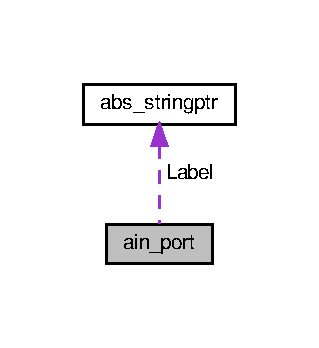
\includegraphics[width=153pt]{d0/d82/structain__port__coll__graph}
\end{center}
\end{figure}
\subsection*{Public Attributes}
\begin{DoxyCompactItemize}
\item 
\hyperlink{ab__common_8h_ae9b1af5c037e57a98884758875d3a7c4}{s32} \hyperlink{structain__port_aa56db8ea0d8c5fea6d6d99c1ed28feee}{Index}
\item 
\hyperlink{structabs__stringptr}{abs\+\_\+stringptr} \hyperlink{structain__port_ac2269d031ae51cd227f87391fba81b1a}{Label}
\end{DoxyCompactItemize}


\subsection{Member Data Documentation}
\mbox{\Hypertarget{structain__port_aa56db8ea0d8c5fea6d6d99c1ed28feee}\label{structain__port_aa56db8ea0d8c5fea6d6d99c1ed28feee}} 
\index{ain\+\_\+port@{ain\+\_\+port}!Index@{Index}}
\index{Index@{Index}!ain\+\_\+port@{ain\+\_\+port}}
\subsubsection{\texorpdfstring{Index}{Index}}
{\footnotesize\ttfamily \hyperlink{ab__common_8h_ae9b1af5c037e57a98884758875d3a7c4}{s32} ain\+\_\+port\+::\+Index}

\mbox{\Hypertarget{structain__port_ac2269d031ae51cd227f87391fba81b1a}\label{structain__port_ac2269d031ae51cd227f87391fba81b1a}} 
\index{ain\+\_\+port@{ain\+\_\+port}!Label@{Label}}
\index{Label@{Label}!ain\+\_\+port@{ain\+\_\+port}}
\subsubsection{\texorpdfstring{Label}{Label}}
{\footnotesize\ttfamily \hyperlink{structabs__stringptr}{abs\+\_\+stringptr} ain\+\_\+port\+::\+Label}



The documentation for this struct was generated from the following file\+:\begin{DoxyCompactItemize}
\item 
\hyperlink{ain__machine_8h}{ain\+\_\+machine.\+h}\end{DoxyCompactItemize}

\hypertarget{structain__state}{}\section{ain\+\_\+state Struct Reference}
\label{structain__state}\index{ain\+\_\+state@{ain\+\_\+state}}


{\ttfamily \#include $<$ain\+\_\+machine.\+h$>$}



Collaboration diagram for ain\+\_\+state\+:\nopagebreak
\begin{figure}[H]
\begin{center}
\leavevmode
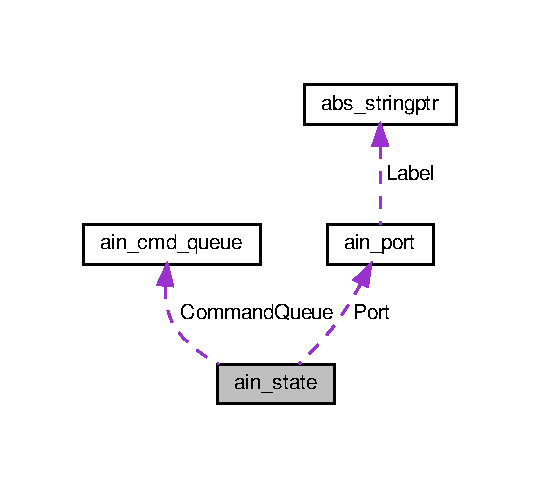
\includegraphics[width=259pt]{dc/d36/structain__state__coll__graph}
\end{center}
\end{figure}
\subsection*{Public Attributes}
\begin{DoxyCompactItemize}
\item 
ain\+\_\+sm $\ast$ \hyperlink{structain__state_a30ffb18e1b012e8b6550901670be0948}{Current\+State}
\item 
\hyperlink{structain__cmd__queue}{ain\+\_\+cmd\+\_\+queue} \hyperlink{structain__state_a60309c1608932df2e5bb8fa9648db68b}{Command\+Queue}
\item 
\hyperlink{ab__common_8h_a70e369648385b50f2d0588e8e8745275}{b8} \hyperlink{structain__state_a8a2bd2b5d34f6e2d3b7a6270a1b88f26}{is\+New\+State}
\item 
\hyperlink{ab__common_8h_ae9b1af5c037e57a98884758875d3a7c4}{s32} \hyperlink{structain__state_ae58221dfcfb85b30d0a2f348e485d377}{File\+Id}
\item 
\hyperlink{ab__common_8h_ae9b1af5c037e57a98884758875d3a7c4}{s32} \hyperlink{structain__state_a367c606e41f41737fc215f46fbed5271}{Read\+Value}
\item 
\hyperlink{ab__time_8h_adc59735fd0d20e93fe3016c8b6a4f782}{abt\+\_\+time} \hyperlink{structain__state_a871210b0691c94540801b72c3a169f0d}{Last\+Read\+Time}
\item 
\hyperlink{structain__port}{ain\+\_\+port} \hyperlink{structain__state_a916756ec631a54c386895526b3e4a1cb}{Port}
\end{DoxyCompactItemize}


\subsection{Member Data Documentation}
\mbox{\Hypertarget{structain__state_a60309c1608932df2e5bb8fa9648db68b}\label{structain__state_a60309c1608932df2e5bb8fa9648db68b}} 
\index{ain\+\_\+state@{ain\+\_\+state}!Command\+Queue@{Command\+Queue}}
\index{Command\+Queue@{Command\+Queue}!ain\+\_\+state@{ain\+\_\+state}}
\subsubsection{\texorpdfstring{Command\+Queue}{CommandQueue}}
{\footnotesize\ttfamily \hyperlink{structain__cmd__queue}{ain\+\_\+cmd\+\_\+queue} ain\+\_\+state\+::\+Command\+Queue}

\mbox{\Hypertarget{structain__state_a30ffb18e1b012e8b6550901670be0948}\label{structain__state_a30ffb18e1b012e8b6550901670be0948}} 
\index{ain\+\_\+state@{ain\+\_\+state}!Current\+State@{Current\+State}}
\index{Current\+State@{Current\+State}!ain\+\_\+state@{ain\+\_\+state}}
\subsubsection{\texorpdfstring{Current\+State}{CurrentState}}
{\footnotesize\ttfamily ain\+\_\+sm$\ast$ ain\+\_\+state\+::\+Current\+State}

\mbox{\Hypertarget{structain__state_ae58221dfcfb85b30d0a2f348e485d377}\label{structain__state_ae58221dfcfb85b30d0a2f348e485d377}} 
\index{ain\+\_\+state@{ain\+\_\+state}!File\+Id@{File\+Id}}
\index{File\+Id@{File\+Id}!ain\+\_\+state@{ain\+\_\+state}}
\subsubsection{\texorpdfstring{File\+Id}{FileId}}
{\footnotesize\ttfamily \hyperlink{ab__common_8h_ae9b1af5c037e57a98884758875d3a7c4}{s32} ain\+\_\+state\+::\+File\+Id}

\mbox{\Hypertarget{structain__state_a8a2bd2b5d34f6e2d3b7a6270a1b88f26}\label{structain__state_a8a2bd2b5d34f6e2d3b7a6270a1b88f26}} 
\index{ain\+\_\+state@{ain\+\_\+state}!is\+New\+State@{is\+New\+State}}
\index{is\+New\+State@{is\+New\+State}!ain\+\_\+state@{ain\+\_\+state}}
\subsubsection{\texorpdfstring{is\+New\+State}{isNewState}}
{\footnotesize\ttfamily \hyperlink{ab__common_8h_a70e369648385b50f2d0588e8e8745275}{b8} ain\+\_\+state\+::is\+New\+State}

\mbox{\Hypertarget{structain__state_a871210b0691c94540801b72c3a169f0d}\label{structain__state_a871210b0691c94540801b72c3a169f0d}} 
\index{ain\+\_\+state@{ain\+\_\+state}!Last\+Read\+Time@{Last\+Read\+Time}}
\index{Last\+Read\+Time@{Last\+Read\+Time}!ain\+\_\+state@{ain\+\_\+state}}
\subsubsection{\texorpdfstring{Last\+Read\+Time}{LastReadTime}}
{\footnotesize\ttfamily \hyperlink{ab__time_8h_adc59735fd0d20e93fe3016c8b6a4f782}{abt\+\_\+time} ain\+\_\+state\+::\+Last\+Read\+Time}

\mbox{\Hypertarget{structain__state_a916756ec631a54c386895526b3e4a1cb}\label{structain__state_a916756ec631a54c386895526b3e4a1cb}} 
\index{ain\+\_\+state@{ain\+\_\+state}!Port@{Port}}
\index{Port@{Port}!ain\+\_\+state@{ain\+\_\+state}}
\subsubsection{\texorpdfstring{Port}{Port}}
{\footnotesize\ttfamily \hyperlink{structain__port}{ain\+\_\+port} ain\+\_\+state\+::\+Port}

\mbox{\Hypertarget{structain__state_a367c606e41f41737fc215f46fbed5271}\label{structain__state_a367c606e41f41737fc215f46fbed5271}} 
\index{ain\+\_\+state@{ain\+\_\+state}!Read\+Value@{Read\+Value}}
\index{Read\+Value@{Read\+Value}!ain\+\_\+state@{ain\+\_\+state}}
\subsubsection{\texorpdfstring{Read\+Value}{ReadValue}}
{\footnotesize\ttfamily \hyperlink{ab__common_8h_ae9b1af5c037e57a98884758875d3a7c4}{s32} ain\+\_\+state\+::\+Read\+Value}



The documentation for this struct was generated from the following file\+:\begin{DoxyCompactItemize}
\item 
\hyperlink{ain__machine_8h}{ain\+\_\+machine.\+h}\end{DoxyCompactItemize}

\hypertarget{structdata}{}\section{data Struct Reference}
\label{structdata}\index{data@{data}}


Collaboration diagram for data\+:
\nopagebreak
\begin{figure}[H]
\begin{center}
\leavevmode
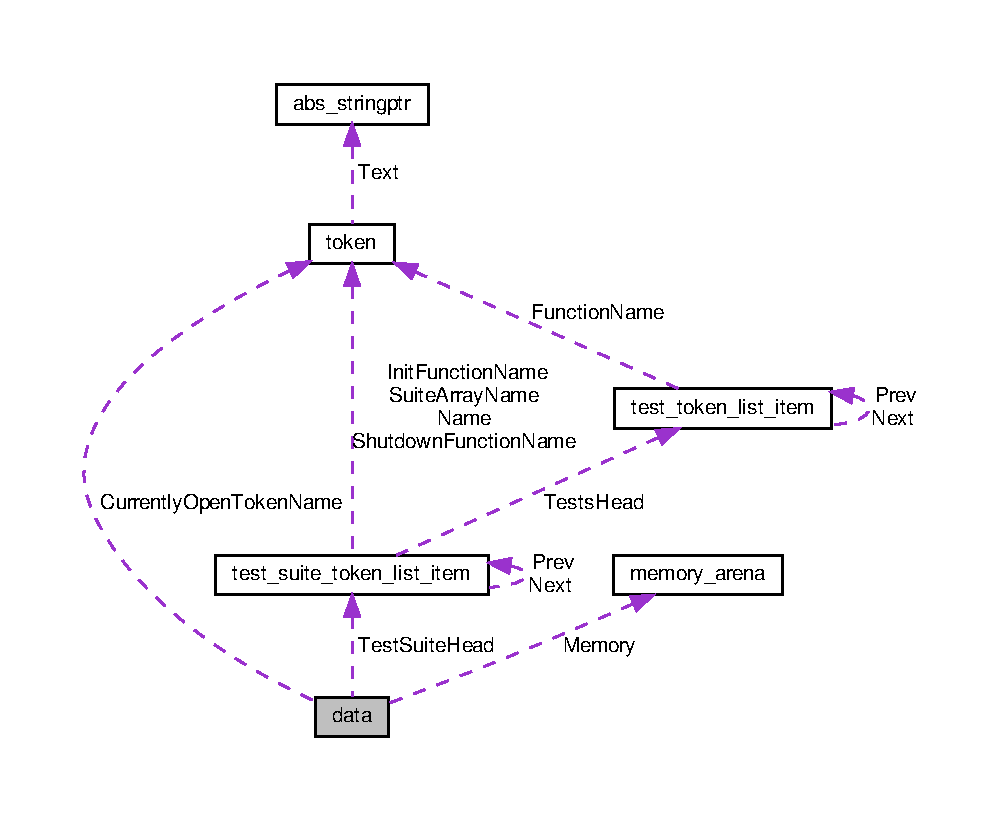
\includegraphics[width=350pt]{d7/dcf/structdata__coll__graph}
\end{center}
\end{figure}
\subsection*{Public Attributes}
\begin{DoxyCompactItemize}
\item 
memory\+\_\+arena \hyperlink{structdata_ad3188e5c8551b604c9d2c3ddbf29a9b8}{Memory}
\item 
\hyperlink{structtoken}{token} \hyperlink{structdata_acd39ca2feac118a8faa8d82520494213}{Currently\+Open\+Token\+Name}
\item 
\hyperlink{structtest__suite__token__list__item}{test\+\_\+suite\+\_\+token\+\_\+list\+\_\+item} \hyperlink{structdata_a5bb01b3754cb4b3baf9b7f499022cd1e}{Test\+Suite\+Head}
\end{DoxyCompactItemize}


\subsection{Member Data Documentation}
\mbox{\Hypertarget{structdata_acd39ca2feac118a8faa8d82520494213}\label{structdata_acd39ca2feac118a8faa8d82520494213}} 
\index{data@{data}!Currently\+Open\+Token\+Name@{Currently\+Open\+Token\+Name}}
\index{Currently\+Open\+Token\+Name@{Currently\+Open\+Token\+Name}!data@{data}}
\subsubsection{\texorpdfstring{Currently\+Open\+Token\+Name}{CurrentlyOpenTokenName}}
{\footnotesize\ttfamily \hyperlink{structtoken}{token} data\+::\+Currently\+Open\+Token\+Name}

\mbox{\Hypertarget{structdata_ad3188e5c8551b604c9d2c3ddbf29a9b8}\label{structdata_ad3188e5c8551b604c9d2c3ddbf29a9b8}} 
\index{data@{data}!Memory@{Memory}}
\index{Memory@{Memory}!data@{data}}
\subsubsection{\texorpdfstring{Memory}{Memory}}
{\footnotesize\ttfamily memory\+\_\+arena data\+::\+Memory}

\mbox{\Hypertarget{structdata_a5bb01b3754cb4b3baf9b7f499022cd1e}\label{structdata_a5bb01b3754cb4b3baf9b7f499022cd1e}} 
\index{data@{data}!Test\+Suite\+Head@{Test\+Suite\+Head}}
\index{Test\+Suite\+Head@{Test\+Suite\+Head}!data@{data}}
\subsubsection{\texorpdfstring{Test\+Suite\+Head}{TestSuiteHead}}
{\footnotesize\ttfamily \hyperlink{structtest__suite__token__list__item}{test\+\_\+suite\+\_\+token\+\_\+list\+\_\+item} data\+::\+Test\+Suite\+Head}



The documentation for this struct was generated from the following file\+:\begin{DoxyCompactItemize}
\item 
\hyperlink{test__preprocessor_8cpp}{test\+\_\+preprocessor.\+cpp}\end{DoxyCompactItemize}

\hypertarget{structdio__cmd__queue}{}\section{dio\+\_\+cmd\+\_\+queue Struct Reference}
\label{structdio__cmd__queue}\index{dio\+\_\+cmd\+\_\+queue@{dio\+\_\+cmd\+\_\+queue}}


{\ttfamily \#include $<$Generated\+\_\+001.\+h$>$}

\subsection*{Public Attributes}
\begin{DoxyCompactItemize}
\item 
\hyperlink{dio__machine_8h_ac4b00fe9f70ff379f2ca79f1ac7828c4}{dio\+\_\+cmd} \hyperlink{structdio__cmd__queue_a29e9979e5bce86dab10b248bea3ca3c6}{Items} \mbox{[}10\mbox{]}
\item 
\hyperlink{ab__common_8h_ae9b1af5c037e57a98884758875d3a7c4}{s32} \hyperlink{structdio__cmd__queue_a15b4f61ae434e3d621f1d6ac227cd4d0}{Front}
\item 
\hyperlink{ab__common_8h_ae9b1af5c037e57a98884758875d3a7c4}{s32} \hyperlink{structdio__cmd__queue_a5669f4099d38a9344b6e6ab1982b1822}{Rear}
\end{DoxyCompactItemize}


\subsection{Member Data Documentation}
\mbox{\Hypertarget{structdio__cmd__queue_a15b4f61ae434e3d621f1d6ac227cd4d0}\label{structdio__cmd__queue_a15b4f61ae434e3d621f1d6ac227cd4d0}} 
\index{dio\+\_\+cmd\+\_\+queue@{dio\+\_\+cmd\+\_\+queue}!Front@{Front}}
\index{Front@{Front}!dio\+\_\+cmd\+\_\+queue@{dio\+\_\+cmd\+\_\+queue}}
\subsubsection{\texorpdfstring{Front}{Front}}
{\footnotesize\ttfamily \hyperlink{ab__common_8h_ae9b1af5c037e57a98884758875d3a7c4}{s32} dio\+\_\+cmd\+\_\+queue\+::\+Front}

\mbox{\Hypertarget{structdio__cmd__queue_a29e9979e5bce86dab10b248bea3ca3c6}\label{structdio__cmd__queue_a29e9979e5bce86dab10b248bea3ca3c6}} 
\index{dio\+\_\+cmd\+\_\+queue@{dio\+\_\+cmd\+\_\+queue}!Items@{Items}}
\index{Items@{Items}!dio\+\_\+cmd\+\_\+queue@{dio\+\_\+cmd\+\_\+queue}}
\subsubsection{\texorpdfstring{Items}{Items}}
{\footnotesize\ttfamily \hyperlink{dio__machine_8h_ac4b00fe9f70ff379f2ca79f1ac7828c4}{dio\+\_\+cmd} dio\+\_\+cmd\+\_\+queue\+::\+Items\mbox{[}10\mbox{]}}

\mbox{\Hypertarget{structdio__cmd__queue_a5669f4099d38a9344b6e6ab1982b1822}\label{structdio__cmd__queue_a5669f4099d38a9344b6e6ab1982b1822}} 
\index{dio\+\_\+cmd\+\_\+queue@{dio\+\_\+cmd\+\_\+queue}!Rear@{Rear}}
\index{Rear@{Rear}!dio\+\_\+cmd\+\_\+queue@{dio\+\_\+cmd\+\_\+queue}}
\subsubsection{\texorpdfstring{Rear}{Rear}}
{\footnotesize\ttfamily \hyperlink{ab__common_8h_ae9b1af5c037e57a98884758875d3a7c4}{s32} dio\+\_\+cmd\+\_\+queue\+::\+Rear}



The documentation for this struct was generated from the following file\+:\begin{DoxyCompactItemize}
\item 
\hyperlink{Generated__001_8h}{Generated\+\_\+001.\+h}\end{DoxyCompactItemize}

\hypertarget{structdio__port}{}\section{dio\+\_\+port Struct Reference}
\label{structdio__port}\index{dio\+\_\+port@{dio\+\_\+port}}


{\ttfamily \#include $<$dio\+\_\+machine.\+h$>$}



Collaboration diagram for dio\+\_\+port\+:\nopagebreak
\begin{figure}[H]
\begin{center}
\leavevmode
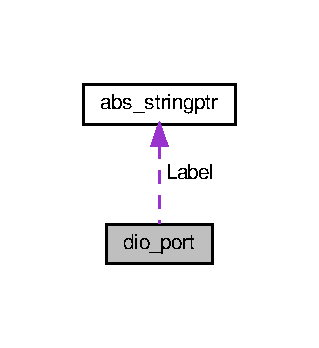
\includegraphics[width=153pt]{d1/d3a/structdio__port__coll__graph}
\end{center}
\end{figure}
\subsection*{Public Attributes}
\begin{DoxyCompactItemize}
\item 
\hyperlink{ab__common_8h_ae9b1af5c037e57a98884758875d3a7c4}{s32} \hyperlink{structdio__port_a4cad63c96a1b03d4e85d107781a119c7}{Pin}
\item 
\hyperlink{structabs__stringptr}{abs\+\_\+stringptr} \hyperlink{structdio__port_a9135b29613e9dee6b732d3662764f4a2}{Label}
\item 
\hyperlink{adsio_8h_a99f26e6ee9fcd62f75203b5402df8098}{direction} \hyperlink{structdio__port_a2a5027ad90ea005ad1cd90ec35d42271}{Direction}
\end{DoxyCompactItemize}


\subsection{Member Data Documentation}
\mbox{\Hypertarget{structdio__port_a2a5027ad90ea005ad1cd90ec35d42271}\label{structdio__port_a2a5027ad90ea005ad1cd90ec35d42271}} 
\index{dio\+\_\+port@{dio\+\_\+port}!Direction@{Direction}}
\index{Direction@{Direction}!dio\+\_\+port@{dio\+\_\+port}}
\subsubsection{\texorpdfstring{Direction}{Direction}}
{\footnotesize\ttfamily \hyperlink{adsio_8h_a99f26e6ee9fcd62f75203b5402df8098}{direction} dio\+\_\+port\+::\+Direction}

\mbox{\Hypertarget{structdio__port_a9135b29613e9dee6b732d3662764f4a2}\label{structdio__port_a9135b29613e9dee6b732d3662764f4a2}} 
\index{dio\+\_\+port@{dio\+\_\+port}!Label@{Label}}
\index{Label@{Label}!dio\+\_\+port@{dio\+\_\+port}}
\subsubsection{\texorpdfstring{Label}{Label}}
{\footnotesize\ttfamily \hyperlink{structabs__stringptr}{abs\+\_\+stringptr} dio\+\_\+port\+::\+Label}

\mbox{\Hypertarget{structdio__port_a4cad63c96a1b03d4e85d107781a119c7}\label{structdio__port_a4cad63c96a1b03d4e85d107781a119c7}} 
\index{dio\+\_\+port@{dio\+\_\+port}!Pin@{Pin}}
\index{Pin@{Pin}!dio\+\_\+port@{dio\+\_\+port}}
\subsubsection{\texorpdfstring{Pin}{Pin}}
{\footnotesize\ttfamily \hyperlink{ab__common_8h_ae9b1af5c037e57a98884758875d3a7c4}{s32} dio\+\_\+port\+::\+Pin}



The documentation for this struct was generated from the following file\+:\begin{DoxyCompactItemize}
\item 
\hyperlink{dio__machine_8h}{dio\+\_\+machine.\+h}\end{DoxyCompactItemize}

\hypertarget{structdio__state}{}\section{dio\+\_\+state Struct Reference}
\label{structdio__state}\index{dio\+\_\+state@{dio\+\_\+state}}


{\ttfamily \#include $<$dio\+\_\+machine.\+h$>$}



Collaboration diagram for dio\+\_\+state\+:\nopagebreak
\begin{figure}[H]
\begin{center}
\leavevmode
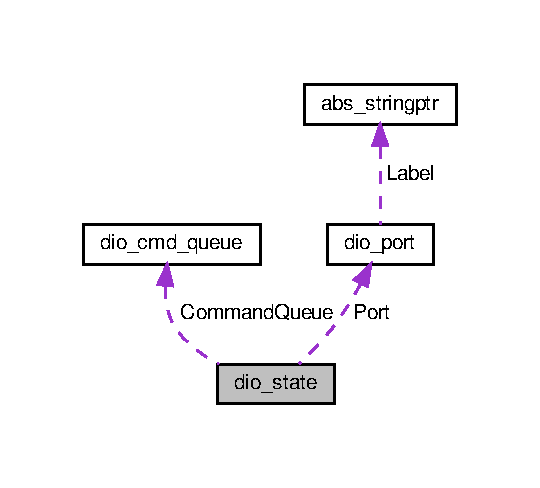
\includegraphics[width=259pt]{d4/ded/structdio__state__coll__graph}
\end{center}
\end{figure}
\subsection*{Public Attributes}
\begin{DoxyCompactItemize}
\item 
dio\+\_\+sm $\ast$ \hyperlink{structdio__state_a3e4d69566fe3663715242717832047ad}{Current\+State}
\item 
\hyperlink{structdio__cmd__queue}{dio\+\_\+cmd\+\_\+queue} \hyperlink{structdio__state_a01f7ae8045204bd943279d573c380620}{Command\+Queue}
\item 
\hyperlink{ab__common_8h_a70e369648385b50f2d0588e8e8745275}{b8} \hyperlink{structdio__state_a6932dd0222d575db057e77a1df47613b}{is\+New\+State}
\item 
\hyperlink{adsio_8h_a20884447391b4598296c73c6fa3d9470}{Tri\+State} \hyperlink{structdio__state_aaa849b5fd1e89616a2a0ad749231f3eb}{Read\+Value}
\item 
\hyperlink{adsio_8h_a20884447391b4598296c73c6fa3d9470}{Tri\+State} \hyperlink{structdio__state_a814fbbc0fd796a5aa5069c5e2da472ad}{to\+Write\+Value}
\item 
\hyperlink{ab__common_8h_ae9b1af5c037e57a98884758875d3a7c4}{s32} \hyperlink{structdio__state_afe0f18233c967a8f31eefe0a1aa7c542}{File\+Id}
\item 
\hyperlink{ab__time_8h_adc59735fd0d20e93fe3016c8b6a4f782}{abt\+\_\+time} \hyperlink{structdio__state_a0646772523d6d065607ca118ffe732cc}{Last\+Read\+Time}
\item 
\hyperlink{ab__common_8h_ae9b1af5c037e57a98884758875d3a7c4}{s32} \hyperlink{structdio__state_aea2fdc28a78a6281357be92204fa5f47}{File\+Error}
\item 
\hyperlink{structdio__port}{dio\+\_\+port} \hyperlink{structdio__state_a9e0dd820a840b52e4696c5f782b0be25}{Port}
\end{DoxyCompactItemize}


\subsection{Member Data Documentation}
\mbox{\Hypertarget{structdio__state_a01f7ae8045204bd943279d573c380620}\label{structdio__state_a01f7ae8045204bd943279d573c380620}} 
\index{dio\+\_\+state@{dio\+\_\+state}!Command\+Queue@{Command\+Queue}}
\index{Command\+Queue@{Command\+Queue}!dio\+\_\+state@{dio\+\_\+state}}
\subsubsection{\texorpdfstring{Command\+Queue}{CommandQueue}}
{\footnotesize\ttfamily \hyperlink{structdio__cmd__queue}{dio\+\_\+cmd\+\_\+queue} dio\+\_\+state\+::\+Command\+Queue}

\mbox{\Hypertarget{structdio__state_a3e4d69566fe3663715242717832047ad}\label{structdio__state_a3e4d69566fe3663715242717832047ad}} 
\index{dio\+\_\+state@{dio\+\_\+state}!Current\+State@{Current\+State}}
\index{Current\+State@{Current\+State}!dio\+\_\+state@{dio\+\_\+state}}
\subsubsection{\texorpdfstring{Current\+State}{CurrentState}}
{\footnotesize\ttfamily dio\+\_\+sm$\ast$ dio\+\_\+state\+::\+Current\+State}

\mbox{\Hypertarget{structdio__state_aea2fdc28a78a6281357be92204fa5f47}\label{structdio__state_aea2fdc28a78a6281357be92204fa5f47}} 
\index{dio\+\_\+state@{dio\+\_\+state}!File\+Error@{File\+Error}}
\index{File\+Error@{File\+Error}!dio\+\_\+state@{dio\+\_\+state}}
\subsubsection{\texorpdfstring{File\+Error}{FileError}}
{\footnotesize\ttfamily \hyperlink{ab__common_8h_ae9b1af5c037e57a98884758875d3a7c4}{s32} dio\+\_\+state\+::\+File\+Error}

\mbox{\Hypertarget{structdio__state_afe0f18233c967a8f31eefe0a1aa7c542}\label{structdio__state_afe0f18233c967a8f31eefe0a1aa7c542}} 
\index{dio\+\_\+state@{dio\+\_\+state}!File\+Id@{File\+Id}}
\index{File\+Id@{File\+Id}!dio\+\_\+state@{dio\+\_\+state}}
\subsubsection{\texorpdfstring{File\+Id}{FileId}}
{\footnotesize\ttfamily \hyperlink{ab__common_8h_ae9b1af5c037e57a98884758875d3a7c4}{s32} dio\+\_\+state\+::\+File\+Id}

\mbox{\Hypertarget{structdio__state_a6932dd0222d575db057e77a1df47613b}\label{structdio__state_a6932dd0222d575db057e77a1df47613b}} 
\index{dio\+\_\+state@{dio\+\_\+state}!is\+New\+State@{is\+New\+State}}
\index{is\+New\+State@{is\+New\+State}!dio\+\_\+state@{dio\+\_\+state}}
\subsubsection{\texorpdfstring{is\+New\+State}{isNewState}}
{\footnotesize\ttfamily \hyperlink{ab__common_8h_a70e369648385b50f2d0588e8e8745275}{b8} dio\+\_\+state\+::is\+New\+State}

\mbox{\Hypertarget{structdio__state_a0646772523d6d065607ca118ffe732cc}\label{structdio__state_a0646772523d6d065607ca118ffe732cc}} 
\index{dio\+\_\+state@{dio\+\_\+state}!Last\+Read\+Time@{Last\+Read\+Time}}
\index{Last\+Read\+Time@{Last\+Read\+Time}!dio\+\_\+state@{dio\+\_\+state}}
\subsubsection{\texorpdfstring{Last\+Read\+Time}{LastReadTime}}
{\footnotesize\ttfamily \hyperlink{ab__time_8h_adc59735fd0d20e93fe3016c8b6a4f782}{abt\+\_\+time} dio\+\_\+state\+::\+Last\+Read\+Time}

\mbox{\Hypertarget{structdio__state_a9e0dd820a840b52e4696c5f782b0be25}\label{structdio__state_a9e0dd820a840b52e4696c5f782b0be25}} 
\index{dio\+\_\+state@{dio\+\_\+state}!Port@{Port}}
\index{Port@{Port}!dio\+\_\+state@{dio\+\_\+state}}
\subsubsection{\texorpdfstring{Port}{Port}}
{\footnotesize\ttfamily \hyperlink{structdio__port}{dio\+\_\+port} dio\+\_\+state\+::\+Port}

\mbox{\Hypertarget{structdio__state_aaa849b5fd1e89616a2a0ad749231f3eb}\label{structdio__state_aaa849b5fd1e89616a2a0ad749231f3eb}} 
\index{dio\+\_\+state@{dio\+\_\+state}!Read\+Value@{Read\+Value}}
\index{Read\+Value@{Read\+Value}!dio\+\_\+state@{dio\+\_\+state}}
\subsubsection{\texorpdfstring{Read\+Value}{ReadValue}}
{\footnotesize\ttfamily \hyperlink{adsio_8h_a20884447391b4598296c73c6fa3d9470}{Tri\+State} dio\+\_\+state\+::\+Read\+Value}

\mbox{\Hypertarget{structdio__state_a814fbbc0fd796a5aa5069c5e2da472ad}\label{structdio__state_a814fbbc0fd796a5aa5069c5e2da472ad}} 
\index{dio\+\_\+state@{dio\+\_\+state}!to\+Write\+Value@{to\+Write\+Value}}
\index{to\+Write\+Value@{to\+Write\+Value}!dio\+\_\+state@{dio\+\_\+state}}
\subsubsection{\texorpdfstring{to\+Write\+Value}{toWriteValue}}
{\footnotesize\ttfamily \hyperlink{adsio_8h_a20884447391b4598296c73c6fa3d9470}{Tri\+State} dio\+\_\+state\+::to\+Write\+Value}



The documentation for this struct was generated from the following file\+:\begin{DoxyCompactItemize}
\item 
\hyperlink{dio__machine_8h}{dio\+\_\+machine.\+h}\end{DoxyCompactItemize}

\hypertarget{structfile__data}{}\doxysection{file\+\_\+data Struct Reference}
\label{structfile__data}\index{file\_data@{file\_data}}


{\ttfamily \#include $<$ab\+\_\+file.\+h$>$}

\doxysubsection*{Public Attributes}
\begin{DoxyCompactItemize}
\item 
size\+\_\+t \mbox{\hyperlink{structfile__data_a72812241b55929a508538f596b52b7d7}{Size}}
\item 
u32 \mbox{\hyperlink{structfile__data_a8b5a3e4d5881e29760e77ac06d7f37c1}{File\+Index}}
\item 
char \mbox{\hyperlink{structfile__data_a3a1dc6a36635557387bc2f0c2e99b2b2}{File\+Name}} \mbox{[}\mbox{\hyperlink{ab__file_8h_ab99ded389af74001a6298fc9e44e74e5}{M\+A\+X\+\_\+\+P\+A\+TH}}\mbox{]}
\item 
char $\ast$ \mbox{\hyperlink{structfile__data_ab28b5cd0a1d3c6a5ecaddd7365012758}{File\+Data}}
\item 
\mbox{\hyperlink{ab__file_8h_a1b665fc63cb310d53283fbcd1b19746e}{en\+File\+Type}} \mbox{\hyperlink{structfile__data_a08ce87775b0af51c6462c969706cf58e}{Type}}
\end{DoxyCompactItemize}


\doxysubsection{Member Data Documentation}
\mbox{\Hypertarget{structfile__data_ab28b5cd0a1d3c6a5ecaddd7365012758}\label{structfile__data_ab28b5cd0a1d3c6a5ecaddd7365012758}} 
\index{file\_data@{file\_data}!FileData@{FileData}}
\index{FileData@{FileData}!file\_data@{file\_data}}
\doxysubsubsection{\texorpdfstring{FileData}{FileData}}
{\footnotesize\ttfamily char$\ast$ file\+\_\+data\+::\+File\+Data}

\mbox{\Hypertarget{structfile__data_a8b5a3e4d5881e29760e77ac06d7f37c1}\label{structfile__data_a8b5a3e4d5881e29760e77ac06d7f37c1}} 
\index{file\_data@{file\_data}!FileIndex@{FileIndex}}
\index{FileIndex@{FileIndex}!file\_data@{file\_data}}
\doxysubsubsection{\texorpdfstring{FileIndex}{FileIndex}}
{\footnotesize\ttfamily u32 file\+\_\+data\+::\+File\+Index}

\mbox{\Hypertarget{structfile__data_a3a1dc6a36635557387bc2f0c2e99b2b2}\label{structfile__data_a3a1dc6a36635557387bc2f0c2e99b2b2}} 
\index{file\_data@{file\_data}!FileName@{FileName}}
\index{FileName@{FileName}!file\_data@{file\_data}}
\doxysubsubsection{\texorpdfstring{FileName}{FileName}}
{\footnotesize\ttfamily char file\+\_\+data\+::\+File\+Name\mbox{[}\mbox{\hyperlink{ab__file_8h_ab99ded389af74001a6298fc9e44e74e5}{M\+A\+X\+\_\+\+P\+A\+TH}}\mbox{]}}

\mbox{\Hypertarget{structfile__data_a72812241b55929a508538f596b52b7d7}\label{structfile__data_a72812241b55929a508538f596b52b7d7}} 
\index{file\_data@{file\_data}!Size@{Size}}
\index{Size@{Size}!file\_data@{file\_data}}
\doxysubsubsection{\texorpdfstring{Size}{Size}}
{\footnotesize\ttfamily size\+\_\+t file\+\_\+data\+::\+Size}

\mbox{\Hypertarget{structfile__data_a08ce87775b0af51c6462c969706cf58e}\label{structfile__data_a08ce87775b0af51c6462c969706cf58e}} 
\index{file\_data@{file\_data}!Type@{Type}}
\index{Type@{Type}!file\_data@{file\_data}}
\doxysubsubsection{\texorpdfstring{Type}{Type}}
{\footnotesize\ttfamily \mbox{\hyperlink{ab__file_8h_a1b665fc63cb310d53283fbcd1b19746e}{en\+File\+Type}} file\+\_\+data\+::\+Type}



The documentation for this struct was generated from the following file\+:\begin{DoxyCompactItemize}
\item 
\mbox{\hyperlink{ab__file_8h}{ab\+\_\+file.\+h}}\end{DoxyCompactItemize}

\hypertarget{structfile__list}{}\section{file\+\_\+list Struct Reference}
\label{structfile__list}\index{file\+\_\+list@{file\+\_\+list}}


{\ttfamily \#include $<$ab\+\_\+file\+\_\+linux.\+h$>$}



Collaboration diagram for file\+\_\+list\+:\nopagebreak
\begin{figure}[H]
\begin{center}
\leavevmode
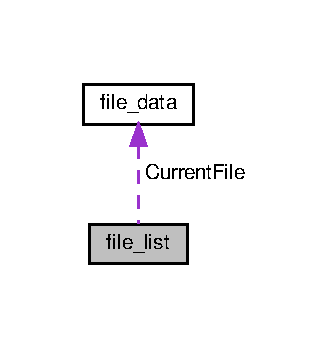
\includegraphics[width=159pt]{d8/df1/structfile__list__coll__graph}
\end{center}
\end{figure}
\subsection*{Public Attributes}
\begin{DoxyCompactItemize}
\item 
glob\+\_\+t \hyperlink{structfile__list_a8b9c52b0dbeb615a3d2ec8c4e75fce49}{Glob\+Data}
\item 
size\+\_\+t \hyperlink{structfile__list_a1f88f1b450c176c81c7ffdd7d5334429}{File\+Count}
\item 
\hyperlink{ab__common_8h_afaa62991928fb9fb18ff0db62a040aba}{u32} \hyperlink{structfile__list_a18a2bcd2708d290b02cb3a80a3f68d48}{File\+Index}
\item 
\hyperlink{structfile__data}{file\+\_\+data} $\ast$ \hyperlink{structfile__list_a8103a737b7c8edc9da8dfa5c75abe242}{Current\+File}
\item 
char \hyperlink{structfile__list_a50f2703df63faf3266542b422b417cd9}{Path} \mbox{[}\hyperlink{ab__file_8h_ab99ded389af74001a6298fc9e44e74e5}{M\+A\+X\+\_\+\+P\+A\+TH}\mbox{]}
\item 
H\+A\+N\+D\+LE \hyperlink{structfile__list_a890b377545055c3acb0d705ea20a13c4}{File\+Search\+Handle}
\item 
\hyperlink{ab__common_8h_a70e369648385b50f2d0588e8e8745275}{b8} \hyperlink{structfile__list_ab563e99003e66a0dbee5f5e4a4129b84}{is\+Dir\+Valid}
\end{DoxyCompactItemize}


\subsection{Member Data Documentation}
\mbox{\Hypertarget{structfile__list_a8103a737b7c8edc9da8dfa5c75abe242}\label{structfile__list_a8103a737b7c8edc9da8dfa5c75abe242}} 
\index{file\+\_\+list@{file\+\_\+list}!Current\+File@{Current\+File}}
\index{Current\+File@{Current\+File}!file\+\_\+list@{file\+\_\+list}}
\subsubsection{\texorpdfstring{Current\+File}{CurrentFile}}
{\footnotesize\ttfamily \hyperlink{structfile__data}{file\+\_\+data} $\ast$ file\+\_\+list\+::\+Current\+File}

\mbox{\Hypertarget{structfile__list_a1f88f1b450c176c81c7ffdd7d5334429}\label{structfile__list_a1f88f1b450c176c81c7ffdd7d5334429}} 
\index{file\+\_\+list@{file\+\_\+list}!File\+Count@{File\+Count}}
\index{File\+Count@{File\+Count}!file\+\_\+list@{file\+\_\+list}}
\subsubsection{\texorpdfstring{File\+Count}{FileCount}}
{\footnotesize\ttfamily size\+\_\+t file\+\_\+list\+::\+File\+Count}

\mbox{\Hypertarget{structfile__list_a18a2bcd2708d290b02cb3a80a3f68d48}\label{structfile__list_a18a2bcd2708d290b02cb3a80a3f68d48}} 
\index{file\+\_\+list@{file\+\_\+list}!File\+Index@{File\+Index}}
\index{File\+Index@{File\+Index}!file\+\_\+list@{file\+\_\+list}}
\subsubsection{\texorpdfstring{File\+Index}{FileIndex}}
{\footnotesize\ttfamily \hyperlink{ab__common_8h_afaa62991928fb9fb18ff0db62a040aba}{u32} file\+\_\+list\+::\+File\+Index}

\mbox{\Hypertarget{structfile__list_a890b377545055c3acb0d705ea20a13c4}\label{structfile__list_a890b377545055c3acb0d705ea20a13c4}} 
\index{file\+\_\+list@{file\+\_\+list}!File\+Search\+Handle@{File\+Search\+Handle}}
\index{File\+Search\+Handle@{File\+Search\+Handle}!file\+\_\+list@{file\+\_\+list}}
\subsubsection{\texorpdfstring{File\+Search\+Handle}{FileSearchHandle}}
{\footnotesize\ttfamily H\+A\+N\+D\+LE file\+\_\+list\+::\+File\+Search\+Handle}

\mbox{\Hypertarget{structfile__list_a8b9c52b0dbeb615a3d2ec8c4e75fce49}\label{structfile__list_a8b9c52b0dbeb615a3d2ec8c4e75fce49}} 
\index{file\+\_\+list@{file\+\_\+list}!Glob\+Data@{Glob\+Data}}
\index{Glob\+Data@{Glob\+Data}!file\+\_\+list@{file\+\_\+list}}
\subsubsection{\texorpdfstring{Glob\+Data}{GlobData}}
{\footnotesize\ttfamily glob\+\_\+t file\+\_\+list\+::\+Glob\+Data}

\mbox{\Hypertarget{structfile__list_ab563e99003e66a0dbee5f5e4a4129b84}\label{structfile__list_ab563e99003e66a0dbee5f5e4a4129b84}} 
\index{file\+\_\+list@{file\+\_\+list}!is\+Dir\+Valid@{is\+Dir\+Valid}}
\index{is\+Dir\+Valid@{is\+Dir\+Valid}!file\+\_\+list@{file\+\_\+list}}
\subsubsection{\texorpdfstring{is\+Dir\+Valid}{isDirValid}}
{\footnotesize\ttfamily \hyperlink{ab__common_8h_a70e369648385b50f2d0588e8e8745275}{b8} file\+\_\+list\+::is\+Dir\+Valid}

\mbox{\Hypertarget{structfile__list_a50f2703df63faf3266542b422b417cd9}\label{structfile__list_a50f2703df63faf3266542b422b417cd9}} 
\index{file\+\_\+list@{file\+\_\+list}!Path@{Path}}
\index{Path@{Path}!file\+\_\+list@{file\+\_\+list}}
\subsubsection{\texorpdfstring{Path}{Path}}
{\footnotesize\ttfamily char file\+\_\+list\+::\+Path}



The documentation for this struct was generated from the following files\+:\begin{DoxyCompactItemize}
\item 
\hyperlink{ab__file__linux_8h}{ab\+\_\+file\+\_\+linux.\+h}\item 
\hyperlink{ab__file__win32_8h}{ab\+\_\+file\+\_\+win32.\+h}\end{DoxyCompactItemize}

\hypertarget{structio__data}{}\section{io\+\_\+data Struct Reference}
\label{structio__data}\index{io\+\_\+data@{io\+\_\+data}}


{\ttfamily \#include $<$adsio.\+h$>$}

\subsection*{Public Attributes}
\begin{DoxyCompactItemize}
\item 
\hyperlink{ab__common_8h_ae9b1af5c037e57a98884758875d3a7c4}{s32} \hyperlink{structio__data_a9171c6d890faeea3eba2aa87600d0975}{Value}
\item 
\hyperlink{ab__time_8h_adc59735fd0d20e93fe3016c8b6a4f782}{abt\+\_\+time} \hyperlink{structio__data_a9f49c3a9e68a9959ed47b179d8a47a84}{Time}
\end{DoxyCompactItemize}


\subsection{Member Data Documentation}
\mbox{\Hypertarget{structio__data_a9f49c3a9e68a9959ed47b179d8a47a84}\label{structio__data_a9f49c3a9e68a9959ed47b179d8a47a84}} 
\index{io\+\_\+data@{io\+\_\+data}!Time@{Time}}
\index{Time@{Time}!io\+\_\+data@{io\+\_\+data}}
\subsubsection{\texorpdfstring{Time}{Time}}
{\footnotesize\ttfamily \hyperlink{ab__time_8h_adc59735fd0d20e93fe3016c8b6a4f782}{abt\+\_\+time} io\+\_\+data\+::\+Time}

\mbox{\Hypertarget{structio__data_a9171c6d890faeea3eba2aa87600d0975}\label{structio__data_a9171c6d890faeea3eba2aa87600d0975}} 
\index{io\+\_\+data@{io\+\_\+data}!Value@{Value}}
\index{Value@{Value}!io\+\_\+data@{io\+\_\+data}}
\subsubsection{\texorpdfstring{Value}{Value}}
{\footnotesize\ttfamily \hyperlink{ab__common_8h_ae9b1af5c037e57a98884758875d3a7c4}{s32} io\+\_\+data\+::\+Value}



The documentation for this struct was generated from the following file\+:\begin{DoxyCompactItemize}
\item 
\hyperlink{adsio_8h}{adsio.\+h}\end{DoxyCompactItemize}

\hypertarget{structjsmn__parser}{}\section{jsmn\+\_\+parser Struct Reference}
\label{structjsmn__parser}\index{jsmn\+\_\+parser@{jsmn\+\_\+parser}}


{\ttfamily \#include $<$jsmn.\+h$>$}

\subsection*{Public Attributes}
\begin{DoxyCompactItemize}
\item 
unsigned int \hyperlink{structjsmn__parser_a3d0d6e48d3d5b24262f9e0c2241dc456}{pos}
\item 
unsigned int \hyperlink{structjsmn__parser_af640efd7d154218124a964b65f114bff}{toknext}
\item 
int \hyperlink{structjsmn__parser_af11fcec48d9f1298909777a12f1d1e39}{toksuper}
\end{DoxyCompactItemize}


\subsection{Detailed Description}
J\+S\+ON parser. Contains an array of token blocks available. Also stores the string being parsed now and current position in that string. 

\subsection{Member Data Documentation}
\mbox{\Hypertarget{structjsmn__parser_a3d0d6e48d3d5b24262f9e0c2241dc456}\label{structjsmn__parser_a3d0d6e48d3d5b24262f9e0c2241dc456}} 
\index{jsmn\+\_\+parser@{jsmn\+\_\+parser}!pos@{pos}}
\index{pos@{pos}!jsmn\+\_\+parser@{jsmn\+\_\+parser}}
\subsubsection{\texorpdfstring{pos}{pos}}
{\footnotesize\ttfamily unsigned int jsmn\+\_\+parser\+::pos}

\mbox{\Hypertarget{structjsmn__parser_af640efd7d154218124a964b65f114bff}\label{structjsmn__parser_af640efd7d154218124a964b65f114bff}} 
\index{jsmn\+\_\+parser@{jsmn\+\_\+parser}!toknext@{toknext}}
\index{toknext@{toknext}!jsmn\+\_\+parser@{jsmn\+\_\+parser}}
\subsubsection{\texorpdfstring{toknext}{toknext}}
{\footnotesize\ttfamily unsigned int jsmn\+\_\+parser\+::toknext}

\mbox{\Hypertarget{structjsmn__parser_af11fcec48d9f1298909777a12f1d1e39}\label{structjsmn__parser_af11fcec48d9f1298909777a12f1d1e39}} 
\index{jsmn\+\_\+parser@{jsmn\+\_\+parser}!toksuper@{toksuper}}
\index{toksuper@{toksuper}!jsmn\+\_\+parser@{jsmn\+\_\+parser}}
\subsubsection{\texorpdfstring{toksuper}{toksuper}}
{\footnotesize\ttfamily int jsmn\+\_\+parser\+::toksuper}



The documentation for this struct was generated from the following file\+:\begin{DoxyCompactItemize}
\item 
\hyperlink{include_2jsmn_8h}{include/jsmn.\+h}\end{DoxyCompactItemize}

\hypertarget{structjsmntok__t}{}\section{jsmntok\+\_\+t Struct Reference}
\label{structjsmntok__t}\index{jsmntok\+\_\+t@{jsmntok\+\_\+t}}


{\ttfamily \#include $<$jsmn.\+h$>$}

\subsection*{Public Attributes}
\begin{DoxyCompactItemize}
\item 
\hyperlink{include_2jsmn_8h_a065320719769f9dc1fbe30094e52802f}{jsmntype\+\_\+t} \hyperlink{structjsmntok__t_ac03dbd6b83cbcd979eb64702d5b9943e}{type}
\item 
int \hyperlink{structjsmntok__t_a0a8f55d0095f268ce8e224fe1234acd0}{start}
\item 
int \hyperlink{structjsmntok__t_ab49e0369f39e9b6174141e7f5bde5996}{end}
\item 
int \hyperlink{structjsmntok__t_a8ac3694b7335456c8e602197778883db}{size}
\end{DoxyCompactItemize}


\subsection{Detailed Description}
J\+S\+ON token description. type type (object, array, string etc.) start start position in J\+S\+ON data string end end position in J\+S\+ON data string 

\subsection{Member Data Documentation}
\mbox{\Hypertarget{structjsmntok__t_ab49e0369f39e9b6174141e7f5bde5996}\label{structjsmntok__t_ab49e0369f39e9b6174141e7f5bde5996}} 
\index{jsmntok\+\_\+t@{jsmntok\+\_\+t}!end@{end}}
\index{end@{end}!jsmntok\+\_\+t@{jsmntok\+\_\+t}}
\subsubsection{\texorpdfstring{end}{end}}
{\footnotesize\ttfamily int jsmntok\+\_\+t\+::end}

\mbox{\Hypertarget{structjsmntok__t_a8ac3694b7335456c8e602197778883db}\label{structjsmntok__t_a8ac3694b7335456c8e602197778883db}} 
\index{jsmntok\+\_\+t@{jsmntok\+\_\+t}!size@{size}}
\index{size@{size}!jsmntok\+\_\+t@{jsmntok\+\_\+t}}
\subsubsection{\texorpdfstring{size}{size}}
{\footnotesize\ttfamily int jsmntok\+\_\+t\+::size}

\mbox{\Hypertarget{structjsmntok__t_a0a8f55d0095f268ce8e224fe1234acd0}\label{structjsmntok__t_a0a8f55d0095f268ce8e224fe1234acd0}} 
\index{jsmntok\+\_\+t@{jsmntok\+\_\+t}!start@{start}}
\index{start@{start}!jsmntok\+\_\+t@{jsmntok\+\_\+t}}
\subsubsection{\texorpdfstring{start}{start}}
{\footnotesize\ttfamily int jsmntok\+\_\+t\+::start}

\mbox{\Hypertarget{structjsmntok__t_ac03dbd6b83cbcd979eb64702d5b9943e}\label{structjsmntok__t_ac03dbd6b83cbcd979eb64702d5b9943e}} 
\index{jsmntok\+\_\+t@{jsmntok\+\_\+t}!type@{type}}
\index{type@{type}!jsmntok\+\_\+t@{jsmntok\+\_\+t}}
\subsubsection{\texorpdfstring{type}{type}}
{\footnotesize\ttfamily \hyperlink{include_2jsmn_8h_a065320719769f9dc1fbe30094e52802f}{jsmntype\+\_\+t} jsmntok\+\_\+t\+::type}



The documentation for this struct was generated from the following file\+:\begin{DoxyCompactItemize}
\item 
\hyperlink{include_2jsmn_8h}{include/jsmn.\+h}\end{DoxyCompactItemize}

\hypertarget{structlexer}{}\section{lexer Struct Reference}
\label{structlexer}\index{lexer@{lexer}}


{\ttfamily \#include $<$ab\+\_\+lexer.\+h$>$}

\subsection*{Public Attributes}
\begin{DoxyCompactItemize}
\item 
char $\ast$ \hyperlink{structlexer_a3a775702427156530a8b1c1f426a904d}{At}
\item 
\hyperlink{ab__common_8h_ae9b1af5c037e57a98884758875d3a7c4}{s32} \hyperlink{structlexer_a467733563699eba46da6c518ae3923eb}{Num\+Currently\+Open\+Braces}
\item 
\hyperlink{ab__common_8h_ae9b1af5c037e57a98884758875d3a7c4}{s32} \hyperlink{structlexer_a252d45a538fbf3a3b5a22c294061651c}{Line\+Number}
\end{DoxyCompactItemize}


\subsection{Member Data Documentation}
\mbox{\Hypertarget{structlexer_a3a775702427156530a8b1c1f426a904d}\label{structlexer_a3a775702427156530a8b1c1f426a904d}} 
\index{lexer@{lexer}!At@{At}}
\index{At@{At}!lexer@{lexer}}
\subsubsection{\texorpdfstring{At}{At}}
{\footnotesize\ttfamily char$\ast$ lexer\+::\+At}

\mbox{\Hypertarget{structlexer_a252d45a538fbf3a3b5a22c294061651c}\label{structlexer_a252d45a538fbf3a3b5a22c294061651c}} 
\index{lexer@{lexer}!Line\+Number@{Line\+Number}}
\index{Line\+Number@{Line\+Number}!lexer@{lexer}}
\subsubsection{\texorpdfstring{Line\+Number}{LineNumber}}
{\footnotesize\ttfamily \hyperlink{ab__common_8h_ae9b1af5c037e57a98884758875d3a7c4}{s32} lexer\+::\+Line\+Number}

\mbox{\Hypertarget{structlexer_a467733563699eba46da6c518ae3923eb}\label{structlexer_a467733563699eba46da6c518ae3923eb}} 
\index{lexer@{lexer}!Num\+Currently\+Open\+Braces@{Num\+Currently\+Open\+Braces}}
\index{Num\+Currently\+Open\+Braces@{Num\+Currently\+Open\+Braces}!lexer@{lexer}}
\subsubsection{\texorpdfstring{Num\+Currently\+Open\+Braces}{NumCurrentlyOpenBraces}}
{\footnotesize\ttfamily \hyperlink{ab__common_8h_ae9b1af5c037e57a98884758875d3a7c4}{s32} lexer\+::\+Num\+Currently\+Open\+Braces}



The documentation for this struct was generated from the following file\+:\begin{DoxyCompactItemize}
\item 
\hyperlink{ab__lexer_8h}{ab\+\_\+lexer.\+h}\end{DoxyCompactItemize}

\hypertarget{structmemory__arena}{}\section{memory\+\_\+arena Struct Reference}
\label{structmemory__arena}\index{memory\+\_\+arena@{memory\+\_\+arena}}


{\ttfamily \#include $<$ab\+\_\+memory.\+h$>$}

\subsection*{Public Attributes}
\begin{DoxyCompactItemize}
\item 
void $\ast$ \hyperlink{structmemory__arena_a165e8a081bbf8241543164a8a0c580ea}{Start}
\item 
size\+\_\+t \hyperlink{structmemory__arena_ab3f96c20bd889e66879338831549af70}{Size}
\item 
size\+\_\+t \hyperlink{structmemory__arena_abbc4860a3014af6eae9d663a4e1e12d9}{Used}
\end{DoxyCompactItemize}


\subsection{Detailed Description}
======================================================================= \begin{DoxyParagraph}{File}

\end{DoxyParagraph}
\begin{DoxyParagraph}{Date}

\end{DoxyParagraph}
\begin{DoxyParagraph}{Revision}

\end{DoxyParagraph}
\begin{DoxyParagraph}{Creator}
Amos Buchanan 
\end{DoxyParagraph}
\begin{DoxyParagraph}{Email}
\href{mailto:amos.buchanan@traxxautomation.com}{\tt amos.\+buchanan@traxxautomation.\+com} 
\end{DoxyParagraph}
\subsection*{}

\subsection{Member Data Documentation}
\mbox{\Hypertarget{structmemory__arena_ab3f96c20bd889e66879338831549af70}\label{structmemory__arena_ab3f96c20bd889e66879338831549af70}} 
\index{memory\+\_\+arena@{memory\+\_\+arena}!Size@{Size}}
\index{Size@{Size}!memory\+\_\+arena@{memory\+\_\+arena}}
\subsubsection{\texorpdfstring{Size}{Size}}
{\footnotesize\ttfamily size\+\_\+t memory\+\_\+arena\+::\+Size}

\mbox{\Hypertarget{structmemory__arena_a165e8a081bbf8241543164a8a0c580ea}\label{structmemory__arena_a165e8a081bbf8241543164a8a0c580ea}} 
\index{memory\+\_\+arena@{memory\+\_\+arena}!Start@{Start}}
\index{Start@{Start}!memory\+\_\+arena@{memory\+\_\+arena}}
\subsubsection{\texorpdfstring{Start}{Start}}
{\footnotesize\ttfamily void$\ast$ memory\+\_\+arena\+::\+Start}

\mbox{\Hypertarget{structmemory__arena_abbc4860a3014af6eae9d663a4e1e12d9}\label{structmemory__arena_abbc4860a3014af6eae9d663a4e1e12d9}} 
\index{memory\+\_\+arena@{memory\+\_\+arena}!Used@{Used}}
\index{Used@{Used}!memory\+\_\+arena@{memory\+\_\+arena}}
\subsubsection{\texorpdfstring{Used}{Used}}
{\footnotesize\ttfamily size\+\_\+t memory\+\_\+arena\+::\+Used}



The documentation for this struct was generated from the following file\+:\begin{DoxyCompactItemize}
\item 
\hyperlink{ab__memory_8h}{ab\+\_\+memory.\+h}\end{DoxyCompactItemize}

\hypertarget{structmy__json__test}{}\doxysection{my\+\_\+json\+\_\+test Struct Reference}
\label{structmy__json__test}\index{my\_json\_test@{my\_json\_test}}


{\ttfamily \#include $<$Preproc\+Test.\+h$>$}

\doxysubsection*{Public Attributes}
\begin{DoxyCompactItemize}
\item 
u8 \mbox{\hyperlink{structmy__json__test_a0ea8af0c0061131955753275ad70dba4}{Test\+Unsigned}}
\item 
char \mbox{\hyperlink{structmy__json__test_a497da009ff7ce7742cf99571b0752227}{Test\+String}} \mbox{[}50\mbox{]}
\item 
\mbox{\hyperlink{PreprocTest_8h_a081cf1a0e70d6e2bd48c98f457742877}{en\+Colours}} \mbox{\hyperlink{structmy__json__test_a6f1212d5aaf1f688e8887d5614d510ca}{My\+Colour}}
\item 
b8 \mbox{\hyperlink{structmy__json__test_a55bffca96cce85232e33fc0c619a9eab}{is\+Value}}
\end{DoxyCompactItemize}


\doxysubsection{Member Data Documentation}
\mbox{\Hypertarget{structmy__json__test_a55bffca96cce85232e33fc0c619a9eab}\label{structmy__json__test_a55bffca96cce85232e33fc0c619a9eab}} 
\index{my\_json\_test@{my\_json\_test}!isValue@{isValue}}
\index{isValue@{isValue}!my\_json\_test@{my\_json\_test}}
\doxysubsubsection{\texorpdfstring{isValue}{isValue}}
{\footnotesize\ttfamily b8 my\+\_\+json\+\_\+test\+::is\+Value}

\mbox{\Hypertarget{structmy__json__test_a6f1212d5aaf1f688e8887d5614d510ca}\label{structmy__json__test_a6f1212d5aaf1f688e8887d5614d510ca}} 
\index{my\_json\_test@{my\_json\_test}!MyColour@{MyColour}}
\index{MyColour@{MyColour}!my\_json\_test@{my\_json\_test}}
\doxysubsubsection{\texorpdfstring{MyColour}{MyColour}}
{\footnotesize\ttfamily \mbox{\hyperlink{PreprocTest_8h_a081cf1a0e70d6e2bd48c98f457742877}{en\+Colours}} my\+\_\+json\+\_\+test\+::\+My\+Colour}

\mbox{\Hypertarget{structmy__json__test_a497da009ff7ce7742cf99571b0752227}\label{structmy__json__test_a497da009ff7ce7742cf99571b0752227}} 
\index{my\_json\_test@{my\_json\_test}!TestString@{TestString}}
\index{TestString@{TestString}!my\_json\_test@{my\_json\_test}}
\doxysubsubsection{\texorpdfstring{TestString}{TestString}}
{\footnotesize\ttfamily char my\+\_\+json\+\_\+test\+::\+Test\+String\mbox{[}50\mbox{]}}

\mbox{\Hypertarget{structmy__json__test_a0ea8af0c0061131955753275ad70dba4}\label{structmy__json__test_a0ea8af0c0061131955753275ad70dba4}} 
\index{my\_json\_test@{my\_json\_test}!TestUnsigned@{TestUnsigned}}
\index{TestUnsigned@{TestUnsigned}!my\_json\_test@{my\_json\_test}}
\doxysubsubsection{\texorpdfstring{TestUnsigned}{TestUnsigned}}
{\footnotesize\ttfamily u8 my\+\_\+json\+\_\+test\+::\+Test\+Unsigned}



The documentation for this struct was generated from the following file\+:\begin{DoxyCompactItemize}
\item 
\mbox{\hyperlink{PreprocTest_8h}{Preproc\+Test.\+h}}\end{DoxyCompactItemize}

\hypertarget{structmy__json__test__existlist}{}\section{my\+\_\+json\+\_\+test\+\_\+existlist Struct Reference}
\label{structmy__json__test__existlist}\index{my\+\_\+json\+\_\+test\+\_\+existlist@{my\+\_\+json\+\_\+test\+\_\+existlist}}


{\ttfamily \#include $<$Generated\+\_\+\+Test.\+h$>$}

\subsection*{Public Attributes}
\begin{DoxyCompactItemize}
\item 
\hyperlink{ab__common_8h_a70e369648385b50f2d0588e8e8745275}{b8} \hyperlink{structmy__json__test__existlist_abcc3320a088be44f3780f7768da67efa}{Test\+Unsigned}
\item 
\hyperlink{ab__common_8h_a70e369648385b50f2d0588e8e8745275}{b8} \hyperlink{structmy__json__test__existlist_ad1bf35a0d6153e177322567228ae0203}{Test\+String}
\item 
\hyperlink{ab__common_8h_a70e369648385b50f2d0588e8e8745275}{b8} \hyperlink{structmy__json__test__existlist_adc7bd401b4e560999733be88e43b5b7f}{My\+Colour}
\item 
\hyperlink{ab__common_8h_a70e369648385b50f2d0588e8e8745275}{b8} \hyperlink{structmy__json__test__existlist_ad8b82af159a6dd0709800ca082156caf}{is\+Value}
\end{DoxyCompactItemize}


\subsection{Member Data Documentation}
\mbox{\Hypertarget{structmy__json__test__existlist_ad8b82af159a6dd0709800ca082156caf}\label{structmy__json__test__existlist_ad8b82af159a6dd0709800ca082156caf}} 
\index{my\+\_\+json\+\_\+test\+\_\+existlist@{my\+\_\+json\+\_\+test\+\_\+existlist}!is\+Value@{is\+Value}}
\index{is\+Value@{is\+Value}!my\+\_\+json\+\_\+test\+\_\+existlist@{my\+\_\+json\+\_\+test\+\_\+existlist}}
\subsubsection{\texorpdfstring{is\+Value}{isValue}}
{\footnotesize\ttfamily \hyperlink{ab__common_8h_a70e369648385b50f2d0588e8e8745275}{b8} my\+\_\+json\+\_\+test\+\_\+existlist\+::is\+Value}

\mbox{\Hypertarget{structmy__json__test__existlist_adc7bd401b4e560999733be88e43b5b7f}\label{structmy__json__test__existlist_adc7bd401b4e560999733be88e43b5b7f}} 
\index{my\+\_\+json\+\_\+test\+\_\+existlist@{my\+\_\+json\+\_\+test\+\_\+existlist}!My\+Colour@{My\+Colour}}
\index{My\+Colour@{My\+Colour}!my\+\_\+json\+\_\+test\+\_\+existlist@{my\+\_\+json\+\_\+test\+\_\+existlist}}
\subsubsection{\texorpdfstring{My\+Colour}{MyColour}}
{\footnotesize\ttfamily \hyperlink{ab__common_8h_a70e369648385b50f2d0588e8e8745275}{b8} my\+\_\+json\+\_\+test\+\_\+existlist\+::\+My\+Colour}

\mbox{\Hypertarget{structmy__json__test__existlist_ad1bf35a0d6153e177322567228ae0203}\label{structmy__json__test__existlist_ad1bf35a0d6153e177322567228ae0203}} 
\index{my\+\_\+json\+\_\+test\+\_\+existlist@{my\+\_\+json\+\_\+test\+\_\+existlist}!Test\+String@{Test\+String}}
\index{Test\+String@{Test\+String}!my\+\_\+json\+\_\+test\+\_\+existlist@{my\+\_\+json\+\_\+test\+\_\+existlist}}
\subsubsection{\texorpdfstring{Test\+String}{TestString}}
{\footnotesize\ttfamily \hyperlink{ab__common_8h_a70e369648385b50f2d0588e8e8745275}{b8} my\+\_\+json\+\_\+test\+\_\+existlist\+::\+Test\+String}

\mbox{\Hypertarget{structmy__json__test__existlist_abcc3320a088be44f3780f7768da67efa}\label{structmy__json__test__existlist_abcc3320a088be44f3780f7768da67efa}} 
\index{my\+\_\+json\+\_\+test\+\_\+existlist@{my\+\_\+json\+\_\+test\+\_\+existlist}!Test\+Unsigned@{Test\+Unsigned}}
\index{Test\+Unsigned@{Test\+Unsigned}!my\+\_\+json\+\_\+test\+\_\+existlist@{my\+\_\+json\+\_\+test\+\_\+existlist}}
\subsubsection{\texorpdfstring{Test\+Unsigned}{TestUnsigned}}
{\footnotesize\ttfamily \hyperlink{ab__common_8h_a70e369648385b50f2d0588e8e8745275}{b8} my\+\_\+json\+\_\+test\+\_\+existlist\+::\+Test\+Unsigned}



The documentation for this struct was generated from the following file\+:\begin{DoxyCompactItemize}
\item 
\hyperlink{Generated__Test_8h}{Generated\+\_\+\+Test.\+h}\end{DoxyCompactItemize}

\hypertarget{structn}{}\section{n Struct Reference}
\label{structn}\index{n@{n}}


Collaboration diagram for n\+:\nopagebreak
\begin{figure}[H]
\begin{center}
\leavevmode
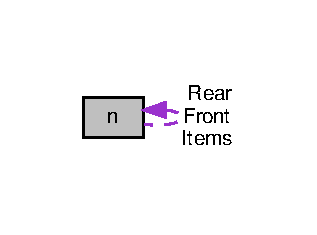
\includegraphics[width=152pt]{df/def/structn__coll__graph}
\end{center}
\end{figure}
\subsection*{Public Attributes}
\begin{DoxyCompactItemize}
\item 
\hyperlink{structn}{n} state\+\_\+cmd \hyperlink{structn_aa86135b44bdda3f39f31e653b9b1d959}{Items} \mbox{[}10\mbox{]}
\item 
\hyperlink{structn}{n} \hyperlink{ab__common_8h_ae9b1af5c037e57a98884758875d3a7c4}{s32} \hyperlink{structn_aac2a7e440b503d7e38c905145522dc4f}{Front}
\item 
\hyperlink{structn}{n} \hyperlink{ab__common_8h_ae9b1af5c037e57a98884758875d3a7c4}{s32} \hyperlink{structn_ab3dbe3587b54eb3d74ed1baf3387d15c}{Rear}
\end{DoxyCompactItemize}


\subsection{Member Data Documentation}
\mbox{\Hypertarget{structn_aac2a7e440b503d7e38c905145522dc4f}\label{structn_aac2a7e440b503d7e38c905145522dc4f}} 
\index{n@{n}!Front@{Front}}
\index{Front@{Front}!n@{n}}
\subsubsection{\texorpdfstring{Front}{Front}}
{\footnotesize\ttfamily \hyperlink{structn}{n} \hyperlink{ab__common_8h_ae9b1af5c037e57a98884758875d3a7c4}{s32} n\+::\+Front}

\mbox{\Hypertarget{structn_aa86135b44bdda3f39f31e653b9b1d959}\label{structn_aa86135b44bdda3f39f31e653b9b1d959}} 
\index{n@{n}!Items@{Items}}
\index{Items@{Items}!n@{n}}
\subsubsection{\texorpdfstring{Items}{Items}}
{\footnotesize\ttfamily \hyperlink{structn}{n} state\+\_\+cmd n\+::\+Items\mbox{[}10\mbox{]}}

\mbox{\Hypertarget{structn_ab3dbe3587b54eb3d74ed1baf3387d15c}\label{structn_ab3dbe3587b54eb3d74ed1baf3387d15c}} 
\index{n@{n}!Rear@{Rear}}
\index{Rear@{Rear}!n@{n}}
\subsubsection{\texorpdfstring{Rear}{Rear}}
{\footnotesize\ttfamily \hyperlink{structn}{n} \hyperlink{ab__common_8h_ae9b1af5c037e57a98884758875d3a7c4}{s32} n\+::\+Rear}



The documentation for this struct was generated from the following file\+:\begin{DoxyCompactItemize}
\item 
\hyperlink{state__template_8cpp}{state\+\_\+template.\+cpp}\end{DoxyCompactItemize}

\hypertarget{structoption}{}\section{option Struct Reference}
\label{structoption}\index{option@{option}}


{\ttfamily \#include $<$gopt.\+h$>$}

\subsection*{Public Attributes}
\begin{DoxyCompactItemize}
\item 
char \hyperlink{structoption_abc0af4c8306684c8c31bb88193a3b040}{short\+\_\+name}
\item 
const char $\ast$ \hyperlink{structoption_afa3bd21f993495477da6350fbdd159da}{long\+\_\+name}
\item 
unsigned int \hyperlink{structoption_a3bb757702735846b5461681fe1af2529}{flags}
\item 
unsigned int \hyperlink{structoption_aca097c2f33b010b53ddaf97a769f432d}{count}
\item 
char $\ast$ \hyperlink{structoption_ac7abe5f58b64ad7ac150d438905b86dd}{argument}
\end{DoxyCompactItemize}


\subsection{Member Data Documentation}
\mbox{\Hypertarget{structoption_ac7abe5f58b64ad7ac150d438905b86dd}\label{structoption_ac7abe5f58b64ad7ac150d438905b86dd}} 
\index{option@{option}!argument@{argument}}
\index{argument@{argument}!option@{option}}
\subsubsection{\texorpdfstring{argument}{argument}}
{\footnotesize\ttfamily char$\ast$ option\+::argument}

\mbox{\Hypertarget{structoption_aca097c2f33b010b53ddaf97a769f432d}\label{structoption_aca097c2f33b010b53ddaf97a769f432d}} 
\index{option@{option}!count@{count}}
\index{count@{count}!option@{option}}
\subsubsection{\texorpdfstring{count}{count}}
{\footnotesize\ttfamily unsigned int option\+::count}

\mbox{\Hypertarget{structoption_a3bb757702735846b5461681fe1af2529}\label{structoption_a3bb757702735846b5461681fe1af2529}} 
\index{option@{option}!flags@{flags}}
\index{flags@{flags}!option@{option}}
\subsubsection{\texorpdfstring{flags}{flags}}
{\footnotesize\ttfamily unsigned int option\+::flags}

\mbox{\Hypertarget{structoption_afa3bd21f993495477da6350fbdd159da}\label{structoption_afa3bd21f993495477da6350fbdd159da}} 
\index{option@{option}!long\+\_\+name@{long\+\_\+name}}
\index{long\+\_\+name@{long\+\_\+name}!option@{option}}
\subsubsection{\texorpdfstring{long\+\_\+name}{long\_name}}
{\footnotesize\ttfamily const char$\ast$ option\+::long\+\_\+name}

\mbox{\Hypertarget{structoption_abc0af4c8306684c8c31bb88193a3b040}\label{structoption_abc0af4c8306684c8c31bb88193a3b040}} 
\index{option@{option}!short\+\_\+name@{short\+\_\+name}}
\index{short\+\_\+name@{short\+\_\+name}!option@{option}}
\subsubsection{\texorpdfstring{short\+\_\+name}{short\_name}}
{\footnotesize\ttfamily char option\+::short\+\_\+name}



The documentation for this struct was generated from the following file\+:\begin{DoxyCompactItemize}
\item 
\hyperlink{gopt_8h}{gopt.\+h}\end{DoxyCompactItemize}

\hypertarget{structoutput__data}{}\section{output\+\_\+data Struct Reference}
\label{structoutput__data}\index{output\+\_\+data@{output\+\_\+data}}


{\ttfamily \#include $<$ab\+\_\+parser.\+h$>$}



Collaboration diagram for output\+\_\+data\+:\nopagebreak
\begin{figure}[H]
\begin{center}
\leavevmode
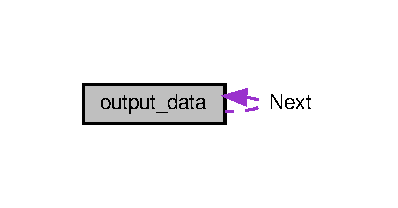
\includegraphics[width=191pt]{dc/d66/structoutput__data__coll__graph}
\end{center}
\end{figure}
\subsection*{Public Attributes}
\begin{DoxyCompactItemize}
\item 
char \hyperlink{structoutput__data_a4b5cddf8fc02cfb5219eafd71e3b3645}{Output\+String} \mbox{[}\hyperlink{ab__common_8h_a9e89c74d1fedd0a954107d7ab01481cc}{Kilobytes}(200)\mbox{]}
\item 
size\+\_\+t \hyperlink{structoutput__data_ac960304f0c5df1d42068abe8bb6a362a}{Used}
\item 
\hyperlink{structoutput__data}{output\+\_\+data} $\ast$ \hyperlink{structoutput__data_ab48e74baa16f37fe4f5b87faed472657}{Next}
\end{DoxyCompactItemize}


\subsection{Member Data Documentation}
\mbox{\Hypertarget{structoutput__data_ab48e74baa16f37fe4f5b87faed472657}\label{structoutput__data_ab48e74baa16f37fe4f5b87faed472657}} 
\index{output\+\_\+data@{output\+\_\+data}!Next@{Next}}
\index{Next@{Next}!output\+\_\+data@{output\+\_\+data}}
\subsubsection{\texorpdfstring{Next}{Next}}
{\footnotesize\ttfamily \hyperlink{structoutput__data}{output\+\_\+data}$\ast$ output\+\_\+data\+::\+Next}

\mbox{\Hypertarget{structoutput__data_a4b5cddf8fc02cfb5219eafd71e3b3645}\label{structoutput__data_a4b5cddf8fc02cfb5219eafd71e3b3645}} 
\index{output\+\_\+data@{output\+\_\+data}!Output\+String@{Output\+String}}
\index{Output\+String@{Output\+String}!output\+\_\+data@{output\+\_\+data}}
\subsubsection{\texorpdfstring{Output\+String}{OutputString}}
{\footnotesize\ttfamily char output\+\_\+data\+::\+Output\+String\mbox{[}\hyperlink{ab__common_8h_a9e89c74d1fedd0a954107d7ab01481cc}{Kilobytes}(200)\mbox{]}}

\mbox{\Hypertarget{structoutput__data_ac960304f0c5df1d42068abe8bb6a362a}\label{structoutput__data_ac960304f0c5df1d42068abe8bb6a362a}} 
\index{output\+\_\+data@{output\+\_\+data}!Used@{Used}}
\index{Used@{Used}!output\+\_\+data@{output\+\_\+data}}
\subsubsection{\texorpdfstring{Used}{Used}}
{\footnotesize\ttfamily size\+\_\+t output\+\_\+data\+::\+Used}



The documentation for this struct was generated from the following file\+:\begin{DoxyCompactItemize}
\item 
\hyperlink{ab__parser_8h}{ab\+\_\+parser.\+h}\end{DoxyCompactItemize}

\hypertarget{structparser}{}\section{parser Struct Reference}
\label{structparser}\index{parser@{parser}}


{\ttfamily \#include $<$ab\+\_\+parser.\+h$>$}



Collaboration diagram for parser\+:\nopagebreak
\begin{figure}[H]
\begin{center}
\leavevmode
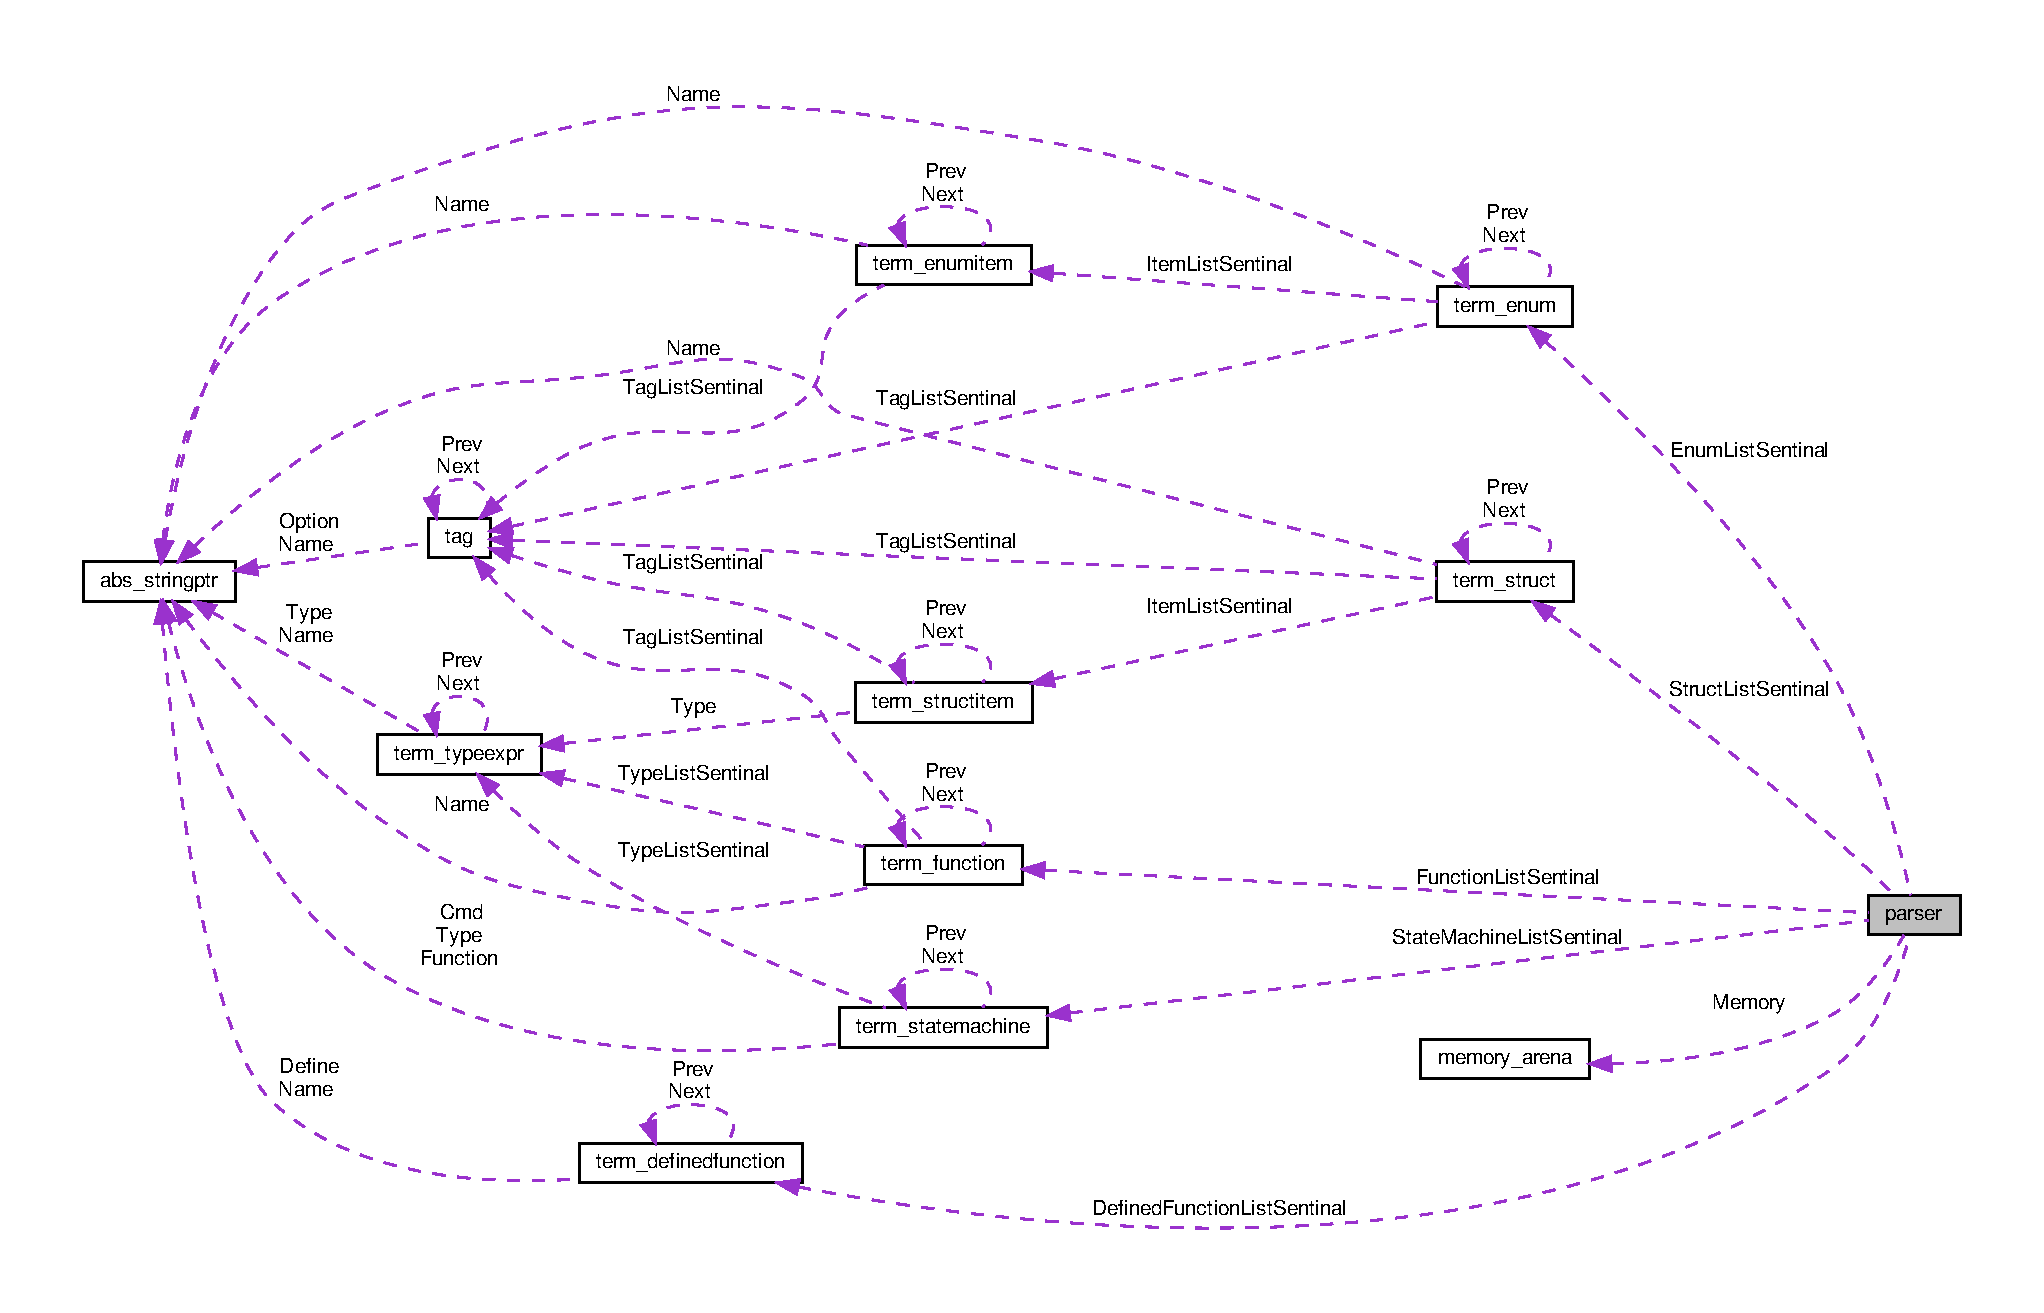
\includegraphics[width=350pt]{d1/d68/structparser__coll__graph}
\end{center}
\end{figure}
\subsection*{Public Attributes}
\begin{DoxyCompactItemize}
\item 
\hyperlink{structmemory__arena}{memory\+\_\+arena} $\ast$ \hyperlink{structparser_ae92434364d983495b64df17550f40d27}{Memory}
\item 
\hyperlink{structterm__struct}{term\+\_\+struct} \hyperlink{structparser_accfacf760af582468d591a06259406be}{Struct\+List\+Sentinal}
\item 
\hyperlink{structterm__enum}{term\+\_\+enum} \hyperlink{structparser_a8023ac3e70ded1ba71e6a2974a9e22b6}{Enum\+List\+Sentinal}
\item 
\hyperlink{structterm__function}{term\+\_\+function} \hyperlink{structparser_a43e51e28e997b7acf6121eb6e6a894f1}{Function\+List\+Sentinal}
\item 
\hyperlink{structterm__statemachine}{term\+\_\+statemachine} \hyperlink{structparser_aa29d6dda9d3d933604823ec27584f162}{State\+Machine\+List\+Sentinal}
\item 
\hyperlink{structterm__definedfunction}{term\+\_\+definedfunction} \hyperlink{structparser_a536dbd6d3a451a05b2365772bd5533a5}{Defined\+Function\+List\+Sentinal}
\end{DoxyCompactItemize}


\subsection{Member Data Documentation}
\mbox{\Hypertarget{structparser_a536dbd6d3a451a05b2365772bd5533a5}\label{structparser_a536dbd6d3a451a05b2365772bd5533a5}} 
\index{parser@{parser}!Defined\+Function\+List\+Sentinal@{Defined\+Function\+List\+Sentinal}}
\index{Defined\+Function\+List\+Sentinal@{Defined\+Function\+List\+Sentinal}!parser@{parser}}
\subsubsection{\texorpdfstring{Defined\+Function\+List\+Sentinal}{DefinedFunctionListSentinal}}
{\footnotesize\ttfamily \hyperlink{structterm__definedfunction}{term\+\_\+definedfunction} parser\+::\+Defined\+Function\+List\+Sentinal}

\mbox{\Hypertarget{structparser_a8023ac3e70ded1ba71e6a2974a9e22b6}\label{structparser_a8023ac3e70ded1ba71e6a2974a9e22b6}} 
\index{parser@{parser}!Enum\+List\+Sentinal@{Enum\+List\+Sentinal}}
\index{Enum\+List\+Sentinal@{Enum\+List\+Sentinal}!parser@{parser}}
\subsubsection{\texorpdfstring{Enum\+List\+Sentinal}{EnumListSentinal}}
{\footnotesize\ttfamily \hyperlink{structterm__enum}{term\+\_\+enum} parser\+::\+Enum\+List\+Sentinal}

\mbox{\Hypertarget{structparser_a43e51e28e997b7acf6121eb6e6a894f1}\label{structparser_a43e51e28e997b7acf6121eb6e6a894f1}} 
\index{parser@{parser}!Function\+List\+Sentinal@{Function\+List\+Sentinal}}
\index{Function\+List\+Sentinal@{Function\+List\+Sentinal}!parser@{parser}}
\subsubsection{\texorpdfstring{Function\+List\+Sentinal}{FunctionListSentinal}}
{\footnotesize\ttfamily \hyperlink{structterm__function}{term\+\_\+function} parser\+::\+Function\+List\+Sentinal}

\mbox{\Hypertarget{structparser_ae92434364d983495b64df17550f40d27}\label{structparser_ae92434364d983495b64df17550f40d27}} 
\index{parser@{parser}!Memory@{Memory}}
\index{Memory@{Memory}!parser@{parser}}
\subsubsection{\texorpdfstring{Memory}{Memory}}
{\footnotesize\ttfamily \hyperlink{structmemory__arena}{memory\+\_\+arena}$\ast$ parser\+::\+Memory}

\mbox{\Hypertarget{structparser_aa29d6dda9d3d933604823ec27584f162}\label{structparser_aa29d6dda9d3d933604823ec27584f162}} 
\index{parser@{parser}!State\+Machine\+List\+Sentinal@{State\+Machine\+List\+Sentinal}}
\index{State\+Machine\+List\+Sentinal@{State\+Machine\+List\+Sentinal}!parser@{parser}}
\subsubsection{\texorpdfstring{State\+Machine\+List\+Sentinal}{StateMachineListSentinal}}
{\footnotesize\ttfamily \hyperlink{structterm__statemachine}{term\+\_\+statemachine} parser\+::\+State\+Machine\+List\+Sentinal}

\mbox{\Hypertarget{structparser_accfacf760af582468d591a06259406be}\label{structparser_accfacf760af582468d591a06259406be}} 
\index{parser@{parser}!Struct\+List\+Sentinal@{Struct\+List\+Sentinal}}
\index{Struct\+List\+Sentinal@{Struct\+List\+Sentinal}!parser@{parser}}
\subsubsection{\texorpdfstring{Struct\+List\+Sentinal}{StructListSentinal}}
{\footnotesize\ttfamily \hyperlink{structterm__struct}{term\+\_\+struct} parser\+::\+Struct\+List\+Sentinal}



The documentation for this struct was generated from the following file\+:\begin{DoxyCompactItemize}
\item 
\hyperlink{ab__parser_8h}{ab\+\_\+parser.\+h}\end{DoxyCompactItemize}

\hypertarget{structstate2__cmd__queue}{}\section{state2\+\_\+cmd\+\_\+queue Struct Reference}
\label{structstate2__cmd__queue}\index{state2\+\_\+cmd\+\_\+queue@{state2\+\_\+cmd\+\_\+queue}}


{\ttfamily \#include $<$Generated\+Sample.\+h$>$}

\subsection*{Public Attributes}
\begin{DoxyCompactItemize}
\item 
state2\+\_\+cmd \hyperlink{structstate2__cmd__queue_afe743bb71aaae1d2dd528c63b01d1043}{Items} \mbox{[}10\mbox{]}
\item 
\hyperlink{ab__common_8h_ae9b1af5c037e57a98884758875d3a7c4}{s32} \hyperlink{structstate2__cmd__queue_a9b97a95eea73647be7630841ca5f3124}{Front}
\item 
\hyperlink{ab__common_8h_ae9b1af5c037e57a98884758875d3a7c4}{s32} \hyperlink{structstate2__cmd__queue_a3417bc9526018e0f80aafdf292491ab0}{Rear}
\end{DoxyCompactItemize}


\subsection{Member Data Documentation}
\mbox{\Hypertarget{structstate2__cmd__queue_a9b97a95eea73647be7630841ca5f3124}\label{structstate2__cmd__queue_a9b97a95eea73647be7630841ca5f3124}} 
\index{state2\+\_\+cmd\+\_\+queue@{state2\+\_\+cmd\+\_\+queue}!Front@{Front}}
\index{Front@{Front}!state2\+\_\+cmd\+\_\+queue@{state2\+\_\+cmd\+\_\+queue}}
\subsubsection{\texorpdfstring{Front}{Front}}
{\footnotesize\ttfamily \hyperlink{ab__common_8h_ae9b1af5c037e57a98884758875d3a7c4}{s32} state2\+\_\+cmd\+\_\+queue\+::\+Front}

\mbox{\Hypertarget{structstate2__cmd__queue_afe743bb71aaae1d2dd528c63b01d1043}\label{structstate2__cmd__queue_afe743bb71aaae1d2dd528c63b01d1043}} 
\index{state2\+\_\+cmd\+\_\+queue@{state2\+\_\+cmd\+\_\+queue}!Items@{Items}}
\index{Items@{Items}!state2\+\_\+cmd\+\_\+queue@{state2\+\_\+cmd\+\_\+queue}}
\subsubsection{\texorpdfstring{Items}{Items}}
{\footnotesize\ttfamily state2\+\_\+cmd state2\+\_\+cmd\+\_\+queue\+::\+Items}

\mbox{\Hypertarget{structstate2__cmd__queue_a3417bc9526018e0f80aafdf292491ab0}\label{structstate2__cmd__queue_a3417bc9526018e0f80aafdf292491ab0}} 
\index{state2\+\_\+cmd\+\_\+queue@{state2\+\_\+cmd\+\_\+queue}!Rear@{Rear}}
\index{Rear@{Rear}!state2\+\_\+cmd\+\_\+queue@{state2\+\_\+cmd\+\_\+queue}}
\subsubsection{\texorpdfstring{Rear}{Rear}}
{\footnotesize\ttfamily \hyperlink{ab__common_8h_ae9b1af5c037e57a98884758875d3a7c4}{s32} state2\+\_\+cmd\+\_\+queue\+::\+Rear}



The documentation for this struct was generated from the following files\+:\begin{DoxyCompactItemize}
\item 
\hyperlink{GeneratedSample_8h}{Generated\+Sample.\+h}\item 
\hyperlink{test_8h}{test.\+h}\end{DoxyCompactItemize}

\hypertarget{structstate__cmd__queue}{}\section{state\+\_\+cmd\+\_\+queue Struct Reference}
\label{structstate__cmd__queue}\index{state\+\_\+cmd\+\_\+queue@{state\+\_\+cmd\+\_\+queue}}


{\ttfamily \#include $<$Generated\+Sample.\+h$>$}

\subsection*{Public Attributes}
\begin{DoxyCompactItemize}
\item 
state\+\_\+cmd \hyperlink{structstate__cmd__queue_ad2f3220b40d00bfd18621494486b77d2}{Items} \mbox{[}10\mbox{]}
\item 
\hyperlink{ab__common_8h_ae9b1af5c037e57a98884758875d3a7c4}{s32} \hyperlink{structstate__cmd__queue_a55c5a533874f46869f1b0c472dd70a7e}{Front}
\item 
\hyperlink{ab__common_8h_ae9b1af5c037e57a98884758875d3a7c4}{s32} \hyperlink{structstate__cmd__queue_af93455ef4f59c05176a6bd70b07a1f10}{Rear}
\end{DoxyCompactItemize}


\subsection{Member Data Documentation}
\mbox{\Hypertarget{structstate__cmd__queue_a55c5a533874f46869f1b0c472dd70a7e}\label{structstate__cmd__queue_a55c5a533874f46869f1b0c472dd70a7e}} 
\index{state\+\_\+cmd\+\_\+queue@{state\+\_\+cmd\+\_\+queue}!Front@{Front}}
\index{Front@{Front}!state\+\_\+cmd\+\_\+queue@{state\+\_\+cmd\+\_\+queue}}
\subsubsection{\texorpdfstring{Front}{Front}}
{\footnotesize\ttfamily \hyperlink{ab__common_8h_ae9b1af5c037e57a98884758875d3a7c4}{s32} state\+\_\+cmd\+\_\+queue\+::\+Front}

\mbox{\Hypertarget{structstate__cmd__queue_ad2f3220b40d00bfd18621494486b77d2}\label{structstate__cmd__queue_ad2f3220b40d00bfd18621494486b77d2}} 
\index{state\+\_\+cmd\+\_\+queue@{state\+\_\+cmd\+\_\+queue}!Items@{Items}}
\index{Items@{Items}!state\+\_\+cmd\+\_\+queue@{state\+\_\+cmd\+\_\+queue}}
\subsubsection{\texorpdfstring{Items}{Items}}
{\footnotesize\ttfamily state\+\_\+cmd state\+\_\+cmd\+\_\+queue\+::\+Items}

\mbox{\Hypertarget{structstate__cmd__queue_af93455ef4f59c05176a6bd70b07a1f10}\label{structstate__cmd__queue_af93455ef4f59c05176a6bd70b07a1f10}} 
\index{state\+\_\+cmd\+\_\+queue@{state\+\_\+cmd\+\_\+queue}!Rear@{Rear}}
\index{Rear@{Rear}!state\+\_\+cmd\+\_\+queue@{state\+\_\+cmd\+\_\+queue}}
\subsubsection{\texorpdfstring{Rear}{Rear}}
{\footnotesize\ttfamily \hyperlink{ab__common_8h_ae9b1af5c037e57a98884758875d3a7c4}{s32} state\+\_\+cmd\+\_\+queue\+::\+Rear}



The documentation for this struct was generated from the following files\+:\begin{DoxyCompactItemize}
\item 
\hyperlink{GeneratedSample_8h}{Generated\+Sample.\+h}\item 
\hyperlink{test_8h}{test.\+h}\end{DoxyCompactItemize}

\hypertarget{structStruct1}{}\section{Struct1 Struct Reference}
\label{structStruct1}\index{Struct1@{Struct1}}


{\ttfamily \#include $<$Parsed\+C.\+h$>$}

\subsection*{Public Attributes}
\begin{DoxyCompactItemize}
\item 
int \hyperlink{structStruct1_ab81c8013900545021cda963327e1ed73}{S11}
\item 
char \hyperlink{structStruct1_ab5b5ef0442d62f260d3231bfe93f4d3d}{S12}
\item 
long \hyperlink{structStruct1_a2cfde9a801e79d5c1589c5861b52400f}{S13}
\item 
\hyperlink{ParsedC_8h_a542930d5f2f117ff1e21206f2baa51c5}{Enum\+Class1} \hyperlink{structStruct1_afddb16c0b88164bd8aa20988ed456111}{S14}
\item 
\hyperlink{ParsedC_8h_a51df612b239afb50004d7a39b20a5745}{Enum\+Class2} \hyperlink{structStruct1_ae2f5a2f538ffd72951049d7f1a823c37}{S15}
\item 
Some\+Struct \hyperlink{structStruct1_a3b6b2444b54b42fe87aedcada8bfecfb}{S16}
\item 
Some\+Struct $\ast$ \hyperlink{structStruct1_a0b1fc8567906ca443688e94d01589064}{S17}
\item 
char const  $\ast$ \hyperlink{structStruct1_aca681fbabd712288a75280ae511e3fc1}{S18}
\item 
const char $\ast$ \hyperlink{structStruct1_a31b80270ff0d1a01aad2c27a4a55377e}{S19}
\item 
char \hyperlink{structStruct1_a67451c56b7de613f0cbc5834854e04e4}{S1A} \mbox{[}10\mbox{]}
\item 
char $\ast$ \hyperlink{structStruct1_a7275b7b9103247c4731f8f849bbd3cc2}{S1B} \mbox{[}10\mbox{]}
\item 
char const  $\ast$ \hyperlink{structStruct1_a861259f7512616e2a7603ab735c7f5c0}{S1C} \mbox{[}10\mbox{]}
\end{DoxyCompactItemize}


\subsection{Member Data Documentation}
\mbox{\Hypertarget{structStruct1_ab81c8013900545021cda963327e1ed73}\label{structStruct1_ab81c8013900545021cda963327e1ed73}} 
\index{Struct1@{Struct1}!S11@{S11}}
\index{S11@{S11}!Struct1@{Struct1}}
\subsubsection{\texorpdfstring{S11}{S11}}
{\footnotesize\ttfamily int Struct1\+::\+S11}

\mbox{\Hypertarget{structStruct1_ab5b5ef0442d62f260d3231bfe93f4d3d}\label{structStruct1_ab5b5ef0442d62f260d3231bfe93f4d3d}} 
\index{Struct1@{Struct1}!S12@{S12}}
\index{S12@{S12}!Struct1@{Struct1}}
\subsubsection{\texorpdfstring{S12}{S12}}
{\footnotesize\ttfamily char Struct1\+::\+S12}

\mbox{\Hypertarget{structStruct1_a2cfde9a801e79d5c1589c5861b52400f}\label{structStruct1_a2cfde9a801e79d5c1589c5861b52400f}} 
\index{Struct1@{Struct1}!S13@{S13}}
\index{S13@{S13}!Struct1@{Struct1}}
\subsubsection{\texorpdfstring{S13}{S13}}
{\footnotesize\ttfamily long Struct1\+::\+S13}

\mbox{\Hypertarget{structStruct1_afddb16c0b88164bd8aa20988ed456111}\label{structStruct1_afddb16c0b88164bd8aa20988ed456111}} 
\index{Struct1@{Struct1}!S14@{S14}}
\index{S14@{S14}!Struct1@{Struct1}}
\subsubsection{\texorpdfstring{S14}{S14}}
{\footnotesize\ttfamily \hyperlink{ParsedC_8h_a542930d5f2f117ff1e21206f2baa51c5}{Enum\+Class1} Struct1\+::\+S14}

\mbox{\Hypertarget{structStruct1_ae2f5a2f538ffd72951049d7f1a823c37}\label{structStruct1_ae2f5a2f538ffd72951049d7f1a823c37}} 
\index{Struct1@{Struct1}!S15@{S15}}
\index{S15@{S15}!Struct1@{Struct1}}
\subsubsection{\texorpdfstring{S15}{S15}}
{\footnotesize\ttfamily \hyperlink{ParsedC_8h_a51df612b239afb50004d7a39b20a5745}{Enum\+Class2} Struct1\+::\+S15}

\mbox{\Hypertarget{structStruct1_a3b6b2444b54b42fe87aedcada8bfecfb}\label{structStruct1_a3b6b2444b54b42fe87aedcada8bfecfb}} 
\index{Struct1@{Struct1}!S16@{S16}}
\index{S16@{S16}!Struct1@{Struct1}}
\subsubsection{\texorpdfstring{S16}{S16}}
{\footnotesize\ttfamily Some\+Struct Struct1\+::\+S16}

\mbox{\Hypertarget{structStruct1_a0b1fc8567906ca443688e94d01589064}\label{structStruct1_a0b1fc8567906ca443688e94d01589064}} 
\index{Struct1@{Struct1}!S17@{S17}}
\index{S17@{S17}!Struct1@{Struct1}}
\subsubsection{\texorpdfstring{S17}{S17}}
{\footnotesize\ttfamily Some\+Struct$\ast$ Struct1\+::\+S17}

\mbox{\Hypertarget{structStruct1_aca681fbabd712288a75280ae511e3fc1}\label{structStruct1_aca681fbabd712288a75280ae511e3fc1}} 
\index{Struct1@{Struct1}!S18@{S18}}
\index{S18@{S18}!Struct1@{Struct1}}
\subsubsection{\texorpdfstring{S18}{S18}}
{\footnotesize\ttfamily char const$\ast$ Struct1\+::\+S18}

\mbox{\Hypertarget{structStruct1_a31b80270ff0d1a01aad2c27a4a55377e}\label{structStruct1_a31b80270ff0d1a01aad2c27a4a55377e}} 
\index{Struct1@{Struct1}!S19@{S19}}
\index{S19@{S19}!Struct1@{Struct1}}
\subsubsection{\texorpdfstring{S19}{S19}}
{\footnotesize\ttfamily const char$\ast$ Struct1\+::\+S19}

\mbox{\Hypertarget{structStruct1_a67451c56b7de613f0cbc5834854e04e4}\label{structStruct1_a67451c56b7de613f0cbc5834854e04e4}} 
\index{Struct1@{Struct1}!S1A@{S1A}}
\index{S1A@{S1A}!Struct1@{Struct1}}
\subsubsection{\texorpdfstring{S1A}{S1A}}
{\footnotesize\ttfamily char Struct1\+::\+S1A\mbox{[}10\mbox{]}}

\mbox{\Hypertarget{structStruct1_a7275b7b9103247c4731f8f849bbd3cc2}\label{structStruct1_a7275b7b9103247c4731f8f849bbd3cc2}} 
\index{Struct1@{Struct1}!S1B@{S1B}}
\index{S1B@{S1B}!Struct1@{Struct1}}
\subsubsection{\texorpdfstring{S1B}{S1B}}
{\footnotesize\ttfamily char$\ast$ Struct1\+::\+S1B\mbox{[}10\mbox{]}}

\mbox{\Hypertarget{structStruct1_a861259f7512616e2a7603ab735c7f5c0}\label{structStruct1_a861259f7512616e2a7603ab735c7f5c0}} 
\index{Struct1@{Struct1}!S1C@{S1C}}
\index{S1C@{S1C}!Struct1@{Struct1}}
\subsubsection{\texorpdfstring{S1C}{S1C}}
{\footnotesize\ttfamily char const$\ast$ Struct1\+::\+S1C\mbox{[}10\mbox{]}}



The documentation for this struct was generated from the following file\+:\begin{DoxyCompactItemize}
\item 
\hyperlink{ParsedC_8h}{Parsed\+C.\+h}\end{DoxyCompactItemize}

\hypertarget{structStruct1__existlist}{}\section{Struct1\+\_\+existlist Struct Reference}
\label{structStruct1__existlist}\index{Struct1\+\_\+existlist@{Struct1\+\_\+existlist}}


{\ttfamily \#include $<$Generated\+Sample.\+h$>$}

\subsection*{Public Attributes}
\begin{DoxyCompactItemize}
\item 
\hyperlink{ab__common_8h_a70e369648385b50f2d0588e8e8745275}{b8} \hyperlink{structStruct1__existlist_aa61b4cc419870281d6a1639db07dcbce}{S11}
\item 
\hyperlink{ab__common_8h_a70e369648385b50f2d0588e8e8745275}{b8} \hyperlink{structStruct1__existlist_a0acdbd7097744dd1c99f7bd0bd50b2eb}{S12}
\item 
\hyperlink{ab__common_8h_a70e369648385b50f2d0588e8e8745275}{b8} \hyperlink{structStruct1__existlist_ad58fec6927bad277f35e13a4c71b7db3}{S13}
\item 
\hyperlink{ab__common_8h_a70e369648385b50f2d0588e8e8745275}{b8} \hyperlink{structStruct1__existlist_ac0a0d2dd6866e584523d6aa52190e442}{S14}
\item 
\hyperlink{ab__common_8h_a70e369648385b50f2d0588e8e8745275}{b8} \hyperlink{structStruct1__existlist_a9abfba7ee78d15e14a4248ed4fedcfeb}{S15}
\item 
\hyperlink{ab__common_8h_a70e369648385b50f2d0588e8e8745275}{b8} \hyperlink{structStruct1__existlist_a997efd967c6b5e13c65358e6c29ec179}{S16}
\item 
\hyperlink{ab__common_8h_a70e369648385b50f2d0588e8e8745275}{b8} \hyperlink{structStruct1__existlist_afb44ba312d31074f7880f79784924f56}{S17}
\item 
\hyperlink{ab__common_8h_a70e369648385b50f2d0588e8e8745275}{b8} \hyperlink{structStruct1__existlist_acb455a93fe6fecd16ccc16a097d6de7d}{S18}
\item 
\hyperlink{ab__common_8h_a70e369648385b50f2d0588e8e8745275}{b8} \hyperlink{structStruct1__existlist_aef301f5d75575771e444965cb88df1c9}{S19}
\item 
\hyperlink{ab__common_8h_a70e369648385b50f2d0588e8e8745275}{b8} \hyperlink{structStruct1__existlist_a7f046abe604d113d70a4dd771a070dab}{S1A}
\item 
\hyperlink{ab__common_8h_a70e369648385b50f2d0588e8e8745275}{b8} \hyperlink{structStruct1__existlist_a9ff78445079c047dae43b4dedbfaee8f}{S1B}
\item 
\hyperlink{ab__common_8h_a70e369648385b50f2d0588e8e8745275}{b8} \hyperlink{structStruct1__existlist_a51481020415f093e99369044246b67dd}{S1C}
\end{DoxyCompactItemize}


\subsection{Member Data Documentation}
\mbox{\Hypertarget{structStruct1__existlist_aa61b4cc419870281d6a1639db07dcbce}\label{structStruct1__existlist_aa61b4cc419870281d6a1639db07dcbce}} 
\index{Struct1\+\_\+existlist@{Struct1\+\_\+existlist}!S11@{S11}}
\index{S11@{S11}!Struct1\+\_\+existlist@{Struct1\+\_\+existlist}}
\subsubsection{\texorpdfstring{S11}{S11}}
{\footnotesize\ttfamily \hyperlink{ab__common_8h_a70e369648385b50f2d0588e8e8745275}{b8} Struct1\+\_\+existlist\+::\+S11}

\mbox{\Hypertarget{structStruct1__existlist_a0acdbd7097744dd1c99f7bd0bd50b2eb}\label{structStruct1__existlist_a0acdbd7097744dd1c99f7bd0bd50b2eb}} 
\index{Struct1\+\_\+existlist@{Struct1\+\_\+existlist}!S12@{S12}}
\index{S12@{S12}!Struct1\+\_\+existlist@{Struct1\+\_\+existlist}}
\subsubsection{\texorpdfstring{S12}{S12}}
{\footnotesize\ttfamily \hyperlink{ab__common_8h_a70e369648385b50f2d0588e8e8745275}{b8} Struct1\+\_\+existlist\+::\+S12}

\mbox{\Hypertarget{structStruct1__existlist_ad58fec6927bad277f35e13a4c71b7db3}\label{structStruct1__existlist_ad58fec6927bad277f35e13a4c71b7db3}} 
\index{Struct1\+\_\+existlist@{Struct1\+\_\+existlist}!S13@{S13}}
\index{S13@{S13}!Struct1\+\_\+existlist@{Struct1\+\_\+existlist}}
\subsubsection{\texorpdfstring{S13}{S13}}
{\footnotesize\ttfamily \hyperlink{ab__common_8h_a70e369648385b50f2d0588e8e8745275}{b8} Struct1\+\_\+existlist\+::\+S13}

\mbox{\Hypertarget{structStruct1__existlist_ac0a0d2dd6866e584523d6aa52190e442}\label{structStruct1__existlist_ac0a0d2dd6866e584523d6aa52190e442}} 
\index{Struct1\+\_\+existlist@{Struct1\+\_\+existlist}!S14@{S14}}
\index{S14@{S14}!Struct1\+\_\+existlist@{Struct1\+\_\+existlist}}
\subsubsection{\texorpdfstring{S14}{S14}}
{\footnotesize\ttfamily \hyperlink{ab__common_8h_a70e369648385b50f2d0588e8e8745275}{b8} Struct1\+\_\+existlist\+::\+S14}

\mbox{\Hypertarget{structStruct1__existlist_a9abfba7ee78d15e14a4248ed4fedcfeb}\label{structStruct1__existlist_a9abfba7ee78d15e14a4248ed4fedcfeb}} 
\index{Struct1\+\_\+existlist@{Struct1\+\_\+existlist}!S15@{S15}}
\index{S15@{S15}!Struct1\+\_\+existlist@{Struct1\+\_\+existlist}}
\subsubsection{\texorpdfstring{S15}{S15}}
{\footnotesize\ttfamily \hyperlink{ab__common_8h_a70e369648385b50f2d0588e8e8745275}{b8} Struct1\+\_\+existlist\+::\+S15}

\mbox{\Hypertarget{structStruct1__existlist_a997efd967c6b5e13c65358e6c29ec179}\label{structStruct1__existlist_a997efd967c6b5e13c65358e6c29ec179}} 
\index{Struct1\+\_\+existlist@{Struct1\+\_\+existlist}!S16@{S16}}
\index{S16@{S16}!Struct1\+\_\+existlist@{Struct1\+\_\+existlist}}
\subsubsection{\texorpdfstring{S16}{S16}}
{\footnotesize\ttfamily \hyperlink{ab__common_8h_a70e369648385b50f2d0588e8e8745275}{b8} Struct1\+\_\+existlist\+::\+S16}

\mbox{\Hypertarget{structStruct1__existlist_afb44ba312d31074f7880f79784924f56}\label{structStruct1__existlist_afb44ba312d31074f7880f79784924f56}} 
\index{Struct1\+\_\+existlist@{Struct1\+\_\+existlist}!S17@{S17}}
\index{S17@{S17}!Struct1\+\_\+existlist@{Struct1\+\_\+existlist}}
\subsubsection{\texorpdfstring{S17}{S17}}
{\footnotesize\ttfamily \hyperlink{ab__common_8h_a70e369648385b50f2d0588e8e8745275}{b8} Struct1\+\_\+existlist\+::\+S17}

\mbox{\Hypertarget{structStruct1__existlist_acb455a93fe6fecd16ccc16a097d6de7d}\label{structStruct1__existlist_acb455a93fe6fecd16ccc16a097d6de7d}} 
\index{Struct1\+\_\+existlist@{Struct1\+\_\+existlist}!S18@{S18}}
\index{S18@{S18}!Struct1\+\_\+existlist@{Struct1\+\_\+existlist}}
\subsubsection{\texorpdfstring{S18}{S18}}
{\footnotesize\ttfamily \hyperlink{ab__common_8h_a70e369648385b50f2d0588e8e8745275}{b8} Struct1\+\_\+existlist\+::\+S18}

\mbox{\Hypertarget{structStruct1__existlist_aef301f5d75575771e444965cb88df1c9}\label{structStruct1__existlist_aef301f5d75575771e444965cb88df1c9}} 
\index{Struct1\+\_\+existlist@{Struct1\+\_\+existlist}!S19@{S19}}
\index{S19@{S19}!Struct1\+\_\+existlist@{Struct1\+\_\+existlist}}
\subsubsection{\texorpdfstring{S19}{S19}}
{\footnotesize\ttfamily \hyperlink{ab__common_8h_a70e369648385b50f2d0588e8e8745275}{b8} Struct1\+\_\+existlist\+::\+S19}

\mbox{\Hypertarget{structStruct1__existlist_a7f046abe604d113d70a4dd771a070dab}\label{structStruct1__existlist_a7f046abe604d113d70a4dd771a070dab}} 
\index{Struct1\+\_\+existlist@{Struct1\+\_\+existlist}!S1A@{S1A}}
\index{S1A@{S1A}!Struct1\+\_\+existlist@{Struct1\+\_\+existlist}}
\subsubsection{\texorpdfstring{S1A}{S1A}}
{\footnotesize\ttfamily \hyperlink{ab__common_8h_a70e369648385b50f2d0588e8e8745275}{b8} Struct1\+\_\+existlist\+::\+S1A}

\mbox{\Hypertarget{structStruct1__existlist_a9ff78445079c047dae43b4dedbfaee8f}\label{structStruct1__existlist_a9ff78445079c047dae43b4dedbfaee8f}} 
\index{Struct1\+\_\+existlist@{Struct1\+\_\+existlist}!S1B@{S1B}}
\index{S1B@{S1B}!Struct1\+\_\+existlist@{Struct1\+\_\+existlist}}
\subsubsection{\texorpdfstring{S1B}{S1B}}
{\footnotesize\ttfamily \hyperlink{ab__common_8h_a70e369648385b50f2d0588e8e8745275}{b8} Struct1\+\_\+existlist\+::\+S1B}

\mbox{\Hypertarget{structStruct1__existlist_a51481020415f093e99369044246b67dd}\label{structStruct1__existlist_a51481020415f093e99369044246b67dd}} 
\index{Struct1\+\_\+existlist@{Struct1\+\_\+existlist}!S1C@{S1C}}
\index{S1C@{S1C}!Struct1\+\_\+existlist@{Struct1\+\_\+existlist}}
\subsubsection{\texorpdfstring{S1C}{S1C}}
{\footnotesize\ttfamily \hyperlink{ab__common_8h_a70e369648385b50f2d0588e8e8745275}{b8} Struct1\+\_\+existlist\+::\+S1C}



The documentation for this struct was generated from the following files\+:\begin{DoxyCompactItemize}
\item 
\hyperlink{GeneratedSample_8h}{Generated\+Sample.\+h}\item 
\hyperlink{test_8h}{test.\+h}\end{DoxyCompactItemize}

\hypertarget{structStruct2}{}\section{Struct2 Struct Reference}
\label{structStruct2}\index{Struct2@{Struct2}}


{\ttfamily \#include $<$Parsed\+C.\+h$>$}

\subsection*{Public Member Functions}
\begin{DoxyCompactItemize}
\item 
\hyperlink{structStruct2_ae6896a66fa6c6f48393847aed8977521}{T\+AG} (Struct\+Item1, Struct\+Item2\+:\+Id, Struct\+Item3\+:\char`\"{}Some String\char`\"{})
\end{DoxyCompactItemize}
\subsection*{Public Attributes}
\begin{DoxyCompactItemize}
\item 
int \hyperlink{structStruct2_ab05c5f39fc72694124f782d656ded3a0}{S21}
\item 
char \hyperlink{structStruct2_af5f7e7a2c7b3372c2fa25f8e823af21e}{S22}
\item 
long \hyperlink{structStruct2_aa36023d5272e4916a86174b83f384abc}{S23}
\item 
\hyperlink{ParsedC_8h_a542930d5f2f117ff1e21206f2baa51c5}{Enum\+Class1} \hyperlink{structStruct2_afbace320147229ed3e2731608153c052}{S24}
\item 
\hyperlink{ParsedC_8h_a51df612b239afb50004d7a39b20a5745}{Enum\+Class2} \hyperlink{structStruct2_abcb5fd48eb7982bb4f6814c36e0071ec}{S25}
\item 
Some\+Struct \hyperlink{structStruct2_aa044d3679db18f7cb109c0e2b647e906}{S26}
\item 
Some\+Struct $\ast$ \hyperlink{structStruct2_a167bbe0c07423ac881f74ec233954dac}{S27}
\item 
char const  $\ast$ \hyperlink{structStruct2_a34ea25fad0eb64f1019b27878ec7a35a}{S28}
\item 
const char $\ast$ \hyperlink{structStruct2_ab7dbe557e331ce158aebc10448e33b60}{S29}
\item 
char \hyperlink{structStruct2_a890b0c7a9c7fe62acc080ef3df9ac424}{S2A} \mbox{[}10\mbox{]}
\item 
char $\ast$ \hyperlink{structStruct2_a2738d564696ad23d5cc3ea0c92726962}{S2B} \mbox{[}200\mbox{]}
\item 
char const  $\ast$ \hyperlink{structStruct2_a33d414ff28068cbcce9a5afcaad7920b}{S2C} \mbox{[}3000\mbox{]}
\end{DoxyCompactItemize}


\subsection{Member Function Documentation}
\mbox{\Hypertarget{structStruct2_ae6896a66fa6c6f48393847aed8977521}\label{structStruct2_ae6896a66fa6c6f48393847aed8977521}} 
\index{Struct2@{Struct2}!T\+AG@{T\+AG}}
\index{T\+AG@{T\+AG}!Struct2@{Struct2}}
\subsubsection{\texorpdfstring{T\+A\+G()}{TAG()}}
{\footnotesize\ttfamily Struct2\+::\+T\+AG (\begin{DoxyParamCaption}\item[{Struct\+Item1}]{,  }\item[{Struct\+Item2\+:\+Id}]{,  }\item[{Struct\+Item3\+:\char`\"{}Some String\char`\"{}}]{ }\end{DoxyParamCaption})}



\subsection{Member Data Documentation}
\mbox{\Hypertarget{structStruct2_ab05c5f39fc72694124f782d656ded3a0}\label{structStruct2_ab05c5f39fc72694124f782d656ded3a0}} 
\index{Struct2@{Struct2}!S21@{S21}}
\index{S21@{S21}!Struct2@{Struct2}}
\subsubsection{\texorpdfstring{S21}{S21}}
{\footnotesize\ttfamily int Struct2\+::\+S21}

\mbox{\Hypertarget{structStruct2_af5f7e7a2c7b3372c2fa25f8e823af21e}\label{structStruct2_af5f7e7a2c7b3372c2fa25f8e823af21e}} 
\index{Struct2@{Struct2}!S22@{S22}}
\index{S22@{S22}!Struct2@{Struct2}}
\subsubsection{\texorpdfstring{S22}{S22}}
{\footnotesize\ttfamily char Struct2\+::\+S22}

\mbox{\Hypertarget{structStruct2_aa36023d5272e4916a86174b83f384abc}\label{structStruct2_aa36023d5272e4916a86174b83f384abc}} 
\index{Struct2@{Struct2}!S23@{S23}}
\index{S23@{S23}!Struct2@{Struct2}}
\subsubsection{\texorpdfstring{S23}{S23}}
{\footnotesize\ttfamily long Struct2\+::\+S23}

\mbox{\Hypertarget{structStruct2_afbace320147229ed3e2731608153c052}\label{structStruct2_afbace320147229ed3e2731608153c052}} 
\index{Struct2@{Struct2}!S24@{S24}}
\index{S24@{S24}!Struct2@{Struct2}}
\subsubsection{\texorpdfstring{S24}{S24}}
{\footnotesize\ttfamily \hyperlink{ParsedC_8h_a542930d5f2f117ff1e21206f2baa51c5}{Enum\+Class1} Struct2\+::\+S24}

\mbox{\Hypertarget{structStruct2_abcb5fd48eb7982bb4f6814c36e0071ec}\label{structStruct2_abcb5fd48eb7982bb4f6814c36e0071ec}} 
\index{Struct2@{Struct2}!S25@{S25}}
\index{S25@{S25}!Struct2@{Struct2}}
\subsubsection{\texorpdfstring{S25}{S25}}
{\footnotesize\ttfamily \hyperlink{ParsedC_8h_a51df612b239afb50004d7a39b20a5745}{Enum\+Class2} Struct2\+::\+S25}

\mbox{\Hypertarget{structStruct2_aa044d3679db18f7cb109c0e2b647e906}\label{structStruct2_aa044d3679db18f7cb109c0e2b647e906}} 
\index{Struct2@{Struct2}!S26@{S26}}
\index{S26@{S26}!Struct2@{Struct2}}
\subsubsection{\texorpdfstring{S26}{S26}}
{\footnotesize\ttfamily Some\+Struct Struct2\+::\+S26}

\mbox{\Hypertarget{structStruct2_a167bbe0c07423ac881f74ec233954dac}\label{structStruct2_a167bbe0c07423ac881f74ec233954dac}} 
\index{Struct2@{Struct2}!S27@{S27}}
\index{S27@{S27}!Struct2@{Struct2}}
\subsubsection{\texorpdfstring{S27}{S27}}
{\footnotesize\ttfamily Some\+Struct$\ast$ Struct2\+::\+S27}

\mbox{\Hypertarget{structStruct2_a34ea25fad0eb64f1019b27878ec7a35a}\label{structStruct2_a34ea25fad0eb64f1019b27878ec7a35a}} 
\index{Struct2@{Struct2}!S28@{S28}}
\index{S28@{S28}!Struct2@{Struct2}}
\subsubsection{\texorpdfstring{S28}{S28}}
{\footnotesize\ttfamily char const$\ast$ Struct2\+::\+S28}

\mbox{\Hypertarget{structStruct2_ab7dbe557e331ce158aebc10448e33b60}\label{structStruct2_ab7dbe557e331ce158aebc10448e33b60}} 
\index{Struct2@{Struct2}!S29@{S29}}
\index{S29@{S29}!Struct2@{Struct2}}
\subsubsection{\texorpdfstring{S29}{S29}}
{\footnotesize\ttfamily const char$\ast$ Struct2\+::\+S29}

\mbox{\Hypertarget{structStruct2_a890b0c7a9c7fe62acc080ef3df9ac424}\label{structStruct2_a890b0c7a9c7fe62acc080ef3df9ac424}} 
\index{Struct2@{Struct2}!S2A@{S2A}}
\index{S2A@{S2A}!Struct2@{Struct2}}
\subsubsection{\texorpdfstring{S2A}{S2A}}
{\footnotesize\ttfamily char Struct2\+::\+S2A\mbox{[}10\mbox{]}}

\mbox{\Hypertarget{structStruct2_a2738d564696ad23d5cc3ea0c92726962}\label{structStruct2_a2738d564696ad23d5cc3ea0c92726962}} 
\index{Struct2@{Struct2}!S2B@{S2B}}
\index{S2B@{S2B}!Struct2@{Struct2}}
\subsubsection{\texorpdfstring{S2B}{S2B}}
{\footnotesize\ttfamily char$\ast$ Struct2\+::\+S2B\mbox{[}200\mbox{]}}

\mbox{\Hypertarget{structStruct2_a33d414ff28068cbcce9a5afcaad7920b}\label{structStruct2_a33d414ff28068cbcce9a5afcaad7920b}} 
\index{Struct2@{Struct2}!S2C@{S2C}}
\index{S2C@{S2C}!Struct2@{Struct2}}
\subsubsection{\texorpdfstring{S2C}{S2C}}
{\footnotesize\ttfamily char const$\ast$ Struct2\+::\+S2C\mbox{[}3000\mbox{]}}



The documentation for this struct was generated from the following file\+:\begin{DoxyCompactItemize}
\item 
\hyperlink{ParsedC_8h}{Parsed\+C.\+h}\end{DoxyCompactItemize}

\hypertarget{structtag}{}\section{tag Struct Reference}
\label{structtag}\index{tag@{tag}}


{\ttfamily \#include $<$ab\+\_\+parser.\+h$>$}



Collaboration diagram for tag\+:\nopagebreak
\begin{figure}[H]
\begin{center}
\leavevmode
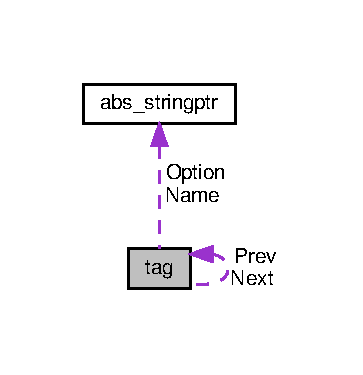
\includegraphics[width=174pt]{db/d25/structtag__coll__graph}
\end{center}
\end{figure}
\subsection*{Public Attributes}
\begin{DoxyCompactItemize}
\item 
\hyperlink{structabs__stringptr}{abs\+\_\+stringptr} \hyperlink{structtag_a4564f437775d5276bcddbc23a6b8881e}{Name}
\item 
\hyperlink{structabs__stringptr}{abs\+\_\+stringptr} \hyperlink{structtag_aa52b4f28c97f8ff006a5fe50d6623a7e}{Option}
\item 
\hyperlink{structtag}{tag} $\ast$ \hyperlink{structtag_ae16f0e5fb461cdbae551134f3e1e8e24}{Next}
\item 
\hyperlink{structtag}{tag} $\ast$ \hyperlink{structtag_af05983b55100a16b3bcd8faad9b50e00}{Prev}
\end{DoxyCompactItemize}


\subsection{Member Data Documentation}
\mbox{\Hypertarget{structtag_a4564f437775d5276bcddbc23a6b8881e}\label{structtag_a4564f437775d5276bcddbc23a6b8881e}} 
\index{tag@{tag}!Name@{Name}}
\index{Name@{Name}!tag@{tag}}
\subsubsection{\texorpdfstring{Name}{Name}}
{\footnotesize\ttfamily \hyperlink{structabs__stringptr}{abs\+\_\+stringptr} tag\+::\+Name}

\mbox{\Hypertarget{structtag_ae16f0e5fb461cdbae551134f3e1e8e24}\label{structtag_ae16f0e5fb461cdbae551134f3e1e8e24}} 
\index{tag@{tag}!Next@{Next}}
\index{Next@{Next}!tag@{tag}}
\subsubsection{\texorpdfstring{Next}{Next}}
{\footnotesize\ttfamily \hyperlink{structtag}{tag}$\ast$ tag\+::\+Next}

\mbox{\Hypertarget{structtag_aa52b4f28c97f8ff006a5fe50d6623a7e}\label{structtag_aa52b4f28c97f8ff006a5fe50d6623a7e}} 
\index{tag@{tag}!Option@{Option}}
\index{Option@{Option}!tag@{tag}}
\subsubsection{\texorpdfstring{Option}{Option}}
{\footnotesize\ttfamily \hyperlink{structabs__stringptr}{abs\+\_\+stringptr} tag\+::\+Option}

\mbox{\Hypertarget{structtag_af05983b55100a16b3bcd8faad9b50e00}\label{structtag_af05983b55100a16b3bcd8faad9b50e00}} 
\index{tag@{tag}!Prev@{Prev}}
\index{Prev@{Prev}!tag@{tag}}
\subsubsection{\texorpdfstring{Prev}{Prev}}
{\footnotesize\ttfamily \hyperlink{structtag}{tag}$\ast$ tag\+::\+Prev}



The documentation for this struct was generated from the following file\+:\begin{DoxyCompactItemize}
\item 
\hyperlink{ab__parser_8h}{ab\+\_\+parser.\+h}\end{DoxyCompactItemize}

\hypertarget{structtemporary__memory}{}\section{temporary\+\_\+memory Struct Reference}
\label{structtemporary__memory}\index{temporary\+\_\+memory@{temporary\+\_\+memory}}


{\ttfamily \#include $<$ab\+\_\+memory.\+h$>$}



Collaboration diagram for temporary\+\_\+memory\+:\nopagebreak
\begin{figure}[H]
\begin{center}
\leavevmode
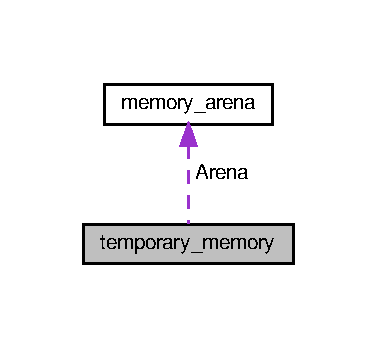
\includegraphics[width=181pt]{db/d58/structtemporary__memory__coll__graph}
\end{center}
\end{figure}
\subsection*{Public Attributes}
\begin{DoxyCompactItemize}
\item 
\hyperlink{structmemory__arena}{memory\+\_\+arena} $\ast$ \hyperlink{structtemporary__memory_abda353234998fedd47ef739e61bddeea}{Arena}
\item 
size\+\_\+t \hyperlink{structtemporary__memory_af2ea8e067d881e044fbecd269e59a556}{Used}
\end{DoxyCompactItemize}


\subsection{Member Data Documentation}
\mbox{\Hypertarget{structtemporary__memory_abda353234998fedd47ef739e61bddeea}\label{structtemporary__memory_abda353234998fedd47ef739e61bddeea}} 
\index{temporary\+\_\+memory@{temporary\+\_\+memory}!Arena@{Arena}}
\index{Arena@{Arena}!temporary\+\_\+memory@{temporary\+\_\+memory}}
\subsubsection{\texorpdfstring{Arena}{Arena}}
{\footnotesize\ttfamily \hyperlink{structmemory__arena}{memory\+\_\+arena}$\ast$ temporary\+\_\+memory\+::\+Arena}

\mbox{\Hypertarget{structtemporary__memory_af2ea8e067d881e044fbecd269e59a556}\label{structtemporary__memory_af2ea8e067d881e044fbecd269e59a556}} 
\index{temporary\+\_\+memory@{temporary\+\_\+memory}!Used@{Used}}
\index{Used@{Used}!temporary\+\_\+memory@{temporary\+\_\+memory}}
\subsubsection{\texorpdfstring{Used}{Used}}
{\footnotesize\ttfamily size\+\_\+t temporary\+\_\+memory\+::\+Used}



The documentation for this struct was generated from the following file\+:\begin{DoxyCompactItemize}
\item 
\hyperlink{ab__memory_8h}{ab\+\_\+memory.\+h}\end{DoxyCompactItemize}

\hypertarget{structterm__definedfunction}{}\doxysection{term\+\_\+definedfunction Struct Reference}
\label{structterm__definedfunction}\index{term\_definedfunction@{term\_definedfunction}}


{\ttfamily \#include $<$ab\+\_\+parser.\+h$>$}



Collaboration diagram for term\+\_\+definedfunction\+:\nopagebreak
\begin{figure}[H]
\begin{center}
\leavevmode
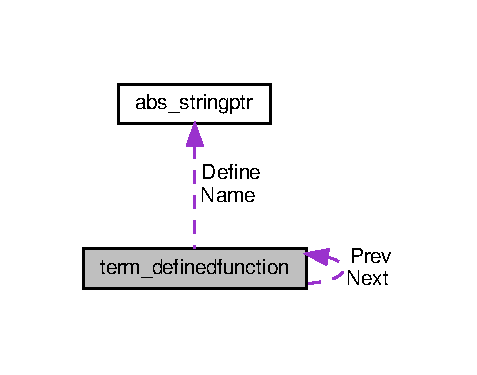
\includegraphics[width=230pt]{df/da2/structterm__definedfunction__coll__graph}
\end{center}
\end{figure}
\doxysubsection*{Public Attributes}
\begin{DoxyCompactItemize}
\item 
st\+\_\+ptr \mbox{\hyperlink{structterm__definedfunction_ad55b79d386e27412ffe321d1543c5a97}{Define}}
\item 
st\+\_\+ptr \mbox{\hyperlink{structterm__definedfunction_a0ca3f3ba52e981e2be9549ea533f7d60}{Name}}
\item 
\mbox{\hyperlink{structterm__definedfunction}{term\+\_\+definedfunction}} $\ast$ \mbox{\hyperlink{structterm__definedfunction_ae4d62f23998fa05c8b5e4e900980460c}{Next}}
\item 
\mbox{\hyperlink{structterm__definedfunction}{term\+\_\+definedfunction}} $\ast$ \mbox{\hyperlink{structterm__definedfunction_a8f3ed1e8ae1fa3012452929ca8cb0da3}{Prev}}
\end{DoxyCompactItemize}


\doxysubsection{Member Data Documentation}
\mbox{\Hypertarget{structterm__definedfunction_ad55b79d386e27412ffe321d1543c5a97}\label{structterm__definedfunction_ad55b79d386e27412ffe321d1543c5a97}} 
\index{term\_definedfunction@{term\_definedfunction}!Define@{Define}}
\index{Define@{Define}!term\_definedfunction@{term\_definedfunction}}
\doxysubsubsection{\texorpdfstring{Define}{Define}}
{\footnotesize\ttfamily st\+\_\+ptr term\+\_\+definedfunction\+::\+Define}

\mbox{\Hypertarget{structterm__definedfunction_a0ca3f3ba52e981e2be9549ea533f7d60}\label{structterm__definedfunction_a0ca3f3ba52e981e2be9549ea533f7d60}} 
\index{term\_definedfunction@{term\_definedfunction}!Name@{Name}}
\index{Name@{Name}!term\_definedfunction@{term\_definedfunction}}
\doxysubsubsection{\texorpdfstring{Name}{Name}}
{\footnotesize\ttfamily st\+\_\+ptr term\+\_\+definedfunction\+::\+Name}

\mbox{\Hypertarget{structterm__definedfunction_ae4d62f23998fa05c8b5e4e900980460c}\label{structterm__definedfunction_ae4d62f23998fa05c8b5e4e900980460c}} 
\index{term\_definedfunction@{term\_definedfunction}!Next@{Next}}
\index{Next@{Next}!term\_definedfunction@{term\_definedfunction}}
\doxysubsubsection{\texorpdfstring{Next}{Next}}
{\footnotesize\ttfamily \mbox{\hyperlink{structterm__definedfunction}{term\+\_\+definedfunction}}$\ast$ term\+\_\+definedfunction\+::\+Next}

\mbox{\Hypertarget{structterm__definedfunction_a8f3ed1e8ae1fa3012452929ca8cb0da3}\label{structterm__definedfunction_a8f3ed1e8ae1fa3012452929ca8cb0da3}} 
\index{term\_definedfunction@{term\_definedfunction}!Prev@{Prev}}
\index{Prev@{Prev}!term\_definedfunction@{term\_definedfunction}}
\doxysubsubsection{\texorpdfstring{Prev}{Prev}}
{\footnotesize\ttfamily \mbox{\hyperlink{structterm__definedfunction}{term\+\_\+definedfunction}}$\ast$ term\+\_\+definedfunction\+::\+Prev}



The documentation for this struct was generated from the following file\+:\begin{DoxyCompactItemize}
\item 
\mbox{\hyperlink{ab__parser_8h}{ab\+\_\+parser.\+h}}\end{DoxyCompactItemize}

\hypertarget{structterm__enum}{}\section{term\+\_\+enum Struct Reference}
\label{structterm__enum}\index{term\+\_\+enum@{term\+\_\+enum}}


{\ttfamily \#include $<$ab\+\_\+parser.\+h$>$}



Collaboration diagram for term\+\_\+enum\+:\nopagebreak
\begin{figure}[H]
\begin{center}
\leavevmode
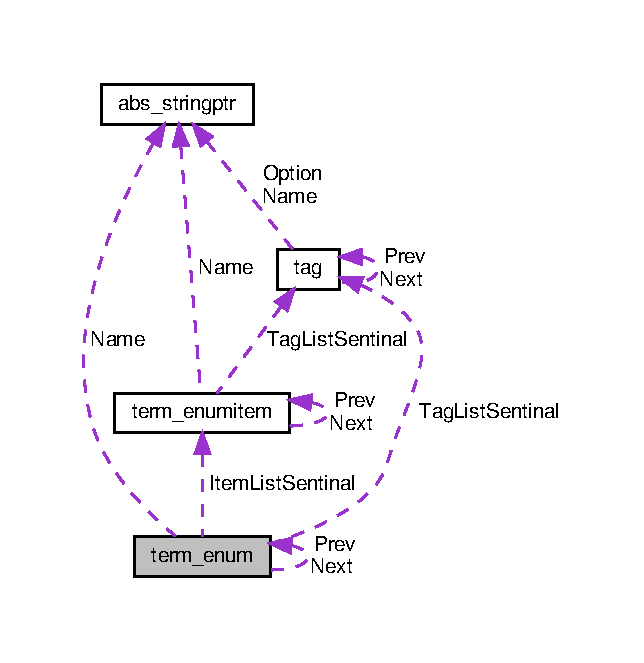
\includegraphics[width=309pt]{d6/d82/structterm__enum__coll__graph}
\end{center}
\end{figure}
\subsection*{Public Attributes}
\begin{DoxyCompactItemize}
\item 
\hyperlink{structabs__stringptr}{abs\+\_\+stringptr} \hyperlink{structterm__enum_a41929255cd1231f08655f7440bd2051f}{Name}
\item 
\hyperlink{structtag}{tag} \hyperlink{structterm__enum_a064766a8666ff84a4571dff4d9a7070a}{Tag\+List\+Sentinal}
\item 
\hyperlink{structterm__enumitem}{term\+\_\+enumitem} \hyperlink{structterm__enum_a982f44fe4692493e3456a80b50805d64}{Item\+List\+Sentinal}
\item 
\hyperlink{ab__common_8h_afaa62991928fb9fb18ff0db62a040aba}{u32} \hyperlink{structterm__enum_a90cb3e473c1ca0a59037e3882af7a1bc}{Item\+Count}
\item 
\hyperlink{structterm__enum}{term\+\_\+enum} $\ast$ \hyperlink{structterm__enum_aa66270184b4f4d6457dda0afd18e25fc}{Next}
\item 
\hyperlink{structterm__enum}{term\+\_\+enum} $\ast$ \hyperlink{structterm__enum_addad4748b3a035a56ed83b5389668f35}{Prev}
\end{DoxyCompactItemize}


\subsection{Member Data Documentation}
\mbox{\Hypertarget{structterm__enum_a90cb3e473c1ca0a59037e3882af7a1bc}\label{structterm__enum_a90cb3e473c1ca0a59037e3882af7a1bc}} 
\index{term\+\_\+enum@{term\+\_\+enum}!Item\+Count@{Item\+Count}}
\index{Item\+Count@{Item\+Count}!term\+\_\+enum@{term\+\_\+enum}}
\subsubsection{\texorpdfstring{Item\+Count}{ItemCount}}
{\footnotesize\ttfamily \hyperlink{ab__common_8h_afaa62991928fb9fb18ff0db62a040aba}{u32} term\+\_\+enum\+::\+Item\+Count}

\mbox{\Hypertarget{structterm__enum_a982f44fe4692493e3456a80b50805d64}\label{structterm__enum_a982f44fe4692493e3456a80b50805d64}} 
\index{term\+\_\+enum@{term\+\_\+enum}!Item\+List\+Sentinal@{Item\+List\+Sentinal}}
\index{Item\+List\+Sentinal@{Item\+List\+Sentinal}!term\+\_\+enum@{term\+\_\+enum}}
\subsubsection{\texorpdfstring{Item\+List\+Sentinal}{ItemListSentinal}}
{\footnotesize\ttfamily \hyperlink{structterm__enumitem}{term\+\_\+enumitem} term\+\_\+enum\+::\+Item\+List\+Sentinal}

\mbox{\Hypertarget{structterm__enum_a41929255cd1231f08655f7440bd2051f}\label{structterm__enum_a41929255cd1231f08655f7440bd2051f}} 
\index{term\+\_\+enum@{term\+\_\+enum}!Name@{Name}}
\index{Name@{Name}!term\+\_\+enum@{term\+\_\+enum}}
\subsubsection{\texorpdfstring{Name}{Name}}
{\footnotesize\ttfamily \hyperlink{structabs__stringptr}{abs\+\_\+stringptr} term\+\_\+enum\+::\+Name}

\mbox{\Hypertarget{structterm__enum_aa66270184b4f4d6457dda0afd18e25fc}\label{structterm__enum_aa66270184b4f4d6457dda0afd18e25fc}} 
\index{term\+\_\+enum@{term\+\_\+enum}!Next@{Next}}
\index{Next@{Next}!term\+\_\+enum@{term\+\_\+enum}}
\subsubsection{\texorpdfstring{Next}{Next}}
{\footnotesize\ttfamily \hyperlink{structterm__enum}{term\+\_\+enum}$\ast$ term\+\_\+enum\+::\+Next}

\mbox{\Hypertarget{structterm__enum_addad4748b3a035a56ed83b5389668f35}\label{structterm__enum_addad4748b3a035a56ed83b5389668f35}} 
\index{term\+\_\+enum@{term\+\_\+enum}!Prev@{Prev}}
\index{Prev@{Prev}!term\+\_\+enum@{term\+\_\+enum}}
\subsubsection{\texorpdfstring{Prev}{Prev}}
{\footnotesize\ttfamily \hyperlink{structterm__enum}{term\+\_\+enum}$\ast$ term\+\_\+enum\+::\+Prev}

\mbox{\Hypertarget{structterm__enum_a064766a8666ff84a4571dff4d9a7070a}\label{structterm__enum_a064766a8666ff84a4571dff4d9a7070a}} 
\index{term\+\_\+enum@{term\+\_\+enum}!Tag\+List\+Sentinal@{Tag\+List\+Sentinal}}
\index{Tag\+List\+Sentinal@{Tag\+List\+Sentinal}!term\+\_\+enum@{term\+\_\+enum}}
\subsubsection{\texorpdfstring{Tag\+List\+Sentinal}{TagListSentinal}}
{\footnotesize\ttfamily \hyperlink{structtag}{tag} term\+\_\+enum\+::\+Tag\+List\+Sentinal}



The documentation for this struct was generated from the following file\+:\begin{DoxyCompactItemize}
\item 
\hyperlink{ab__parser_8h}{ab\+\_\+parser.\+h}\end{DoxyCompactItemize}

\hypertarget{structterm__enumitem}{}\doxysection{term\+\_\+enumitem Struct Reference}
\label{structterm__enumitem}\index{term\_enumitem@{term\_enumitem}}


{\ttfamily \#include $<$ab\+\_\+parser.\+h$>$}



Collaboration diagram for term\+\_\+enumitem\+:\nopagebreak
\begin{figure}[H]
\begin{center}
\leavevmode
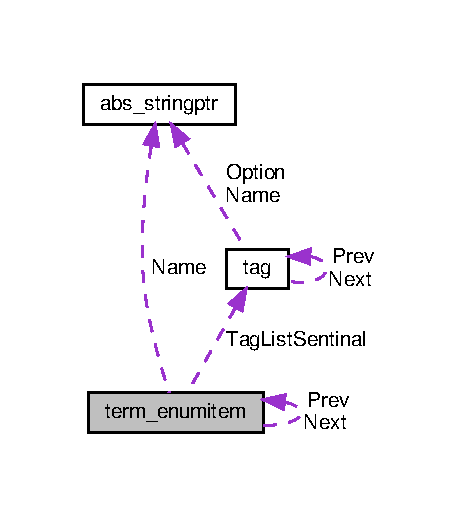
\includegraphics[width=207pt]{dc/def/structterm__enumitem__coll__graph}
\end{center}
\end{figure}
\doxysubsection*{Public Attributes}
\begin{DoxyCompactItemize}
\item 
st\+\_\+ptr \mbox{\hyperlink{structterm__enumitem_a5786103cf50b4967f5901683bfa19625}{Name}}
\item 
\mbox{\hyperlink{structtag}{tag}} \mbox{\hyperlink{structterm__enumitem_ace61cab8da4a090548e03c7a9970deb1}{Tag\+List\+Sentinal}}
\item 
\mbox{\hyperlink{structterm__enumitem}{term\+\_\+enumitem}} $\ast$ \mbox{\hyperlink{structterm__enumitem_a76a5df14c05395f4737800d06c23611a}{Next}}
\item 
\mbox{\hyperlink{structterm__enumitem}{term\+\_\+enumitem}} $\ast$ \mbox{\hyperlink{structterm__enumitem_a9841d521b128ff1d85936bdfded2e425}{Prev}}
\end{DoxyCompactItemize}


\doxysubsection{Member Data Documentation}
\mbox{\Hypertarget{structterm__enumitem_a5786103cf50b4967f5901683bfa19625}\label{structterm__enumitem_a5786103cf50b4967f5901683bfa19625}} 
\index{term\_enumitem@{term\_enumitem}!Name@{Name}}
\index{Name@{Name}!term\_enumitem@{term\_enumitem}}
\doxysubsubsection{\texorpdfstring{Name}{Name}}
{\footnotesize\ttfamily st\+\_\+ptr term\+\_\+enumitem\+::\+Name}

\mbox{\Hypertarget{structterm__enumitem_a76a5df14c05395f4737800d06c23611a}\label{structterm__enumitem_a76a5df14c05395f4737800d06c23611a}} 
\index{term\_enumitem@{term\_enumitem}!Next@{Next}}
\index{Next@{Next}!term\_enumitem@{term\_enumitem}}
\doxysubsubsection{\texorpdfstring{Next}{Next}}
{\footnotesize\ttfamily \mbox{\hyperlink{structterm__enumitem}{term\+\_\+enumitem}}$\ast$ term\+\_\+enumitem\+::\+Next}

\mbox{\Hypertarget{structterm__enumitem_a9841d521b128ff1d85936bdfded2e425}\label{structterm__enumitem_a9841d521b128ff1d85936bdfded2e425}} 
\index{term\_enumitem@{term\_enumitem}!Prev@{Prev}}
\index{Prev@{Prev}!term\_enumitem@{term\_enumitem}}
\doxysubsubsection{\texorpdfstring{Prev}{Prev}}
{\footnotesize\ttfamily \mbox{\hyperlink{structterm__enumitem}{term\+\_\+enumitem}}$\ast$ term\+\_\+enumitem\+::\+Prev}

\mbox{\Hypertarget{structterm__enumitem_ace61cab8da4a090548e03c7a9970deb1}\label{structterm__enumitem_ace61cab8da4a090548e03c7a9970deb1}} 
\index{term\_enumitem@{term\_enumitem}!TagListSentinal@{TagListSentinal}}
\index{TagListSentinal@{TagListSentinal}!term\_enumitem@{term\_enumitem}}
\doxysubsubsection{\texorpdfstring{TagListSentinal}{TagListSentinal}}
{\footnotesize\ttfamily \mbox{\hyperlink{structtag}{tag}} term\+\_\+enumitem\+::\+Tag\+List\+Sentinal}



The documentation for this struct was generated from the following file\+:\begin{DoxyCompactItemize}
\item 
\mbox{\hyperlink{ab__parser_8h}{ab\+\_\+parser.\+h}}\end{DoxyCompactItemize}

\hypertarget{structterm__function}{}\section{term\+\_\+function Struct Reference}
\label{structterm__function}\index{term\+\_\+function@{term\+\_\+function}}


{\ttfamily \#include $<$ab\+\_\+parser.\+h$>$}



Collaboration diagram for term\+\_\+function\+:
\nopagebreak
\begin{figure}[H]
\begin{center}
\leavevmode
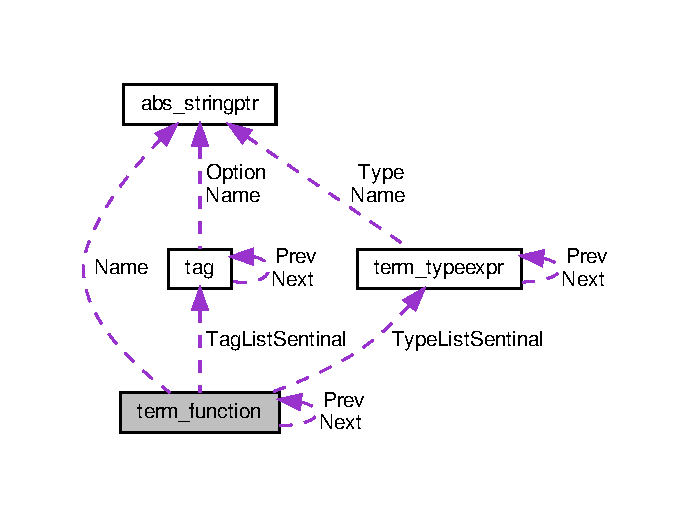
\includegraphics[width=292pt]{d0/dd8/structterm__function__coll__graph}
\end{center}
\end{figure}
\subsection*{Public Attributes}
\begin{DoxyCompactItemize}
\item 
abs\+\_\+stringptr \hyperlink{structterm__function_a44d4f15308d31174ac9443aeefe9544a}{Name}
\item 
\hyperlink{structtag}{tag} \hyperlink{structterm__function_ab3a3bd4264776e6fe2d04b161bd62433}{Tag\+List\+Sentinal}
\item 
\hyperlink{structterm__typeexpr}{term\+\_\+typeexpr} \hyperlink{structterm__function_a96b877553f990184a9da245207de9524}{Type\+List\+Sentinal}
\item 
u32 \hyperlink{structterm__function_a4e47cbfb96047c0ed4e06e87e079fb6a}{Type\+Count}
\item 
\hyperlink{structterm__function}{term\+\_\+function} $\ast$ \hyperlink{structterm__function_a655992a45b7bc18c8208d9a058bb86e6}{Next}
\item 
\hyperlink{structterm__function}{term\+\_\+function} $\ast$ \hyperlink{structterm__function_aab58e6419571c457d2b7563724bed629}{Prev}
\end{DoxyCompactItemize}


\subsection{Member Data Documentation}
\mbox{\Hypertarget{structterm__function_a44d4f15308d31174ac9443aeefe9544a}\label{structterm__function_a44d4f15308d31174ac9443aeefe9544a}} 
\index{term\+\_\+function@{term\+\_\+function}!Name@{Name}}
\index{Name@{Name}!term\+\_\+function@{term\+\_\+function}}
\subsubsection{\texorpdfstring{Name}{Name}}
{\footnotesize\ttfamily abs\+\_\+stringptr term\+\_\+function\+::\+Name}

\mbox{\Hypertarget{structterm__function_a655992a45b7bc18c8208d9a058bb86e6}\label{structterm__function_a655992a45b7bc18c8208d9a058bb86e6}} 
\index{term\+\_\+function@{term\+\_\+function}!Next@{Next}}
\index{Next@{Next}!term\+\_\+function@{term\+\_\+function}}
\subsubsection{\texorpdfstring{Next}{Next}}
{\footnotesize\ttfamily \hyperlink{structterm__function}{term\+\_\+function}$\ast$ term\+\_\+function\+::\+Next}

\mbox{\Hypertarget{structterm__function_aab58e6419571c457d2b7563724bed629}\label{structterm__function_aab58e6419571c457d2b7563724bed629}} 
\index{term\+\_\+function@{term\+\_\+function}!Prev@{Prev}}
\index{Prev@{Prev}!term\+\_\+function@{term\+\_\+function}}
\subsubsection{\texorpdfstring{Prev}{Prev}}
{\footnotesize\ttfamily \hyperlink{structterm__function}{term\+\_\+function}$\ast$ term\+\_\+function\+::\+Prev}

\mbox{\Hypertarget{structterm__function_ab3a3bd4264776e6fe2d04b161bd62433}\label{structterm__function_ab3a3bd4264776e6fe2d04b161bd62433}} 
\index{term\+\_\+function@{term\+\_\+function}!Tag\+List\+Sentinal@{Tag\+List\+Sentinal}}
\index{Tag\+List\+Sentinal@{Tag\+List\+Sentinal}!term\+\_\+function@{term\+\_\+function}}
\subsubsection{\texorpdfstring{Tag\+List\+Sentinal}{TagListSentinal}}
{\footnotesize\ttfamily \hyperlink{structtag}{tag} term\+\_\+function\+::\+Tag\+List\+Sentinal}

\mbox{\Hypertarget{structterm__function_a4e47cbfb96047c0ed4e06e87e079fb6a}\label{structterm__function_a4e47cbfb96047c0ed4e06e87e079fb6a}} 
\index{term\+\_\+function@{term\+\_\+function}!Type\+Count@{Type\+Count}}
\index{Type\+Count@{Type\+Count}!term\+\_\+function@{term\+\_\+function}}
\subsubsection{\texorpdfstring{Type\+Count}{TypeCount}}
{\footnotesize\ttfamily u32 term\+\_\+function\+::\+Type\+Count}

\mbox{\Hypertarget{structterm__function_a96b877553f990184a9da245207de9524}\label{structterm__function_a96b877553f990184a9da245207de9524}} 
\index{term\+\_\+function@{term\+\_\+function}!Type\+List\+Sentinal@{Type\+List\+Sentinal}}
\index{Type\+List\+Sentinal@{Type\+List\+Sentinal}!term\+\_\+function@{term\+\_\+function}}
\subsubsection{\texorpdfstring{Type\+List\+Sentinal}{TypeListSentinal}}
{\footnotesize\ttfamily \hyperlink{structterm__typeexpr}{term\+\_\+typeexpr} term\+\_\+function\+::\+Type\+List\+Sentinal}



The documentation for this struct was generated from the following file\+:\begin{DoxyCompactItemize}
\item 
\hyperlink{ab__parser_8h}{ab\+\_\+parser.\+h}\end{DoxyCompactItemize}

\hypertarget{structterm__statefunction}{}\doxysection{term\+\_\+statefunction Struct Reference}
\label{structterm__statefunction}\index{term\_statefunction@{term\_statefunction}}


{\ttfamily \#include $<$ab\+\_\+parser.\+h$>$}



Collaboration diagram for term\+\_\+statefunction\+:
\nopagebreak
\begin{figure}[H]
\begin{center}
\leavevmode
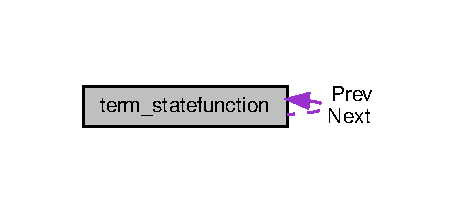
\includegraphics[width=221pt]{dd/d3e/structterm__statefunction__coll__graph}
\end{center}
\end{figure}
\doxysubsection*{Public Attributes}
\begin{DoxyCompactItemize}
\item 
\mbox{\hyperlink{structterm__statefunction}{term\+\_\+statefunction}} $\ast$ \mbox{\hyperlink{structterm__statefunction_a326dae1852433ae2fc11195dd1770ddf}{Next}}
\item 
\mbox{\hyperlink{structterm__statefunction}{term\+\_\+statefunction}} $\ast$ \mbox{\hyperlink{structterm__statefunction_a2693cbcd59a8a1eea7cbc1f8a61efc83}{Prev}}
\end{DoxyCompactItemize}


\doxysubsection{Member Data Documentation}
\mbox{\Hypertarget{structterm__statefunction_a326dae1852433ae2fc11195dd1770ddf}\label{structterm__statefunction_a326dae1852433ae2fc11195dd1770ddf}} 
\index{term\_statefunction@{term\_statefunction}!Next@{Next}}
\index{Next@{Next}!term\_statefunction@{term\_statefunction}}
\doxysubsubsection{\texorpdfstring{Next}{Next}}
{\footnotesize\ttfamily \mbox{\hyperlink{structterm__statefunction}{term\+\_\+statefunction}}$\ast$ term\+\_\+statefunction\+::\+Next}

\mbox{\Hypertarget{structterm__statefunction_a2693cbcd59a8a1eea7cbc1f8a61efc83}\label{structterm__statefunction_a2693cbcd59a8a1eea7cbc1f8a61efc83}} 
\index{term\_statefunction@{term\_statefunction}!Prev@{Prev}}
\index{Prev@{Prev}!term\_statefunction@{term\_statefunction}}
\doxysubsubsection{\texorpdfstring{Prev}{Prev}}
{\footnotesize\ttfamily \mbox{\hyperlink{structterm__statefunction}{term\+\_\+statefunction}}$\ast$ term\+\_\+statefunction\+::\+Prev}



The documentation for this struct was generated from the following file\+:\begin{DoxyCompactItemize}
\item 
\mbox{\hyperlink{ab__parser_8h}{ab\+\_\+parser.\+h}}\end{DoxyCompactItemize}

\hypertarget{structterm__statemachine}{}\doxysection{term\+\_\+statemachine Struct Reference}
\label{structterm__statemachine}\index{term\_statemachine@{term\_statemachine}}


{\ttfamily \#include $<$ab\+\_\+parser.\+h$>$}



Collaboration diagram for term\+\_\+statemachine\+:\nopagebreak
\begin{figure}[H]
\begin{center}
\leavevmode
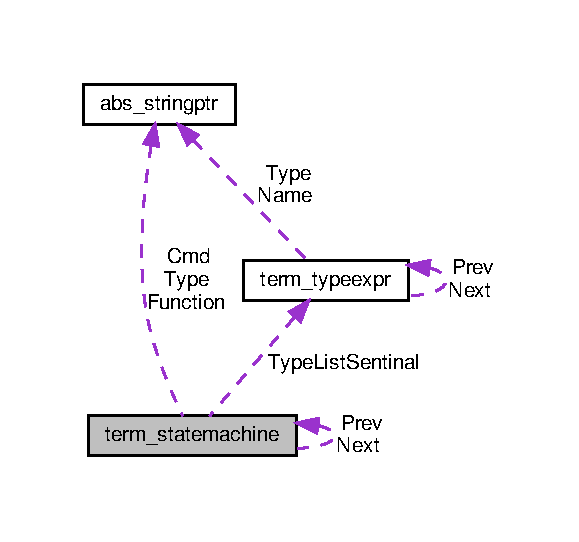
\includegraphics[width=223pt]{de/d7c/structterm__statemachine__coll__graph}
\end{center}
\end{figure}
\doxysubsection*{Public Attributes}
\begin{DoxyCompactItemize}
\item 
st\+\_\+ptr \mbox{\hyperlink{structterm__statemachine_a4c8a27598b9cd9eb13f905ff963ffe24}{Function}}
\item 
st\+\_\+ptr \mbox{\hyperlink{structterm__statemachine_a11af23252a3c9c1a3d7959e905800bae}{Type}}
\item 
st\+\_\+ptr \mbox{\hyperlink{structterm__statemachine_a2f1fc1d8b4b0a816f7ddfe8105a1ce54}{Cmd}}
\item 
\mbox{\hyperlink{structterm__typeexpr}{term\+\_\+typeexpr}} \mbox{\hyperlink{structterm__statemachine_ababd4f7bc69e5ca15fe95a56cdb312af}{Type\+List\+Sentinal}}
\item 
\mbox{\hyperlink{structterm__statemachine}{term\+\_\+statemachine}} $\ast$ \mbox{\hyperlink{structterm__statemachine_a78279e94d1a4f84463c5d7c4fba6bc17}{Next}}
\item 
\mbox{\hyperlink{structterm__statemachine}{term\+\_\+statemachine}} $\ast$ \mbox{\hyperlink{structterm__statemachine_a4e1ec651310e6e0789f9bcb627cfaa70}{Prev}}
\end{DoxyCompactItemize}


\doxysubsection{Member Data Documentation}
\mbox{\Hypertarget{structterm__statemachine_a2f1fc1d8b4b0a816f7ddfe8105a1ce54}\label{structterm__statemachine_a2f1fc1d8b4b0a816f7ddfe8105a1ce54}} 
\index{term\_statemachine@{term\_statemachine}!Cmd@{Cmd}}
\index{Cmd@{Cmd}!term\_statemachine@{term\_statemachine}}
\doxysubsubsection{\texorpdfstring{Cmd}{Cmd}}
{\footnotesize\ttfamily st\+\_\+ptr term\+\_\+statemachine\+::\+Cmd}

\mbox{\Hypertarget{structterm__statemachine_a4c8a27598b9cd9eb13f905ff963ffe24}\label{structterm__statemachine_a4c8a27598b9cd9eb13f905ff963ffe24}} 
\index{term\_statemachine@{term\_statemachine}!Function@{Function}}
\index{Function@{Function}!term\_statemachine@{term\_statemachine}}
\doxysubsubsection{\texorpdfstring{Function}{Function}}
{\footnotesize\ttfamily st\+\_\+ptr term\+\_\+statemachine\+::\+Function}

\mbox{\Hypertarget{structterm__statemachine_a78279e94d1a4f84463c5d7c4fba6bc17}\label{structterm__statemachine_a78279e94d1a4f84463c5d7c4fba6bc17}} 
\index{term\_statemachine@{term\_statemachine}!Next@{Next}}
\index{Next@{Next}!term\_statemachine@{term\_statemachine}}
\doxysubsubsection{\texorpdfstring{Next}{Next}}
{\footnotesize\ttfamily \mbox{\hyperlink{structterm__statemachine}{term\+\_\+statemachine}}$\ast$ term\+\_\+statemachine\+::\+Next}

\mbox{\Hypertarget{structterm__statemachine_a4e1ec651310e6e0789f9bcb627cfaa70}\label{structterm__statemachine_a4e1ec651310e6e0789f9bcb627cfaa70}} 
\index{term\_statemachine@{term\_statemachine}!Prev@{Prev}}
\index{Prev@{Prev}!term\_statemachine@{term\_statemachine}}
\doxysubsubsection{\texorpdfstring{Prev}{Prev}}
{\footnotesize\ttfamily \mbox{\hyperlink{structterm__statemachine}{term\+\_\+statemachine}}$\ast$ term\+\_\+statemachine\+::\+Prev}

\mbox{\Hypertarget{structterm__statemachine_a11af23252a3c9c1a3d7959e905800bae}\label{structterm__statemachine_a11af23252a3c9c1a3d7959e905800bae}} 
\index{term\_statemachine@{term\_statemachine}!Type@{Type}}
\index{Type@{Type}!term\_statemachine@{term\_statemachine}}
\doxysubsubsection{\texorpdfstring{Type}{Type}}
{\footnotesize\ttfamily st\+\_\+ptr term\+\_\+statemachine\+::\+Type}

\mbox{\Hypertarget{structterm__statemachine_ababd4f7bc69e5ca15fe95a56cdb312af}\label{structterm__statemachine_ababd4f7bc69e5ca15fe95a56cdb312af}} 
\index{term\_statemachine@{term\_statemachine}!TypeListSentinal@{TypeListSentinal}}
\index{TypeListSentinal@{TypeListSentinal}!term\_statemachine@{term\_statemachine}}
\doxysubsubsection{\texorpdfstring{TypeListSentinal}{TypeListSentinal}}
{\footnotesize\ttfamily \mbox{\hyperlink{structterm__typeexpr}{term\+\_\+typeexpr}} term\+\_\+statemachine\+::\+Type\+List\+Sentinal}



The documentation for this struct was generated from the following file\+:\begin{DoxyCompactItemize}
\item 
\mbox{\hyperlink{ab__parser_8h}{ab\+\_\+parser.\+h}}\end{DoxyCompactItemize}

\hypertarget{structterm__struct}{}\doxysection{term\+\_\+struct Struct Reference}
\label{structterm__struct}\index{term\_struct@{term\_struct}}


{\ttfamily \#include $<$ab\+\_\+parser.\+h$>$}



Collaboration diagram for term\+\_\+struct\+:
\nopagebreak
\begin{figure}[H]
\begin{center}
\leavevmode
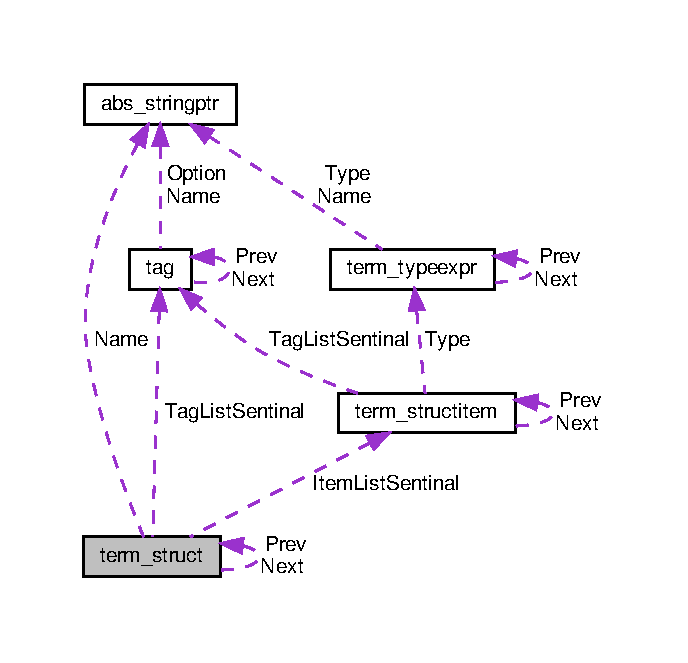
\includegraphics[width=305pt]{df/d72/structterm__struct__coll__graph}
\end{center}
\end{figure}
\doxysubsection*{Public Attributes}
\begin{DoxyCompactItemize}
\item 
abs\+\_\+stringptr \mbox{\hyperlink{structterm__struct_a89d9cb121c9adf97d79fe1a2304c672a}{Name}}
\item 
\mbox{\hyperlink{structtag}{tag}} \mbox{\hyperlink{structterm__struct_a95c474434ab1c1d7e1ac66df37592d68}{Tag\+List\+Sentinal}}
\item 
\mbox{\hyperlink{structterm__structitem}{term\+\_\+structitem}} \mbox{\hyperlink{structterm__struct_a0983a4cdc7024100a2f870b0d484a99d}{Item\+List\+Sentinal}}
\item 
u32 \mbox{\hyperlink{structterm__struct_a7346270cfcb97d2aba636aaccf0a35be}{Item\+Count}}
\item 
\mbox{\hyperlink{structterm__struct}{term\+\_\+struct}} $\ast$ \mbox{\hyperlink{structterm__struct_a733a9fd60e2c6d6dd108fe88e18a8cb8}{Next}}
\item 
\mbox{\hyperlink{structterm__struct}{term\+\_\+struct}} $\ast$ \mbox{\hyperlink{structterm__struct_aa5cc89c03d6af0b5a43680485f5224cb}{Prev}}
\end{DoxyCompactItemize}


\doxysubsection{Member Data Documentation}
\mbox{\Hypertarget{structterm__struct_a7346270cfcb97d2aba636aaccf0a35be}\label{structterm__struct_a7346270cfcb97d2aba636aaccf0a35be}} 
\index{term\_struct@{term\_struct}!ItemCount@{ItemCount}}
\index{ItemCount@{ItemCount}!term\_struct@{term\_struct}}
\doxysubsubsection{\texorpdfstring{ItemCount}{ItemCount}}
{\footnotesize\ttfamily u32 term\+\_\+struct\+::\+Item\+Count}

\mbox{\Hypertarget{structterm__struct_a0983a4cdc7024100a2f870b0d484a99d}\label{structterm__struct_a0983a4cdc7024100a2f870b0d484a99d}} 
\index{term\_struct@{term\_struct}!ItemListSentinal@{ItemListSentinal}}
\index{ItemListSentinal@{ItemListSentinal}!term\_struct@{term\_struct}}
\doxysubsubsection{\texorpdfstring{ItemListSentinal}{ItemListSentinal}}
{\footnotesize\ttfamily \mbox{\hyperlink{structterm__structitem}{term\+\_\+structitem}} term\+\_\+struct\+::\+Item\+List\+Sentinal}

\mbox{\Hypertarget{structterm__struct_a89d9cb121c9adf97d79fe1a2304c672a}\label{structterm__struct_a89d9cb121c9adf97d79fe1a2304c672a}} 
\index{term\_struct@{term\_struct}!Name@{Name}}
\index{Name@{Name}!term\_struct@{term\_struct}}
\doxysubsubsection{\texorpdfstring{Name}{Name}}
{\footnotesize\ttfamily abs\+\_\+stringptr term\+\_\+struct\+::\+Name}

\mbox{\Hypertarget{structterm__struct_a733a9fd60e2c6d6dd108fe88e18a8cb8}\label{structterm__struct_a733a9fd60e2c6d6dd108fe88e18a8cb8}} 
\index{term\_struct@{term\_struct}!Next@{Next}}
\index{Next@{Next}!term\_struct@{term\_struct}}
\doxysubsubsection{\texorpdfstring{Next}{Next}}
{\footnotesize\ttfamily \mbox{\hyperlink{structterm__struct}{term\+\_\+struct}}$\ast$ term\+\_\+struct\+::\+Next}

\mbox{\Hypertarget{structterm__struct_aa5cc89c03d6af0b5a43680485f5224cb}\label{structterm__struct_aa5cc89c03d6af0b5a43680485f5224cb}} 
\index{term\_struct@{term\_struct}!Prev@{Prev}}
\index{Prev@{Prev}!term\_struct@{term\_struct}}
\doxysubsubsection{\texorpdfstring{Prev}{Prev}}
{\footnotesize\ttfamily \mbox{\hyperlink{structterm__struct}{term\+\_\+struct}}$\ast$ term\+\_\+struct\+::\+Prev}

\mbox{\Hypertarget{structterm__struct_a95c474434ab1c1d7e1ac66df37592d68}\label{structterm__struct_a95c474434ab1c1d7e1ac66df37592d68}} 
\index{term\_struct@{term\_struct}!TagListSentinal@{TagListSentinal}}
\index{TagListSentinal@{TagListSentinal}!term\_struct@{term\_struct}}
\doxysubsubsection{\texorpdfstring{TagListSentinal}{TagListSentinal}}
{\footnotesize\ttfamily \mbox{\hyperlink{structtag}{tag}} term\+\_\+struct\+::\+Tag\+List\+Sentinal}



The documentation for this struct was generated from the following file\+:\begin{DoxyCompactItemize}
\item 
\mbox{\hyperlink{ab__parser_8h}{ab\+\_\+parser.\+h}}\end{DoxyCompactItemize}

\hypertarget{structterm__structitem}{}\doxysection{term\+\_\+structitem Struct Reference}
\label{structterm__structitem}\index{term\_structitem@{term\_structitem}}


{\ttfamily \#include $<$ab\+\_\+parser.\+h$>$}



Collaboration diagram for term\+\_\+structitem\+:
\nopagebreak
\begin{figure}[H]
\begin{center}
\leavevmode
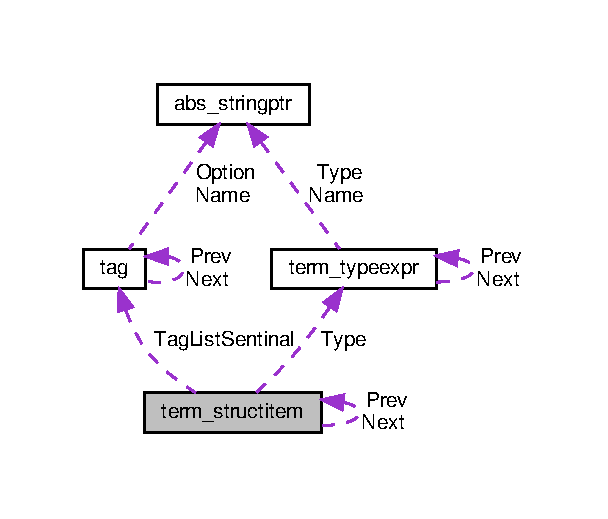
\includegraphics[width=294pt]{df/d30/structterm__structitem__coll__graph}
\end{center}
\end{figure}
\doxysubsection*{Public Attributes}
\begin{DoxyCompactItemize}
\item 
\mbox{\hyperlink{structterm__typeexpr}{term\+\_\+typeexpr}} $\ast$ \mbox{\hyperlink{structterm__structitem_ac2a7c2261f1714cedb33376eb440e66c}{Type}}
\item 
\mbox{\hyperlink{structtag}{tag}} \mbox{\hyperlink{structterm__structitem_a25c03f6130b24c035dadd65fbe5f0110}{Tag\+List\+Sentinal}}
\item 
\mbox{\hyperlink{structterm__structitem}{term\+\_\+structitem}} $\ast$ \mbox{\hyperlink{structterm__structitem_a92becd37fab5b7e4b326e3111c6a7c40}{Next}}
\item 
\mbox{\hyperlink{structterm__structitem}{term\+\_\+structitem}} $\ast$ \mbox{\hyperlink{structterm__structitem_a724d81ad66a76f54b153a97a8b175b7d}{Prev}}
\end{DoxyCompactItemize}


\doxysubsection{Member Data Documentation}
\mbox{\Hypertarget{structterm__structitem_a92becd37fab5b7e4b326e3111c6a7c40}\label{structterm__structitem_a92becd37fab5b7e4b326e3111c6a7c40}} 
\index{term\_structitem@{term\_structitem}!Next@{Next}}
\index{Next@{Next}!term\_structitem@{term\_structitem}}
\doxysubsubsection{\texorpdfstring{Next}{Next}}
{\footnotesize\ttfamily \mbox{\hyperlink{structterm__structitem}{term\+\_\+structitem}}$\ast$ term\+\_\+structitem\+::\+Next}

\mbox{\Hypertarget{structterm__structitem_a724d81ad66a76f54b153a97a8b175b7d}\label{structterm__structitem_a724d81ad66a76f54b153a97a8b175b7d}} 
\index{term\_structitem@{term\_structitem}!Prev@{Prev}}
\index{Prev@{Prev}!term\_structitem@{term\_structitem}}
\doxysubsubsection{\texorpdfstring{Prev}{Prev}}
{\footnotesize\ttfamily \mbox{\hyperlink{structterm__structitem}{term\+\_\+structitem}}$\ast$ term\+\_\+structitem\+::\+Prev}

\mbox{\Hypertarget{structterm__structitem_a25c03f6130b24c035dadd65fbe5f0110}\label{structterm__structitem_a25c03f6130b24c035dadd65fbe5f0110}} 
\index{term\_structitem@{term\_structitem}!TagListSentinal@{TagListSentinal}}
\index{TagListSentinal@{TagListSentinal}!term\_structitem@{term\_structitem}}
\doxysubsubsection{\texorpdfstring{TagListSentinal}{TagListSentinal}}
{\footnotesize\ttfamily \mbox{\hyperlink{structtag}{tag}} term\+\_\+structitem\+::\+Tag\+List\+Sentinal}

\mbox{\Hypertarget{structterm__structitem_ac2a7c2261f1714cedb33376eb440e66c}\label{structterm__structitem_ac2a7c2261f1714cedb33376eb440e66c}} 
\index{term\_structitem@{term\_structitem}!Type@{Type}}
\index{Type@{Type}!term\_structitem@{term\_structitem}}
\doxysubsubsection{\texorpdfstring{Type}{Type}}
{\footnotesize\ttfamily \mbox{\hyperlink{structterm__typeexpr}{term\+\_\+typeexpr}}$\ast$ term\+\_\+structitem\+::\+Type}



The documentation for this struct was generated from the following file\+:\begin{DoxyCompactItemize}
\item 
\mbox{\hyperlink{ab__parser_8h}{ab\+\_\+parser.\+h}}\end{DoxyCompactItemize}

\hypertarget{structterm__typeexpr}{}\doxysection{term\+\_\+typeexpr Struct Reference}
\label{structterm__typeexpr}\index{term\_typeexpr@{term\_typeexpr}}


{\ttfamily \#include $<$ab\+\_\+parser.\+h$>$}



Collaboration diagram for term\+\_\+typeexpr\+:\nopagebreak
\begin{figure}[H]
\begin{center}
\leavevmode
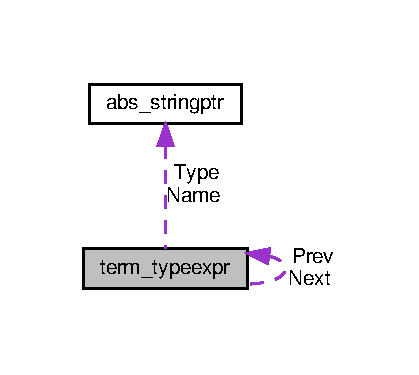
\includegraphics[width=202pt]{db/de8/structterm__typeexpr__coll__graph}
\end{center}
\end{figure}
\doxysubsection*{Public Attributes}
\begin{DoxyCompactItemize}
\item 
st\+\_\+ptr \mbox{\hyperlink{structterm__typeexpr_aa33dcc1345202efe5929d00019e226e5}{Type}}
\item 
st\+\_\+ptr \mbox{\hyperlink{structterm__typeexpr_a2510ec68bc76b3b2aa7a6391018750bc}{Name}}
\item 
b8 \mbox{\hyperlink{structterm__typeexpr_a93ac336807d6f45f5bd6270f21b02679}{is\+Ptr}}
\item 
b8 \mbox{\hyperlink{structterm__typeexpr_aa8779ec62ac26dd1239060953fd65f56}{is\+Reference}}
\item 
b8 \mbox{\hyperlink{structterm__typeexpr_af67982c68088bdca49bdcd1738bb7b7a}{is\+Const}}
\item 
b8 \mbox{\hyperlink{structterm__typeexpr_a2bc07d643069855d995bbcd4fa81006c}{is\+Array}}
\item 
s32 \mbox{\hyperlink{structterm__typeexpr_ab93773f58c02499d82f1dd1188182506}{Array\+Length}}
\item 
\mbox{\hyperlink{ab__parser_8h_ac9039717ce4cccacf493ee306650a423}{custom\+\_\+type}} \mbox{\hyperlink{structterm__typeexpr_a9544ece5f851486a3a725c0bd87df73f}{Custom\+Type}}
\item 
\mbox{\hyperlink{structterm__typeexpr}{term\+\_\+typeexpr}} $\ast$ \mbox{\hyperlink{structterm__typeexpr_a827f986754feb8a31cb88bb5929f35cb}{Next}}
\item 
\mbox{\hyperlink{structterm__typeexpr}{term\+\_\+typeexpr}} $\ast$ \mbox{\hyperlink{structterm__typeexpr_ac489d3375eb8507325fd21d328bdf2cc}{Prev}}
\end{DoxyCompactItemize}


\doxysubsection{Member Data Documentation}
\mbox{\Hypertarget{structterm__typeexpr_ab93773f58c02499d82f1dd1188182506}\label{structterm__typeexpr_ab93773f58c02499d82f1dd1188182506}} 
\index{term\_typeexpr@{term\_typeexpr}!ArrayLength@{ArrayLength}}
\index{ArrayLength@{ArrayLength}!term\_typeexpr@{term\_typeexpr}}
\doxysubsubsection{\texorpdfstring{ArrayLength}{ArrayLength}}
{\footnotesize\ttfamily s32 term\+\_\+typeexpr\+::\+Array\+Length}

\mbox{\Hypertarget{structterm__typeexpr_a9544ece5f851486a3a725c0bd87df73f}\label{structterm__typeexpr_a9544ece5f851486a3a725c0bd87df73f}} 
\index{term\_typeexpr@{term\_typeexpr}!CustomType@{CustomType}}
\index{CustomType@{CustomType}!term\_typeexpr@{term\_typeexpr}}
\doxysubsubsection{\texorpdfstring{CustomType}{CustomType}}
{\footnotesize\ttfamily \mbox{\hyperlink{ab__parser_8h_ac9039717ce4cccacf493ee306650a423}{custom\+\_\+type}} term\+\_\+typeexpr\+::\+Custom\+Type}

\mbox{\Hypertarget{structterm__typeexpr_a2bc07d643069855d995bbcd4fa81006c}\label{structterm__typeexpr_a2bc07d643069855d995bbcd4fa81006c}} 
\index{term\_typeexpr@{term\_typeexpr}!isArray@{isArray}}
\index{isArray@{isArray}!term\_typeexpr@{term\_typeexpr}}
\doxysubsubsection{\texorpdfstring{isArray}{isArray}}
{\footnotesize\ttfamily b8 term\+\_\+typeexpr\+::is\+Array}

\mbox{\Hypertarget{structterm__typeexpr_af67982c68088bdca49bdcd1738bb7b7a}\label{structterm__typeexpr_af67982c68088bdca49bdcd1738bb7b7a}} 
\index{term\_typeexpr@{term\_typeexpr}!isConst@{isConst}}
\index{isConst@{isConst}!term\_typeexpr@{term\_typeexpr}}
\doxysubsubsection{\texorpdfstring{isConst}{isConst}}
{\footnotesize\ttfamily b8 term\+\_\+typeexpr\+::is\+Const}

\mbox{\Hypertarget{structterm__typeexpr_a93ac336807d6f45f5bd6270f21b02679}\label{structterm__typeexpr_a93ac336807d6f45f5bd6270f21b02679}} 
\index{term\_typeexpr@{term\_typeexpr}!isPtr@{isPtr}}
\index{isPtr@{isPtr}!term\_typeexpr@{term\_typeexpr}}
\doxysubsubsection{\texorpdfstring{isPtr}{isPtr}}
{\footnotesize\ttfamily b8 term\+\_\+typeexpr\+::is\+Ptr}

\mbox{\Hypertarget{structterm__typeexpr_aa8779ec62ac26dd1239060953fd65f56}\label{structterm__typeexpr_aa8779ec62ac26dd1239060953fd65f56}} 
\index{term\_typeexpr@{term\_typeexpr}!isReference@{isReference}}
\index{isReference@{isReference}!term\_typeexpr@{term\_typeexpr}}
\doxysubsubsection{\texorpdfstring{isReference}{isReference}}
{\footnotesize\ttfamily b8 term\+\_\+typeexpr\+::is\+Reference}

\mbox{\Hypertarget{structterm__typeexpr_a2510ec68bc76b3b2aa7a6391018750bc}\label{structterm__typeexpr_a2510ec68bc76b3b2aa7a6391018750bc}} 
\index{term\_typeexpr@{term\_typeexpr}!Name@{Name}}
\index{Name@{Name}!term\_typeexpr@{term\_typeexpr}}
\doxysubsubsection{\texorpdfstring{Name}{Name}}
{\footnotesize\ttfamily st\+\_\+ptr term\+\_\+typeexpr\+::\+Name}

\mbox{\Hypertarget{structterm__typeexpr_a827f986754feb8a31cb88bb5929f35cb}\label{structterm__typeexpr_a827f986754feb8a31cb88bb5929f35cb}} 
\index{term\_typeexpr@{term\_typeexpr}!Next@{Next}}
\index{Next@{Next}!term\_typeexpr@{term\_typeexpr}}
\doxysubsubsection{\texorpdfstring{Next}{Next}}
{\footnotesize\ttfamily \mbox{\hyperlink{structterm__typeexpr}{term\+\_\+typeexpr}}$\ast$ term\+\_\+typeexpr\+::\+Next}

\mbox{\Hypertarget{structterm__typeexpr_ac489d3375eb8507325fd21d328bdf2cc}\label{structterm__typeexpr_ac489d3375eb8507325fd21d328bdf2cc}} 
\index{term\_typeexpr@{term\_typeexpr}!Prev@{Prev}}
\index{Prev@{Prev}!term\_typeexpr@{term\_typeexpr}}
\doxysubsubsection{\texorpdfstring{Prev}{Prev}}
{\footnotesize\ttfamily \mbox{\hyperlink{structterm__typeexpr}{term\+\_\+typeexpr}}$\ast$ term\+\_\+typeexpr\+::\+Prev}

\mbox{\Hypertarget{structterm__typeexpr_aa33dcc1345202efe5929d00019e226e5}\label{structterm__typeexpr_aa33dcc1345202efe5929d00019e226e5}} 
\index{term\_typeexpr@{term\_typeexpr}!Type@{Type}}
\index{Type@{Type}!term\_typeexpr@{term\_typeexpr}}
\doxysubsubsection{\texorpdfstring{Type}{Type}}
{\footnotesize\ttfamily st\+\_\+ptr term\+\_\+typeexpr\+::\+Type}



The documentation for this struct was generated from the following file\+:\begin{DoxyCompactItemize}
\item 
\mbox{\hyperlink{ab__parser_8h}{ab\+\_\+parser.\+h}}\end{DoxyCompactItemize}

\hypertarget{structtest__cmd__queue}{}\section{test\+\_\+cmd\+\_\+queue Struct Reference}
\label{structtest__cmd__queue}\index{test\+\_\+cmd\+\_\+queue@{test\+\_\+cmd\+\_\+queue}}


A circular queue of 10 elements for the state command test\+\_\+cmd.  




{\ttfamily \#include $<$Generated\+\_\+\+Test.\+h$>$}

\subsection*{Public Attributes}
\begin{DoxyCompactItemize}
\item 
\hyperlink{PreprocTest_8h_a55ed691059222a58555cf9992ec14431}{test\+\_\+cmd} \hyperlink{structtest__cmd__queue_a893fe182353a750337200b5aad9bacb3}{Items} \mbox{[}10\mbox{]}
\item 
s32 \hyperlink{structtest__cmd__queue_a20ed55b6b8b836106c001539d2e3d599}{Front}
\item 
s32 \hyperlink{structtest__cmd__queue_a7cedef36f33507cbadf3f4ef95aa7cec}{Rear}
\end{DoxyCompactItemize}


\subsection{Detailed Description}
A circular queue of 10 elements for the state command test\+\_\+cmd. 

\subsection{Member Data Documentation}
\mbox{\Hypertarget{structtest__cmd__queue_a20ed55b6b8b836106c001539d2e3d599}\label{structtest__cmd__queue_a20ed55b6b8b836106c001539d2e3d599}} 
\index{test\+\_\+cmd\+\_\+queue@{test\+\_\+cmd\+\_\+queue}!Front@{Front}}
\index{Front@{Front}!test\+\_\+cmd\+\_\+queue@{test\+\_\+cmd\+\_\+queue}}
\subsubsection{\texorpdfstring{Front}{Front}}
{\footnotesize\ttfamily s32 test\+\_\+cmd\+\_\+queue\+::\+Front}

\mbox{\Hypertarget{structtest__cmd__queue_a893fe182353a750337200b5aad9bacb3}\label{structtest__cmd__queue_a893fe182353a750337200b5aad9bacb3}} 
\index{test\+\_\+cmd\+\_\+queue@{test\+\_\+cmd\+\_\+queue}!Items@{Items}}
\index{Items@{Items}!test\+\_\+cmd\+\_\+queue@{test\+\_\+cmd\+\_\+queue}}
\subsubsection{\texorpdfstring{Items}{Items}}
{\footnotesize\ttfamily \hyperlink{PreprocTest_8h_a55ed691059222a58555cf9992ec14431}{test\+\_\+cmd} test\+\_\+cmd\+\_\+queue\+::\+Items\mbox{[}10\mbox{]}}

\mbox{\Hypertarget{structtest__cmd__queue_a7cedef36f33507cbadf3f4ef95aa7cec}\label{structtest__cmd__queue_a7cedef36f33507cbadf3f4ef95aa7cec}} 
\index{test\+\_\+cmd\+\_\+queue@{test\+\_\+cmd\+\_\+queue}!Rear@{Rear}}
\index{Rear@{Rear}!test\+\_\+cmd\+\_\+queue@{test\+\_\+cmd\+\_\+queue}}
\subsubsection{\texorpdfstring{Rear}{Rear}}
{\footnotesize\ttfamily s32 test\+\_\+cmd\+\_\+queue\+::\+Rear}



The documentation for this struct was generated from the following file\+:\begin{DoxyCompactItemize}
\item 
\hyperlink{Generated__Test_8h}{Generated\+\_\+\+Test.\+h}\end{DoxyCompactItemize}

\hypertarget{structtest__suite__token__list__item}{}\section{test\+\_\+suite\+\_\+token\+\_\+list\+\_\+item Struct Reference}
\label{structtest__suite__token__list__item}\index{test\+\_\+suite\+\_\+token\+\_\+list\+\_\+item@{test\+\_\+suite\+\_\+token\+\_\+list\+\_\+item}}


Collaboration diagram for test\+\_\+suite\+\_\+token\+\_\+list\+\_\+item\+:
\nopagebreak
\begin{figure}[H]
\begin{center}
\leavevmode
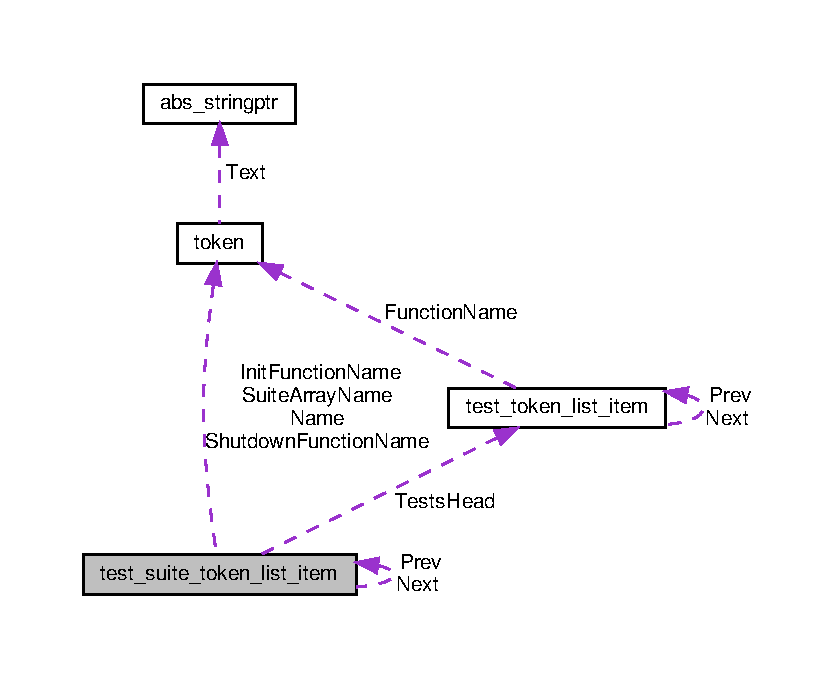
\includegraphics[width=350pt]{da/d06/structtest__suite__token__list__item__coll__graph}
\end{center}
\end{figure}
\subsection*{Public Attributes}
\begin{DoxyCompactItemize}
\item 
\hyperlink{structtoken}{token} \hyperlink{structtest__suite__token__list__item_a63834f736499a8eb9a5be4ce658ad420}{Name}
\item 
\hyperlink{structtoken}{token} \hyperlink{structtest__suite__token__list__item_a33bab1f9cd9b0c869eadfcbde0320d86}{Suite\+Array\+Name}
\item 
\hyperlink{structtoken}{token} \hyperlink{structtest__suite__token__list__item_a3d7b2baf23150725e91f919067ec6d81}{Init\+Function\+Name}
\item 
\hyperlink{structtoken}{token} \hyperlink{structtest__suite__token__list__item_a0577805f0d8627a70a98882765c9a2b9}{Shutdown\+Function\+Name}
\item 
\hyperlink{structtest__token__list__item}{test\+\_\+token\+\_\+list\+\_\+item} \hyperlink{structtest__suite__token__list__item_a733adf7402d148f6d1d713f7ad08b835}{Tests\+Head}
\item 
\hyperlink{structtest__suite__token__list__item}{test\+\_\+suite\+\_\+token\+\_\+list\+\_\+item} $\ast$ \hyperlink{structtest__suite__token__list__item_aa9d98f0ebaaa60117452f83b01a5f875}{Next}
\item 
\hyperlink{structtest__suite__token__list__item}{test\+\_\+suite\+\_\+token\+\_\+list\+\_\+item} $\ast$ \hyperlink{structtest__suite__token__list__item_a0bbc26a13de896100669c60385883fd2}{Prev}
\end{DoxyCompactItemize}


\subsection{Member Data Documentation}
\mbox{\Hypertarget{structtest__suite__token__list__item_a3d7b2baf23150725e91f919067ec6d81}\label{structtest__suite__token__list__item_a3d7b2baf23150725e91f919067ec6d81}} 
\index{test\+\_\+suite\+\_\+token\+\_\+list\+\_\+item@{test\+\_\+suite\+\_\+token\+\_\+list\+\_\+item}!Init\+Function\+Name@{Init\+Function\+Name}}
\index{Init\+Function\+Name@{Init\+Function\+Name}!test\+\_\+suite\+\_\+token\+\_\+list\+\_\+item@{test\+\_\+suite\+\_\+token\+\_\+list\+\_\+item}}
\subsubsection{\texorpdfstring{Init\+Function\+Name}{InitFunctionName}}
{\footnotesize\ttfamily \hyperlink{structtoken}{token} test\+\_\+suite\+\_\+token\+\_\+list\+\_\+item\+::\+Init\+Function\+Name}

\mbox{\Hypertarget{structtest__suite__token__list__item_a63834f736499a8eb9a5be4ce658ad420}\label{structtest__suite__token__list__item_a63834f736499a8eb9a5be4ce658ad420}} 
\index{test\+\_\+suite\+\_\+token\+\_\+list\+\_\+item@{test\+\_\+suite\+\_\+token\+\_\+list\+\_\+item}!Name@{Name}}
\index{Name@{Name}!test\+\_\+suite\+\_\+token\+\_\+list\+\_\+item@{test\+\_\+suite\+\_\+token\+\_\+list\+\_\+item}}
\subsubsection{\texorpdfstring{Name}{Name}}
{\footnotesize\ttfamily \hyperlink{structtoken}{token} test\+\_\+suite\+\_\+token\+\_\+list\+\_\+item\+::\+Name}

\mbox{\Hypertarget{structtest__suite__token__list__item_aa9d98f0ebaaa60117452f83b01a5f875}\label{structtest__suite__token__list__item_aa9d98f0ebaaa60117452f83b01a5f875}} 
\index{test\+\_\+suite\+\_\+token\+\_\+list\+\_\+item@{test\+\_\+suite\+\_\+token\+\_\+list\+\_\+item}!Next@{Next}}
\index{Next@{Next}!test\+\_\+suite\+\_\+token\+\_\+list\+\_\+item@{test\+\_\+suite\+\_\+token\+\_\+list\+\_\+item}}
\subsubsection{\texorpdfstring{Next}{Next}}
{\footnotesize\ttfamily \hyperlink{structtest__suite__token__list__item}{test\+\_\+suite\+\_\+token\+\_\+list\+\_\+item}$\ast$ test\+\_\+suite\+\_\+token\+\_\+list\+\_\+item\+::\+Next}

\mbox{\Hypertarget{structtest__suite__token__list__item_a0bbc26a13de896100669c60385883fd2}\label{structtest__suite__token__list__item_a0bbc26a13de896100669c60385883fd2}} 
\index{test\+\_\+suite\+\_\+token\+\_\+list\+\_\+item@{test\+\_\+suite\+\_\+token\+\_\+list\+\_\+item}!Prev@{Prev}}
\index{Prev@{Prev}!test\+\_\+suite\+\_\+token\+\_\+list\+\_\+item@{test\+\_\+suite\+\_\+token\+\_\+list\+\_\+item}}
\subsubsection{\texorpdfstring{Prev}{Prev}}
{\footnotesize\ttfamily \hyperlink{structtest__suite__token__list__item}{test\+\_\+suite\+\_\+token\+\_\+list\+\_\+item}$\ast$ test\+\_\+suite\+\_\+token\+\_\+list\+\_\+item\+::\+Prev}

\mbox{\Hypertarget{structtest__suite__token__list__item_a0577805f0d8627a70a98882765c9a2b9}\label{structtest__suite__token__list__item_a0577805f0d8627a70a98882765c9a2b9}} 
\index{test\+\_\+suite\+\_\+token\+\_\+list\+\_\+item@{test\+\_\+suite\+\_\+token\+\_\+list\+\_\+item}!Shutdown\+Function\+Name@{Shutdown\+Function\+Name}}
\index{Shutdown\+Function\+Name@{Shutdown\+Function\+Name}!test\+\_\+suite\+\_\+token\+\_\+list\+\_\+item@{test\+\_\+suite\+\_\+token\+\_\+list\+\_\+item}}
\subsubsection{\texorpdfstring{Shutdown\+Function\+Name}{ShutdownFunctionName}}
{\footnotesize\ttfamily \hyperlink{structtoken}{token} test\+\_\+suite\+\_\+token\+\_\+list\+\_\+item\+::\+Shutdown\+Function\+Name}

\mbox{\Hypertarget{structtest__suite__token__list__item_a33bab1f9cd9b0c869eadfcbde0320d86}\label{structtest__suite__token__list__item_a33bab1f9cd9b0c869eadfcbde0320d86}} 
\index{test\+\_\+suite\+\_\+token\+\_\+list\+\_\+item@{test\+\_\+suite\+\_\+token\+\_\+list\+\_\+item}!Suite\+Array\+Name@{Suite\+Array\+Name}}
\index{Suite\+Array\+Name@{Suite\+Array\+Name}!test\+\_\+suite\+\_\+token\+\_\+list\+\_\+item@{test\+\_\+suite\+\_\+token\+\_\+list\+\_\+item}}
\subsubsection{\texorpdfstring{Suite\+Array\+Name}{SuiteArrayName}}
{\footnotesize\ttfamily \hyperlink{structtoken}{token} test\+\_\+suite\+\_\+token\+\_\+list\+\_\+item\+::\+Suite\+Array\+Name}

\mbox{\Hypertarget{structtest__suite__token__list__item_a733adf7402d148f6d1d713f7ad08b835}\label{structtest__suite__token__list__item_a733adf7402d148f6d1d713f7ad08b835}} 
\index{test\+\_\+suite\+\_\+token\+\_\+list\+\_\+item@{test\+\_\+suite\+\_\+token\+\_\+list\+\_\+item}!Tests\+Head@{Tests\+Head}}
\index{Tests\+Head@{Tests\+Head}!test\+\_\+suite\+\_\+token\+\_\+list\+\_\+item@{test\+\_\+suite\+\_\+token\+\_\+list\+\_\+item}}
\subsubsection{\texorpdfstring{Tests\+Head}{TestsHead}}
{\footnotesize\ttfamily \hyperlink{structtest__token__list__item}{test\+\_\+token\+\_\+list\+\_\+item} test\+\_\+suite\+\_\+token\+\_\+list\+\_\+item\+::\+Tests\+Head}



The documentation for this struct was generated from the following file\+:\begin{DoxyCompactItemize}
\item 
\hyperlink{test__preprocessor_8cpp}{test\+\_\+preprocessor.\+cpp}\end{DoxyCompactItemize}

\hypertarget{structtest__token__list__item}{}\section{test\+\_\+token\+\_\+list\+\_\+item Struct Reference}
\label{structtest__token__list__item}\index{test\+\_\+token\+\_\+list\+\_\+item@{test\+\_\+token\+\_\+list\+\_\+item}}


Collaboration diagram for test\+\_\+token\+\_\+list\+\_\+item\+:\nopagebreak
\begin{figure}[H]
\begin{center}
\leavevmode
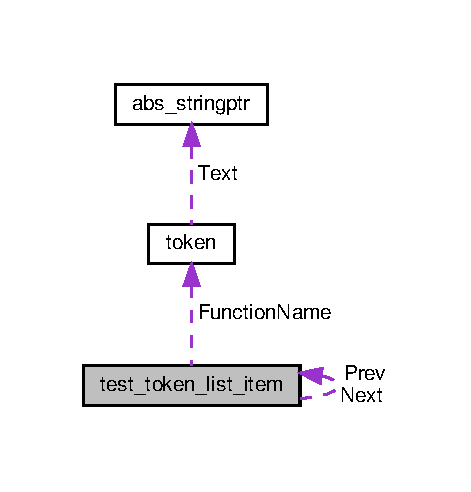
\includegraphics[width=226pt]{d0/d11/structtest__token__list__item__coll__graph}
\end{center}
\end{figure}
\subsection*{Public Attributes}
\begin{DoxyCompactItemize}
\item 
\hyperlink{structtoken}{token} \hyperlink{structtest__token__list__item_a48319a908d351d150a224fd1ece758d7}{Function\+Name}
\item 
token\+\_\+list\+\_\+item \hyperlink{structtest__token__list__item_a30e55573c651ec80614b75f9b180dc80}{Test\+Steps\+Head}
\item 
\hyperlink{structtest__token__list__item}{test\+\_\+token\+\_\+list\+\_\+item} $\ast$ \hyperlink{structtest__token__list__item_a271ea32ddd03b4f6bb44237881915692}{Next}
\item 
\hyperlink{structtest__token__list__item}{test\+\_\+token\+\_\+list\+\_\+item} $\ast$ \hyperlink{structtest__token__list__item_aa053b5098e750d72759f6520d287c74d}{Prev}
\end{DoxyCompactItemize}


\subsection{Member Data Documentation}
\mbox{\Hypertarget{structtest__token__list__item_a48319a908d351d150a224fd1ece758d7}\label{structtest__token__list__item_a48319a908d351d150a224fd1ece758d7}} 
\index{test\+\_\+token\+\_\+list\+\_\+item@{test\+\_\+token\+\_\+list\+\_\+item}!Function\+Name@{Function\+Name}}
\index{Function\+Name@{Function\+Name}!test\+\_\+token\+\_\+list\+\_\+item@{test\+\_\+token\+\_\+list\+\_\+item}}
\subsubsection{\texorpdfstring{Function\+Name}{FunctionName}}
{\footnotesize\ttfamily \hyperlink{structtoken}{token} test\+\_\+token\+\_\+list\+\_\+item\+::\+Function\+Name}

\mbox{\Hypertarget{structtest__token__list__item_a271ea32ddd03b4f6bb44237881915692}\label{structtest__token__list__item_a271ea32ddd03b4f6bb44237881915692}} 
\index{test\+\_\+token\+\_\+list\+\_\+item@{test\+\_\+token\+\_\+list\+\_\+item}!Next@{Next}}
\index{Next@{Next}!test\+\_\+token\+\_\+list\+\_\+item@{test\+\_\+token\+\_\+list\+\_\+item}}
\subsubsection{\texorpdfstring{Next}{Next}}
{\footnotesize\ttfamily \hyperlink{structtest__token__list__item}{test\+\_\+token\+\_\+list\+\_\+item}$\ast$ test\+\_\+token\+\_\+list\+\_\+item\+::\+Next}

\mbox{\Hypertarget{structtest__token__list__item_aa053b5098e750d72759f6520d287c74d}\label{structtest__token__list__item_aa053b5098e750d72759f6520d287c74d}} 
\index{test\+\_\+token\+\_\+list\+\_\+item@{test\+\_\+token\+\_\+list\+\_\+item}!Prev@{Prev}}
\index{Prev@{Prev}!test\+\_\+token\+\_\+list\+\_\+item@{test\+\_\+token\+\_\+list\+\_\+item}}
\subsubsection{\texorpdfstring{Prev}{Prev}}
{\footnotesize\ttfamily \hyperlink{structtest__token__list__item}{test\+\_\+token\+\_\+list\+\_\+item}$\ast$ test\+\_\+token\+\_\+list\+\_\+item\+::\+Prev}

\mbox{\Hypertarget{structtest__token__list__item_a30e55573c651ec80614b75f9b180dc80}\label{structtest__token__list__item_a30e55573c651ec80614b75f9b180dc80}} 
\index{test\+\_\+token\+\_\+list\+\_\+item@{test\+\_\+token\+\_\+list\+\_\+item}!Test\+Steps\+Head@{Test\+Steps\+Head}}
\index{Test\+Steps\+Head@{Test\+Steps\+Head}!test\+\_\+token\+\_\+list\+\_\+item@{test\+\_\+token\+\_\+list\+\_\+item}}
\subsubsection{\texorpdfstring{Test\+Steps\+Head}{TestStepsHead}}
{\footnotesize\ttfamily token\+\_\+list\+\_\+item test\+\_\+token\+\_\+list\+\_\+item\+::\+Test\+Steps\+Head}



The documentation for this struct was generated from the following file\+:\begin{DoxyCompactItemize}
\item 
\hyperlink{test__preprocessor_8cpp}{test\+\_\+preprocessor.\+cpp}\end{DoxyCompactItemize}

\hypertarget{structtest__type}{}\doxysection{test\+\_\+type Struct Reference}
\label{structtest__type}\index{test\_type@{test\_type}}


{\ttfamily \#include $<$Preproc\+Test.\+h$>$}



Collaboration diagram for test\+\_\+type\+:\nopagebreak
\begin{figure}[H]
\begin{center}
\leavevmode
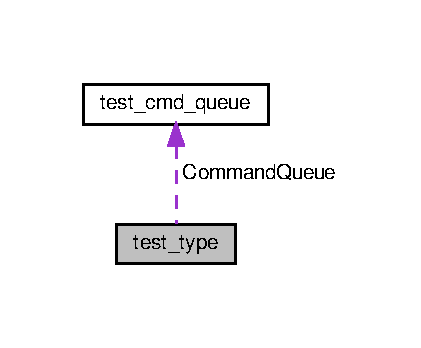
\includegraphics[width=202pt]{d5/dfe/structtest__type__coll__graph}
\end{center}
\end{figure}
\doxysubsection*{Public Attributes}
\begin{DoxyCompactItemize}
\item 
test\+\_\+statemachine $\ast$ \mbox{\hyperlink{structtest__type_a48139457e16e23a57531e5af02be7f14}{Current\+State}}
\item 
b8 \mbox{\hyperlink{structtest__type_a36eb3041ef1341aec27a2a2d98500ce6}{is\+New\+State}}
\item 
\mbox{\hyperlink{structtest__cmd__queue}{test\+\_\+cmd\+\_\+queue}} \mbox{\hyperlink{structtest__type_a9ef32b05c6f8a712062f8261d71665ca}{Command\+Queue}}
\end{DoxyCompactItemize}


\doxysubsection{Member Data Documentation}
\mbox{\Hypertarget{structtest__type_a9ef32b05c6f8a712062f8261d71665ca}\label{structtest__type_a9ef32b05c6f8a712062f8261d71665ca}} 
\index{test\_type@{test\_type}!CommandQueue@{CommandQueue}}
\index{CommandQueue@{CommandQueue}!test\_type@{test\_type}}
\doxysubsubsection{\texorpdfstring{CommandQueue}{CommandQueue}}
{\footnotesize\ttfamily \mbox{\hyperlink{structtest__cmd__queue}{test\+\_\+cmd\+\_\+queue}} test\+\_\+type\+::\+Command\+Queue}

\mbox{\Hypertarget{structtest__type_a48139457e16e23a57531e5af02be7f14}\label{structtest__type_a48139457e16e23a57531e5af02be7f14}} 
\index{test\_type@{test\_type}!CurrentState@{CurrentState}}
\index{CurrentState@{CurrentState}!test\_type@{test\_type}}
\doxysubsubsection{\texorpdfstring{CurrentState}{CurrentState}}
{\footnotesize\ttfamily test\+\_\+statemachine$\ast$ test\+\_\+type\+::\+Current\+State}

\mbox{\Hypertarget{structtest__type_a36eb3041ef1341aec27a2a2d98500ce6}\label{structtest__type_a36eb3041ef1341aec27a2a2d98500ce6}} 
\index{test\_type@{test\_type}!isNewState@{isNewState}}
\index{isNewState@{isNewState}!test\_type@{test\_type}}
\doxysubsubsection{\texorpdfstring{isNewState}{isNewState}}
{\footnotesize\ttfamily b8 test\+\_\+type\+::is\+New\+State}



The documentation for this struct was generated from the following file\+:\begin{DoxyCompactItemize}
\item 
\mbox{\hyperlink{PreprocTest_8h}{Preproc\+Test.\+h}}\end{DoxyCompactItemize}

\hypertarget{structtoken}{}\doxysection{token Struct Reference}
\label{structtoken}\index{token@{token}}


{\ttfamily \#include $<$ab\+\_\+lexer.\+h$>$}

\doxysubsection*{Public Attributes}
\begin{DoxyCompactItemize}
\item 
\mbox{\hyperlink{ab__lexer_8h_afe5ef662303b6b710ea6ee1a944bad0d}{token\+\_\+type}} \mbox{\hyperlink{structtoken_a82914c351900753f626fa2d6fcb12fde}{Type}}
\item 
abs\+\_\+stringptr \mbox{\hyperlink{structtoken_afe96285022144ed40a345ac60d688550}{Text}}
\end{DoxyCompactItemize}


\doxysubsection{Member Data Documentation}
\mbox{\Hypertarget{structtoken_afe96285022144ed40a345ac60d688550}\label{structtoken_afe96285022144ed40a345ac60d688550}} 
\index{token@{token}!Text@{Text}}
\index{Text@{Text}!token@{token}}
\doxysubsubsection{\texorpdfstring{Text}{Text}}
{\footnotesize\ttfamily abs\+\_\+stringptr token\+::\+Text}

\mbox{\Hypertarget{structtoken_a82914c351900753f626fa2d6fcb12fde}\label{structtoken_a82914c351900753f626fa2d6fcb12fde}} 
\index{token@{token}!Type@{Type}}
\index{Type@{Type}!token@{token}}
\doxysubsubsection{\texorpdfstring{Type}{Type}}
{\footnotesize\ttfamily \mbox{\hyperlink{ab__lexer_8h_afe5ef662303b6b710ea6ee1a944bad0d}{token\+\_\+type}} token\+::\+Type}



The documentation for this struct was generated from the following file\+:\begin{DoxyCompactItemize}
\item 
\mbox{\hyperlink{ab__lexer_8h}{ab\+\_\+lexer.\+h}}\end{DoxyCompactItemize}

\chapter{File Documentation}
\hypertarget{ab__common_8h}{}\doxysection{ab\+\_\+common.\+h File Reference}
\label{ab__common_8h}\index{ab\_common.h@{ab\_common.h}}


Common macros and typedefs.  


{\ttfamily \#include $<$stdint.\+h$>$}\newline
{\ttfamily \#include $<$wchar.\+h$>$}\newline
Include dependency graph for ab\+\_\+common.\+h\+:\nopagebreak
\begin{figure}[H]
\begin{center}
\leavevmode
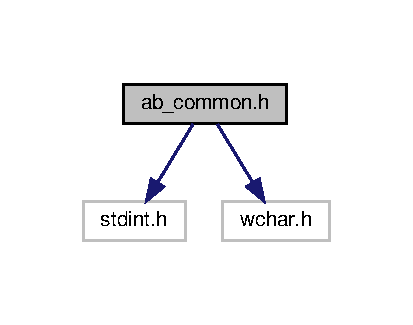
\includegraphics[width=198pt]{d1/dd0/ab__common_8h__incl}
\end{center}
\end{figure}
This graph shows which files directly or indirectly include this file\+:\nopagebreak
\begin{figure}[H]
\begin{center}
\leavevmode
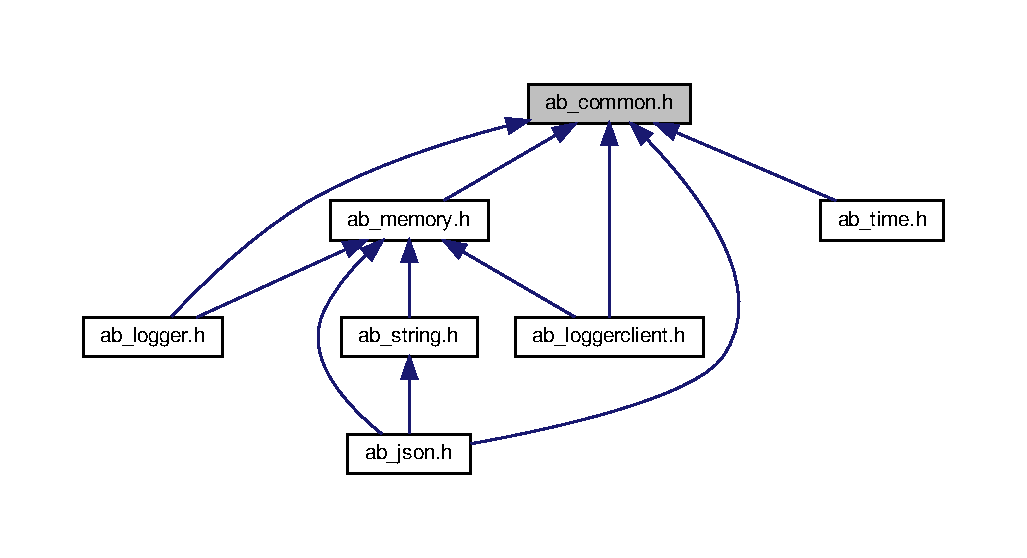
\includegraphics[width=335pt]{d8/da5/ab__common_8h__dep__incl}
\end{center}
\end{figure}
\doxysubsection*{Macros}
\begin{DoxyCompactItemize}
\item 
\#define \mbox{\hyperlink{ab__common_8h_a49450bdfb96baf39e5679e3749dd6648}{Array\+Count}}(Array)~(sizeof(Array)) / (sizeof(Array\mbox{[}0\mbox{]}))
\begin{DoxyCompactList}\small\item\em Macro that can be used anywhere with a pre-\/defined array. \end{DoxyCompactList}\item 
\#define \mbox{\hyperlink{ab__common_8h_a1da41d527b391b557b30acdc9e2cf425}{M\+A\+X\+\_\+\+F\+I\+L\+E\+N\+A\+M\+E\+\_\+\+S\+I\+ZE}}~255
\item 
\#define \mbox{\hyperlink{ab__common_8h_ab569440ccd9ea3398cfc4d514fb5493f}{M\+I\+N\+I\+M\+UM}}(Value1,  Value2)~(((Value1) $<$ (Value2)) ? (Value1) \+: (Value2))
\begin{DoxyCompactList}\small\item\em Return the minimum of a value. \end{DoxyCompactList}\item 
\#define \mbox{\hyperlink{ab__common_8h_aa0dcb9de6453c0e93a7d4c26739380e2}{M\+A\+X\+I\+M\+UM}}(Value1,  Value2)~(((Value1) $>$ (Value2)) ? (Value1) \+: (Value2))
\begin{DoxyCompactList}\small\item\em Return the maximum of a value. \end{DoxyCompactList}\item 
\#define \mbox{\hyperlink{ab__common_8h_a20bc847a34a521a2e6fa125621be9bfc}{Bit\+Reset}}(Value,  Bit)~((Value) \&= $\sim$(1 $<$$<$ (Bit)))
\begin{DoxyCompactList}\small\item\em Reset the bit to zero. \end{DoxyCompactList}\item 
\#define \mbox{\hyperlink{ab__common_8h_a1eeb0506b4ddd8d37c817456de87f052}{Bit\+Set}}(Value,  Bit)~((Value) $\vert$= (1 $<$$<$ (Bit)))
\begin{DoxyCompactList}\small\item\em Set the bit to one. \end{DoxyCompactList}\item 
\#define \mbox{\hyperlink{ab__common_8h_a9e89c74d1fedd0a954107d7ab01481cc}{Kilobytes}}(num)~(1024U\+LL $\ast$ (num))
\item 
\#define \mbox{\hyperlink{ab__common_8h_a2617ed135c31ace7205aae9398392eca}{Megabytes}}(num)~(1024U\+LL $\ast$ \mbox{\hyperlink{ab__common_8h_a9e89c74d1fedd0a954107d7ab01481cc}{Kilobytes}}(num))
\item 
\#define \mbox{\hyperlink{ab__common_8h_ae0b63ae9651c6178680d84f4900e0a0d}{Gigabytes}}(num)~(1024U\+LL $\ast$ \mbox{\hyperlink{ab__common_8h_a2617ed135c31ace7205aae9398392eca}{Megabytes}}(num))
\item 
\#define \mbox{\hyperlink{ab__common_8h_aa01ae46693c8d6cada0f39d78e8da9f8}{Terabytes}}(num)~(1024U\+LL $\ast$ \mbox{\hyperlink{ab__common_8h_ae0b63ae9651c6178680d84f4900e0a0d}{Gigabytes}}(num))
\item 
\#define \mbox{\hyperlink{ab__common_8h_a20fa811b86f3ecd1f72ae57753c26d56}{S\+\_\+\+T\+O\+\_\+\+MS}}(num)~((num) $\ast$ 1000L)
\item 
\#define \mbox{\hyperlink{ab__common_8h_ad8619bfe2bde192cdb90aaa749de313a}{S\+\_\+\+T\+O\+\_\+\+NS}}(num)~((num) $\ast$ 1e9L)
\item 
\#define \mbox{\hyperlink{ab__common_8h_af99d895a4fb9ef16b8773bfb4682cb0b}{M\+S\+\_\+\+T\+O\+\_\+S}}(num)~((num) $\ast$ 0.\+001f)
\item 
\#define \mbox{\hyperlink{ab__common_8h_a830e4dd55a9d1f281527e77f61993194}{M\+S\+\_\+\+T\+O\+\_\+\+NS}}(num)~((num) $\ast$ 1000000.\+0f)
\item 
\#define \mbox{\hyperlink{ab__common_8h_a5ea52ba9d4cb9e553e52d1c7283b58a7}{N\+S\+\_\+\+T\+O\+\_\+S}}(num)~((num) $\ast$ 1e-\/9f)
\item 
\#define \mbox{\hyperlink{ab__common_8h_a323127aaf9260b4e2092a8734886379a}{N\+S\+\_\+\+T\+O\+\_\+\+MS}}(num)~((num) $\ast$ 1e-\/6f)
\item 
\#define \mbox{\hyperlink{ab__common_8h_af2b46bb19c7d3d91950a9f971d443ccd}{Assert}}(test)
\begin{DoxyCompactList}\small\item\em Assert causes a hard-\/fault, useful when debugging. Don\textquotesingle{}t use this is production code. \end{DoxyCompactList}\end{DoxyCompactItemize}
\doxysubsection*{Typedefs}
\begin{DoxyCompactItemize}
\item 
typedef wchar\+\_\+t \mbox{\hyperlink{ab__common_8h_a59dcfa356b98a549d778585b6b0388e3}{wchar}}
\item 
typedef int8\+\_\+t \mbox{\hyperlink{ab__common_8h_a70e369648385b50f2d0588e8e8745275}{b8}}
\item 
typedef int8\+\_\+t \mbox{\hyperlink{ab__common_8h_a9e382f207c65ca13ab4ae98363aeda80}{s8}}
\item 
typedef uint8\+\_\+t \mbox{\hyperlink{ab__common_8h_a92c50087ca0e64fa93fc59402c55f8ca}{u8}}
\item 
typedef int16\+\_\+t \mbox{\hyperlink{ab__common_8h_aa980e2c02ba2305e0f489d5650655425}{s16}}
\item 
typedef uint16\+\_\+t \mbox{\hyperlink{ab__common_8h_ace9d960e74685e2cd84b36132dbbf8aa}{u16}}
\item 
typedef int32\+\_\+t \mbox{\hyperlink{ab__common_8h_ae9b1af5c037e57a98884758875d3a7c4}{s32}}
\item 
typedef uint32\+\_\+t \mbox{\hyperlink{ab__common_8h_afaa62991928fb9fb18ff0db62a040aba}{u32}}
\item 
typedef int64\+\_\+t \mbox{\hyperlink{ab__common_8h_a350c6fc928e3bdc6c6486268ac8fb269}{s64}}
\item 
typedef uint64\+\_\+t \mbox{\hyperlink{ab__common_8h_a3f7e2bcbb0b4c338f3c4f6c937cd4234}{u64}}
\item 
typedef float \mbox{\hyperlink{ab__common_8h_aafa04bc3cb166e826b75a23f4add4b59}{r32}}
\item 
typedef double \mbox{\hyperlink{ab__common_8h_af3fb0780dd5bc8ff8740028f077610e7}{r64}}
\end{DoxyCompactItemize}
\doxysubsection*{Variables}
\begin{DoxyCompactItemize}
\item 
const \mbox{\hyperlink{ab__common_8h_aafa04bc3cb166e826b75a23f4add4b59}{r32}} \mbox{\hyperlink{ab__common_8h_a680f0d86b7fc8e450b05875fc7e2cee7}{T\+AU}} = 6.\+2831853071f
\end{DoxyCompactItemize}


\doxysubsection{Detailed Description}
Common macros and typedefs. 

\begin{DoxyAuthor}{Author}
Amos Buchanan 
\end{DoxyAuthor}
\begin{DoxyVersion}{Version}
1.\+0 
\end{DoxyVersion}
\begin{DoxyDate}{Date}
2020 
\end{DoxyDate}
\begin{DoxyCopyright}{Copyright}
\href{https://opensource.org/licenses/MIT}{\texttt{ M\+IT Public License}}
\end{DoxyCopyright}
This file has the common macros and typedefs I use everywhere. Every other library is dependent on this one.

\doxysubsection*{M\+IT License}

\href{https://opensource.org/licenses/MIT}{\texttt{ M\+IT Public License}}

Copyright 2020 Amos Buchanan

Permission is hereby granted, free of charge, to any person obtaining a copy of this software and associated documentation files (the \char`\"{}\+Software\char`\"{}), to deal in the Software without restriction, including without limitation the rights to use, copy, modify, merge, publish, distribute, sublicense, and/or sell copies of the Software, and to permit persons to whom the Software is furnished to do so, subject to the following conditions\+:

The above copyright notice and this permission notice shall be included in all copies or substantial portions of the Software.

T\+HE S\+O\+F\+T\+W\+A\+RE IS P\+R\+O\+V\+I\+D\+ED \char`\"{}\+A\+S I\+S\char`\"{}, W\+I\+T\+H\+O\+UT W\+A\+R\+R\+A\+N\+TY OF A\+NY K\+I\+ND, E\+X\+P\+R\+E\+SS OR I\+M\+P\+L\+I\+ED, I\+N\+C\+L\+U\+D\+I\+NG B\+UT N\+OT L\+I\+M\+I\+T\+ED TO T\+HE W\+A\+R\+R\+A\+N\+T\+I\+ES OF M\+E\+R\+C\+H\+A\+N\+T\+A\+B\+I\+L\+I\+TY, F\+I\+T\+N\+E\+SS F\+OR A P\+A\+R\+T\+I\+C\+U\+L\+AR P\+U\+R\+P\+O\+SE A\+ND N\+O\+N\+I\+N\+F\+R\+I\+N\+G\+E\+M\+E\+NT. IN NO E\+V\+E\+NT S\+H\+A\+LL T\+HE A\+U\+T\+H\+O\+RS OR C\+O\+P\+Y\+R\+I\+G\+HT H\+O\+L\+D\+E\+RS BE L\+I\+A\+B\+LE F\+OR A\+NY C\+L\+A\+IM, D\+A\+M\+A\+G\+ES OR O\+T\+H\+ER L\+I\+A\+B\+I\+L\+I\+TY, W\+H\+E\+T\+H\+ER IN AN A\+C\+T\+I\+ON OF C\+O\+N\+T\+R\+A\+CT, T\+O\+RT OR O\+T\+H\+E\+R\+W\+I\+SE, A\+R\+I\+S\+I\+NG F\+R\+OM, O\+UT OF OR IN C\+O\+N\+N\+E\+C\+T\+I\+ON W\+I\+TH T\+HE S\+O\+F\+T\+W\+A\+RE OR T\+HE U\+SE OR O\+T\+H\+ER D\+E\+A\+L\+I\+N\+GS IN T\+HE S\+O\+F\+T\+W\+A\+RE. 

\doxysubsection{Macro Definition Documentation}
\mbox{\Hypertarget{ab__common_8h_a49450bdfb96baf39e5679e3749dd6648}\label{ab__common_8h_a49450bdfb96baf39e5679e3749dd6648}} 
\index{ab\_common.h@{ab\_common.h}!ArrayCount@{ArrayCount}}
\index{ArrayCount@{ArrayCount}!ab\_common.h@{ab\_common.h}}
\doxysubsubsection{\texorpdfstring{ArrayCount}{ArrayCount}}
{\footnotesize\ttfamily \#define Array\+Count(\begin{DoxyParamCaption}\item[{}]{Array }\end{DoxyParamCaption})~(sizeof(Array)) / (sizeof(Array\mbox{[}0\mbox{]}))}



Macro that can be used anywhere with a pre-\/defined array. 

\mbox{\Hypertarget{ab__common_8h_af2b46bb19c7d3d91950a9f971d443ccd}\label{ab__common_8h_af2b46bb19c7d3d91950a9f971d443ccd}} 
\index{ab\_common.h@{ab\_common.h}!Assert@{Assert}}
\index{Assert@{Assert}!ab\_common.h@{ab\_common.h}}
\doxysubsubsection{\texorpdfstring{Assert}{Assert}}
{\footnotesize\ttfamily \#define Assert(\begin{DoxyParamCaption}\item[{}]{test }\end{DoxyParamCaption})}



Assert causes a hard-\/fault, useful when debugging. Don\textquotesingle{}t use this is production code. 

\mbox{\Hypertarget{ab__common_8h_a20bc847a34a521a2e6fa125621be9bfc}\label{ab__common_8h_a20bc847a34a521a2e6fa125621be9bfc}} 
\index{ab\_common.h@{ab\_common.h}!BitReset@{BitReset}}
\index{BitReset@{BitReset}!ab\_common.h@{ab\_common.h}}
\doxysubsubsection{\texorpdfstring{BitReset}{BitReset}}
{\footnotesize\ttfamily \#define Bit\+Reset(\begin{DoxyParamCaption}\item[{}]{Value,  }\item[{}]{Bit }\end{DoxyParamCaption})~((Value) \&= $\sim$(1 $<$$<$ (Bit)))}



Reset the bit to zero. 

\mbox{\Hypertarget{ab__common_8h_a1eeb0506b4ddd8d37c817456de87f052}\label{ab__common_8h_a1eeb0506b4ddd8d37c817456de87f052}} 
\index{ab\_common.h@{ab\_common.h}!BitSet@{BitSet}}
\index{BitSet@{BitSet}!ab\_common.h@{ab\_common.h}}
\doxysubsubsection{\texorpdfstring{BitSet}{BitSet}}
{\footnotesize\ttfamily \#define Bit\+Set(\begin{DoxyParamCaption}\item[{}]{Value,  }\item[{}]{Bit }\end{DoxyParamCaption})~((Value) $\vert$= (1 $<$$<$ (Bit)))}



Set the bit to one. 

\mbox{\Hypertarget{ab__common_8h_ae0b63ae9651c6178680d84f4900e0a0d}\label{ab__common_8h_ae0b63ae9651c6178680d84f4900e0a0d}} 
\index{ab\_common.h@{ab\_common.h}!Gigabytes@{Gigabytes}}
\index{Gigabytes@{Gigabytes}!ab\_common.h@{ab\_common.h}}
\doxysubsubsection{\texorpdfstring{Gigabytes}{Gigabytes}}
{\footnotesize\ttfamily \#define Gigabytes(\begin{DoxyParamCaption}\item[{}]{num }\end{DoxyParamCaption})~(1024U\+LL $\ast$ \mbox{\hyperlink{ab__common_8h_a2617ed135c31ace7205aae9398392eca}{Megabytes}}(num))}

\mbox{\Hypertarget{ab__common_8h_a9e89c74d1fedd0a954107d7ab01481cc}\label{ab__common_8h_a9e89c74d1fedd0a954107d7ab01481cc}} 
\index{ab\_common.h@{ab\_common.h}!Kilobytes@{Kilobytes}}
\index{Kilobytes@{Kilobytes}!ab\_common.h@{ab\_common.h}}
\doxysubsubsection{\texorpdfstring{Kilobytes}{Kilobytes}}
{\footnotesize\ttfamily \#define Kilobytes(\begin{DoxyParamCaption}\item[{}]{num }\end{DoxyParamCaption})~(1024U\+LL $\ast$ (num))}

\mbox{\Hypertarget{ab__common_8h_a1da41d527b391b557b30acdc9e2cf425}\label{ab__common_8h_a1da41d527b391b557b30acdc9e2cf425}} 
\index{ab\_common.h@{ab\_common.h}!MAX\_FILENAME\_SIZE@{MAX\_FILENAME\_SIZE}}
\index{MAX\_FILENAME\_SIZE@{MAX\_FILENAME\_SIZE}!ab\_common.h@{ab\_common.h}}
\doxysubsubsection{\texorpdfstring{MAX\_FILENAME\_SIZE}{MAX\_FILENAME\_SIZE}}
{\footnotesize\ttfamily \#define M\+A\+X\+\_\+\+F\+I\+L\+E\+N\+A\+M\+E\+\_\+\+S\+I\+ZE~255}

\mbox{\Hypertarget{ab__common_8h_aa0dcb9de6453c0e93a7d4c26739380e2}\label{ab__common_8h_aa0dcb9de6453c0e93a7d4c26739380e2}} 
\index{ab\_common.h@{ab\_common.h}!MAXIMUM@{MAXIMUM}}
\index{MAXIMUM@{MAXIMUM}!ab\_common.h@{ab\_common.h}}
\doxysubsubsection{\texorpdfstring{MAXIMUM}{MAXIMUM}}
{\footnotesize\ttfamily \#define M\+A\+X\+I\+M\+UM(\begin{DoxyParamCaption}\item[{}]{Value1,  }\item[{}]{Value2 }\end{DoxyParamCaption})~(((Value1) $>$ (Value2)) ? (Value1) \+: (Value2))}



Return the maximum of a value. 

\mbox{\Hypertarget{ab__common_8h_a2617ed135c31ace7205aae9398392eca}\label{ab__common_8h_a2617ed135c31ace7205aae9398392eca}} 
\index{ab\_common.h@{ab\_common.h}!Megabytes@{Megabytes}}
\index{Megabytes@{Megabytes}!ab\_common.h@{ab\_common.h}}
\doxysubsubsection{\texorpdfstring{Megabytes}{Megabytes}}
{\footnotesize\ttfamily \#define Megabytes(\begin{DoxyParamCaption}\item[{}]{num }\end{DoxyParamCaption})~(1024U\+LL $\ast$ \mbox{\hyperlink{ab__common_8h_a9e89c74d1fedd0a954107d7ab01481cc}{Kilobytes}}(num))}

\mbox{\Hypertarget{ab__common_8h_ab569440ccd9ea3398cfc4d514fb5493f}\label{ab__common_8h_ab569440ccd9ea3398cfc4d514fb5493f}} 
\index{ab\_common.h@{ab\_common.h}!MINIMUM@{MINIMUM}}
\index{MINIMUM@{MINIMUM}!ab\_common.h@{ab\_common.h}}
\doxysubsubsection{\texorpdfstring{MINIMUM}{MINIMUM}}
{\footnotesize\ttfamily \#define M\+I\+N\+I\+M\+UM(\begin{DoxyParamCaption}\item[{}]{Value1,  }\item[{}]{Value2 }\end{DoxyParamCaption})~(((Value1) $<$ (Value2)) ? (Value1) \+: (Value2))}



Return the minimum of a value. 

\mbox{\Hypertarget{ab__common_8h_a830e4dd55a9d1f281527e77f61993194}\label{ab__common_8h_a830e4dd55a9d1f281527e77f61993194}} 
\index{ab\_common.h@{ab\_common.h}!MS\_TO\_NS@{MS\_TO\_NS}}
\index{MS\_TO\_NS@{MS\_TO\_NS}!ab\_common.h@{ab\_common.h}}
\doxysubsubsection{\texorpdfstring{MS\_TO\_NS}{MS\_TO\_NS}}
{\footnotesize\ttfamily \#define M\+S\+\_\+\+T\+O\+\_\+\+NS(\begin{DoxyParamCaption}\item[{}]{num }\end{DoxyParamCaption})~((num) $\ast$ 1000000.\+0f)}

\mbox{\Hypertarget{ab__common_8h_af99d895a4fb9ef16b8773bfb4682cb0b}\label{ab__common_8h_af99d895a4fb9ef16b8773bfb4682cb0b}} 
\index{ab\_common.h@{ab\_common.h}!MS\_TO\_S@{MS\_TO\_S}}
\index{MS\_TO\_S@{MS\_TO\_S}!ab\_common.h@{ab\_common.h}}
\doxysubsubsection{\texorpdfstring{MS\_TO\_S}{MS\_TO\_S}}
{\footnotesize\ttfamily \#define M\+S\+\_\+\+T\+O\+\_\+S(\begin{DoxyParamCaption}\item[{}]{num }\end{DoxyParamCaption})~((num) $\ast$ 0.\+001f)}

\mbox{\Hypertarget{ab__common_8h_a323127aaf9260b4e2092a8734886379a}\label{ab__common_8h_a323127aaf9260b4e2092a8734886379a}} 
\index{ab\_common.h@{ab\_common.h}!NS\_TO\_MS@{NS\_TO\_MS}}
\index{NS\_TO\_MS@{NS\_TO\_MS}!ab\_common.h@{ab\_common.h}}
\doxysubsubsection{\texorpdfstring{NS\_TO\_MS}{NS\_TO\_MS}}
{\footnotesize\ttfamily \#define N\+S\+\_\+\+T\+O\+\_\+\+MS(\begin{DoxyParamCaption}\item[{}]{num }\end{DoxyParamCaption})~((num) $\ast$ 1e-\/6f)}

\mbox{\Hypertarget{ab__common_8h_a5ea52ba9d4cb9e553e52d1c7283b58a7}\label{ab__common_8h_a5ea52ba9d4cb9e553e52d1c7283b58a7}} 
\index{ab\_common.h@{ab\_common.h}!NS\_TO\_S@{NS\_TO\_S}}
\index{NS\_TO\_S@{NS\_TO\_S}!ab\_common.h@{ab\_common.h}}
\doxysubsubsection{\texorpdfstring{NS\_TO\_S}{NS\_TO\_S}}
{\footnotesize\ttfamily \#define N\+S\+\_\+\+T\+O\+\_\+S(\begin{DoxyParamCaption}\item[{}]{num }\end{DoxyParamCaption})~((num) $\ast$ 1e-\/9f)}

\mbox{\Hypertarget{ab__common_8h_a20fa811b86f3ecd1f72ae57753c26d56}\label{ab__common_8h_a20fa811b86f3ecd1f72ae57753c26d56}} 
\index{ab\_common.h@{ab\_common.h}!S\_TO\_MS@{S\_TO\_MS}}
\index{S\_TO\_MS@{S\_TO\_MS}!ab\_common.h@{ab\_common.h}}
\doxysubsubsection{\texorpdfstring{S\_TO\_MS}{S\_TO\_MS}}
{\footnotesize\ttfamily \#define S\+\_\+\+T\+O\+\_\+\+MS(\begin{DoxyParamCaption}\item[{}]{num }\end{DoxyParamCaption})~((num) $\ast$ 1000L)}

\mbox{\Hypertarget{ab__common_8h_ad8619bfe2bde192cdb90aaa749de313a}\label{ab__common_8h_ad8619bfe2bde192cdb90aaa749de313a}} 
\index{ab\_common.h@{ab\_common.h}!S\_TO\_NS@{S\_TO\_NS}}
\index{S\_TO\_NS@{S\_TO\_NS}!ab\_common.h@{ab\_common.h}}
\doxysubsubsection{\texorpdfstring{S\_TO\_NS}{S\_TO\_NS}}
{\footnotesize\ttfamily \#define S\+\_\+\+T\+O\+\_\+\+NS(\begin{DoxyParamCaption}\item[{}]{num }\end{DoxyParamCaption})~((num) $\ast$ 1e9L)}

\mbox{\Hypertarget{ab__common_8h_aa01ae46693c8d6cada0f39d78e8da9f8}\label{ab__common_8h_aa01ae46693c8d6cada0f39d78e8da9f8}} 
\index{ab\_common.h@{ab\_common.h}!Terabytes@{Terabytes}}
\index{Terabytes@{Terabytes}!ab\_common.h@{ab\_common.h}}
\doxysubsubsection{\texorpdfstring{Terabytes}{Terabytes}}
{\footnotesize\ttfamily \#define Terabytes(\begin{DoxyParamCaption}\item[{}]{num }\end{DoxyParamCaption})~(1024U\+LL $\ast$ \mbox{\hyperlink{ab__common_8h_ae0b63ae9651c6178680d84f4900e0a0d}{Gigabytes}}(num))}



\doxysubsection{Typedef Documentation}
\mbox{\Hypertarget{ab__common_8h_a70e369648385b50f2d0588e8e8745275}\label{ab__common_8h_a70e369648385b50f2d0588e8e8745275}} 
\index{ab\_common.h@{ab\_common.h}!b8@{b8}}
\index{b8@{b8}!ab\_common.h@{ab\_common.h}}
\doxysubsubsection{\texorpdfstring{b8}{b8}}
{\footnotesize\ttfamily typedef int8\+\_\+t \mbox{\hyperlink{ab__common_8h_a70e369648385b50f2d0588e8e8745275}{b8}}}

\mbox{\Hypertarget{ab__common_8h_aafa04bc3cb166e826b75a23f4add4b59}\label{ab__common_8h_aafa04bc3cb166e826b75a23f4add4b59}} 
\index{ab\_common.h@{ab\_common.h}!r32@{r32}}
\index{r32@{r32}!ab\_common.h@{ab\_common.h}}
\doxysubsubsection{\texorpdfstring{r32}{r32}}
{\footnotesize\ttfamily typedef float \mbox{\hyperlink{ab__common_8h_aafa04bc3cb166e826b75a23f4add4b59}{r32}}}

\mbox{\Hypertarget{ab__common_8h_af3fb0780dd5bc8ff8740028f077610e7}\label{ab__common_8h_af3fb0780dd5bc8ff8740028f077610e7}} 
\index{ab\_common.h@{ab\_common.h}!r64@{r64}}
\index{r64@{r64}!ab\_common.h@{ab\_common.h}}
\doxysubsubsection{\texorpdfstring{r64}{r64}}
{\footnotesize\ttfamily typedef double \mbox{\hyperlink{ab__common_8h_af3fb0780dd5bc8ff8740028f077610e7}{r64}}}

\mbox{\Hypertarget{ab__common_8h_aa980e2c02ba2305e0f489d5650655425}\label{ab__common_8h_aa980e2c02ba2305e0f489d5650655425}} 
\index{ab\_common.h@{ab\_common.h}!s16@{s16}}
\index{s16@{s16}!ab\_common.h@{ab\_common.h}}
\doxysubsubsection{\texorpdfstring{s16}{s16}}
{\footnotesize\ttfamily typedef int16\+\_\+t \mbox{\hyperlink{ab__common_8h_aa980e2c02ba2305e0f489d5650655425}{s16}}}

\mbox{\Hypertarget{ab__common_8h_ae9b1af5c037e57a98884758875d3a7c4}\label{ab__common_8h_ae9b1af5c037e57a98884758875d3a7c4}} 
\index{ab\_common.h@{ab\_common.h}!s32@{s32}}
\index{s32@{s32}!ab\_common.h@{ab\_common.h}}
\doxysubsubsection{\texorpdfstring{s32}{s32}}
{\footnotesize\ttfamily typedef int32\+\_\+t \mbox{\hyperlink{ab__common_8h_ae9b1af5c037e57a98884758875d3a7c4}{s32}}}

\mbox{\Hypertarget{ab__common_8h_a350c6fc928e3bdc6c6486268ac8fb269}\label{ab__common_8h_a350c6fc928e3bdc6c6486268ac8fb269}} 
\index{ab\_common.h@{ab\_common.h}!s64@{s64}}
\index{s64@{s64}!ab\_common.h@{ab\_common.h}}
\doxysubsubsection{\texorpdfstring{s64}{s64}}
{\footnotesize\ttfamily typedef int64\+\_\+t \mbox{\hyperlink{ab__common_8h_a350c6fc928e3bdc6c6486268ac8fb269}{s64}}}

\mbox{\Hypertarget{ab__common_8h_a9e382f207c65ca13ab4ae98363aeda80}\label{ab__common_8h_a9e382f207c65ca13ab4ae98363aeda80}} 
\index{ab\_common.h@{ab\_common.h}!s8@{s8}}
\index{s8@{s8}!ab\_common.h@{ab\_common.h}}
\doxysubsubsection{\texorpdfstring{s8}{s8}}
{\footnotesize\ttfamily typedef int8\+\_\+t \mbox{\hyperlink{ab__common_8h_a9e382f207c65ca13ab4ae98363aeda80}{s8}}}

\mbox{\Hypertarget{ab__common_8h_ace9d960e74685e2cd84b36132dbbf8aa}\label{ab__common_8h_ace9d960e74685e2cd84b36132dbbf8aa}} 
\index{ab\_common.h@{ab\_common.h}!u16@{u16}}
\index{u16@{u16}!ab\_common.h@{ab\_common.h}}
\doxysubsubsection{\texorpdfstring{u16}{u16}}
{\footnotesize\ttfamily typedef uint16\+\_\+t \mbox{\hyperlink{ab__common_8h_ace9d960e74685e2cd84b36132dbbf8aa}{u16}}}

\mbox{\Hypertarget{ab__common_8h_afaa62991928fb9fb18ff0db62a040aba}\label{ab__common_8h_afaa62991928fb9fb18ff0db62a040aba}} 
\index{ab\_common.h@{ab\_common.h}!u32@{u32}}
\index{u32@{u32}!ab\_common.h@{ab\_common.h}}
\doxysubsubsection{\texorpdfstring{u32}{u32}}
{\footnotesize\ttfamily typedef uint32\+\_\+t \mbox{\hyperlink{ab__common_8h_afaa62991928fb9fb18ff0db62a040aba}{u32}}}

\mbox{\Hypertarget{ab__common_8h_a3f7e2bcbb0b4c338f3c4f6c937cd4234}\label{ab__common_8h_a3f7e2bcbb0b4c338f3c4f6c937cd4234}} 
\index{ab\_common.h@{ab\_common.h}!u64@{u64}}
\index{u64@{u64}!ab\_common.h@{ab\_common.h}}
\doxysubsubsection{\texorpdfstring{u64}{u64}}
{\footnotesize\ttfamily typedef uint64\+\_\+t \mbox{\hyperlink{ab__common_8h_a3f7e2bcbb0b4c338f3c4f6c937cd4234}{u64}}}

\mbox{\Hypertarget{ab__common_8h_a92c50087ca0e64fa93fc59402c55f8ca}\label{ab__common_8h_a92c50087ca0e64fa93fc59402c55f8ca}} 
\index{ab\_common.h@{ab\_common.h}!u8@{u8}}
\index{u8@{u8}!ab\_common.h@{ab\_common.h}}
\doxysubsubsection{\texorpdfstring{u8}{u8}}
{\footnotesize\ttfamily typedef uint8\+\_\+t \mbox{\hyperlink{ab__common_8h_a92c50087ca0e64fa93fc59402c55f8ca}{u8}}}

\mbox{\Hypertarget{ab__common_8h_a59dcfa356b98a549d778585b6b0388e3}\label{ab__common_8h_a59dcfa356b98a549d778585b6b0388e3}} 
\index{ab\_common.h@{ab\_common.h}!wchar@{wchar}}
\index{wchar@{wchar}!ab\_common.h@{ab\_common.h}}
\doxysubsubsection{\texorpdfstring{wchar}{wchar}}
{\footnotesize\ttfamily typedef wchar\+\_\+t \mbox{\hyperlink{ab__common_8h_a59dcfa356b98a549d778585b6b0388e3}{wchar}}}



\doxysubsection{Variable Documentation}
\mbox{\Hypertarget{ab__common_8h_a680f0d86b7fc8e450b05875fc7e2cee7}\label{ab__common_8h_a680f0d86b7fc8e450b05875fc7e2cee7}} 
\index{ab\_common.h@{ab\_common.h}!TAU@{TAU}}
\index{TAU@{TAU}!ab\_common.h@{ab\_common.h}}
\doxysubsubsection{\texorpdfstring{TAU}{TAU}}
{\footnotesize\ttfamily const \mbox{\hyperlink{ab__common_8h_aafa04bc3cb166e826b75a23f4add4b59}{r32}} T\+AU = 6.\+2831853071f}


\hypertarget{ab__file_8h}{}\section{ab\+\_\+file.\+h File Reference}
\label{ab__file_8h}\index{ab\+\_\+file.\+h@{ab\+\_\+file.\+h}}
{\ttfamily \#include $<$sys/stat.\+h$>$}\newline
{\ttfamily \#include \char`\"{}stb\+\_\+sprintf.\+h\char`\"{}}\newline
{\ttfamily \#include \char`\"{}ab\+\_\+memory.\+h\char`\"{}}\newline
Include dependency graph for ab\+\_\+file.\+h\+:\nopagebreak
\begin{figure}[H]
\begin{center}
\leavevmode
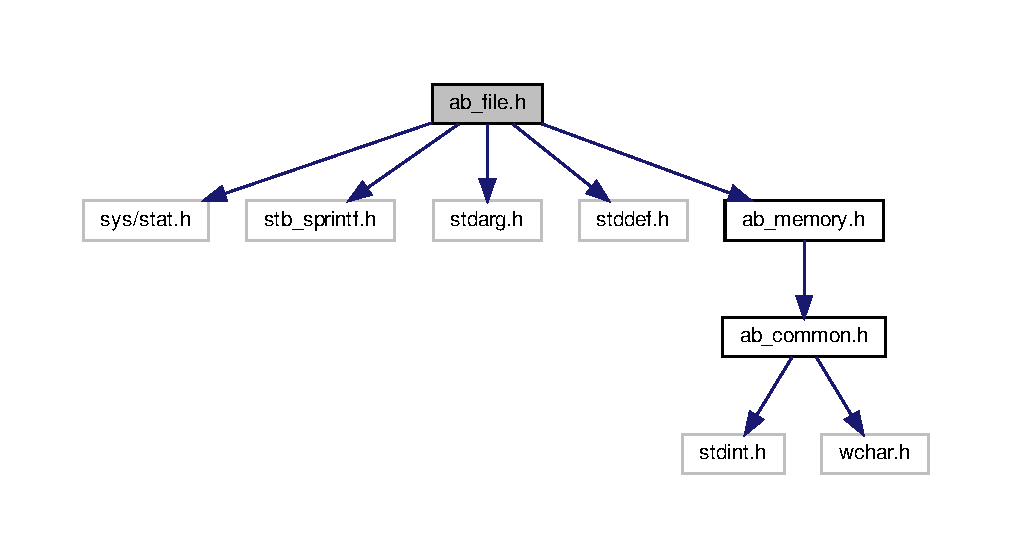
\includegraphics[width=350pt]{df/d58/ab__file_8h__incl}
\end{center}
\end{figure}
\subsection*{Classes}
\begin{DoxyCompactItemize}
\item 
struct \hyperlink{structfile__data}{file\+\_\+data}
\end{DoxyCompactItemize}
\subsection*{Macros}
\begin{DoxyCompactItemize}
\item 
\#define \hyperlink{ab__file_8h_ab99ded389af74001a6298fc9e44e74e5}{M\+A\+X\+\_\+\+P\+A\+TH}~255
\end{DoxyCompactItemize}
\subsection*{Enumerations}
\begin{DoxyCompactItemize}
\item 
enum \hyperlink{ab__file_8h_a1b665fc63cb310d53283fbcd1b19746e}{en\+File\+Type} \{ \hyperlink{ab__file_8h_a1b665fc63cb310d53283fbcd1b19746ea88183b946cc5f0e8c96b2e66e1c74a7e}{en\+File\+Type\+::\+Unknown}, 
\hyperlink{ab__file_8h_a1b665fc63cb310d53283fbcd1b19746eabf50d5e661106d0abe925af3c2e6f7e7}{en\+File\+Type\+::\+Header}, 
\hyperlink{ab__file_8h_a1b665fc63cb310d53283fbcd1b19746eadb4a39bf594c9fbcf318dd39ea19fed3}{en\+File\+Type\+::\+Cpp}
 \}
\end{DoxyCompactItemize}
\subsection*{Functions}
\begin{DoxyCompactItemize}
\item 
\hyperlink{ab__common_8h_a70e369648385b50f2d0588e8e8745275}{b8} \hyperlink{ab__file_8h_a4421ce1243877d8cc9082aae558db83f}{is\+Dir\+Exists} (const char $\ast$const path)
\item 
\hyperlink{structfile__list}{file\+\_\+list} $\ast$ \hyperlink{ab__file_8h_a3651116b0e04d2fdaedbe1154c22a46e}{abf\+\_\+\+Initialize\+File\+List} (\hyperlink{structmemory__arena}{memory\+\_\+arena} $\ast$Memory, const char $\ast$Path)
\item 
\hyperlink{ab__common_8h_a70e369648385b50f2d0588e8e8745275}{b8} \hyperlink{ab__file_8h_afba97cbbbebbd2066d87792952d894be}{abf\+\_\+\+Get\+Next\+File} (\hyperlink{structfile__list}{file\+\_\+list} $\ast$File\+List, \hyperlink{structfile__data}{file\+\_\+data} $\ast$File\+Data\+Out)
\item 
void \hyperlink{ab__file_8h_a4e85548dcb79723a8c6f468cf776826d}{abf\+\_\+\+Release\+File\+List} (\hyperlink{structfile__list}{file\+\_\+list} $\ast$File\+List)
\end{DoxyCompactItemize}


\subsection{Macro Definition Documentation}
\mbox{\Hypertarget{ab__file_8h_ab99ded389af74001a6298fc9e44e74e5}\label{ab__file_8h_ab99ded389af74001a6298fc9e44e74e5}} 
\index{ab\+\_\+file.\+h@{ab\+\_\+file.\+h}!M\+A\+X\+\_\+\+P\+A\+TH@{M\+A\+X\+\_\+\+P\+A\+TH}}
\index{M\+A\+X\+\_\+\+P\+A\+TH@{M\+A\+X\+\_\+\+P\+A\+TH}!ab\+\_\+file.\+h@{ab\+\_\+file.\+h}}
\subsubsection{\texorpdfstring{M\+A\+X\+\_\+\+P\+A\+TH}{MAX\_PATH}}
{\footnotesize\ttfamily \#define M\+A\+X\+\_\+\+P\+A\+TH~255}



\subsection{Enumeration Type Documentation}
\mbox{\Hypertarget{ab__file_8h_a1b665fc63cb310d53283fbcd1b19746e}\label{ab__file_8h_a1b665fc63cb310d53283fbcd1b19746e}} 
\index{ab\+\_\+file.\+h@{ab\+\_\+file.\+h}!en\+File\+Type@{en\+File\+Type}}
\index{en\+File\+Type@{en\+File\+Type}!ab\+\_\+file.\+h@{ab\+\_\+file.\+h}}
\subsubsection{\texorpdfstring{en\+File\+Type}{enFileType}}
{\footnotesize\ttfamily enum \hyperlink{ab__file_8h_a1b665fc63cb310d53283fbcd1b19746e}{en\+File\+Type}\hspace{0.3cm}{\ttfamily [strong]}}

\begin{DoxyEnumFields}{Enumerator}
\raisebox{\heightof{T}}[0pt][0pt]{\index{Unknown@{Unknown}!ab\+\_\+file.\+h@{ab\+\_\+file.\+h}}\index{ab\+\_\+file.\+h@{ab\+\_\+file.\+h}!Unknown@{Unknown}}}\mbox{\Hypertarget{ab__file_8h_a1b665fc63cb310d53283fbcd1b19746ea88183b946cc5f0e8c96b2e66e1c74a7e}\label{ab__file_8h_a1b665fc63cb310d53283fbcd1b19746ea88183b946cc5f0e8c96b2e66e1c74a7e}} 
Unknown&\\
\hline

\raisebox{\heightof{T}}[0pt][0pt]{\index{Header@{Header}!ab\+\_\+file.\+h@{ab\+\_\+file.\+h}}\index{ab\+\_\+file.\+h@{ab\+\_\+file.\+h}!Header@{Header}}}\mbox{\Hypertarget{ab__file_8h_a1b665fc63cb310d53283fbcd1b19746eabf50d5e661106d0abe925af3c2e6f7e7}\label{ab__file_8h_a1b665fc63cb310d53283fbcd1b19746eabf50d5e661106d0abe925af3c2e6f7e7}} 
Header&\\
\hline

\raisebox{\heightof{T}}[0pt][0pt]{\index{Cpp@{Cpp}!ab\+\_\+file.\+h@{ab\+\_\+file.\+h}}\index{ab\+\_\+file.\+h@{ab\+\_\+file.\+h}!Cpp@{Cpp}}}\mbox{\Hypertarget{ab__file_8h_a1b665fc63cb310d53283fbcd1b19746eadb4a39bf594c9fbcf318dd39ea19fed3}\label{ab__file_8h_a1b665fc63cb310d53283fbcd1b19746eadb4a39bf594c9fbcf318dd39ea19fed3}} 
Cpp&\\
\hline

\end{DoxyEnumFields}


\subsection{Function Documentation}
\mbox{\Hypertarget{ab__file_8h_afba97cbbbebbd2066d87792952d894be}\label{ab__file_8h_afba97cbbbebbd2066d87792952d894be}} 
\index{ab\+\_\+file.\+h@{ab\+\_\+file.\+h}!abf\+\_\+\+Get\+Next\+File@{abf\+\_\+\+Get\+Next\+File}}
\index{abf\+\_\+\+Get\+Next\+File@{abf\+\_\+\+Get\+Next\+File}!ab\+\_\+file.\+h@{ab\+\_\+file.\+h}}
\subsubsection{\texorpdfstring{abf\+\_\+\+Get\+Next\+File()}{abf\_GetNextFile()}}
{\footnotesize\ttfamily \hyperlink{ab__common_8h_a70e369648385b50f2d0588e8e8745275}{b8} abf\+\_\+\+Get\+Next\+File (\begin{DoxyParamCaption}\item[{\hyperlink{structfile__list}{file\+\_\+list} $\ast$}]{File\+List,  }\item[{\hyperlink{structfile__data}{file\+\_\+data} $\ast$}]{File\+Data\+Out }\end{DoxyParamCaption})}

\mbox{\Hypertarget{ab__file_8h_a3651116b0e04d2fdaedbe1154c22a46e}\label{ab__file_8h_a3651116b0e04d2fdaedbe1154c22a46e}} 
\index{ab\+\_\+file.\+h@{ab\+\_\+file.\+h}!abf\+\_\+\+Initialize\+File\+List@{abf\+\_\+\+Initialize\+File\+List}}
\index{abf\+\_\+\+Initialize\+File\+List@{abf\+\_\+\+Initialize\+File\+List}!ab\+\_\+file.\+h@{ab\+\_\+file.\+h}}
\subsubsection{\texorpdfstring{abf\+\_\+\+Initialize\+File\+List()}{abf\_InitializeFileList()}}
{\footnotesize\ttfamily \hyperlink{structfile__list}{file\+\_\+list}$\ast$ abf\+\_\+\+Initialize\+File\+List (\begin{DoxyParamCaption}\item[{\hyperlink{structmemory__arena}{memory\+\_\+arena} $\ast$}]{Memory,  }\item[{const char $\ast$}]{Path }\end{DoxyParamCaption})}

\mbox{\Hypertarget{ab__file_8h_a4e85548dcb79723a8c6f468cf776826d}\label{ab__file_8h_a4e85548dcb79723a8c6f468cf776826d}} 
\index{ab\+\_\+file.\+h@{ab\+\_\+file.\+h}!abf\+\_\+\+Release\+File\+List@{abf\+\_\+\+Release\+File\+List}}
\index{abf\+\_\+\+Release\+File\+List@{abf\+\_\+\+Release\+File\+List}!ab\+\_\+file.\+h@{ab\+\_\+file.\+h}}
\subsubsection{\texorpdfstring{abf\+\_\+\+Release\+File\+List()}{abf\_ReleaseFileList()}}
{\footnotesize\ttfamily void abf\+\_\+\+Release\+File\+List (\begin{DoxyParamCaption}\item[{\hyperlink{structfile__list}{file\+\_\+list} $\ast$}]{File\+List }\end{DoxyParamCaption})}

\mbox{\Hypertarget{ab__file_8h_a4421ce1243877d8cc9082aae558db83f}\label{ab__file_8h_a4421ce1243877d8cc9082aae558db83f}} 
\index{ab\+\_\+file.\+h@{ab\+\_\+file.\+h}!is\+Dir\+Exists@{is\+Dir\+Exists}}
\index{is\+Dir\+Exists@{is\+Dir\+Exists}!ab\+\_\+file.\+h@{ab\+\_\+file.\+h}}
\subsubsection{\texorpdfstring{is\+Dir\+Exists()}{isDirExists()}}
{\footnotesize\ttfamily \hyperlink{ab__common_8h_a70e369648385b50f2d0588e8e8745275}{b8} is\+Dir\+Exists (\begin{DoxyParamCaption}\item[{const char $\ast$const}]{path }\end{DoxyParamCaption})}


\hypertarget{ab__file__linux_8h}{}\doxysection{ab\+\_\+file\+\_\+linux.\+h File Reference}
\label{ab__file__linux_8h}\index{ab\_file\_linux.h@{ab\_file\_linux.h}}
{\ttfamily \#include $<$glob.\+h$>$}\newline
{\ttfamily \#include $<$sys/types.\+h$>$}\newline
{\ttfamily \#include $<$sys/stat.\+h$>$}\newline
{\ttfamily \#include $<$fcntl.\+h$>$}\newline
{\ttfamily \#include $<$unistd.\+h$>$}\newline
{\ttfamily \#include $<$malloc.\+h$>$}\newline
{\ttfamily \#include $<$libgen.\+h$>$}\newline
Include dependency graph for ab\+\_\+file\+\_\+linux.\+h\+:
\nopagebreak
\begin{figure}[H]
\begin{center}
\leavevmode
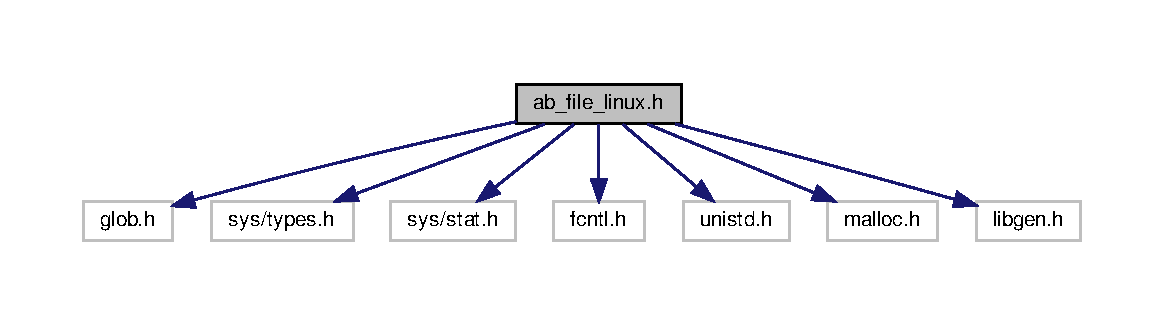
\includegraphics[width=350pt]{d3/d64/ab__file__linux_8h__incl}
\end{center}
\end{figure}
\doxysubsection*{Classes}
\begin{DoxyCompactItemize}
\item 
struct \mbox{\hyperlink{structfile__list}{file\+\_\+list}}
\end{DoxyCompactItemize}

\hypertarget{ab__file__win32_8h}{}\doxysection{ab\+\_\+file\+\_\+win32.\+h File Reference}
\label{ab__file__win32_8h}\index{ab\_file\_win32.h@{ab\_file\_win32.h}}


Windows specific implementation of some file functions.  


{\ttfamily \#include $<$windows.\+h$>$}\newline
{\ttfamily \#include $<$malloc.\+h$>$}\newline
{\ttfamily \#include \char`\"{}ab\+\_\+common.\+h\char`\"{}}\newline
{\ttfamily \#include \char`\"{}ab\+\_\+memory.\+h\char`\"{}}\newline
{\ttfamily \#include \char`\"{}ab\+\_\+string.\+h\char`\"{}}\newline
Include dependency graph for ab\+\_\+file\+\_\+win32.\+h\+:
\nopagebreak
\begin{figure}[H]
\begin{center}
\leavevmode
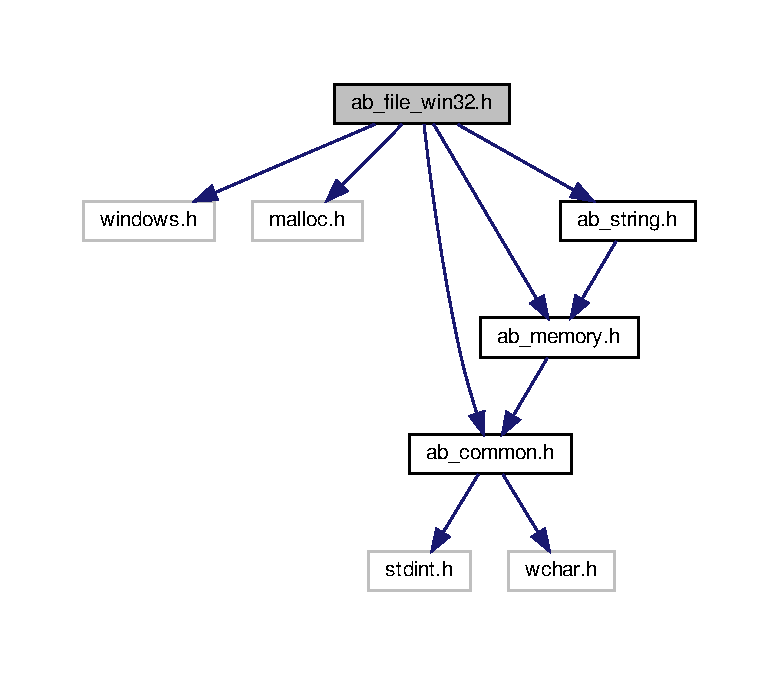
\includegraphics[width=350pt]{d8/d79/ab__file__win32_8h__incl}
\end{center}
\end{figure}
\doxysubsection*{Classes}
\begin{DoxyCompactItemize}
\item 
struct \mbox{\hyperlink{structfile__list}{file\+\_\+list}}
\end{DoxyCompactItemize}
\doxysubsection*{Macros}
\begin{DoxyCompactItemize}
\item 
\#define \mbox{\hyperlink{ab__file__win32_8h_ac7bef5d85e3dcd73eef56ad39ffc84a9}{W\+I\+N32\+\_\+\+L\+E\+A\+N\+\_\+\+A\+N\+D\+\_\+\+M\+E\+AN}}
\end{DoxyCompactItemize}


\doxysubsection{Detailed Description}
Windows specific implementation of some file functions. 

\begin{DoxyAuthor}{Author}
Amos Buchanan 
\end{DoxyAuthor}
\begin{DoxyVersion}{Version}
1.\+0 
\end{DoxyVersion}
\begin{DoxyDate}{Date}
2020 
\end{DoxyDate}
\begin{DoxyCopyright}{Copyright}
\href{https://opensource.org/licenses/MIT}{\texttt{ M\+IT Public License}}
\end{DoxyCopyright}
Windows specific implementation of functions. See \mbox{\hyperlink{ab__file_8h}{ab\+\_\+file.\+h}} for function usage.\hypertarget{ab__file__win32_8h_autotoc_md0}{}\doxysubsection{M\+I\+T License}\label{ab__file__win32_8h_autotoc_md0}
\href{https://opensource.org/licenses/MIT}{\texttt{ M\+IT Public License}}

Copyright 2020 Amos Buchanan

Permission is hereby granted, free of charge, to any person obtaining a copy of this software and associated documentation files (the \char`\"{}\+Software\char`\"{}), to deal in the Software without restriction, including without limitation the rights to use, copy, modify, merge, publish, distribute, sublicense, and/or sell copies of the Software, and to permit persons to whom the Software is furnished to do so, subject to the following conditions\+:

The above copyright notice and this permission notice shall be included in all copies or substantial portions of the Software.

T\+HE S\+O\+F\+T\+W\+A\+RE IS P\+R\+O\+V\+I\+D\+ED \char`\"{}\+A\+S I\+S\char`\"{}, W\+I\+T\+H\+O\+UT W\+A\+R\+R\+A\+N\+TY OF A\+NY K\+I\+ND, E\+X\+P\+R\+E\+SS OR I\+M\+P\+L\+I\+ED, I\+N\+C\+L\+U\+D\+I\+NG B\+UT N\+OT L\+I\+M\+I\+T\+ED TO T\+HE W\+A\+R\+R\+A\+N\+T\+I\+ES OF M\+E\+R\+C\+H\+A\+N\+T\+A\+B\+I\+L\+I\+TY, F\+I\+T\+N\+E\+SS F\+OR A P\+A\+R\+T\+I\+C\+U\+L\+AR P\+U\+R\+P\+O\+SE A\+ND N\+O\+N\+I\+N\+F\+R\+I\+N\+G\+E\+M\+E\+NT. IN NO E\+V\+E\+NT S\+H\+A\+LL T\+HE A\+U\+T\+H\+O\+RS OR C\+O\+P\+Y\+R\+I\+G\+HT H\+O\+L\+D\+E\+RS BE L\+I\+A\+B\+LE F\+OR A\+NY C\+L\+A\+IM, D\+A\+M\+A\+G\+ES OR O\+T\+H\+ER L\+I\+A\+B\+I\+L\+I\+TY, W\+H\+E\+T\+H\+ER IN AN A\+C\+T\+I\+ON OF C\+O\+N\+T\+R\+A\+CT, T\+O\+RT OR O\+T\+H\+E\+R\+W\+I\+SE, A\+R\+I\+S\+I\+NG F\+R\+OM, O\+UT OF OR IN C\+O\+N\+N\+E\+C\+T\+I\+ON W\+I\+TH T\+HE S\+O\+F\+T\+W\+A\+RE OR T\+HE U\+SE OR O\+T\+H\+ER D\+E\+A\+L\+I\+N\+GS IN T\+HE S\+O\+F\+T\+W\+A\+RE. 

\doxysubsection{Macro Definition Documentation}
\mbox{\Hypertarget{ab__file__win32_8h_ac7bef5d85e3dcd73eef56ad39ffc84a9}\label{ab__file__win32_8h_ac7bef5d85e3dcd73eef56ad39ffc84a9}} 
\index{ab\_file\_win32.h@{ab\_file\_win32.h}!WIN32\_LEAN\_AND\_MEAN@{WIN32\_LEAN\_AND\_MEAN}}
\index{WIN32\_LEAN\_AND\_MEAN@{WIN32\_LEAN\_AND\_MEAN}!ab\_file\_win32.h@{ab\_file\_win32.h}}
\doxysubsubsection{\texorpdfstring{WIN32\_LEAN\_AND\_MEAN}{WIN32\_LEAN\_AND\_MEAN}}
{\footnotesize\ttfamily \#define W\+I\+N32\+\_\+\+L\+E\+A\+N\+\_\+\+A\+N\+D\+\_\+\+M\+E\+AN}


\hypertarget{ab__json_8h}{}\section{ab\+\_\+json.\+h File Reference}
\label{ab__json_8h}\index{ab\+\_\+json.\+h@{ab\+\_\+json.\+h}}
{\ttfamily \#include \char`\"{}ab\+\_\+common.\+h\char`\"{}}\newline
{\ttfamily \#include \char`\"{}ab\+\_\+memory.\+h\char`\"{}}\newline
{\ttfamily \#include \char`\"{}ab\+\_\+string.\+h\char`\"{}}\newline
{\ttfamily \#include \char`\"{}jsmn.\+h\char`\"{}}\newline
Include dependency graph for ab\+\_\+json.\+h\+:\nopagebreak
\begin{figure}[H]
\begin{center}
\leavevmode
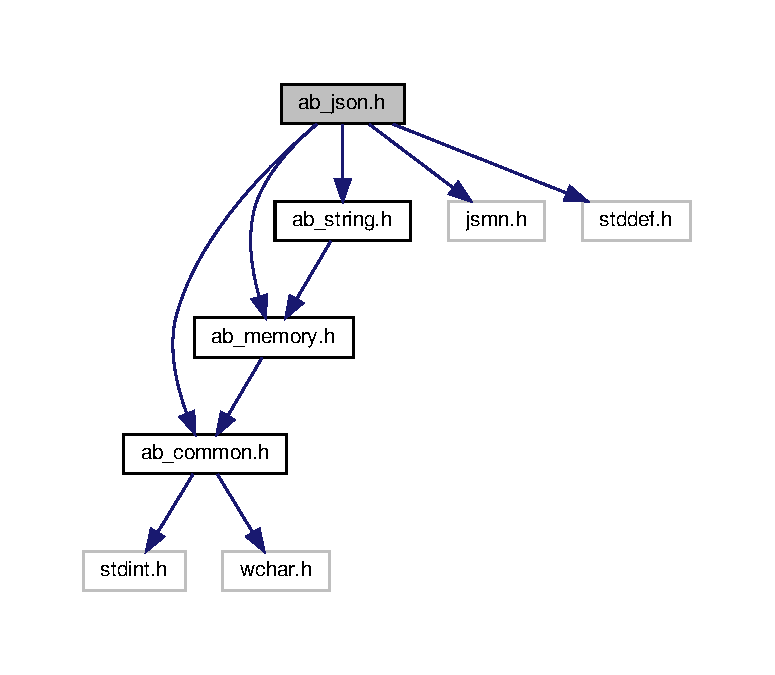
\includegraphics[width=305pt]{d2/d00/ab__json_8h__incl}
\end{center}
\end{figure}
This graph shows which files directly or indirectly include this file\+:\nopagebreak
\begin{figure}[H]
\begin{center}
\leavevmode
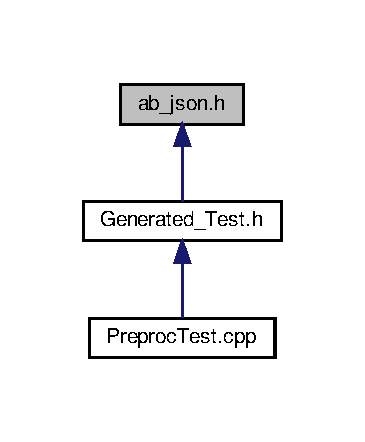
\includegraphics[width=175pt]{d5/d2e/ab__json_8h__dep__incl}
\end{center}
\end{figure}
\subsection*{Macros}
\begin{DoxyCompactItemize}
\item 
\#define \hyperlink{ab__json_8h_aeef9c3539ffb9ed912a2976b67b43d68}{J\+S\+M\+N\+\_\+\+H\+E\+A\+D\+ER}
\end{DoxyCompactItemize}
\subsection*{Enumerations}
\begin{DoxyCompactItemize}
\item 
enum \hyperlink{ab__json_8h_a23451be0e28c552e70c19429684f83cb}{json\+\_\+flags} \{ \hyperlink{ab__json_8h_a23451be0e28c552e70c19429684f83cba12d51163882c2f3f659bf2d2560969b6}{J\+S\+O\+N\+\_\+\+Null} = 0, 
\hyperlink{ab__json_8h_a23451be0e28c552e70c19429684f83cbab892e8229f95855a30a2c10fde71f78e}{J\+S\+O\+N\+\_\+\+Is\+Last\+In\+List} = 1 $<$$<$ 0, 
\hyperlink{ab__json_8h_a23451be0e28c552e70c19429684f83cba4f2bc16d9f2cb38d0e0354342bcd07c1}{J\+S\+O\+N\+\_\+\+Dont\+Use\+Tag} = 1 $<$$<$ 1, 
\hyperlink{ab__json_8h_a23451be0e28c552e70c19429684f83cba508ef51fa6f4677dd0ba7b242f0d269f}{J\+S\+O\+N\+\_\+\+Base\+Object} = 1 $<$$<$ 2
 \}
\end{DoxyCompactItemize}
\subsection*{Functions}
\begin{DoxyCompactItemize}
\item 
\hyperlink{ab__common_8h_ae9b1af5c037e57a98884758875d3a7c4}{s32} \hyperlink{ab__json_8h_a2b3b6ac206a0ad8367ef1b795ae06d94}{Parse\+Json} (\hyperlink{structmemory__arena}{memory\+\_\+arena} $\ast$Volatile\+Memory, char const $\ast$Json, size\+\_\+t Json\+Length, \hyperlink{structjsmntok__t}{jsmntok\+\_\+t} $\ast$$\ast$Token\+Array)
\item 
\hyperlink{ab__common_8h_afaa62991928fb9fb18ff0db62a040aba}{u32} \hyperlink{ab__json_8h_a2c85de19a5702595393c516b1637896b}{Start\+Group} (char $\ast$, \hyperlink{ab__common_8h_afaa62991928fb9fb18ff0db62a040aba}{u32} Max\+Length)
\item 
\hyperlink{ab__common_8h_afaa62991928fb9fb18ff0db62a040aba}{u32} \hyperlink{ab__json_8h_a8d4a5895fda267713cbb9818d27e1a57}{End\+Group} (char $\ast$, \hyperlink{ab__common_8h_afaa62991928fb9fb18ff0db62a040aba}{u32} Max\+Length, \hyperlink{ab__common_8h_a70e369648385b50f2d0588e8e8745275}{b8} is\+Last)
\item 
\hyperlink{structabs__stringptr}{abs\+\_\+stringptr} \hyperlink{ab__json_8h_a6d809a2544db46f751036c308b9ec380}{Token\+To\+String\+Ptr} (char const $\ast$Json, \hyperlink{structjsmntok__t}{jsmntok\+\_\+t} $\ast$Token)
\item 
\hyperlink{ab__common_8h_a70e369648385b50f2d0588e8e8745275}{b8} \hyperlink{ab__json_8h_adc0dbd5f4b093577ebd0b4e252e17731}{Token\+Equals} (char const $\ast$Json, \hyperlink{structjsmntok__t}{jsmntok\+\_\+t} $\ast$Token, char const $\ast$Value)
\end{DoxyCompactItemize}


\subsection{Macro Definition Documentation}
\mbox{\Hypertarget{ab__json_8h_aeef9c3539ffb9ed912a2976b67b43d68}\label{ab__json_8h_aeef9c3539ffb9ed912a2976b67b43d68}} 
\index{ab\+\_\+json.\+h@{ab\+\_\+json.\+h}!J\+S\+M\+N\+\_\+\+H\+E\+A\+D\+ER@{J\+S\+M\+N\+\_\+\+H\+E\+A\+D\+ER}}
\index{J\+S\+M\+N\+\_\+\+H\+E\+A\+D\+ER@{J\+S\+M\+N\+\_\+\+H\+E\+A\+D\+ER}!ab\+\_\+json.\+h@{ab\+\_\+json.\+h}}
\subsubsection{\texorpdfstring{J\+S\+M\+N\+\_\+\+H\+E\+A\+D\+ER}{JSMN\_HEADER}}
{\footnotesize\ttfamily \#define J\+S\+M\+N\+\_\+\+H\+E\+A\+D\+ER}



\subsection{Enumeration Type Documentation}
\mbox{\Hypertarget{ab__json_8h_a23451be0e28c552e70c19429684f83cb}\label{ab__json_8h_a23451be0e28c552e70c19429684f83cb}} 
\index{ab\+\_\+json.\+h@{ab\+\_\+json.\+h}!json\+\_\+flags@{json\+\_\+flags}}
\index{json\+\_\+flags@{json\+\_\+flags}!ab\+\_\+json.\+h@{ab\+\_\+json.\+h}}
\subsubsection{\texorpdfstring{json\+\_\+flags}{json\_flags}}
{\footnotesize\ttfamily enum \hyperlink{ab__json_8h_a23451be0e28c552e70c19429684f83cb}{json\+\_\+flags}}

\begin{DoxyEnumFields}{Enumerator}
\raisebox{\heightof{T}}[0pt][0pt]{\index{J\+S\+O\+N\+\_\+\+Null@{J\+S\+O\+N\+\_\+\+Null}!ab\+\_\+json.\+h@{ab\+\_\+json.\+h}}\index{ab\+\_\+json.\+h@{ab\+\_\+json.\+h}!J\+S\+O\+N\+\_\+\+Null@{J\+S\+O\+N\+\_\+\+Null}}}\mbox{\Hypertarget{ab__json_8h_a23451be0e28c552e70c19429684f83cba12d51163882c2f3f659bf2d2560969b6}\label{ab__json_8h_a23451be0e28c552e70c19429684f83cba12d51163882c2f3f659bf2d2560969b6}} 
J\+S\+O\+N\+\_\+\+Null&\\
\hline

\raisebox{\heightof{T}}[0pt][0pt]{\index{J\+S\+O\+N\+\_\+\+Is\+Last\+In\+List@{J\+S\+O\+N\+\_\+\+Is\+Last\+In\+List}!ab\+\_\+json.\+h@{ab\+\_\+json.\+h}}\index{ab\+\_\+json.\+h@{ab\+\_\+json.\+h}!J\+S\+O\+N\+\_\+\+Is\+Last\+In\+List@{J\+S\+O\+N\+\_\+\+Is\+Last\+In\+List}}}\mbox{\Hypertarget{ab__json_8h_a23451be0e28c552e70c19429684f83cbab892e8229f95855a30a2c10fde71f78e}\label{ab__json_8h_a23451be0e28c552e70c19429684f83cbab892e8229f95855a30a2c10fde71f78e}} 
J\+S\+O\+N\+\_\+\+Is\+Last\+In\+List&\\
\hline

\raisebox{\heightof{T}}[0pt][0pt]{\index{J\+S\+O\+N\+\_\+\+Dont\+Use\+Tag@{J\+S\+O\+N\+\_\+\+Dont\+Use\+Tag}!ab\+\_\+json.\+h@{ab\+\_\+json.\+h}}\index{ab\+\_\+json.\+h@{ab\+\_\+json.\+h}!J\+S\+O\+N\+\_\+\+Dont\+Use\+Tag@{J\+S\+O\+N\+\_\+\+Dont\+Use\+Tag}}}\mbox{\Hypertarget{ab__json_8h_a23451be0e28c552e70c19429684f83cba4f2bc16d9f2cb38d0e0354342bcd07c1}\label{ab__json_8h_a23451be0e28c552e70c19429684f83cba4f2bc16d9f2cb38d0e0354342bcd07c1}} 
J\+S\+O\+N\+\_\+\+Dont\+Use\+Tag&\\
\hline

\raisebox{\heightof{T}}[0pt][0pt]{\index{J\+S\+O\+N\+\_\+\+Base\+Object@{J\+S\+O\+N\+\_\+\+Base\+Object}!ab\+\_\+json.\+h@{ab\+\_\+json.\+h}}\index{ab\+\_\+json.\+h@{ab\+\_\+json.\+h}!J\+S\+O\+N\+\_\+\+Base\+Object@{J\+S\+O\+N\+\_\+\+Base\+Object}}}\mbox{\Hypertarget{ab__json_8h_a23451be0e28c552e70c19429684f83cba508ef51fa6f4677dd0ba7b242f0d269f}\label{ab__json_8h_a23451be0e28c552e70c19429684f83cba508ef51fa6f4677dd0ba7b242f0d269f}} 
J\+S\+O\+N\+\_\+\+Base\+Object&\\
\hline

\end{DoxyEnumFields}


\subsection{Function Documentation}
\mbox{\Hypertarget{ab__json_8h_a8d4a5895fda267713cbb9818d27e1a57}\label{ab__json_8h_a8d4a5895fda267713cbb9818d27e1a57}} 
\index{ab\+\_\+json.\+h@{ab\+\_\+json.\+h}!End\+Group@{End\+Group}}
\index{End\+Group@{End\+Group}!ab\+\_\+json.\+h@{ab\+\_\+json.\+h}}
\subsubsection{\texorpdfstring{End\+Group()}{EndGroup()}}
{\footnotesize\ttfamily \hyperlink{ab__common_8h_afaa62991928fb9fb18ff0db62a040aba}{u32} End\+Group (\begin{DoxyParamCaption}\item[{char $\ast$}]{,  }\item[{\hyperlink{ab__common_8h_afaa62991928fb9fb18ff0db62a040aba}{u32}}]{Max\+Length,  }\item[{\hyperlink{ab__common_8h_a70e369648385b50f2d0588e8e8745275}{b8}}]{is\+Last }\end{DoxyParamCaption})\hspace{0.3cm}{\ttfamily [inline]}}

\mbox{\Hypertarget{ab__json_8h_a2b3b6ac206a0ad8367ef1b795ae06d94}\label{ab__json_8h_a2b3b6ac206a0ad8367ef1b795ae06d94}} 
\index{ab\+\_\+json.\+h@{ab\+\_\+json.\+h}!Parse\+Json@{Parse\+Json}}
\index{Parse\+Json@{Parse\+Json}!ab\+\_\+json.\+h@{ab\+\_\+json.\+h}}
\subsubsection{\texorpdfstring{Parse\+Json()}{ParseJson()}}
{\footnotesize\ttfamily \hyperlink{ab__common_8h_ae9b1af5c037e57a98884758875d3a7c4}{s32} Parse\+Json (\begin{DoxyParamCaption}\item[{\hyperlink{structmemory__arena}{memory\+\_\+arena} $\ast$}]{Volatile\+Memory,  }\item[{char const $\ast$}]{Json,  }\item[{size\+\_\+t}]{Json\+Length,  }\item[{\hyperlink{structjsmntok__t}{jsmntok\+\_\+t} $\ast$$\ast$}]{Token\+Array }\end{DoxyParamCaption})\hspace{0.3cm}{\ttfamily [inline]}}

\mbox{\Hypertarget{ab__json_8h_a2c85de19a5702595393c516b1637896b}\label{ab__json_8h_a2c85de19a5702595393c516b1637896b}} 
\index{ab\+\_\+json.\+h@{ab\+\_\+json.\+h}!Start\+Group@{Start\+Group}}
\index{Start\+Group@{Start\+Group}!ab\+\_\+json.\+h@{ab\+\_\+json.\+h}}
\subsubsection{\texorpdfstring{Start\+Group()}{StartGroup()}}
{\footnotesize\ttfamily \hyperlink{ab__common_8h_afaa62991928fb9fb18ff0db62a040aba}{u32} Start\+Group (\begin{DoxyParamCaption}\item[{char $\ast$}]{,  }\item[{\hyperlink{ab__common_8h_afaa62991928fb9fb18ff0db62a040aba}{u32}}]{Max\+Length }\end{DoxyParamCaption})\hspace{0.3cm}{\ttfamily [inline]}}

\mbox{\Hypertarget{ab__json_8h_adc0dbd5f4b093577ebd0b4e252e17731}\label{ab__json_8h_adc0dbd5f4b093577ebd0b4e252e17731}} 
\index{ab\+\_\+json.\+h@{ab\+\_\+json.\+h}!Token\+Equals@{Token\+Equals}}
\index{Token\+Equals@{Token\+Equals}!ab\+\_\+json.\+h@{ab\+\_\+json.\+h}}
\subsubsection{\texorpdfstring{Token\+Equals()}{TokenEquals()}}
{\footnotesize\ttfamily \hyperlink{ab__common_8h_a70e369648385b50f2d0588e8e8745275}{b8} Token\+Equals (\begin{DoxyParamCaption}\item[{char const $\ast$}]{Json,  }\item[{\hyperlink{structjsmntok__t}{jsmntok\+\_\+t} $\ast$}]{Token,  }\item[{char const $\ast$}]{Value }\end{DoxyParamCaption})\hspace{0.3cm}{\ttfamily [inline]}}

\mbox{\Hypertarget{ab__json_8h_a6d809a2544db46f751036c308b9ec380}\label{ab__json_8h_a6d809a2544db46f751036c308b9ec380}} 
\index{ab\+\_\+json.\+h@{ab\+\_\+json.\+h}!Token\+To\+String\+Ptr@{Token\+To\+String\+Ptr}}
\index{Token\+To\+String\+Ptr@{Token\+To\+String\+Ptr}!ab\+\_\+json.\+h@{ab\+\_\+json.\+h}}
\subsubsection{\texorpdfstring{Token\+To\+String\+Ptr()}{TokenToStringPtr()}}
{\footnotesize\ttfamily \hyperlink{structabs__stringptr}{abs\+\_\+stringptr} Token\+To\+String\+Ptr (\begin{DoxyParamCaption}\item[{char const $\ast$}]{Json,  }\item[{\hyperlink{structjsmntok__t}{jsmntok\+\_\+t} $\ast$}]{Token }\end{DoxyParamCaption})\hspace{0.3cm}{\ttfamily [inline]}}


\hypertarget{ab__lexer_8h}{}\doxysection{ab\+\_\+lexer.\+h File Reference}
\label{ab__lexer_8h}\index{ab\_lexer.h@{ab\_lexer.h}}
{\ttfamily \#include $<$stdlib.\+h$>$}\newline
{\ttfamily \#include \char`\"{}ab\+\_\+string.\+h\char`\"{}}\newline
{\ttfamily \#include \char`\"{}ab\+\_\+file.\+h\char`\"{}}\newline
Include dependency graph for ab\+\_\+lexer.\+h\+:
\nopagebreak
\begin{figure}[H]
\begin{center}
\leavevmode
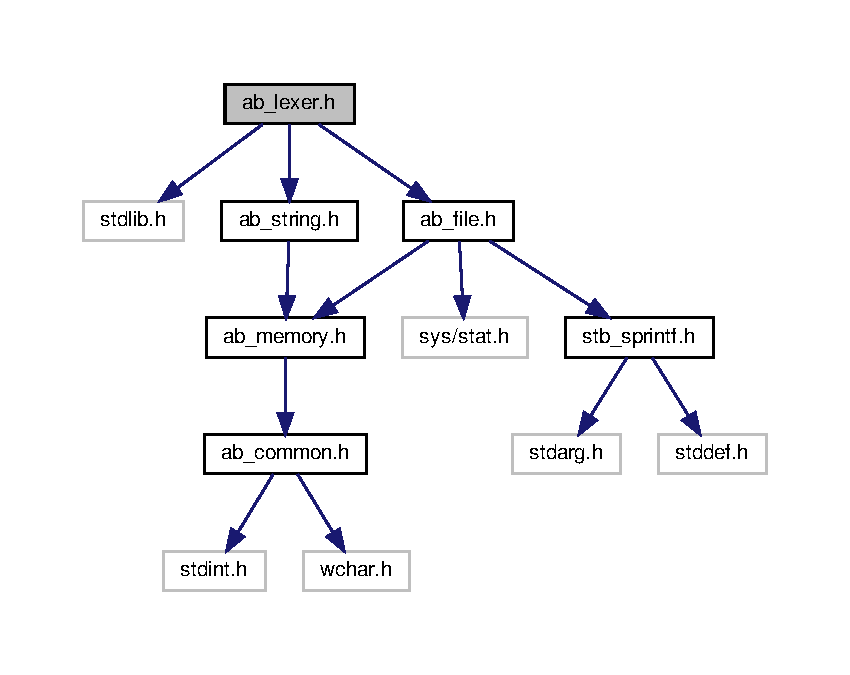
\includegraphics[width=350pt]{da/d7a/ab__lexer_8h__incl}
\end{center}
\end{figure}
This graph shows which files directly or indirectly include this file\+:
\nopagebreak
\begin{figure}[H]
\begin{center}
\leavevmode
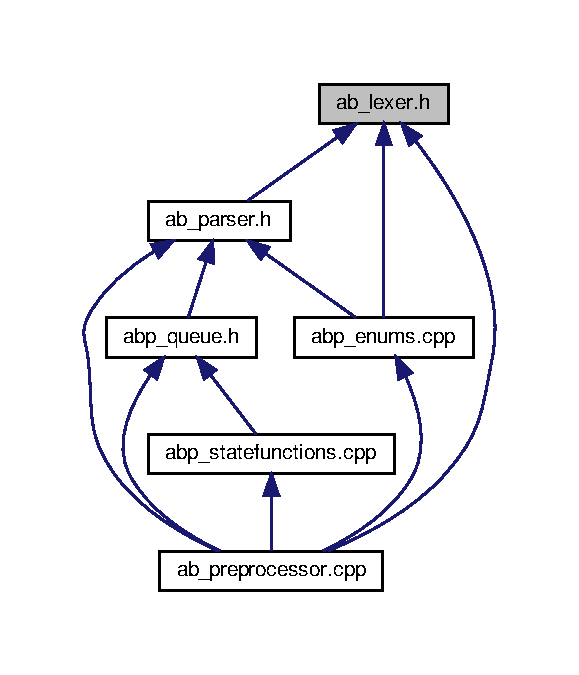
\includegraphics[width=350pt]{d7/d69/ab__lexer_8h__dep__incl}
\end{center}
\end{figure}
\doxysubsection*{Classes}
\begin{DoxyCompactItemize}
\item 
struct \mbox{\hyperlink{structtoken}{token}}
\item 
struct \mbox{\hyperlink{structlexer}{lexer}}
\end{DoxyCompactItemize}
\doxysubsection*{Enumerations}
\begin{DoxyCompactItemize}
\item 
enum \mbox{\hyperlink{ab__lexer_8h_afe5ef662303b6b710ea6ee1a944bad0d}{token\+\_\+type}} \{ \newline
\mbox{\hyperlink{ab__lexer_8h_afe5ef662303b6b710ea6ee1a944bad0da892829e561dc7befd1a48886ec9fafaf}{T\+O\+K\+E\+N\+\_\+\+Unknown}}, 
\mbox{\hyperlink{ab__lexer_8h_afe5ef662303b6b710ea6ee1a944bad0da461b56860fa20c58692816c64fbe3e82}{T\+O\+K\+E\+N\+\_\+\+Open\+Paren}}, 
\mbox{\hyperlink{ab__lexer_8h_afe5ef662303b6b710ea6ee1a944bad0dab194bde3d5b9eedc596b4e9c177a02bf}{T\+O\+K\+E\+N\+\_\+\+Close\+Paren}}, 
\mbox{\hyperlink{ab__lexer_8h_afe5ef662303b6b710ea6ee1a944bad0da844de61fbecc86df7402533595d0028e}{T\+O\+K\+E\+N\+\_\+\+Colon}}, 
\newline
\mbox{\hyperlink{ab__lexer_8h_afe5ef662303b6b710ea6ee1a944bad0da1e561e7c4db683063f655b59f48d8fa1}{T\+O\+K\+E\+N\+\_\+\+Semicolon}}, 
\mbox{\hyperlink{ab__lexer_8h_afe5ef662303b6b710ea6ee1a944bad0dad6aae4a41409c1b9e0ea73cc0896843b}{T\+O\+K\+E\+N\+\_\+\+Comma}}, 
\mbox{\hyperlink{ab__lexer_8h_afe5ef662303b6b710ea6ee1a944bad0da15a0aa1b1e93135757584ccd08634c5c}{T\+O\+K\+E\+N\+\_\+\+Asterisk}}, 
\mbox{\hyperlink{ab__lexer_8h_afe5ef662303b6b710ea6ee1a944bad0dafd406f033139bb6f609ace25a31c2f3a}{T\+O\+K\+E\+N\+\_\+\+Open\+Bracket}}, 
\newline
\mbox{\hyperlink{ab__lexer_8h_afe5ef662303b6b710ea6ee1a944bad0da3be38f6d9101f2361ffb117bde66e8b1}{T\+O\+K\+E\+N\+\_\+\+Close\+Bracket}}, 
\mbox{\hyperlink{ab__lexer_8h_afe5ef662303b6b710ea6ee1a944bad0da985f18bfc75b5bb16f6d8cd7ee3c5eef}{T\+O\+K\+E\+N\+\_\+\+Open\+Brace}}, 
\mbox{\hyperlink{ab__lexer_8h_afe5ef662303b6b710ea6ee1a944bad0da00140195c489d01ef4834626b6b228b2}{T\+O\+K\+E\+N\+\_\+\+Close\+Brace}}, 
\mbox{\hyperlink{ab__lexer_8h_afe5ef662303b6b710ea6ee1a944bad0daa49eebd79816e15da448344906a2c89a}{T\+O\+K\+E\+N\+\_\+\+Dollar}}, 
\newline
\mbox{\hyperlink{ab__lexer_8h_afe5ef662303b6b710ea6ee1a944bad0da6785e5266e9a8f26117eec7c9031988f}{T\+O\+K\+E\+N\+\_\+\+Backslash}}, 
\mbox{\hyperlink{ab__lexer_8h_afe5ef662303b6b710ea6ee1a944bad0da537e6fab007d5fad82eb3dc17a03ac5f}{T\+O\+K\+E\+N\+\_\+\+Foreslash}}, 
\mbox{\hyperlink{ab__lexer_8h_afe5ef662303b6b710ea6ee1a944bad0dabc77e1fd3b2968061292389175c85f9d}{T\+O\+K\+E\+N\+\_\+\+Ampersand}}, 
\mbox{\hyperlink{ab__lexer_8h_afe5ef662303b6b710ea6ee1a944bad0dab3ab21eb59569f77e5a760b60450ca88}{T\+O\+K\+E\+N\+\_\+\+Pound}}, 
\newline
\mbox{\hyperlink{ab__lexer_8h_afe5ef662303b6b710ea6ee1a944bad0da193eb7659e6c00986e0aff62dbbeb09d}{T\+O\+K\+E\+N\+\_\+\+String}}, 
\mbox{\hyperlink{ab__lexer_8h_afe5ef662303b6b710ea6ee1a944bad0da0d4578db72362887dfde5f1cd25d55be}{T\+O\+K\+E\+N\+\_\+\+Identifier}}, 
\mbox{\hyperlink{ab__lexer_8h_afe5ef662303b6b710ea6ee1a944bad0da7ed6181a144b374be16cf530d848e37f}{T\+O\+K\+E\+N\+\_\+\+Number}}, 
\mbox{\hyperlink{ab__lexer_8h_afe5ef662303b6b710ea6ee1a944bad0da5ea8b7dc749074b9d0bcb9c6bb4b371a}{T\+O\+K\+E\+N\+\_\+\+End\+Of\+Stream}}, 
\newline
\mbox{\hyperlink{ab__lexer_8h_afe5ef662303b6b710ea6ee1a944bad0daed656b1d460c6ef81c68df705a2f5078}{T\+O\+K\+E\+N\+\_\+\+Count}}
 \}
\end{DoxyCompactItemize}
\doxysubsection*{Functions}
\begin{DoxyCompactItemize}
\item 
void \mbox{\hyperlink{ab__lexer_8h_ac5eb995db6ef91a2911edacd008016fe}{abl\+\_\+\+Init\+Lexer}} (\mbox{\hyperlink{structlexer}{lexer}} $\ast$Lexer, \mbox{\hyperlink{structfile__data}{file\+\_\+data}} $\ast$File)
\item 
\mbox{\hyperlink{structtoken}{token}} \mbox{\hyperlink{ab__lexer_8h_a0274c02cba41dfe765ef9daa141c9f95}{abl\+\_\+\+Get\+Token}} (\mbox{\hyperlink{structlexer}{lexer}} $\ast$Lexer)
\item 
\mbox{\hyperlink{structtoken}{token}} \mbox{\hyperlink{ab__lexer_8h_a1aa9628424ed3855b5c1680d0cd15b67}{abl\+\_\+\+Peek\+Token}} (\mbox{\hyperlink{structlexer}{lexer}} $\ast$Lexer)
\item 
s32 \mbox{\hyperlink{ab__lexer_8h_abcfa4b95aa0c3903a1a16e72163d6d64}{abl\+\_\+\+Token\+To\+S32}} (\mbox{\hyperlink{structtoken}{token}} Token)
\item 
b8 \mbox{\hyperlink{ab__lexer_8h_aa3038ae93cd0f42ca4214c070243c8bb}{abl\+\_\+\+Token\+Equals}} (\mbox{\hyperlink{structtoken}{token}} Token, abs\+\_\+stringptr Match)
\item 
b8 \mbox{\hyperlink{ab__lexer_8h_a1552415fbb937ff170b11b756b5519bc}{abl\+\_\+\+Tokens\+Equals}} (\mbox{\hyperlink{structtoken}{token}} A, \mbox{\hyperlink{structtoken}{token}} B)
\end{DoxyCompactItemize}


\doxysubsection{Enumeration Type Documentation}
\mbox{\Hypertarget{ab__lexer_8h_afe5ef662303b6b710ea6ee1a944bad0d}\label{ab__lexer_8h_afe5ef662303b6b710ea6ee1a944bad0d}} 
\index{ab\_lexer.h@{ab\_lexer.h}!token\_type@{token\_type}}
\index{token\_type@{token\_type}!ab\_lexer.h@{ab\_lexer.h}}
\doxysubsubsection{\texorpdfstring{token\_type}{token\_type}}
{\footnotesize\ttfamily enum \mbox{\hyperlink{ab__lexer_8h_afe5ef662303b6b710ea6ee1a944bad0d}{token\+\_\+type}}}

\begin{DoxyEnumFields}{Enumerator}
\raisebox{\heightof{T}}[0pt][0pt]{\index{TOKEN\_Unknown@{TOKEN\_Unknown}!ab\_lexer.h@{ab\_lexer.h}}\index{ab\_lexer.h@{ab\_lexer.h}!TOKEN\_Unknown@{TOKEN\_Unknown}}}\mbox{\Hypertarget{ab__lexer_8h_afe5ef662303b6b710ea6ee1a944bad0da892829e561dc7befd1a48886ec9fafaf}\label{ab__lexer_8h_afe5ef662303b6b710ea6ee1a944bad0da892829e561dc7befd1a48886ec9fafaf}} 
T\+O\+K\+E\+N\+\_\+\+Unknown&\\
\hline

\raisebox{\heightof{T}}[0pt][0pt]{\index{TOKEN\_OpenParen@{TOKEN\_OpenParen}!ab\_lexer.h@{ab\_lexer.h}}\index{ab\_lexer.h@{ab\_lexer.h}!TOKEN\_OpenParen@{TOKEN\_OpenParen}}}\mbox{\Hypertarget{ab__lexer_8h_afe5ef662303b6b710ea6ee1a944bad0da461b56860fa20c58692816c64fbe3e82}\label{ab__lexer_8h_afe5ef662303b6b710ea6ee1a944bad0da461b56860fa20c58692816c64fbe3e82}} 
T\+O\+K\+E\+N\+\_\+\+Open\+Paren&\\
\hline

\raisebox{\heightof{T}}[0pt][0pt]{\index{TOKEN\_CloseParen@{TOKEN\_CloseParen}!ab\_lexer.h@{ab\_lexer.h}}\index{ab\_lexer.h@{ab\_lexer.h}!TOKEN\_CloseParen@{TOKEN\_CloseParen}}}\mbox{\Hypertarget{ab__lexer_8h_afe5ef662303b6b710ea6ee1a944bad0dab194bde3d5b9eedc596b4e9c177a02bf}\label{ab__lexer_8h_afe5ef662303b6b710ea6ee1a944bad0dab194bde3d5b9eedc596b4e9c177a02bf}} 
T\+O\+K\+E\+N\+\_\+\+Close\+Paren&\\
\hline

\raisebox{\heightof{T}}[0pt][0pt]{\index{TOKEN\_Colon@{TOKEN\_Colon}!ab\_lexer.h@{ab\_lexer.h}}\index{ab\_lexer.h@{ab\_lexer.h}!TOKEN\_Colon@{TOKEN\_Colon}}}\mbox{\Hypertarget{ab__lexer_8h_afe5ef662303b6b710ea6ee1a944bad0da844de61fbecc86df7402533595d0028e}\label{ab__lexer_8h_afe5ef662303b6b710ea6ee1a944bad0da844de61fbecc86df7402533595d0028e}} 
T\+O\+K\+E\+N\+\_\+\+Colon&\\
\hline

\raisebox{\heightof{T}}[0pt][0pt]{\index{TOKEN\_Semicolon@{TOKEN\_Semicolon}!ab\_lexer.h@{ab\_lexer.h}}\index{ab\_lexer.h@{ab\_lexer.h}!TOKEN\_Semicolon@{TOKEN\_Semicolon}}}\mbox{\Hypertarget{ab__lexer_8h_afe5ef662303b6b710ea6ee1a944bad0da1e561e7c4db683063f655b59f48d8fa1}\label{ab__lexer_8h_afe5ef662303b6b710ea6ee1a944bad0da1e561e7c4db683063f655b59f48d8fa1}} 
T\+O\+K\+E\+N\+\_\+\+Semicolon&\\
\hline

\raisebox{\heightof{T}}[0pt][0pt]{\index{TOKEN\_Comma@{TOKEN\_Comma}!ab\_lexer.h@{ab\_lexer.h}}\index{ab\_lexer.h@{ab\_lexer.h}!TOKEN\_Comma@{TOKEN\_Comma}}}\mbox{\Hypertarget{ab__lexer_8h_afe5ef662303b6b710ea6ee1a944bad0dad6aae4a41409c1b9e0ea73cc0896843b}\label{ab__lexer_8h_afe5ef662303b6b710ea6ee1a944bad0dad6aae4a41409c1b9e0ea73cc0896843b}} 
T\+O\+K\+E\+N\+\_\+\+Comma&\\
\hline

\raisebox{\heightof{T}}[0pt][0pt]{\index{TOKEN\_Asterisk@{TOKEN\_Asterisk}!ab\_lexer.h@{ab\_lexer.h}}\index{ab\_lexer.h@{ab\_lexer.h}!TOKEN\_Asterisk@{TOKEN\_Asterisk}}}\mbox{\Hypertarget{ab__lexer_8h_afe5ef662303b6b710ea6ee1a944bad0da15a0aa1b1e93135757584ccd08634c5c}\label{ab__lexer_8h_afe5ef662303b6b710ea6ee1a944bad0da15a0aa1b1e93135757584ccd08634c5c}} 
T\+O\+K\+E\+N\+\_\+\+Asterisk&\\
\hline

\raisebox{\heightof{T}}[0pt][0pt]{\index{TOKEN\_OpenBracket@{TOKEN\_OpenBracket}!ab\_lexer.h@{ab\_lexer.h}}\index{ab\_lexer.h@{ab\_lexer.h}!TOKEN\_OpenBracket@{TOKEN\_OpenBracket}}}\mbox{\Hypertarget{ab__lexer_8h_afe5ef662303b6b710ea6ee1a944bad0dafd406f033139bb6f609ace25a31c2f3a}\label{ab__lexer_8h_afe5ef662303b6b710ea6ee1a944bad0dafd406f033139bb6f609ace25a31c2f3a}} 
T\+O\+K\+E\+N\+\_\+\+Open\+Bracket&\\
\hline

\raisebox{\heightof{T}}[0pt][0pt]{\index{TOKEN\_CloseBracket@{TOKEN\_CloseBracket}!ab\_lexer.h@{ab\_lexer.h}}\index{ab\_lexer.h@{ab\_lexer.h}!TOKEN\_CloseBracket@{TOKEN\_CloseBracket}}}\mbox{\Hypertarget{ab__lexer_8h_afe5ef662303b6b710ea6ee1a944bad0da3be38f6d9101f2361ffb117bde66e8b1}\label{ab__lexer_8h_afe5ef662303b6b710ea6ee1a944bad0da3be38f6d9101f2361ffb117bde66e8b1}} 
T\+O\+K\+E\+N\+\_\+\+Close\+Bracket&\\
\hline

\raisebox{\heightof{T}}[0pt][0pt]{\index{TOKEN\_OpenBrace@{TOKEN\_OpenBrace}!ab\_lexer.h@{ab\_lexer.h}}\index{ab\_lexer.h@{ab\_lexer.h}!TOKEN\_OpenBrace@{TOKEN\_OpenBrace}}}\mbox{\Hypertarget{ab__lexer_8h_afe5ef662303b6b710ea6ee1a944bad0da985f18bfc75b5bb16f6d8cd7ee3c5eef}\label{ab__lexer_8h_afe5ef662303b6b710ea6ee1a944bad0da985f18bfc75b5bb16f6d8cd7ee3c5eef}} 
T\+O\+K\+E\+N\+\_\+\+Open\+Brace&\\
\hline

\raisebox{\heightof{T}}[0pt][0pt]{\index{TOKEN\_CloseBrace@{TOKEN\_CloseBrace}!ab\_lexer.h@{ab\_lexer.h}}\index{ab\_lexer.h@{ab\_lexer.h}!TOKEN\_CloseBrace@{TOKEN\_CloseBrace}}}\mbox{\Hypertarget{ab__lexer_8h_afe5ef662303b6b710ea6ee1a944bad0da00140195c489d01ef4834626b6b228b2}\label{ab__lexer_8h_afe5ef662303b6b710ea6ee1a944bad0da00140195c489d01ef4834626b6b228b2}} 
T\+O\+K\+E\+N\+\_\+\+Close\+Brace&\\
\hline

\raisebox{\heightof{T}}[0pt][0pt]{\index{TOKEN\_Dollar@{TOKEN\_Dollar}!ab\_lexer.h@{ab\_lexer.h}}\index{ab\_lexer.h@{ab\_lexer.h}!TOKEN\_Dollar@{TOKEN\_Dollar}}}\mbox{\Hypertarget{ab__lexer_8h_afe5ef662303b6b710ea6ee1a944bad0daa49eebd79816e15da448344906a2c89a}\label{ab__lexer_8h_afe5ef662303b6b710ea6ee1a944bad0daa49eebd79816e15da448344906a2c89a}} 
T\+O\+K\+E\+N\+\_\+\+Dollar&\\
\hline

\raisebox{\heightof{T}}[0pt][0pt]{\index{TOKEN\_Backslash@{TOKEN\_Backslash}!ab\_lexer.h@{ab\_lexer.h}}\index{ab\_lexer.h@{ab\_lexer.h}!TOKEN\_Backslash@{TOKEN\_Backslash}}}\mbox{\Hypertarget{ab__lexer_8h_afe5ef662303b6b710ea6ee1a944bad0da6785e5266e9a8f26117eec7c9031988f}\label{ab__lexer_8h_afe5ef662303b6b710ea6ee1a944bad0da6785e5266e9a8f26117eec7c9031988f}} 
T\+O\+K\+E\+N\+\_\+\+Backslash&\\
\hline

\raisebox{\heightof{T}}[0pt][0pt]{\index{TOKEN\_Foreslash@{TOKEN\_Foreslash}!ab\_lexer.h@{ab\_lexer.h}}\index{ab\_lexer.h@{ab\_lexer.h}!TOKEN\_Foreslash@{TOKEN\_Foreslash}}}\mbox{\Hypertarget{ab__lexer_8h_afe5ef662303b6b710ea6ee1a944bad0da537e6fab007d5fad82eb3dc17a03ac5f}\label{ab__lexer_8h_afe5ef662303b6b710ea6ee1a944bad0da537e6fab007d5fad82eb3dc17a03ac5f}} 
T\+O\+K\+E\+N\+\_\+\+Foreslash&\\
\hline

\raisebox{\heightof{T}}[0pt][0pt]{\index{TOKEN\_Ampersand@{TOKEN\_Ampersand}!ab\_lexer.h@{ab\_lexer.h}}\index{ab\_lexer.h@{ab\_lexer.h}!TOKEN\_Ampersand@{TOKEN\_Ampersand}}}\mbox{\Hypertarget{ab__lexer_8h_afe5ef662303b6b710ea6ee1a944bad0dabc77e1fd3b2968061292389175c85f9d}\label{ab__lexer_8h_afe5ef662303b6b710ea6ee1a944bad0dabc77e1fd3b2968061292389175c85f9d}} 
T\+O\+K\+E\+N\+\_\+\+Ampersand&\\
\hline

\raisebox{\heightof{T}}[0pt][0pt]{\index{TOKEN\_Pound@{TOKEN\_Pound}!ab\_lexer.h@{ab\_lexer.h}}\index{ab\_lexer.h@{ab\_lexer.h}!TOKEN\_Pound@{TOKEN\_Pound}}}\mbox{\Hypertarget{ab__lexer_8h_afe5ef662303b6b710ea6ee1a944bad0dab3ab21eb59569f77e5a760b60450ca88}\label{ab__lexer_8h_afe5ef662303b6b710ea6ee1a944bad0dab3ab21eb59569f77e5a760b60450ca88}} 
T\+O\+K\+E\+N\+\_\+\+Pound&\\
\hline

\raisebox{\heightof{T}}[0pt][0pt]{\index{TOKEN\_String@{TOKEN\_String}!ab\_lexer.h@{ab\_lexer.h}}\index{ab\_lexer.h@{ab\_lexer.h}!TOKEN\_String@{TOKEN\_String}}}\mbox{\Hypertarget{ab__lexer_8h_afe5ef662303b6b710ea6ee1a944bad0da193eb7659e6c00986e0aff62dbbeb09d}\label{ab__lexer_8h_afe5ef662303b6b710ea6ee1a944bad0da193eb7659e6c00986e0aff62dbbeb09d}} 
T\+O\+K\+E\+N\+\_\+\+String&\\
\hline

\raisebox{\heightof{T}}[0pt][0pt]{\index{TOKEN\_Identifier@{TOKEN\_Identifier}!ab\_lexer.h@{ab\_lexer.h}}\index{ab\_lexer.h@{ab\_lexer.h}!TOKEN\_Identifier@{TOKEN\_Identifier}}}\mbox{\Hypertarget{ab__lexer_8h_afe5ef662303b6b710ea6ee1a944bad0da0d4578db72362887dfde5f1cd25d55be}\label{ab__lexer_8h_afe5ef662303b6b710ea6ee1a944bad0da0d4578db72362887dfde5f1cd25d55be}} 
T\+O\+K\+E\+N\+\_\+\+Identifier&\\
\hline

\raisebox{\heightof{T}}[0pt][0pt]{\index{TOKEN\_Number@{TOKEN\_Number}!ab\_lexer.h@{ab\_lexer.h}}\index{ab\_lexer.h@{ab\_lexer.h}!TOKEN\_Number@{TOKEN\_Number}}}\mbox{\Hypertarget{ab__lexer_8h_afe5ef662303b6b710ea6ee1a944bad0da7ed6181a144b374be16cf530d848e37f}\label{ab__lexer_8h_afe5ef662303b6b710ea6ee1a944bad0da7ed6181a144b374be16cf530d848e37f}} 
T\+O\+K\+E\+N\+\_\+\+Number&\\
\hline

\raisebox{\heightof{T}}[0pt][0pt]{\index{TOKEN\_EndOfStream@{TOKEN\_EndOfStream}!ab\_lexer.h@{ab\_lexer.h}}\index{ab\_lexer.h@{ab\_lexer.h}!TOKEN\_EndOfStream@{TOKEN\_EndOfStream}}}\mbox{\Hypertarget{ab__lexer_8h_afe5ef662303b6b710ea6ee1a944bad0da5ea8b7dc749074b9d0bcb9c6bb4b371a}\label{ab__lexer_8h_afe5ef662303b6b710ea6ee1a944bad0da5ea8b7dc749074b9d0bcb9c6bb4b371a}} 
T\+O\+K\+E\+N\+\_\+\+End\+Of\+Stream&\\
\hline

\raisebox{\heightof{T}}[0pt][0pt]{\index{TOKEN\_Count@{TOKEN\_Count}!ab\_lexer.h@{ab\_lexer.h}}\index{ab\_lexer.h@{ab\_lexer.h}!TOKEN\_Count@{TOKEN\_Count}}}\mbox{\Hypertarget{ab__lexer_8h_afe5ef662303b6b710ea6ee1a944bad0daed656b1d460c6ef81c68df705a2f5078}\label{ab__lexer_8h_afe5ef662303b6b710ea6ee1a944bad0daed656b1d460c6ef81c68df705a2f5078}} 
T\+O\+K\+E\+N\+\_\+\+Count&\\
\hline

\end{DoxyEnumFields}


\doxysubsection{Function Documentation}
\mbox{\Hypertarget{ab__lexer_8h_a0274c02cba41dfe765ef9daa141c9f95}\label{ab__lexer_8h_a0274c02cba41dfe765ef9daa141c9f95}} 
\index{ab\_lexer.h@{ab\_lexer.h}!abl\_GetToken@{abl\_GetToken}}
\index{abl\_GetToken@{abl\_GetToken}!ab\_lexer.h@{ab\_lexer.h}}
\doxysubsubsection{\texorpdfstring{abl\_GetToken()}{abl\_GetToken()}}
{\footnotesize\ttfamily \mbox{\hyperlink{structtoken}{token}} abl\+\_\+\+Get\+Token (\begin{DoxyParamCaption}\item[{\mbox{\hyperlink{structlexer}{lexer}} $\ast$}]{Lexer }\end{DoxyParamCaption})}

\mbox{\Hypertarget{ab__lexer_8h_ac5eb995db6ef91a2911edacd008016fe}\label{ab__lexer_8h_ac5eb995db6ef91a2911edacd008016fe}} 
\index{ab\_lexer.h@{ab\_lexer.h}!abl\_InitLexer@{abl\_InitLexer}}
\index{abl\_InitLexer@{abl\_InitLexer}!ab\_lexer.h@{ab\_lexer.h}}
\doxysubsubsection{\texorpdfstring{abl\_InitLexer()}{abl\_InitLexer()}}
{\footnotesize\ttfamily void abl\+\_\+\+Init\+Lexer (\begin{DoxyParamCaption}\item[{\mbox{\hyperlink{structlexer}{lexer}} $\ast$}]{Lexer,  }\item[{\mbox{\hyperlink{structfile__data}{file\+\_\+data}} $\ast$}]{File }\end{DoxyParamCaption})}

\mbox{\Hypertarget{ab__lexer_8h_a1aa9628424ed3855b5c1680d0cd15b67}\label{ab__lexer_8h_a1aa9628424ed3855b5c1680d0cd15b67}} 
\index{ab\_lexer.h@{ab\_lexer.h}!abl\_PeekToken@{abl\_PeekToken}}
\index{abl\_PeekToken@{abl\_PeekToken}!ab\_lexer.h@{ab\_lexer.h}}
\doxysubsubsection{\texorpdfstring{abl\_PeekToken()}{abl\_PeekToken()}}
{\footnotesize\ttfamily \mbox{\hyperlink{structtoken}{token}} abl\+\_\+\+Peek\+Token (\begin{DoxyParamCaption}\item[{\mbox{\hyperlink{structlexer}{lexer}} $\ast$}]{Lexer }\end{DoxyParamCaption})}

\mbox{\Hypertarget{ab__lexer_8h_aa3038ae93cd0f42ca4214c070243c8bb}\label{ab__lexer_8h_aa3038ae93cd0f42ca4214c070243c8bb}} 
\index{ab\_lexer.h@{ab\_lexer.h}!abl\_TokenEquals@{abl\_TokenEquals}}
\index{abl\_TokenEquals@{abl\_TokenEquals}!ab\_lexer.h@{ab\_lexer.h}}
\doxysubsubsection{\texorpdfstring{abl\_TokenEquals()}{abl\_TokenEquals()}}
{\footnotesize\ttfamily b8 abl\+\_\+\+Token\+Equals (\begin{DoxyParamCaption}\item[{\mbox{\hyperlink{structtoken}{token}}}]{Token,  }\item[{abs\+\_\+stringptr}]{Match }\end{DoxyParamCaption})}

\mbox{\Hypertarget{ab__lexer_8h_a1552415fbb937ff170b11b756b5519bc}\label{ab__lexer_8h_a1552415fbb937ff170b11b756b5519bc}} 
\index{ab\_lexer.h@{ab\_lexer.h}!abl\_TokensEquals@{abl\_TokensEquals}}
\index{abl\_TokensEquals@{abl\_TokensEquals}!ab\_lexer.h@{ab\_lexer.h}}
\doxysubsubsection{\texorpdfstring{abl\_TokensEquals()}{abl\_TokensEquals()}}
{\footnotesize\ttfamily b8 abl\+\_\+\+Tokens\+Equals (\begin{DoxyParamCaption}\item[{\mbox{\hyperlink{structtoken}{token}}}]{A,  }\item[{\mbox{\hyperlink{structtoken}{token}}}]{B }\end{DoxyParamCaption})}

\mbox{\Hypertarget{ab__lexer_8h_abcfa4b95aa0c3903a1a16e72163d6d64}\label{ab__lexer_8h_abcfa4b95aa0c3903a1a16e72163d6d64}} 
\index{ab\_lexer.h@{ab\_lexer.h}!abl\_TokenToS32@{abl\_TokenToS32}}
\index{abl\_TokenToS32@{abl\_TokenToS32}!ab\_lexer.h@{ab\_lexer.h}}
\doxysubsubsection{\texorpdfstring{abl\_TokenToS32()}{abl\_TokenToS32()}}
{\footnotesize\ttfamily s32 abl\+\_\+\+Token\+To\+S32 (\begin{DoxyParamCaption}\item[{\mbox{\hyperlink{structtoken}{token}}}]{Token }\end{DoxyParamCaption})}


\hypertarget{ab__logger_8h}{}\doxysection{ab\+\_\+logger.\+h File Reference}
\label{ab__logger_8h}\index{ab\_logger.h@{ab\_logger.h}}
{\ttfamily \#include \char`\"{}czmq.\+h\char`\"{}}\newline
{\ttfamily \#include \char`\"{}ab\+\_\+common.\+h\char`\"{}}\newline
Include dependency graph for ab\+\_\+logger.\+h\+:\nopagebreak
\begin{figure}[H]
\begin{center}
\leavevmode
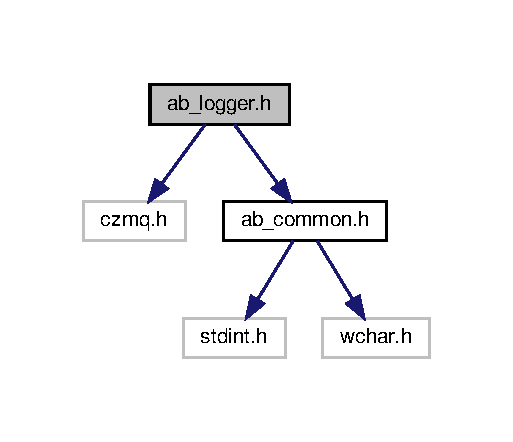
\includegraphics[width=246pt]{d3/d74/ab__logger_8h__incl}
\end{center}
\end{figure}
\doxysubsection*{Macros}
\begin{DoxyCompactItemize}
\item 
\#define \mbox{\hyperlink{ab__logger_8h_a1c3af1ceb74203276ce7ca7ec60b6e63}{abl\+\_\+trace}}(Logger,  Fmt, ...)~\mbox{\hyperlink{ab__logger_8h_a7d0be7575c2768d56ad5bdc391d3d769}{abl\+\_\+log}}(Logger, L\+O\+G\+\_\+\+T\+R\+A\+CE, \+\_\+\+\_\+\+F\+I\+L\+E\+\_\+\+\_\+, \+\_\+\+\_\+\+L\+I\+N\+E\+\_\+\+\_\+, Fmt, \+\_\+\+\_\+\+V\+A\+\_\+\+A\+R\+G\+S\+\_\+\+\_\+)
\item 
\#define \mbox{\hyperlink{ab__logger_8h_af0d95724956482b6abce967bec5bca6d}{abl\+\_\+debug}}(Logger,  Fmt, ...)~\mbox{\hyperlink{ab__logger_8h_a7d0be7575c2768d56ad5bdc391d3d769}{abl\+\_\+log}}(Logger, L\+O\+G\+\_\+\+D\+E\+B\+UG, \+\_\+\+\_\+\+F\+I\+L\+E\+\_\+\+\_\+, \+\_\+\+\_\+\+L\+I\+N\+E\+\_\+\+\_\+, Fmt, \+\_\+\+\_\+\+V\+A\+\_\+\+A\+R\+G\+S\+\_\+\+\_\+)
\item 
\#define \mbox{\hyperlink{ab__logger_8h_a0e01c4cfce56ca553e16e2f85bb9f0fe}{abl\+\_\+info}}(Logger,  Fmt, ...)~\mbox{\hyperlink{ab__logger_8h_a7d0be7575c2768d56ad5bdc391d3d769}{abl\+\_\+log}}(Logger, L\+O\+G\+\_\+\+I\+N\+FO,  \+\_\+\+\_\+\+F\+I\+L\+E\+\_\+\+\_\+, \+\_\+\+\_\+\+L\+I\+N\+E\+\_\+\+\_\+, Fmt, \+\_\+\+\_\+\+V\+A\+\_\+\+A\+R\+G\+S\+\_\+\+\_\+)
\item 
\#define \mbox{\hyperlink{ab__logger_8h_ace87fcfe98d7bb16ff20b09002b0f41b}{abl\+\_\+warn}}(Logger,  Fmt, ...)~\mbox{\hyperlink{ab__logger_8h_a7d0be7575c2768d56ad5bdc391d3d769}{abl\+\_\+log}}(Logger, L\+O\+G\+\_\+\+W\+A\+RN,  \+\_\+\+\_\+\+F\+I\+L\+E\+\_\+\+\_\+, \+\_\+\+\_\+\+L\+I\+N\+E\+\_\+\+\_\+, Fmt, \+\_\+\+\_\+\+V\+A\+\_\+\+A\+R\+G\+S\+\_\+\+\_\+)
\item 
\#define \mbox{\hyperlink{ab__logger_8h_a9701d37f9ea32885eb4435456b54380c}{abl\+\_\+error}}(Logger,  Fmt, ...)~\mbox{\hyperlink{ab__logger_8h_a7d0be7575c2768d56ad5bdc391d3d769}{abl\+\_\+log}}(Logger, L\+O\+G\+\_\+\+E\+R\+R\+OR, \+\_\+\+\_\+\+F\+I\+L\+E\+\_\+\+\_\+, \+\_\+\+\_\+\+L\+I\+N\+E\+\_\+\+\_\+, Fmt, \+\_\+\+\_\+\+V\+A\+\_\+\+A\+R\+G\+S\+\_\+\+\_\+)
\item 
\#define \mbox{\hyperlink{ab__logger_8h_a56cde45c39126f008262c3d94e03e9b8}{abl\+\_\+fatal}}(Logger,  Fmt, ...)~\mbox{\hyperlink{ab__logger_8h_a7d0be7575c2768d56ad5bdc391d3d769}{abl\+\_\+log}}(Logger, L\+O\+G\+\_\+\+F\+A\+T\+AL, \+\_\+\+\_\+\+F\+I\+L\+E\+\_\+\+\_\+, \+\_\+\+\_\+\+L\+I\+N\+E\+\_\+\+\_\+, Fmt, \+\_\+\+\_\+\+V\+A\+\_\+\+A\+R\+G\+S\+\_\+\+\_\+)
\end{DoxyCompactItemize}
\doxysubsection*{Enumerations}
\begin{DoxyCompactItemize}
\item 
enum \mbox{\hyperlink{ab__logger_8h_ad09c15c023f4bd204786f7c031c45787}{abl\+\_\+log\+\_\+level}} \{ \newline
\mbox{\hyperlink{ab__logger_8h_ad09c15c023f4bd204786f7c031c45787a7fccde42da961232bd100be86f2c32b1}{A\+B\+L\+\_\+\+T\+R\+A\+CE}}, 
\mbox{\hyperlink{ab__logger_8h_ad09c15c023f4bd204786f7c031c45787a4a4d2ab22d6f6be96611dfc75021117e}{A\+B\+L\+\_\+\+D\+E\+B\+UG}}, 
\mbox{\hyperlink{ab__logger_8h_ad09c15c023f4bd204786f7c031c45787a72e995c24ee1e50bfa27759c4c2c0bee}{A\+B\+L\+\_\+\+I\+N\+FO}}, 
\mbox{\hyperlink{ab__logger_8h_ad09c15c023f4bd204786f7c031c45787af4a847c0c5d6fe01ec92ab29b2d21144}{A\+B\+L\+\_\+\+W\+A\+RN}}, 
\newline
\mbox{\hyperlink{ab__logger_8h_ad09c15c023f4bd204786f7c031c45787a11c5fd338567ea5a3cdff6dfec3b7b5f}{A\+B\+L\+\_\+\+E\+R\+R\+OR}}, 
\mbox{\hyperlink{ab__logger_8h_ad09c15c023f4bd204786f7c031c45787a3c083097aaf5d4784c9513b0eba01e75}{A\+B\+L\+\_\+\+F\+A\+T\+AL}}
 \}
\end{DoxyCompactItemize}
\doxysubsection*{Functions}
\begin{DoxyCompactItemize}
\item 
void \mbox{\hyperlink{ab__logger_8h_adc94b6d140adcd78c7f0bb2fce524667}{abl\+\_\+start\+\_\+server}} (ab\+\_\+log $\ast$Logger, \mbox{\hyperlink{ab__common_8h_ae9b1af5c037e57a98884758875d3a7c4}{s32}} Port)
\item 
void \mbox{\hyperlink{ab__logger_8h_adce1f3ea2b2bd6eea7e33b63fd8c0499}{abl\+\_\+set\+\_\+fp}} (ab\+\_\+log $\ast$Logger, F\+I\+LE $\ast$fp)
\item 
void \mbox{\hyperlink{ab__logger_8h_ad9700e7478bc6850a033e6c1cc6eeaa1}{abl\+\_\+set\+\_\+level}} (ab\+\_\+log $\ast$Logger, \mbox{\hyperlink{ab__logger_8h_ad09c15c023f4bd204786f7c031c45787}{abl\+\_\+log\+\_\+level}} Level)
\item 
void \mbox{\hyperlink{ab__logger_8h_af26d8d70a5083e1d9c994c3e3f0b5622}{abl\+\_\+set\+\_\+quiet}} (ab\+\_\+log $\ast$Logger, \mbox{\hyperlink{ab__common_8h_a70e369648385b50f2d0588e8e8745275}{b8}} is\+Quiet)
\item 
void \mbox{\hyperlink{ab__logger_8h_a830f7af6399163b2ac8c6443042f97c7}{abl\+\_\+stop\+\_\+server}} (ab\+\_\+log $\ast$Logger)
\item 
void \mbox{\hyperlink{ab__logger_8h_a7d0be7575c2768d56ad5bdc391d3d769}{abl\+\_\+log}} (ab\+\_\+log $\ast$Logger, \mbox{\hyperlink{ab__logger_8h_ad09c15c023f4bd204786f7c031c45787}{abl\+\_\+log\+\_\+level}} Level, const char $\ast$File, \mbox{\hyperlink{ab__common_8h_ae9b1af5c037e57a98884758875d3a7c4}{s32}} Line, const char $\ast$Fmt,...)
\end{DoxyCompactItemize}


\doxysubsection{Macro Definition Documentation}
\mbox{\Hypertarget{ab__logger_8h_af0d95724956482b6abce967bec5bca6d}\label{ab__logger_8h_af0d95724956482b6abce967bec5bca6d}} 
\index{ab\_logger.h@{ab\_logger.h}!abl\_debug@{abl\_debug}}
\index{abl\_debug@{abl\_debug}!ab\_logger.h@{ab\_logger.h}}
\doxysubsubsection{\texorpdfstring{abl\_debug}{abl\_debug}}
{\footnotesize\ttfamily \#define abl\+\_\+debug(\begin{DoxyParamCaption}\item[{}]{Logger,  }\item[{}]{Fmt,  }\item[{}]{... }\end{DoxyParamCaption})~\mbox{\hyperlink{ab__logger_8h_a7d0be7575c2768d56ad5bdc391d3d769}{abl\+\_\+log}}(Logger, L\+O\+G\+\_\+\+D\+E\+B\+UG, \+\_\+\+\_\+\+F\+I\+L\+E\+\_\+\+\_\+, \+\_\+\+\_\+\+L\+I\+N\+E\+\_\+\+\_\+, Fmt, \+\_\+\+\_\+\+V\+A\+\_\+\+A\+R\+G\+S\+\_\+\+\_\+)}

\mbox{\Hypertarget{ab__logger_8h_a9701d37f9ea32885eb4435456b54380c}\label{ab__logger_8h_a9701d37f9ea32885eb4435456b54380c}} 
\index{ab\_logger.h@{ab\_logger.h}!abl\_error@{abl\_error}}
\index{abl\_error@{abl\_error}!ab\_logger.h@{ab\_logger.h}}
\doxysubsubsection{\texorpdfstring{abl\_error}{abl\_error}}
{\footnotesize\ttfamily \#define abl\+\_\+error(\begin{DoxyParamCaption}\item[{}]{Logger,  }\item[{}]{Fmt,  }\item[{}]{... }\end{DoxyParamCaption})~\mbox{\hyperlink{ab__logger_8h_a7d0be7575c2768d56ad5bdc391d3d769}{abl\+\_\+log}}(Logger, L\+O\+G\+\_\+\+E\+R\+R\+OR, \+\_\+\+\_\+\+F\+I\+L\+E\+\_\+\+\_\+, \+\_\+\+\_\+\+L\+I\+N\+E\+\_\+\+\_\+, Fmt, \+\_\+\+\_\+\+V\+A\+\_\+\+A\+R\+G\+S\+\_\+\+\_\+)}

\mbox{\Hypertarget{ab__logger_8h_a56cde45c39126f008262c3d94e03e9b8}\label{ab__logger_8h_a56cde45c39126f008262c3d94e03e9b8}} 
\index{ab\_logger.h@{ab\_logger.h}!abl\_fatal@{abl\_fatal}}
\index{abl\_fatal@{abl\_fatal}!ab\_logger.h@{ab\_logger.h}}
\doxysubsubsection{\texorpdfstring{abl\_fatal}{abl\_fatal}}
{\footnotesize\ttfamily \#define abl\+\_\+fatal(\begin{DoxyParamCaption}\item[{}]{Logger,  }\item[{}]{Fmt,  }\item[{}]{... }\end{DoxyParamCaption})~\mbox{\hyperlink{ab__logger_8h_a7d0be7575c2768d56ad5bdc391d3d769}{abl\+\_\+log}}(Logger, L\+O\+G\+\_\+\+F\+A\+T\+AL, \+\_\+\+\_\+\+F\+I\+L\+E\+\_\+\+\_\+, \+\_\+\+\_\+\+L\+I\+N\+E\+\_\+\+\_\+, Fmt, \+\_\+\+\_\+\+V\+A\+\_\+\+A\+R\+G\+S\+\_\+\+\_\+)}

\mbox{\Hypertarget{ab__logger_8h_a0e01c4cfce56ca553e16e2f85bb9f0fe}\label{ab__logger_8h_a0e01c4cfce56ca553e16e2f85bb9f0fe}} 
\index{ab\_logger.h@{ab\_logger.h}!abl\_info@{abl\_info}}
\index{abl\_info@{abl\_info}!ab\_logger.h@{ab\_logger.h}}
\doxysubsubsection{\texorpdfstring{abl\_info}{abl\_info}}
{\footnotesize\ttfamily \#define abl\+\_\+info(\begin{DoxyParamCaption}\item[{}]{Logger,  }\item[{}]{Fmt,  }\item[{}]{... }\end{DoxyParamCaption})~\mbox{\hyperlink{ab__logger_8h_a7d0be7575c2768d56ad5bdc391d3d769}{abl\+\_\+log}}(Logger, L\+O\+G\+\_\+\+I\+N\+FO,  \+\_\+\+\_\+\+F\+I\+L\+E\+\_\+\+\_\+, \+\_\+\+\_\+\+L\+I\+N\+E\+\_\+\+\_\+, Fmt, \+\_\+\+\_\+\+V\+A\+\_\+\+A\+R\+G\+S\+\_\+\+\_\+)}

\mbox{\Hypertarget{ab__logger_8h_a1c3af1ceb74203276ce7ca7ec60b6e63}\label{ab__logger_8h_a1c3af1ceb74203276ce7ca7ec60b6e63}} 
\index{ab\_logger.h@{ab\_logger.h}!abl\_trace@{abl\_trace}}
\index{abl\_trace@{abl\_trace}!ab\_logger.h@{ab\_logger.h}}
\doxysubsubsection{\texorpdfstring{abl\_trace}{abl\_trace}}
{\footnotesize\ttfamily \#define abl\+\_\+trace(\begin{DoxyParamCaption}\item[{}]{Logger,  }\item[{}]{Fmt,  }\item[{}]{... }\end{DoxyParamCaption})~\mbox{\hyperlink{ab__logger_8h_a7d0be7575c2768d56ad5bdc391d3d769}{abl\+\_\+log}}(Logger, L\+O\+G\+\_\+\+T\+R\+A\+CE, \+\_\+\+\_\+\+F\+I\+L\+E\+\_\+\+\_\+, \+\_\+\+\_\+\+L\+I\+N\+E\+\_\+\+\_\+, Fmt, \+\_\+\+\_\+\+V\+A\+\_\+\+A\+R\+G\+S\+\_\+\+\_\+)}

If multi-\/threaded, must declare a logger for use. \mbox{\Hypertarget{ab__logger_8h_ace87fcfe98d7bb16ff20b09002b0f41b}\label{ab__logger_8h_ace87fcfe98d7bb16ff20b09002b0f41b}} 
\index{ab\_logger.h@{ab\_logger.h}!abl\_warn@{abl\_warn}}
\index{abl\_warn@{abl\_warn}!ab\_logger.h@{ab\_logger.h}}
\doxysubsubsection{\texorpdfstring{abl\_warn}{abl\_warn}}
{\footnotesize\ttfamily \#define abl\+\_\+warn(\begin{DoxyParamCaption}\item[{}]{Logger,  }\item[{}]{Fmt,  }\item[{}]{... }\end{DoxyParamCaption})~\mbox{\hyperlink{ab__logger_8h_a7d0be7575c2768d56ad5bdc391d3d769}{abl\+\_\+log}}(Logger, L\+O\+G\+\_\+\+W\+A\+RN,  \+\_\+\+\_\+\+F\+I\+L\+E\+\_\+\+\_\+, \+\_\+\+\_\+\+L\+I\+N\+E\+\_\+\+\_\+, Fmt, \+\_\+\+\_\+\+V\+A\+\_\+\+A\+R\+G\+S\+\_\+\+\_\+)}



\doxysubsection{Enumeration Type Documentation}
\mbox{\Hypertarget{ab__logger_8h_ad09c15c023f4bd204786f7c031c45787}\label{ab__logger_8h_ad09c15c023f4bd204786f7c031c45787}} 
\index{ab\_logger.h@{ab\_logger.h}!abl\_log\_level@{abl\_log\_level}}
\index{abl\_log\_level@{abl\_log\_level}!ab\_logger.h@{ab\_logger.h}}
\doxysubsubsection{\texorpdfstring{abl\_log\_level}{abl\_log\_level}}
{\footnotesize\ttfamily enum \mbox{\hyperlink{ab__logger_8h_ad09c15c023f4bd204786f7c031c45787}{abl\+\_\+log\+\_\+level}}}

Logger. Version\+: 1.\+0 Network logger using czmq. Will log to S\+T\+D\+E\+RR, a file and/or to a czmq network, depending on setup. S\+T\+D\+E\+RR logging not garunteed to be threadsafe, don\textquotesingle{}t do it. Logging multiple threads to the same file not garunteed to be threadsafe. C\+Z\+MQ logging is threadsafe subject to the restrictions of C\+Z\+MQ.

Basically, use a different ab\+\_\+log for each thread and you should be ok.

This is a single-\/file-\/library. You may include the file anywhere in your source. Only once in your code, define the following\+:


\begin{DoxyCode}{0}
\DoxyCodeLine{\textcolor{preprocessor}{\#define AB\_LOGGER\_SRC}}
\DoxyCodeLine{\textcolor{preprocessor}{\#include "{}ab\_logger.h"{}}}
\end{DoxyCode}


This will include the source.

There\textquotesingle{}s a single-\/thread use that uses a global logger. Define the following\+: 
\begin{DoxyCode}{0}
\DoxyCodeLine{\textcolor{preprocessor}{\#define AB\_LOGGER\_SINGLETHREAD}}
\end{DoxyCode}


To use color on S\+T\+D\+E\+RR\+: 
\begin{DoxyCode}{0}
\DoxyCodeLine{\textcolor{preprocessor}{\#define AB\_LOGGER\_USE\_COLOR}}
\end{DoxyCode}


Available levels\+: A\+B\+L\+\_\+\+T\+R\+A\+CE, A\+B\+L\+\_\+\+D\+E\+B\+UG, A\+B\+L\+\_\+\+I\+N\+FO, A\+B\+L\+\_\+\+W\+A\+RN, A\+B\+L\+\_\+\+E\+R\+R\+OR, A\+B\+L\+\_\+\+F\+A\+T\+AL

example usage\+: abl\+\_\+log Logger = \{\}; abl\+\_\+set\+\_\+level(\&\+Logger, A\+B\+L\+\_\+\+I\+N\+F\+O); abl\+\_\+start\+\_\+server(\&\+Logger, 555); abl\+\_\+info(\&Logger, \char`\"{}\+Some log\char`\"{}); abl\+\_\+info(\&Logger, \char`\"{}\+More Info, \%d\char`\"{}, errno); abl\+\_\+stop\+\_\+server(\&\+Logger); \begin{DoxyEnumFields}{Enumerator}
\raisebox{\heightof{T}}[0pt][0pt]{\index{ABL\_TRACE@{ABL\_TRACE}!ab\_logger.h@{ab\_logger.h}}\index{ab\_logger.h@{ab\_logger.h}!ABL\_TRACE@{ABL\_TRACE}}}\mbox{\Hypertarget{ab__logger_8h_ad09c15c023f4bd204786f7c031c45787a7fccde42da961232bd100be86f2c32b1}\label{ab__logger_8h_ad09c15c023f4bd204786f7c031c45787a7fccde42da961232bd100be86f2c32b1}} 
A\+B\+L\+\_\+\+T\+R\+A\+CE&\\
\hline

\raisebox{\heightof{T}}[0pt][0pt]{\index{ABL\_DEBUG@{ABL\_DEBUG}!ab\_logger.h@{ab\_logger.h}}\index{ab\_logger.h@{ab\_logger.h}!ABL\_DEBUG@{ABL\_DEBUG}}}\mbox{\Hypertarget{ab__logger_8h_ad09c15c023f4bd204786f7c031c45787a4a4d2ab22d6f6be96611dfc75021117e}\label{ab__logger_8h_ad09c15c023f4bd204786f7c031c45787a4a4d2ab22d6f6be96611dfc75021117e}} 
A\+B\+L\+\_\+\+D\+E\+B\+UG&\\
\hline

\raisebox{\heightof{T}}[0pt][0pt]{\index{ABL\_INFO@{ABL\_INFO}!ab\_logger.h@{ab\_logger.h}}\index{ab\_logger.h@{ab\_logger.h}!ABL\_INFO@{ABL\_INFO}}}\mbox{\Hypertarget{ab__logger_8h_ad09c15c023f4bd204786f7c031c45787a72e995c24ee1e50bfa27759c4c2c0bee}\label{ab__logger_8h_ad09c15c023f4bd204786f7c031c45787a72e995c24ee1e50bfa27759c4c2c0bee}} 
A\+B\+L\+\_\+\+I\+N\+FO&\\
\hline

\raisebox{\heightof{T}}[0pt][0pt]{\index{ABL\_WARN@{ABL\_WARN}!ab\_logger.h@{ab\_logger.h}}\index{ab\_logger.h@{ab\_logger.h}!ABL\_WARN@{ABL\_WARN}}}\mbox{\Hypertarget{ab__logger_8h_ad09c15c023f4bd204786f7c031c45787af4a847c0c5d6fe01ec92ab29b2d21144}\label{ab__logger_8h_ad09c15c023f4bd204786f7c031c45787af4a847c0c5d6fe01ec92ab29b2d21144}} 
A\+B\+L\+\_\+\+W\+A\+RN&\\
\hline

\raisebox{\heightof{T}}[0pt][0pt]{\index{ABL\_ERROR@{ABL\_ERROR}!ab\_logger.h@{ab\_logger.h}}\index{ab\_logger.h@{ab\_logger.h}!ABL\_ERROR@{ABL\_ERROR}}}\mbox{\Hypertarget{ab__logger_8h_ad09c15c023f4bd204786f7c031c45787a11c5fd338567ea5a3cdff6dfec3b7b5f}\label{ab__logger_8h_ad09c15c023f4bd204786f7c031c45787a11c5fd338567ea5a3cdff6dfec3b7b5f}} 
A\+B\+L\+\_\+\+E\+R\+R\+OR&\\
\hline

\raisebox{\heightof{T}}[0pt][0pt]{\index{ABL\_FATAL@{ABL\_FATAL}!ab\_logger.h@{ab\_logger.h}}\index{ab\_logger.h@{ab\_logger.h}!ABL\_FATAL@{ABL\_FATAL}}}\mbox{\Hypertarget{ab__logger_8h_ad09c15c023f4bd204786f7c031c45787a3c083097aaf5d4784c9513b0eba01e75}\label{ab__logger_8h_ad09c15c023f4bd204786f7c031c45787a3c083097aaf5d4784c9513b0eba01e75}} 
A\+B\+L\+\_\+\+F\+A\+T\+AL&\\
\hline

\end{DoxyEnumFields}


\doxysubsection{Function Documentation}
\mbox{\Hypertarget{ab__logger_8h_a7d0be7575c2768d56ad5bdc391d3d769}\label{ab__logger_8h_a7d0be7575c2768d56ad5bdc391d3d769}} 
\index{ab\_logger.h@{ab\_logger.h}!abl\_log@{abl\_log}}
\index{abl\_log@{abl\_log}!ab\_logger.h@{ab\_logger.h}}
\doxysubsubsection{\texorpdfstring{abl\_log()}{abl\_log()}}
{\footnotesize\ttfamily void abl\+\_\+log (\begin{DoxyParamCaption}\item[{ab\+\_\+log $\ast$}]{Logger,  }\item[{\mbox{\hyperlink{ab__logger_8h_ad09c15c023f4bd204786f7c031c45787}{abl\+\_\+log\+\_\+level}}}]{Level,  }\item[{const char $\ast$}]{File,  }\item[{\mbox{\hyperlink{ab__common_8h_ae9b1af5c037e57a98884758875d3a7c4}{s32}}}]{Line,  }\item[{const char $\ast$}]{Fmt,  }\item[{}]{... }\end{DoxyParamCaption})}

\mbox{\Hypertarget{ab__logger_8h_adce1f3ea2b2bd6eea7e33b63fd8c0499}\label{ab__logger_8h_adce1f3ea2b2bd6eea7e33b63fd8c0499}} 
\index{ab\_logger.h@{ab\_logger.h}!abl\_set\_fp@{abl\_set\_fp}}
\index{abl\_set\_fp@{abl\_set\_fp}!ab\_logger.h@{ab\_logger.h}}
\doxysubsubsection{\texorpdfstring{abl\_set\_fp()}{abl\_set\_fp()}}
{\footnotesize\ttfamily void abl\+\_\+set\+\_\+fp (\begin{DoxyParamCaption}\item[{ab\+\_\+log $\ast$}]{Logger,  }\item[{F\+I\+LE $\ast$}]{fp }\end{DoxyParamCaption})}

\mbox{\Hypertarget{ab__logger_8h_ad9700e7478bc6850a033e6c1cc6eeaa1}\label{ab__logger_8h_ad9700e7478bc6850a033e6c1cc6eeaa1}} 
\index{ab\_logger.h@{ab\_logger.h}!abl\_set\_level@{abl\_set\_level}}
\index{abl\_set\_level@{abl\_set\_level}!ab\_logger.h@{ab\_logger.h}}
\doxysubsubsection{\texorpdfstring{abl\_set\_level()}{abl\_set\_level()}}
{\footnotesize\ttfamily void abl\+\_\+set\+\_\+level (\begin{DoxyParamCaption}\item[{ab\+\_\+log $\ast$}]{Logger,  }\item[{\mbox{\hyperlink{ab__logger_8h_ad09c15c023f4bd204786f7c031c45787}{abl\+\_\+log\+\_\+level}}}]{Level }\end{DoxyParamCaption})}

\mbox{\Hypertarget{ab__logger_8h_af26d8d70a5083e1d9c994c3e3f0b5622}\label{ab__logger_8h_af26d8d70a5083e1d9c994c3e3f0b5622}} 
\index{ab\_logger.h@{ab\_logger.h}!abl\_set\_quiet@{abl\_set\_quiet}}
\index{abl\_set\_quiet@{abl\_set\_quiet}!ab\_logger.h@{ab\_logger.h}}
\doxysubsubsection{\texorpdfstring{abl\_set\_quiet()}{abl\_set\_quiet()}}
{\footnotesize\ttfamily void abl\+\_\+set\+\_\+quiet (\begin{DoxyParamCaption}\item[{ab\+\_\+log $\ast$}]{Logger,  }\item[{\mbox{\hyperlink{ab__common_8h_a70e369648385b50f2d0588e8e8745275}{b8}}}]{is\+Quiet }\end{DoxyParamCaption})}

\mbox{\Hypertarget{ab__logger_8h_adc94b6d140adcd78c7f0bb2fce524667}\label{ab__logger_8h_adc94b6d140adcd78c7f0bb2fce524667}} 
\index{ab\_logger.h@{ab\_logger.h}!abl\_start\_server@{abl\_start\_server}}
\index{abl\_start\_server@{abl\_start\_server}!ab\_logger.h@{ab\_logger.h}}
\doxysubsubsection{\texorpdfstring{abl\_start\_server()}{abl\_start\_server()}}
{\footnotesize\ttfamily void abl\+\_\+start\+\_\+server (\begin{DoxyParamCaption}\item[{ab\+\_\+log $\ast$}]{Logger,  }\item[{\mbox{\hyperlink{ab__common_8h_ae9b1af5c037e57a98884758875d3a7c4}{s32}}}]{Port }\end{DoxyParamCaption})}

\mbox{\Hypertarget{ab__logger_8h_a830f7af6399163b2ac8c6443042f97c7}\label{ab__logger_8h_a830f7af6399163b2ac8c6443042f97c7}} 
\index{ab\_logger.h@{ab\_logger.h}!abl\_stop\_server@{abl\_stop\_server}}
\index{abl\_stop\_server@{abl\_stop\_server}!ab\_logger.h@{ab\_logger.h}}
\doxysubsubsection{\texorpdfstring{abl\_stop\_server()}{abl\_stop\_server()}}
{\footnotesize\ttfamily void abl\+\_\+stop\+\_\+server (\begin{DoxyParamCaption}\item[{ab\+\_\+log $\ast$}]{Logger }\end{DoxyParamCaption})}

set is\+Quiet = true -\/$>$ true to disable logging to S\+T\+D\+E\+RR. 
\hypertarget{ab__memory_8h}{}\section{ab\+\_\+memory.\+h File Reference}
\label{ab__memory_8h}\index{ab\+\_\+memory.\+h@{ab\+\_\+memory.\+h}}
{\ttfamily \#include \char`\"{}ab\+\_\+common.\+h\char`\"{}}\newline
Include dependency graph for ab\+\_\+memory.\+h\+:\nopagebreak
\begin{figure}[H]
\begin{center}
\leavevmode
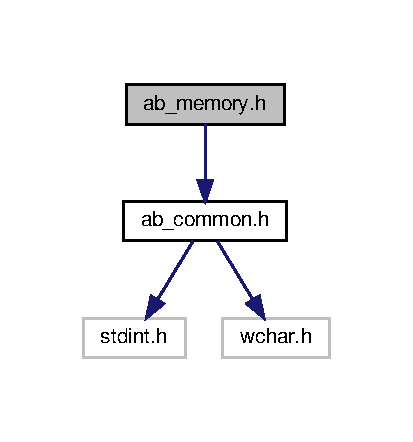
\includegraphics[width=198pt]{d7/d5f/ab__memory_8h__incl}
\end{center}
\end{figure}
This graph shows which files directly or indirectly include this file\+:\nopagebreak
\begin{figure}[H]
\begin{center}
\leavevmode
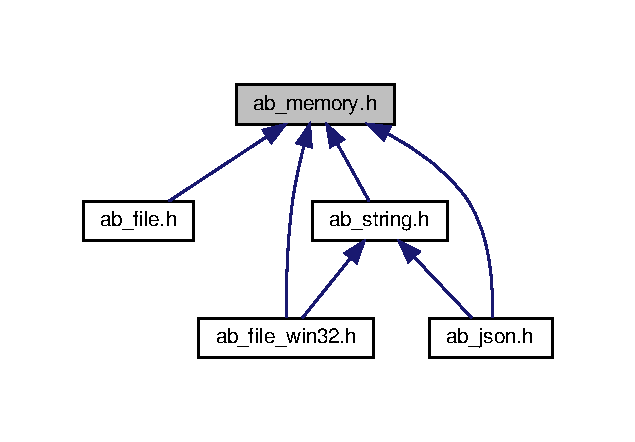
\includegraphics[width=350pt]{d4/d8c/ab__memory_8h__dep__incl}
\end{center}
\end{figure}
\subsection*{Classes}
\begin{DoxyCompactItemize}
\item 
struct \hyperlink{structmemory__arena}{memory\+\_\+arena}
\item 
struct \hyperlink{structtemporary__memory}{temporary\+\_\+memory}
\end{DoxyCompactItemize}
\subsection*{Macros}
\begin{DoxyCompactItemize}
\item 
\#define \hyperlink{ab__memory_8h_a0436d3ae4dac7362742c35ea6a146fea}{abm\+\_\+\+Push\+Struct}(Arena,  Type)~(Type$\ast$)\hyperlink{ab__memory_8h_a15270c8569eb858cdb20ee45c3bb46f7}{abm\+\_\+\+Push\+Size\+\_\+}(Arena, sizeof(Type))
\item 
\#define \hyperlink{ab__memory_8h_ab8d45b257f787efccb8a928176cc2c88}{abm\+\_\+\+Push\+Size}(Arena,  Size)~\hyperlink{ab__memory_8h_a15270c8569eb858cdb20ee45c3bb46f7}{abm\+\_\+\+Push\+Size\+\_\+}(Arena, Size)
\item 
\#define \hyperlink{ab__memory_8h_a89df166532e625eea593369a7997139d}{abm\+\_\+\+Push\+Array}(Arena,  Count,  Type)~(Type$\ast$)\hyperlink{ab__memory_8h_a15270c8569eb858cdb20ee45c3bb46f7}{abm\+\_\+\+Push\+Size\+\_\+}(Arena, (Count)$\ast$sizeof(Type))
\end{DoxyCompactItemize}
\subsection*{Functions}
\begin{DoxyCompactItemize}
\item 
void $\ast$ \hyperlink{ab__memory_8h_a20bffb2c2335745a56275b6094b6dcad}{abm\+\_\+\+Allocate\+Os\+Memory} (void $\ast$Address, size\+\_\+t Size)
\item 
void \hyperlink{ab__memory_8h_ad393d506412ba1d8d6fe25e8e16253b4}{abm\+\_\+\+Deallocate\+Os\+Memory} (void $\ast$Address, size\+\_\+t Size)
\item 
void $\ast$ \hyperlink{ab__memory_8h_a15270c8569eb858cdb20ee45c3bb46f7}{abm\+\_\+\+Push\+Size\+\_\+} (\hyperlink{structmemory__arena}{memory\+\_\+arena} $\ast$Memory, size\+\_\+t Size, \hyperlink{ab__common_8h_a70e369648385b50f2d0588e8e8745275}{b8} Clear\+Memory=true)
\item 
\hyperlink{structmemory__arena}{memory\+\_\+arena} \hyperlink{ab__memory_8h_a5f2fa70a405694492db91b26ed884207}{abm\+\_\+\+Init\+Memory} (void $\ast$Start, size\+\_\+t Size)
\item 
void \hyperlink{ab__memory_8h_a8ca432174a01c886b3c834cbb140c5ab}{abm\+\_\+\+Reset\+Memory} (\hyperlink{structmemory__arena}{memory\+\_\+arena} $\ast$Memory)
\item 
size\+\_\+t \hyperlink{ab__memory_8h_a9061bfb19b910033ab211832bc593fed}{abm\+\_\+\+Get\+Memory\+Left} (\hyperlink{structmemory__arena}{memory\+\_\+arena} $\ast$Memory)
\item 
\hyperlink{structtemporary__memory}{temporary\+\_\+memory} \hyperlink{ab__memory_8h_a77b6adde3ba40f7f3777bcc01c396ccd}{abm\+\_\+\+Begin\+Temporary\+Memory} (\hyperlink{structmemory__arena}{memory\+\_\+arena} $\ast$Memory)
\item 
void \hyperlink{ab__memory_8h_a8dbf22e067d85b9ad8422126755d23df}{abm\+\_\+\+End\+Temporary\+Memory} (\hyperlink{structtemporary__memory}{temporary\+\_\+memory} Temp\+Mem)
\item 
\hyperlink{structmemory__arena}{memory\+\_\+arena} \hyperlink{ab__memory_8h_a1b0ab8d04e6309ae31b1b2f8282dc085}{abm\+\_\+\+Create\+Sub\+Arena} (\hyperlink{structmemory__arena}{memory\+\_\+arena} $\ast$Memory, size\+\_\+t Size)
\end{DoxyCompactItemize}


\subsection{Macro Definition Documentation}
\mbox{\Hypertarget{ab__memory_8h_a89df166532e625eea593369a7997139d}\label{ab__memory_8h_a89df166532e625eea593369a7997139d}} 
\index{ab\+\_\+memory.\+h@{ab\+\_\+memory.\+h}!abm\+\_\+\+Push\+Array@{abm\+\_\+\+Push\+Array}}
\index{abm\+\_\+\+Push\+Array@{abm\+\_\+\+Push\+Array}!ab\+\_\+memory.\+h@{ab\+\_\+memory.\+h}}
\subsubsection{\texorpdfstring{abm\+\_\+\+Push\+Array}{abm\_PushArray}}
{\footnotesize\ttfamily \#define abm\+\_\+\+Push\+Array(\begin{DoxyParamCaption}\item[{}]{Arena,  }\item[{}]{Count,  }\item[{}]{Type }\end{DoxyParamCaption})~(Type$\ast$)\hyperlink{ab__memory_8h_a15270c8569eb858cdb20ee45c3bb46f7}{abm\+\_\+\+Push\+Size\+\_\+}(Arena, (Count)$\ast$sizeof(Type))}

\mbox{\Hypertarget{ab__memory_8h_ab8d45b257f787efccb8a928176cc2c88}\label{ab__memory_8h_ab8d45b257f787efccb8a928176cc2c88}} 
\index{ab\+\_\+memory.\+h@{ab\+\_\+memory.\+h}!abm\+\_\+\+Push\+Size@{abm\+\_\+\+Push\+Size}}
\index{abm\+\_\+\+Push\+Size@{abm\+\_\+\+Push\+Size}!ab\+\_\+memory.\+h@{ab\+\_\+memory.\+h}}
\subsubsection{\texorpdfstring{abm\+\_\+\+Push\+Size}{abm\_PushSize}}
{\footnotesize\ttfamily \#define abm\+\_\+\+Push\+Size(\begin{DoxyParamCaption}\item[{}]{Arena,  }\item[{}]{Size }\end{DoxyParamCaption})~\hyperlink{ab__memory_8h_a15270c8569eb858cdb20ee45c3bb46f7}{abm\+\_\+\+Push\+Size\+\_\+}(Arena, Size)}

\mbox{\Hypertarget{ab__memory_8h_a0436d3ae4dac7362742c35ea6a146fea}\label{ab__memory_8h_a0436d3ae4dac7362742c35ea6a146fea}} 
\index{ab\+\_\+memory.\+h@{ab\+\_\+memory.\+h}!abm\+\_\+\+Push\+Struct@{abm\+\_\+\+Push\+Struct}}
\index{abm\+\_\+\+Push\+Struct@{abm\+\_\+\+Push\+Struct}!ab\+\_\+memory.\+h@{ab\+\_\+memory.\+h}}
\subsubsection{\texorpdfstring{abm\+\_\+\+Push\+Struct}{abm\_PushStruct}}
{\footnotesize\ttfamily \#define abm\+\_\+\+Push\+Struct(\begin{DoxyParamCaption}\item[{}]{Arena,  }\item[{}]{Type }\end{DoxyParamCaption})~(Type$\ast$)\hyperlink{ab__memory_8h_a15270c8569eb858cdb20ee45c3bb46f7}{abm\+\_\+\+Push\+Size\+\_\+}(Arena, sizeof(Type))}



\subsection{Function Documentation}
\mbox{\Hypertarget{ab__memory_8h_a20bffb2c2335745a56275b6094b6dcad}\label{ab__memory_8h_a20bffb2c2335745a56275b6094b6dcad}} 
\index{ab\+\_\+memory.\+h@{ab\+\_\+memory.\+h}!abm\+\_\+\+Allocate\+Os\+Memory@{abm\+\_\+\+Allocate\+Os\+Memory}}
\index{abm\+\_\+\+Allocate\+Os\+Memory@{abm\+\_\+\+Allocate\+Os\+Memory}!ab\+\_\+memory.\+h@{ab\+\_\+memory.\+h}}
\subsubsection{\texorpdfstring{abm\+\_\+\+Allocate\+Os\+Memory()}{abm\_AllocateOsMemory()}}
{\footnotesize\ttfamily void$\ast$ abm\+\_\+\+Allocate\+Os\+Memory (\begin{DoxyParamCaption}\item[{void $\ast$}]{Address,  }\item[{size\+\_\+t}]{Size }\end{DoxyParamCaption})}

\mbox{\Hypertarget{ab__memory_8h_a77b6adde3ba40f7f3777bcc01c396ccd}\label{ab__memory_8h_a77b6adde3ba40f7f3777bcc01c396ccd}} 
\index{ab\+\_\+memory.\+h@{ab\+\_\+memory.\+h}!abm\+\_\+\+Begin\+Temporary\+Memory@{abm\+\_\+\+Begin\+Temporary\+Memory}}
\index{abm\+\_\+\+Begin\+Temporary\+Memory@{abm\+\_\+\+Begin\+Temporary\+Memory}!ab\+\_\+memory.\+h@{ab\+\_\+memory.\+h}}
\subsubsection{\texorpdfstring{abm\+\_\+\+Begin\+Temporary\+Memory()}{abm\_BeginTemporaryMemory()}}
{\footnotesize\ttfamily \hyperlink{structtemporary__memory}{temporary\+\_\+memory} abm\+\_\+\+Begin\+Temporary\+Memory (\begin{DoxyParamCaption}\item[{\hyperlink{structmemory__arena}{memory\+\_\+arena} $\ast$}]{Memory }\end{DoxyParamCaption})}

\mbox{\Hypertarget{ab__memory_8h_a1b0ab8d04e6309ae31b1b2f8282dc085}\label{ab__memory_8h_a1b0ab8d04e6309ae31b1b2f8282dc085}} 
\index{ab\+\_\+memory.\+h@{ab\+\_\+memory.\+h}!abm\+\_\+\+Create\+Sub\+Arena@{abm\+\_\+\+Create\+Sub\+Arena}}
\index{abm\+\_\+\+Create\+Sub\+Arena@{abm\+\_\+\+Create\+Sub\+Arena}!ab\+\_\+memory.\+h@{ab\+\_\+memory.\+h}}
\subsubsection{\texorpdfstring{abm\+\_\+\+Create\+Sub\+Arena()}{abm\_CreateSubArena()}}
{\footnotesize\ttfamily \hyperlink{structmemory__arena}{memory\+\_\+arena} abm\+\_\+\+Create\+Sub\+Arena (\begin{DoxyParamCaption}\item[{\hyperlink{structmemory__arena}{memory\+\_\+arena} $\ast$}]{Memory,  }\item[{size\+\_\+t}]{Size }\end{DoxyParamCaption})}

\mbox{\Hypertarget{ab__memory_8h_ad393d506412ba1d8d6fe25e8e16253b4}\label{ab__memory_8h_ad393d506412ba1d8d6fe25e8e16253b4}} 
\index{ab\+\_\+memory.\+h@{ab\+\_\+memory.\+h}!abm\+\_\+\+Deallocate\+Os\+Memory@{abm\+\_\+\+Deallocate\+Os\+Memory}}
\index{abm\+\_\+\+Deallocate\+Os\+Memory@{abm\+\_\+\+Deallocate\+Os\+Memory}!ab\+\_\+memory.\+h@{ab\+\_\+memory.\+h}}
\subsubsection{\texorpdfstring{abm\+\_\+\+Deallocate\+Os\+Memory()}{abm\_DeallocateOsMemory()}}
{\footnotesize\ttfamily void abm\+\_\+\+Deallocate\+Os\+Memory (\begin{DoxyParamCaption}\item[{void $\ast$}]{Address,  }\item[{size\+\_\+t}]{Size }\end{DoxyParamCaption})}

\mbox{\Hypertarget{ab__memory_8h_a8dbf22e067d85b9ad8422126755d23df}\label{ab__memory_8h_a8dbf22e067d85b9ad8422126755d23df}} 
\index{ab\+\_\+memory.\+h@{ab\+\_\+memory.\+h}!abm\+\_\+\+End\+Temporary\+Memory@{abm\+\_\+\+End\+Temporary\+Memory}}
\index{abm\+\_\+\+End\+Temporary\+Memory@{abm\+\_\+\+End\+Temporary\+Memory}!ab\+\_\+memory.\+h@{ab\+\_\+memory.\+h}}
\subsubsection{\texorpdfstring{abm\+\_\+\+End\+Temporary\+Memory()}{abm\_EndTemporaryMemory()}}
{\footnotesize\ttfamily void abm\+\_\+\+End\+Temporary\+Memory (\begin{DoxyParamCaption}\item[{\hyperlink{structtemporary__memory}{temporary\+\_\+memory}}]{Temp\+Mem }\end{DoxyParamCaption})}

\mbox{\Hypertarget{ab__memory_8h_a9061bfb19b910033ab211832bc593fed}\label{ab__memory_8h_a9061bfb19b910033ab211832bc593fed}} 
\index{ab\+\_\+memory.\+h@{ab\+\_\+memory.\+h}!abm\+\_\+\+Get\+Memory\+Left@{abm\+\_\+\+Get\+Memory\+Left}}
\index{abm\+\_\+\+Get\+Memory\+Left@{abm\+\_\+\+Get\+Memory\+Left}!ab\+\_\+memory.\+h@{ab\+\_\+memory.\+h}}
\subsubsection{\texorpdfstring{abm\+\_\+\+Get\+Memory\+Left()}{abm\_GetMemoryLeft()}}
{\footnotesize\ttfamily size\+\_\+t abm\+\_\+\+Get\+Memory\+Left (\begin{DoxyParamCaption}\item[{\hyperlink{structmemory__arena}{memory\+\_\+arena} $\ast$}]{Memory }\end{DoxyParamCaption})\hspace{0.3cm}{\ttfamily [inline]}}

\mbox{\Hypertarget{ab__memory_8h_a5f2fa70a405694492db91b26ed884207}\label{ab__memory_8h_a5f2fa70a405694492db91b26ed884207}} 
\index{ab\+\_\+memory.\+h@{ab\+\_\+memory.\+h}!abm\+\_\+\+Init\+Memory@{abm\+\_\+\+Init\+Memory}}
\index{abm\+\_\+\+Init\+Memory@{abm\+\_\+\+Init\+Memory}!ab\+\_\+memory.\+h@{ab\+\_\+memory.\+h}}
\subsubsection{\texorpdfstring{abm\+\_\+\+Init\+Memory()}{abm\_InitMemory()}}
{\footnotesize\ttfamily \hyperlink{structmemory__arena}{memory\+\_\+arena} abm\+\_\+\+Init\+Memory (\begin{DoxyParamCaption}\item[{void $\ast$}]{Start,  }\item[{size\+\_\+t}]{Size }\end{DoxyParamCaption})}

\mbox{\Hypertarget{ab__memory_8h_a15270c8569eb858cdb20ee45c3bb46f7}\label{ab__memory_8h_a15270c8569eb858cdb20ee45c3bb46f7}} 
\index{ab\+\_\+memory.\+h@{ab\+\_\+memory.\+h}!abm\+\_\+\+Push\+Size\+\_\+@{abm\+\_\+\+Push\+Size\+\_\+}}
\index{abm\+\_\+\+Push\+Size\+\_\+@{abm\+\_\+\+Push\+Size\+\_\+}!ab\+\_\+memory.\+h@{ab\+\_\+memory.\+h}}
\subsubsection{\texorpdfstring{abm\+\_\+\+Push\+Size\+\_\+()}{abm\_PushSize\_()}}
{\footnotesize\ttfamily void$\ast$ abm\+\_\+\+Push\+Size\+\_\+ (\begin{DoxyParamCaption}\item[{\hyperlink{structmemory__arena}{memory\+\_\+arena} $\ast$}]{Memory,  }\item[{size\+\_\+t}]{Size,  }\item[{\hyperlink{ab__common_8h_a70e369648385b50f2d0588e8e8745275}{b8}}]{Clear\+Memory = {\ttfamily true} }\end{DoxyParamCaption})}

\mbox{\Hypertarget{ab__memory_8h_a8ca432174a01c886b3c834cbb140c5ab}\label{ab__memory_8h_a8ca432174a01c886b3c834cbb140c5ab}} 
\index{ab\+\_\+memory.\+h@{ab\+\_\+memory.\+h}!abm\+\_\+\+Reset\+Memory@{abm\+\_\+\+Reset\+Memory}}
\index{abm\+\_\+\+Reset\+Memory@{abm\+\_\+\+Reset\+Memory}!ab\+\_\+memory.\+h@{ab\+\_\+memory.\+h}}
\subsubsection{\texorpdfstring{abm\+\_\+\+Reset\+Memory()}{abm\_ResetMemory()}}
{\footnotesize\ttfamily void abm\+\_\+\+Reset\+Memory (\begin{DoxyParamCaption}\item[{\hyperlink{structmemory__arena}{memory\+\_\+arena} $\ast$}]{Memory }\end{DoxyParamCaption})}


\hypertarget{ab__memory__linux_8h}{}\doxysection{ab\+\_\+memory\+\_\+linux.\+h File Reference}
\label{ab__memory__linux_8h}\index{ab\_memory\_linux.h@{ab\_memory\_linux.h}}


Linux specific implementation of some memory functions.  




\doxysubsection{Detailed Description}
Linux specific implementation of some memory functions. 

\begin{DoxyAuthor}{Author}
Amos Buchanan 
\end{DoxyAuthor}
\begin{DoxyVersion}{Version}
1.\+0 
\end{DoxyVersion}
\begin{DoxyDate}{Date}
2020 
\end{DoxyDate}
\begin{DoxyCopyright}{Copyright}
\href{https://opensource.org/licenses/MIT}{\texttt{ M\+IT Public License}}
\end{DoxyCopyright}
Linux specific implementation of functions. See \mbox{\hyperlink{ab__memory_8h}{ab\+\_\+memory.\+h}} for function usage. Do not include this file directly; it\textquotesingle{}s included from \mbox{\hyperlink{ab__memory_8h}{ab\+\_\+memory.\+h}} automatically.

\doxysubsection*{M\+IT License}

\href{https://opensource.org/licenses/MIT}{\texttt{ M\+IT Public License}}

Copyright 2020 Amos Buchanan

Permission is hereby granted, free of charge, to any person obtaining a copy of this software and associated documentation files (the \char`\"{}\+Software\char`\"{}), to deal in the Software without restriction, including without limitation the rights to use, copy, modify, merge, publish, distribute, sublicense, and/or sell copies of the Software, and to permit persons to whom the Software is furnished to do so, subject to the following conditions\+:

The above copyright notice and this permission notice shall be included in all copies or substantial portions of the Software.

T\+HE S\+O\+F\+T\+W\+A\+RE IS P\+R\+O\+V\+I\+D\+ED \char`\"{}\+A\+S I\+S\char`\"{}, W\+I\+T\+H\+O\+UT W\+A\+R\+R\+A\+N\+TY OF A\+NY K\+I\+ND, E\+X\+P\+R\+E\+SS OR I\+M\+P\+L\+I\+ED, I\+N\+C\+L\+U\+D\+I\+NG B\+UT N\+OT L\+I\+M\+I\+T\+ED TO T\+HE W\+A\+R\+R\+A\+N\+T\+I\+ES OF M\+E\+R\+C\+H\+A\+N\+T\+A\+B\+I\+L\+I\+TY, F\+I\+T\+N\+E\+SS F\+OR A P\+A\+R\+T\+I\+C\+U\+L\+AR P\+U\+R\+P\+O\+SE A\+ND N\+O\+N\+I\+N\+F\+R\+I\+N\+G\+E\+M\+E\+NT. IN NO E\+V\+E\+NT S\+H\+A\+LL T\+HE A\+U\+T\+H\+O\+RS OR C\+O\+P\+Y\+R\+I\+G\+HT H\+O\+L\+D\+E\+RS BE L\+I\+A\+B\+LE F\+OR A\+NY C\+L\+A\+IM, D\+A\+M\+A\+G\+ES OR O\+T\+H\+ER L\+I\+A\+B\+I\+L\+I\+TY, W\+H\+E\+T\+H\+ER IN AN A\+C\+T\+I\+ON OF C\+O\+N\+T\+R\+A\+CT, T\+O\+RT OR O\+T\+H\+E\+R\+W\+I\+SE, A\+R\+I\+S\+I\+NG F\+R\+OM, O\+UT OF OR IN C\+O\+N\+N\+E\+C\+T\+I\+ON W\+I\+TH T\+HE S\+O\+F\+T\+W\+A\+RE OR T\+HE U\+SE OR O\+T\+H\+ER D\+E\+A\+L\+I\+N\+GS IN T\+HE S\+O\+F\+T\+W\+A\+RE. 
\hypertarget{ab__memory__win32_8h}{}\doxysection{ab\+\_\+memory\+\_\+win32.\+h File Reference}
\label{ab__memory__win32_8h}\index{ab\_memory\_win32.h@{ab\_memory\_win32.h}}


Windows specific implementation of some memory functions.  




\doxysubsection{Detailed Description}
Windows specific implementation of some memory functions. 

\begin{DoxyAuthor}{Author}
Amos Buchanan 
\end{DoxyAuthor}
\begin{DoxyVersion}{Version}
1.\+0 
\end{DoxyVersion}
\begin{DoxyDate}{Date}
2020
\end{DoxyDate}
Windows specific implementation of functions. See \mbox{\hyperlink{ab__memory_8h}{ab\+\_\+memory.\+h}} for function usage. Do not include this file directly; it\textquotesingle{}s included from \mbox{\hyperlink{ab__memory_8h}{ab\+\_\+memory.\+h}} automatically. 
\hypertarget{ab__parser_8cpp}{}\section{ab\+\_\+parser.\+cpp File Reference}
\label{ab__parser_8cpp}\index{ab\+\_\+parser.\+cpp@{ab\+\_\+parser.\+cpp}}

\hypertarget{ab__parser_8h}{}\section{ab\+\_\+parser.\+h File Reference}
\label{ab__parser_8h}\index{ab\+\_\+parser.\+h@{ab\+\_\+parser.\+h}}
{\ttfamily \#include \char`\"{}ab\+\_\+lexer.\+h\char`\"{}}\newline
Include dependency graph for ab\+\_\+parser.\+h\+:
\nopagebreak
\begin{figure}[H]
\begin{center}
\leavevmode
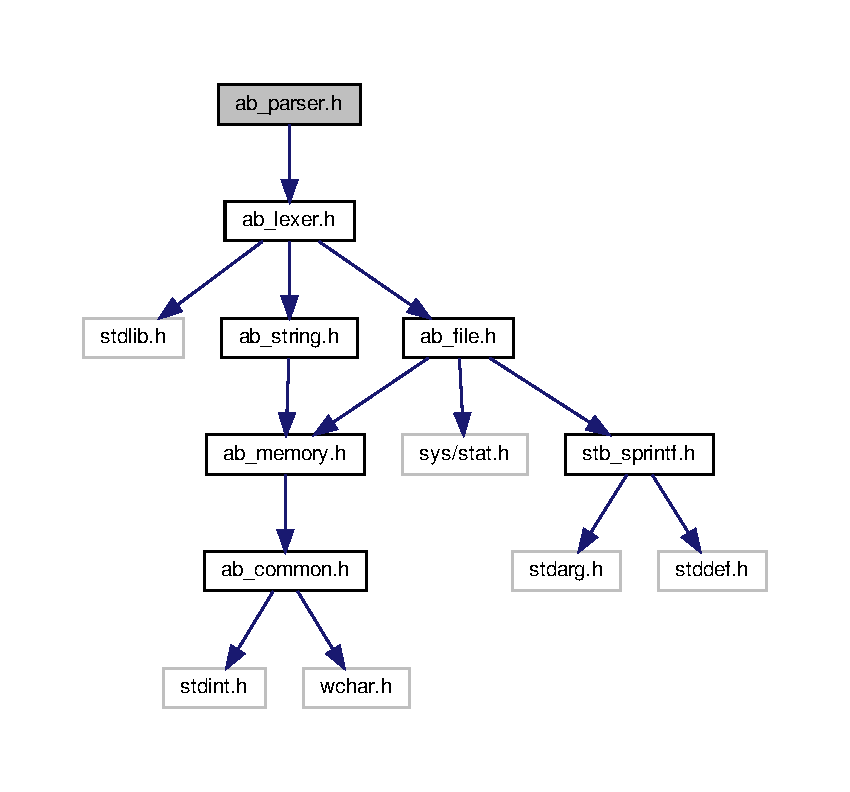
\includegraphics[width=283pt]{d5/d94/ab__parser_8h__incl}
\end{center}
\end{figure}
This graph shows which files directly or indirectly include this file\+:
\nopagebreak
\begin{figure}[H]
\begin{center}
\leavevmode
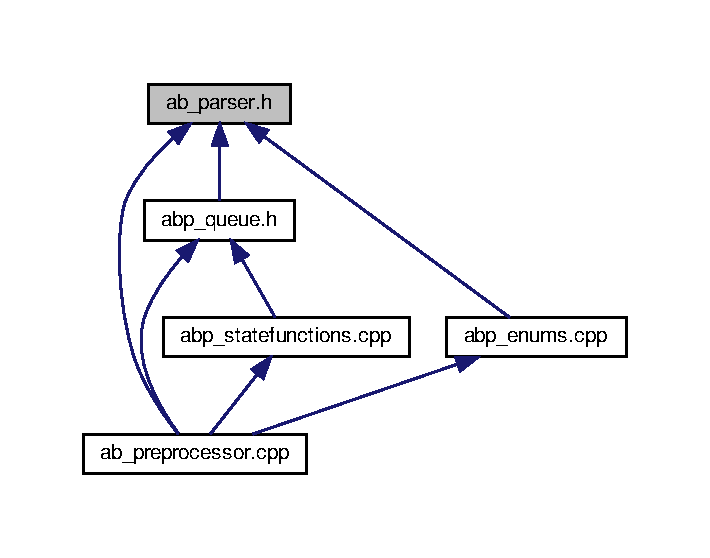
\includegraphics[width=341pt]{d9/da1/ab__parser_8h__dep__incl}
\end{center}
\end{figure}
\subsection*{Classes}
\begin{DoxyCompactItemize}
\item 
struct \hyperlink{structtag}{tag}
\item 
struct \hyperlink{structterm__typeexpr}{term\+\_\+typeexpr}
\item 
struct \hyperlink{structterm__definedfunction}{term\+\_\+definedfunction}
\item 
struct \hyperlink{structterm__statemachine}{term\+\_\+statemachine}
\item 
struct \hyperlink{structterm__structitem}{term\+\_\+structitem}
\item 
struct \hyperlink{structterm__struct}{term\+\_\+struct}
\item 
struct \hyperlink{structterm__enumitem}{term\+\_\+enumitem}
\item 
struct \hyperlink{structterm__enum}{term\+\_\+enum}
\item 
struct \hyperlink{structterm__function}{term\+\_\+function}
\item 
struct \hyperlink{structterm__statefunction}{term\+\_\+statefunction}
\item 
struct \hyperlink{structparser}{parser}
\item 
struct \hyperlink{structoutput__data}{output\+\_\+data}
\end{DoxyCompactItemize}
\subsection*{Macros}
\begin{DoxyCompactItemize}
\item 
\#define \hyperlink{ab__parser_8h_aeabe8109eddf86b30deefb9d28837243}{Init\+List}(Sentinal)
\item 
\#define \hyperlink{ab__parser_8h_a5716e375532c2d8f503025f9deb10593}{Push\+Onto\+List}(Sentinal,  New\+Item)
\item 
\#define \hyperlink{ab__parser_8h_ad6441f2fd946e5baefda8733bc8ed744}{Push\+List\+Onto\+List}(To\+Sentinal,  From\+Sentinal)
\end{DoxyCompactItemize}
\subsection*{Enumerations}
\begin{DoxyCompactItemize}
\item 
enum \hyperlink{ab__parser_8h_ac9039717ce4cccacf493ee306650a423}{custom\+\_\+type} \{ \newline
\hyperlink{ab__parser_8h_ac9039717ce4cccacf493ee306650a423a365c11b5fcf955d07d55c017767c4658}{C\+T\+\_\+\+None}, 
\hyperlink{ab__parser_8h_ac9039717ce4cccacf493ee306650a423a5d9c6244fb2275c721f1f348559f2c41}{C\+T\+\_\+\+Struct}, 
\hyperlink{ab__parser_8h_ac9039717ce4cccacf493ee306650a423a0168fb837b6dd0ef60f59281336f297e}{C\+T\+\_\+\+Union}, 
\hyperlink{ab__parser_8h_ac9039717ce4cccacf493ee306650a423a48f97ab3d4222611634d568b2b11fd9f}{C\+T\+\_\+\+Class}, 
\newline
\hyperlink{ab__parser_8h_ac9039717ce4cccacf493ee306650a423a45908c6d305646ca2e5e6395752c91d3}{C\+T\+\_\+\+Enum}
 \}
\end{DoxyCompactItemize}
\subsection*{Functions}
\begin{DoxyCompactItemize}
\item 
\hyperlink{structtag}{tag} \hyperlink{ab__parser_8h_a2087ae02cf60801129cd945b8a053a01}{Parse\+Tag} (\hyperlink{structlexer}{lexer} $\ast$Lexer, \hyperlink{structparser}{parser} $\ast$Parser)
\end{DoxyCompactItemize}


\subsection{Macro Definition Documentation}
\mbox{\Hypertarget{ab__parser_8h_aeabe8109eddf86b30deefb9d28837243}\label{ab__parser_8h_aeabe8109eddf86b30deefb9d28837243}} 
\index{ab\+\_\+parser.\+h@{ab\+\_\+parser.\+h}!Init\+List@{Init\+List}}
\index{Init\+List@{Init\+List}!ab\+\_\+parser.\+h@{ab\+\_\+parser.\+h}}
\subsubsection{\texorpdfstring{Init\+List}{InitList}}
{\footnotesize\ttfamily \#define Init\+List(\begin{DoxyParamCaption}\item[{}]{Sentinal }\end{DoxyParamCaption})}

{\bfseries Value\+:}
\begin{DoxyCode}
\{ \(\backslash\)
Sentinal.Next = &Sentinal; \(\backslash\)
Sentinal.Prev = &Sentinal; \(\backslash\)
\}
\end{DoxyCode}
\mbox{\Hypertarget{ab__parser_8h_ad6441f2fd946e5baefda8733bc8ed744}\label{ab__parser_8h_ad6441f2fd946e5baefda8733bc8ed744}} 
\index{ab\+\_\+parser.\+h@{ab\+\_\+parser.\+h}!Push\+List\+Onto\+List@{Push\+List\+Onto\+List}}
\index{Push\+List\+Onto\+List@{Push\+List\+Onto\+List}!ab\+\_\+parser.\+h@{ab\+\_\+parser.\+h}}
\subsubsection{\texorpdfstring{Push\+List\+Onto\+List}{PushListOntoList}}
{\footnotesize\ttfamily \#define Push\+List\+Onto\+List(\begin{DoxyParamCaption}\item[{}]{To\+Sentinal,  }\item[{}]{From\+Sentinal }\end{DoxyParamCaption})}

{\bfseries Value\+:}
\begin{DoxyCode}
\{ \(\backslash\)
FromSentinal.Prev->Next = &ToSentinal; \(\backslash\)
FromSentinal.Next->Prev = ToSentinal.Prev; \(\backslash\)
ToSentinal.Prev->Next = FromSentinal.Next; \(\backslash\)
ToSentinal.Prev = FromSentinal.Prev; \(\backslash\)
\}
\end{DoxyCode}
\mbox{\Hypertarget{ab__parser_8h_a5716e375532c2d8f503025f9deb10593}\label{ab__parser_8h_a5716e375532c2d8f503025f9deb10593}} 
\index{ab\+\_\+parser.\+h@{ab\+\_\+parser.\+h}!Push\+Onto\+List@{Push\+Onto\+List}}
\index{Push\+Onto\+List@{Push\+Onto\+List}!ab\+\_\+parser.\+h@{ab\+\_\+parser.\+h}}
\subsubsection{\texorpdfstring{Push\+Onto\+List}{PushOntoList}}
{\footnotesize\ttfamily \#define Push\+Onto\+List(\begin{DoxyParamCaption}\item[{}]{Sentinal,  }\item[{}]{New\+Item }\end{DoxyParamCaption})}

{\bfseries Value\+:}
\begin{DoxyCode}
\{ \(\backslash\)
NewItem->Next = &Sentinal; \(\backslash\)
NewItem->Prev = Sentinal.Prev; \(\backslash\)
Sentinal.Prev->Next = NewItem; \(\backslash\)
Sentinal.Prev = NewItem; \(\backslash\)
\}
\end{DoxyCode}


\subsection{Enumeration Type Documentation}
\mbox{\Hypertarget{ab__parser_8h_ac9039717ce4cccacf493ee306650a423}\label{ab__parser_8h_ac9039717ce4cccacf493ee306650a423}} 
\index{ab\+\_\+parser.\+h@{ab\+\_\+parser.\+h}!custom\+\_\+type@{custom\+\_\+type}}
\index{custom\+\_\+type@{custom\+\_\+type}!ab\+\_\+parser.\+h@{ab\+\_\+parser.\+h}}
\subsubsection{\texorpdfstring{custom\+\_\+type}{custom\_type}}
{\footnotesize\ttfamily enum \hyperlink{ab__parser_8h_ac9039717ce4cccacf493ee306650a423}{custom\+\_\+type}}

\begin{DoxyEnumFields}{Enumerator}
\raisebox{\heightof{T}}[0pt][0pt]{\index{C\+T\+\_\+\+None@{C\+T\+\_\+\+None}!ab\+\_\+parser.\+h@{ab\+\_\+parser.\+h}}\index{ab\+\_\+parser.\+h@{ab\+\_\+parser.\+h}!C\+T\+\_\+\+None@{C\+T\+\_\+\+None}}}\mbox{\Hypertarget{ab__parser_8h_ac9039717ce4cccacf493ee306650a423a365c11b5fcf955d07d55c017767c4658}\label{ab__parser_8h_ac9039717ce4cccacf493ee306650a423a365c11b5fcf955d07d55c017767c4658}} 
C\+T\+\_\+\+None&\\
\hline

\raisebox{\heightof{T}}[0pt][0pt]{\index{C\+T\+\_\+\+Struct@{C\+T\+\_\+\+Struct}!ab\+\_\+parser.\+h@{ab\+\_\+parser.\+h}}\index{ab\+\_\+parser.\+h@{ab\+\_\+parser.\+h}!C\+T\+\_\+\+Struct@{C\+T\+\_\+\+Struct}}}\mbox{\Hypertarget{ab__parser_8h_ac9039717ce4cccacf493ee306650a423a5d9c6244fb2275c721f1f348559f2c41}\label{ab__parser_8h_ac9039717ce4cccacf493ee306650a423a5d9c6244fb2275c721f1f348559f2c41}} 
C\+T\+\_\+\+Struct&\\
\hline

\raisebox{\heightof{T}}[0pt][0pt]{\index{C\+T\+\_\+\+Union@{C\+T\+\_\+\+Union}!ab\+\_\+parser.\+h@{ab\+\_\+parser.\+h}}\index{ab\+\_\+parser.\+h@{ab\+\_\+parser.\+h}!C\+T\+\_\+\+Union@{C\+T\+\_\+\+Union}}}\mbox{\Hypertarget{ab__parser_8h_ac9039717ce4cccacf493ee306650a423a0168fb837b6dd0ef60f59281336f297e}\label{ab__parser_8h_ac9039717ce4cccacf493ee306650a423a0168fb837b6dd0ef60f59281336f297e}} 
C\+T\+\_\+\+Union&\\
\hline

\raisebox{\heightof{T}}[0pt][0pt]{\index{C\+T\+\_\+\+Class@{C\+T\+\_\+\+Class}!ab\+\_\+parser.\+h@{ab\+\_\+parser.\+h}}\index{ab\+\_\+parser.\+h@{ab\+\_\+parser.\+h}!C\+T\+\_\+\+Class@{C\+T\+\_\+\+Class}}}\mbox{\Hypertarget{ab__parser_8h_ac9039717ce4cccacf493ee306650a423a48f97ab3d4222611634d568b2b11fd9f}\label{ab__parser_8h_ac9039717ce4cccacf493ee306650a423a48f97ab3d4222611634d568b2b11fd9f}} 
C\+T\+\_\+\+Class&\\
\hline

\raisebox{\heightof{T}}[0pt][0pt]{\index{C\+T\+\_\+\+Enum@{C\+T\+\_\+\+Enum}!ab\+\_\+parser.\+h@{ab\+\_\+parser.\+h}}\index{ab\+\_\+parser.\+h@{ab\+\_\+parser.\+h}!C\+T\+\_\+\+Enum@{C\+T\+\_\+\+Enum}}}\mbox{\Hypertarget{ab__parser_8h_ac9039717ce4cccacf493ee306650a423a45908c6d305646ca2e5e6395752c91d3}\label{ab__parser_8h_ac9039717ce4cccacf493ee306650a423a45908c6d305646ca2e5e6395752c91d3}} 
C\+T\+\_\+\+Enum&\\
\hline

\end{DoxyEnumFields}


\subsection{Function Documentation}
\mbox{\Hypertarget{ab__parser_8h_a2087ae02cf60801129cd945b8a053a01}\label{ab__parser_8h_a2087ae02cf60801129cd945b8a053a01}} 
\index{ab\+\_\+parser.\+h@{ab\+\_\+parser.\+h}!Parse\+Tag@{Parse\+Tag}}
\index{Parse\+Tag@{Parse\+Tag}!ab\+\_\+parser.\+h@{ab\+\_\+parser.\+h}}
\subsubsection{\texorpdfstring{Parse\+Tag()}{ParseTag()}}
{\footnotesize\ttfamily \hyperlink{structtag}{tag} Parse\+Tag (\begin{DoxyParamCaption}\item[{\hyperlink{structlexer}{lexer} $\ast$}]{Lexer,  }\item[{\hyperlink{structparser}{parser} $\ast$}]{Parser }\end{DoxyParamCaption})}


\hypertarget{ab__preprocessor_8cpp}{}\doxysection{ab\+\_\+preprocessor.\+cpp File Reference}
\label{ab__preprocessor_8cpp}\index{ab\_preprocessor.cpp@{ab\_preprocessor.cpp}}


A basic preprocessor to generate a header file.  


{\ttfamily \#include $<$stdio.\+h$>$}\newline
{\ttfamily \#include $<$time.\+h$>$}\newline
{\ttfamily \#include \char`\"{}ab\+\_\+common.\+h\char`\"{}}\newline
{\ttfamily \#include \char`\"{}ab\+\_\+memory.\+h\char`\"{}}\newline
{\ttfamily \#include \char`\"{}ab\+\_\+string.\+h\char`\"{}}\newline
{\ttfamily \#include \char`\"{}ab\+\_\+file.\+h\char`\"{}}\newline
{\ttfamily \#include \char`\"{}ab\+\_\+lexer.\+h\char`\"{}}\newline
{\ttfamily \#include \char`\"{}ab\+\_\+parser.\+h\char`\"{}}\newline
{\ttfamily \#include \char`\"{}stb\+\_\+sprintf.\+h\char`\"{}}\newline
{\ttfamily \#include \char`\"{}abp\+\_\+queue.\+h\char`\"{}}\newline
{\ttfamily \#include \char`\"{}abp\+\_\+enums.\+cpp\char`\"{}}\newline
{\ttfamily \#include \char`\"{}abp\+\_\+statefunctions.\+cpp\char`\"{}}\newline
{\ttfamily \#include \char`\"{}abp\+\_\+structs.\+cpp\char`\"{}}\newline
Include dependency graph for ab\+\_\+preprocessor.\+cpp\+:\nopagebreak
\begin{figure}[H]
\begin{center}
\leavevmode
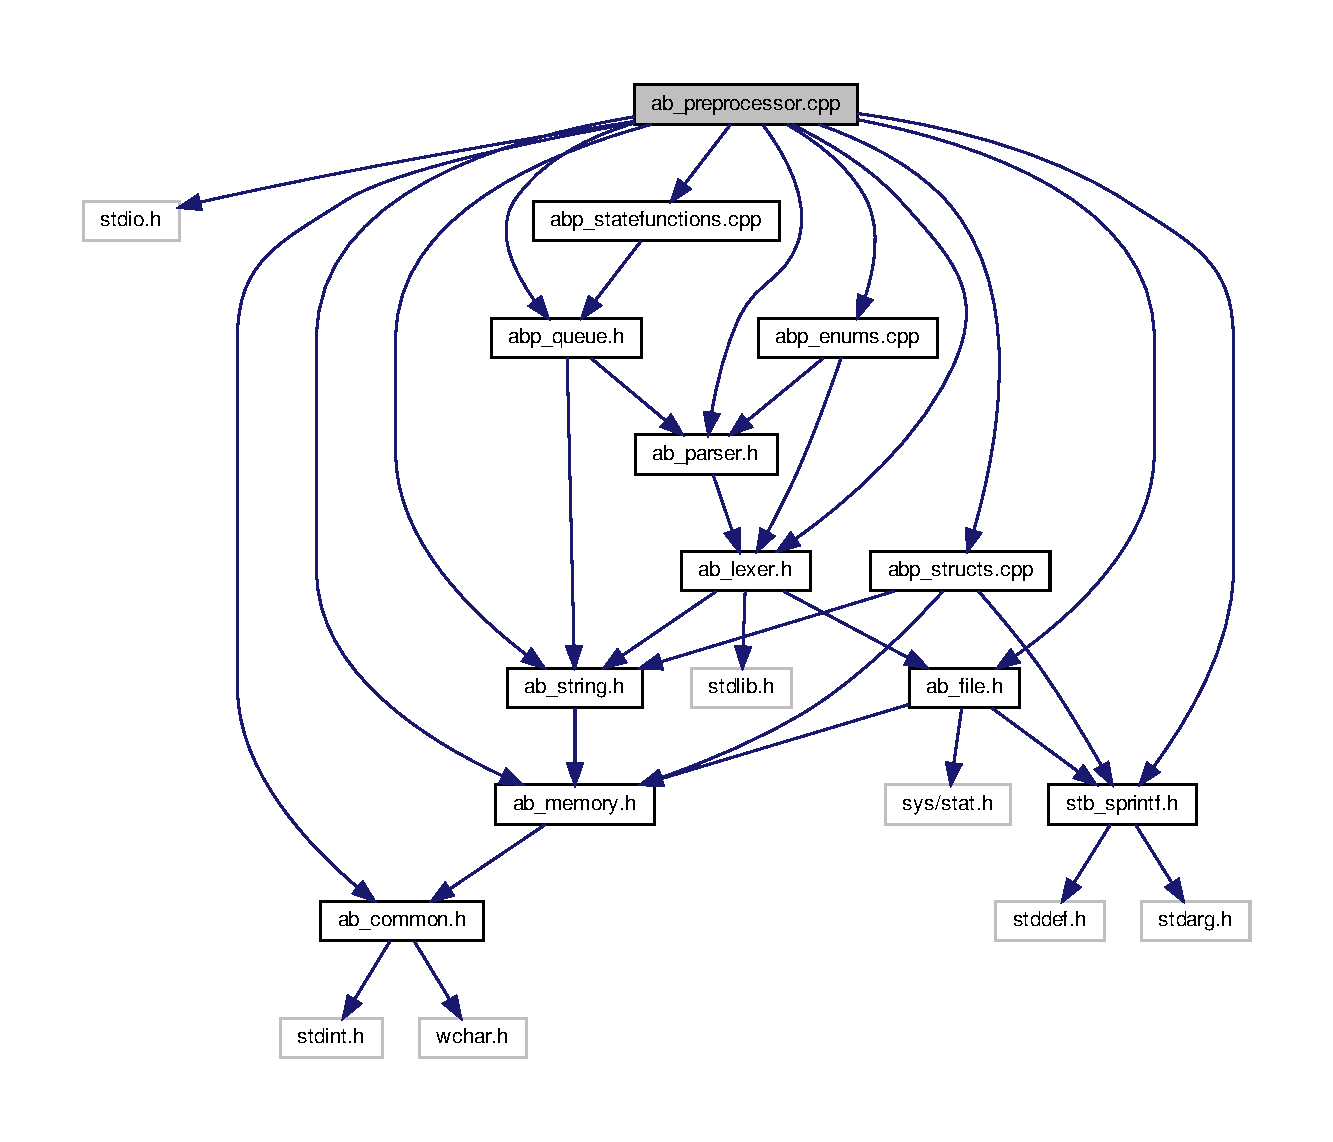
\includegraphics[width=350pt]{d5/d78/ab__preprocessor_8cpp__incl}
\end{center}
\end{figure}
\doxysubsection*{Macros}
\begin{DoxyCompactItemize}
\item 
\#define \mbox{\hyperlink{ab__preprocessor_8cpp_a1c6d5de492ac61ad29aec7aa9a436bbf}{V\+E\+R\+S\+I\+ON}}~\char`\"{}1.\+0\char`\"{}
\item 
\#define \mbox{\hyperlink{ab__preprocessor_8cpp_a912cf300a2ea45ef953fdbd09013ff2f}{M\+E\+M\+O\+R\+Y\+\_\+\+S\+RC}}
\item 
\#define \mbox{\hyperlink{ab__preprocessor_8cpp_a6bb51ed2ff4eb52256ab43148cb826aa}{S\+T\+R\+I\+N\+G\+\_\+\+S\+RC}}
\item 
\#define \mbox{\hyperlink{ab__preprocessor_8cpp_ac56ca87f735628b6d1db0d34f25978ea}{A\+B\+\_\+\+F\+I\+L\+E\+\_\+\+S\+RC}}
\item 
\#define \mbox{\hyperlink{ab__preprocessor_8cpp_a2affa792e6608b227a3545165d400000}{A\+B\+\_\+\+L\+E\+X\+E\+R\+\_\+\+S\+RC}}
\item 
\#define \mbox{\hyperlink{ab__preprocessor_8cpp_ac4d4c61013514e012213131cfef4ce1e}{A\+B\+\_\+\+P\+A\+R\+S\+E\+R\+\_\+\+S\+RC}}
\item 
\#define \mbox{\hyperlink{ab__preprocessor_8cpp_a840dcc5088daf9a542cceb05e306855c}{S\+T\+B\+\_\+\+S\+P\+R\+I\+N\+T\+F\+\_\+\+I\+M\+P\+L\+E\+M\+E\+N\+T\+A\+T\+I\+ON}}
\item 
\#define \mbox{\hyperlink{ab__preprocessor_8cpp_ab8a73ef02993098f2a7b728281f7922e}{A\+B\+P\+\_\+\+Q\+U\+E\+U\+E\+\_\+\+S\+RC}}
\end{DoxyCompactItemize}
\doxysubsection*{Functions}
\begin{DoxyCompactItemize}
\item 
void \mbox{\hyperlink{ab__preprocessor_8cpp_a1ceb4d4f9c01cff4e92adcca4d31949f}{Write\+To\+Output}} (\mbox{\hyperlink{structoutput__data}{output\+\_\+data}} $\ast$Output, memory\+\_\+arena $\ast$Memory, char const $\ast$String,...)
\item 
void \mbox{\hyperlink{ab__preprocessor_8cpp_a543263769375c19c9f59fe002d5e50ef}{Copy\+To\+Output}} (\mbox{\hyperlink{structoutput__data}{output\+\_\+data}} $\ast$Output, memory\+\_\+arena $\ast$Memory, char const $\ast$String)
\item 
void \mbox{\hyperlink{ab__preprocessor_8cpp_a8f1cafd703a8d82c50649694e22999bd}{Copy\+To\+Output}} (\mbox{\hyperlink{structoutput__data}{output\+\_\+data}} $\ast$To\+Output, memory\+\_\+arena $\ast$Memory, \mbox{\hyperlink{structoutput__data}{output\+\_\+data}} $\ast$From\+Output)
\item 
\mbox{\hyperlink{structoutput__data}{output\+\_\+data}} $\ast$ \mbox{\hyperlink{ab__preprocessor_8cpp_a3eed7463a6e214d1f4cf577811607834}{Generate\+Output}} (memory\+\_\+arena $\ast$Memory, char const $\ast$Output\+File, \mbox{\hyperlink{structoutput__data}{output\+\_\+data}} $\ast$Header\+Includes, \mbox{\hyperlink{structoutput__data}{output\+\_\+data}} $\ast$Header, \mbox{\hyperlink{structoutput__data}{output\+\_\+data}} $\ast$Definition)
\item 
void \mbox{\hyperlink{ab__preprocessor_8cpp_a64d78688e6ec9c0c314050130b29d06b}{Create\+Full\+Filename}} (char $\ast$Output, size\+\_\+t Max\+Length, char const $\ast$Path, u32 Number)
\begin{DoxyCompactList}\small\item\em Write out file. \end{DoxyCompactList}\item 
void \mbox{\hyperlink{ab__preprocessor_8cpp_a2015c745c296d4961772e6f3bb73f7be}{Write\+Output\+To\+File}} (\mbox{\hyperlink{structoutput__data}{output\+\_\+data}} $\ast$Output\+Data, char const $\ast$Source\+Directory, char const $\ast$Output\+File)
\item 
void \mbox{\hyperlink{ab__preprocessor_8cpp_aa5d09e49545215d26b1b3a7f7044f79e}{Write\+Output\+To\+Std\+Out}} (\mbox{\hyperlink{structoutput__data}{output\+\_\+data}} $\ast$Output\+Data)
\begin{DoxyCompactList}\small\item\em Write out to screen. \end{DoxyCompactList}\item 
int \mbox{\hyperlink{ab__preprocessor_8cpp_a3c04138a5bfe5d72780bb7e82a18e627}{main}} (int argc, char $\ast$$\ast$argv)
\end{DoxyCompactItemize}
\doxysubsection*{Variables}
\begin{DoxyCompactItemize}
\item 
char const  $\ast$ \mbox{\hyperlink{ab__preprocessor_8cpp_af946521958bb4da2ca5af31b7b9d67c7}{Generated\+Tag}} = \char`\"{}/$\ast$ $\ast$ G\+E\+N\+E\+R\+A\+T\+ED $\ast$ $\ast$/\char`\"{}
\end{DoxyCompactItemize}


\doxysubsection{Detailed Description}
A basic preprocessor to generate a header file. 

\begin{DoxyAuthor}{Author}
Amos Buchanan 
\end{DoxyAuthor}
\begin{DoxyVersion}{Version}
1.\+0 
\end{DoxyVersion}
\begin{DoxyDate}{Date}
2020 
\end{DoxyDate}
\begin{DoxyCopyright}{Copyright}
\href{https://opensource.org/licenses/MIT}{\texttt{ M\+IT Public License}}
\end{DoxyCopyright}
This is a basic pre-\/preprocessor that reads in the source files in a directory and outputs a generated source file with a number of standard functions. For usage, see the project \mbox{\hyperlink{Readme_8md}{Readme.\+md}} file.\hypertarget{ab__preprocessor_8cpp_autotoc_md1}{}\doxysubsection{M\+I\+T License}\label{ab__preprocessor_8cpp_autotoc_md1}
\href{https://opensource.org/licenses/MIT}{\texttt{ M\+IT Public License}}

Copyright 2020 Amos Buchanan

Permission is hereby granted, free of charge, to any person obtaining a copy of this software and associated documentation files (the \char`\"{}\+Software\char`\"{}), to deal in the Software without restriction, including without limitation the rights to use, copy, modify, merge, publish, distribute, sublicense, and/or sell copies of the Software, and to permit persons to whom the Software is furnished to do so, subject to the following conditions\+:

The above copyright notice and this permission notice shall be included in all copies or substantial portions of the Software.

T\+HE S\+O\+F\+T\+W\+A\+RE IS P\+R\+O\+V\+I\+D\+ED \char`\"{}\+A\+S I\+S\char`\"{}, W\+I\+T\+H\+O\+UT W\+A\+R\+R\+A\+N\+TY OF A\+NY K\+I\+ND, E\+X\+P\+R\+E\+SS OR I\+M\+P\+L\+I\+ED, I\+N\+C\+L\+U\+D\+I\+NG B\+UT N\+OT L\+I\+M\+I\+T\+ED TO T\+HE W\+A\+R\+R\+A\+N\+T\+I\+ES OF M\+E\+R\+C\+H\+A\+N\+T\+A\+B\+I\+L\+I\+TY, F\+I\+T\+N\+E\+SS F\+OR A P\+A\+R\+T\+I\+C\+U\+L\+AR P\+U\+R\+P\+O\+SE A\+ND N\+O\+N\+I\+N\+F\+R\+I\+N\+G\+E\+M\+E\+NT. IN NO E\+V\+E\+NT S\+H\+A\+LL T\+HE A\+U\+T\+H\+O\+RS OR C\+O\+P\+Y\+R\+I\+G\+HT H\+O\+L\+D\+E\+RS BE L\+I\+A\+B\+LE F\+OR A\+NY C\+L\+A\+IM, D\+A\+M\+A\+G\+ES OR O\+T\+H\+ER L\+I\+A\+B\+I\+L\+I\+TY, W\+H\+E\+T\+H\+ER IN AN A\+C\+T\+I\+ON OF C\+O\+N\+T\+R\+A\+CT, T\+O\+RT OR O\+T\+H\+E\+R\+W\+I\+SE, A\+R\+I\+S\+I\+NG F\+R\+OM, O\+UT OF OR IN C\+O\+N\+N\+E\+C\+T\+I\+ON W\+I\+TH T\+HE S\+O\+F\+T\+W\+A\+RE OR T\+HE U\+SE OR O\+T\+H\+ER D\+E\+A\+L\+I\+N\+GS IN T\+HE S\+O\+F\+T\+W\+A\+RE. 

\doxysubsection{Macro Definition Documentation}
\mbox{\Hypertarget{ab__preprocessor_8cpp_ac56ca87f735628b6d1db0d34f25978ea}\label{ab__preprocessor_8cpp_ac56ca87f735628b6d1db0d34f25978ea}} 
\index{ab\_preprocessor.cpp@{ab\_preprocessor.cpp}!AB\_FILE\_SRC@{AB\_FILE\_SRC}}
\index{AB\_FILE\_SRC@{AB\_FILE\_SRC}!ab\_preprocessor.cpp@{ab\_preprocessor.cpp}}
\doxysubsubsection{\texorpdfstring{AB\_FILE\_SRC}{AB\_FILE\_SRC}}
{\footnotesize\ttfamily \#define A\+B\+\_\+\+F\+I\+L\+E\+\_\+\+S\+RC}

\mbox{\Hypertarget{ab__preprocessor_8cpp_a2affa792e6608b227a3545165d400000}\label{ab__preprocessor_8cpp_a2affa792e6608b227a3545165d400000}} 
\index{ab\_preprocessor.cpp@{ab\_preprocessor.cpp}!AB\_LEXER\_SRC@{AB\_LEXER\_SRC}}
\index{AB\_LEXER\_SRC@{AB\_LEXER\_SRC}!ab\_preprocessor.cpp@{ab\_preprocessor.cpp}}
\doxysubsubsection{\texorpdfstring{AB\_LEXER\_SRC}{AB\_LEXER\_SRC}}
{\footnotesize\ttfamily \#define A\+B\+\_\+\+L\+E\+X\+E\+R\+\_\+\+S\+RC}

\mbox{\Hypertarget{ab__preprocessor_8cpp_ac4d4c61013514e012213131cfef4ce1e}\label{ab__preprocessor_8cpp_ac4d4c61013514e012213131cfef4ce1e}} 
\index{ab\_preprocessor.cpp@{ab\_preprocessor.cpp}!AB\_PARSER\_SRC@{AB\_PARSER\_SRC}}
\index{AB\_PARSER\_SRC@{AB\_PARSER\_SRC}!ab\_preprocessor.cpp@{ab\_preprocessor.cpp}}
\doxysubsubsection{\texorpdfstring{AB\_PARSER\_SRC}{AB\_PARSER\_SRC}}
{\footnotesize\ttfamily \#define A\+B\+\_\+\+P\+A\+R\+S\+E\+R\+\_\+\+S\+RC}

\mbox{\Hypertarget{ab__preprocessor_8cpp_ab8a73ef02993098f2a7b728281f7922e}\label{ab__preprocessor_8cpp_ab8a73ef02993098f2a7b728281f7922e}} 
\index{ab\_preprocessor.cpp@{ab\_preprocessor.cpp}!ABP\_QUEUE\_SRC@{ABP\_QUEUE\_SRC}}
\index{ABP\_QUEUE\_SRC@{ABP\_QUEUE\_SRC}!ab\_preprocessor.cpp@{ab\_preprocessor.cpp}}
\doxysubsubsection{\texorpdfstring{ABP\_QUEUE\_SRC}{ABP\_QUEUE\_SRC}}
{\footnotesize\ttfamily \#define A\+B\+P\+\_\+\+Q\+U\+E\+U\+E\+\_\+\+S\+RC}

\mbox{\Hypertarget{ab__preprocessor_8cpp_a912cf300a2ea45ef953fdbd09013ff2f}\label{ab__preprocessor_8cpp_a912cf300a2ea45ef953fdbd09013ff2f}} 
\index{ab\_preprocessor.cpp@{ab\_preprocessor.cpp}!MEMORY\_SRC@{MEMORY\_SRC}}
\index{MEMORY\_SRC@{MEMORY\_SRC}!ab\_preprocessor.cpp@{ab\_preprocessor.cpp}}
\doxysubsubsection{\texorpdfstring{MEMORY\_SRC}{MEMORY\_SRC}}
{\footnotesize\ttfamily \#define M\+E\+M\+O\+R\+Y\+\_\+\+S\+RC}

\mbox{\Hypertarget{ab__preprocessor_8cpp_a840dcc5088daf9a542cceb05e306855c}\label{ab__preprocessor_8cpp_a840dcc5088daf9a542cceb05e306855c}} 
\index{ab\_preprocessor.cpp@{ab\_preprocessor.cpp}!STB\_SPRINTF\_IMPLEMENTATION@{STB\_SPRINTF\_IMPLEMENTATION}}
\index{STB\_SPRINTF\_IMPLEMENTATION@{STB\_SPRINTF\_IMPLEMENTATION}!ab\_preprocessor.cpp@{ab\_preprocessor.cpp}}
\doxysubsubsection{\texorpdfstring{STB\_SPRINTF\_IMPLEMENTATION}{STB\_SPRINTF\_IMPLEMENTATION}}
{\footnotesize\ttfamily \#define S\+T\+B\+\_\+\+S\+P\+R\+I\+N\+T\+F\+\_\+\+I\+M\+P\+L\+E\+M\+E\+N\+T\+A\+T\+I\+ON}

\mbox{\Hypertarget{ab__preprocessor_8cpp_a6bb51ed2ff4eb52256ab43148cb826aa}\label{ab__preprocessor_8cpp_a6bb51ed2ff4eb52256ab43148cb826aa}} 
\index{ab\_preprocessor.cpp@{ab\_preprocessor.cpp}!STRING\_SRC@{STRING\_SRC}}
\index{STRING\_SRC@{STRING\_SRC}!ab\_preprocessor.cpp@{ab\_preprocessor.cpp}}
\doxysubsubsection{\texorpdfstring{STRING\_SRC}{STRING\_SRC}}
{\footnotesize\ttfamily \#define S\+T\+R\+I\+N\+G\+\_\+\+S\+RC}

\mbox{\Hypertarget{ab__preprocessor_8cpp_a1c6d5de492ac61ad29aec7aa9a436bbf}\label{ab__preprocessor_8cpp_a1c6d5de492ac61ad29aec7aa9a436bbf}} 
\index{ab\_preprocessor.cpp@{ab\_preprocessor.cpp}!VERSION@{VERSION}}
\index{VERSION@{VERSION}!ab\_preprocessor.cpp@{ab\_preprocessor.cpp}}
\doxysubsubsection{\texorpdfstring{VERSION}{VERSION}}
{\footnotesize\ttfamily \#define V\+E\+R\+S\+I\+ON~\char`\"{}1.\+0\char`\"{}}



\doxysubsection{Function Documentation}
\mbox{\Hypertarget{ab__preprocessor_8cpp_a543263769375c19c9f59fe002d5e50ef}\label{ab__preprocessor_8cpp_a543263769375c19c9f59fe002d5e50ef}} 
\index{ab\_preprocessor.cpp@{ab\_preprocessor.cpp}!CopyToOutput@{CopyToOutput}}
\index{CopyToOutput@{CopyToOutput}!ab\_preprocessor.cpp@{ab\_preprocessor.cpp}}
\doxysubsubsection{\texorpdfstring{CopyToOutput()}{CopyToOutput()}\hspace{0.1cm}{\footnotesize\ttfamily [1/2]}}
{\footnotesize\ttfamily void Copy\+To\+Output (\begin{DoxyParamCaption}\item[{\mbox{\hyperlink{structoutput__data}{output\+\_\+data}} $\ast$}]{Output,  }\item[{memory\+\_\+arena $\ast$}]{Memory,  }\item[{char const $\ast$}]{String }\end{DoxyParamCaption})\hspace{0.3cm}{\ttfamily [inline]}}

\mbox{\Hypertarget{ab__preprocessor_8cpp_a8f1cafd703a8d82c50649694e22999bd}\label{ab__preprocessor_8cpp_a8f1cafd703a8d82c50649694e22999bd}} 
\index{ab\_preprocessor.cpp@{ab\_preprocessor.cpp}!CopyToOutput@{CopyToOutput}}
\index{CopyToOutput@{CopyToOutput}!ab\_preprocessor.cpp@{ab\_preprocessor.cpp}}
\doxysubsubsection{\texorpdfstring{CopyToOutput()}{CopyToOutput()}\hspace{0.1cm}{\footnotesize\ttfamily [2/2]}}
{\footnotesize\ttfamily void Copy\+To\+Output (\begin{DoxyParamCaption}\item[{\mbox{\hyperlink{structoutput__data}{output\+\_\+data}} $\ast$}]{To\+Output,  }\item[{memory\+\_\+arena $\ast$}]{Memory,  }\item[{\mbox{\hyperlink{structoutput__data}{output\+\_\+data}} $\ast$}]{From\+Output }\end{DoxyParamCaption})\hspace{0.3cm}{\ttfamily [inline]}}

\mbox{\Hypertarget{ab__preprocessor_8cpp_a64d78688e6ec9c0c314050130b29d06b}\label{ab__preprocessor_8cpp_a64d78688e6ec9c0c314050130b29d06b}} 
\index{ab\_preprocessor.cpp@{ab\_preprocessor.cpp}!CreateFullFilename@{CreateFullFilename}}
\index{CreateFullFilename@{CreateFullFilename}!ab\_preprocessor.cpp@{ab\_preprocessor.cpp}}
\doxysubsubsection{\texorpdfstring{CreateFullFilename()}{CreateFullFilename()}}
{\footnotesize\ttfamily void Create\+Full\+Filename (\begin{DoxyParamCaption}\item[{char $\ast$}]{Output,  }\item[{size\+\_\+t}]{Max\+Length,  }\item[{char const $\ast$}]{Path,  }\item[{u32}]{Number }\end{DoxyParamCaption})\hspace{0.3cm}{\ttfamily [inline]}}



Write out file. 

\mbox{\Hypertarget{ab__preprocessor_8cpp_a3eed7463a6e214d1f4cf577811607834}\label{ab__preprocessor_8cpp_a3eed7463a6e214d1f4cf577811607834}} 
\index{ab\_preprocessor.cpp@{ab\_preprocessor.cpp}!GenerateOutput@{GenerateOutput}}
\index{GenerateOutput@{GenerateOutput}!ab\_preprocessor.cpp@{ab\_preprocessor.cpp}}
\doxysubsubsection{\texorpdfstring{GenerateOutput()}{GenerateOutput()}}
{\footnotesize\ttfamily \mbox{\hyperlink{structoutput__data}{output\+\_\+data}}$\ast$ Generate\+Output (\begin{DoxyParamCaption}\item[{memory\+\_\+arena $\ast$}]{Memory,  }\item[{char const $\ast$}]{Output\+File,  }\item[{\mbox{\hyperlink{structoutput__data}{output\+\_\+data}} $\ast$}]{Header\+Includes,  }\item[{\mbox{\hyperlink{structoutput__data}{output\+\_\+data}} $\ast$}]{Header,  }\item[{\mbox{\hyperlink{structoutput__data}{output\+\_\+data}} $\ast$}]{Definition }\end{DoxyParamCaption})}

\mbox{\Hypertarget{ab__preprocessor_8cpp_a3c04138a5bfe5d72780bb7e82a18e627}\label{ab__preprocessor_8cpp_a3c04138a5bfe5d72780bb7e82a18e627}} 
\index{ab\_preprocessor.cpp@{ab\_preprocessor.cpp}!main@{main}}
\index{main@{main}!ab\_preprocessor.cpp@{ab\_preprocessor.cpp}}
\doxysubsubsection{\texorpdfstring{main()}{main()}}
{\footnotesize\ttfamily int main (\begin{DoxyParamCaption}\item[{int}]{argc,  }\item[{char $\ast$$\ast$}]{argv }\end{DoxyParamCaption})}

\mbox{\Hypertarget{ab__preprocessor_8cpp_a2015c745c296d4961772e6f3bb73f7be}\label{ab__preprocessor_8cpp_a2015c745c296d4961772e6f3bb73f7be}} 
\index{ab\_preprocessor.cpp@{ab\_preprocessor.cpp}!WriteOutputToFile@{WriteOutputToFile}}
\index{WriteOutputToFile@{WriteOutputToFile}!ab\_preprocessor.cpp@{ab\_preprocessor.cpp}}
\doxysubsubsection{\texorpdfstring{WriteOutputToFile()}{WriteOutputToFile()}}
{\footnotesize\ttfamily void Write\+Output\+To\+File (\begin{DoxyParamCaption}\item[{\mbox{\hyperlink{structoutput__data}{output\+\_\+data}} $\ast$}]{Output\+Data,  }\item[{char const $\ast$}]{Source\+Directory,  }\item[{char const $\ast$}]{Output\+File }\end{DoxyParamCaption})}

\mbox{\Hypertarget{ab__preprocessor_8cpp_aa5d09e49545215d26b1b3a7f7044f79e}\label{ab__preprocessor_8cpp_aa5d09e49545215d26b1b3a7f7044f79e}} 
\index{ab\_preprocessor.cpp@{ab\_preprocessor.cpp}!WriteOutputToStdOut@{WriteOutputToStdOut}}
\index{WriteOutputToStdOut@{WriteOutputToStdOut}!ab\_preprocessor.cpp@{ab\_preprocessor.cpp}}
\doxysubsubsection{\texorpdfstring{WriteOutputToStdOut()}{WriteOutputToStdOut()}}
{\footnotesize\ttfamily void Write\+Output\+To\+Std\+Out (\begin{DoxyParamCaption}\item[{\mbox{\hyperlink{structoutput__data}{output\+\_\+data}} $\ast$}]{Output\+Data }\end{DoxyParamCaption})}



Write out to screen. 

\mbox{\Hypertarget{ab__preprocessor_8cpp_a1ceb4d4f9c01cff4e92adcca4d31949f}\label{ab__preprocessor_8cpp_a1ceb4d4f9c01cff4e92adcca4d31949f}} 
\index{ab\_preprocessor.cpp@{ab\_preprocessor.cpp}!WriteToOutput@{WriteToOutput}}
\index{WriteToOutput@{WriteToOutput}!ab\_preprocessor.cpp@{ab\_preprocessor.cpp}}
\doxysubsubsection{\texorpdfstring{WriteToOutput()}{WriteToOutput()}}
{\footnotesize\ttfamily void Write\+To\+Output (\begin{DoxyParamCaption}\item[{\mbox{\hyperlink{structoutput__data}{output\+\_\+data}} $\ast$}]{Output,  }\item[{memory\+\_\+arena $\ast$}]{Memory,  }\item[{char const $\ast$}]{String,  }\item[{}]{... }\end{DoxyParamCaption})\hspace{0.3cm}{\ttfamily [inline]}}



\doxysubsection{Variable Documentation}
\mbox{\Hypertarget{ab__preprocessor_8cpp_af946521958bb4da2ca5af31b7b9d67c7}\label{ab__preprocessor_8cpp_af946521958bb4da2ca5af31b7b9d67c7}} 
\index{ab\_preprocessor.cpp@{ab\_preprocessor.cpp}!GeneratedTag@{GeneratedTag}}
\index{GeneratedTag@{GeneratedTag}!ab\_preprocessor.cpp@{ab\_preprocessor.cpp}}
\doxysubsubsection{\texorpdfstring{GeneratedTag}{GeneratedTag}}
{\footnotesize\ttfamily char const$\ast$ Generated\+Tag = \char`\"{}/$\ast$ $\ast$ G\+E\+N\+E\+R\+A\+T\+ED $\ast$ $\ast$/\char`\"{}}


\hypertarget{ab__string_8h}{}\doxysection{ab\+\_\+string.\+h File Reference}
\label{ab__string_8h}\index{ab\_string.h@{ab\_string.h}}


Using string fragments, usually but not exclusively sections of larger strings.  


{\ttfamily \#include \char`\"{}ab\+\_\+memory.\+h\char`\"{}}\newline
Include dependency graph for ab\+\_\+string.\+h\+:\nopagebreak
\begin{figure}[H]
\begin{center}
\leavevmode
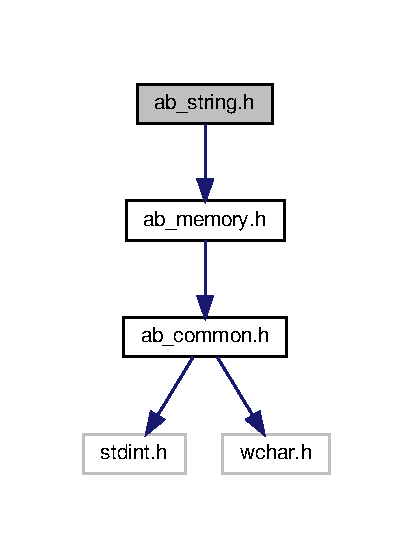
\includegraphics[width=198pt]{de/dc1/ab__string_8h__incl}
\end{center}
\end{figure}
This graph shows which files directly or indirectly include this file\+:\nopagebreak
\begin{figure}[H]
\begin{center}
\leavevmode
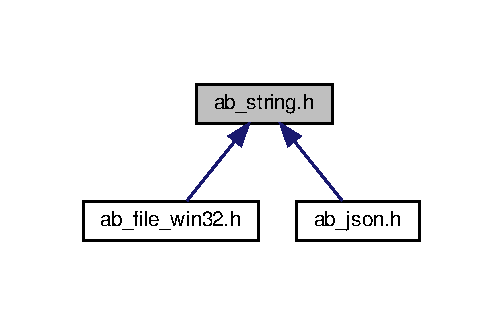
\includegraphics[width=145pt]{df/d7f/ab__string_8h__dep__incl}
\end{center}
\end{figure}
\doxysubsection*{Classes}
\begin{DoxyCompactItemize}
\item 
struct \mbox{\hyperlink{structst__ptr}{st\+\_\+ptr}}
\begin{DoxyCompactList}\small\item\em Pointer and length of a character array. \end{DoxyCompactList}\end{DoxyCompactItemize}
\doxysubsection*{Macros}
\begin{DoxyCompactItemize}
\item 
\#define \mbox{\hyperlink{ab__string_8h_a7f78f576bc59e91ba524ecacde27fb02}{P\+S\+T\+R\+I\+NG}}(S\+TR)~S\+T\+R.\+Length, S\+T\+R.\+String
\begin{DoxyCompactList}\small\item\em Helper to print \mbox{\hyperlink{structst__ptr}{st\+\_\+ptr}}. \end{DoxyCompactList}\end{DoxyCompactItemize}
\doxysubsection*{Functions}
\begin{DoxyCompactItemize}
\item 
\mbox{\hyperlink{ab__common_8h_afaa62991928fb9fb18ff0db62a040aba}{u32}} \mbox{\hyperlink{ab__string_8h_ac07424bcd3602591f8421bed6ca226cc}{st\+\_\+\+String\+Length}} (char const $\ast$x, \mbox{\hyperlink{ab__common_8h_afaa62991928fb9fb18ff0db62a040aba}{u32}} Max\+Length)
\begin{DoxyCompactList}\small\item\em Get the length of a null-\/terminated string. \end{DoxyCompactList}\item 
\mbox{\hyperlink{ab__common_8h_a70e369648385b50f2d0588e8e8745275}{b8}} \mbox{\hyperlink{ab__string_8h_ac86287d9d07821dfc6b740f0ebc03e7d}{st\+\_\+\+Are\+Strings\+Equal}} (char const $\ast$String1, char const $\ast$String2, \mbox{\hyperlink{ab__common_8h_afaa62991928fb9fb18ff0db62a040aba}{u32}} Max\+Length, \mbox{\hyperlink{ab__common_8h_a70e369648385b50f2d0588e8e8745275}{b8}} is\+Case\+Insensitive)
\begin{DoxyCompactList}\small\item\em Compare two strings. \end{DoxyCompactList}\item 
\mbox{\hyperlink{ab__common_8h_a70e369648385b50f2d0588e8e8745275}{b8}} \mbox{\hyperlink{ab__string_8h_ab3cb2a132e3a3b4e219bb2242a94928f}{st\+\_\+\+Are\+Strings\+Equal}} (const char $\ast$String1, \mbox{\hyperlink{ab__common_8h_afaa62991928fb9fb18ff0db62a040aba}{u32}} String1\+Len, const char $\ast$String2, \mbox{\hyperlink{ab__common_8h_afaa62991928fb9fb18ff0db62a040aba}{u32}} String2\+Len, \mbox{\hyperlink{ab__common_8h_a70e369648385b50f2d0588e8e8745275}{b8}} is\+Case\+Insensitive)
\begin{DoxyCompactList}\small\item\em Compare two strings. \end{DoxyCompactList}\item 
\mbox{\hyperlink{ab__common_8h_a70e369648385b50f2d0588e8e8745275}{b8}} \mbox{\hyperlink{ab__string_8h_a71d738c82a030990ac4cd11228187aed}{st\+\_\+\+Are\+Strings\+Equal}} (char const $\ast$String1, \mbox{\hyperlink{ab__common_8h_afaa62991928fb9fb18ff0db62a040aba}{u32}} String1\+Len, char const $\ast$String2, \mbox{\hyperlink{ab__common_8h_afaa62991928fb9fb18ff0db62a040aba}{u32}} String2\+Len)
\begin{DoxyCompactList}\small\item\em Compare two strings. \end{DoxyCompactList}\item 
\mbox{\hyperlink{ab__common_8h_a70e369648385b50f2d0588e8e8745275}{b8}} \mbox{\hyperlink{ab__string_8h_a1933d349d4f32a3b49e5f4364a56b4e6}{st\+\_\+\+Are\+Strings\+Equal}} (\mbox{\hyperlink{structst__ptr}{st\+\_\+ptr}} String1, \mbox{\hyperlink{structst__ptr}{st\+\_\+ptr}} String2)
\begin{DoxyCompactList}\small\item\em Compare two {\ttfamily \mbox{\hyperlink{structst__ptr}{st\+\_\+ptr}}}. \end{DoxyCompactList}\item 
\mbox{\hyperlink{ab__common_8h_a70e369648385b50f2d0588e8e8745275}{b8}} \mbox{\hyperlink{ab__string_8h_a0a7381b99009fa1cd3ecd46cf5de2c88}{st\+\_\+\+Are\+Strings\+Equal}} (char const $\ast$String, \mbox{\hyperlink{ab__common_8h_afaa62991928fb9fb18ff0db62a040aba}{u32}} String\+Len, \mbox{\hyperlink{structst__ptr}{st\+\_\+ptr}} String\+Ptr)
\begin{DoxyCompactList}\small\item\em Compare a null-\/terminated string with a {\ttfamily \mbox{\hyperlink{structst__ptr}{st\+\_\+ptr}}}. \end{DoxyCompactList}\item 
\mbox{\hyperlink{ab__common_8h_ae9b1af5c037e57a98884758875d3a7c4}{s32}} \mbox{\hyperlink{ab__string_8h_a1a043a15b730b8d058445c28cede1906}{st\+\_\+\+Find\+In\+List}} (\mbox{\hyperlink{structst__ptr}{st\+\_\+ptr}} String, \mbox{\hyperlink{ab__common_8h_afaa62991928fb9fb18ff0db62a040aba}{u32}} List\+Count, const \mbox{\hyperlink{structst__ptr}{st\+\_\+ptr}} $\ast$List, \mbox{\hyperlink{ab__common_8h_a70e369648385b50f2d0588e8e8745275}{b8}} is\+Case\+Insensitive=false)
\begin{DoxyCompactList}\small\item\em Find a string in a list of strings. \end{DoxyCompactList}\item 
\mbox{\hyperlink{ab__common_8h_ae9b1af5c037e57a98884758875d3a7c4}{s32}} \mbox{\hyperlink{ab__string_8h_a988b3993f14543652378ae4b915e1e15}{st\+\_\+\+Find\+In\+List}} (const char $\ast$Search\+String, \mbox{\hyperlink{ab__common_8h_afaa62991928fb9fb18ff0db62a040aba}{u32}} List\+Count, const \mbox{\hyperlink{structst__ptr}{st\+\_\+ptr}} $\ast$List, \mbox{\hyperlink{ab__common_8h_a70e369648385b50f2d0588e8e8745275}{b8}} is\+Case\+Insensitive=false)
\begin{DoxyCompactList}\small\item\em Find a string in a list of strings. \end{DoxyCompactList}\item 
\mbox{\hyperlink{ab__common_8h_afaa62991928fb9fb18ff0db62a040aba}{u32}} \mbox{\hyperlink{ab__string_8h_a3bb4db362b23466a8a4ec56f4cc82816}{st\+\_\+\+String\+Copy}} (char $\ast$Dest\+String, const char $\ast$Src\+String, size\+\_\+t Length, \mbox{\hyperlink{ab__common_8h_a70e369648385b50f2d0588e8e8745275}{b8}} Add\+Terminator)
\begin{DoxyCompactList}\small\item\em Safe null-\/terminated string copy. \end{DoxyCompactList}\item 
\mbox{\hyperlink{structst__ptr}{st\+\_\+ptr}} \mbox{\hyperlink{ab__string_8h_a954364e0fd13aaca0011607310d8b455}{st\+\_\+\+Create\+String\+Ptr}} (memory\+\_\+arena $\ast$Memory, const char $\ast$String)
\begin{DoxyCompactList}\small\item\em Create a string pointer out of a string. \end{DoxyCompactList}\item 
\mbox{\hyperlink{structst__ptr}{st\+\_\+ptr}} \mbox{\hyperlink{ab__string_8h_acca3ec335b387116dc3bae074f9655d1}{Create\+String\+Ptr}} (char const $\ast$String, \mbox{\hyperlink{ab__common_8h_afaa62991928fb9fb18ff0db62a040aba}{u32}} Length)
\begin{DoxyCompactList}\small\item\em Create a string pointer out of a constant string. \end{DoxyCompactList}\end{DoxyCompactItemize}


\doxysubsection{Detailed Description}
Using string fragments, usually but not exclusively sections of larger strings. 

\begin{DoxyAuthor}{Author}
Amos Buchanan 
\end{DoxyAuthor}
\begin{DoxyVersion}{Version}
1.\+0 
\end{DoxyVersion}
\begin{DoxyDate}{Date}
2020
\end{DoxyDate}
These are functions to handle string fragments. There are also some safe string copy and find functions. {\ttfamily \mbox{\hyperlink{structst__ptr}{st\+\_\+ptr}}} is generally used for a fragment of a larger piece of text.

This is a single-\/file library. You may include it as a header just as any other. Add the following define to include the source {\itshape once} per project\+:


\begin{DoxyCode}{0}
\DoxyCodeLine{\textcolor{preprocessor}{\#define STRING\_SRC}}
\DoxyCodeLine{\textcolor{preprocessor}{\#include "{}ab\_string.h"{}}}
\end{DoxyCode}
 

\doxysubsection{Macro Definition Documentation}
\mbox{\Hypertarget{ab__string_8h_a7f78f576bc59e91ba524ecacde27fb02}\label{ab__string_8h_a7f78f576bc59e91ba524ecacde27fb02}} 
\index{ab\_string.h@{ab\_string.h}!PSTRING@{PSTRING}}
\index{PSTRING@{PSTRING}!ab\_string.h@{ab\_string.h}}
\doxysubsubsection{\texorpdfstring{PSTRING}{PSTRING}}
{\footnotesize\ttfamily \#define P\+S\+T\+R\+I\+NG(\begin{DoxyParamCaption}\item[{}]{S\+TR }\end{DoxyParamCaption})~S\+T\+R.\+Length, S\+T\+R.\+String}



Helper to print \mbox{\hyperlink{structst__ptr}{st\+\_\+ptr}}. 

Used for input to $\ast$printf() type functions.

Example Usage\+: 
\begin{DoxyCode}{0}
\DoxyCodeLine{\mbox{\hyperlink{structst__ptr}{st\_ptr}} AString = \textcolor{stringliteral}{"{}SomeString"{}};}
\DoxyCodeLine{printf(\textcolor{stringliteral}{"{}String: \%.*s"{}}, \mbox{\hyperlink{ab__string_8h_a7f78f576bc59e91ba524ecacde27fb02}{PSTRING}}(AString));}
\end{DoxyCode}



\begin{DoxyParams}{Parameters}
{\em S\+TR} & A \mbox{\hyperlink{structst__ptr}{st\+\_\+ptr}} object. \\
\hline
\end{DoxyParams}


\doxysubsection{Function Documentation}
\mbox{\Hypertarget{ab__string_8h_acca3ec335b387116dc3bae074f9655d1}\label{ab__string_8h_acca3ec335b387116dc3bae074f9655d1}} 
\index{ab\_string.h@{ab\_string.h}!CreateStringPtr@{CreateStringPtr}}
\index{CreateStringPtr@{CreateStringPtr}!ab\_string.h@{ab\_string.h}}
\doxysubsubsection{\texorpdfstring{CreateStringPtr()}{CreateStringPtr()}}
{\footnotesize\ttfamily \mbox{\hyperlink{structst__ptr}{st\+\_\+ptr}} Create\+String\+Ptr (\begin{DoxyParamCaption}\item[{char const $\ast$}]{String,  }\item[{\mbox{\hyperlink{ab__common_8h_afaa62991928fb9fb18ff0db62a040aba}{u32}}}]{Length }\end{DoxyParamCaption})}



Create a string pointer out of a constant string. 


\begin{DoxyParams}{Parameters}
{\em String} & Null terminated const string. \\
\hline
{\em Length} & Length of the string. \\
\hline
\end{DoxyParams}
\begin{DoxyReturn}{Returns}
\mbox{\hyperlink{structst__ptr}{st\+\_\+ptr}} to the existing string using length. 
\end{DoxyReturn}
\mbox{\Hypertarget{ab__string_8h_a0a7381b99009fa1cd3ecd46cf5de2c88}\label{ab__string_8h_a0a7381b99009fa1cd3ecd46cf5de2c88}} 
\index{ab\_string.h@{ab\_string.h}!st\_AreStringsEqual@{st\_AreStringsEqual}}
\index{st\_AreStringsEqual@{st\_AreStringsEqual}!ab\_string.h@{ab\_string.h}}
\doxysubsubsection{\texorpdfstring{st\_AreStringsEqual()}{st\_AreStringsEqual()}\hspace{0.1cm}{\footnotesize\ttfamily [1/5]}}
{\footnotesize\ttfamily \mbox{\hyperlink{ab__common_8h_a70e369648385b50f2d0588e8e8745275}{b8}} st\+\_\+\+Are\+Strings\+Equal (\begin{DoxyParamCaption}\item[{char const $\ast$}]{String,  }\item[{\mbox{\hyperlink{ab__common_8h_afaa62991928fb9fb18ff0db62a040aba}{u32}}}]{String\+Len,  }\item[{\mbox{\hyperlink{structst__ptr}{st\+\_\+ptr}}}]{String\+Ptr }\end{DoxyParamCaption})}



Compare a null-\/terminated string with a {\ttfamily \mbox{\hyperlink{structst__ptr}{st\+\_\+ptr}}}. 

Case sensitive comparison of null-\/terminated string and {\ttfamily \mbox{\hyperlink{structst__ptr}{st\+\_\+ptr}}}.


\begin{DoxyParams}{Parameters}
{\em String} & Null terminated string. \\
\hline
{\em String\+Len} & Maximum length of null terminated string to check. \\
\hline
{\em String\+Ptr} & Second string to check. \\
\hline
\end{DoxyParams}
\begin{DoxyReturn}{Returns}
True if strings are equal, including lengths. False if strings are unequal, or if one is null-\/terminated before the other. 
\end{DoxyReturn}
\mbox{\Hypertarget{ab__string_8h_ac86287d9d07821dfc6b740f0ebc03e7d}\label{ab__string_8h_ac86287d9d07821dfc6b740f0ebc03e7d}} 
\index{ab\_string.h@{ab\_string.h}!st\_AreStringsEqual@{st\_AreStringsEqual}}
\index{st\_AreStringsEqual@{st\_AreStringsEqual}!ab\_string.h@{ab\_string.h}}
\doxysubsubsection{\texorpdfstring{st\_AreStringsEqual()}{st\_AreStringsEqual()}\hspace{0.1cm}{\footnotesize\ttfamily [2/5]}}
{\footnotesize\ttfamily \mbox{\hyperlink{ab__common_8h_a70e369648385b50f2d0588e8e8745275}{b8}} st\+\_\+\+Are\+Strings\+Equal (\begin{DoxyParamCaption}\item[{char const $\ast$}]{String1,  }\item[{char const $\ast$}]{String2,  }\item[{\mbox{\hyperlink{ab__common_8h_afaa62991928fb9fb18ff0db62a040aba}{u32}}}]{Max\+Length,  }\item[{\mbox{\hyperlink{ab__common_8h_a70e369648385b50f2d0588e8e8745275}{b8}}}]{is\+Case\+Insensitive }\end{DoxyParamCaption})}



Compare two strings. 


\begin{DoxyParams}{Parameters}
{\em String1} & Null terminated c-\/string. \\
\hline
{\em String2} & Null terminated c-\/string. \\
\hline
{\em Max\+Length} & Maximum number of characters to check. \\
\hline
{\em is\+Case\+Insensitive} & True for case insensitive search. \\
\hline
\end{DoxyParams}
\begin{DoxyReturn}{Returns}
True if strings are equal, up to Max\+Length. False if strings are unequal, or if one is null-\/terminated before the other. 
\end{DoxyReturn}
\mbox{\Hypertarget{ab__string_8h_a71d738c82a030990ac4cd11228187aed}\label{ab__string_8h_a71d738c82a030990ac4cd11228187aed}} 
\index{ab\_string.h@{ab\_string.h}!st\_AreStringsEqual@{st\_AreStringsEqual}}
\index{st\_AreStringsEqual@{st\_AreStringsEqual}!ab\_string.h@{ab\_string.h}}
\doxysubsubsection{\texorpdfstring{st\_AreStringsEqual()}{st\_AreStringsEqual()}\hspace{0.1cm}{\footnotesize\ttfamily [3/5]}}
{\footnotesize\ttfamily \mbox{\hyperlink{ab__common_8h_a70e369648385b50f2d0588e8e8745275}{b8}} st\+\_\+\+Are\+Strings\+Equal (\begin{DoxyParamCaption}\item[{char const $\ast$}]{String1,  }\item[{\mbox{\hyperlink{ab__common_8h_afaa62991928fb9fb18ff0db62a040aba}{u32}}}]{String1\+Len,  }\item[{char const $\ast$}]{String2,  }\item[{\mbox{\hyperlink{ab__common_8h_afaa62991928fb9fb18ff0db62a040aba}{u32}}}]{String2\+Len }\end{DoxyParamCaption})}



Compare two strings. 

Case sensitive comparison, otherwise same as {\ttfamily \mbox{\hyperlink{ab__string_8h_ab3cb2a132e3a3b4e219bb2242a94928f}{st\+\_\+\+Are\+Strings\+Equal(const char $\ast$\+String1, u32 String1\+Len, const char $\ast$\+String2, u32 String2\+Len, b8 is\+Case\+Insensitive)}}}.


\begin{DoxyParams}{Parameters}
{\em String1} & Null terminated c-\/string. \\
\hline
{\em String1\+Len} & Length of string 1. \\
\hline
{\em String2} & Null terminated c-\/string. \\
\hline
{\em String2\+Len} & Length of string 2. \\
\hline
\end{DoxyParams}
\begin{DoxyReturn}{Returns}
True if strings are equal, including lengths. False if strings are unequal, or if one is null-\/terminated before the other. 
\end{DoxyReturn}
\mbox{\Hypertarget{ab__string_8h_ab3cb2a132e3a3b4e219bb2242a94928f}\label{ab__string_8h_ab3cb2a132e3a3b4e219bb2242a94928f}} 
\index{ab\_string.h@{ab\_string.h}!st\_AreStringsEqual@{st\_AreStringsEqual}}
\index{st\_AreStringsEqual@{st\_AreStringsEqual}!ab\_string.h@{ab\_string.h}}
\doxysubsubsection{\texorpdfstring{st\_AreStringsEqual()}{st\_AreStringsEqual()}\hspace{0.1cm}{\footnotesize\ttfamily [4/5]}}
{\footnotesize\ttfamily \mbox{\hyperlink{ab__common_8h_a70e369648385b50f2d0588e8e8745275}{b8}} st\+\_\+\+Are\+Strings\+Equal (\begin{DoxyParamCaption}\item[{const char $\ast$}]{String1,  }\item[{\mbox{\hyperlink{ab__common_8h_afaa62991928fb9fb18ff0db62a040aba}{u32}}}]{String1\+Len,  }\item[{const char $\ast$}]{String2,  }\item[{\mbox{\hyperlink{ab__common_8h_afaa62991928fb9fb18ff0db62a040aba}{u32}}}]{String2\+Len,  }\item[{\mbox{\hyperlink{ab__common_8h_a70e369648385b50f2d0588e8e8745275}{b8}}}]{is\+Case\+Insensitive }\end{DoxyParamCaption})}



Compare two strings. 

Compares 2 null-\/terminated strings, up to each length. False if strings are unequal, or one terminates before the other.


\begin{DoxyParams}{Parameters}
{\em String1} & Null terminated c-\/string. \\
\hline
{\em String1\+Len} & Length of string 1. \\
\hline
{\em String2} & Null terminated c-\/string. \\
\hline
{\em String2\+Len} & Length of string 2. \\
\hline
{\em is\+Case\+Insensitive} & True for case insensitive search. \\
\hline
\end{DoxyParams}
\begin{DoxyReturn}{Returns}
True if strings are equal, including lengths. False if strings are unequal, or if one is null-\/terminated before the other. 
\end{DoxyReturn}
\mbox{\Hypertarget{ab__string_8h_a1933d349d4f32a3b49e5f4364a56b4e6}\label{ab__string_8h_a1933d349d4f32a3b49e5f4364a56b4e6}} 
\index{ab\_string.h@{ab\_string.h}!st\_AreStringsEqual@{st\_AreStringsEqual}}
\index{st\_AreStringsEqual@{st\_AreStringsEqual}!ab\_string.h@{ab\_string.h}}
\doxysubsubsection{\texorpdfstring{st\_AreStringsEqual()}{st\_AreStringsEqual()}\hspace{0.1cm}{\footnotesize\ttfamily [5/5]}}
{\footnotesize\ttfamily \mbox{\hyperlink{ab__common_8h_a70e369648385b50f2d0588e8e8745275}{b8}} st\+\_\+\+Are\+Strings\+Equal (\begin{DoxyParamCaption}\item[{\mbox{\hyperlink{structst__ptr}{st\+\_\+ptr}}}]{String1,  }\item[{\mbox{\hyperlink{structst__ptr}{st\+\_\+ptr}}}]{String2 }\end{DoxyParamCaption})}



Compare two {\ttfamily \mbox{\hyperlink{structst__ptr}{st\+\_\+ptr}}}. 

Case sensitive comparison of two {\ttfamily \mbox{\hyperlink{structst__ptr}{st\+\_\+ptr}}}.


\begin{DoxyParams}{Parameters}
{\em String1} & String or string fragment. May not be null-\/terminated. \\
\hline
{\em String2} & String or string fragment. May not be null-\/terminated. \\
\hline
\end{DoxyParams}
\begin{DoxyReturn}{Returns}
True if strings are equal, including lengths. False if strings are unequal. 
\end{DoxyReturn}
\mbox{\Hypertarget{ab__string_8h_a954364e0fd13aaca0011607310d8b455}\label{ab__string_8h_a954364e0fd13aaca0011607310d8b455}} 
\index{ab\_string.h@{ab\_string.h}!st\_CreateStringPtr@{st\_CreateStringPtr}}
\index{st\_CreateStringPtr@{st\_CreateStringPtr}!ab\_string.h@{ab\_string.h}}
\doxysubsubsection{\texorpdfstring{st\_CreateStringPtr()}{st\_CreateStringPtr()}}
{\footnotesize\ttfamily \mbox{\hyperlink{structst__ptr}{st\+\_\+ptr}} st\+\_\+\+Create\+String\+Ptr (\begin{DoxyParamCaption}\item[{memory\+\_\+arena $\ast$}]{Memory,  }\item[{const char $\ast$}]{String }\end{DoxyParamCaption})}



Create a string pointer out of a string. 


\begin{DoxyParams}{Parameters}
{\em Memory} & Memory to use for the string. \\
\hline
{\em String} & Null terminated string to copy. \\
\hline
\end{DoxyParams}
\begin{DoxyReturn}{Returns}
\mbox{\hyperlink{structst__ptr}{st\+\_\+ptr}} to a new string. 
\end{DoxyReturn}
\mbox{\Hypertarget{ab__string_8h_a988b3993f14543652378ae4b915e1e15}\label{ab__string_8h_a988b3993f14543652378ae4b915e1e15}} 
\index{ab\_string.h@{ab\_string.h}!st\_FindInList@{st\_FindInList}}
\index{st\_FindInList@{st\_FindInList}!ab\_string.h@{ab\_string.h}}
\doxysubsubsection{\texorpdfstring{st\_FindInList()}{st\_FindInList()}\hspace{0.1cm}{\footnotesize\ttfamily [1/2]}}
{\footnotesize\ttfamily \mbox{\hyperlink{ab__common_8h_ae9b1af5c037e57a98884758875d3a7c4}{s32}} st\+\_\+\+Find\+In\+List (\begin{DoxyParamCaption}\item[{const char $\ast$}]{Search\+String,  }\item[{\mbox{\hyperlink{ab__common_8h_afaa62991928fb9fb18ff0db62a040aba}{u32}}}]{List\+Count,  }\item[{const \mbox{\hyperlink{structst__ptr}{st\+\_\+ptr}} $\ast$}]{List,  }\item[{\mbox{\hyperlink{ab__common_8h_a70e369648385b50f2d0588e8e8745275}{b8}}}]{is\+Case\+Insensitive = {\ttfamily false} }\end{DoxyParamCaption})}



Find a string in a list of strings. 


\begin{DoxyParams}{Parameters}
{\em Search\+String} & Null terminated string to search for. \\
\hline
{\em List\+Count} & Number of items in the list. \\
\hline
{\em List} & Pointer to the first item in the list. \\
\hline
{\em is\+Case\+Insensitive} & True if case insensitive, defaults to false. \\
\hline
\end{DoxyParams}
\begin{DoxyReturn}{Returns}
Index of the matching item, or -\/1 if no match found. 
\end{DoxyReturn}
\mbox{\Hypertarget{ab__string_8h_a1a043a15b730b8d058445c28cede1906}\label{ab__string_8h_a1a043a15b730b8d058445c28cede1906}} 
\index{ab\_string.h@{ab\_string.h}!st\_FindInList@{st\_FindInList}}
\index{st\_FindInList@{st\_FindInList}!ab\_string.h@{ab\_string.h}}
\doxysubsubsection{\texorpdfstring{st\_FindInList()}{st\_FindInList()}\hspace{0.1cm}{\footnotesize\ttfamily [2/2]}}
{\footnotesize\ttfamily \mbox{\hyperlink{ab__common_8h_ae9b1af5c037e57a98884758875d3a7c4}{s32}} st\+\_\+\+Find\+In\+List (\begin{DoxyParamCaption}\item[{\mbox{\hyperlink{structst__ptr}{st\+\_\+ptr}}}]{String,  }\item[{\mbox{\hyperlink{ab__common_8h_afaa62991928fb9fb18ff0db62a040aba}{u32}}}]{List\+Count,  }\item[{const \mbox{\hyperlink{structst__ptr}{st\+\_\+ptr}} $\ast$}]{List,  }\item[{\mbox{\hyperlink{ab__common_8h_a70e369648385b50f2d0588e8e8745275}{b8}}}]{is\+Case\+Insensitive = {\ttfamily false} }\end{DoxyParamCaption})}



Find a string in a list of strings. 


\begin{DoxyParams}{Parameters}
{\em String} & String to search for. \\
\hline
{\em List\+Count} & Number of items in the list. \\
\hline
{\em List} & Pointer to the first item in the list. \\
\hline
{\em is\+Case\+Insensitive} & True if case insensitive, defaults to false. \\
\hline
\end{DoxyParams}
\begin{DoxyReturn}{Returns}
Index of the matching item, or -\/1 if no match found. 
\end{DoxyReturn}
\mbox{\Hypertarget{ab__string_8h_a3bb4db362b23466a8a4ec56f4cc82816}\label{ab__string_8h_a3bb4db362b23466a8a4ec56f4cc82816}} 
\index{ab\_string.h@{ab\_string.h}!st\_StringCopy@{st\_StringCopy}}
\index{st\_StringCopy@{st\_StringCopy}!ab\_string.h@{ab\_string.h}}
\doxysubsubsection{\texorpdfstring{st\_StringCopy()}{st\_StringCopy()}}
{\footnotesize\ttfamily \mbox{\hyperlink{ab__common_8h_afaa62991928fb9fb18ff0db62a040aba}{u32}} st\+\_\+\+String\+Copy (\begin{DoxyParamCaption}\item[{char $\ast$}]{Dest\+String,  }\item[{const char $\ast$}]{Src\+String,  }\item[{size\+\_\+t}]{Length,  }\item[{\mbox{\hyperlink{ab__common_8h_a70e369648385b50f2d0588e8e8745275}{b8}}}]{Add\+Terminator }\end{DoxyParamCaption})}



Safe null-\/terminated string copy. 


\begin{DoxyParams}[1]{Parameters}
\mbox{\texttt{ out}}  & {\em Dest\+String} & Destination Buffer. \\
\hline
 & {\em Src\+String} & Source Buffer. \\
\hline
 & {\em Length} & Maximum length of Destination buffer. \\
\hline
 & {\em Add\+Terminator} & True to add a null terminator to the destination string. \\
\hline
\end{DoxyParams}
\begin{DoxyReturn}{Returns}
Number of characters copied. 
\end{DoxyReturn}
\mbox{\Hypertarget{ab__string_8h_ac07424bcd3602591f8421bed6ca226cc}\label{ab__string_8h_ac07424bcd3602591f8421bed6ca226cc}} 
\index{ab\_string.h@{ab\_string.h}!st\_StringLength@{st\_StringLength}}
\index{st\_StringLength@{st\_StringLength}!ab\_string.h@{ab\_string.h}}
\doxysubsubsection{\texorpdfstring{st\_StringLength()}{st\_StringLength()}}
{\footnotesize\ttfamily \mbox{\hyperlink{ab__common_8h_afaa62991928fb9fb18ff0db62a040aba}{u32}} st\+\_\+\+String\+Length (\begin{DoxyParamCaption}\item[{char const $\ast$}]{x,  }\item[{\mbox{\hyperlink{ab__common_8h_afaa62991928fb9fb18ff0db62a040aba}{u32}}}]{Max\+Length }\end{DoxyParamCaption})}



Get the length of a null-\/terminated string. 


\begin{DoxyParams}{Parameters}
{\em x} & C-\/style string. \\
\hline
{\em Max\+Length} & Maximum length to check. \\
\hline
\end{DoxyParams}
\begin{DoxyReturn}{Returns}
Length of string, or Max\+Length if no null termination before then. 
\end{DoxyReturn}

\hypertarget{ab__time_8h}{}\section{ab\+\_\+time.\+h File Reference}
\label{ab__time_8h}\index{ab\+\_\+time.\+h@{ab\+\_\+time.\+h}}
{\ttfamily \#include $<$time.\+h$>$}\newline
{\ttfamily \#include \char`\"{}ab\+\_\+common.\+h\char`\"{}}\newline
Include dependency graph for ab\+\_\+time.\+h\+:\nopagebreak
\begin{figure}[H]
\begin{center}
\leavevmode
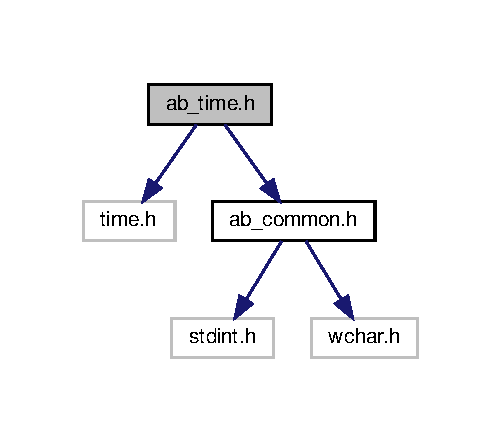
\includegraphics[width=241pt]{d7/d95/ab__time_8h__incl}
\end{center}
\end{figure}
This graph shows which files directly or indirectly include this file\+:\nopagebreak
\begin{figure}[H]
\begin{center}
\leavevmode
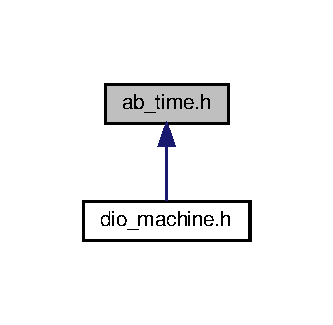
\includegraphics[width=160pt]{df/d0d/ab__time_8h__dep__incl}
\end{center}
\end{figure}
\subsection*{Typedefs}
\begin{DoxyCompactItemize}
\item 
typedef timespec \hyperlink{ab__time_8h_adc59735fd0d20e93fe3016c8b6a4f782}{abt\+\_\+time}
\end{DoxyCompactItemize}
\subsection*{Functions}
\begin{DoxyCompactItemize}
\item 
void \hyperlink{ab__time_8h_a55589396a22562f4037d2817a579e82e}{abt\+\_\+\+Get\+Current} (\hyperlink{ab__time_8h_adc59735fd0d20e93fe3016c8b6a4f782}{abt\+\_\+time} $\ast$Now)
\item 
\hyperlink{ab__time_8h_adc59735fd0d20e93fe3016c8b6a4f782}{abt\+\_\+time} \hyperlink{ab__time_8h_a410389a8363dbb7453520927331297d0}{abt\+\_\+\+Get\+Current} ()
\item 
\hyperlink{ab__time_8h_adc59735fd0d20e93fe3016c8b6a4f782}{abt\+\_\+time} \hyperlink{ab__time_8h_ad401e90e9886fe9e1fb5f49f2b11d8c0}{abt\+\_\+\+Get\+Monotonic} ()
\item 
\hyperlink{ab__common_8h_afaa62991928fb9fb18ff0db62a040aba}{u32} \hyperlink{ab__time_8h_ad3ab740dfcc9875efe4b1721fd374db4}{abt\+\_\+\+Get\+Elapsed\+Ms\+U32} (\hyperlink{ab__time_8h_adc59735fd0d20e93fe3016c8b6a4f782}{abt\+\_\+time} Start\+Time, \hyperlink{ab__time_8h_adc59735fd0d20e93fe3016c8b6a4f782}{abt\+\_\+time} Now)
\item 
\hyperlink{ab__common_8h_aafa04bc3cb166e826b75a23f4add4b59}{r32} \hyperlink{ab__time_8h_a9834c3b5b55da0fe4ae280550cf5d97f}{abt\+\_\+\+Get\+Elapsed\+Ms\+R32} (\hyperlink{ab__time_8h_adc59735fd0d20e93fe3016c8b6a4f782}{abt\+\_\+time} Start\+Time, \hyperlink{ab__time_8h_adc59735fd0d20e93fe3016c8b6a4f782}{abt\+\_\+time} Now)
\item 
\hyperlink{ab__time_8h_adc59735fd0d20e93fe3016c8b6a4f782}{abt\+\_\+time} \hyperlink{ab__time_8h_a126f380942c7e3e87802634893590928}{abt\+\_\+\+Get\+Wall\+Clock\+From\+Elapsed} (\hyperlink{ab__time_8h_adc59735fd0d20e93fe3016c8b6a4f782}{abt\+\_\+time} Start\+Time, \hyperlink{ab__common_8h_aafa04bc3cb166e826b75a23f4add4b59}{r32} Timestamp\+Ms)
\item 
\hyperlink{ab__common_8h_afaa62991928fb9fb18ff0db62a040aba}{u32} \hyperlink{ab__time_8h_ab8ae3038f353a3a59bc79abf35dcb4a4}{abt\+\_\+\+Get\+Ms\+From\+Time\+U32} (\hyperlink{ab__time_8h_adc59735fd0d20e93fe3016c8b6a4f782}{abt\+\_\+time} Time)
\item 
\hyperlink{ab__common_8h_afaa62991928fb9fb18ff0db62a040aba}{u32} \hyperlink{ab__time_8h_a05feba1d586786dad132d87c70acf336}{abt\+\_\+\+Get\+Ms\+From\+Time32} (\hyperlink{ab__time_8h_adc59735fd0d20e93fe3016c8b6a4f782}{abt\+\_\+time} Time)
\end{DoxyCompactItemize}


\subsection{Typedef Documentation}
\mbox{\Hypertarget{ab__time_8h_adc59735fd0d20e93fe3016c8b6a4f782}\label{ab__time_8h_adc59735fd0d20e93fe3016c8b6a4f782}} 
\index{ab\+\_\+time.\+h@{ab\+\_\+time.\+h}!abt\+\_\+time@{abt\+\_\+time}}
\index{abt\+\_\+time@{abt\+\_\+time}!ab\+\_\+time.\+h@{ab\+\_\+time.\+h}}
\subsubsection{\texorpdfstring{abt\+\_\+time}{abt\_time}}
{\footnotesize\ttfamily typedef timespec \hyperlink{ab__time_8h_adc59735fd0d20e93fe3016c8b6a4f782}{abt\+\_\+time}}



\subsection{Function Documentation}
\mbox{\Hypertarget{ab__time_8h_a55589396a22562f4037d2817a579e82e}\label{ab__time_8h_a55589396a22562f4037d2817a579e82e}} 
\index{ab\+\_\+time.\+h@{ab\+\_\+time.\+h}!abt\+\_\+\+Get\+Current@{abt\+\_\+\+Get\+Current}}
\index{abt\+\_\+\+Get\+Current@{abt\+\_\+\+Get\+Current}!ab\+\_\+time.\+h@{ab\+\_\+time.\+h}}
\subsubsection{\texorpdfstring{abt\+\_\+\+Get\+Current()}{abt\_GetCurrent()}\hspace{0.1cm}{\footnotesize\ttfamily [1/2]}}
{\footnotesize\ttfamily void abt\+\_\+\+Get\+Current (\begin{DoxyParamCaption}\item[{\hyperlink{ab__time_8h_adc59735fd0d20e93fe3016c8b6a4f782}{abt\+\_\+time} $\ast$}]{Now }\end{DoxyParamCaption})}

\mbox{\Hypertarget{ab__time_8h_a410389a8363dbb7453520927331297d0}\label{ab__time_8h_a410389a8363dbb7453520927331297d0}} 
\index{ab\+\_\+time.\+h@{ab\+\_\+time.\+h}!abt\+\_\+\+Get\+Current@{abt\+\_\+\+Get\+Current}}
\index{abt\+\_\+\+Get\+Current@{abt\+\_\+\+Get\+Current}!ab\+\_\+time.\+h@{ab\+\_\+time.\+h}}
\subsubsection{\texorpdfstring{abt\+\_\+\+Get\+Current()}{abt\_GetCurrent()}\hspace{0.1cm}{\footnotesize\ttfamily [2/2]}}
{\footnotesize\ttfamily \hyperlink{ab__time_8h_adc59735fd0d20e93fe3016c8b6a4f782}{abt\+\_\+time} abt\+\_\+\+Get\+Current (\begin{DoxyParamCaption}{ }\end{DoxyParamCaption})}

\mbox{\Hypertarget{ab__time_8h_a9834c3b5b55da0fe4ae280550cf5d97f}\label{ab__time_8h_a9834c3b5b55da0fe4ae280550cf5d97f}} 
\index{ab\+\_\+time.\+h@{ab\+\_\+time.\+h}!abt\+\_\+\+Get\+Elapsed\+Ms\+R32@{abt\+\_\+\+Get\+Elapsed\+Ms\+R32}}
\index{abt\+\_\+\+Get\+Elapsed\+Ms\+R32@{abt\+\_\+\+Get\+Elapsed\+Ms\+R32}!ab\+\_\+time.\+h@{ab\+\_\+time.\+h}}
\subsubsection{\texorpdfstring{abt\+\_\+\+Get\+Elapsed\+Ms\+R32()}{abt\_GetElapsedMsR32()}}
{\footnotesize\ttfamily \hyperlink{ab__common_8h_aafa04bc3cb166e826b75a23f4add4b59}{r32} abt\+\_\+\+Get\+Elapsed\+Ms\+R32 (\begin{DoxyParamCaption}\item[{\hyperlink{ab__time_8h_adc59735fd0d20e93fe3016c8b6a4f782}{abt\+\_\+time}}]{Start\+Time,  }\item[{\hyperlink{ab__time_8h_adc59735fd0d20e93fe3016c8b6a4f782}{abt\+\_\+time}}]{Now }\end{DoxyParamCaption})}

\mbox{\Hypertarget{ab__time_8h_ad3ab740dfcc9875efe4b1721fd374db4}\label{ab__time_8h_ad3ab740dfcc9875efe4b1721fd374db4}} 
\index{ab\+\_\+time.\+h@{ab\+\_\+time.\+h}!abt\+\_\+\+Get\+Elapsed\+Ms\+U32@{abt\+\_\+\+Get\+Elapsed\+Ms\+U32}}
\index{abt\+\_\+\+Get\+Elapsed\+Ms\+U32@{abt\+\_\+\+Get\+Elapsed\+Ms\+U32}!ab\+\_\+time.\+h@{ab\+\_\+time.\+h}}
\subsubsection{\texorpdfstring{abt\+\_\+\+Get\+Elapsed\+Ms\+U32()}{abt\_GetElapsedMsU32()}}
{\footnotesize\ttfamily \hyperlink{ab__common_8h_afaa62991928fb9fb18ff0db62a040aba}{u32} abt\+\_\+\+Get\+Elapsed\+Ms\+U32 (\begin{DoxyParamCaption}\item[{\hyperlink{ab__time_8h_adc59735fd0d20e93fe3016c8b6a4f782}{abt\+\_\+time}}]{Start\+Time,  }\item[{\hyperlink{ab__time_8h_adc59735fd0d20e93fe3016c8b6a4f782}{abt\+\_\+time}}]{Now }\end{DoxyParamCaption})}

\mbox{\Hypertarget{ab__time_8h_ad401e90e9886fe9e1fb5f49f2b11d8c0}\label{ab__time_8h_ad401e90e9886fe9e1fb5f49f2b11d8c0}} 
\index{ab\+\_\+time.\+h@{ab\+\_\+time.\+h}!abt\+\_\+\+Get\+Monotonic@{abt\+\_\+\+Get\+Monotonic}}
\index{abt\+\_\+\+Get\+Monotonic@{abt\+\_\+\+Get\+Monotonic}!ab\+\_\+time.\+h@{ab\+\_\+time.\+h}}
\subsubsection{\texorpdfstring{abt\+\_\+\+Get\+Monotonic()}{abt\_GetMonotonic()}}
{\footnotesize\ttfamily \hyperlink{ab__time_8h_adc59735fd0d20e93fe3016c8b6a4f782}{abt\+\_\+time} abt\+\_\+\+Get\+Monotonic (\begin{DoxyParamCaption}{ }\end{DoxyParamCaption})}

\mbox{\Hypertarget{ab__time_8h_a05feba1d586786dad132d87c70acf336}\label{ab__time_8h_a05feba1d586786dad132d87c70acf336}} 
\index{ab\+\_\+time.\+h@{ab\+\_\+time.\+h}!abt\+\_\+\+Get\+Ms\+From\+Time32@{abt\+\_\+\+Get\+Ms\+From\+Time32}}
\index{abt\+\_\+\+Get\+Ms\+From\+Time32@{abt\+\_\+\+Get\+Ms\+From\+Time32}!ab\+\_\+time.\+h@{ab\+\_\+time.\+h}}
\subsubsection{\texorpdfstring{abt\+\_\+\+Get\+Ms\+From\+Time32()}{abt\_GetMsFromTime32()}}
{\footnotesize\ttfamily \hyperlink{ab__common_8h_afaa62991928fb9fb18ff0db62a040aba}{u32} abt\+\_\+\+Get\+Ms\+From\+Time32 (\begin{DoxyParamCaption}\item[{\hyperlink{ab__time_8h_adc59735fd0d20e93fe3016c8b6a4f782}{abt\+\_\+time}}]{Time }\end{DoxyParamCaption})\hspace{0.3cm}{\ttfamily [inline]}}

\mbox{\Hypertarget{ab__time_8h_ab8ae3038f353a3a59bc79abf35dcb4a4}\label{ab__time_8h_ab8ae3038f353a3a59bc79abf35dcb4a4}} 
\index{ab\+\_\+time.\+h@{ab\+\_\+time.\+h}!abt\+\_\+\+Get\+Ms\+From\+Time\+U32@{abt\+\_\+\+Get\+Ms\+From\+Time\+U32}}
\index{abt\+\_\+\+Get\+Ms\+From\+Time\+U32@{abt\+\_\+\+Get\+Ms\+From\+Time\+U32}!ab\+\_\+time.\+h@{ab\+\_\+time.\+h}}
\subsubsection{\texorpdfstring{abt\+\_\+\+Get\+Ms\+From\+Time\+U32()}{abt\_GetMsFromTimeU32()}}
{\footnotesize\ttfamily \hyperlink{ab__common_8h_afaa62991928fb9fb18ff0db62a040aba}{u32} abt\+\_\+\+Get\+Ms\+From\+Time\+U32 (\begin{DoxyParamCaption}\item[{\hyperlink{ab__time_8h_adc59735fd0d20e93fe3016c8b6a4f782}{abt\+\_\+time}}]{Time }\end{DoxyParamCaption})\hspace{0.3cm}{\ttfamily [inline]}}

\mbox{\Hypertarget{ab__time_8h_a126f380942c7e3e87802634893590928}\label{ab__time_8h_a126f380942c7e3e87802634893590928}} 
\index{ab\+\_\+time.\+h@{ab\+\_\+time.\+h}!abt\+\_\+\+Get\+Wall\+Clock\+From\+Elapsed@{abt\+\_\+\+Get\+Wall\+Clock\+From\+Elapsed}}
\index{abt\+\_\+\+Get\+Wall\+Clock\+From\+Elapsed@{abt\+\_\+\+Get\+Wall\+Clock\+From\+Elapsed}!ab\+\_\+time.\+h@{ab\+\_\+time.\+h}}
\subsubsection{\texorpdfstring{abt\+\_\+\+Get\+Wall\+Clock\+From\+Elapsed()}{abt\_GetWallClockFromElapsed()}}
{\footnotesize\ttfamily \hyperlink{ab__time_8h_adc59735fd0d20e93fe3016c8b6a4f782}{abt\+\_\+time} abt\+\_\+\+Get\+Wall\+Clock\+From\+Elapsed (\begin{DoxyParamCaption}\item[{\hyperlink{ab__time_8h_adc59735fd0d20e93fe3016c8b6a4f782}{abt\+\_\+time}}]{Start\+Time,  }\item[{\hyperlink{ab__common_8h_aafa04bc3cb166e826b75a23f4add4b59}{r32}}]{Timestamp\+Ms }\end{DoxyParamCaption})}


\hypertarget{abp__enums_8cpp}{}\section{abp\+\_\+enums.\+cpp File Reference}
\label{abp__enums_8cpp}\index{abp\+\_\+enums.\+cpp@{abp\+\_\+enums.\+cpp}}


Enum Class Tags.  


{\ttfamily \#include \char`\"{}ab\+\_\+parser.\+h\char`\"{}}\newline
{\ttfamily \#include \char`\"{}ab\+\_\+lexer.\+h\char`\"{}}\newline
Include dependency graph for abp\+\_\+enums.\+cpp\+:
\nopagebreak
\begin{figure}[H]
\begin{center}
\leavevmode
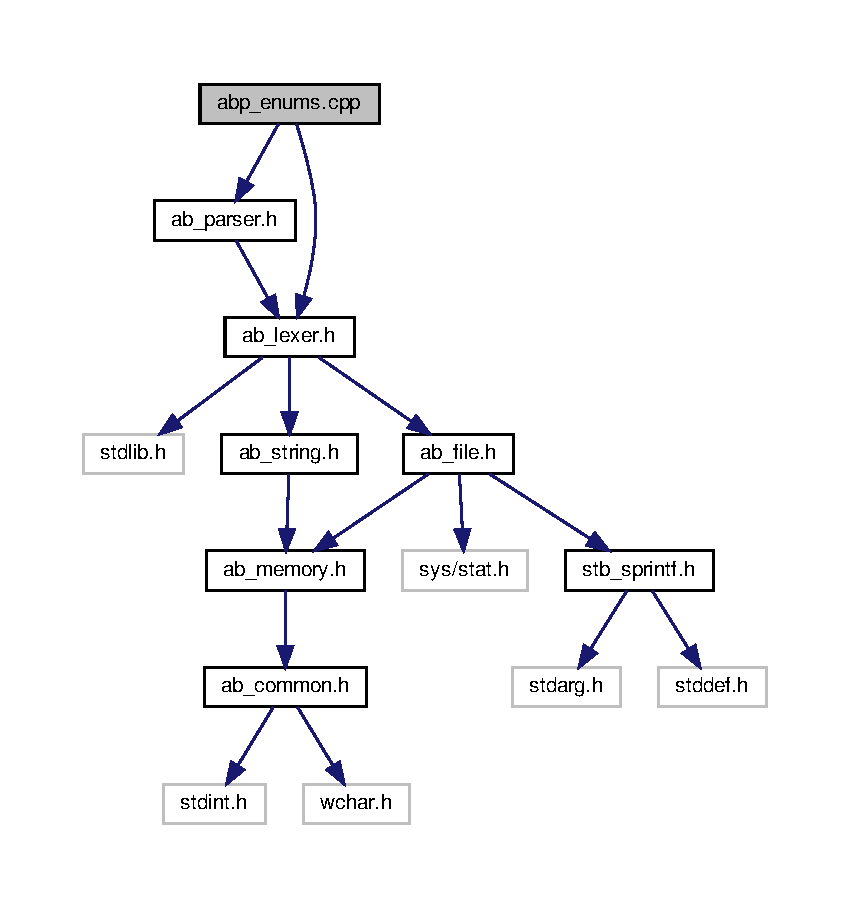
\includegraphics[width=283pt]{da/d42/abp__enums_8cpp__incl}
\end{center}
\end{figure}
This graph shows which files directly or indirectly include this file\+:
\nopagebreak
\begin{figure}[H]
\begin{center}
\leavevmode
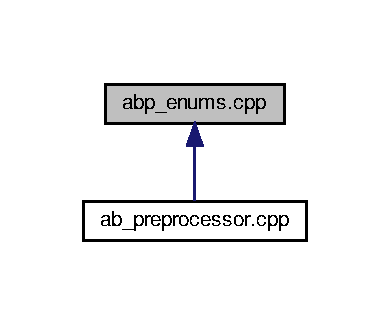
\includegraphics[width=187pt]{d9/d12/abp__enums_8cpp__dep__incl}
\end{center}
\end{figure}
\subsection*{Functions}
\begin{DoxyCompactItemize}
\item 
void \hyperlink{abp__enums_8cpp_a26413cc98eb64d610cf9f604afeb08c0}{Create\+Enum\+Json} (\hyperlink{structterm__enum}{term\+\_\+enum} $\ast$Enum, \hyperlink{structtag}{tag} $\ast$Tag, memory\+\_\+arena $\ast$Memory, \hyperlink{structoutput__data}{output\+\_\+data} $\ast$Definitions\+Out, \hyperlink{structoutput__data}{output\+\_\+data} $\ast$Functions\+Out)
\begin{DoxyCompactList}\small\item\em J\+S\+ON tag processing. \end{DoxyCompactList}\item 
void \hyperlink{abp__enums_8cpp_a4074cdfd980dd68492498531fae10c24}{Create\+Enum\+Labels} (\hyperlink{structterm__enum}{term\+\_\+enum} $\ast$Enum, \hyperlink{structtag}{tag} $\ast$Label\+Tag, memory\+\_\+arena $\ast$Memory, \hyperlink{structoutput__data}{output\+\_\+data} $\ast$Definitions\+Out, \hyperlink{structoutput__data}{output\+\_\+data} $\ast$Functions\+Out)
\begin{DoxyCompactList}\small\item\em Enum Label processing. \end{DoxyCompactList}\item 
void \hyperlink{abp__enums_8cpp_a06ef0f7fc80dcb43ccd2f3e040a30965}{Create\+Enum\+Strings} (\hyperlink{structterm__enum}{term\+\_\+enum} $\ast$Enum, \hyperlink{structtag}{tag} $\ast$Tag, memory\+\_\+arena $\ast$Memory, \hyperlink{structoutput__data}{output\+\_\+data} $\ast$Definitions\+Out, \hyperlink{structoutput__data}{output\+\_\+data} $\ast$Functions\+Out)
\begin{DoxyCompactList}\small\item\em Enum Strings T\+AG processing. \end{DoxyCompactList}\item 
void \hyperlink{abp__enums_8cpp_a9de7ea142237a33f158a301d823bfe35}{Process\+Enums} (\hyperlink{structterm__enum}{term\+\_\+enum} $\ast$Enum\+List\+Sentinal, memory\+\_\+arena $\ast$Memory, \hyperlink{structoutput__data}{output\+\_\+data} $\ast$Headers, \hyperlink{structoutput__data}{output\+\_\+data} $\ast$Definitions)
\begin{DoxyCompactList}\small\item\em Process all enums. \end{DoxyCompactList}\end{DoxyCompactItemize}


\subsection{Detailed Description}
Enum Class Tags. 

\begin{DoxyAuthor}{Author}
Amos Buchanan 
\end{DoxyAuthor}
\begin{DoxyVersion}{Version}
1.\+0 
\end{DoxyVersion}
\begin{DoxyDate}{Date}
2020 
\end{DoxyDate}
\begin{DoxyCopyright}{Copyright}
\href{https://opensource.org/licenses/MIT}{\tt M\+IT Public License}
\end{DoxyCopyright}
This is the source file for the tags used in enum class. All enum class tag definitions go here. There are no tags for C-\/style enums; any C-\/style enums with a \hyperlink{PreprocTest_8h_a2606cd56d2d8f567785bde5848176722}{T\+A\+G()} will be ignored.

See the \hyperlink{index}{Readme.md} file for more information on usage.

To add a new tag\+:
\begin{DoxyItemize}
\item Write a function to create the header and function portion of the enums.
\item Update the \hyperlink{abp__enums_8cpp_a9de7ea142237a33f158a301d823bfe35}{Process\+Enums} function with the tag and new function.
\end{DoxyItemize}\hypertarget{abp__enums_8cpp_autotoc_md1}{}\subsection{M\+I\+T License}\label{abp__enums_8cpp_autotoc_md1}
\href{https://opensource.org/licenses/MIT}{\tt https\+://opensource.\+org/licenses/\+M\+IT}

Copyright 2020 Amos Buchanan

Permission is hereby granted, free of charge, to any person obtaining a copy of this software and associated documentation files (the \char`\"{}\+Software\char`\"{}), to deal in the Software without restriction, including without limitation the rights to use, copy, modify, merge, publish, distribute, sublicense, and/or sell copies of the Software, and to permit persons to whom the Software is furnished to do so, subject to the following conditions\+:

The above copyright notice and this permission notice shall be included in all copies or substantial portions of the Software.

T\+HE S\+O\+F\+T\+W\+A\+RE IS P\+R\+O\+V\+I\+D\+ED \char`\"{}\+A\+S I\+S\char`\"{}, W\+I\+T\+H\+O\+UT W\+A\+R\+R\+A\+N\+TY OF A\+NY K\+I\+ND, E\+X\+P\+R\+E\+SS OR I\+M\+P\+L\+I\+ED, I\+N\+C\+L\+U\+D\+I\+NG B\+UT N\+OT L\+I\+M\+I\+T\+ED TO T\+HE W\+A\+R\+R\+A\+N\+T\+I\+ES OF M\+E\+R\+C\+H\+A\+N\+T\+A\+B\+I\+L\+I\+TY, F\+I\+T\+N\+E\+SS F\+OR A P\+A\+R\+T\+I\+C\+U\+L\+AR P\+U\+R\+P\+O\+SE A\+ND N\+O\+N\+I\+N\+F\+R\+I\+N\+G\+E\+M\+E\+NT. IN NO E\+V\+E\+NT S\+H\+A\+LL T\+HE A\+U\+T\+H\+O\+RS OR C\+O\+P\+Y\+R\+I\+G\+HT H\+O\+L\+D\+E\+RS BE L\+I\+A\+B\+LE F\+OR A\+NY C\+L\+A\+IM, D\+A\+M\+A\+G\+ES OR O\+T\+H\+ER L\+I\+A\+B\+I\+L\+I\+TY, W\+H\+E\+T\+H\+ER IN AN A\+C\+T\+I\+ON OF C\+O\+N\+T\+R\+A\+CT, T\+O\+RT OR O\+T\+H\+E\+R\+W\+I\+SE, A\+R\+I\+S\+I\+NG F\+R\+OM, O\+UT OF OR IN C\+O\+N\+N\+E\+C\+T\+I\+ON W\+I\+TH T\+HE S\+O\+F\+T\+W\+A\+RE OR T\+HE U\+SE OR O\+T\+H\+ER D\+E\+A\+L\+I\+N\+GS IN T\+HE S\+O\+F\+T\+W\+A\+RE. 

\subsection{Function Documentation}
\mbox{\Hypertarget{abp__enums_8cpp_a26413cc98eb64d610cf9f604afeb08c0}\label{abp__enums_8cpp_a26413cc98eb64d610cf9f604afeb08c0}} 
\index{abp\+\_\+enums.\+cpp@{abp\+\_\+enums.\+cpp}!Create\+Enum\+Json@{Create\+Enum\+Json}}
\index{Create\+Enum\+Json@{Create\+Enum\+Json}!abp\+\_\+enums.\+cpp@{abp\+\_\+enums.\+cpp}}
\subsubsection{\texorpdfstring{Create\+Enum\+Json()}{CreateEnumJson()}}
{\footnotesize\ttfamily void Create\+Enum\+Json (\begin{DoxyParamCaption}\item[{\hyperlink{structterm__enum}{term\+\_\+enum} $\ast$}]{Enum,  }\item[{\hyperlink{structtag}{tag} $\ast$}]{Tag,  }\item[{memory\+\_\+arena $\ast$}]{Memory,  }\item[{\hyperlink{structoutput__data}{output\+\_\+data} $\ast$}]{Definitions\+Out,  }\item[{\hyperlink{structoutput__data}{output\+\_\+data} $\ast$}]{Functions\+Out }\end{DoxyParamCaption})}



J\+S\+ON tag processing. 

This function processes the J\+S\+ON tag. Usage\+:


\begin{DoxyCode}
\hyperlink{PreprocTest_8h_a2606cd56d2d8f567785bde5848176722}{TAG}(JSON);
\textcolor{keyword}{enum class} SomeEnum
\{
 One,
 Two,
 Three
\};
\end{DoxyCode}
 \mbox{\Hypertarget{abp__enums_8cpp_a4074cdfd980dd68492498531fae10c24}\label{abp__enums_8cpp_a4074cdfd980dd68492498531fae10c24}} 
\index{abp\+\_\+enums.\+cpp@{abp\+\_\+enums.\+cpp}!Create\+Enum\+Labels@{Create\+Enum\+Labels}}
\index{Create\+Enum\+Labels@{Create\+Enum\+Labels}!abp\+\_\+enums.\+cpp@{abp\+\_\+enums.\+cpp}}
\subsubsection{\texorpdfstring{Create\+Enum\+Labels()}{CreateEnumLabels()}}
{\footnotesize\ttfamily void Create\+Enum\+Labels (\begin{DoxyParamCaption}\item[{\hyperlink{structterm__enum}{term\+\_\+enum} $\ast$}]{Enum,  }\item[{\hyperlink{structtag}{tag} $\ast$}]{Label\+Tag,  }\item[{memory\+\_\+arena $\ast$}]{Memory,  }\item[{\hyperlink{structoutput__data}{output\+\_\+data} $\ast$}]{Definitions\+Out,  }\item[{\hyperlink{structoutput__data}{output\+\_\+data} $\ast$}]{Functions\+Out }\end{DoxyParamCaption})}



Enum Label processing. 

This function processes enums for the Label tag.

Usage\+:


\begin{DoxyCode}
\hyperlink{PreprocTest_8h_a2606cd56d2d8f567785bde5848176722}{TAG}(Label:Number);
\textcolor{keyword}{enum class} SomeEnum
\{
\hyperlink{PreprocTest_8h_a2606cd56d2d8f567785bde5848176722}{TAG}(Number:\textcolor{stringliteral}{"1 - One"})
 One,
\hyperlink{PreprocTest_8h_a2606cd56d2d8f567785bde5848176722}{TAG}(Number:\textcolor{stringliteral}{"2 - Two"})
 Two,
\hyperlink{PreprocTest_8h_a2606cd56d2d8f567785bde5848176722}{TAG}(Number:\textcolor{stringliteral}{"3 - Three"})
 Three
\};
\end{DoxyCode}
 \mbox{\Hypertarget{abp__enums_8cpp_a06ef0f7fc80dcb43ccd2f3e040a30965}\label{abp__enums_8cpp_a06ef0f7fc80dcb43ccd2f3e040a30965}} 
\index{abp\+\_\+enums.\+cpp@{abp\+\_\+enums.\+cpp}!Create\+Enum\+Strings@{Create\+Enum\+Strings}}
\index{Create\+Enum\+Strings@{Create\+Enum\+Strings}!abp\+\_\+enums.\+cpp@{abp\+\_\+enums.\+cpp}}
\subsubsection{\texorpdfstring{Create\+Enum\+Strings()}{CreateEnumStrings()}}
{\footnotesize\ttfamily void Create\+Enum\+Strings (\begin{DoxyParamCaption}\item[{\hyperlink{structterm__enum}{term\+\_\+enum} $\ast$}]{Enum,  }\item[{\hyperlink{structtag}{tag} $\ast$}]{Tag,  }\item[{memory\+\_\+arena $\ast$}]{Memory,  }\item[{\hyperlink{structoutput__data}{output\+\_\+data} $\ast$}]{Definitions\+Out,  }\item[{\hyperlink{structoutput__data}{output\+\_\+data} $\ast$}]{Functions\+Out }\end{DoxyParamCaption})}



Enum Strings T\+AG processing. 

This function processes enums for the Strings tag.

Usage\+:


\begin{DoxyCode}
\hyperlink{PreprocTest_8h_a2606cd56d2d8f567785bde5848176722}{TAG}(Strings);
\textcolor{keyword}{enum class} SomeEnum
\{
 Unknown,
 One,
 Two,
 Three
\};
\end{DoxyCode}
 \mbox{\Hypertarget{abp__enums_8cpp_a9de7ea142237a33f158a301d823bfe35}\label{abp__enums_8cpp_a9de7ea142237a33f158a301d823bfe35}} 
\index{abp\+\_\+enums.\+cpp@{abp\+\_\+enums.\+cpp}!Process\+Enums@{Process\+Enums}}
\index{Process\+Enums@{Process\+Enums}!abp\+\_\+enums.\+cpp@{abp\+\_\+enums.\+cpp}}
\subsubsection{\texorpdfstring{Process\+Enums()}{ProcessEnums()}}
{\footnotesize\ttfamily void Process\+Enums (\begin{DoxyParamCaption}\item[{\hyperlink{structterm__enum}{term\+\_\+enum} $\ast$}]{Enum\+List\+Sentinal,  }\item[{memory\+\_\+arena $\ast$}]{Memory,  }\item[{\hyperlink{structoutput__data}{output\+\_\+data} $\ast$}]{Headers,  }\item[{\hyperlink{structoutput__data}{output\+\_\+data} $\ast$}]{Definitions }\end{DoxyParamCaption})}



Process all enums. 

Process all of the tags in the enums. This calls out to the individual functions for each tag. 
\hypertarget{abp__queue_8cpp}{}\doxysection{abp\+\_\+queue.\+cpp File Reference}
\label{abp__queue_8cpp}\index{abp\_queue.cpp@{abp\_queue.cpp}}
\doxysubsection*{Functions}
\begin{DoxyCompactItemize}
\item 
void \mbox{\hyperlink{abp__queue_8cpp_adf5d415a788af605e6b18d0d67385dae}{Write\+Queue\+Functions\+Queue}} (ads\+\_\+stringptr Queue\+Item\+Name, u32 Queue\+Size, memory\+\_\+arena $\ast$Memory, \mbox{\hyperlink{structoutput__data}{output\+\_\+data}} $\ast$Headers, \mbox{\hyperlink{structoutput__data}{output\+\_\+data}} $\ast$Definitions)
\end{DoxyCompactItemize}


\doxysubsection{Function Documentation}
\mbox{\Hypertarget{abp__queue_8cpp_adf5d415a788af605e6b18d0d67385dae}\label{abp__queue_8cpp_adf5d415a788af605e6b18d0d67385dae}} 
\index{abp\_queue.cpp@{abp\_queue.cpp}!WriteQueueFunctionsQueue@{WriteQueueFunctionsQueue}}
\index{WriteQueueFunctionsQueue@{WriteQueueFunctionsQueue}!abp\_queue.cpp@{abp\_queue.cpp}}
\doxysubsubsection{\texorpdfstring{WriteQueueFunctionsQueue()}{WriteQueueFunctionsQueue()}}
{\footnotesize\ttfamily void Write\+Queue\+Functions\+Queue (\begin{DoxyParamCaption}\item[{ads\+\_\+stringptr}]{Queue\+Item\+Name,  }\item[{u32}]{Queue\+Size,  }\item[{memory\+\_\+arena $\ast$}]{Memory,  }\item[{\mbox{\hyperlink{structoutput__data}{output\+\_\+data}} $\ast$}]{Headers,  }\item[{\mbox{\hyperlink{structoutput__data}{output\+\_\+data}} $\ast$}]{Definitions }\end{DoxyParamCaption})}


\hypertarget{abp__queue_8h}{}\doxysection{abp\+\_\+queue.\+h File Reference}
\label{abp__queue_8h}\index{abp\_queue.h@{abp\_queue.h}}
{\ttfamily \#include \char`\"{}ab\+\_\+string.\+h\char`\"{}}\newline
{\ttfamily \#include \char`\"{}ab\+\_\+parser.\+h\char`\"{}}\newline
Include dependency graph for abp\+\_\+queue.\+h\+:\nopagebreak
\begin{figure}[H]
\begin{center}
\leavevmode
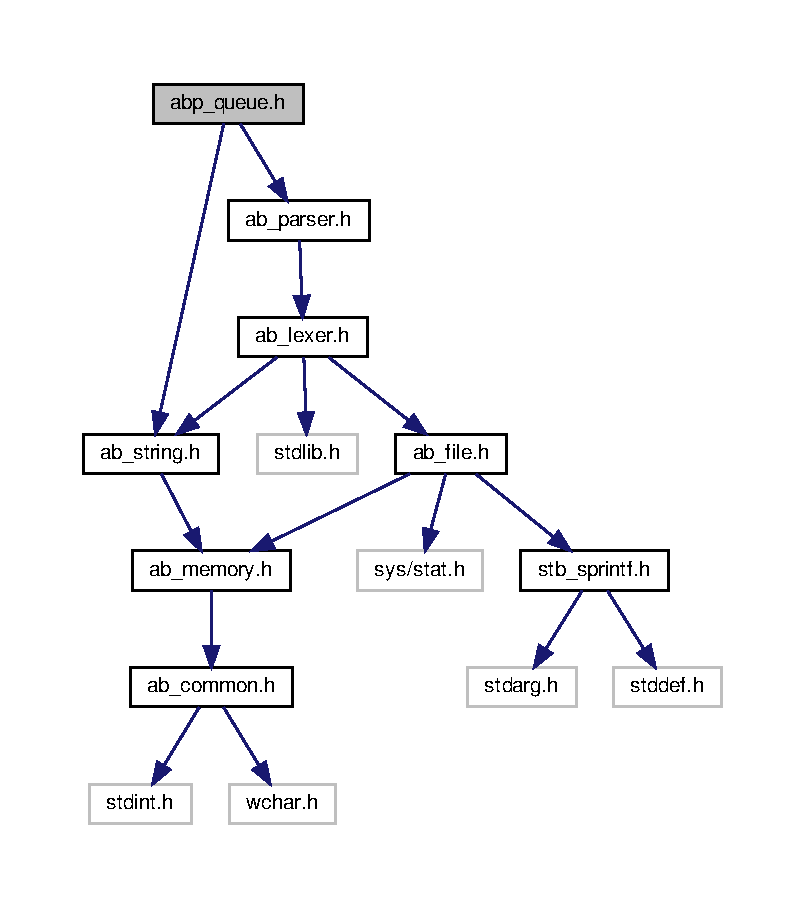
\includegraphics[width=350pt]{d6/d00/abp__queue_8h__incl}
\end{center}
\end{figure}
This graph shows which files directly or indirectly include this file\+:\nopagebreak
\begin{figure}[H]
\begin{center}
\leavevmode
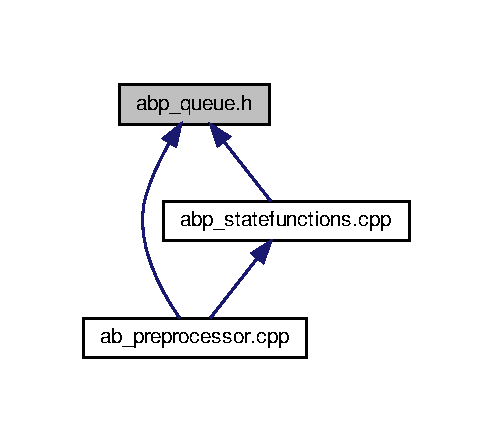
\includegraphics[width=237pt]{d6/dc7/abp__queue_8h__dep__incl}
\end{center}
\end{figure}
\doxysubsection*{Functions}
\begin{DoxyCompactItemize}
\item 
void \mbox{\hyperlink{abp__queue_8h_af0c59e83e14269261deebc96560ee1bb}{Write\+Queue\+Functions}} (abs\+\_\+stringptr Queue\+Item\+Name, u32 Queue\+Size, memory\+\_\+arena $\ast$Memory, \mbox{\hyperlink{structoutput__data}{output\+\_\+data}} $\ast$Headers, \mbox{\hyperlink{structoutput__data}{output\+\_\+data}} $\ast$Definitions)
\end{DoxyCompactItemize}


\doxysubsection{Function Documentation}
\mbox{\Hypertarget{abp__queue_8h_af0c59e83e14269261deebc96560ee1bb}\label{abp__queue_8h_af0c59e83e14269261deebc96560ee1bb}} 
\index{abp\_queue.h@{abp\_queue.h}!WriteQueueFunctions@{WriteQueueFunctions}}
\index{WriteQueueFunctions@{WriteQueueFunctions}!abp\_queue.h@{abp\_queue.h}}
\doxysubsubsection{\texorpdfstring{WriteQueueFunctions()}{WriteQueueFunctions()}}
{\footnotesize\ttfamily void Write\+Queue\+Functions (\begin{DoxyParamCaption}\item[{abs\+\_\+stringptr}]{Queue\+Item\+Name,  }\item[{u32}]{Queue\+Size,  }\item[{memory\+\_\+arena $\ast$}]{Memory,  }\item[{\mbox{\hyperlink{structoutput__data}{output\+\_\+data}} $\ast$}]{Headers,  }\item[{\mbox{\hyperlink{structoutput__data}{output\+\_\+data}} $\ast$}]{Definitions }\end{DoxyParamCaption})}


\hypertarget{abp__statefunctions_8cpp}{}\section{abp\+\_\+statefunctions.\+cpp File Reference}
\label{abp__statefunctions_8cpp}\index{abp\+\_\+statefunctions.\+cpp@{abp\+\_\+statefunctions.\+cpp}}
{\ttfamily \#include \char`\"{}abp\+\_\+queue.\+h\char`\"{}}\newline
Include dependency graph for abp\+\_\+statefunctions.\+cpp\+:\nopagebreak
\begin{figure}[H]
\begin{center}
\leavevmode
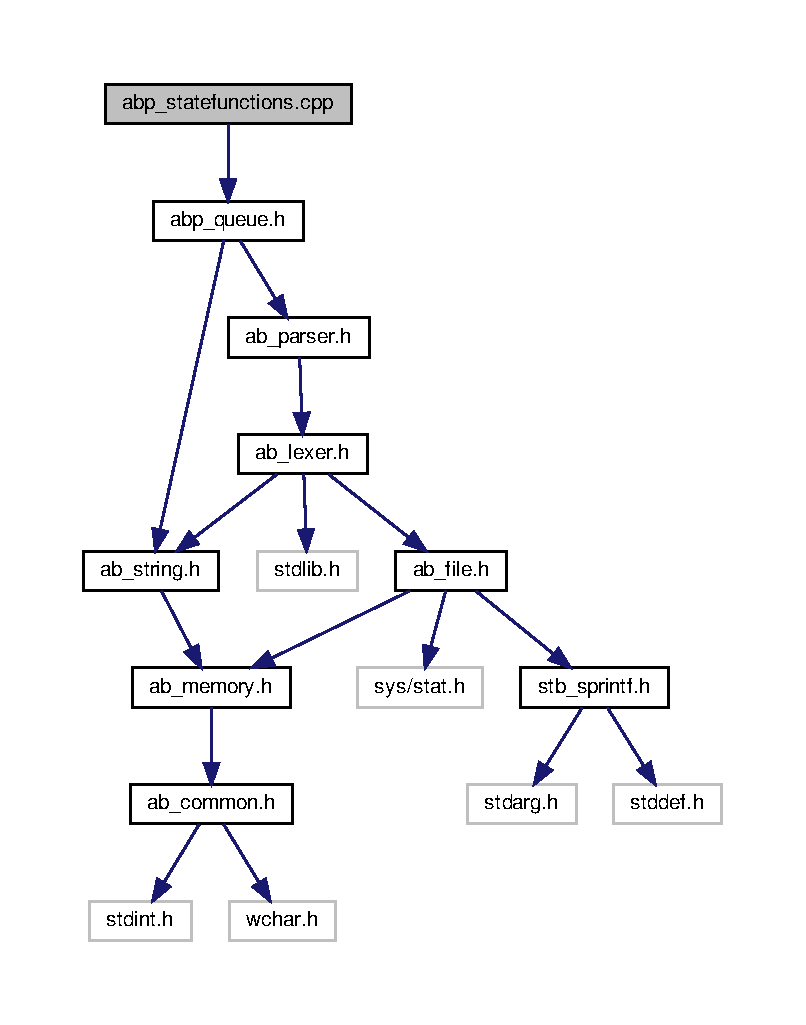
\includegraphics[width=350pt]{dc/dbe/abp__statefunctions_8cpp__incl}
\end{center}
\end{figure}
This graph shows which files directly or indirectly include this file\+:\nopagebreak
\begin{figure}[H]
\begin{center}
\leavevmode
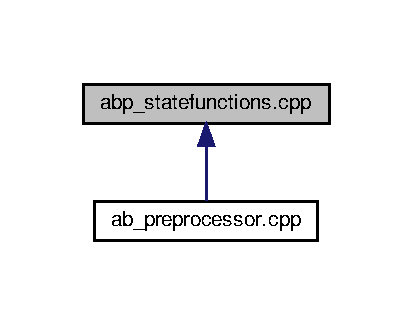
\includegraphics[width=198pt]{da/dac/abp__statefunctions_8cpp__dep__incl}
\end{center}
\end{figure}
\subsection*{Functions}
\begin{DoxyCompactItemize}
\item 
void \hyperlink{abp__statefunctions_8cpp_a26d1e099fd560e842eeb4ab5c9a39e87}{Process\+State\+Functions} (\hyperlink{structterm__statemachine}{term\+\_\+statemachine} $\ast$Machine\+List\+Sentinal, \hyperlink{structterm__definedfunction}{term\+\_\+definedfunction} $\ast$Defined\+Function\+List\+Sentinal, \hyperlink{structmemory__arena}{memory\+\_\+arena} $\ast$Memory, \hyperlink{structoutput__data}{output\+\_\+data} $\ast$Headers, \hyperlink{structoutput__data}{output\+\_\+data} $\ast$Definitions)
\end{DoxyCompactItemize}


\subsection{Function Documentation}
\mbox{\Hypertarget{abp__statefunctions_8cpp_a26d1e099fd560e842eeb4ab5c9a39e87}\label{abp__statefunctions_8cpp_a26d1e099fd560e842eeb4ab5c9a39e87}} 
\index{abp\+\_\+statefunctions.\+cpp@{abp\+\_\+statefunctions.\+cpp}!Process\+State\+Functions@{Process\+State\+Functions}}
\index{Process\+State\+Functions@{Process\+State\+Functions}!abp\+\_\+statefunctions.\+cpp@{abp\+\_\+statefunctions.\+cpp}}
\subsubsection{\texorpdfstring{Process\+State\+Functions()}{ProcessStateFunctions()}}
{\footnotesize\ttfamily void Process\+State\+Functions (\begin{DoxyParamCaption}\item[{\hyperlink{structterm__statemachine}{term\+\_\+statemachine} $\ast$}]{Machine\+List\+Sentinal,  }\item[{\hyperlink{structterm__definedfunction}{term\+\_\+definedfunction} $\ast$}]{Defined\+Function\+List\+Sentinal,  }\item[{\hyperlink{structmemory__arena}{memory\+\_\+arena} $\ast$}]{Memory,  }\item[{\hyperlink{structoutput__data}{output\+\_\+data} $\ast$}]{Headers,  }\item[{\hyperlink{structoutput__data}{output\+\_\+data} $\ast$}]{Definitions }\end{DoxyParamCaption})}


\hypertarget{abp__structs_8cpp}{}\doxysection{abp\+\_\+structs.\+cpp File Reference}
\label{abp__structs_8cpp}\index{abp\_structs.cpp@{abp\_structs.cpp}}


Struct/\+Union Class Tags.  


{\ttfamily \#include \char`\"{}ab\+\_\+string.\+h\char`\"{}}\newline
{\ttfamily \#include \char`\"{}ab\+\_\+memory.\+h\char`\"{}}\newline
{\ttfamily \#include \char`\"{}stb\+\_\+sprintf.\+h\char`\"{}}\newline
Include dependency graph for abp\+\_\+structs.\+cpp\+:\nopagebreak
\begin{figure}[H]
\begin{center}
\leavevmode
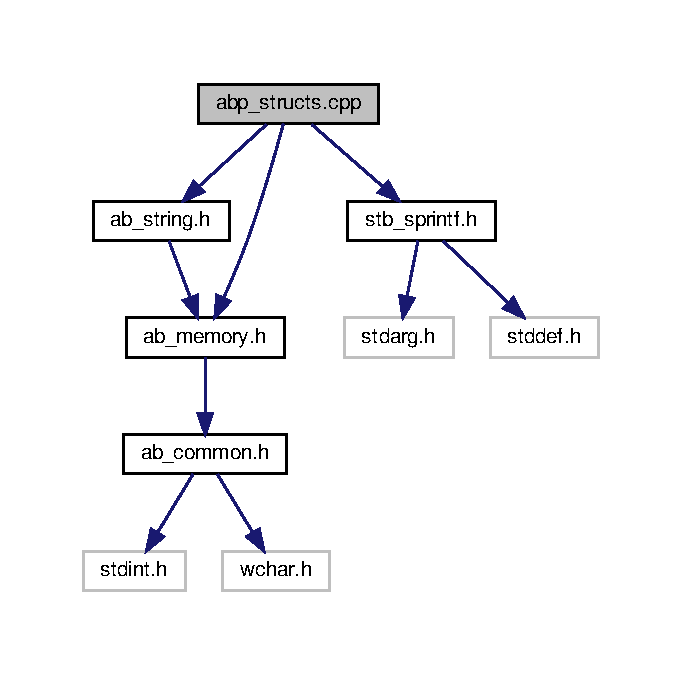
\includegraphics[width=329pt]{db/d79/abp__structs_8cpp__incl}
\end{center}
\end{figure}
This graph shows which files directly or indirectly include this file\+:\nopagebreak
\begin{figure}[H]
\begin{center}
\leavevmode
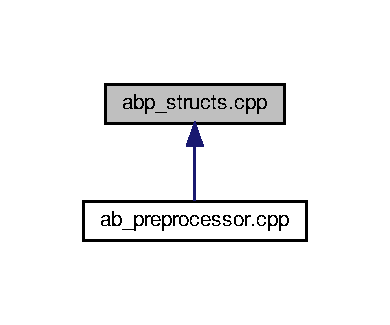
\includegraphics[width=187pt]{d8/d8f/abp__structs_8cpp__dep__incl}
\end{center}
\end{figure}
\doxysubsection*{Functions}
\begin{DoxyCompactItemize}
\item 
void \mbox{\hyperlink{abp__structs_8cpp_a9d82f4e668411580de7952f3c0089336}{Create\+Struct\+Json}} (\mbox{\hyperlink{structterm__struct}{term\+\_\+struct}} $\ast$Struct, \mbox{\hyperlink{structtag}{tag}} $\ast$Tag, memory\+\_\+arena $\ast$Memory, \mbox{\hyperlink{structoutput__data}{output\+\_\+data}} $\ast$Headers, \mbox{\hyperlink{structoutput__data}{output\+\_\+data}} $\ast$Definitions)
\begin{DoxyCompactList}\small\item\em J\+S\+ON tag processing. \end{DoxyCompactList}\item 
void \mbox{\hyperlink{abp__structs_8cpp_a0c8c66e0c511338fa2b1df03d78a52ae}{Process\+Structs}} (\mbox{\hyperlink{structterm__struct}{term\+\_\+struct}} $\ast$Struct\+List\+Sentinal, memory\+\_\+arena $\ast$Memory, \mbox{\hyperlink{structoutput__data}{output\+\_\+data}} $\ast$Headers, \mbox{\hyperlink{structoutput__data}{output\+\_\+data}} $\ast$Definitions)
\begin{DoxyCompactList}\small\item\em Handle the tags and call the struct create functions. \end{DoxyCompactList}\end{DoxyCompactItemize}


\doxysubsection{Detailed Description}
Struct/\+Union Class Tags. 

\begin{DoxyAuthor}{Author}
Amos Buchanan 
\end{DoxyAuthor}
\begin{DoxyVersion}{Version}
1.\+0 
\end{DoxyVersion}
\begin{DoxyDate}{Date}
2020 
\end{DoxyDate}
\begin{DoxyCopyright}{Copyright}
\href{https://opensource.org/licenses/MIT}{\texttt{ M\+IT Public License}}
\end{DoxyCopyright}
This is the source file for the tags used in structs and unions. All struct/union tag definitions go here. There is no difference between struct and union for this purpose.

See the \mbox{\hyperlink{index}{Readme.md}} file for more information on usage.

To add a new tag\+:
\begin{DoxyItemize}
\item Write a function to create the header and function portion of the struct functions and definitions..
\item Update the \mbox{\hyperlink{abp__structs_8cpp_a0c8c66e0c511338fa2b1df03d78a52ae}{Process\+Structs}} function with the tag and new function.
\end{DoxyItemize}\hypertarget{abp__structs_8cpp_autotoc_md4}{}\doxysubsection{M\+I\+T License}\label{abp__structs_8cpp_autotoc_md4}
\href{https://opensource.org/licenses/MIT}{\texttt{ https\+://opensource.\+org/licenses/\+M\+IT}}

Copyright 2020 Amos Buchanan

Permission is hereby granted, free of charge, to any person obtaining a copy of this software and associated documentation files (the \char`\"{}\+Software\char`\"{}), to deal in the Software without restriction, including without limitation the rights to use, copy, modify, merge, publish, distribute, sublicense, and/or sell copies of the Software, and to permit persons to whom the Software is furnished to do so, subject to the following conditions\+:

The above copyright notice and this permission notice shall be included in all copies or substantial portions of the Software.

T\+HE S\+O\+F\+T\+W\+A\+RE IS P\+R\+O\+V\+I\+D\+ED \char`\"{}\+A\+S I\+S\char`\"{}, W\+I\+T\+H\+O\+UT W\+A\+R\+R\+A\+N\+TY OF A\+NY K\+I\+ND, E\+X\+P\+R\+E\+SS OR I\+M\+P\+L\+I\+ED, I\+N\+C\+L\+U\+D\+I\+NG B\+UT N\+OT L\+I\+M\+I\+T\+ED TO T\+HE W\+A\+R\+R\+A\+N\+T\+I\+ES OF M\+E\+R\+C\+H\+A\+N\+T\+A\+B\+I\+L\+I\+TY, F\+I\+T\+N\+E\+SS F\+OR A P\+A\+R\+T\+I\+C\+U\+L\+AR P\+U\+R\+P\+O\+SE A\+ND N\+O\+N\+I\+N\+F\+R\+I\+N\+G\+E\+M\+E\+NT. IN NO E\+V\+E\+NT S\+H\+A\+LL T\+HE A\+U\+T\+H\+O\+RS OR C\+O\+P\+Y\+R\+I\+G\+HT H\+O\+L\+D\+E\+RS BE L\+I\+A\+B\+LE F\+OR A\+NY C\+L\+A\+IM, D\+A\+M\+A\+G\+ES OR O\+T\+H\+ER L\+I\+A\+B\+I\+L\+I\+TY, W\+H\+E\+T\+H\+ER IN AN A\+C\+T\+I\+ON OF C\+O\+N\+T\+R\+A\+CT, T\+O\+RT OR O\+T\+H\+E\+R\+W\+I\+SE, A\+R\+I\+S\+I\+NG F\+R\+OM, O\+UT OF OR IN C\+O\+N\+N\+E\+C\+T\+I\+ON W\+I\+TH T\+HE S\+O\+F\+T\+W\+A\+RE OR T\+HE U\+SE OR O\+T\+H\+ER D\+E\+A\+L\+I\+N\+GS IN T\+HE S\+O\+F\+T\+W\+A\+RE. 

\doxysubsection{Function Documentation}
\mbox{\Hypertarget{abp__structs_8cpp_a9d82f4e668411580de7952f3c0089336}\label{abp__structs_8cpp_a9d82f4e668411580de7952f3c0089336}} 
\index{abp\_structs.cpp@{abp\_structs.cpp}!CreateStructJson@{CreateStructJson}}
\index{CreateStructJson@{CreateStructJson}!abp\_structs.cpp@{abp\_structs.cpp}}
\doxysubsubsection{\texorpdfstring{CreateStructJson()}{CreateStructJson()}}
{\footnotesize\ttfamily void Create\+Struct\+Json (\begin{DoxyParamCaption}\item[{\mbox{\hyperlink{structterm__struct}{term\+\_\+struct}} $\ast$}]{Struct,  }\item[{\mbox{\hyperlink{structtag}{tag}} $\ast$}]{Tag,  }\item[{memory\+\_\+arena $\ast$}]{Memory,  }\item[{\mbox{\hyperlink{structoutput__data}{output\+\_\+data}} $\ast$}]{Headers,  }\item[{\mbox{\hyperlink{structoutput__data}{output\+\_\+data}} $\ast$}]{Definitions }\end{DoxyParamCaption})}



J\+S\+ON tag processing. 

Processes the J\+S\+ON tag. Usage\+:


\begin{DoxyCode}{0}
\DoxyCodeLine{\mbox{\hyperlink{PreprocTest_8h_a2606cd56d2d8f567785bde5848176722}{TAG}}(JSON);}
\DoxyCodeLine{\textcolor{keyword}{struct }SomeStruct}
\DoxyCodeLine{\{}
\DoxyCodeLine{    b8 isBoolean;}
\DoxyCodeLine{    u32 UnsignedInt;}
\DoxyCodeLine{    r32 Real32;}
\DoxyCodeLine{\};}
\end{DoxyCode}
 Object to Json Function\mbox{\Hypertarget{abp__structs_8cpp_a0c8c66e0c511338fa2b1df03d78a52ae}\label{abp__structs_8cpp_a0c8c66e0c511338fa2b1df03d78a52ae}} 
\index{abp\_structs.cpp@{abp\_structs.cpp}!ProcessStructs@{ProcessStructs}}
\index{ProcessStructs@{ProcessStructs}!abp\_structs.cpp@{abp\_structs.cpp}}
\doxysubsubsection{\texorpdfstring{ProcessStructs()}{ProcessStructs()}}
{\footnotesize\ttfamily void Process\+Structs (\begin{DoxyParamCaption}\item[{\mbox{\hyperlink{structterm__struct}{term\+\_\+struct}} $\ast$}]{Struct\+List\+Sentinal,  }\item[{memory\+\_\+arena $\ast$}]{Memory,  }\item[{\mbox{\hyperlink{structoutput__data}{output\+\_\+data}} $\ast$}]{Headers,  }\item[{\mbox{\hyperlink{structoutput__data}{output\+\_\+data}} $\ast$}]{Definitions }\end{DoxyParamCaption})}



Handle the tags and call the struct create functions. 

This is the main function for calling out to the functions that handle each tag. 
\hypertarget{adsio_8h}{}\section{adsio.\+h File Reference}
\label{adsio_8h}\index{adsio.\+h@{adsio.\+h}}
This graph shows which files directly or indirectly include this file\+:\nopagebreak
\begin{figure}[H]
\begin{center}
\leavevmode
\includegraphics[width=258pt]{d8/d8b/adsio_8h__dep__incl}
\end{center}
\end{figure}
\subsection*{Classes}
\begin{DoxyCompactItemize}
\item 
struct \hyperlink{structio__data}{io\+\_\+data}
\end{DoxyCompactItemize}
\subsection*{Enumerations}
\begin{DoxyCompactItemize}
\item 
enum \hyperlink{adsio_8h_a99f26e6ee9fcd62f75203b5402df8098}{direction} \{ \hyperlink{adsio_8h_a99f26e6ee9fcd62f75203b5402df8098a88183b946cc5f0e8c96b2e66e1c74a7e}{direction\+::\+Unknown}, 
\hyperlink{adsio_8h_a99f26e6ee9fcd62f75203b5402df8098a7a1a5f3e79fdc91edf2f5ead9d66abb4}{direction\+::\+Read}, 
\hyperlink{adsio_8h_a99f26e6ee9fcd62f75203b5402df8098a1129c0e4d43f2d121652a7302712cff6}{direction\+::\+Write}
 \}
\item 
enum \hyperlink{adsio_8h_a20884447391b4598296c73c6fa3d9470}{Tri\+State} \{ \hyperlink{adsio_8h_a20884447391b4598296c73c6fa3d9470a893b7719713faaa97b1caa5603313723}{Tri\+State\+::\+Mu}, 
\hyperlink{adsio_8h_a20884447391b4598296c73c6fa3d9470af8320b26d30ab433c5a54546d21f414c}{Tri\+State\+::\+False}, 
\hyperlink{adsio_8h_a20884447391b4598296c73c6fa3d9470af827cf462f62848df37c5e1e94a4da74}{Tri\+State\+::\+True}
 \}
\end{DoxyCompactItemize}
\subsection*{Functions}
\begin{DoxyCompactItemize}
\item 
\hyperlink{adsio_8h_a72479d41d5898b5c597d52f8bdbf5874}{T\+AG} (Strings)
\end{DoxyCompactItemize}


\subsection{Enumeration Type Documentation}
\mbox{\Hypertarget{adsio_8h_a99f26e6ee9fcd62f75203b5402df8098}\label{adsio_8h_a99f26e6ee9fcd62f75203b5402df8098}} 
\index{adsio.\+h@{adsio.\+h}!direction@{direction}}
\index{direction@{direction}!adsio.\+h@{adsio.\+h}}
\subsubsection{\texorpdfstring{direction}{direction}}
{\footnotesize\ttfamily enum \hyperlink{adsio_8h_a99f26e6ee9fcd62f75203b5402df8098}{direction}\hspace{0.3cm}{\ttfamily [strong]}}

\begin{DoxyEnumFields}{Enumerator}
\raisebox{\heightof{T}}[0pt][0pt]{\index{Unknown@{Unknown}!adsio.\+h@{adsio.\+h}}\index{adsio.\+h@{adsio.\+h}!Unknown@{Unknown}}}\mbox{\Hypertarget{adsio_8h_a99f26e6ee9fcd62f75203b5402df8098a88183b946cc5f0e8c96b2e66e1c74a7e}\label{adsio_8h_a99f26e6ee9fcd62f75203b5402df8098a88183b946cc5f0e8c96b2e66e1c74a7e}} 
Unknown&\\
\hline

\raisebox{\heightof{T}}[0pt][0pt]{\index{Read@{Read}!adsio.\+h@{adsio.\+h}}\index{adsio.\+h@{adsio.\+h}!Read@{Read}}}\mbox{\Hypertarget{adsio_8h_a99f26e6ee9fcd62f75203b5402df8098a7a1a5f3e79fdc91edf2f5ead9d66abb4}\label{adsio_8h_a99f26e6ee9fcd62f75203b5402df8098a7a1a5f3e79fdc91edf2f5ead9d66abb4}} 
Read&\\
\hline

\raisebox{\heightof{T}}[0pt][0pt]{\index{Write@{Write}!adsio.\+h@{adsio.\+h}}\index{adsio.\+h@{adsio.\+h}!Write@{Write}}}\mbox{\Hypertarget{adsio_8h_a99f26e6ee9fcd62f75203b5402df8098a1129c0e4d43f2d121652a7302712cff6}\label{adsio_8h_a99f26e6ee9fcd62f75203b5402df8098a1129c0e4d43f2d121652a7302712cff6}} 
Write&\\
\hline

\end{DoxyEnumFields}
\mbox{\Hypertarget{adsio_8h_a20884447391b4598296c73c6fa3d9470}\label{adsio_8h_a20884447391b4598296c73c6fa3d9470}} 
\index{adsio.\+h@{adsio.\+h}!Tri\+State@{Tri\+State}}
\index{Tri\+State@{Tri\+State}!adsio.\+h@{adsio.\+h}}
\subsubsection{\texorpdfstring{Tri\+State}{TriState}}
{\footnotesize\ttfamily enum \hyperlink{adsio_8h_a20884447391b4598296c73c6fa3d9470}{Tri\+State}\hspace{0.3cm}{\ttfamily [strong]}}

\begin{DoxyEnumFields}{Enumerator}
\raisebox{\heightof{T}}[0pt][0pt]{\index{Mu@{Mu}!adsio.\+h@{adsio.\+h}}\index{adsio.\+h@{adsio.\+h}!Mu@{Mu}}}\mbox{\Hypertarget{adsio_8h_a20884447391b4598296c73c6fa3d9470a893b7719713faaa97b1caa5603313723}\label{adsio_8h_a20884447391b4598296c73c6fa3d9470a893b7719713faaa97b1caa5603313723}} 
Mu&\\
\hline

\raisebox{\heightof{T}}[0pt][0pt]{\index{False@{False}!adsio.\+h@{adsio.\+h}}\index{adsio.\+h@{adsio.\+h}!False@{False}}}\mbox{\Hypertarget{adsio_8h_a20884447391b4598296c73c6fa3d9470af8320b26d30ab433c5a54546d21f414c}\label{adsio_8h_a20884447391b4598296c73c6fa3d9470af8320b26d30ab433c5a54546d21f414c}} 
False&\\
\hline

\raisebox{\heightof{T}}[0pt][0pt]{\index{True@{True}!adsio.\+h@{adsio.\+h}}\index{adsio.\+h@{adsio.\+h}!True@{True}}}\mbox{\Hypertarget{adsio_8h_a20884447391b4598296c73c6fa3d9470af827cf462f62848df37c5e1e94a4da74}\label{adsio_8h_a20884447391b4598296c73c6fa3d9470af827cf462f62848df37c5e1e94a4da74}} 
True&\\
\hline

\end{DoxyEnumFields}


\subsection{Function Documentation}
\mbox{\Hypertarget{adsio_8h_a72479d41d5898b5c597d52f8bdbf5874}\label{adsio_8h_a72479d41d5898b5c597d52f8bdbf5874}} 
\index{adsio.\+h@{adsio.\+h}!T\+AG@{T\+AG}}
\index{T\+AG@{T\+AG}!adsio.\+h@{adsio.\+h}}
\subsubsection{\texorpdfstring{T\+A\+G()}{TAG()}}
{\footnotesize\ttfamily T\+AG (\begin{DoxyParamCaption}\item[{Strings}]{ }\end{DoxyParamCaption})}


\hypertarget{ain__machine_8h}{}\section{ain\+\_\+machine.\+h File Reference}
\label{ain__machine_8h}\index{ain\+\_\+machine.\+h@{ain\+\_\+machine.\+h}}
{\ttfamily \#include \char`\"{}adsio.\+h\char`\"{}}\newline
Include dependency graph for ain\+\_\+machine.\+h\+:\nopagebreak
\begin{figure}[H]
\begin{center}
\leavevmode
\includegraphics[width=160pt]{dd/d37/ain__machine_8h__incl}
\end{center}
\end{figure}
\subsection*{Classes}
\begin{DoxyCompactItemize}
\item 
struct \hyperlink{structain__port}{ain\+\_\+port}
\item 
struct \hyperlink{structain__state}{ain\+\_\+state}
\end{DoxyCompactItemize}
\subsection*{Enumerations}
\begin{DoxyCompactItemize}
\item 
enum \hyperlink{ain__machine_8h_a128a1796cd4d95a8e92ed32e492fffb2}{ain\+\_\+cmd} \{ \newline
\hyperlink{ain__machine_8h_a128a1796cd4d95a8e92ed32e492fffb2a1a004f5abe2b334db21328be1ea6b593}{ain\+\_\+cmd\+::\+N\+OP}, 
\hyperlink{ain__machine_8h_a128a1796cd4d95a8e92ed32e492fffb2a526d688f37a86d3c3f27d0c5016eb71d}{ain\+\_\+cmd\+::\+Reset}, 
\hyperlink{ain__machine_8h_a128a1796cd4d95a8e92ed32e492fffb2a0373fb49254ff03e3c201df1bfe1d016}{ain\+\_\+cmd\+::\+Start\+Read}, 
\hyperlink{ain__machine_8h_a128a1796cd4d95a8e92ed32e492fffb2a527a9c9b64de25e4f295902b407d3db6}{ain\+\_\+cmd\+::\+Stop\+Read}, 
\newline
\hyperlink{ain__machine_8h_a128a1796cd4d95a8e92ed32e492fffb2a1129c0e4d43f2d121652a7302712cff6}{ain\+\_\+cmd\+::\+Write}
 \}
\end{DoxyCompactItemize}
\subsection*{Functions}
\begin{DoxyCompactItemize}
\item 
\hyperlink{ain__machine_8h_ab3824c1fa4c08879e4ea916e54a25405}{S\+T\+A\+T\+E\+M\+A\+C\+H\+I\+NE} (ain\+\_\+sm, \hyperlink{structain__state}{ain\+\_\+state}, \hyperlink{ain__machine_8h_a128a1796cd4d95a8e92ed32e492fffb2}{ain\+\_\+cmd})
\item 
\hyperlink{ain__machine_8h_a72479d41d5898b5c597d52f8bdbf5874}{T\+AG} (Strings)
\end{DoxyCompactItemize}


\subsection{Enumeration Type Documentation}
\mbox{\Hypertarget{ain__machine_8h_a128a1796cd4d95a8e92ed32e492fffb2}\label{ain__machine_8h_a128a1796cd4d95a8e92ed32e492fffb2}} 
\index{ain\+\_\+machine.\+h@{ain\+\_\+machine.\+h}!ain\+\_\+cmd@{ain\+\_\+cmd}}
\index{ain\+\_\+cmd@{ain\+\_\+cmd}!ain\+\_\+machine.\+h@{ain\+\_\+machine.\+h}}
\subsubsection{\texorpdfstring{ain\+\_\+cmd}{ain\_cmd}}
{\footnotesize\ttfamily enum \hyperlink{ain__machine_8h_a128a1796cd4d95a8e92ed32e492fffb2}{ain\+\_\+cmd}\hspace{0.3cm}{\ttfamily [strong]}}

\begin{DoxyEnumFields}{Enumerator}
\raisebox{\heightof{T}}[0pt][0pt]{\index{N\+OP@{N\+OP}!ain\+\_\+machine.\+h@{ain\+\_\+machine.\+h}}\index{ain\+\_\+machine.\+h@{ain\+\_\+machine.\+h}!N\+OP@{N\+OP}}}\mbox{\Hypertarget{ain__machine_8h_a128a1796cd4d95a8e92ed32e492fffb2a1a004f5abe2b334db21328be1ea6b593}\label{ain__machine_8h_a128a1796cd4d95a8e92ed32e492fffb2a1a004f5abe2b334db21328be1ea6b593}} 
N\+OP&\\
\hline

\raisebox{\heightof{T}}[0pt][0pt]{\index{Reset@{Reset}!ain\+\_\+machine.\+h@{ain\+\_\+machine.\+h}}\index{ain\+\_\+machine.\+h@{ain\+\_\+machine.\+h}!Reset@{Reset}}}\mbox{\Hypertarget{ain__machine_8h_a128a1796cd4d95a8e92ed32e492fffb2a526d688f37a86d3c3f27d0c5016eb71d}\label{ain__machine_8h_a128a1796cd4d95a8e92ed32e492fffb2a526d688f37a86d3c3f27d0c5016eb71d}} 
Reset&\\
\hline

\raisebox{\heightof{T}}[0pt][0pt]{\index{Start\+Read@{Start\+Read}!ain\+\_\+machine.\+h@{ain\+\_\+machine.\+h}}\index{ain\+\_\+machine.\+h@{ain\+\_\+machine.\+h}!Start\+Read@{Start\+Read}}}\mbox{\Hypertarget{ain__machine_8h_a128a1796cd4d95a8e92ed32e492fffb2a0373fb49254ff03e3c201df1bfe1d016}\label{ain__machine_8h_a128a1796cd4d95a8e92ed32e492fffb2a0373fb49254ff03e3c201df1bfe1d016}} 
Start\+Read&\\
\hline

\raisebox{\heightof{T}}[0pt][0pt]{\index{Stop\+Read@{Stop\+Read}!ain\+\_\+machine.\+h@{ain\+\_\+machine.\+h}}\index{ain\+\_\+machine.\+h@{ain\+\_\+machine.\+h}!Stop\+Read@{Stop\+Read}}}\mbox{\Hypertarget{ain__machine_8h_a128a1796cd4d95a8e92ed32e492fffb2a527a9c9b64de25e4f295902b407d3db6}\label{ain__machine_8h_a128a1796cd4d95a8e92ed32e492fffb2a527a9c9b64de25e4f295902b407d3db6}} 
Stop\+Read&\\
\hline

\raisebox{\heightof{T}}[0pt][0pt]{\index{Write@{Write}!ain\+\_\+machine.\+h@{ain\+\_\+machine.\+h}}\index{ain\+\_\+machine.\+h@{ain\+\_\+machine.\+h}!Write@{Write}}}\mbox{\Hypertarget{ain__machine_8h_a128a1796cd4d95a8e92ed32e492fffb2a1129c0e4d43f2d121652a7302712cff6}\label{ain__machine_8h_a128a1796cd4d95a8e92ed32e492fffb2a1129c0e4d43f2d121652a7302712cff6}} 
Write&\\
\hline

\end{DoxyEnumFields}


\subsection{Function Documentation}
\mbox{\Hypertarget{ain__machine_8h_ab3824c1fa4c08879e4ea916e54a25405}\label{ain__machine_8h_ab3824c1fa4c08879e4ea916e54a25405}} 
\index{ain\+\_\+machine.\+h@{ain\+\_\+machine.\+h}!S\+T\+A\+T\+E\+M\+A\+C\+H\+I\+NE@{S\+T\+A\+T\+E\+M\+A\+C\+H\+I\+NE}}
\index{S\+T\+A\+T\+E\+M\+A\+C\+H\+I\+NE@{S\+T\+A\+T\+E\+M\+A\+C\+H\+I\+NE}!ain\+\_\+machine.\+h@{ain\+\_\+machine.\+h}}
\subsubsection{\texorpdfstring{S\+T\+A\+T\+E\+M\+A\+C\+H\+I\+N\+E()}{STATEMACHINE()}}
{\footnotesize\ttfamily S\+T\+A\+T\+E\+M\+A\+C\+H\+I\+NE (\begin{DoxyParamCaption}\item[{ain\+\_\+sm}]{,  }\item[{\hyperlink{structain__state}{ain\+\_\+state}}]{,  }\item[{\hyperlink{ain__machine_8h_a128a1796cd4d95a8e92ed32e492fffb2}{ain\+\_\+cmd}}]{ }\end{DoxyParamCaption})}

\mbox{\Hypertarget{ain__machine_8h_a72479d41d5898b5c597d52f8bdbf5874}\label{ain__machine_8h_a72479d41d5898b5c597d52f8bdbf5874}} 
\index{ain\+\_\+machine.\+h@{ain\+\_\+machine.\+h}!T\+AG@{T\+AG}}
\index{T\+AG@{T\+AG}!ain\+\_\+machine.\+h@{ain\+\_\+machine.\+h}}
\subsubsection{\texorpdfstring{T\+A\+G()}{TAG()}}
{\footnotesize\ttfamily T\+AG (\begin{DoxyParamCaption}\item[{Strings}]{ }\end{DoxyParamCaption})}


\hypertarget{AmsJson_8cpp}{}\section{Ams\+Json.\+cpp File Reference}
\label{AmsJson_8cpp}\index{Ams\+Json.\+cpp@{Ams\+Json.\+cpp}}
{\ttfamily \#include \char`\"{}jsmn.\+h\char`\"{}}\newline
Include dependency graph for Ams\+Json.\+cpp\+:\nopagebreak
\begin{figure}[H]
\begin{center}
\leavevmode
\includegraphics[width=157pt]{db/d40/AmsJson_8cpp__incl}
\end{center}
\end{figure}
\subsection*{Macros}
\begin{DoxyCompactItemize}
\item 
\#define \hyperlink{AmsJson_8cpp_aeef9c3539ffb9ed912a2976b67b43d68}{J\+S\+M\+N\+\_\+\+H\+E\+A\+D\+ER}
\end{DoxyCompactItemize}
\subsection*{Functions}
\begin{DoxyCompactItemize}
\item 
\hyperlink{ab__common_8h_ae9b1af5c037e57a98884758875d3a7c4}{s32} \hyperlink{AmsJson_8cpp_a2b3b6ac206a0ad8367ef1b795ae06d94}{Parse\+Json} (\hyperlink{structmemory__arena}{memory\+\_\+arena} $\ast$Volatile\+Memory, char const $\ast$Json, size\+\_\+t Json\+Length, \hyperlink{structjsmntok__t}{jsmntok\+\_\+t} $\ast$$\ast$Token\+Array)
\item 
\hyperlink{ab__common_8h_afaa62991928fb9fb18ff0db62a040aba}{u32} \hyperlink{AmsJson_8cpp_ab8ee50ded5a7a3e253b8f3216a357333}{Start\+Group} (char $\ast$Json, \hyperlink{ab__common_8h_afaa62991928fb9fb18ff0db62a040aba}{u32} Max\+Length)
\item 
\hyperlink{ab__common_8h_afaa62991928fb9fb18ff0db62a040aba}{u32} \hyperlink{AmsJson_8cpp_ade33aa1aa0ba6517a4cc1e6a687491b2}{End\+Group} (char $\ast$Json, \hyperlink{ab__common_8h_afaa62991928fb9fb18ff0db62a040aba}{u32} Max\+Length, \hyperlink{ab__common_8h_a70e369648385b50f2d0588e8e8745275}{b8} is\+Last=false)
\item 
stringptr \hyperlink{AmsJson_8cpp_afa4c116ebea35d7148e95c389ef7641f}{Token\+To\+String\+Ptr} (char const $\ast$Json, \hyperlink{structjsmntok__t}{jsmntok\+\_\+t} $\ast$Token)
\item 
\hyperlink{ab__common_8h_a70e369648385b50f2d0588e8e8745275}{b8} \hyperlink{AmsJson_8cpp_adc0dbd5f4b093577ebd0b4e252e17731}{Token\+Equals} (char const $\ast$Json, \hyperlink{structjsmntok__t}{jsmntok\+\_\+t} $\ast$Token, char const $\ast$Value)
\end{DoxyCompactItemize}


\subsection{Macro Definition Documentation}
\mbox{\Hypertarget{AmsJson_8cpp_aeef9c3539ffb9ed912a2976b67b43d68}\label{AmsJson_8cpp_aeef9c3539ffb9ed912a2976b67b43d68}} 
\index{Ams\+Json.\+cpp@{Ams\+Json.\+cpp}!J\+S\+M\+N\+\_\+\+H\+E\+A\+D\+ER@{J\+S\+M\+N\+\_\+\+H\+E\+A\+D\+ER}}
\index{J\+S\+M\+N\+\_\+\+H\+E\+A\+D\+ER@{J\+S\+M\+N\+\_\+\+H\+E\+A\+D\+ER}!Ams\+Json.\+cpp@{Ams\+Json.\+cpp}}
\subsubsection{\texorpdfstring{J\+S\+M\+N\+\_\+\+H\+E\+A\+D\+ER}{JSMN\_HEADER}}
{\footnotesize\ttfamily \#define J\+S\+M\+N\+\_\+\+H\+E\+A\+D\+ER}



\subsection{Function Documentation}
\mbox{\Hypertarget{AmsJson_8cpp_ade33aa1aa0ba6517a4cc1e6a687491b2}\label{AmsJson_8cpp_ade33aa1aa0ba6517a4cc1e6a687491b2}} 
\index{Ams\+Json.\+cpp@{Ams\+Json.\+cpp}!End\+Group@{End\+Group}}
\index{End\+Group@{End\+Group}!Ams\+Json.\+cpp@{Ams\+Json.\+cpp}}
\subsubsection{\texorpdfstring{End\+Group()}{EndGroup()}}
{\footnotesize\ttfamily \hyperlink{ab__common_8h_afaa62991928fb9fb18ff0db62a040aba}{u32} End\+Group (\begin{DoxyParamCaption}\item[{char $\ast$}]{Json,  }\item[{\hyperlink{ab__common_8h_afaa62991928fb9fb18ff0db62a040aba}{u32}}]{Max\+Length,  }\item[{\hyperlink{ab__common_8h_a70e369648385b50f2d0588e8e8745275}{b8}}]{is\+Last = {\ttfamily false} }\end{DoxyParamCaption})\hspace{0.3cm}{\ttfamily [inline]}}

\mbox{\Hypertarget{AmsJson_8cpp_a2b3b6ac206a0ad8367ef1b795ae06d94}\label{AmsJson_8cpp_a2b3b6ac206a0ad8367ef1b795ae06d94}} 
\index{Ams\+Json.\+cpp@{Ams\+Json.\+cpp}!Parse\+Json@{Parse\+Json}}
\index{Parse\+Json@{Parse\+Json}!Ams\+Json.\+cpp@{Ams\+Json.\+cpp}}
\subsubsection{\texorpdfstring{Parse\+Json()}{ParseJson()}}
{\footnotesize\ttfamily \hyperlink{ab__common_8h_ae9b1af5c037e57a98884758875d3a7c4}{s32} Parse\+Json (\begin{DoxyParamCaption}\item[{\hyperlink{structmemory__arena}{memory\+\_\+arena} $\ast$}]{Volatile\+Memory,  }\item[{char const $\ast$}]{Json,  }\item[{size\+\_\+t}]{Json\+Length,  }\item[{\hyperlink{structjsmntok__t}{jsmntok\+\_\+t} $\ast$$\ast$}]{Token\+Array }\end{DoxyParamCaption})\hspace{0.3cm}{\ttfamily [inline]}}

\mbox{\Hypertarget{AmsJson_8cpp_ab8ee50ded5a7a3e253b8f3216a357333}\label{AmsJson_8cpp_ab8ee50ded5a7a3e253b8f3216a357333}} 
\index{Ams\+Json.\+cpp@{Ams\+Json.\+cpp}!Start\+Group@{Start\+Group}}
\index{Start\+Group@{Start\+Group}!Ams\+Json.\+cpp@{Ams\+Json.\+cpp}}
\subsubsection{\texorpdfstring{Start\+Group()}{StartGroup()}}
{\footnotesize\ttfamily \hyperlink{ab__common_8h_afaa62991928fb9fb18ff0db62a040aba}{u32} Start\+Group (\begin{DoxyParamCaption}\item[{char $\ast$}]{Json,  }\item[{\hyperlink{ab__common_8h_afaa62991928fb9fb18ff0db62a040aba}{u32}}]{Max\+Length }\end{DoxyParamCaption})\hspace{0.3cm}{\ttfamily [inline]}}

\mbox{\Hypertarget{AmsJson_8cpp_adc0dbd5f4b093577ebd0b4e252e17731}\label{AmsJson_8cpp_adc0dbd5f4b093577ebd0b4e252e17731}} 
\index{Ams\+Json.\+cpp@{Ams\+Json.\+cpp}!Token\+Equals@{Token\+Equals}}
\index{Token\+Equals@{Token\+Equals}!Ams\+Json.\+cpp@{Ams\+Json.\+cpp}}
\subsubsection{\texorpdfstring{Token\+Equals()}{TokenEquals()}}
{\footnotesize\ttfamily \hyperlink{ab__common_8h_a70e369648385b50f2d0588e8e8745275}{b8} Token\+Equals (\begin{DoxyParamCaption}\item[{char const $\ast$}]{Json,  }\item[{\hyperlink{structjsmntok__t}{jsmntok\+\_\+t} $\ast$}]{Token,  }\item[{char const $\ast$}]{Value }\end{DoxyParamCaption})\hspace{0.3cm}{\ttfamily [inline]}}

\mbox{\Hypertarget{AmsJson_8cpp_afa4c116ebea35d7148e95c389ef7641f}\label{AmsJson_8cpp_afa4c116ebea35d7148e95c389ef7641f}} 
\index{Ams\+Json.\+cpp@{Ams\+Json.\+cpp}!Token\+To\+String\+Ptr@{Token\+To\+String\+Ptr}}
\index{Token\+To\+String\+Ptr@{Token\+To\+String\+Ptr}!Ams\+Json.\+cpp@{Ams\+Json.\+cpp}}
\subsubsection{\texorpdfstring{Token\+To\+String\+Ptr()}{TokenToStringPtr()}}
{\footnotesize\ttfamily stringptr Token\+To\+String\+Ptr (\begin{DoxyParamCaption}\item[{char const $\ast$}]{Json,  }\item[{\hyperlink{structjsmntok__t}{jsmntok\+\_\+t} $\ast$}]{Token }\end{DoxyParamCaption})\hspace{0.3cm}{\ttfamily [inline]}}


\hypertarget{dio__machine_8h}{}\section{dio\+\_\+machine.\+h File Reference}
\label{dio__machine_8h}\index{dio\+\_\+machine.\+h@{dio\+\_\+machine.\+h}}
{\ttfamily \#include $<$string.\+h$>$}\newline
{\ttfamily \#include $<$errno.\+h$>$}\newline
{\ttfamily \#include \char`\"{}log.\+h\char`\"{}}\newline
{\ttfamily \#include \char`\"{}adsio.\+h\char`\"{}}\newline
{\ttfamily \#include \char`\"{}Generated\+\_\+001.\+h\char`\"{}}\newline
{\ttfamily \#include \char`\"{}ab\+\_\+time.\+h\char`\"{}}\newline
{\ttfamily \#include \char`\"{}ab\+\_\+common.\+h\char`\"{}}\newline
{\ttfamily \#include \char`\"{}ab\+\_\+string.\+h\char`\"{}}\newline
Include dependency graph for dio\+\_\+machine.\+h\+:\nopagebreak
\begin{figure}[H]
\begin{center}
\leavevmode
\includegraphics[width=350pt]{d5/df7/dio__machine_8h__incl}
\end{center}
\end{figure}
\subsection*{Classes}
\begin{DoxyCompactItemize}
\item 
struct \hyperlink{structdio__port}{dio\+\_\+port}
\item 
struct \hyperlink{structdio__state}{dio\+\_\+state}
\end{DoxyCompactItemize}
\subsection*{Enumerations}
\begin{DoxyCompactItemize}
\item 
enum \hyperlink{dio__machine_8h_ac4b00fe9f70ff379f2ca79f1ac7828c4}{dio\+\_\+cmd} \{ \newline
\hyperlink{dio__machine_8h_ac4b00fe9f70ff379f2ca79f1ac7828c4a1a004f5abe2b334db21328be1ea6b593}{dio\+\_\+cmd\+::\+N\+OP}, 
\hyperlink{dio__machine_8h_ac4b00fe9f70ff379f2ca79f1ac7828c4a526d688f37a86d3c3f27d0c5016eb71d}{dio\+\_\+cmd\+::\+Reset}, 
\hyperlink{dio__machine_8h_ac4b00fe9f70ff379f2ca79f1ac7828c4a0373fb49254ff03e3c201df1bfe1d016}{dio\+\_\+cmd\+::\+Start\+Read}, 
\hyperlink{dio__machine_8h_ac4b00fe9f70ff379f2ca79f1ac7828c4a527a9c9b64de25e4f295902b407d3db6}{dio\+\_\+cmd\+::\+Stop\+Read}, 
\newline
\hyperlink{dio__machine_8h_ac4b00fe9f70ff379f2ca79f1ac7828c4a1129c0e4d43f2d121652a7302712cff6}{dio\+\_\+cmd\+::\+Write}
 \}
\end{DoxyCompactItemize}
\subsection*{Functions}
\begin{DoxyCompactItemize}
\item 
\hyperlink{dio__machine_8h_a220b748855fc992b7c2f3816b56d49b1}{S\+T\+A\+T\+E\+M\+A\+C\+H\+I\+NE} (dio\+\_\+sm, \hyperlink{structdio__state}{dio\+\_\+state}, \hyperlink{dio__machine_8h_ac4b00fe9f70ff379f2ca79f1ac7828c4}{dio\+\_\+cmd})
\item 
\hyperlink{dio__machine_8h_a72479d41d5898b5c597d52f8bdbf5874}{T\+AG} (Strings)
\end{DoxyCompactItemize}


\subsection{Enumeration Type Documentation}
\mbox{\Hypertarget{dio__machine_8h_ac4b00fe9f70ff379f2ca79f1ac7828c4}\label{dio__machine_8h_ac4b00fe9f70ff379f2ca79f1ac7828c4}} 
\index{dio\+\_\+machine.\+h@{dio\+\_\+machine.\+h}!dio\+\_\+cmd@{dio\+\_\+cmd}}
\index{dio\+\_\+cmd@{dio\+\_\+cmd}!dio\+\_\+machine.\+h@{dio\+\_\+machine.\+h}}
\subsubsection{\texorpdfstring{dio\+\_\+cmd}{dio\_cmd}}
{\footnotesize\ttfamily enum \hyperlink{dio__machine_8h_ac4b00fe9f70ff379f2ca79f1ac7828c4}{dio\+\_\+cmd}\hspace{0.3cm}{\ttfamily [strong]}}

\begin{DoxyEnumFields}{Enumerator}
\raisebox{\heightof{T}}[0pt][0pt]{\index{N\+OP@{N\+OP}!dio\+\_\+machine.\+h@{dio\+\_\+machine.\+h}}\index{dio\+\_\+machine.\+h@{dio\+\_\+machine.\+h}!N\+OP@{N\+OP}}}\mbox{\Hypertarget{dio__machine_8h_ac4b00fe9f70ff379f2ca79f1ac7828c4a1a004f5abe2b334db21328be1ea6b593}\label{dio__machine_8h_ac4b00fe9f70ff379f2ca79f1ac7828c4a1a004f5abe2b334db21328be1ea6b593}} 
N\+OP&\\
\hline

\raisebox{\heightof{T}}[0pt][0pt]{\index{Reset@{Reset}!dio\+\_\+machine.\+h@{dio\+\_\+machine.\+h}}\index{dio\+\_\+machine.\+h@{dio\+\_\+machine.\+h}!Reset@{Reset}}}\mbox{\Hypertarget{dio__machine_8h_ac4b00fe9f70ff379f2ca79f1ac7828c4a526d688f37a86d3c3f27d0c5016eb71d}\label{dio__machine_8h_ac4b00fe9f70ff379f2ca79f1ac7828c4a526d688f37a86d3c3f27d0c5016eb71d}} 
Reset&\\
\hline

\raisebox{\heightof{T}}[0pt][0pt]{\index{Start\+Read@{Start\+Read}!dio\+\_\+machine.\+h@{dio\+\_\+machine.\+h}}\index{dio\+\_\+machine.\+h@{dio\+\_\+machine.\+h}!Start\+Read@{Start\+Read}}}\mbox{\Hypertarget{dio__machine_8h_ac4b00fe9f70ff379f2ca79f1ac7828c4a0373fb49254ff03e3c201df1bfe1d016}\label{dio__machine_8h_ac4b00fe9f70ff379f2ca79f1ac7828c4a0373fb49254ff03e3c201df1bfe1d016}} 
Start\+Read&\\
\hline

\raisebox{\heightof{T}}[0pt][0pt]{\index{Stop\+Read@{Stop\+Read}!dio\+\_\+machine.\+h@{dio\+\_\+machine.\+h}}\index{dio\+\_\+machine.\+h@{dio\+\_\+machine.\+h}!Stop\+Read@{Stop\+Read}}}\mbox{\Hypertarget{dio__machine_8h_ac4b00fe9f70ff379f2ca79f1ac7828c4a527a9c9b64de25e4f295902b407d3db6}\label{dio__machine_8h_ac4b00fe9f70ff379f2ca79f1ac7828c4a527a9c9b64de25e4f295902b407d3db6}} 
Stop\+Read&\\
\hline

\raisebox{\heightof{T}}[0pt][0pt]{\index{Write@{Write}!dio\+\_\+machine.\+h@{dio\+\_\+machine.\+h}}\index{dio\+\_\+machine.\+h@{dio\+\_\+machine.\+h}!Write@{Write}}}\mbox{\Hypertarget{dio__machine_8h_ac4b00fe9f70ff379f2ca79f1ac7828c4a1129c0e4d43f2d121652a7302712cff6}\label{dio__machine_8h_ac4b00fe9f70ff379f2ca79f1ac7828c4a1129c0e4d43f2d121652a7302712cff6}} 
Write&\\
\hline

\end{DoxyEnumFields}


\subsection{Function Documentation}
\mbox{\Hypertarget{dio__machine_8h_a220b748855fc992b7c2f3816b56d49b1}\label{dio__machine_8h_a220b748855fc992b7c2f3816b56d49b1}} 
\index{dio\+\_\+machine.\+h@{dio\+\_\+machine.\+h}!S\+T\+A\+T\+E\+M\+A\+C\+H\+I\+NE@{S\+T\+A\+T\+E\+M\+A\+C\+H\+I\+NE}}
\index{S\+T\+A\+T\+E\+M\+A\+C\+H\+I\+NE@{S\+T\+A\+T\+E\+M\+A\+C\+H\+I\+NE}!dio\+\_\+machine.\+h@{dio\+\_\+machine.\+h}}
\subsubsection{\texorpdfstring{S\+T\+A\+T\+E\+M\+A\+C\+H\+I\+N\+E()}{STATEMACHINE()}}
{\footnotesize\ttfamily S\+T\+A\+T\+E\+M\+A\+C\+H\+I\+NE (\begin{DoxyParamCaption}\item[{dio\+\_\+sm}]{,  }\item[{\hyperlink{structdio__state}{dio\+\_\+state}}]{,  }\item[{\hyperlink{dio__machine_8h_ac4b00fe9f70ff379f2ca79f1ac7828c4}{dio\+\_\+cmd}}]{ }\end{DoxyParamCaption})}

\mbox{\Hypertarget{dio__machine_8h_a72479d41d5898b5c597d52f8bdbf5874}\label{dio__machine_8h_a72479d41d5898b5c597d52f8bdbf5874}} 
\index{dio\+\_\+machine.\+h@{dio\+\_\+machine.\+h}!T\+AG@{T\+AG}}
\index{T\+AG@{T\+AG}!dio\+\_\+machine.\+h@{dio\+\_\+machine.\+h}}
\subsubsection{\texorpdfstring{T\+A\+G()}{TAG()}}
{\footnotesize\ttfamily T\+AG (\begin{DoxyParamCaption}\item[{Strings}]{ }\end{DoxyParamCaption})}


\hypertarget{Generated__001_8h}{}\section{Generated\+\_\+001.\+h File Reference}
\label{Generated__001_8h}\index{Generated\+\_\+001.\+h@{Generated\+\_\+001.\+h}}
{\ttfamily \#include \char`\"{}ab\+\_\+memory.\+h\char`\"{}}\newline
{\ttfamily \#include \char`\"{}ab\+\_\+file.\+h\char`\"{}}\newline
{\ttfamily \#include \char`\"{}ab\+\_\+string.\+h\char`\"{}}\newline
Include dependency graph for Generated\+\_\+001.\+h\+:\nopagebreak
\begin{figure}[H]
\begin{center}
\leavevmode
\includegraphics[width=350pt]{db/d2e/Generated__001_8h__incl}
\end{center}
\end{figure}
This graph shows which files directly or indirectly include this file\+:\nopagebreak
\begin{figure}[H]
\begin{center}
\leavevmode
\includegraphics[width=171pt]{df/ddf/Generated__001_8h__dep__incl}
\end{center}
\end{figure}
\subsection*{Classes}
\begin{DoxyCompactItemize}
\item 
struct \hyperlink{structain__cmd__queue}{ain\+\_\+cmd\+\_\+queue}
\item 
struct \hyperlink{structdio__cmd__queue}{dio\+\_\+cmd\+\_\+queue}
\end{DoxyCompactItemize}
\subsection*{Macros}
\begin{DoxyCompactItemize}
\item 
\#define \hyperlink{Generated__001_8h_ad9b15e5b6d9b1ed55b76d9916ff6dec2}{T\+AG}(...)
\item 
\#define \hyperlink{Generated__001_8h_ad16363f6583678566864d70afebc6a41}{S\+T\+A\+T\+E\+M\+A\+C\+H\+I\+NE}(...)
\item 
\#define \hyperlink{Generated__001_8h_a674d40d2d82bc2df72c865d466d90a77}{\+\_\+\+G\+E\+N\+E\+R\+A\+T\+E\+D\+\_\+\+H\+E\+A\+D\+E\+R\+\_\+}
\item 
\#define \hyperlink{Generated__001_8h_a4fda19b470ff20ae42eed8e77f25d986}{\+\_\+\+A\+B\+\_\+\+G\+E\+N\+E\+R\+A\+T\+E\+D\+\_\+\+H\+E\+A\+D\+E\+R\+\_\+001\+\_\+}
\item 
\#define \hyperlink{Generated__001_8h_a61345177ee0acdd550d8d4596263d175}{A\+I\+N\+\_\+\+SM}(name)~void name(\hyperlink{structain__state}{ain\+\_\+state} $\ast$State, \hyperlink{ain__machine_8h_a128a1796cd4d95a8e92ed32e492fffb2}{ain\+\_\+cmd} Cmd)
\item 
\#define \hyperlink{Generated__001_8h_a55018028d311463087f568920f47f65f}{D\+I\+O\+\_\+\+SM}(name)~void name(\hyperlink{structdio__state}{dio\+\_\+state} $\ast$State, \hyperlink{dio__machine_8h_ac4b00fe9f70ff379f2ca79f1ac7828c4}{dio\+\_\+cmd} Cmd)
\end{DoxyCompactItemize}
\subsection*{Functions}
\begin{DoxyCompactItemize}
\item 
{\footnotesize template$<$typename T $>$ }\\auto \hyperlink{Generated__001_8h_a9a60bb3cdfd4c044939d80c8e1edd6dd}{String\+To\+Enum} (const char $\ast$String) -\/$>$ T
\item 
{\footnotesize template$<$typename T $>$ }\\auto \hyperlink{Generated__001_8h_ac56b1acaa9bd587f623d2983f921ad50}{String\+To\+Enum} (\hyperlink{structabs__stringptr}{abs\+\_\+stringptr} String) -\/$>$ T
\item 
\hyperlink{ab__common_8h_afaa62991928fb9fb18ff0db62a040aba}{u32} \hyperlink{Generated__001_8h_a2c85de19a5702595393c516b1637896b}{Start\+Group} (char $\ast$, \hyperlink{ab__common_8h_afaa62991928fb9fb18ff0db62a040aba}{u32} Max\+Length)
\item 
\hyperlink{ab__common_8h_afaa62991928fb9fb18ff0db62a040aba}{u32} \hyperlink{Generated__001_8h_a8d4a5895fda267713cbb9818d27e1a57}{End\+Group} (char $\ast$, \hyperlink{ab__common_8h_afaa62991928fb9fb18ff0db62a040aba}{u32} Max\+Length, \hyperlink{ab__common_8h_a70e369648385b50f2d0588e8e8745275}{b8} is\+Last)
\item 
{\footnotesize template$<$$>$ }\\auto \hyperlink{Generated__001_8h_a14123a8f6dbc3846ac020c0ced83436b}{String\+To\+Enum$<$ direction $>$} (const char $\ast$String) -\/$>$ \hyperlink{adsio_8h_a99f26e6ee9fcd62f75203b5402df8098}{direction}
\item 
{\footnotesize template$<$$>$ }\\auto \hyperlink{Generated__001_8h_af53d85ae45725eab94d7ee6a14ff855a}{String\+To\+Enum$<$ direction $>$} (\hyperlink{structabs__stringptr}{abs\+\_\+stringptr} String) -\/$>$ \hyperlink{adsio_8h_a99f26e6ee9fcd62f75203b5402df8098}{direction}
\item 
\hyperlink{structabs__stringptr}{abs\+\_\+stringptr} \hyperlink{Generated__001_8h_a6be15e450a8768a136197010c8e7b73f}{Enum\+To\+String} (\hyperlink{adsio_8h_a99f26e6ee9fcd62f75203b5402df8098}{direction} Enum\+Token)
\item 
char const  $\ast$ \hyperlink{Generated__001_8h_ac9652e168fff50424ca0f861bd91ef4f}{Enum\+To\+C\+String} (\hyperlink{adsio_8h_a99f26e6ee9fcd62f75203b5402df8098}{direction} Enum\+Token)
\item 
{\footnotesize template$<$$>$ }\\auto \hyperlink{Generated__001_8h_af02e78e7179811205ad29af9ca0bdf76}{String\+To\+Enum$<$ Tri\+State $>$} (const char $\ast$String) -\/$>$ \hyperlink{adsio_8h_a20884447391b4598296c73c6fa3d9470}{Tri\+State}
\item 
{\footnotesize template$<$$>$ }\\auto \hyperlink{Generated__001_8h_a83de4c3f4beed16a4ac5a3c6571991af}{String\+To\+Enum$<$ Tri\+State $>$} (\hyperlink{structabs__stringptr}{abs\+\_\+stringptr} String) -\/$>$ \hyperlink{adsio_8h_a20884447391b4598296c73c6fa3d9470}{Tri\+State}
\item 
\hyperlink{structabs__stringptr}{abs\+\_\+stringptr} \hyperlink{Generated__001_8h_a71ac7c02d5f6be2bfb1e842c59bdb136}{Enum\+To\+String} (\hyperlink{adsio_8h_a20884447391b4598296c73c6fa3d9470}{Tri\+State} Enum\+Token)
\item 
char const  $\ast$ \hyperlink{Generated__001_8h_a9bae11a107a79aa6dac5811b5196d4b0}{Enum\+To\+C\+String} (\hyperlink{adsio_8h_a20884447391b4598296c73c6fa3d9470}{Tri\+State} Enum\+Token)
\item 
{\footnotesize template$<$$>$ }\\auto \hyperlink{Generated__001_8h_a5deecc33134cd09ed62b67c69ca1a99c}{String\+To\+Enum$<$ ain\+\_\+cmd $>$} (const char $\ast$String) -\/$>$ \hyperlink{ain__machine_8h_a128a1796cd4d95a8e92ed32e492fffb2}{ain\+\_\+cmd}
\item 
{\footnotesize template$<$$>$ }\\auto \hyperlink{Generated__001_8h_a37c0557242761a9e459ac86e93f278a1}{String\+To\+Enum$<$ ain\+\_\+cmd $>$} (\hyperlink{structabs__stringptr}{abs\+\_\+stringptr} String) -\/$>$ \hyperlink{ain__machine_8h_a128a1796cd4d95a8e92ed32e492fffb2}{ain\+\_\+cmd}
\item 
\hyperlink{structabs__stringptr}{abs\+\_\+stringptr} \hyperlink{Generated__001_8h_a7a945d06a5a9e619ef5b3c8c4eb80ab3}{Enum\+To\+String} (\hyperlink{ain__machine_8h_a128a1796cd4d95a8e92ed32e492fffb2}{ain\+\_\+cmd} Enum\+Token)
\item 
char const  $\ast$ \hyperlink{Generated__001_8h_a65c20b9ec2a653019f0445f3dd67d3f6}{Enum\+To\+C\+String} (\hyperlink{ain__machine_8h_a128a1796cd4d95a8e92ed32e492fffb2}{ain\+\_\+cmd} Enum\+Token)
\item 
void \hyperlink{Generated__001_8h_a5f2ce1c4e447a99b8af92c9c0a392c29}{Initialize\+Queue} (\hyperlink{structain__cmd__queue}{ain\+\_\+cmd\+\_\+queue} $\ast$Queue)
\item 
\hyperlink{ab__common_8h_a70e369648385b50f2d0588e8e8745275}{b8} \hyperlink{Generated__001_8h_ad2ffc62f6aa5a206f9537ec0862b62b2}{is\+Queue\+Empty} (\hyperlink{structain__cmd__queue}{ain\+\_\+cmd\+\_\+queue} $\ast$Queue)
\item 
\hyperlink{ab__common_8h_a70e369648385b50f2d0588e8e8745275}{b8} \hyperlink{Generated__001_8h_aa950b67af8b11518beb172512da739f6}{is\+Queue\+Full} (\hyperlink{structain__cmd__queue}{ain\+\_\+cmd\+\_\+queue} $\ast$Queue)
\item 
\hyperlink{ab__common_8h_a70e369648385b50f2d0588e8e8745275}{b8} \hyperlink{Generated__001_8h_a3f103e11ae8a34710efceb9f334c7d56}{Enqueue\+Command} (\hyperlink{structain__cmd__queue}{ain\+\_\+cmd\+\_\+queue} $\ast$Queue, \hyperlink{ain__machine_8h_a128a1796cd4d95a8e92ed32e492fffb2}{ain\+\_\+cmd} Cmd)
\item 
\hyperlink{ain__machine_8h_a128a1796cd4d95a8e92ed32e492fffb2}{ain\+\_\+cmd} \hyperlink{Generated__001_8h_a9d087daa1094d6feb551bca28df70599}{Dequeue\+Command} (\hyperlink{structain__cmd__queue}{ain\+\_\+cmd\+\_\+queue} $\ast$Queue)
\item 
typedef \hyperlink{Generated__001_8h_ab3bb67f1d87f2ea72b4b7d9f76da4c30}{A\+I\+N\+\_\+\+SM} (ain\+\_\+sm)
\item 
\hyperlink{ab__common_8h_a70e369648385b50f2d0588e8e8745275}{b8} \hyperlink{Generated__001_8h_a1dd64b679141089c38e51c1ef6fd641f}{Go\+To\+State} (\hyperlink{structain__state}{ain\+\_\+state} $\ast$State, ain\+\_\+sm $\ast$New\+State)
\item 
char const  $\ast$ \hyperlink{Generated__001_8h_a3092a6bb8fdc6a334969301a56010702}{Get\+State\+Name} (ain\+\_\+sm $\ast$State\+Name)
\item 
\hyperlink{ab__common_8h_a70e369648385b50f2d0588e8e8745275}{b8} \hyperlink{Generated__001_8h_a80854a2aabea7f82291c41604c2fc31b}{Enqueue\+Command} (\hyperlink{structain__state}{ain\+\_\+state} $\ast$State, \hyperlink{ain__machine_8h_a128a1796cd4d95a8e92ed32e492fffb2}{ain\+\_\+cmd} Cmd)
\item 
\hyperlink{ain__machine_8h_a128a1796cd4d95a8e92ed32e492fffb2}{ain\+\_\+cmd} \hyperlink{Generated__001_8h_ac714d0c6c2b400bad44c4cb7917a2e70}{Dequeue\+Command} (\hyperlink{structain__state}{ain\+\_\+state} $\ast$State)
\item 
{\footnotesize template$<$$>$ }\\auto \hyperlink{Generated__001_8h_ab3854faa22d0d11b64e444f7fdd81bde}{String\+To\+Enum$<$ dio\+\_\+cmd $>$} (const char $\ast$String) -\/$>$ \hyperlink{dio__machine_8h_ac4b00fe9f70ff379f2ca79f1ac7828c4}{dio\+\_\+cmd}
\item 
{\footnotesize template$<$$>$ }\\auto \hyperlink{Generated__001_8h_a4c9367972fd572e95c7e6feb45e59f92}{String\+To\+Enum$<$ dio\+\_\+cmd $>$} (\hyperlink{structabs__stringptr}{abs\+\_\+stringptr} String) -\/$>$ \hyperlink{dio__machine_8h_ac4b00fe9f70ff379f2ca79f1ac7828c4}{dio\+\_\+cmd}
\item 
\hyperlink{structabs__stringptr}{abs\+\_\+stringptr} \hyperlink{Generated__001_8h_a70b10877e41da5b02e51f67c79e71add}{Enum\+To\+String} (\hyperlink{dio__machine_8h_ac4b00fe9f70ff379f2ca79f1ac7828c4}{dio\+\_\+cmd} Enum\+Token)
\item 
char const  $\ast$ \hyperlink{Generated__001_8h_a3e23858a63bcd10545f67de5a07136f9}{Enum\+To\+C\+String} (\hyperlink{dio__machine_8h_ac4b00fe9f70ff379f2ca79f1ac7828c4}{dio\+\_\+cmd} Enum\+Token)
\item 
void \hyperlink{Generated__001_8h_ac63815e11cb9dd4a16141756282f1ca4}{Initialize\+Queue} (\hyperlink{structdio__cmd__queue}{dio\+\_\+cmd\+\_\+queue} $\ast$Queue)
\item 
\hyperlink{ab__common_8h_a70e369648385b50f2d0588e8e8745275}{b8} \hyperlink{Generated__001_8h_aea16d8b6707c260fc23f9930893de793}{is\+Queue\+Empty} (\hyperlink{structdio__cmd__queue}{dio\+\_\+cmd\+\_\+queue} $\ast$Queue)
\item 
\hyperlink{ab__common_8h_a70e369648385b50f2d0588e8e8745275}{b8} \hyperlink{Generated__001_8h_ae10b2e9664de884b397e859212764d0b}{is\+Queue\+Full} (\hyperlink{structdio__cmd__queue}{dio\+\_\+cmd\+\_\+queue} $\ast$Queue)
\item 
\hyperlink{ab__common_8h_a70e369648385b50f2d0588e8e8745275}{b8} \hyperlink{Generated__001_8h_a9860d85b6a2bdf14d287403e32ed48c2}{Enqueue\+Command} (\hyperlink{structdio__cmd__queue}{dio\+\_\+cmd\+\_\+queue} $\ast$Queue, \hyperlink{dio__machine_8h_ac4b00fe9f70ff379f2ca79f1ac7828c4}{dio\+\_\+cmd} Cmd)
\item 
\hyperlink{dio__machine_8h_ac4b00fe9f70ff379f2ca79f1ac7828c4}{dio\+\_\+cmd} \hyperlink{Generated__001_8h_a9b11f8a7ac26ab6e85fa19c4045cf2cc}{Dequeue\+Command} (\hyperlink{structdio__cmd__queue}{dio\+\_\+cmd\+\_\+queue} $\ast$Queue)
\item 
typedef \hyperlink{Generated__001_8h_a6a81208a0cff37743023ab26613463c1}{D\+I\+O\+\_\+\+SM} (dio\+\_\+sm)
\item 
\hyperlink{ab__common_8h_a70e369648385b50f2d0588e8e8745275}{b8} \hyperlink{Generated__001_8h_a5843b09fbf9eb29ff72a9992934aef2a}{Go\+To\+State} (\hyperlink{structdio__state}{dio\+\_\+state} $\ast$State, dio\+\_\+sm $\ast$New\+State)
\item 
char const  $\ast$ \hyperlink{Generated__001_8h_a3ed987fec9f0c07fdc27d99e89ce23bd}{Get\+State\+Name} (dio\+\_\+sm $\ast$State\+Name)
\item 
\hyperlink{ab__common_8h_a70e369648385b50f2d0588e8e8745275}{b8} \hyperlink{Generated__001_8h_a83eb6c372236b92cd7055651ecacb2be}{Enqueue\+Command} (\hyperlink{structdio__state}{dio\+\_\+state} $\ast$State, \hyperlink{dio__machine_8h_ac4b00fe9f70ff379f2ca79f1ac7828c4}{dio\+\_\+cmd} Cmd)
\item 
\hyperlink{dio__machine_8h_ac4b00fe9f70ff379f2ca79f1ac7828c4}{dio\+\_\+cmd} \hyperlink{Generated__001_8h_acca8fa68238f0f7229a5b9c311ee11df}{Dequeue\+Command} (\hyperlink{structdio__state}{dio\+\_\+state} $\ast$State)
\item 
\hyperlink{Generated__001_8h_a5a329904b4b14ccf06ca81e8b45965ef}{D\+I\+O\+\_\+\+SM} (Dio\+\_\+\+Startup\+State)
\item 
\hyperlink{Generated__001_8h_a4fa870fc9bc18f1cf9b03d8632afc471}{D\+I\+O\+\_\+\+SM} (Dio\+\_\+\+Shutdown\+State)
\item 
\hyperlink{Generated__001_8h_a75062eee6adfb660a0432898394a037f}{D\+I\+O\+\_\+\+SM} (Dio\+\_\+\+Reset\+State)
\item 
\hyperlink{Generated__001_8h_a93b9f3deaef79bcd660a29b901676b89}{D\+I\+O\+\_\+\+SM} (Dio\+\_\+\+Idle\+State)
\item 
\hyperlink{Generated__001_8h_ad9f04cff00759631f82d2f8445ee4988}{D\+I\+O\+\_\+\+SM} (Dio\+\_\+\+Continuous\+Read\+State)
\item 
\hyperlink{Generated__001_8h_ae54f5128a0c51b1ba8fd8c1c966176ca}{D\+I\+O\+\_\+\+SM} (Dio\+\_\+\+Write\+State)
\item 
\hyperlink{Generated__001_8h_a9fbc3b185f47e7f2f81b6f51ca1b1091}{D\+I\+O\+\_\+\+SM} (Dio\+\_\+\+Error\+State)
\end{DoxyCompactItemize}
\subsection*{Variables}
\begin{DoxyCompactItemize}
\item 
const \hyperlink{ab__common_8h_afaa62991928fb9fb18ff0db62a040aba}{u32} \hyperlink{Generated__001_8h_abb363e780a7959307f6f25733274366e}{direction\+\_\+\+Count} = 3
\item 
const \hyperlink{structabs__stringptr}{abs\+\_\+stringptr} \hyperlink{Generated__001_8h_ad15289789d4513708c3145b6dac296ea}{direction\+\_\+\+Strings} \mbox{[}\hyperlink{Generated__001_8h_abb363e780a7959307f6f25733274366e}{direction\+\_\+\+Count}\mbox{]}
\item 
const \hyperlink{ab__common_8h_afaa62991928fb9fb18ff0db62a040aba}{u32} \hyperlink{Generated__001_8h_a1eea64eb3efdf6528ac336195b66f7da}{Tri\+State\+\_\+\+Count} = 3
\item 
const \hyperlink{structabs__stringptr}{abs\+\_\+stringptr} \hyperlink{Generated__001_8h_af947ed12f1d32c38771faa1130962372}{Tri\+State\+\_\+\+Strings} \mbox{[}\hyperlink{Generated__001_8h_a1eea64eb3efdf6528ac336195b66f7da}{Tri\+State\+\_\+\+Count}\mbox{]}
\item 
const \hyperlink{ab__common_8h_afaa62991928fb9fb18ff0db62a040aba}{u32} \hyperlink{Generated__001_8h_a764a655dd915959e1760c823bac43091}{ain\+\_\+cmd\+\_\+\+Count} = 5
\item 
const \hyperlink{structabs__stringptr}{abs\+\_\+stringptr} \hyperlink{Generated__001_8h_ae8b0ec774b19a352e35acc898adf8ba4}{ain\+\_\+cmd\+\_\+\+Strings} \mbox{[}\hyperlink{Generated__001_8h_a764a655dd915959e1760c823bac43091}{ain\+\_\+cmd\+\_\+\+Count}\mbox{]}
\item 
const \hyperlink{ab__common_8h_afaa62991928fb9fb18ff0db62a040aba}{u32} \hyperlink{Generated__001_8h_a812a6f11cd743eb01013c4c38737857e}{dio\+\_\+cmd\+\_\+\+Count} = 5
\item 
const \hyperlink{structabs__stringptr}{abs\+\_\+stringptr} \hyperlink{Generated__001_8h_aed44dec47a8dd6562ccb1f318847be89}{dio\+\_\+cmd\+\_\+\+Strings} \mbox{[}\hyperlink{Generated__001_8h_a812a6f11cd743eb01013c4c38737857e}{dio\+\_\+cmd\+\_\+\+Count}\mbox{]}
\end{DoxyCompactItemize}


\subsection{Macro Definition Documentation}
\mbox{\Hypertarget{Generated__001_8h_a4fda19b470ff20ae42eed8e77f25d986}\label{Generated__001_8h_a4fda19b470ff20ae42eed8e77f25d986}} 
\index{Generated\+\_\+001.\+h@{Generated\+\_\+001.\+h}!\+\_\+\+A\+B\+\_\+\+G\+E\+N\+E\+R\+A\+T\+E\+D\+\_\+\+H\+E\+A\+D\+E\+R\+\_\+001\+\_\+@{\+\_\+\+A\+B\+\_\+\+G\+E\+N\+E\+R\+A\+T\+E\+D\+\_\+\+H\+E\+A\+D\+E\+R\+\_\+001\+\_\+}}
\index{\+\_\+\+A\+B\+\_\+\+G\+E\+N\+E\+R\+A\+T\+E\+D\+\_\+\+H\+E\+A\+D\+E\+R\+\_\+001\+\_\+@{\+\_\+\+A\+B\+\_\+\+G\+E\+N\+E\+R\+A\+T\+E\+D\+\_\+\+H\+E\+A\+D\+E\+R\+\_\+001\+\_\+}!Generated\+\_\+001.\+h@{Generated\+\_\+001.\+h}}
\subsubsection{\texorpdfstring{\+\_\+\+A\+B\+\_\+\+G\+E\+N\+E\+R\+A\+T\+E\+D\+\_\+\+H\+E\+A\+D\+E\+R\+\_\+001\+\_\+}{\_AB\_GENERATED\_HEADER\_001\_}}
{\footnotesize\ttfamily \#define \+\_\+\+A\+B\+\_\+\+G\+E\+N\+E\+R\+A\+T\+E\+D\+\_\+\+H\+E\+A\+D\+E\+R\+\_\+001\+\_\+}

\mbox{\Hypertarget{Generated__001_8h_a674d40d2d82bc2df72c865d466d90a77}\label{Generated__001_8h_a674d40d2d82bc2df72c865d466d90a77}} 
\index{Generated\+\_\+001.\+h@{Generated\+\_\+001.\+h}!\+\_\+\+G\+E\+N\+E\+R\+A\+T\+E\+D\+\_\+\+H\+E\+A\+D\+E\+R\+\_\+@{\+\_\+\+G\+E\+N\+E\+R\+A\+T\+E\+D\+\_\+\+H\+E\+A\+D\+E\+R\+\_\+}}
\index{\+\_\+\+G\+E\+N\+E\+R\+A\+T\+E\+D\+\_\+\+H\+E\+A\+D\+E\+R\+\_\+@{\+\_\+\+G\+E\+N\+E\+R\+A\+T\+E\+D\+\_\+\+H\+E\+A\+D\+E\+R\+\_\+}!Generated\+\_\+001.\+h@{Generated\+\_\+001.\+h}}
\subsubsection{\texorpdfstring{\+\_\+\+G\+E\+N\+E\+R\+A\+T\+E\+D\+\_\+\+H\+E\+A\+D\+E\+R\+\_\+}{\_GENERATED\_HEADER\_}}
{\footnotesize\ttfamily \#define \+\_\+\+G\+E\+N\+E\+R\+A\+T\+E\+D\+\_\+\+H\+E\+A\+D\+E\+R\+\_\+}

\mbox{\Hypertarget{Generated__001_8h_a61345177ee0acdd550d8d4596263d175}\label{Generated__001_8h_a61345177ee0acdd550d8d4596263d175}} 
\index{Generated\+\_\+001.\+h@{Generated\+\_\+001.\+h}!A\+I\+N\+\_\+\+SM@{A\+I\+N\+\_\+\+SM}}
\index{A\+I\+N\+\_\+\+SM@{A\+I\+N\+\_\+\+SM}!Generated\+\_\+001.\+h@{Generated\+\_\+001.\+h}}
\subsubsection{\texorpdfstring{A\+I\+N\+\_\+\+SM}{AIN\_SM}}
{\footnotesize\ttfamily \#define A\+I\+N\+\_\+\+SM(\begin{DoxyParamCaption}\item[{}]{name }\end{DoxyParamCaption})~void name(\hyperlink{structain__state}{ain\+\_\+state} $\ast$State, \hyperlink{ain__machine_8h_a128a1796cd4d95a8e92ed32e492fffb2}{ain\+\_\+cmd} Cmd)}

\mbox{\Hypertarget{Generated__001_8h_a55018028d311463087f568920f47f65f}\label{Generated__001_8h_a55018028d311463087f568920f47f65f}} 
\index{Generated\+\_\+001.\+h@{Generated\+\_\+001.\+h}!D\+I\+O\+\_\+\+SM@{D\+I\+O\+\_\+\+SM}}
\index{D\+I\+O\+\_\+\+SM@{D\+I\+O\+\_\+\+SM}!Generated\+\_\+001.\+h@{Generated\+\_\+001.\+h}}
\subsubsection{\texorpdfstring{D\+I\+O\+\_\+\+SM}{DIO\_SM}}
{\footnotesize\ttfamily \#define D\+I\+O\+\_\+\+SM(\begin{DoxyParamCaption}\item[{}]{name }\end{DoxyParamCaption})~void name(\hyperlink{structdio__state}{dio\+\_\+state} $\ast$State, \hyperlink{dio__machine_8h_ac4b00fe9f70ff379f2ca79f1ac7828c4}{dio\+\_\+cmd} Cmd)}

\mbox{\Hypertarget{Generated__001_8h_ad16363f6583678566864d70afebc6a41}\label{Generated__001_8h_ad16363f6583678566864d70afebc6a41}} 
\index{Generated\+\_\+001.\+h@{Generated\+\_\+001.\+h}!S\+T\+A\+T\+E\+M\+A\+C\+H\+I\+NE@{S\+T\+A\+T\+E\+M\+A\+C\+H\+I\+NE}}
\index{S\+T\+A\+T\+E\+M\+A\+C\+H\+I\+NE@{S\+T\+A\+T\+E\+M\+A\+C\+H\+I\+NE}!Generated\+\_\+001.\+h@{Generated\+\_\+001.\+h}}
\subsubsection{\texorpdfstring{S\+T\+A\+T\+E\+M\+A\+C\+H\+I\+NE}{STATEMACHINE}}
{\footnotesize\ttfamily \#define S\+T\+A\+T\+E\+M\+A\+C\+H\+I\+NE(\begin{DoxyParamCaption}\item[{}]{... }\end{DoxyParamCaption})}

\mbox{\Hypertarget{Generated__001_8h_ad9b15e5b6d9b1ed55b76d9916ff6dec2}\label{Generated__001_8h_ad9b15e5b6d9b1ed55b76d9916ff6dec2}} 
\index{Generated\+\_\+001.\+h@{Generated\+\_\+001.\+h}!T\+AG@{T\+AG}}
\index{T\+AG@{T\+AG}!Generated\+\_\+001.\+h@{Generated\+\_\+001.\+h}}
\subsubsection{\texorpdfstring{T\+AG}{TAG}}
{\footnotesize\ttfamily \#define T\+AG(\begin{DoxyParamCaption}\item[{}]{... }\end{DoxyParamCaption})}

This file was autogenerated. Do not edit directly, your changes will get over-\/written. This is a single file include. To include the source, add

\#define A\+B\+\_\+\+G\+E\+N\+E\+R\+A\+T\+E\+D\+\_\+\+S\+R\+C\+\_\+001 \begin{DoxyVerb}before including this this file.

If you are using JSON parsing, add 
\end{DoxyVerb}


\#define J\+S\+M\+N\+\_\+\+H\+E\+A\+D\+ER \begin{DoxyVerb}Ensure the jsmn.h header is in your include directory.\end{DoxyVerb}
 

\subsection{Function Documentation}
\mbox{\Hypertarget{Generated__001_8h_ab3bb67f1d87f2ea72b4b7d9f76da4c30}\label{Generated__001_8h_ab3bb67f1d87f2ea72b4b7d9f76da4c30}} 
\index{Generated\+\_\+001.\+h@{Generated\+\_\+001.\+h}!A\+I\+N\+\_\+\+SM@{A\+I\+N\+\_\+\+SM}}
\index{A\+I\+N\+\_\+\+SM@{A\+I\+N\+\_\+\+SM}!Generated\+\_\+001.\+h@{Generated\+\_\+001.\+h}}
\subsubsection{\texorpdfstring{A\+I\+N\+\_\+\+S\+M()}{AIN\_SM()}}
{\footnotesize\ttfamily typedef A\+I\+N\+\_\+\+SM (\begin{DoxyParamCaption}\item[{ain\+\_\+sm}]{ }\end{DoxyParamCaption})}

\mbox{\Hypertarget{Generated__001_8h_a9d087daa1094d6feb551bca28df70599}\label{Generated__001_8h_a9d087daa1094d6feb551bca28df70599}} 
\index{Generated\+\_\+001.\+h@{Generated\+\_\+001.\+h}!Dequeue\+Command@{Dequeue\+Command}}
\index{Dequeue\+Command@{Dequeue\+Command}!Generated\+\_\+001.\+h@{Generated\+\_\+001.\+h}}
\subsubsection{\texorpdfstring{Dequeue\+Command()}{DequeueCommand()}\hspace{0.1cm}{\footnotesize\ttfamily [1/4]}}
{\footnotesize\ttfamily \hyperlink{ain__machine_8h_a128a1796cd4d95a8e92ed32e492fffb2}{ain\+\_\+cmd} Dequeue\+Command (\begin{DoxyParamCaption}\item[{\hyperlink{structain__cmd__queue}{ain\+\_\+cmd\+\_\+queue} $\ast$}]{Queue }\end{DoxyParamCaption})}

\mbox{\Hypertarget{Generated__001_8h_ac714d0c6c2b400bad44c4cb7917a2e70}\label{Generated__001_8h_ac714d0c6c2b400bad44c4cb7917a2e70}} 
\index{Generated\+\_\+001.\+h@{Generated\+\_\+001.\+h}!Dequeue\+Command@{Dequeue\+Command}}
\index{Dequeue\+Command@{Dequeue\+Command}!Generated\+\_\+001.\+h@{Generated\+\_\+001.\+h}}
\subsubsection{\texorpdfstring{Dequeue\+Command()}{DequeueCommand()}\hspace{0.1cm}{\footnotesize\ttfamily [2/4]}}
{\footnotesize\ttfamily \hyperlink{ain__machine_8h_a128a1796cd4d95a8e92ed32e492fffb2}{ain\+\_\+cmd} Dequeue\+Command (\begin{DoxyParamCaption}\item[{\hyperlink{structain__state}{ain\+\_\+state} $\ast$}]{State }\end{DoxyParamCaption})}

\mbox{\Hypertarget{Generated__001_8h_a9b11f8a7ac26ab6e85fa19c4045cf2cc}\label{Generated__001_8h_a9b11f8a7ac26ab6e85fa19c4045cf2cc}} 
\index{Generated\+\_\+001.\+h@{Generated\+\_\+001.\+h}!Dequeue\+Command@{Dequeue\+Command}}
\index{Dequeue\+Command@{Dequeue\+Command}!Generated\+\_\+001.\+h@{Generated\+\_\+001.\+h}}
\subsubsection{\texorpdfstring{Dequeue\+Command()}{DequeueCommand()}\hspace{0.1cm}{\footnotesize\ttfamily [3/4]}}
{\footnotesize\ttfamily \hyperlink{dio__machine_8h_ac4b00fe9f70ff379f2ca79f1ac7828c4}{dio\+\_\+cmd} Dequeue\+Command (\begin{DoxyParamCaption}\item[{\hyperlink{structdio__cmd__queue}{dio\+\_\+cmd\+\_\+queue} $\ast$}]{Queue }\end{DoxyParamCaption})}

\mbox{\Hypertarget{Generated__001_8h_acca8fa68238f0f7229a5b9c311ee11df}\label{Generated__001_8h_acca8fa68238f0f7229a5b9c311ee11df}} 
\index{Generated\+\_\+001.\+h@{Generated\+\_\+001.\+h}!Dequeue\+Command@{Dequeue\+Command}}
\index{Dequeue\+Command@{Dequeue\+Command}!Generated\+\_\+001.\+h@{Generated\+\_\+001.\+h}}
\subsubsection{\texorpdfstring{Dequeue\+Command()}{DequeueCommand()}\hspace{0.1cm}{\footnotesize\ttfamily [4/4]}}
{\footnotesize\ttfamily \hyperlink{dio__machine_8h_ac4b00fe9f70ff379f2ca79f1ac7828c4}{dio\+\_\+cmd} Dequeue\+Command (\begin{DoxyParamCaption}\item[{\hyperlink{structdio__state}{dio\+\_\+state} $\ast$}]{State }\end{DoxyParamCaption})}

\mbox{\Hypertarget{Generated__001_8h_a6a81208a0cff37743023ab26613463c1}\label{Generated__001_8h_a6a81208a0cff37743023ab26613463c1}} 
\index{Generated\+\_\+001.\+h@{Generated\+\_\+001.\+h}!D\+I\+O\+\_\+\+SM@{D\+I\+O\+\_\+\+SM}}
\index{D\+I\+O\+\_\+\+SM@{D\+I\+O\+\_\+\+SM}!Generated\+\_\+001.\+h@{Generated\+\_\+001.\+h}}
\subsubsection{\texorpdfstring{D\+I\+O\+\_\+\+S\+M()}{DIO\_SM()}\hspace{0.1cm}{\footnotesize\ttfamily [1/8]}}
{\footnotesize\ttfamily typedef D\+I\+O\+\_\+\+SM (\begin{DoxyParamCaption}\item[{dio\+\_\+sm}]{ }\end{DoxyParamCaption})}

\mbox{\Hypertarget{Generated__001_8h_a5a329904b4b14ccf06ca81e8b45965ef}\label{Generated__001_8h_a5a329904b4b14ccf06ca81e8b45965ef}} 
\index{Generated\+\_\+001.\+h@{Generated\+\_\+001.\+h}!D\+I\+O\+\_\+\+SM@{D\+I\+O\+\_\+\+SM}}
\index{D\+I\+O\+\_\+\+SM@{D\+I\+O\+\_\+\+SM}!Generated\+\_\+001.\+h@{Generated\+\_\+001.\+h}}
\subsubsection{\texorpdfstring{D\+I\+O\+\_\+\+S\+M()}{DIO\_SM()}\hspace{0.1cm}{\footnotesize\ttfamily [2/8]}}
{\footnotesize\ttfamily D\+I\+O\+\_\+\+SM (\begin{DoxyParamCaption}\item[{Dio\+\_\+\+Startup\+State}]{ }\end{DoxyParamCaption})}

\mbox{\Hypertarget{Generated__001_8h_a4fa870fc9bc18f1cf9b03d8632afc471}\label{Generated__001_8h_a4fa870fc9bc18f1cf9b03d8632afc471}} 
\index{Generated\+\_\+001.\+h@{Generated\+\_\+001.\+h}!D\+I\+O\+\_\+\+SM@{D\+I\+O\+\_\+\+SM}}
\index{D\+I\+O\+\_\+\+SM@{D\+I\+O\+\_\+\+SM}!Generated\+\_\+001.\+h@{Generated\+\_\+001.\+h}}
\subsubsection{\texorpdfstring{D\+I\+O\+\_\+\+S\+M()}{DIO\_SM()}\hspace{0.1cm}{\footnotesize\ttfamily [3/8]}}
{\footnotesize\ttfamily D\+I\+O\+\_\+\+SM (\begin{DoxyParamCaption}\item[{Dio\+\_\+\+Shutdown\+State}]{ }\end{DoxyParamCaption})}

\mbox{\Hypertarget{Generated__001_8h_a75062eee6adfb660a0432898394a037f}\label{Generated__001_8h_a75062eee6adfb660a0432898394a037f}} 
\index{Generated\+\_\+001.\+h@{Generated\+\_\+001.\+h}!D\+I\+O\+\_\+\+SM@{D\+I\+O\+\_\+\+SM}}
\index{D\+I\+O\+\_\+\+SM@{D\+I\+O\+\_\+\+SM}!Generated\+\_\+001.\+h@{Generated\+\_\+001.\+h}}
\subsubsection{\texorpdfstring{D\+I\+O\+\_\+\+S\+M()}{DIO\_SM()}\hspace{0.1cm}{\footnotesize\ttfamily [4/8]}}
{\footnotesize\ttfamily D\+I\+O\+\_\+\+SM (\begin{DoxyParamCaption}\item[{Dio\+\_\+\+Reset\+State}]{ }\end{DoxyParamCaption})}

\mbox{\Hypertarget{Generated__001_8h_a93b9f3deaef79bcd660a29b901676b89}\label{Generated__001_8h_a93b9f3deaef79bcd660a29b901676b89}} 
\index{Generated\+\_\+001.\+h@{Generated\+\_\+001.\+h}!D\+I\+O\+\_\+\+SM@{D\+I\+O\+\_\+\+SM}}
\index{D\+I\+O\+\_\+\+SM@{D\+I\+O\+\_\+\+SM}!Generated\+\_\+001.\+h@{Generated\+\_\+001.\+h}}
\subsubsection{\texorpdfstring{D\+I\+O\+\_\+\+S\+M()}{DIO\_SM()}\hspace{0.1cm}{\footnotesize\ttfamily [5/8]}}
{\footnotesize\ttfamily D\+I\+O\+\_\+\+SM (\begin{DoxyParamCaption}\item[{Dio\+\_\+\+Idle\+State}]{ }\end{DoxyParamCaption})}

\mbox{\Hypertarget{Generated__001_8h_ad9f04cff00759631f82d2f8445ee4988}\label{Generated__001_8h_ad9f04cff00759631f82d2f8445ee4988}} 
\index{Generated\+\_\+001.\+h@{Generated\+\_\+001.\+h}!D\+I\+O\+\_\+\+SM@{D\+I\+O\+\_\+\+SM}}
\index{D\+I\+O\+\_\+\+SM@{D\+I\+O\+\_\+\+SM}!Generated\+\_\+001.\+h@{Generated\+\_\+001.\+h}}
\subsubsection{\texorpdfstring{D\+I\+O\+\_\+\+S\+M()}{DIO\_SM()}\hspace{0.1cm}{\footnotesize\ttfamily [6/8]}}
{\footnotesize\ttfamily D\+I\+O\+\_\+\+SM (\begin{DoxyParamCaption}\item[{Dio\+\_\+\+Continuous\+Read\+State}]{ }\end{DoxyParamCaption})}

\mbox{\Hypertarget{Generated__001_8h_ae54f5128a0c51b1ba8fd8c1c966176ca}\label{Generated__001_8h_ae54f5128a0c51b1ba8fd8c1c966176ca}} 
\index{Generated\+\_\+001.\+h@{Generated\+\_\+001.\+h}!D\+I\+O\+\_\+\+SM@{D\+I\+O\+\_\+\+SM}}
\index{D\+I\+O\+\_\+\+SM@{D\+I\+O\+\_\+\+SM}!Generated\+\_\+001.\+h@{Generated\+\_\+001.\+h}}
\subsubsection{\texorpdfstring{D\+I\+O\+\_\+\+S\+M()}{DIO\_SM()}\hspace{0.1cm}{\footnotesize\ttfamily [7/8]}}
{\footnotesize\ttfamily D\+I\+O\+\_\+\+SM (\begin{DoxyParamCaption}\item[{Dio\+\_\+\+Write\+State}]{ }\end{DoxyParamCaption})}

\mbox{\Hypertarget{Generated__001_8h_a9fbc3b185f47e7f2f81b6f51ca1b1091}\label{Generated__001_8h_a9fbc3b185f47e7f2f81b6f51ca1b1091}} 
\index{Generated\+\_\+001.\+h@{Generated\+\_\+001.\+h}!D\+I\+O\+\_\+\+SM@{D\+I\+O\+\_\+\+SM}}
\index{D\+I\+O\+\_\+\+SM@{D\+I\+O\+\_\+\+SM}!Generated\+\_\+001.\+h@{Generated\+\_\+001.\+h}}
\subsubsection{\texorpdfstring{D\+I\+O\+\_\+\+S\+M()}{DIO\_SM()}\hspace{0.1cm}{\footnotesize\ttfamily [8/8]}}
{\footnotesize\ttfamily D\+I\+O\+\_\+\+SM (\begin{DoxyParamCaption}\item[{Dio\+\_\+\+Error\+State}]{ }\end{DoxyParamCaption})}

\mbox{\Hypertarget{Generated__001_8h_a8d4a5895fda267713cbb9818d27e1a57}\label{Generated__001_8h_a8d4a5895fda267713cbb9818d27e1a57}} 
\index{Generated\+\_\+001.\+h@{Generated\+\_\+001.\+h}!End\+Group@{End\+Group}}
\index{End\+Group@{End\+Group}!Generated\+\_\+001.\+h@{Generated\+\_\+001.\+h}}
\subsubsection{\texorpdfstring{End\+Group()}{EndGroup()}}
{\footnotesize\ttfamily \hyperlink{ab__common_8h_afaa62991928fb9fb18ff0db62a040aba}{u32} End\+Group (\begin{DoxyParamCaption}\item[{char $\ast$}]{,  }\item[{\hyperlink{ab__common_8h_afaa62991928fb9fb18ff0db62a040aba}{u32}}]{Max\+Length,  }\item[{\hyperlink{ab__common_8h_a70e369648385b50f2d0588e8e8745275}{b8}}]{is\+Last }\end{DoxyParamCaption})\hspace{0.3cm}{\ttfamily [inline]}}

\mbox{\Hypertarget{Generated__001_8h_a3f103e11ae8a34710efceb9f334c7d56}\label{Generated__001_8h_a3f103e11ae8a34710efceb9f334c7d56}} 
\index{Generated\+\_\+001.\+h@{Generated\+\_\+001.\+h}!Enqueue\+Command@{Enqueue\+Command}}
\index{Enqueue\+Command@{Enqueue\+Command}!Generated\+\_\+001.\+h@{Generated\+\_\+001.\+h}}
\subsubsection{\texorpdfstring{Enqueue\+Command()}{EnqueueCommand()}\hspace{0.1cm}{\footnotesize\ttfamily [1/4]}}
{\footnotesize\ttfamily \hyperlink{ab__common_8h_a70e369648385b50f2d0588e8e8745275}{b8} Enqueue\+Command (\begin{DoxyParamCaption}\item[{\hyperlink{structain__cmd__queue}{ain\+\_\+cmd\+\_\+queue} $\ast$}]{Queue,  }\item[{\hyperlink{ain__machine_8h_a128a1796cd4d95a8e92ed32e492fffb2}{ain\+\_\+cmd}}]{Cmd }\end{DoxyParamCaption})}

\mbox{\Hypertarget{Generated__001_8h_a80854a2aabea7f82291c41604c2fc31b}\label{Generated__001_8h_a80854a2aabea7f82291c41604c2fc31b}} 
\index{Generated\+\_\+001.\+h@{Generated\+\_\+001.\+h}!Enqueue\+Command@{Enqueue\+Command}}
\index{Enqueue\+Command@{Enqueue\+Command}!Generated\+\_\+001.\+h@{Generated\+\_\+001.\+h}}
\subsubsection{\texorpdfstring{Enqueue\+Command()}{EnqueueCommand()}\hspace{0.1cm}{\footnotesize\ttfamily [2/4]}}
{\footnotesize\ttfamily \hyperlink{ab__common_8h_a70e369648385b50f2d0588e8e8745275}{b8} Enqueue\+Command (\begin{DoxyParamCaption}\item[{\hyperlink{structain__state}{ain\+\_\+state} $\ast$}]{State,  }\item[{\hyperlink{ain__machine_8h_a128a1796cd4d95a8e92ed32e492fffb2}{ain\+\_\+cmd}}]{Cmd }\end{DoxyParamCaption})}

\mbox{\Hypertarget{Generated__001_8h_a9860d85b6a2bdf14d287403e32ed48c2}\label{Generated__001_8h_a9860d85b6a2bdf14d287403e32ed48c2}} 
\index{Generated\+\_\+001.\+h@{Generated\+\_\+001.\+h}!Enqueue\+Command@{Enqueue\+Command}}
\index{Enqueue\+Command@{Enqueue\+Command}!Generated\+\_\+001.\+h@{Generated\+\_\+001.\+h}}
\subsubsection{\texorpdfstring{Enqueue\+Command()}{EnqueueCommand()}\hspace{0.1cm}{\footnotesize\ttfamily [3/4]}}
{\footnotesize\ttfamily \hyperlink{ab__common_8h_a70e369648385b50f2d0588e8e8745275}{b8} Enqueue\+Command (\begin{DoxyParamCaption}\item[{\hyperlink{structdio__cmd__queue}{dio\+\_\+cmd\+\_\+queue} $\ast$}]{Queue,  }\item[{\hyperlink{dio__machine_8h_ac4b00fe9f70ff379f2ca79f1ac7828c4}{dio\+\_\+cmd}}]{Cmd }\end{DoxyParamCaption})}

\mbox{\Hypertarget{Generated__001_8h_a83eb6c372236b92cd7055651ecacb2be}\label{Generated__001_8h_a83eb6c372236b92cd7055651ecacb2be}} 
\index{Generated\+\_\+001.\+h@{Generated\+\_\+001.\+h}!Enqueue\+Command@{Enqueue\+Command}}
\index{Enqueue\+Command@{Enqueue\+Command}!Generated\+\_\+001.\+h@{Generated\+\_\+001.\+h}}
\subsubsection{\texorpdfstring{Enqueue\+Command()}{EnqueueCommand()}\hspace{0.1cm}{\footnotesize\ttfamily [4/4]}}
{\footnotesize\ttfamily \hyperlink{ab__common_8h_a70e369648385b50f2d0588e8e8745275}{b8} Enqueue\+Command (\begin{DoxyParamCaption}\item[{\hyperlink{structdio__state}{dio\+\_\+state} $\ast$}]{State,  }\item[{\hyperlink{dio__machine_8h_ac4b00fe9f70ff379f2ca79f1ac7828c4}{dio\+\_\+cmd}}]{Cmd }\end{DoxyParamCaption})}

\mbox{\Hypertarget{Generated__001_8h_ac9652e168fff50424ca0f861bd91ef4f}\label{Generated__001_8h_ac9652e168fff50424ca0f861bd91ef4f}} 
\index{Generated\+\_\+001.\+h@{Generated\+\_\+001.\+h}!Enum\+To\+C\+String@{Enum\+To\+C\+String}}
\index{Enum\+To\+C\+String@{Enum\+To\+C\+String}!Generated\+\_\+001.\+h@{Generated\+\_\+001.\+h}}
\subsubsection{\texorpdfstring{Enum\+To\+C\+String()}{EnumToCString()}\hspace{0.1cm}{\footnotesize\ttfamily [1/4]}}
{\footnotesize\ttfamily char const$\ast$ Enum\+To\+C\+String (\begin{DoxyParamCaption}\item[{\hyperlink{adsio_8h_a99f26e6ee9fcd62f75203b5402df8098}{direction}}]{Enum\+Token }\end{DoxyParamCaption})}

\mbox{\Hypertarget{Generated__001_8h_a9bae11a107a79aa6dac5811b5196d4b0}\label{Generated__001_8h_a9bae11a107a79aa6dac5811b5196d4b0}} 
\index{Generated\+\_\+001.\+h@{Generated\+\_\+001.\+h}!Enum\+To\+C\+String@{Enum\+To\+C\+String}}
\index{Enum\+To\+C\+String@{Enum\+To\+C\+String}!Generated\+\_\+001.\+h@{Generated\+\_\+001.\+h}}
\subsubsection{\texorpdfstring{Enum\+To\+C\+String()}{EnumToCString()}\hspace{0.1cm}{\footnotesize\ttfamily [2/4]}}
{\footnotesize\ttfamily char const$\ast$ Enum\+To\+C\+String (\begin{DoxyParamCaption}\item[{\hyperlink{adsio_8h_a20884447391b4598296c73c6fa3d9470}{Tri\+State}}]{Enum\+Token }\end{DoxyParamCaption})}

\mbox{\Hypertarget{Generated__001_8h_a65c20b9ec2a653019f0445f3dd67d3f6}\label{Generated__001_8h_a65c20b9ec2a653019f0445f3dd67d3f6}} 
\index{Generated\+\_\+001.\+h@{Generated\+\_\+001.\+h}!Enum\+To\+C\+String@{Enum\+To\+C\+String}}
\index{Enum\+To\+C\+String@{Enum\+To\+C\+String}!Generated\+\_\+001.\+h@{Generated\+\_\+001.\+h}}
\subsubsection{\texorpdfstring{Enum\+To\+C\+String()}{EnumToCString()}\hspace{0.1cm}{\footnotesize\ttfamily [3/4]}}
{\footnotesize\ttfamily char const$\ast$ Enum\+To\+C\+String (\begin{DoxyParamCaption}\item[{\hyperlink{ain__machine_8h_a128a1796cd4d95a8e92ed32e492fffb2}{ain\+\_\+cmd}}]{Enum\+Token }\end{DoxyParamCaption})}

\mbox{\Hypertarget{Generated__001_8h_a3e23858a63bcd10545f67de5a07136f9}\label{Generated__001_8h_a3e23858a63bcd10545f67de5a07136f9}} 
\index{Generated\+\_\+001.\+h@{Generated\+\_\+001.\+h}!Enum\+To\+C\+String@{Enum\+To\+C\+String}}
\index{Enum\+To\+C\+String@{Enum\+To\+C\+String}!Generated\+\_\+001.\+h@{Generated\+\_\+001.\+h}}
\subsubsection{\texorpdfstring{Enum\+To\+C\+String()}{EnumToCString()}\hspace{0.1cm}{\footnotesize\ttfamily [4/4]}}
{\footnotesize\ttfamily char const$\ast$ Enum\+To\+C\+String (\begin{DoxyParamCaption}\item[{\hyperlink{dio__machine_8h_ac4b00fe9f70ff379f2ca79f1ac7828c4}{dio\+\_\+cmd}}]{Enum\+Token }\end{DoxyParamCaption})}

\mbox{\Hypertarget{Generated__001_8h_a6be15e450a8768a136197010c8e7b73f}\label{Generated__001_8h_a6be15e450a8768a136197010c8e7b73f}} 
\index{Generated\+\_\+001.\+h@{Generated\+\_\+001.\+h}!Enum\+To\+String@{Enum\+To\+String}}
\index{Enum\+To\+String@{Enum\+To\+String}!Generated\+\_\+001.\+h@{Generated\+\_\+001.\+h}}
\subsubsection{\texorpdfstring{Enum\+To\+String()}{EnumToString()}\hspace{0.1cm}{\footnotesize\ttfamily [1/4]}}
{\footnotesize\ttfamily \hyperlink{structabs__stringptr}{abs\+\_\+stringptr} Enum\+To\+String (\begin{DoxyParamCaption}\item[{\hyperlink{adsio_8h_a99f26e6ee9fcd62f75203b5402df8098}{direction}}]{Enum\+Token }\end{DoxyParamCaption})}

\mbox{\Hypertarget{Generated__001_8h_a71ac7c02d5f6be2bfb1e842c59bdb136}\label{Generated__001_8h_a71ac7c02d5f6be2bfb1e842c59bdb136}} 
\index{Generated\+\_\+001.\+h@{Generated\+\_\+001.\+h}!Enum\+To\+String@{Enum\+To\+String}}
\index{Enum\+To\+String@{Enum\+To\+String}!Generated\+\_\+001.\+h@{Generated\+\_\+001.\+h}}
\subsubsection{\texorpdfstring{Enum\+To\+String()}{EnumToString()}\hspace{0.1cm}{\footnotesize\ttfamily [2/4]}}
{\footnotesize\ttfamily \hyperlink{structabs__stringptr}{abs\+\_\+stringptr} Enum\+To\+String (\begin{DoxyParamCaption}\item[{\hyperlink{adsio_8h_a20884447391b4598296c73c6fa3d9470}{Tri\+State}}]{Enum\+Token }\end{DoxyParamCaption})}

\mbox{\Hypertarget{Generated__001_8h_a7a945d06a5a9e619ef5b3c8c4eb80ab3}\label{Generated__001_8h_a7a945d06a5a9e619ef5b3c8c4eb80ab3}} 
\index{Generated\+\_\+001.\+h@{Generated\+\_\+001.\+h}!Enum\+To\+String@{Enum\+To\+String}}
\index{Enum\+To\+String@{Enum\+To\+String}!Generated\+\_\+001.\+h@{Generated\+\_\+001.\+h}}
\subsubsection{\texorpdfstring{Enum\+To\+String()}{EnumToString()}\hspace{0.1cm}{\footnotesize\ttfamily [3/4]}}
{\footnotesize\ttfamily \hyperlink{structabs__stringptr}{abs\+\_\+stringptr} Enum\+To\+String (\begin{DoxyParamCaption}\item[{\hyperlink{ain__machine_8h_a128a1796cd4d95a8e92ed32e492fffb2}{ain\+\_\+cmd}}]{Enum\+Token }\end{DoxyParamCaption})}

\mbox{\Hypertarget{Generated__001_8h_a70b10877e41da5b02e51f67c79e71add}\label{Generated__001_8h_a70b10877e41da5b02e51f67c79e71add}} 
\index{Generated\+\_\+001.\+h@{Generated\+\_\+001.\+h}!Enum\+To\+String@{Enum\+To\+String}}
\index{Enum\+To\+String@{Enum\+To\+String}!Generated\+\_\+001.\+h@{Generated\+\_\+001.\+h}}
\subsubsection{\texorpdfstring{Enum\+To\+String()}{EnumToString()}\hspace{0.1cm}{\footnotesize\ttfamily [4/4]}}
{\footnotesize\ttfamily \hyperlink{structabs__stringptr}{abs\+\_\+stringptr} Enum\+To\+String (\begin{DoxyParamCaption}\item[{\hyperlink{dio__machine_8h_ac4b00fe9f70ff379f2ca79f1ac7828c4}{dio\+\_\+cmd}}]{Enum\+Token }\end{DoxyParamCaption})}

\mbox{\Hypertarget{Generated__001_8h_a3092a6bb8fdc6a334969301a56010702}\label{Generated__001_8h_a3092a6bb8fdc6a334969301a56010702}} 
\index{Generated\+\_\+001.\+h@{Generated\+\_\+001.\+h}!Get\+State\+Name@{Get\+State\+Name}}
\index{Get\+State\+Name@{Get\+State\+Name}!Generated\+\_\+001.\+h@{Generated\+\_\+001.\+h}}
\subsubsection{\texorpdfstring{Get\+State\+Name()}{GetStateName()}\hspace{0.1cm}{\footnotesize\ttfamily [1/2]}}
{\footnotesize\ttfamily char const$\ast$ Get\+State\+Name (\begin{DoxyParamCaption}\item[{ain\+\_\+sm $\ast$}]{State\+Name }\end{DoxyParamCaption})}

\mbox{\Hypertarget{Generated__001_8h_a3ed987fec9f0c07fdc27d99e89ce23bd}\label{Generated__001_8h_a3ed987fec9f0c07fdc27d99e89ce23bd}} 
\index{Generated\+\_\+001.\+h@{Generated\+\_\+001.\+h}!Get\+State\+Name@{Get\+State\+Name}}
\index{Get\+State\+Name@{Get\+State\+Name}!Generated\+\_\+001.\+h@{Generated\+\_\+001.\+h}}
\subsubsection{\texorpdfstring{Get\+State\+Name()}{GetStateName()}\hspace{0.1cm}{\footnotesize\ttfamily [2/2]}}
{\footnotesize\ttfamily char const$\ast$ Get\+State\+Name (\begin{DoxyParamCaption}\item[{dio\+\_\+sm $\ast$}]{State\+Name }\end{DoxyParamCaption})}

\mbox{\Hypertarget{Generated__001_8h_a1dd64b679141089c38e51c1ef6fd641f}\label{Generated__001_8h_a1dd64b679141089c38e51c1ef6fd641f}} 
\index{Generated\+\_\+001.\+h@{Generated\+\_\+001.\+h}!Go\+To\+State@{Go\+To\+State}}
\index{Go\+To\+State@{Go\+To\+State}!Generated\+\_\+001.\+h@{Generated\+\_\+001.\+h}}
\subsubsection{\texorpdfstring{Go\+To\+State()}{GoToState()}\hspace{0.1cm}{\footnotesize\ttfamily [1/2]}}
{\footnotesize\ttfamily \hyperlink{ab__common_8h_a70e369648385b50f2d0588e8e8745275}{b8} Go\+To\+State (\begin{DoxyParamCaption}\item[{\hyperlink{structain__state}{ain\+\_\+state} $\ast$}]{State,  }\item[{ain\+\_\+sm $\ast$}]{New\+State }\end{DoxyParamCaption})\hspace{0.3cm}{\ttfamily [inline]}}

\mbox{\Hypertarget{Generated__001_8h_a5843b09fbf9eb29ff72a9992934aef2a}\label{Generated__001_8h_a5843b09fbf9eb29ff72a9992934aef2a}} 
\index{Generated\+\_\+001.\+h@{Generated\+\_\+001.\+h}!Go\+To\+State@{Go\+To\+State}}
\index{Go\+To\+State@{Go\+To\+State}!Generated\+\_\+001.\+h@{Generated\+\_\+001.\+h}}
\subsubsection{\texorpdfstring{Go\+To\+State()}{GoToState()}\hspace{0.1cm}{\footnotesize\ttfamily [2/2]}}
{\footnotesize\ttfamily \hyperlink{ab__common_8h_a70e369648385b50f2d0588e8e8745275}{b8} Go\+To\+State (\begin{DoxyParamCaption}\item[{\hyperlink{structdio__state}{dio\+\_\+state} $\ast$}]{State,  }\item[{dio\+\_\+sm $\ast$}]{New\+State }\end{DoxyParamCaption})\hspace{0.3cm}{\ttfamily [inline]}}

\mbox{\Hypertarget{Generated__001_8h_a5f2ce1c4e447a99b8af92c9c0a392c29}\label{Generated__001_8h_a5f2ce1c4e447a99b8af92c9c0a392c29}} 
\index{Generated\+\_\+001.\+h@{Generated\+\_\+001.\+h}!Initialize\+Queue@{Initialize\+Queue}}
\index{Initialize\+Queue@{Initialize\+Queue}!Generated\+\_\+001.\+h@{Generated\+\_\+001.\+h}}
\subsubsection{\texorpdfstring{Initialize\+Queue()}{InitializeQueue()}\hspace{0.1cm}{\footnotesize\ttfamily [1/2]}}
{\footnotesize\ttfamily void Initialize\+Queue (\begin{DoxyParamCaption}\item[{\hyperlink{structain__cmd__queue}{ain\+\_\+cmd\+\_\+queue} $\ast$}]{Queue }\end{DoxyParamCaption})\hspace{0.3cm}{\ttfamily [inline]}}

\mbox{\Hypertarget{Generated__001_8h_ac63815e11cb9dd4a16141756282f1ca4}\label{Generated__001_8h_ac63815e11cb9dd4a16141756282f1ca4}} 
\index{Generated\+\_\+001.\+h@{Generated\+\_\+001.\+h}!Initialize\+Queue@{Initialize\+Queue}}
\index{Initialize\+Queue@{Initialize\+Queue}!Generated\+\_\+001.\+h@{Generated\+\_\+001.\+h}}
\subsubsection{\texorpdfstring{Initialize\+Queue()}{InitializeQueue()}\hspace{0.1cm}{\footnotesize\ttfamily [2/2]}}
{\footnotesize\ttfamily void Initialize\+Queue (\begin{DoxyParamCaption}\item[{\hyperlink{structdio__cmd__queue}{dio\+\_\+cmd\+\_\+queue} $\ast$}]{Queue }\end{DoxyParamCaption})\hspace{0.3cm}{\ttfamily [inline]}}

\mbox{\Hypertarget{Generated__001_8h_ad2ffc62f6aa5a206f9537ec0862b62b2}\label{Generated__001_8h_ad2ffc62f6aa5a206f9537ec0862b62b2}} 
\index{Generated\+\_\+001.\+h@{Generated\+\_\+001.\+h}!is\+Queue\+Empty@{is\+Queue\+Empty}}
\index{is\+Queue\+Empty@{is\+Queue\+Empty}!Generated\+\_\+001.\+h@{Generated\+\_\+001.\+h}}
\subsubsection{\texorpdfstring{is\+Queue\+Empty()}{isQueueEmpty()}\hspace{0.1cm}{\footnotesize\ttfamily [1/2]}}
{\footnotesize\ttfamily \hyperlink{ab__common_8h_a70e369648385b50f2d0588e8e8745275}{b8} is\+Queue\+Empty (\begin{DoxyParamCaption}\item[{\hyperlink{structain__cmd__queue}{ain\+\_\+cmd\+\_\+queue} $\ast$}]{Queue }\end{DoxyParamCaption})\hspace{0.3cm}{\ttfamily [inline]}}

\mbox{\Hypertarget{Generated__001_8h_aea16d8b6707c260fc23f9930893de793}\label{Generated__001_8h_aea16d8b6707c260fc23f9930893de793}} 
\index{Generated\+\_\+001.\+h@{Generated\+\_\+001.\+h}!is\+Queue\+Empty@{is\+Queue\+Empty}}
\index{is\+Queue\+Empty@{is\+Queue\+Empty}!Generated\+\_\+001.\+h@{Generated\+\_\+001.\+h}}
\subsubsection{\texorpdfstring{is\+Queue\+Empty()}{isQueueEmpty()}\hspace{0.1cm}{\footnotesize\ttfamily [2/2]}}
{\footnotesize\ttfamily \hyperlink{ab__common_8h_a70e369648385b50f2d0588e8e8745275}{b8} is\+Queue\+Empty (\begin{DoxyParamCaption}\item[{\hyperlink{structdio__cmd__queue}{dio\+\_\+cmd\+\_\+queue} $\ast$}]{Queue }\end{DoxyParamCaption})\hspace{0.3cm}{\ttfamily [inline]}}

\mbox{\Hypertarget{Generated__001_8h_aa950b67af8b11518beb172512da739f6}\label{Generated__001_8h_aa950b67af8b11518beb172512da739f6}} 
\index{Generated\+\_\+001.\+h@{Generated\+\_\+001.\+h}!is\+Queue\+Full@{is\+Queue\+Full}}
\index{is\+Queue\+Full@{is\+Queue\+Full}!Generated\+\_\+001.\+h@{Generated\+\_\+001.\+h}}
\subsubsection{\texorpdfstring{is\+Queue\+Full()}{isQueueFull()}\hspace{0.1cm}{\footnotesize\ttfamily [1/2]}}
{\footnotesize\ttfamily \hyperlink{ab__common_8h_a70e369648385b50f2d0588e8e8745275}{b8} is\+Queue\+Full (\begin{DoxyParamCaption}\item[{\hyperlink{structain__cmd__queue}{ain\+\_\+cmd\+\_\+queue} $\ast$}]{Queue }\end{DoxyParamCaption})\hspace{0.3cm}{\ttfamily [inline]}}

\mbox{\Hypertarget{Generated__001_8h_ae10b2e9664de884b397e859212764d0b}\label{Generated__001_8h_ae10b2e9664de884b397e859212764d0b}} 
\index{Generated\+\_\+001.\+h@{Generated\+\_\+001.\+h}!is\+Queue\+Full@{is\+Queue\+Full}}
\index{is\+Queue\+Full@{is\+Queue\+Full}!Generated\+\_\+001.\+h@{Generated\+\_\+001.\+h}}
\subsubsection{\texorpdfstring{is\+Queue\+Full()}{isQueueFull()}\hspace{0.1cm}{\footnotesize\ttfamily [2/2]}}
{\footnotesize\ttfamily \hyperlink{ab__common_8h_a70e369648385b50f2d0588e8e8745275}{b8} is\+Queue\+Full (\begin{DoxyParamCaption}\item[{\hyperlink{structdio__cmd__queue}{dio\+\_\+cmd\+\_\+queue} $\ast$}]{Queue }\end{DoxyParamCaption})\hspace{0.3cm}{\ttfamily [inline]}}

\mbox{\Hypertarget{Generated__001_8h_a2c85de19a5702595393c516b1637896b}\label{Generated__001_8h_a2c85de19a5702595393c516b1637896b}} 
\index{Generated\+\_\+001.\+h@{Generated\+\_\+001.\+h}!Start\+Group@{Start\+Group}}
\index{Start\+Group@{Start\+Group}!Generated\+\_\+001.\+h@{Generated\+\_\+001.\+h}}
\subsubsection{\texorpdfstring{Start\+Group()}{StartGroup()}}
{\footnotesize\ttfamily \hyperlink{ab__common_8h_afaa62991928fb9fb18ff0db62a040aba}{u32} Start\+Group (\begin{DoxyParamCaption}\item[{char $\ast$}]{,  }\item[{\hyperlink{ab__common_8h_afaa62991928fb9fb18ff0db62a040aba}{u32}}]{Max\+Length }\end{DoxyParamCaption})\hspace{0.3cm}{\ttfamily [inline]}}

\mbox{\Hypertarget{Generated__001_8h_a9a60bb3cdfd4c044939d80c8e1edd6dd}\label{Generated__001_8h_a9a60bb3cdfd4c044939d80c8e1edd6dd}} 
\index{Generated\+\_\+001.\+h@{Generated\+\_\+001.\+h}!String\+To\+Enum@{String\+To\+Enum}}
\index{String\+To\+Enum@{String\+To\+Enum}!Generated\+\_\+001.\+h@{Generated\+\_\+001.\+h}}
\subsubsection{\texorpdfstring{String\+To\+Enum()}{StringToEnum()}\hspace{0.1cm}{\footnotesize\ttfamily [1/2]}}
{\footnotesize\ttfamily template$<$typename T $>$ \\
auto String\+To\+Enum (\begin{DoxyParamCaption}\item[{const char $\ast$}]{String }\end{DoxyParamCaption}) -\/$>$  T}

\mbox{\Hypertarget{Generated__001_8h_ac56b1acaa9bd587f623d2983f921ad50}\label{Generated__001_8h_ac56b1acaa9bd587f623d2983f921ad50}} 
\index{Generated\+\_\+001.\+h@{Generated\+\_\+001.\+h}!String\+To\+Enum@{String\+To\+Enum}}
\index{String\+To\+Enum@{String\+To\+Enum}!Generated\+\_\+001.\+h@{Generated\+\_\+001.\+h}}
\subsubsection{\texorpdfstring{String\+To\+Enum()}{StringToEnum()}\hspace{0.1cm}{\footnotesize\ttfamily [2/2]}}
{\footnotesize\ttfamily template$<$typename T $>$ \\
auto String\+To\+Enum (\begin{DoxyParamCaption}\item[{\hyperlink{structabs__stringptr}{abs\+\_\+stringptr}}]{String }\end{DoxyParamCaption}) -\/$>$  T}

\mbox{\Hypertarget{Generated__001_8h_a5deecc33134cd09ed62b67c69ca1a99c}\label{Generated__001_8h_a5deecc33134cd09ed62b67c69ca1a99c}} 
\index{Generated\+\_\+001.\+h@{Generated\+\_\+001.\+h}!String\+To\+Enum$<$ ain\+\_\+cmd $>$@{String\+To\+Enum$<$ ain\+\_\+cmd $>$}}
\index{String\+To\+Enum$<$ ain\+\_\+cmd $>$@{String\+To\+Enum$<$ ain\+\_\+cmd $>$}!Generated\+\_\+001.\+h@{Generated\+\_\+001.\+h}}
\subsubsection{\texorpdfstring{String\+To\+Enum$<$ ain\+\_\+cmd $>$()}{StringToEnum< ain\_cmd >()}\hspace{0.1cm}{\footnotesize\ttfamily [1/2]}}
{\footnotesize\ttfamily template$<$$>$ \\
auto \hyperlink{Generated__Test_8h_ac56b1acaa9bd587f623d2983f921ad50}{String\+To\+Enum}$<$ \hyperlink{ain__machine_8h_a128a1796cd4d95a8e92ed32e492fffb2}{ain\+\_\+cmd} $>$ (\begin{DoxyParamCaption}\item[{const char $\ast$}]{String }\end{DoxyParamCaption}) -\/$>$  \hyperlink{ain__machine_8h_a128a1796cd4d95a8e92ed32e492fffb2}{ain\+\_\+cmd}}

\mbox{\Hypertarget{Generated__001_8h_a37c0557242761a9e459ac86e93f278a1}\label{Generated__001_8h_a37c0557242761a9e459ac86e93f278a1}} 
\index{Generated\+\_\+001.\+h@{Generated\+\_\+001.\+h}!String\+To\+Enum$<$ ain\+\_\+cmd $>$@{String\+To\+Enum$<$ ain\+\_\+cmd $>$}}
\index{String\+To\+Enum$<$ ain\+\_\+cmd $>$@{String\+To\+Enum$<$ ain\+\_\+cmd $>$}!Generated\+\_\+001.\+h@{Generated\+\_\+001.\+h}}
\subsubsection{\texorpdfstring{String\+To\+Enum$<$ ain\+\_\+cmd $>$()}{StringToEnum< ain\_cmd >()}\hspace{0.1cm}{\footnotesize\ttfamily [2/2]}}
{\footnotesize\ttfamily template$<$$>$ \\
auto \hyperlink{Generated__Test_8h_ac56b1acaa9bd587f623d2983f921ad50}{String\+To\+Enum}$<$ \hyperlink{ain__machine_8h_a128a1796cd4d95a8e92ed32e492fffb2}{ain\+\_\+cmd} $>$ (\begin{DoxyParamCaption}\item[{\hyperlink{structabs__stringptr}{abs\+\_\+stringptr}}]{String }\end{DoxyParamCaption}) -\/$>$  \hyperlink{ain__machine_8h_a128a1796cd4d95a8e92ed32e492fffb2}{ain\+\_\+cmd}}

\mbox{\Hypertarget{Generated__001_8h_ab3854faa22d0d11b64e444f7fdd81bde}\label{Generated__001_8h_ab3854faa22d0d11b64e444f7fdd81bde}} 
\index{Generated\+\_\+001.\+h@{Generated\+\_\+001.\+h}!String\+To\+Enum$<$ dio\+\_\+cmd $>$@{String\+To\+Enum$<$ dio\+\_\+cmd $>$}}
\index{String\+To\+Enum$<$ dio\+\_\+cmd $>$@{String\+To\+Enum$<$ dio\+\_\+cmd $>$}!Generated\+\_\+001.\+h@{Generated\+\_\+001.\+h}}
\subsubsection{\texorpdfstring{String\+To\+Enum$<$ dio\+\_\+cmd $>$()}{StringToEnum< dio\_cmd >()}\hspace{0.1cm}{\footnotesize\ttfamily [1/2]}}
{\footnotesize\ttfamily template$<$$>$ \\
auto \hyperlink{Generated__Test_8h_ac56b1acaa9bd587f623d2983f921ad50}{String\+To\+Enum}$<$ \hyperlink{dio__machine_8h_ac4b00fe9f70ff379f2ca79f1ac7828c4}{dio\+\_\+cmd} $>$ (\begin{DoxyParamCaption}\item[{const char $\ast$}]{String }\end{DoxyParamCaption}) -\/$>$  \hyperlink{dio__machine_8h_ac4b00fe9f70ff379f2ca79f1ac7828c4}{dio\+\_\+cmd}}

\mbox{\Hypertarget{Generated__001_8h_a4c9367972fd572e95c7e6feb45e59f92}\label{Generated__001_8h_a4c9367972fd572e95c7e6feb45e59f92}} 
\index{Generated\+\_\+001.\+h@{Generated\+\_\+001.\+h}!String\+To\+Enum$<$ dio\+\_\+cmd $>$@{String\+To\+Enum$<$ dio\+\_\+cmd $>$}}
\index{String\+To\+Enum$<$ dio\+\_\+cmd $>$@{String\+To\+Enum$<$ dio\+\_\+cmd $>$}!Generated\+\_\+001.\+h@{Generated\+\_\+001.\+h}}
\subsubsection{\texorpdfstring{String\+To\+Enum$<$ dio\+\_\+cmd $>$()}{StringToEnum< dio\_cmd >()}\hspace{0.1cm}{\footnotesize\ttfamily [2/2]}}
{\footnotesize\ttfamily template$<$$>$ \\
auto \hyperlink{Generated__Test_8h_ac56b1acaa9bd587f623d2983f921ad50}{String\+To\+Enum}$<$ \hyperlink{dio__machine_8h_ac4b00fe9f70ff379f2ca79f1ac7828c4}{dio\+\_\+cmd} $>$ (\begin{DoxyParamCaption}\item[{\hyperlink{structabs__stringptr}{abs\+\_\+stringptr}}]{String }\end{DoxyParamCaption}) -\/$>$  \hyperlink{dio__machine_8h_ac4b00fe9f70ff379f2ca79f1ac7828c4}{dio\+\_\+cmd}}

\mbox{\Hypertarget{Generated__001_8h_a14123a8f6dbc3846ac020c0ced83436b}\label{Generated__001_8h_a14123a8f6dbc3846ac020c0ced83436b}} 
\index{Generated\+\_\+001.\+h@{Generated\+\_\+001.\+h}!String\+To\+Enum$<$ direction $>$@{String\+To\+Enum$<$ direction $>$}}
\index{String\+To\+Enum$<$ direction $>$@{String\+To\+Enum$<$ direction $>$}!Generated\+\_\+001.\+h@{Generated\+\_\+001.\+h}}
\subsubsection{\texorpdfstring{String\+To\+Enum$<$ direction $>$()}{StringToEnum< direction >()}\hspace{0.1cm}{\footnotesize\ttfamily [1/2]}}
{\footnotesize\ttfamily template$<$$>$ \\
auto \hyperlink{Generated__Test_8h_ac56b1acaa9bd587f623d2983f921ad50}{String\+To\+Enum}$<$ \hyperlink{adsio_8h_a99f26e6ee9fcd62f75203b5402df8098}{direction} $>$ (\begin{DoxyParamCaption}\item[{const char $\ast$}]{String }\end{DoxyParamCaption}) -\/$>$  \hyperlink{adsio_8h_a99f26e6ee9fcd62f75203b5402df8098}{direction}}

\mbox{\Hypertarget{Generated__001_8h_af53d85ae45725eab94d7ee6a14ff855a}\label{Generated__001_8h_af53d85ae45725eab94d7ee6a14ff855a}} 
\index{Generated\+\_\+001.\+h@{Generated\+\_\+001.\+h}!String\+To\+Enum$<$ direction $>$@{String\+To\+Enum$<$ direction $>$}}
\index{String\+To\+Enum$<$ direction $>$@{String\+To\+Enum$<$ direction $>$}!Generated\+\_\+001.\+h@{Generated\+\_\+001.\+h}}
\subsubsection{\texorpdfstring{String\+To\+Enum$<$ direction $>$()}{StringToEnum< direction >()}\hspace{0.1cm}{\footnotesize\ttfamily [2/2]}}
{\footnotesize\ttfamily template$<$$>$ \\
auto \hyperlink{Generated__Test_8h_ac56b1acaa9bd587f623d2983f921ad50}{String\+To\+Enum}$<$ \hyperlink{adsio_8h_a99f26e6ee9fcd62f75203b5402df8098}{direction} $>$ (\begin{DoxyParamCaption}\item[{\hyperlink{structabs__stringptr}{abs\+\_\+stringptr}}]{String }\end{DoxyParamCaption}) -\/$>$  \hyperlink{adsio_8h_a99f26e6ee9fcd62f75203b5402df8098}{direction}}

\mbox{\Hypertarget{Generated__001_8h_af02e78e7179811205ad29af9ca0bdf76}\label{Generated__001_8h_af02e78e7179811205ad29af9ca0bdf76}} 
\index{Generated\+\_\+001.\+h@{Generated\+\_\+001.\+h}!String\+To\+Enum$<$ Tri\+State $>$@{String\+To\+Enum$<$ Tri\+State $>$}}
\index{String\+To\+Enum$<$ Tri\+State $>$@{String\+To\+Enum$<$ Tri\+State $>$}!Generated\+\_\+001.\+h@{Generated\+\_\+001.\+h}}
\subsubsection{\texorpdfstring{String\+To\+Enum$<$ Tri\+State $>$()}{StringToEnum< TriState >()}\hspace{0.1cm}{\footnotesize\ttfamily [1/2]}}
{\footnotesize\ttfamily template$<$$>$ \\
auto \hyperlink{Generated__Test_8h_ac56b1acaa9bd587f623d2983f921ad50}{String\+To\+Enum}$<$ \hyperlink{adsio_8h_a20884447391b4598296c73c6fa3d9470}{Tri\+State} $>$ (\begin{DoxyParamCaption}\item[{const char $\ast$}]{String }\end{DoxyParamCaption}) -\/$>$  \hyperlink{adsio_8h_a20884447391b4598296c73c6fa3d9470}{Tri\+State}}

\mbox{\Hypertarget{Generated__001_8h_a83de4c3f4beed16a4ac5a3c6571991af}\label{Generated__001_8h_a83de4c3f4beed16a4ac5a3c6571991af}} 
\index{Generated\+\_\+001.\+h@{Generated\+\_\+001.\+h}!String\+To\+Enum$<$ Tri\+State $>$@{String\+To\+Enum$<$ Tri\+State $>$}}
\index{String\+To\+Enum$<$ Tri\+State $>$@{String\+To\+Enum$<$ Tri\+State $>$}!Generated\+\_\+001.\+h@{Generated\+\_\+001.\+h}}
\subsubsection{\texorpdfstring{String\+To\+Enum$<$ Tri\+State $>$()}{StringToEnum< TriState >()}\hspace{0.1cm}{\footnotesize\ttfamily [2/2]}}
{\footnotesize\ttfamily template$<$$>$ \\
auto \hyperlink{Generated__Test_8h_ac56b1acaa9bd587f623d2983f921ad50}{String\+To\+Enum}$<$ \hyperlink{adsio_8h_a20884447391b4598296c73c6fa3d9470}{Tri\+State} $>$ (\begin{DoxyParamCaption}\item[{\hyperlink{structabs__stringptr}{abs\+\_\+stringptr}}]{String }\end{DoxyParamCaption}) -\/$>$  \hyperlink{adsio_8h_a20884447391b4598296c73c6fa3d9470}{Tri\+State}}



\subsection{Variable Documentation}
\mbox{\Hypertarget{Generated__001_8h_a764a655dd915959e1760c823bac43091}\label{Generated__001_8h_a764a655dd915959e1760c823bac43091}} 
\index{Generated\+\_\+001.\+h@{Generated\+\_\+001.\+h}!ain\+\_\+cmd\+\_\+\+Count@{ain\+\_\+cmd\+\_\+\+Count}}
\index{ain\+\_\+cmd\+\_\+\+Count@{ain\+\_\+cmd\+\_\+\+Count}!Generated\+\_\+001.\+h@{Generated\+\_\+001.\+h}}
\subsubsection{\texorpdfstring{ain\+\_\+cmd\+\_\+\+Count}{ain\_cmd\_Count}}
{\footnotesize\ttfamily const \hyperlink{ab__common_8h_afaa62991928fb9fb18ff0db62a040aba}{u32} ain\+\_\+cmd\+\_\+\+Count = 5}

\mbox{\Hypertarget{Generated__001_8h_ae8b0ec774b19a352e35acc898adf8ba4}\label{Generated__001_8h_ae8b0ec774b19a352e35acc898adf8ba4}} 
\index{Generated\+\_\+001.\+h@{Generated\+\_\+001.\+h}!ain\+\_\+cmd\+\_\+\+Strings@{ain\+\_\+cmd\+\_\+\+Strings}}
\index{ain\+\_\+cmd\+\_\+\+Strings@{ain\+\_\+cmd\+\_\+\+Strings}!Generated\+\_\+001.\+h@{Generated\+\_\+001.\+h}}
\subsubsection{\texorpdfstring{ain\+\_\+cmd\+\_\+\+Strings}{ain\_cmd\_Strings}}
{\footnotesize\ttfamily const \hyperlink{structabs__stringptr}{abs\+\_\+stringptr} ain\+\_\+cmd\+\_\+\+Strings\mbox{[}\hyperlink{Generated__001_8h_a764a655dd915959e1760c823bac43091}{ain\+\_\+cmd\+\_\+\+Count}\mbox{]}}

{\bfseries Initial value\+:}
\begin{DoxyCode}
= 
\{
   \{\textcolor{stringliteral}{"NOP"}, 3\},
   \{\textcolor{stringliteral}{"Reset"}, 5\},
   \{\textcolor{stringliteral}{"StartRead"}, 9\},
   \{\textcolor{stringliteral}{"StopRead"}, 8\},
   \{\textcolor{stringliteral}{"Write"}, 5\},
\}
\end{DoxyCode}
\mbox{\Hypertarget{Generated__001_8h_a812a6f11cd743eb01013c4c38737857e}\label{Generated__001_8h_a812a6f11cd743eb01013c4c38737857e}} 
\index{Generated\+\_\+001.\+h@{Generated\+\_\+001.\+h}!dio\+\_\+cmd\+\_\+\+Count@{dio\+\_\+cmd\+\_\+\+Count}}
\index{dio\+\_\+cmd\+\_\+\+Count@{dio\+\_\+cmd\+\_\+\+Count}!Generated\+\_\+001.\+h@{Generated\+\_\+001.\+h}}
\subsubsection{\texorpdfstring{dio\+\_\+cmd\+\_\+\+Count}{dio\_cmd\_Count}}
{\footnotesize\ttfamily const \hyperlink{ab__common_8h_afaa62991928fb9fb18ff0db62a040aba}{u32} dio\+\_\+cmd\+\_\+\+Count = 5}

\mbox{\Hypertarget{Generated__001_8h_aed44dec47a8dd6562ccb1f318847be89}\label{Generated__001_8h_aed44dec47a8dd6562ccb1f318847be89}} 
\index{Generated\+\_\+001.\+h@{Generated\+\_\+001.\+h}!dio\+\_\+cmd\+\_\+\+Strings@{dio\+\_\+cmd\+\_\+\+Strings}}
\index{dio\+\_\+cmd\+\_\+\+Strings@{dio\+\_\+cmd\+\_\+\+Strings}!Generated\+\_\+001.\+h@{Generated\+\_\+001.\+h}}
\subsubsection{\texorpdfstring{dio\+\_\+cmd\+\_\+\+Strings}{dio\_cmd\_Strings}}
{\footnotesize\ttfamily const \hyperlink{structabs__stringptr}{abs\+\_\+stringptr} dio\+\_\+cmd\+\_\+\+Strings\mbox{[}\hyperlink{Generated__001_8h_a812a6f11cd743eb01013c4c38737857e}{dio\+\_\+cmd\+\_\+\+Count}\mbox{]}}

{\bfseries Initial value\+:}
\begin{DoxyCode}
= 
\{
   \{\textcolor{stringliteral}{"NOP"}, 3\},
   \{\textcolor{stringliteral}{"Reset"}, 5\},
   \{\textcolor{stringliteral}{"StartRead"}, 9\},
   \{\textcolor{stringliteral}{"StopRead"}, 8\},
   \{\textcolor{stringliteral}{"Write"}, 5\},
\}
\end{DoxyCode}
\mbox{\Hypertarget{Generated__001_8h_abb363e780a7959307f6f25733274366e}\label{Generated__001_8h_abb363e780a7959307f6f25733274366e}} 
\index{Generated\+\_\+001.\+h@{Generated\+\_\+001.\+h}!direction\+\_\+\+Count@{direction\+\_\+\+Count}}
\index{direction\+\_\+\+Count@{direction\+\_\+\+Count}!Generated\+\_\+001.\+h@{Generated\+\_\+001.\+h}}
\subsubsection{\texorpdfstring{direction\+\_\+\+Count}{direction\_Count}}
{\footnotesize\ttfamily const \hyperlink{ab__common_8h_afaa62991928fb9fb18ff0db62a040aba}{u32} direction\+\_\+\+Count = 3}

\mbox{\Hypertarget{Generated__001_8h_ad15289789d4513708c3145b6dac296ea}\label{Generated__001_8h_ad15289789d4513708c3145b6dac296ea}} 
\index{Generated\+\_\+001.\+h@{Generated\+\_\+001.\+h}!direction\+\_\+\+Strings@{direction\+\_\+\+Strings}}
\index{direction\+\_\+\+Strings@{direction\+\_\+\+Strings}!Generated\+\_\+001.\+h@{Generated\+\_\+001.\+h}}
\subsubsection{\texorpdfstring{direction\+\_\+\+Strings}{direction\_Strings}}
{\footnotesize\ttfamily const \hyperlink{structabs__stringptr}{abs\+\_\+stringptr} direction\+\_\+\+Strings\mbox{[}\hyperlink{Generated__001_8h_abb363e780a7959307f6f25733274366e}{direction\+\_\+\+Count}\mbox{]}}

{\bfseries Initial value\+:}
\begin{DoxyCode}
= 
\{
   \{\textcolor{stringliteral}{"Unknown"}, 7\},
   \{\textcolor{stringliteral}{"Read"}, 4\},
   \{\textcolor{stringliteral}{"Write"}, 5\},
\}
\end{DoxyCode}
\mbox{\Hypertarget{Generated__001_8h_a1eea64eb3efdf6528ac336195b66f7da}\label{Generated__001_8h_a1eea64eb3efdf6528ac336195b66f7da}} 
\index{Generated\+\_\+001.\+h@{Generated\+\_\+001.\+h}!Tri\+State\+\_\+\+Count@{Tri\+State\+\_\+\+Count}}
\index{Tri\+State\+\_\+\+Count@{Tri\+State\+\_\+\+Count}!Generated\+\_\+001.\+h@{Generated\+\_\+001.\+h}}
\subsubsection{\texorpdfstring{Tri\+State\+\_\+\+Count}{TriState\_Count}}
{\footnotesize\ttfamily const \hyperlink{ab__common_8h_afaa62991928fb9fb18ff0db62a040aba}{u32} Tri\+State\+\_\+\+Count = 3}

\mbox{\Hypertarget{Generated__001_8h_af947ed12f1d32c38771faa1130962372}\label{Generated__001_8h_af947ed12f1d32c38771faa1130962372}} 
\index{Generated\+\_\+001.\+h@{Generated\+\_\+001.\+h}!Tri\+State\+\_\+\+Strings@{Tri\+State\+\_\+\+Strings}}
\index{Tri\+State\+\_\+\+Strings@{Tri\+State\+\_\+\+Strings}!Generated\+\_\+001.\+h@{Generated\+\_\+001.\+h}}
\subsubsection{\texorpdfstring{Tri\+State\+\_\+\+Strings}{TriState\_Strings}}
{\footnotesize\ttfamily const \hyperlink{structabs__stringptr}{abs\+\_\+stringptr} Tri\+State\+\_\+\+Strings\mbox{[}\hyperlink{Generated__001_8h_a1eea64eb3efdf6528ac336195b66f7da}{Tri\+State\+\_\+\+Count}\mbox{]}}

{\bfseries Initial value\+:}
\begin{DoxyCode}
= 
\{
   \{\textcolor{stringliteral}{"Mu"}, 2\},
   \{\textcolor{stringliteral}{"False"}, 5\},
   \{\textcolor{stringliteral}{"True"}, 4\},
\}
\end{DoxyCode}

\hypertarget{Generated__Test_8h}{}\section{Generated\+\_\+\+Test.\+h File Reference}
\label{Generated__Test_8h}\index{Generated\+\_\+\+Test.\+h@{Generated\+\_\+\+Test.\+h}}
{\ttfamily \#include $<$stdlib.\+h$>$}\newline
{\ttfamily \#include \char`\"{}ab\+\_\+memory.\+h\char`\"{}}\newline
{\ttfamily \#include \char`\"{}ab\+\_\+string.\+h\char`\"{}}\newline
{\ttfamily \#include \char`\"{}stb\+\_\+sprintf.\+h\char`\"{}}\newline
{\ttfamily \#include \char`\"{}Preproc\+Test.\+h\char`\"{}}\newline
{\ttfamily \#include \char`\"{}ab\+\_\+json.\+h\char`\"{}}\newline
Include dependency graph for Generated\+\_\+\+Test.\+h\+:\nopagebreak
\begin{figure}[H]
\begin{center}
\leavevmode
\includegraphics[width=350pt]{de/da9/Generated__Test_8h__incl}
\end{center}
\end{figure}
This graph shows which files directly or indirectly include this file\+:\nopagebreak
\begin{figure}[H]
\begin{center}
\leavevmode
\includegraphics[width=175pt]{dd/d12/Generated__Test_8h__dep__incl}
\end{center}
\end{figure}
\subsection*{Classes}
\begin{DoxyCompactItemize}
\item 
struct \hyperlink{structtest__cmd__queue}{test\+\_\+cmd\+\_\+queue}
\item 
struct \hyperlink{structmy__json__test__existlist}{my\+\_\+json\+\_\+test\+\_\+existlist}
\end{DoxyCompactItemize}
\subsection*{Macros}
\begin{DoxyCompactItemize}
\item 
\#define \hyperlink{Generated__Test_8h_ad9b15e5b6d9b1ed55b76d9916ff6dec2}{T\+AG}(...)
\item 
\#define \hyperlink{Generated__Test_8h_ad16363f6583678566864d70afebc6a41}{S\+T\+A\+T\+E\+M\+A\+C\+H\+I\+NE}(...)
\item 
\#define \hyperlink{Generated__Test_8h_a674d40d2d82bc2df72c865d466d90a77}{\+\_\+\+G\+E\+N\+E\+R\+A\+T\+E\+D\+\_\+\+H\+E\+A\+D\+E\+R\+\_\+}
\item 
\#define \hyperlink{Generated__Test_8h_a249bf3ceb9df5c1fec7be5efe674a1ba}{\+\_\+\+A\+B\+\_\+\+G\+E\+N\+E\+R\+A\+T\+E\+D\+\_\+\+H\+E\+A\+D\+E\+R\+\_\+\+G\+E\+N\+E\+R\+A\+T\+E\+D\+\_\+\+T\+E\+S\+T\+\_\+}
\item 
\#define \hyperlink{Generated__Test_8h_a60e76ed427c4968689b9571af7254547}{T\+E\+S\+T\+\_\+\+S\+T\+A\+T\+E\+M\+A\+C\+H\+I\+NE}(name)~void name(\hyperlink{structtest__type}{test\+\_\+type} $\ast$State, \hyperlink{PreprocTest_8h_a55ed691059222a58555cf9992ec14431}{test\+\_\+cmd} Cmd, int Int, char const $\ast$String)
\end{DoxyCompactItemize}
\subsection*{Functions}
\begin{DoxyCompactItemize}
\item 
{\footnotesize template$<$typename T $>$ }\\auto \hyperlink{Generated__Test_8h_a9a60bb3cdfd4c044939d80c8e1edd6dd}{String\+To\+Enum} (const char $\ast$String) -\/$>$ T
\item 
{\footnotesize template$<$typename T $>$ }\\auto \hyperlink{Generated__Test_8h_ac56b1acaa9bd587f623d2983f921ad50}{String\+To\+Enum} (\hyperlink{structabs__stringptr}{abs\+\_\+stringptr} String) -\/$>$ T
\item 
void \hyperlink{Generated__Test_8h_a43822849924e4365ec1ad146736a7967}{Initialize\+Queue} (\hyperlink{structtest__cmd__queue}{test\+\_\+cmd\+\_\+queue} $\ast$Queue)
\item 
\hyperlink{ab__common_8h_a70e369648385b50f2d0588e8e8745275}{b8} \hyperlink{Generated__Test_8h_a24b3c990497a61d0d6aca57105e2c86a}{is\+Queue\+Empty} (\hyperlink{structtest__cmd__queue}{test\+\_\+cmd\+\_\+queue} $\ast$Queue)
\item 
\hyperlink{ab__common_8h_a70e369648385b50f2d0588e8e8745275}{b8} \hyperlink{Generated__Test_8h_a5074b01af8cb1f2124b7d04399a48c82}{is\+Queue\+Full} (\hyperlink{structtest__cmd__queue}{test\+\_\+cmd\+\_\+queue} $\ast$Queue)
\item 
\hyperlink{ab__common_8h_a70e369648385b50f2d0588e8e8745275}{b8} \hyperlink{Generated__Test_8h_a9ca011b44b1d493d71b8414f84af2f69}{Enqueue\+Command} (\hyperlink{structtest__cmd__queue}{test\+\_\+cmd\+\_\+queue} $\ast$Queue, \hyperlink{PreprocTest_8h_a55ed691059222a58555cf9992ec14431}{test\+\_\+cmd} Cmd)
\item 
\hyperlink{PreprocTest_8h_a55ed691059222a58555cf9992ec14431}{test\+\_\+cmd} \hyperlink{Generated__Test_8h_aa15eaba01fecffd4380ff2f1b4018a3a}{Dequeue\+Command} (\hyperlink{structtest__cmd__queue}{test\+\_\+cmd\+\_\+queue} $\ast$Queue)
\item 
typedef \hyperlink{Generated__Test_8h_a5b28cc9825a80c7d578bce92d5152de4}{T\+E\+S\+T\+\_\+\+S\+T\+A\+T\+E\+M\+A\+C\+H\+I\+NE} (test\+\_\+statemachine)
\item 
\hyperlink{ab__common_8h_a70e369648385b50f2d0588e8e8745275}{b8} \hyperlink{Generated__Test_8h_ad4b73e92f4af2b501841ce35b274f71c}{Go\+To\+State} (\hyperlink{structtest__type}{test\+\_\+type} $\ast$State, test\+\_\+statemachine $\ast$New\+State)
\item 
char const  $\ast$ \hyperlink{Generated__Test_8h_a36c15d4c27a71b37003bfc22b75964be}{Get\+State\+Name} (test\+\_\+statemachine $\ast$State\+Name)
\item 
\hyperlink{ab__common_8h_a70e369648385b50f2d0588e8e8745275}{b8} \hyperlink{Generated__Test_8h_aacf77a00c47b027a4331328a1071854c}{Enqueue\+Command} (\hyperlink{structtest__type}{test\+\_\+type} $\ast$State, \hyperlink{PreprocTest_8h_a55ed691059222a58555cf9992ec14431}{test\+\_\+cmd} Cmd)
\item 
\hyperlink{PreprocTest_8h_a55ed691059222a58555cf9992ec14431}{test\+\_\+cmd} \hyperlink{Generated__Test_8h_aa431f033dae8e03ce9f9e76c5897d077}{Dequeue\+Command} (\hyperlink{structtest__type}{test\+\_\+type} $\ast$State)
\item 
\hyperlink{Generated__Test_8h_ab6c57dcff4bca075ce03bbe119d0b4dd}{T\+E\+S\+T\+\_\+\+S\+T\+A\+T\+E\+M\+A\+C\+H\+I\+NE} (Idle)
\item 
\hyperlink{Generated__Test_8h_aed31da543c10eab9ca01e8b7f1e299cd}{T\+E\+S\+T\+\_\+\+S\+T\+A\+T\+E\+M\+A\+C\+H\+I\+NE} (Running)
\item 
{\footnotesize template$<$$>$ }\\auto \hyperlink{Generated__Test_8h_a3918139d94601cfee23f622cd557582f}{String\+To\+Enum$<$ test\+\_\+cmd $>$} (const char $\ast$String) -\/$>$ \hyperlink{PreprocTest_8h_a55ed691059222a58555cf9992ec14431}{test\+\_\+cmd}
\item 
{\footnotesize template$<$$>$ }\\auto \hyperlink{Generated__Test_8h_a196b200d9f8e70d10669c8841f0ece91}{String\+To\+Enum$<$ test\+\_\+cmd $>$} (\hyperlink{structabs__stringptr}{abs\+\_\+stringptr} String) -\/$>$ \hyperlink{PreprocTest_8h_a55ed691059222a58555cf9992ec14431}{test\+\_\+cmd}
\item 
constexpr \hyperlink{structabs__stringptr}{abs\+\_\+stringptr} \hyperlink{Generated__Test_8h_a6087c1644a941337a7e8ac43157a30b3}{Enum\+To\+String} (\hyperlink{PreprocTest_8h_a55ed691059222a58555cf9992ec14431}{test\+\_\+cmd} Enum\+Token)
\item 
constexpr char const  $\ast$ \hyperlink{Generated__Test_8h_a37220bfe6977f9507cffa3283af7f09b}{Enum\+To\+C\+String} (\hyperlink{PreprocTest_8h_a55ed691059222a58555cf9992ec14431}{test\+\_\+cmd} Enum\+Token)
\item 
{\footnotesize template$<$$>$ }\\auto \hyperlink{Generated__Test_8h_ad369bcb4826dc155da6b130a0fa97d13}{String\+To\+Enum$<$ en\+Colours $>$} (const char $\ast$String) -\/$>$ \hyperlink{PreprocTest_8h_a081cf1a0e70d6e2bd48c98f457742877}{en\+Colours}
\item 
{\footnotesize template$<$$>$ }\\auto \hyperlink{Generated__Test_8h_a768f3f6a292bf1dee6bd92fc1f0648e9}{String\+To\+Enum$<$ en\+Colours $>$} (\hyperlink{structabs__stringptr}{abs\+\_\+stringptr} String) -\/$>$ \hyperlink{PreprocTest_8h_a081cf1a0e70d6e2bd48c98f457742877}{en\+Colours}
\item 
constexpr \hyperlink{structabs__stringptr}{abs\+\_\+stringptr} \hyperlink{Generated__Test_8h_af1c959d0e9481a0fb8345289c1ef463a}{Enum\+To\+String} (\hyperlink{PreprocTest_8h_a081cf1a0e70d6e2bd48c98f457742877}{en\+Colours} Enum\+Token)
\item 
constexpr char const  $\ast$ \hyperlink{Generated__Test_8h_ac94b257fa3ae7dabdbdc07db0ac072c4}{Enum\+To\+C\+String} (\hyperlink{PreprocTest_8h_a081cf1a0e70d6e2bd48c98f457742877}{en\+Colours} Enum\+Token)
\item 
const char $\ast$ \hyperlink{Generated__Test_8h_a9b8638e967a81b3c211b77df49d85034}{Enum\+To\+Label\+\_\+\+Object} (\hyperlink{PreprocTest_8h_a081cf1a0e70d6e2bd48c98f457742877}{en\+Colours} Enum\+Token)
\end{DoxyCompactItemize}
\subsection*{Variables}
\begin{DoxyCompactItemize}
\item 
struct \hyperlink{structtest__cmd__queue}{test\+\_\+cmd\+\_\+queue} \hyperlink{Generated__Test_8h_a3ee2f2be736dcd0ff7e75d6ff8d2e6d5}{Initialize\+Queue}
\item 
const \hyperlink{ab__common_8h_afaa62991928fb9fb18ff0db62a040aba}{u32} \hyperlink{Generated__Test_8h_a1d64dbc5eb5071c30cc178bb11db36f7}{test\+\_\+cmd\+\_\+\+Count} = 6
\item 
const \hyperlink{ab__common_8h_afaa62991928fb9fb18ff0db62a040aba}{u32} \hyperlink{Generated__Test_8h_abd85a89ac29df78a4d1b078c54016c79}{en\+Colours\+\_\+\+Count} = 3
\end{DoxyCompactItemize}


\subsection{Macro Definition Documentation}
\mbox{\Hypertarget{Generated__Test_8h_a249bf3ceb9df5c1fec7be5efe674a1ba}\label{Generated__Test_8h_a249bf3ceb9df5c1fec7be5efe674a1ba}} 
\index{Generated\+\_\+\+Test.\+h@{Generated\+\_\+\+Test.\+h}!\+\_\+\+A\+B\+\_\+\+G\+E\+N\+E\+R\+A\+T\+E\+D\+\_\+\+H\+E\+A\+D\+E\+R\+\_\+\+G\+E\+N\+E\+R\+A\+T\+E\+D\+\_\+\+T\+E\+S\+T\+\_\+@{\+\_\+\+A\+B\+\_\+\+G\+E\+N\+E\+R\+A\+T\+E\+D\+\_\+\+H\+E\+A\+D\+E\+R\+\_\+\+G\+E\+N\+E\+R\+A\+T\+E\+D\+\_\+\+T\+E\+S\+T\+\_\+}}
\index{\+\_\+\+A\+B\+\_\+\+G\+E\+N\+E\+R\+A\+T\+E\+D\+\_\+\+H\+E\+A\+D\+E\+R\+\_\+\+G\+E\+N\+E\+R\+A\+T\+E\+D\+\_\+\+T\+E\+S\+T\+\_\+@{\+\_\+\+A\+B\+\_\+\+G\+E\+N\+E\+R\+A\+T\+E\+D\+\_\+\+H\+E\+A\+D\+E\+R\+\_\+\+G\+E\+N\+E\+R\+A\+T\+E\+D\+\_\+\+T\+E\+S\+T\+\_\+}!Generated\+\_\+\+Test.\+h@{Generated\+\_\+\+Test.\+h}}
\subsubsection{\texorpdfstring{\+\_\+\+A\+B\+\_\+\+G\+E\+N\+E\+R\+A\+T\+E\+D\+\_\+\+H\+E\+A\+D\+E\+R\+\_\+\+G\+E\+N\+E\+R\+A\+T\+E\+D\+\_\+\+T\+E\+S\+T\+\_\+}{\_AB\_GENERATED\_HEADER\_GENERATED\_TEST\_}}
{\footnotesize\ttfamily \#define \+\_\+\+A\+B\+\_\+\+G\+E\+N\+E\+R\+A\+T\+E\+D\+\_\+\+H\+E\+A\+D\+E\+R\+\_\+\+G\+E\+N\+E\+R\+A\+T\+E\+D\+\_\+\+T\+E\+S\+T\+\_\+}

\mbox{\Hypertarget{Generated__Test_8h_a674d40d2d82bc2df72c865d466d90a77}\label{Generated__Test_8h_a674d40d2d82bc2df72c865d466d90a77}} 
\index{Generated\+\_\+\+Test.\+h@{Generated\+\_\+\+Test.\+h}!\+\_\+\+G\+E\+N\+E\+R\+A\+T\+E\+D\+\_\+\+H\+E\+A\+D\+E\+R\+\_\+@{\+\_\+\+G\+E\+N\+E\+R\+A\+T\+E\+D\+\_\+\+H\+E\+A\+D\+E\+R\+\_\+}}
\index{\+\_\+\+G\+E\+N\+E\+R\+A\+T\+E\+D\+\_\+\+H\+E\+A\+D\+E\+R\+\_\+@{\+\_\+\+G\+E\+N\+E\+R\+A\+T\+E\+D\+\_\+\+H\+E\+A\+D\+E\+R\+\_\+}!Generated\+\_\+\+Test.\+h@{Generated\+\_\+\+Test.\+h}}
\subsubsection{\texorpdfstring{\+\_\+\+G\+E\+N\+E\+R\+A\+T\+E\+D\+\_\+\+H\+E\+A\+D\+E\+R\+\_\+}{\_GENERATED\_HEADER\_}}
{\footnotesize\ttfamily \#define \+\_\+\+G\+E\+N\+E\+R\+A\+T\+E\+D\+\_\+\+H\+E\+A\+D\+E\+R\+\_\+}

\mbox{\Hypertarget{Generated__Test_8h_ad16363f6583678566864d70afebc6a41}\label{Generated__Test_8h_ad16363f6583678566864d70afebc6a41}} 
\index{Generated\+\_\+\+Test.\+h@{Generated\+\_\+\+Test.\+h}!S\+T\+A\+T\+E\+M\+A\+C\+H\+I\+NE@{S\+T\+A\+T\+E\+M\+A\+C\+H\+I\+NE}}
\index{S\+T\+A\+T\+E\+M\+A\+C\+H\+I\+NE@{S\+T\+A\+T\+E\+M\+A\+C\+H\+I\+NE}!Generated\+\_\+\+Test.\+h@{Generated\+\_\+\+Test.\+h}}
\subsubsection{\texorpdfstring{S\+T\+A\+T\+E\+M\+A\+C\+H\+I\+NE}{STATEMACHINE}}
{\footnotesize\ttfamily \#define S\+T\+A\+T\+E\+M\+A\+C\+H\+I\+NE(\begin{DoxyParamCaption}\item[{}]{... }\end{DoxyParamCaption})}

\mbox{\Hypertarget{Generated__Test_8h_ad9b15e5b6d9b1ed55b76d9916ff6dec2}\label{Generated__Test_8h_ad9b15e5b6d9b1ed55b76d9916ff6dec2}} 
\index{Generated\+\_\+\+Test.\+h@{Generated\+\_\+\+Test.\+h}!T\+AG@{T\+AG}}
\index{T\+AG@{T\+AG}!Generated\+\_\+\+Test.\+h@{Generated\+\_\+\+Test.\+h}}
\subsubsection{\texorpdfstring{T\+AG}{TAG}}
{\footnotesize\ttfamily \#define T\+AG(\begin{DoxyParamCaption}\item[{}]{... }\end{DoxyParamCaption})}

G\+E\+N\+E\+R\+A\+T\+ED Code Generator Version\+: 1.\+0

This file was autogenerated. Do not edit directly, your changes will get over-\/written. This is a single file include. To include the source, add

\#define G\+E\+N\+E\+R\+A\+T\+E\+D\+\_\+\+T\+E\+S\+T\+\_\+\+S\+RC \begin{DoxyVerb}before including this this file.

If you are using JSON parsing, add 
\end{DoxyVerb}


\#define G\+E\+N\+\_\+\+J\+S\+M\+N\+\_\+\+H\+E\+A\+D\+ER \begin{DoxyVerb}Ensure the jsmn.h header is in your include directory.\end{DoxyVerb}
 \mbox{\Hypertarget{Generated__Test_8h_a60e76ed427c4968689b9571af7254547}\label{Generated__Test_8h_a60e76ed427c4968689b9571af7254547}} 
\index{Generated\+\_\+\+Test.\+h@{Generated\+\_\+\+Test.\+h}!T\+E\+S\+T\+\_\+\+S\+T\+A\+T\+E\+M\+A\+C\+H\+I\+NE@{T\+E\+S\+T\+\_\+\+S\+T\+A\+T\+E\+M\+A\+C\+H\+I\+NE}}
\index{T\+E\+S\+T\+\_\+\+S\+T\+A\+T\+E\+M\+A\+C\+H\+I\+NE@{T\+E\+S\+T\+\_\+\+S\+T\+A\+T\+E\+M\+A\+C\+H\+I\+NE}!Generated\+\_\+\+Test.\+h@{Generated\+\_\+\+Test.\+h}}
\subsubsection{\texorpdfstring{T\+E\+S\+T\+\_\+\+S\+T\+A\+T\+E\+M\+A\+C\+H\+I\+NE}{TEST\_STATEMACHINE}}
{\footnotesize\ttfamily \#define T\+E\+S\+T\+\_\+\+S\+T\+A\+T\+E\+M\+A\+C\+H\+I\+NE(\begin{DoxyParamCaption}\item[{}]{name }\end{DoxyParamCaption})~void name(\hyperlink{structtest__type}{test\+\_\+type} $\ast$State, \hyperlink{PreprocTest_8h_a55ed691059222a58555cf9992ec14431}{test\+\_\+cmd} Cmd, int Int, char const $\ast$String)}



\subsection{Function Documentation}
\mbox{\Hypertarget{Generated__Test_8h_aa15eaba01fecffd4380ff2f1b4018a3a}\label{Generated__Test_8h_aa15eaba01fecffd4380ff2f1b4018a3a}} 
\index{Generated\+\_\+\+Test.\+h@{Generated\+\_\+\+Test.\+h}!Dequeue\+Command@{Dequeue\+Command}}
\index{Dequeue\+Command@{Dequeue\+Command}!Generated\+\_\+\+Test.\+h@{Generated\+\_\+\+Test.\+h}}
\subsubsection{\texorpdfstring{Dequeue\+Command()}{DequeueCommand()}\hspace{0.1cm}{\footnotesize\ttfamily [1/2]}}
{\footnotesize\ttfamily \hyperlink{PreprocTest_8h_a55ed691059222a58555cf9992ec14431}{test\+\_\+cmd} Dequeue\+Command (\begin{DoxyParamCaption}\item[{\hyperlink{structtest__cmd__queue}{test\+\_\+cmd\+\_\+queue} $\ast$}]{Queue }\end{DoxyParamCaption})}

\mbox{\Hypertarget{Generated__Test_8h_aa431f033dae8e03ce9f9e76c5897d077}\label{Generated__Test_8h_aa431f033dae8e03ce9f9e76c5897d077}} 
\index{Generated\+\_\+\+Test.\+h@{Generated\+\_\+\+Test.\+h}!Dequeue\+Command@{Dequeue\+Command}}
\index{Dequeue\+Command@{Dequeue\+Command}!Generated\+\_\+\+Test.\+h@{Generated\+\_\+\+Test.\+h}}
\subsubsection{\texorpdfstring{Dequeue\+Command()}{DequeueCommand()}\hspace{0.1cm}{\footnotesize\ttfamily [2/2]}}
{\footnotesize\ttfamily \hyperlink{PreprocTest_8h_a55ed691059222a58555cf9992ec14431}{test\+\_\+cmd} Dequeue\+Command (\begin{DoxyParamCaption}\item[{\hyperlink{structtest__type}{test\+\_\+type} $\ast$}]{State }\end{DoxyParamCaption})}

\mbox{\Hypertarget{Generated__Test_8h_a9ca011b44b1d493d71b8414f84af2f69}\label{Generated__Test_8h_a9ca011b44b1d493d71b8414f84af2f69}} 
\index{Generated\+\_\+\+Test.\+h@{Generated\+\_\+\+Test.\+h}!Enqueue\+Command@{Enqueue\+Command}}
\index{Enqueue\+Command@{Enqueue\+Command}!Generated\+\_\+\+Test.\+h@{Generated\+\_\+\+Test.\+h}}
\subsubsection{\texorpdfstring{Enqueue\+Command()}{EnqueueCommand()}\hspace{0.1cm}{\footnotesize\ttfamily [1/2]}}
{\footnotesize\ttfamily \hyperlink{ab__common_8h_a70e369648385b50f2d0588e8e8745275}{b8} Enqueue\+Command (\begin{DoxyParamCaption}\item[{\hyperlink{structtest__cmd__queue}{test\+\_\+cmd\+\_\+queue} $\ast$}]{Queue,  }\item[{\hyperlink{PreprocTest_8h_a55ed691059222a58555cf9992ec14431}{test\+\_\+cmd}}]{Cmd }\end{DoxyParamCaption})}

\mbox{\Hypertarget{Generated__Test_8h_aacf77a00c47b027a4331328a1071854c}\label{Generated__Test_8h_aacf77a00c47b027a4331328a1071854c}} 
\index{Generated\+\_\+\+Test.\+h@{Generated\+\_\+\+Test.\+h}!Enqueue\+Command@{Enqueue\+Command}}
\index{Enqueue\+Command@{Enqueue\+Command}!Generated\+\_\+\+Test.\+h@{Generated\+\_\+\+Test.\+h}}
\subsubsection{\texorpdfstring{Enqueue\+Command()}{EnqueueCommand()}\hspace{0.1cm}{\footnotesize\ttfamily [2/2]}}
{\footnotesize\ttfamily \hyperlink{ab__common_8h_a70e369648385b50f2d0588e8e8745275}{b8} Enqueue\+Command (\begin{DoxyParamCaption}\item[{\hyperlink{structtest__type}{test\+\_\+type} $\ast$}]{State,  }\item[{\hyperlink{PreprocTest_8h_a55ed691059222a58555cf9992ec14431}{test\+\_\+cmd}}]{Cmd }\end{DoxyParamCaption})}

\mbox{\Hypertarget{Generated__Test_8h_a37220bfe6977f9507cffa3283af7f09b}\label{Generated__Test_8h_a37220bfe6977f9507cffa3283af7f09b}} 
\index{Generated\+\_\+\+Test.\+h@{Generated\+\_\+\+Test.\+h}!Enum\+To\+C\+String@{Enum\+To\+C\+String}}
\index{Enum\+To\+C\+String@{Enum\+To\+C\+String}!Generated\+\_\+\+Test.\+h@{Generated\+\_\+\+Test.\+h}}
\subsubsection{\texorpdfstring{Enum\+To\+C\+String()}{EnumToCString()}\hspace{0.1cm}{\footnotesize\ttfamily [1/2]}}
{\footnotesize\ttfamily constexpr char const$\ast$ Enum\+To\+C\+String (\begin{DoxyParamCaption}\item[{\hyperlink{PreprocTest_8h_a55ed691059222a58555cf9992ec14431}{test\+\_\+cmd}}]{Enum\+Token }\end{DoxyParamCaption})}

\mbox{\Hypertarget{Generated__Test_8h_ac94b257fa3ae7dabdbdc07db0ac072c4}\label{Generated__Test_8h_ac94b257fa3ae7dabdbdc07db0ac072c4}} 
\index{Generated\+\_\+\+Test.\+h@{Generated\+\_\+\+Test.\+h}!Enum\+To\+C\+String@{Enum\+To\+C\+String}}
\index{Enum\+To\+C\+String@{Enum\+To\+C\+String}!Generated\+\_\+\+Test.\+h@{Generated\+\_\+\+Test.\+h}}
\subsubsection{\texorpdfstring{Enum\+To\+C\+String()}{EnumToCString()}\hspace{0.1cm}{\footnotesize\ttfamily [2/2]}}
{\footnotesize\ttfamily constexpr char const$\ast$ Enum\+To\+C\+String (\begin{DoxyParamCaption}\item[{\hyperlink{PreprocTest_8h_a081cf1a0e70d6e2bd48c98f457742877}{en\+Colours}}]{Enum\+Token }\end{DoxyParamCaption})}

\mbox{\Hypertarget{Generated__Test_8h_a9b8638e967a81b3c211b77df49d85034}\label{Generated__Test_8h_a9b8638e967a81b3c211b77df49d85034}} 
\index{Generated\+\_\+\+Test.\+h@{Generated\+\_\+\+Test.\+h}!Enum\+To\+Label\+\_\+\+Object@{Enum\+To\+Label\+\_\+\+Object}}
\index{Enum\+To\+Label\+\_\+\+Object@{Enum\+To\+Label\+\_\+\+Object}!Generated\+\_\+\+Test.\+h@{Generated\+\_\+\+Test.\+h}}
\subsubsection{\texorpdfstring{Enum\+To\+Label\+\_\+\+Object()}{EnumToLabel\_Object()}}
{\footnotesize\ttfamily const char$\ast$ Enum\+To\+Label\+\_\+\+Object (\begin{DoxyParamCaption}\item[{\hyperlink{PreprocTest_8h_a081cf1a0e70d6e2bd48c98f457742877}{en\+Colours}}]{Enum\+Token }\end{DoxyParamCaption})}

\mbox{\Hypertarget{Generated__Test_8h_a6087c1644a941337a7e8ac43157a30b3}\label{Generated__Test_8h_a6087c1644a941337a7e8ac43157a30b3}} 
\index{Generated\+\_\+\+Test.\+h@{Generated\+\_\+\+Test.\+h}!Enum\+To\+String@{Enum\+To\+String}}
\index{Enum\+To\+String@{Enum\+To\+String}!Generated\+\_\+\+Test.\+h@{Generated\+\_\+\+Test.\+h}}
\subsubsection{\texorpdfstring{Enum\+To\+String()}{EnumToString()}\hspace{0.1cm}{\footnotesize\ttfamily [1/2]}}
{\footnotesize\ttfamily constexpr \hyperlink{structabs__stringptr}{abs\+\_\+stringptr} Enum\+To\+String (\begin{DoxyParamCaption}\item[{\hyperlink{PreprocTest_8h_a55ed691059222a58555cf9992ec14431}{test\+\_\+cmd}}]{Enum\+Token }\end{DoxyParamCaption})}

\mbox{\Hypertarget{Generated__Test_8h_af1c959d0e9481a0fb8345289c1ef463a}\label{Generated__Test_8h_af1c959d0e9481a0fb8345289c1ef463a}} 
\index{Generated\+\_\+\+Test.\+h@{Generated\+\_\+\+Test.\+h}!Enum\+To\+String@{Enum\+To\+String}}
\index{Enum\+To\+String@{Enum\+To\+String}!Generated\+\_\+\+Test.\+h@{Generated\+\_\+\+Test.\+h}}
\subsubsection{\texorpdfstring{Enum\+To\+String()}{EnumToString()}\hspace{0.1cm}{\footnotesize\ttfamily [2/2]}}
{\footnotesize\ttfamily constexpr \hyperlink{structabs__stringptr}{abs\+\_\+stringptr} Enum\+To\+String (\begin{DoxyParamCaption}\item[{\hyperlink{PreprocTest_8h_a081cf1a0e70d6e2bd48c98f457742877}{en\+Colours}}]{Enum\+Token }\end{DoxyParamCaption})}

\mbox{\Hypertarget{Generated__Test_8h_a36c15d4c27a71b37003bfc22b75964be}\label{Generated__Test_8h_a36c15d4c27a71b37003bfc22b75964be}} 
\index{Generated\+\_\+\+Test.\+h@{Generated\+\_\+\+Test.\+h}!Get\+State\+Name@{Get\+State\+Name}}
\index{Get\+State\+Name@{Get\+State\+Name}!Generated\+\_\+\+Test.\+h@{Generated\+\_\+\+Test.\+h}}
\subsubsection{\texorpdfstring{Get\+State\+Name()}{GetStateName()}}
{\footnotesize\ttfamily char const$\ast$ Get\+State\+Name (\begin{DoxyParamCaption}\item[{test\+\_\+statemachine $\ast$}]{State\+Name }\end{DoxyParamCaption})}

\mbox{\Hypertarget{Generated__Test_8h_ad4b73e92f4af2b501841ce35b274f71c}\label{Generated__Test_8h_ad4b73e92f4af2b501841ce35b274f71c}} 
\index{Generated\+\_\+\+Test.\+h@{Generated\+\_\+\+Test.\+h}!Go\+To\+State@{Go\+To\+State}}
\index{Go\+To\+State@{Go\+To\+State}!Generated\+\_\+\+Test.\+h@{Generated\+\_\+\+Test.\+h}}
\subsubsection{\texorpdfstring{Go\+To\+State()}{GoToState()}}
{\footnotesize\ttfamily \hyperlink{ab__common_8h_a70e369648385b50f2d0588e8e8745275}{b8} Go\+To\+State (\begin{DoxyParamCaption}\item[{\hyperlink{structtest__type}{test\+\_\+type} $\ast$}]{State,  }\item[{test\+\_\+statemachine $\ast$}]{New\+State }\end{DoxyParamCaption})\hspace{0.3cm}{\ttfamily [inline]}}

\mbox{\Hypertarget{Generated__Test_8h_a43822849924e4365ec1ad146736a7967}\label{Generated__Test_8h_a43822849924e4365ec1ad146736a7967}} 
\index{Generated\+\_\+\+Test.\+h@{Generated\+\_\+\+Test.\+h}!Initialize\+Queue@{Initialize\+Queue}}
\index{Initialize\+Queue@{Initialize\+Queue}!Generated\+\_\+\+Test.\+h@{Generated\+\_\+\+Test.\+h}}
\subsubsection{\texorpdfstring{Initialize\+Queue()}{InitializeQueue()}}
{\footnotesize\ttfamily void Initialize\+Queue (\begin{DoxyParamCaption}\item[{\hyperlink{structtest__cmd__queue}{test\+\_\+cmd\+\_\+queue} $\ast$}]{Queue }\end{DoxyParamCaption})\hspace{0.3cm}{\ttfamily [inline]}}

\mbox{\Hypertarget{Generated__Test_8h_a24b3c990497a61d0d6aca57105e2c86a}\label{Generated__Test_8h_a24b3c990497a61d0d6aca57105e2c86a}} 
\index{Generated\+\_\+\+Test.\+h@{Generated\+\_\+\+Test.\+h}!is\+Queue\+Empty@{is\+Queue\+Empty}}
\index{is\+Queue\+Empty@{is\+Queue\+Empty}!Generated\+\_\+\+Test.\+h@{Generated\+\_\+\+Test.\+h}}
\subsubsection{\texorpdfstring{is\+Queue\+Empty()}{isQueueEmpty()}}
{\footnotesize\ttfamily \hyperlink{ab__common_8h_a70e369648385b50f2d0588e8e8745275}{b8} is\+Queue\+Empty (\begin{DoxyParamCaption}\item[{\hyperlink{structtest__cmd__queue}{test\+\_\+cmd\+\_\+queue} $\ast$}]{Queue }\end{DoxyParamCaption})\hspace{0.3cm}{\ttfamily [inline]}}

\mbox{\Hypertarget{Generated__Test_8h_a5074b01af8cb1f2124b7d04399a48c82}\label{Generated__Test_8h_a5074b01af8cb1f2124b7d04399a48c82}} 
\index{Generated\+\_\+\+Test.\+h@{Generated\+\_\+\+Test.\+h}!is\+Queue\+Full@{is\+Queue\+Full}}
\index{is\+Queue\+Full@{is\+Queue\+Full}!Generated\+\_\+\+Test.\+h@{Generated\+\_\+\+Test.\+h}}
\subsubsection{\texorpdfstring{is\+Queue\+Full()}{isQueueFull()}}
{\footnotesize\ttfamily \hyperlink{ab__common_8h_a70e369648385b50f2d0588e8e8745275}{b8} is\+Queue\+Full (\begin{DoxyParamCaption}\item[{\hyperlink{structtest__cmd__queue}{test\+\_\+cmd\+\_\+queue} $\ast$}]{Queue }\end{DoxyParamCaption})\hspace{0.3cm}{\ttfamily [inline]}}

\mbox{\Hypertarget{Generated__Test_8h_a9a60bb3cdfd4c044939d80c8e1edd6dd}\label{Generated__Test_8h_a9a60bb3cdfd4c044939d80c8e1edd6dd}} 
\index{Generated\+\_\+\+Test.\+h@{Generated\+\_\+\+Test.\+h}!String\+To\+Enum@{String\+To\+Enum}}
\index{String\+To\+Enum@{String\+To\+Enum}!Generated\+\_\+\+Test.\+h@{Generated\+\_\+\+Test.\+h}}
\subsubsection{\texorpdfstring{String\+To\+Enum()}{StringToEnum()}\hspace{0.1cm}{\footnotesize\ttfamily [1/2]}}
{\footnotesize\ttfamily template$<$typename T $>$ \\
auto String\+To\+Enum (\begin{DoxyParamCaption}\item[{const char $\ast$}]{String }\end{DoxyParamCaption}) -\/$>$  T}

\mbox{\Hypertarget{Generated__Test_8h_ac56b1acaa9bd587f623d2983f921ad50}\label{Generated__Test_8h_ac56b1acaa9bd587f623d2983f921ad50}} 
\index{Generated\+\_\+\+Test.\+h@{Generated\+\_\+\+Test.\+h}!String\+To\+Enum@{String\+To\+Enum}}
\index{String\+To\+Enum@{String\+To\+Enum}!Generated\+\_\+\+Test.\+h@{Generated\+\_\+\+Test.\+h}}
\subsubsection{\texorpdfstring{String\+To\+Enum()}{StringToEnum()}\hspace{0.1cm}{\footnotesize\ttfamily [2/2]}}
{\footnotesize\ttfamily template$<$typename T $>$ \\
auto String\+To\+Enum (\begin{DoxyParamCaption}\item[{\hyperlink{structabs__stringptr}{abs\+\_\+stringptr}}]{String }\end{DoxyParamCaption}) -\/$>$  T}

\mbox{\Hypertarget{Generated__Test_8h_ad369bcb4826dc155da6b130a0fa97d13}\label{Generated__Test_8h_ad369bcb4826dc155da6b130a0fa97d13}} 
\index{Generated\+\_\+\+Test.\+h@{Generated\+\_\+\+Test.\+h}!String\+To\+Enum$<$ en\+Colours $>$@{String\+To\+Enum$<$ en\+Colours $>$}}
\index{String\+To\+Enum$<$ en\+Colours $>$@{String\+To\+Enum$<$ en\+Colours $>$}!Generated\+\_\+\+Test.\+h@{Generated\+\_\+\+Test.\+h}}
\subsubsection{\texorpdfstring{String\+To\+Enum$<$ en\+Colours $>$()}{StringToEnum< enColours >()}\hspace{0.1cm}{\footnotesize\ttfamily [1/2]}}
{\footnotesize\ttfamily template$<$$>$ \\
auto \hyperlink{Generated__Test_8h_ac56b1acaa9bd587f623d2983f921ad50}{String\+To\+Enum}$<$ \hyperlink{PreprocTest_8h_a081cf1a0e70d6e2bd48c98f457742877}{en\+Colours} $>$ (\begin{DoxyParamCaption}\item[{const char $\ast$}]{String }\end{DoxyParamCaption}) -\/$>$  \hyperlink{PreprocTest_8h_a081cf1a0e70d6e2bd48c98f457742877}{en\+Colours}}

\mbox{\Hypertarget{Generated__Test_8h_a768f3f6a292bf1dee6bd92fc1f0648e9}\label{Generated__Test_8h_a768f3f6a292bf1dee6bd92fc1f0648e9}} 
\index{Generated\+\_\+\+Test.\+h@{Generated\+\_\+\+Test.\+h}!String\+To\+Enum$<$ en\+Colours $>$@{String\+To\+Enum$<$ en\+Colours $>$}}
\index{String\+To\+Enum$<$ en\+Colours $>$@{String\+To\+Enum$<$ en\+Colours $>$}!Generated\+\_\+\+Test.\+h@{Generated\+\_\+\+Test.\+h}}
\subsubsection{\texorpdfstring{String\+To\+Enum$<$ en\+Colours $>$()}{StringToEnum< enColours >()}\hspace{0.1cm}{\footnotesize\ttfamily [2/2]}}
{\footnotesize\ttfamily template$<$$>$ \\
auto \hyperlink{Generated__Test_8h_ac56b1acaa9bd587f623d2983f921ad50}{String\+To\+Enum}$<$ \hyperlink{PreprocTest_8h_a081cf1a0e70d6e2bd48c98f457742877}{en\+Colours} $>$ (\begin{DoxyParamCaption}\item[{\hyperlink{structabs__stringptr}{abs\+\_\+stringptr}}]{String }\end{DoxyParamCaption}) -\/$>$  \hyperlink{PreprocTest_8h_a081cf1a0e70d6e2bd48c98f457742877}{en\+Colours}}

\mbox{\Hypertarget{Generated__Test_8h_a3918139d94601cfee23f622cd557582f}\label{Generated__Test_8h_a3918139d94601cfee23f622cd557582f}} 
\index{Generated\+\_\+\+Test.\+h@{Generated\+\_\+\+Test.\+h}!String\+To\+Enum$<$ test\+\_\+cmd $>$@{String\+To\+Enum$<$ test\+\_\+cmd $>$}}
\index{String\+To\+Enum$<$ test\+\_\+cmd $>$@{String\+To\+Enum$<$ test\+\_\+cmd $>$}!Generated\+\_\+\+Test.\+h@{Generated\+\_\+\+Test.\+h}}
\subsubsection{\texorpdfstring{String\+To\+Enum$<$ test\+\_\+cmd $>$()}{StringToEnum< test\_cmd >()}\hspace{0.1cm}{\footnotesize\ttfamily [1/2]}}
{\footnotesize\ttfamily template$<$$>$ \\
auto \hyperlink{Generated__Test_8h_ac56b1acaa9bd587f623d2983f921ad50}{String\+To\+Enum}$<$ \hyperlink{PreprocTest_8h_a55ed691059222a58555cf9992ec14431}{test\+\_\+cmd} $>$ (\begin{DoxyParamCaption}\item[{const char $\ast$}]{String }\end{DoxyParamCaption}) -\/$>$  \hyperlink{PreprocTest_8h_a55ed691059222a58555cf9992ec14431}{test\+\_\+cmd}}

\mbox{\Hypertarget{Generated__Test_8h_a196b200d9f8e70d10669c8841f0ece91}\label{Generated__Test_8h_a196b200d9f8e70d10669c8841f0ece91}} 
\index{Generated\+\_\+\+Test.\+h@{Generated\+\_\+\+Test.\+h}!String\+To\+Enum$<$ test\+\_\+cmd $>$@{String\+To\+Enum$<$ test\+\_\+cmd $>$}}
\index{String\+To\+Enum$<$ test\+\_\+cmd $>$@{String\+To\+Enum$<$ test\+\_\+cmd $>$}!Generated\+\_\+\+Test.\+h@{Generated\+\_\+\+Test.\+h}}
\subsubsection{\texorpdfstring{String\+To\+Enum$<$ test\+\_\+cmd $>$()}{StringToEnum< test\_cmd >()}\hspace{0.1cm}{\footnotesize\ttfamily [2/2]}}
{\footnotesize\ttfamily template$<$$>$ \\
auto \hyperlink{Generated__Test_8h_ac56b1acaa9bd587f623d2983f921ad50}{String\+To\+Enum}$<$ \hyperlink{PreprocTest_8h_a55ed691059222a58555cf9992ec14431}{test\+\_\+cmd} $>$ (\begin{DoxyParamCaption}\item[{\hyperlink{structabs__stringptr}{abs\+\_\+stringptr}}]{String }\end{DoxyParamCaption}) -\/$>$  \hyperlink{PreprocTest_8h_a55ed691059222a58555cf9992ec14431}{test\+\_\+cmd}}

\mbox{\Hypertarget{Generated__Test_8h_a5b28cc9825a80c7d578bce92d5152de4}\label{Generated__Test_8h_a5b28cc9825a80c7d578bce92d5152de4}} 
\index{Generated\+\_\+\+Test.\+h@{Generated\+\_\+\+Test.\+h}!T\+E\+S\+T\+\_\+\+S\+T\+A\+T\+E\+M\+A\+C\+H\+I\+NE@{T\+E\+S\+T\+\_\+\+S\+T\+A\+T\+E\+M\+A\+C\+H\+I\+NE}}
\index{T\+E\+S\+T\+\_\+\+S\+T\+A\+T\+E\+M\+A\+C\+H\+I\+NE@{T\+E\+S\+T\+\_\+\+S\+T\+A\+T\+E\+M\+A\+C\+H\+I\+NE}!Generated\+\_\+\+Test.\+h@{Generated\+\_\+\+Test.\+h}}
\subsubsection{\texorpdfstring{T\+E\+S\+T\+\_\+\+S\+T\+A\+T\+E\+M\+A\+C\+H\+I\+N\+E()}{TEST\_STATEMACHINE()}\hspace{0.1cm}{\footnotesize\ttfamily [1/3]}}
{\footnotesize\ttfamily typedef T\+E\+S\+T\+\_\+\+S\+T\+A\+T\+E\+M\+A\+C\+H\+I\+NE (\begin{DoxyParamCaption}\item[{test\+\_\+statemachine}]{ }\end{DoxyParamCaption})}

\mbox{\Hypertarget{Generated__Test_8h_ab6c57dcff4bca075ce03bbe119d0b4dd}\label{Generated__Test_8h_ab6c57dcff4bca075ce03bbe119d0b4dd}} 
\index{Generated\+\_\+\+Test.\+h@{Generated\+\_\+\+Test.\+h}!T\+E\+S\+T\+\_\+\+S\+T\+A\+T\+E\+M\+A\+C\+H\+I\+NE@{T\+E\+S\+T\+\_\+\+S\+T\+A\+T\+E\+M\+A\+C\+H\+I\+NE}}
\index{T\+E\+S\+T\+\_\+\+S\+T\+A\+T\+E\+M\+A\+C\+H\+I\+NE@{T\+E\+S\+T\+\_\+\+S\+T\+A\+T\+E\+M\+A\+C\+H\+I\+NE}!Generated\+\_\+\+Test.\+h@{Generated\+\_\+\+Test.\+h}}
\subsubsection{\texorpdfstring{T\+E\+S\+T\+\_\+\+S\+T\+A\+T\+E\+M\+A\+C\+H\+I\+N\+E()}{TEST\_STATEMACHINE()}\hspace{0.1cm}{\footnotesize\ttfamily [2/3]}}
{\footnotesize\ttfamily T\+E\+S\+T\+\_\+\+S\+T\+A\+T\+E\+M\+A\+C\+H\+I\+NE (\begin{DoxyParamCaption}\item[{Idle}]{ }\end{DoxyParamCaption})}

\mbox{\Hypertarget{Generated__Test_8h_aed31da543c10eab9ca01e8b7f1e299cd}\label{Generated__Test_8h_aed31da543c10eab9ca01e8b7f1e299cd}} 
\index{Generated\+\_\+\+Test.\+h@{Generated\+\_\+\+Test.\+h}!T\+E\+S\+T\+\_\+\+S\+T\+A\+T\+E\+M\+A\+C\+H\+I\+NE@{T\+E\+S\+T\+\_\+\+S\+T\+A\+T\+E\+M\+A\+C\+H\+I\+NE}}
\index{T\+E\+S\+T\+\_\+\+S\+T\+A\+T\+E\+M\+A\+C\+H\+I\+NE@{T\+E\+S\+T\+\_\+\+S\+T\+A\+T\+E\+M\+A\+C\+H\+I\+NE}!Generated\+\_\+\+Test.\+h@{Generated\+\_\+\+Test.\+h}}
\subsubsection{\texorpdfstring{T\+E\+S\+T\+\_\+\+S\+T\+A\+T\+E\+M\+A\+C\+H\+I\+N\+E()}{TEST\_STATEMACHINE()}\hspace{0.1cm}{\footnotesize\ttfamily [3/3]}}
{\footnotesize\ttfamily T\+E\+S\+T\+\_\+\+S\+T\+A\+T\+E\+M\+A\+C\+H\+I\+NE (\begin{DoxyParamCaption}\item[{Running}]{ }\end{DoxyParamCaption})}



\subsection{Variable Documentation}
\mbox{\Hypertarget{Generated__Test_8h_abd85a89ac29df78a4d1b078c54016c79}\label{Generated__Test_8h_abd85a89ac29df78a4d1b078c54016c79}} 
\index{Generated\+\_\+\+Test.\+h@{Generated\+\_\+\+Test.\+h}!en\+Colours\+\_\+\+Count@{en\+Colours\+\_\+\+Count}}
\index{en\+Colours\+\_\+\+Count@{en\+Colours\+\_\+\+Count}!Generated\+\_\+\+Test.\+h@{Generated\+\_\+\+Test.\+h}}
\subsubsection{\texorpdfstring{en\+Colours\+\_\+\+Count}{enColours\_Count}}
{\footnotesize\ttfamily const \hyperlink{ab__common_8h_afaa62991928fb9fb18ff0db62a040aba}{u32} en\+Colours\+\_\+\+Count = 3}

\mbox{\Hypertarget{Generated__Test_8h_a3ee2f2be736dcd0ff7e75d6ff8d2e6d5}\label{Generated__Test_8h_a3ee2f2be736dcd0ff7e75d6ff8d2e6d5}} 
\index{Generated\+\_\+\+Test.\+h@{Generated\+\_\+\+Test.\+h}!Initialize\+Queue@{Initialize\+Queue}}
\index{Initialize\+Queue@{Initialize\+Queue}!Generated\+\_\+\+Test.\+h@{Generated\+\_\+\+Test.\+h}}
\subsubsection{\texorpdfstring{Initialize\+Queue}{InitializeQueue}}
{\footnotesize\ttfamily struct \hyperlink{structtest__cmd__queue}{test\+\_\+cmd\+\_\+queue} Initialize\+Queue}

\mbox{\Hypertarget{Generated__Test_8h_a1d64dbc5eb5071c30cc178bb11db36f7}\label{Generated__Test_8h_a1d64dbc5eb5071c30cc178bb11db36f7}} 
\index{Generated\+\_\+\+Test.\+h@{Generated\+\_\+\+Test.\+h}!test\+\_\+cmd\+\_\+\+Count@{test\+\_\+cmd\+\_\+\+Count}}
\index{test\+\_\+cmd\+\_\+\+Count@{test\+\_\+cmd\+\_\+\+Count}!Generated\+\_\+\+Test.\+h@{Generated\+\_\+\+Test.\+h}}
\subsubsection{\texorpdfstring{test\+\_\+cmd\+\_\+\+Count}{test\_cmd\_Count}}
{\footnotesize\ttfamily const \hyperlink{ab__common_8h_afaa62991928fb9fb18ff0db62a040aba}{u32} test\+\_\+cmd\+\_\+\+Count = 6}


\hypertarget{GeneratedSample_8h}{}\section{Generated\+Sample.\+h File Reference}
\label{GeneratedSample_8h}\index{Generated\+Sample.\+h@{Generated\+Sample.\+h}}
{\ttfamily \#include $<$stdlib.\+h$>$}\newline
{\ttfamily \#include \char`\"{}ab\+\_\+memory.\+h\char`\"{}}\newline
{\ttfamily \#include \char`\"{}ab\+\_\+string.\+h\char`\"{}}\newline
{\ttfamily \#include \char`\"{}stb\+\_\+sprintf.\+h\char`\"{}}\newline
Include dependency graph for Generated\+Sample.\+h\+:\nopagebreak
\begin{figure}[H]
\begin{center}
\leavevmode
\includegraphics[width=350pt]{df/dfa/GeneratedSample_8h__incl}
\end{center}
\end{figure}
\subsection*{Classes}
\begin{DoxyCompactItemize}
\item 
struct \hyperlink{structstate__cmd__queue}{state\+\_\+cmd\+\_\+queue}
\item 
struct \hyperlink{structstate2__cmd__queue}{state2\+\_\+cmd\+\_\+queue}
\item 
struct \hyperlink{structStruct1__existlist}{Struct1\+\_\+existlist}
\end{DoxyCompactItemize}
\subsection*{Macros}
\begin{DoxyCompactItemize}
\item 
\#define \hyperlink{GeneratedSample_8h_ad9b15e5b6d9b1ed55b76d9916ff6dec2}{T\+AG}(...)
\item 
\#define \hyperlink{GeneratedSample_8h_ad16363f6583678566864d70afebc6a41}{S\+T\+A\+T\+E\+M\+A\+C\+H\+I\+NE}(...)
\item 
\#define \hyperlink{GeneratedSample_8h_a674d40d2d82bc2df72c865d466d90a77}{\+\_\+\+G\+E\+N\+E\+R\+A\+T\+E\+D\+\_\+\+H\+E\+A\+D\+E\+R\+\_\+}
\item 
\#define \hyperlink{GeneratedSample_8h_ab6433953b31503e75d7ab0693268a708}{\+\_\+\+A\+B\+\_\+\+G\+E\+N\+E\+R\+A\+T\+E\+D\+\_\+\+H\+E\+A\+D\+E\+R\+\_\+\+G\+E\+N\+E\+R\+A\+T\+E\+D\+S\+A\+M\+P\+L\+E\+\_\+}
\item 
\#define \hyperlink{GeneratedSample_8h_a87c4a6c4f8c51a4925e96cdfcee04ab1}{S\+M\+\_\+\+S\+O\+M\+E\+\_\+\+S\+T\+A\+T\+E\+M\+A\+C\+H\+I\+NE}(name)~void name(state\+\_\+type $\ast$State, state\+\_\+cmd Cmd, my\+\_\+type $\ast$Type, my\+\_\+enum Enum, int Int, char const $\ast$String)
\item 
\#define \hyperlink{GeneratedSample_8h_a2ec81be7cfecd414b00fd4e5f9394914}{S\+M\+\_\+\+A\+N\+O\+T\+H\+E\+R\+\_\+\+S\+T\+A\+T\+E\+M\+A\+C\+H\+I\+NE}(name)~void name(state2\+\_\+type $\ast$State, state2\+\_\+cmd Cmd, state2\+\_\+enum Some\+Value, int Int)
\end{DoxyCompactItemize}
\subsection*{Functions}
\begin{DoxyCompactItemize}
\item 
{\footnotesize template$<$typename T $>$ }\\auto \hyperlink{GeneratedSample_8h_a9a60bb3cdfd4c044939d80c8e1edd6dd}{String\+To\+Enum} (const char $\ast$String) -\/$>$ T
\item 
{\footnotesize template$<$typename T $>$ }\\auto \hyperlink{GeneratedSample_8h_ac56b1acaa9bd587f623d2983f921ad50}{String\+To\+Enum} (\hyperlink{structabs__stringptr}{abs\+\_\+stringptr} String) -\/$>$ T
\item 
void \hyperlink{GeneratedSample_8h_a6e7b36e26b25ba8f83a14bffa2e26895}{Initialize\+Queue} (\hyperlink{structstate__cmd__queue}{state\+\_\+cmd\+\_\+queue} $\ast$Queue)
\item 
\hyperlink{ab__common_8h_a70e369648385b50f2d0588e8e8745275}{b8} \hyperlink{GeneratedSample_8h_a74536dfb37e24853e773e2924e806a03}{is\+Queue\+Empty} (\hyperlink{structstate__cmd__queue}{state\+\_\+cmd\+\_\+queue} $\ast$Queue)
\item 
\hyperlink{ab__common_8h_a70e369648385b50f2d0588e8e8745275}{b8} \hyperlink{GeneratedSample_8h_aef2e702cbf20db2cbef9544b4c1a9c19}{is\+Queue\+Full} (\hyperlink{structstate__cmd__queue}{state\+\_\+cmd\+\_\+queue} $\ast$Queue)
\item 
\hyperlink{ab__common_8h_a70e369648385b50f2d0588e8e8745275}{b8} \hyperlink{GeneratedSample_8h_aad14e6bb265b7f4e8517917d439a41ca}{Enqueue\+Command} (\hyperlink{structstate__cmd__queue}{state\+\_\+cmd\+\_\+queue} $\ast$Queue, state\+\_\+cmd Cmd)
\item 
state\+\_\+cmd \hyperlink{GeneratedSample_8h_a3cb46c56acaa1e695333db9e8a853354}{Dequeue\+Command} (\hyperlink{structstate__cmd__queue}{state\+\_\+cmd\+\_\+queue} $\ast$Queue)
\item 
typedef \hyperlink{GeneratedSample_8h_a6da14d2fca67fb2b3a2f3b5ca03f7e7b}{S\+M\+\_\+\+S\+O\+M\+E\+\_\+\+S\+T\+A\+T\+E\+M\+A\+C\+H\+I\+NE} (sm\+\_\+some\+\_\+statemachine)
\item 
\hyperlink{ab__common_8h_a70e369648385b50f2d0588e8e8745275}{b8} \hyperlink{GeneratedSample_8h_a0c02cd78cddf1ffb0098c34e7040185e}{Go\+To\+State} (state\+\_\+type $\ast$State, sm\+\_\+some\+\_\+statemachine $\ast$New\+State)
\item 
char const  $\ast$ \hyperlink{GeneratedSample_8h_a2c188e72dc18b6934392544b02d7f964}{Get\+State\+Name} (sm\+\_\+some\+\_\+statemachine $\ast$State\+Name)
\item 
\hyperlink{ab__common_8h_a70e369648385b50f2d0588e8e8745275}{b8} \hyperlink{GeneratedSample_8h_a45f0ac586f4fb14ba80e0f8910f246d0}{Enqueue\+Command} (state\+\_\+type $\ast$State, state\+\_\+cmd Cmd)
\item 
state\+\_\+cmd \hyperlink{GeneratedSample_8h_a2edd869443a4860cb75205c60da53787}{Dequeue\+Command} (state\+\_\+type $\ast$State)
\item 
\hyperlink{GeneratedSample_8h_ae42cd6d9dc076bb350dd578c99bdf091}{S\+M\+\_\+\+S\+O\+M\+E\+\_\+\+S\+T\+A\+T\+E\+M\+A\+C\+H\+I\+NE} (Idle)
\item 
\hyperlink{GeneratedSample_8h_a68c4589bbbd1951cb24e86d04dde0ea3}{S\+M\+\_\+\+S\+O\+M\+E\+\_\+\+S\+T\+A\+T\+E\+M\+A\+C\+H\+I\+NE} (Running)
\item 
void \hyperlink{GeneratedSample_8h_ad3b1c7fe599aed364163955df6270dc0}{Initialize\+Queue} (\hyperlink{structstate2__cmd__queue}{state2\+\_\+cmd\+\_\+queue} $\ast$Queue)
\item 
\hyperlink{ab__common_8h_a70e369648385b50f2d0588e8e8745275}{b8} \hyperlink{GeneratedSample_8h_ad1c8d500660e8576e80818fe75255a04}{is\+Queue\+Empty} (\hyperlink{structstate2__cmd__queue}{state2\+\_\+cmd\+\_\+queue} $\ast$Queue)
\item 
\hyperlink{ab__common_8h_a70e369648385b50f2d0588e8e8745275}{b8} \hyperlink{GeneratedSample_8h_a87a69c27e1aebffe6a13c8903632957a}{is\+Queue\+Full} (\hyperlink{structstate2__cmd__queue}{state2\+\_\+cmd\+\_\+queue} $\ast$Queue)
\item 
\hyperlink{ab__common_8h_a70e369648385b50f2d0588e8e8745275}{b8} \hyperlink{GeneratedSample_8h_a51a879b75fa4133032dfc82d5965eed9}{Enqueue\+Command} (\hyperlink{structstate2__cmd__queue}{state2\+\_\+cmd\+\_\+queue} $\ast$Queue, state2\+\_\+cmd Cmd)
\item 
state2\+\_\+cmd \hyperlink{GeneratedSample_8h_ae897c66095df5fe76a1a57b2013f6c16}{Dequeue\+Command} (\hyperlink{structstate2__cmd__queue}{state2\+\_\+cmd\+\_\+queue} $\ast$Queue)
\item 
typedef \hyperlink{GeneratedSample_8h_a5f34288c86368021108d70aed8298fe5}{S\+M\+\_\+\+A\+N\+O\+T\+H\+E\+R\+\_\+\+S\+T\+A\+T\+E\+M\+A\+C\+H\+I\+NE} (sm\+\_\+another\+\_\+statemachine)
\item 
\hyperlink{ab__common_8h_a70e369648385b50f2d0588e8e8745275}{b8} \hyperlink{GeneratedSample_8h_aef3e4d279a2657f0dbc844661c812705}{Go\+To\+State} (state2\+\_\+type $\ast$State, sm\+\_\+another\+\_\+statemachine $\ast$New\+State)
\item 
char const  $\ast$ \hyperlink{GeneratedSample_8h_aefce647bf0a8a0239ec0fca77d66837d}{Get\+State\+Name} (sm\+\_\+another\+\_\+statemachine $\ast$State\+Name)
\item 
\hyperlink{ab__common_8h_a70e369648385b50f2d0588e8e8745275}{b8} \hyperlink{GeneratedSample_8h_a0a4b430f159d54005ab512f20bf3e7d3}{Enqueue\+Command} (state2\+\_\+type $\ast$State, state2\+\_\+cmd Cmd)
\item 
state2\+\_\+cmd \hyperlink{GeneratedSample_8h_a6aaa5db42d229de185bec7de6c107aba}{Dequeue\+Command} (state2\+\_\+type $\ast$State)
\item 
\hyperlink{GeneratedSample_8h_a16d4cfdcd3770d652ed2ff2277818558}{S\+M\+\_\+\+A\+N\+O\+T\+H\+E\+R\+\_\+\+S\+T\+A\+T\+E\+M\+A\+C\+H\+I\+NE} (Idle2)
\item 
\hyperlink{GeneratedSample_8h_aa0654519ed493f389d61d24796509ffa}{S\+M\+\_\+\+A\+N\+O\+T\+H\+E\+R\+\_\+\+S\+T\+A\+T\+E\+M\+A\+C\+H\+I\+NE} (Reset2)
\item 
{\footnotesize template$<$$>$ }\\auto \hyperlink{GeneratedSample_8h_a3c5c2bfd26f376e50f03457b31a0034a}{String\+To\+Enum$<$ Enum\+Class1 $>$} (const char $\ast$String) -\/$>$ \hyperlink{ParsedC_8h_a542930d5f2f117ff1e21206f2baa51c5}{Enum\+Class1}
\item 
{\footnotesize template$<$$>$ }\\auto \hyperlink{GeneratedSample_8h_ab1cda2c8b3efbb3f93c558006d410d1b}{String\+To\+Enum$<$ Enum\+Class1 $>$} (\hyperlink{structabs__stringptr}{abs\+\_\+stringptr} String) -\/$>$ \hyperlink{ParsedC_8h_a542930d5f2f117ff1e21206f2baa51c5}{Enum\+Class1}
\item 
constexpr \hyperlink{structabs__stringptr}{abs\+\_\+stringptr} \hyperlink{GeneratedSample_8h_a10f0a2414de00f3615f419b016d71997}{Enum\+To\+String} (\hyperlink{ParsedC_8h_a542930d5f2f117ff1e21206f2baa51c5}{Enum\+Class1} Enum\+Token)
\item 
constexpr char const  $\ast$ \hyperlink{GeneratedSample_8h_a24c18fce3301c77ef6cfb86f8a4b1819}{Enum\+To\+C\+String} (\hyperlink{ParsedC_8h_a542930d5f2f117ff1e21206f2baa51c5}{Enum\+Class1} Enum\+Token)
\item 
const char $\ast$ \hyperlink{GeneratedSample_8h_ab7aa6992776f07c707e94f74be034b0a}{Enum\+To\+Label\+\_\+\+Test1} (\hyperlink{ParsedC_8h_a542930d5f2f117ff1e21206f2baa51c5}{Enum\+Class1} Enum\+Token)
\item 
const char $\ast$ \hyperlink{GeneratedSample_8h_aedb821ad8bbc320f4b227195392ce316}{Enum\+To\+Label\+\_\+\+Test2} (\hyperlink{ParsedC_8h_a542930d5f2f117ff1e21206f2baa51c5}{Enum\+Class1} Enum\+Token)
\end{DoxyCompactItemize}
\subsection*{Variables}
\begin{DoxyCompactItemize}
\item 
const \hyperlink{ab__common_8h_afaa62991928fb9fb18ff0db62a040aba}{u32} \hyperlink{GeneratedSample_8h_aeb27c529cfaf9e210e77e97a354e8c36}{Enum\+Class1\+\_\+\+Count} = 3
\item 
const \hyperlink{ab__common_8h_afaa62991928fb9fb18ff0db62a040aba}{u32} \hyperlink{GeneratedSample_8h_a5317edd573c4164d5fcf7e601fb9966a}{Enum\+Class2\+\_\+\+Count} = 3
\end{DoxyCompactItemize}


\subsection{Macro Definition Documentation}
\mbox{\Hypertarget{GeneratedSample_8h_ab6433953b31503e75d7ab0693268a708}\label{GeneratedSample_8h_ab6433953b31503e75d7ab0693268a708}} 
\index{Generated\+Sample.\+h@{Generated\+Sample.\+h}!\+\_\+\+A\+B\+\_\+\+G\+E\+N\+E\+R\+A\+T\+E\+D\+\_\+\+H\+E\+A\+D\+E\+R\+\_\+\+G\+E\+N\+E\+R\+A\+T\+E\+D\+S\+A\+M\+P\+L\+E\+\_\+@{\+\_\+\+A\+B\+\_\+\+G\+E\+N\+E\+R\+A\+T\+E\+D\+\_\+\+H\+E\+A\+D\+E\+R\+\_\+\+G\+E\+N\+E\+R\+A\+T\+E\+D\+S\+A\+M\+P\+L\+E\+\_\+}}
\index{\+\_\+\+A\+B\+\_\+\+G\+E\+N\+E\+R\+A\+T\+E\+D\+\_\+\+H\+E\+A\+D\+E\+R\+\_\+\+G\+E\+N\+E\+R\+A\+T\+E\+D\+S\+A\+M\+P\+L\+E\+\_\+@{\+\_\+\+A\+B\+\_\+\+G\+E\+N\+E\+R\+A\+T\+E\+D\+\_\+\+H\+E\+A\+D\+E\+R\+\_\+\+G\+E\+N\+E\+R\+A\+T\+E\+D\+S\+A\+M\+P\+L\+E\+\_\+}!Generated\+Sample.\+h@{Generated\+Sample.\+h}}
\subsubsection{\texorpdfstring{\+\_\+\+A\+B\+\_\+\+G\+E\+N\+E\+R\+A\+T\+E\+D\+\_\+\+H\+E\+A\+D\+E\+R\+\_\+\+G\+E\+N\+E\+R\+A\+T\+E\+D\+S\+A\+M\+P\+L\+E\+\_\+}{\_AB\_GENERATED\_HEADER\_GENERATEDSAMPLE\_}}
{\footnotesize\ttfamily \#define \+\_\+\+A\+B\+\_\+\+G\+E\+N\+E\+R\+A\+T\+E\+D\+\_\+\+H\+E\+A\+D\+E\+R\+\_\+\+G\+E\+N\+E\+R\+A\+T\+E\+D\+S\+A\+M\+P\+L\+E\+\_\+}

\mbox{\Hypertarget{GeneratedSample_8h_a674d40d2d82bc2df72c865d466d90a77}\label{GeneratedSample_8h_a674d40d2d82bc2df72c865d466d90a77}} 
\index{Generated\+Sample.\+h@{Generated\+Sample.\+h}!\+\_\+\+G\+E\+N\+E\+R\+A\+T\+E\+D\+\_\+\+H\+E\+A\+D\+E\+R\+\_\+@{\+\_\+\+G\+E\+N\+E\+R\+A\+T\+E\+D\+\_\+\+H\+E\+A\+D\+E\+R\+\_\+}}
\index{\+\_\+\+G\+E\+N\+E\+R\+A\+T\+E\+D\+\_\+\+H\+E\+A\+D\+E\+R\+\_\+@{\+\_\+\+G\+E\+N\+E\+R\+A\+T\+E\+D\+\_\+\+H\+E\+A\+D\+E\+R\+\_\+}!Generated\+Sample.\+h@{Generated\+Sample.\+h}}
\subsubsection{\texorpdfstring{\+\_\+\+G\+E\+N\+E\+R\+A\+T\+E\+D\+\_\+\+H\+E\+A\+D\+E\+R\+\_\+}{\_GENERATED\_HEADER\_}}
{\footnotesize\ttfamily \#define \+\_\+\+G\+E\+N\+E\+R\+A\+T\+E\+D\+\_\+\+H\+E\+A\+D\+E\+R\+\_\+}

\mbox{\Hypertarget{GeneratedSample_8h_a2ec81be7cfecd414b00fd4e5f9394914}\label{GeneratedSample_8h_a2ec81be7cfecd414b00fd4e5f9394914}} 
\index{Generated\+Sample.\+h@{Generated\+Sample.\+h}!S\+M\+\_\+\+A\+N\+O\+T\+H\+E\+R\+\_\+\+S\+T\+A\+T\+E\+M\+A\+C\+H\+I\+NE@{S\+M\+\_\+\+A\+N\+O\+T\+H\+E\+R\+\_\+\+S\+T\+A\+T\+E\+M\+A\+C\+H\+I\+NE}}
\index{S\+M\+\_\+\+A\+N\+O\+T\+H\+E\+R\+\_\+\+S\+T\+A\+T\+E\+M\+A\+C\+H\+I\+NE@{S\+M\+\_\+\+A\+N\+O\+T\+H\+E\+R\+\_\+\+S\+T\+A\+T\+E\+M\+A\+C\+H\+I\+NE}!Generated\+Sample.\+h@{Generated\+Sample.\+h}}
\subsubsection{\texorpdfstring{S\+M\+\_\+\+A\+N\+O\+T\+H\+E\+R\+\_\+\+S\+T\+A\+T\+E\+M\+A\+C\+H\+I\+NE}{SM\_ANOTHER\_STATEMACHINE}}
{\footnotesize\ttfamily \#define S\+M\+\_\+\+A\+N\+O\+T\+H\+E\+R\+\_\+\+S\+T\+A\+T\+E\+M\+A\+C\+H\+I\+NE(\begin{DoxyParamCaption}\item[{}]{name }\end{DoxyParamCaption})~void name(state2\+\_\+type $\ast$State, state2\+\_\+cmd Cmd, state2\+\_\+enum Some\+Value, int Int)}

\mbox{\Hypertarget{GeneratedSample_8h_a87c4a6c4f8c51a4925e96cdfcee04ab1}\label{GeneratedSample_8h_a87c4a6c4f8c51a4925e96cdfcee04ab1}} 
\index{Generated\+Sample.\+h@{Generated\+Sample.\+h}!S\+M\+\_\+\+S\+O\+M\+E\+\_\+\+S\+T\+A\+T\+E\+M\+A\+C\+H\+I\+NE@{S\+M\+\_\+\+S\+O\+M\+E\+\_\+\+S\+T\+A\+T\+E\+M\+A\+C\+H\+I\+NE}}
\index{S\+M\+\_\+\+S\+O\+M\+E\+\_\+\+S\+T\+A\+T\+E\+M\+A\+C\+H\+I\+NE@{S\+M\+\_\+\+S\+O\+M\+E\+\_\+\+S\+T\+A\+T\+E\+M\+A\+C\+H\+I\+NE}!Generated\+Sample.\+h@{Generated\+Sample.\+h}}
\subsubsection{\texorpdfstring{S\+M\+\_\+\+S\+O\+M\+E\+\_\+\+S\+T\+A\+T\+E\+M\+A\+C\+H\+I\+NE}{SM\_SOME\_STATEMACHINE}}
{\footnotesize\ttfamily \#define S\+M\+\_\+\+S\+O\+M\+E\+\_\+\+S\+T\+A\+T\+E\+M\+A\+C\+H\+I\+NE(\begin{DoxyParamCaption}\item[{}]{name }\end{DoxyParamCaption})~void name(state\+\_\+type $\ast$State, state\+\_\+cmd Cmd, my\+\_\+type $\ast$Type, my\+\_\+enum Enum, int Int, char const $\ast$String)}

\mbox{\Hypertarget{GeneratedSample_8h_ad16363f6583678566864d70afebc6a41}\label{GeneratedSample_8h_ad16363f6583678566864d70afebc6a41}} 
\index{Generated\+Sample.\+h@{Generated\+Sample.\+h}!S\+T\+A\+T\+E\+M\+A\+C\+H\+I\+NE@{S\+T\+A\+T\+E\+M\+A\+C\+H\+I\+NE}}
\index{S\+T\+A\+T\+E\+M\+A\+C\+H\+I\+NE@{S\+T\+A\+T\+E\+M\+A\+C\+H\+I\+NE}!Generated\+Sample.\+h@{Generated\+Sample.\+h}}
\subsubsection{\texorpdfstring{S\+T\+A\+T\+E\+M\+A\+C\+H\+I\+NE}{STATEMACHINE}}
{\footnotesize\ttfamily \#define S\+T\+A\+T\+E\+M\+A\+C\+H\+I\+NE(\begin{DoxyParamCaption}\item[{}]{... }\end{DoxyParamCaption})}

\mbox{\Hypertarget{GeneratedSample_8h_ad9b15e5b6d9b1ed55b76d9916ff6dec2}\label{GeneratedSample_8h_ad9b15e5b6d9b1ed55b76d9916ff6dec2}} 
\index{Generated\+Sample.\+h@{Generated\+Sample.\+h}!T\+AG@{T\+AG}}
\index{T\+AG@{T\+AG}!Generated\+Sample.\+h@{Generated\+Sample.\+h}}
\subsubsection{\texorpdfstring{T\+AG}{TAG}}
{\footnotesize\ttfamily \#define T\+AG(\begin{DoxyParamCaption}\item[{}]{... }\end{DoxyParamCaption})}

G\+E\+N\+E\+R\+A\+T\+ED Code Generator Version\+: 1.\+0

This file was autogenerated. Do not edit directly, your changes will get over-\/written. This is a single file include. To include the source, add

\#define G\+E\+N\+E\+R\+A\+T\+E\+D\+S\+A\+M\+P\+L\+E\+\_\+\+S\+RC \begin{DoxyVerb}before including this this file.

If you are using JSON parsing, add 
\end{DoxyVerb}


\#define G\+E\+N\+\_\+\+J\+S\+M\+N\+\_\+\+H\+E\+A\+D\+ER \begin{DoxyVerb}Ensure the jsmn.h header is in your include directory.\end{DoxyVerb}
 

\subsection{Function Documentation}
\mbox{\Hypertarget{GeneratedSample_8h_a3cb46c56acaa1e695333db9e8a853354}\label{GeneratedSample_8h_a3cb46c56acaa1e695333db9e8a853354}} 
\index{Generated\+Sample.\+h@{Generated\+Sample.\+h}!Dequeue\+Command@{Dequeue\+Command}}
\index{Dequeue\+Command@{Dequeue\+Command}!Generated\+Sample.\+h@{Generated\+Sample.\+h}}
\subsubsection{\texorpdfstring{Dequeue\+Command()}{DequeueCommand()}\hspace{0.1cm}{\footnotesize\ttfamily [1/4]}}
{\footnotesize\ttfamily state\+\_\+cmd Dequeue\+Command (\begin{DoxyParamCaption}\item[{\hyperlink{structstate__cmd__queue}{state\+\_\+cmd\+\_\+queue} $\ast$}]{Queue }\end{DoxyParamCaption})}

\mbox{\Hypertarget{GeneratedSample_8h_a2edd869443a4860cb75205c60da53787}\label{GeneratedSample_8h_a2edd869443a4860cb75205c60da53787}} 
\index{Generated\+Sample.\+h@{Generated\+Sample.\+h}!Dequeue\+Command@{Dequeue\+Command}}
\index{Dequeue\+Command@{Dequeue\+Command}!Generated\+Sample.\+h@{Generated\+Sample.\+h}}
\subsubsection{\texorpdfstring{Dequeue\+Command()}{DequeueCommand()}\hspace{0.1cm}{\footnotesize\ttfamily [2/4]}}
{\footnotesize\ttfamily state\+\_\+cmd Dequeue\+Command (\begin{DoxyParamCaption}\item[{state\+\_\+type $\ast$}]{State }\end{DoxyParamCaption})}

\mbox{\Hypertarget{GeneratedSample_8h_ae897c66095df5fe76a1a57b2013f6c16}\label{GeneratedSample_8h_ae897c66095df5fe76a1a57b2013f6c16}} 
\index{Generated\+Sample.\+h@{Generated\+Sample.\+h}!Dequeue\+Command@{Dequeue\+Command}}
\index{Dequeue\+Command@{Dequeue\+Command}!Generated\+Sample.\+h@{Generated\+Sample.\+h}}
\subsubsection{\texorpdfstring{Dequeue\+Command()}{DequeueCommand()}\hspace{0.1cm}{\footnotesize\ttfamily [3/4]}}
{\footnotesize\ttfamily state2\+\_\+cmd Dequeue\+Command (\begin{DoxyParamCaption}\item[{\hyperlink{structstate2__cmd__queue}{state2\+\_\+cmd\+\_\+queue} $\ast$}]{Queue }\end{DoxyParamCaption})}

\mbox{\Hypertarget{GeneratedSample_8h_a6aaa5db42d229de185bec7de6c107aba}\label{GeneratedSample_8h_a6aaa5db42d229de185bec7de6c107aba}} 
\index{Generated\+Sample.\+h@{Generated\+Sample.\+h}!Dequeue\+Command@{Dequeue\+Command}}
\index{Dequeue\+Command@{Dequeue\+Command}!Generated\+Sample.\+h@{Generated\+Sample.\+h}}
\subsubsection{\texorpdfstring{Dequeue\+Command()}{DequeueCommand()}\hspace{0.1cm}{\footnotesize\ttfamily [4/4]}}
{\footnotesize\ttfamily state2\+\_\+cmd Dequeue\+Command (\begin{DoxyParamCaption}\item[{state2\+\_\+type $\ast$}]{State }\end{DoxyParamCaption})}

\mbox{\Hypertarget{GeneratedSample_8h_aad14e6bb265b7f4e8517917d439a41ca}\label{GeneratedSample_8h_aad14e6bb265b7f4e8517917d439a41ca}} 
\index{Generated\+Sample.\+h@{Generated\+Sample.\+h}!Enqueue\+Command@{Enqueue\+Command}}
\index{Enqueue\+Command@{Enqueue\+Command}!Generated\+Sample.\+h@{Generated\+Sample.\+h}}
\subsubsection{\texorpdfstring{Enqueue\+Command()}{EnqueueCommand()}\hspace{0.1cm}{\footnotesize\ttfamily [1/4]}}
{\footnotesize\ttfamily \hyperlink{ab__common_8h_a70e369648385b50f2d0588e8e8745275}{b8} Enqueue\+Command (\begin{DoxyParamCaption}\item[{\hyperlink{structstate__cmd__queue}{state\+\_\+cmd\+\_\+queue} $\ast$}]{Queue,  }\item[{state\+\_\+cmd}]{Cmd }\end{DoxyParamCaption})}

\mbox{\Hypertarget{GeneratedSample_8h_a45f0ac586f4fb14ba80e0f8910f246d0}\label{GeneratedSample_8h_a45f0ac586f4fb14ba80e0f8910f246d0}} 
\index{Generated\+Sample.\+h@{Generated\+Sample.\+h}!Enqueue\+Command@{Enqueue\+Command}}
\index{Enqueue\+Command@{Enqueue\+Command}!Generated\+Sample.\+h@{Generated\+Sample.\+h}}
\subsubsection{\texorpdfstring{Enqueue\+Command()}{EnqueueCommand()}\hspace{0.1cm}{\footnotesize\ttfamily [2/4]}}
{\footnotesize\ttfamily \hyperlink{ab__common_8h_a70e369648385b50f2d0588e8e8745275}{b8} Enqueue\+Command (\begin{DoxyParamCaption}\item[{state\+\_\+type $\ast$}]{State,  }\item[{state\+\_\+cmd}]{Cmd }\end{DoxyParamCaption})}

\mbox{\Hypertarget{GeneratedSample_8h_a51a879b75fa4133032dfc82d5965eed9}\label{GeneratedSample_8h_a51a879b75fa4133032dfc82d5965eed9}} 
\index{Generated\+Sample.\+h@{Generated\+Sample.\+h}!Enqueue\+Command@{Enqueue\+Command}}
\index{Enqueue\+Command@{Enqueue\+Command}!Generated\+Sample.\+h@{Generated\+Sample.\+h}}
\subsubsection{\texorpdfstring{Enqueue\+Command()}{EnqueueCommand()}\hspace{0.1cm}{\footnotesize\ttfamily [3/4]}}
{\footnotesize\ttfamily \hyperlink{ab__common_8h_a70e369648385b50f2d0588e8e8745275}{b8} Enqueue\+Command (\begin{DoxyParamCaption}\item[{\hyperlink{structstate2__cmd__queue}{state2\+\_\+cmd\+\_\+queue} $\ast$}]{Queue,  }\item[{state2\+\_\+cmd}]{Cmd }\end{DoxyParamCaption})}

\mbox{\Hypertarget{GeneratedSample_8h_a0a4b430f159d54005ab512f20bf3e7d3}\label{GeneratedSample_8h_a0a4b430f159d54005ab512f20bf3e7d3}} 
\index{Generated\+Sample.\+h@{Generated\+Sample.\+h}!Enqueue\+Command@{Enqueue\+Command}}
\index{Enqueue\+Command@{Enqueue\+Command}!Generated\+Sample.\+h@{Generated\+Sample.\+h}}
\subsubsection{\texorpdfstring{Enqueue\+Command()}{EnqueueCommand()}\hspace{0.1cm}{\footnotesize\ttfamily [4/4]}}
{\footnotesize\ttfamily \hyperlink{ab__common_8h_a70e369648385b50f2d0588e8e8745275}{b8} Enqueue\+Command (\begin{DoxyParamCaption}\item[{state2\+\_\+type $\ast$}]{State,  }\item[{state2\+\_\+cmd}]{Cmd }\end{DoxyParamCaption})}

\mbox{\Hypertarget{GeneratedSample_8h_a24c18fce3301c77ef6cfb86f8a4b1819}\label{GeneratedSample_8h_a24c18fce3301c77ef6cfb86f8a4b1819}} 
\index{Generated\+Sample.\+h@{Generated\+Sample.\+h}!Enum\+To\+C\+String@{Enum\+To\+C\+String}}
\index{Enum\+To\+C\+String@{Enum\+To\+C\+String}!Generated\+Sample.\+h@{Generated\+Sample.\+h}}
\subsubsection{\texorpdfstring{Enum\+To\+C\+String()}{EnumToCString()}}
{\footnotesize\ttfamily constexpr char const$\ast$ Enum\+To\+C\+String (\begin{DoxyParamCaption}\item[{\hyperlink{ParsedC_8h_a542930d5f2f117ff1e21206f2baa51c5}{Enum\+Class1}}]{Enum\+Token }\end{DoxyParamCaption})}

\mbox{\Hypertarget{GeneratedSample_8h_ab7aa6992776f07c707e94f74be034b0a}\label{GeneratedSample_8h_ab7aa6992776f07c707e94f74be034b0a}} 
\index{Generated\+Sample.\+h@{Generated\+Sample.\+h}!Enum\+To\+Label\+\_\+\+Test1@{Enum\+To\+Label\+\_\+\+Test1}}
\index{Enum\+To\+Label\+\_\+\+Test1@{Enum\+To\+Label\+\_\+\+Test1}!Generated\+Sample.\+h@{Generated\+Sample.\+h}}
\subsubsection{\texorpdfstring{Enum\+To\+Label\+\_\+\+Test1()}{EnumToLabel\_Test1()}}
{\footnotesize\ttfamily const char$\ast$ Enum\+To\+Label\+\_\+\+Test1 (\begin{DoxyParamCaption}\item[{\hyperlink{ParsedC_8h_a542930d5f2f117ff1e21206f2baa51c5}{Enum\+Class1}}]{Enum\+Token }\end{DoxyParamCaption})}

\mbox{\Hypertarget{GeneratedSample_8h_aedb821ad8bbc320f4b227195392ce316}\label{GeneratedSample_8h_aedb821ad8bbc320f4b227195392ce316}} 
\index{Generated\+Sample.\+h@{Generated\+Sample.\+h}!Enum\+To\+Label\+\_\+\+Test2@{Enum\+To\+Label\+\_\+\+Test2}}
\index{Enum\+To\+Label\+\_\+\+Test2@{Enum\+To\+Label\+\_\+\+Test2}!Generated\+Sample.\+h@{Generated\+Sample.\+h}}
\subsubsection{\texorpdfstring{Enum\+To\+Label\+\_\+\+Test2()}{EnumToLabel\_Test2()}}
{\footnotesize\ttfamily const char$\ast$ Enum\+To\+Label\+\_\+\+Test2 (\begin{DoxyParamCaption}\item[{\hyperlink{ParsedC_8h_a542930d5f2f117ff1e21206f2baa51c5}{Enum\+Class1}}]{Enum\+Token }\end{DoxyParamCaption})}

\mbox{\Hypertarget{GeneratedSample_8h_a10f0a2414de00f3615f419b016d71997}\label{GeneratedSample_8h_a10f0a2414de00f3615f419b016d71997}} 
\index{Generated\+Sample.\+h@{Generated\+Sample.\+h}!Enum\+To\+String@{Enum\+To\+String}}
\index{Enum\+To\+String@{Enum\+To\+String}!Generated\+Sample.\+h@{Generated\+Sample.\+h}}
\subsubsection{\texorpdfstring{Enum\+To\+String()}{EnumToString()}}
{\footnotesize\ttfamily constexpr \hyperlink{structabs__stringptr}{abs\+\_\+stringptr} Enum\+To\+String (\begin{DoxyParamCaption}\item[{\hyperlink{ParsedC_8h_a542930d5f2f117ff1e21206f2baa51c5}{Enum\+Class1}}]{Enum\+Token }\end{DoxyParamCaption})}

\mbox{\Hypertarget{GeneratedSample_8h_a2c188e72dc18b6934392544b02d7f964}\label{GeneratedSample_8h_a2c188e72dc18b6934392544b02d7f964}} 
\index{Generated\+Sample.\+h@{Generated\+Sample.\+h}!Get\+State\+Name@{Get\+State\+Name}}
\index{Get\+State\+Name@{Get\+State\+Name}!Generated\+Sample.\+h@{Generated\+Sample.\+h}}
\subsubsection{\texorpdfstring{Get\+State\+Name()}{GetStateName()}\hspace{0.1cm}{\footnotesize\ttfamily [1/2]}}
{\footnotesize\ttfamily \hyperlink{structn}{n} \hyperlink{structn}{n} char const  $\ast$\hyperlink{structn}{n} Get\+State\+Name (\begin{DoxyParamCaption}\item[{sm\+\_\+some\+\_\+statemachine $\ast$}]{State\+Name }\end{DoxyParamCaption})}

\mbox{\Hypertarget{GeneratedSample_8h_aefce647bf0a8a0239ec0fca77d66837d}\label{GeneratedSample_8h_aefce647bf0a8a0239ec0fca77d66837d}} 
\index{Generated\+Sample.\+h@{Generated\+Sample.\+h}!Get\+State\+Name@{Get\+State\+Name}}
\index{Get\+State\+Name@{Get\+State\+Name}!Generated\+Sample.\+h@{Generated\+Sample.\+h}}
\subsubsection{\texorpdfstring{Get\+State\+Name()}{GetStateName()}\hspace{0.1cm}{\footnotesize\ttfamily [2/2]}}
{\footnotesize\ttfamily char const$\ast$ Get\+State\+Name (\begin{DoxyParamCaption}\item[{sm\+\_\+another\+\_\+statemachine $\ast$}]{State\+Name }\end{DoxyParamCaption})}

\mbox{\Hypertarget{GeneratedSample_8h_a0c02cd78cddf1ffb0098c34e7040185e}\label{GeneratedSample_8h_a0c02cd78cddf1ffb0098c34e7040185e}} 
\index{Generated\+Sample.\+h@{Generated\+Sample.\+h}!Go\+To\+State@{Go\+To\+State}}
\index{Go\+To\+State@{Go\+To\+State}!Generated\+Sample.\+h@{Generated\+Sample.\+h}}
\subsubsection{\texorpdfstring{Go\+To\+State()}{GoToState()}\hspace{0.1cm}{\footnotesize\ttfamily [1/2]}}
{\footnotesize\ttfamily \hyperlink{ab__common_8h_a70e369648385b50f2d0588e8e8745275}{b8} \hyperlink{structn}{n} Go\+To\+State (\begin{DoxyParamCaption}\item[{state\+\_\+type $\ast$}]{State,  }\item[{sm\+\_\+some\+\_\+statemachine $\ast$}]{New\+State }\end{DoxyParamCaption})\hspace{0.3cm}{\ttfamily [inline]}}

\mbox{\Hypertarget{GeneratedSample_8h_aef3e4d279a2657f0dbc844661c812705}\label{GeneratedSample_8h_aef3e4d279a2657f0dbc844661c812705}} 
\index{Generated\+Sample.\+h@{Generated\+Sample.\+h}!Go\+To\+State@{Go\+To\+State}}
\index{Go\+To\+State@{Go\+To\+State}!Generated\+Sample.\+h@{Generated\+Sample.\+h}}
\subsubsection{\texorpdfstring{Go\+To\+State()}{GoToState()}\hspace{0.1cm}{\footnotesize\ttfamily [2/2]}}
{\footnotesize\ttfamily \hyperlink{ab__common_8h_a70e369648385b50f2d0588e8e8745275}{b8} Go\+To\+State (\begin{DoxyParamCaption}\item[{state2\+\_\+type $\ast$}]{State,  }\item[{sm\+\_\+another\+\_\+statemachine $\ast$}]{New\+State }\end{DoxyParamCaption})\hspace{0.3cm}{\ttfamily [inline]}}

\mbox{\Hypertarget{GeneratedSample_8h_a6e7b36e26b25ba8f83a14bffa2e26895}\label{GeneratedSample_8h_a6e7b36e26b25ba8f83a14bffa2e26895}} 
\index{Generated\+Sample.\+h@{Generated\+Sample.\+h}!Initialize\+Queue@{Initialize\+Queue}}
\index{Initialize\+Queue@{Initialize\+Queue}!Generated\+Sample.\+h@{Generated\+Sample.\+h}}
\subsubsection{\texorpdfstring{Initialize\+Queue()}{InitializeQueue()}\hspace{0.1cm}{\footnotesize\ttfamily [1/2]}}
{\footnotesize\ttfamily void Initialize\+Queue (\begin{DoxyParamCaption}\item[{\hyperlink{structstate__cmd__queue}{state\+\_\+cmd\+\_\+queue} $\ast$}]{Queue }\end{DoxyParamCaption})\hspace{0.3cm}{\ttfamily [inline]}}

\mbox{\Hypertarget{GeneratedSample_8h_ad3b1c7fe599aed364163955df6270dc0}\label{GeneratedSample_8h_ad3b1c7fe599aed364163955df6270dc0}} 
\index{Generated\+Sample.\+h@{Generated\+Sample.\+h}!Initialize\+Queue@{Initialize\+Queue}}
\index{Initialize\+Queue@{Initialize\+Queue}!Generated\+Sample.\+h@{Generated\+Sample.\+h}}
\subsubsection{\texorpdfstring{Initialize\+Queue()}{InitializeQueue()}\hspace{0.1cm}{\footnotesize\ttfamily [2/2]}}
{\footnotesize\ttfamily void Initialize\+Queue (\begin{DoxyParamCaption}\item[{\hyperlink{structstate2__cmd__queue}{state2\+\_\+cmd\+\_\+queue} $\ast$}]{Queue }\end{DoxyParamCaption})\hspace{0.3cm}{\ttfamily [inline]}}

\mbox{\Hypertarget{GeneratedSample_8h_a74536dfb37e24853e773e2924e806a03}\label{GeneratedSample_8h_a74536dfb37e24853e773e2924e806a03}} 
\index{Generated\+Sample.\+h@{Generated\+Sample.\+h}!is\+Queue\+Empty@{is\+Queue\+Empty}}
\index{is\+Queue\+Empty@{is\+Queue\+Empty}!Generated\+Sample.\+h@{Generated\+Sample.\+h}}
\subsubsection{\texorpdfstring{is\+Queue\+Empty()}{isQueueEmpty()}\hspace{0.1cm}{\footnotesize\ttfamily [1/2]}}
{\footnotesize\ttfamily \hyperlink{ab__common_8h_a70e369648385b50f2d0588e8e8745275}{b8} is\+Queue\+Empty (\begin{DoxyParamCaption}\item[{\hyperlink{structstate__cmd__queue}{state\+\_\+cmd\+\_\+queue} $\ast$}]{Queue }\end{DoxyParamCaption})\hspace{0.3cm}{\ttfamily [inline]}}

\mbox{\Hypertarget{GeneratedSample_8h_ad1c8d500660e8576e80818fe75255a04}\label{GeneratedSample_8h_ad1c8d500660e8576e80818fe75255a04}} 
\index{Generated\+Sample.\+h@{Generated\+Sample.\+h}!is\+Queue\+Empty@{is\+Queue\+Empty}}
\index{is\+Queue\+Empty@{is\+Queue\+Empty}!Generated\+Sample.\+h@{Generated\+Sample.\+h}}
\subsubsection{\texorpdfstring{is\+Queue\+Empty()}{isQueueEmpty()}\hspace{0.1cm}{\footnotesize\ttfamily [2/2]}}
{\footnotesize\ttfamily \hyperlink{ab__common_8h_a70e369648385b50f2d0588e8e8745275}{b8} is\+Queue\+Empty (\begin{DoxyParamCaption}\item[{\hyperlink{structstate2__cmd__queue}{state2\+\_\+cmd\+\_\+queue} $\ast$}]{Queue }\end{DoxyParamCaption})\hspace{0.3cm}{\ttfamily [inline]}}

\mbox{\Hypertarget{GeneratedSample_8h_aef2e702cbf20db2cbef9544b4c1a9c19}\label{GeneratedSample_8h_aef2e702cbf20db2cbef9544b4c1a9c19}} 
\index{Generated\+Sample.\+h@{Generated\+Sample.\+h}!is\+Queue\+Full@{is\+Queue\+Full}}
\index{is\+Queue\+Full@{is\+Queue\+Full}!Generated\+Sample.\+h@{Generated\+Sample.\+h}}
\subsubsection{\texorpdfstring{is\+Queue\+Full()}{isQueueFull()}\hspace{0.1cm}{\footnotesize\ttfamily [1/2]}}
{\footnotesize\ttfamily \hyperlink{ab__common_8h_a70e369648385b50f2d0588e8e8745275}{b8} is\+Queue\+Full (\begin{DoxyParamCaption}\item[{\hyperlink{structstate__cmd__queue}{state\+\_\+cmd\+\_\+queue} $\ast$}]{Queue }\end{DoxyParamCaption})\hspace{0.3cm}{\ttfamily [inline]}}

\mbox{\Hypertarget{GeneratedSample_8h_a87a69c27e1aebffe6a13c8903632957a}\label{GeneratedSample_8h_a87a69c27e1aebffe6a13c8903632957a}} 
\index{Generated\+Sample.\+h@{Generated\+Sample.\+h}!is\+Queue\+Full@{is\+Queue\+Full}}
\index{is\+Queue\+Full@{is\+Queue\+Full}!Generated\+Sample.\+h@{Generated\+Sample.\+h}}
\subsubsection{\texorpdfstring{is\+Queue\+Full()}{isQueueFull()}\hspace{0.1cm}{\footnotesize\ttfamily [2/2]}}
{\footnotesize\ttfamily \hyperlink{ab__common_8h_a70e369648385b50f2d0588e8e8745275}{b8} is\+Queue\+Full (\begin{DoxyParamCaption}\item[{\hyperlink{structstate2__cmd__queue}{state2\+\_\+cmd\+\_\+queue} $\ast$}]{Queue }\end{DoxyParamCaption})\hspace{0.3cm}{\ttfamily [inline]}}

\mbox{\Hypertarget{GeneratedSample_8h_a5f34288c86368021108d70aed8298fe5}\label{GeneratedSample_8h_a5f34288c86368021108d70aed8298fe5}} 
\index{Generated\+Sample.\+h@{Generated\+Sample.\+h}!S\+M\+\_\+\+A\+N\+O\+T\+H\+E\+R\+\_\+\+S\+T\+A\+T\+E\+M\+A\+C\+H\+I\+NE@{S\+M\+\_\+\+A\+N\+O\+T\+H\+E\+R\+\_\+\+S\+T\+A\+T\+E\+M\+A\+C\+H\+I\+NE}}
\index{S\+M\+\_\+\+A\+N\+O\+T\+H\+E\+R\+\_\+\+S\+T\+A\+T\+E\+M\+A\+C\+H\+I\+NE@{S\+M\+\_\+\+A\+N\+O\+T\+H\+E\+R\+\_\+\+S\+T\+A\+T\+E\+M\+A\+C\+H\+I\+NE}!Generated\+Sample.\+h@{Generated\+Sample.\+h}}
\subsubsection{\texorpdfstring{S\+M\+\_\+\+A\+N\+O\+T\+H\+E\+R\+\_\+\+S\+T\+A\+T\+E\+M\+A\+C\+H\+I\+N\+E()}{SM\_ANOTHER\_STATEMACHINE()}\hspace{0.1cm}{\footnotesize\ttfamily [1/3]}}
{\footnotesize\ttfamily typedef S\+M\+\_\+\+A\+N\+O\+T\+H\+E\+R\+\_\+\+S\+T\+A\+T\+E\+M\+A\+C\+H\+I\+NE (\begin{DoxyParamCaption}\item[{sm\+\_\+another\+\_\+statemachine}]{ }\end{DoxyParamCaption})}

\mbox{\Hypertarget{GeneratedSample_8h_a16d4cfdcd3770d652ed2ff2277818558}\label{GeneratedSample_8h_a16d4cfdcd3770d652ed2ff2277818558}} 
\index{Generated\+Sample.\+h@{Generated\+Sample.\+h}!S\+M\+\_\+\+A\+N\+O\+T\+H\+E\+R\+\_\+\+S\+T\+A\+T\+E\+M\+A\+C\+H\+I\+NE@{S\+M\+\_\+\+A\+N\+O\+T\+H\+E\+R\+\_\+\+S\+T\+A\+T\+E\+M\+A\+C\+H\+I\+NE}}
\index{S\+M\+\_\+\+A\+N\+O\+T\+H\+E\+R\+\_\+\+S\+T\+A\+T\+E\+M\+A\+C\+H\+I\+NE@{S\+M\+\_\+\+A\+N\+O\+T\+H\+E\+R\+\_\+\+S\+T\+A\+T\+E\+M\+A\+C\+H\+I\+NE}!Generated\+Sample.\+h@{Generated\+Sample.\+h}}
\subsubsection{\texorpdfstring{S\+M\+\_\+\+A\+N\+O\+T\+H\+E\+R\+\_\+\+S\+T\+A\+T\+E\+M\+A\+C\+H\+I\+N\+E()}{SM\_ANOTHER\_STATEMACHINE()}\hspace{0.1cm}{\footnotesize\ttfamily [2/3]}}
{\footnotesize\ttfamily S\+M\+\_\+\+A\+N\+O\+T\+H\+E\+R\+\_\+\+S\+T\+A\+T\+E\+M\+A\+C\+H\+I\+NE (\begin{DoxyParamCaption}\item[{Idle2}]{ }\end{DoxyParamCaption})}

\mbox{\Hypertarget{GeneratedSample_8h_aa0654519ed493f389d61d24796509ffa}\label{GeneratedSample_8h_aa0654519ed493f389d61d24796509ffa}} 
\index{Generated\+Sample.\+h@{Generated\+Sample.\+h}!S\+M\+\_\+\+A\+N\+O\+T\+H\+E\+R\+\_\+\+S\+T\+A\+T\+E\+M\+A\+C\+H\+I\+NE@{S\+M\+\_\+\+A\+N\+O\+T\+H\+E\+R\+\_\+\+S\+T\+A\+T\+E\+M\+A\+C\+H\+I\+NE}}
\index{S\+M\+\_\+\+A\+N\+O\+T\+H\+E\+R\+\_\+\+S\+T\+A\+T\+E\+M\+A\+C\+H\+I\+NE@{S\+M\+\_\+\+A\+N\+O\+T\+H\+E\+R\+\_\+\+S\+T\+A\+T\+E\+M\+A\+C\+H\+I\+NE}!Generated\+Sample.\+h@{Generated\+Sample.\+h}}
\subsubsection{\texorpdfstring{S\+M\+\_\+\+A\+N\+O\+T\+H\+E\+R\+\_\+\+S\+T\+A\+T\+E\+M\+A\+C\+H\+I\+N\+E()}{SM\_ANOTHER\_STATEMACHINE()}\hspace{0.1cm}{\footnotesize\ttfamily [3/3]}}
{\footnotesize\ttfamily S\+M\+\_\+\+A\+N\+O\+T\+H\+E\+R\+\_\+\+S\+T\+A\+T\+E\+M\+A\+C\+H\+I\+NE (\begin{DoxyParamCaption}\item[{Reset2}]{ }\end{DoxyParamCaption})}

\mbox{\Hypertarget{GeneratedSample_8h_a6da14d2fca67fb2b3a2f3b5ca03f7e7b}\label{GeneratedSample_8h_a6da14d2fca67fb2b3a2f3b5ca03f7e7b}} 
\index{Generated\+Sample.\+h@{Generated\+Sample.\+h}!S\+M\+\_\+\+S\+O\+M\+E\+\_\+\+S\+T\+A\+T\+E\+M\+A\+C\+H\+I\+NE@{S\+M\+\_\+\+S\+O\+M\+E\+\_\+\+S\+T\+A\+T\+E\+M\+A\+C\+H\+I\+NE}}
\index{S\+M\+\_\+\+S\+O\+M\+E\+\_\+\+S\+T\+A\+T\+E\+M\+A\+C\+H\+I\+NE@{S\+M\+\_\+\+S\+O\+M\+E\+\_\+\+S\+T\+A\+T\+E\+M\+A\+C\+H\+I\+NE}!Generated\+Sample.\+h@{Generated\+Sample.\+h}}
\subsubsection{\texorpdfstring{S\+M\+\_\+\+S\+O\+M\+E\+\_\+\+S\+T\+A\+T\+E\+M\+A\+C\+H\+I\+N\+E()}{SM\_SOME\_STATEMACHINE()}\hspace{0.1cm}{\footnotesize\ttfamily [1/3]}}
{\footnotesize\ttfamily typedef S\+M\+\_\+\+S\+O\+M\+E\+\_\+\+S\+T\+A\+T\+E\+M\+A\+C\+H\+I\+NE (\begin{DoxyParamCaption}\item[{sm\+\_\+some\+\_\+statemachine}]{ }\end{DoxyParamCaption})}

\mbox{\Hypertarget{GeneratedSample_8h_ae42cd6d9dc076bb350dd578c99bdf091}\label{GeneratedSample_8h_ae42cd6d9dc076bb350dd578c99bdf091}} 
\index{Generated\+Sample.\+h@{Generated\+Sample.\+h}!S\+M\+\_\+\+S\+O\+M\+E\+\_\+\+S\+T\+A\+T\+E\+M\+A\+C\+H\+I\+NE@{S\+M\+\_\+\+S\+O\+M\+E\+\_\+\+S\+T\+A\+T\+E\+M\+A\+C\+H\+I\+NE}}
\index{S\+M\+\_\+\+S\+O\+M\+E\+\_\+\+S\+T\+A\+T\+E\+M\+A\+C\+H\+I\+NE@{S\+M\+\_\+\+S\+O\+M\+E\+\_\+\+S\+T\+A\+T\+E\+M\+A\+C\+H\+I\+NE}!Generated\+Sample.\+h@{Generated\+Sample.\+h}}
\subsubsection{\texorpdfstring{S\+M\+\_\+\+S\+O\+M\+E\+\_\+\+S\+T\+A\+T\+E\+M\+A\+C\+H\+I\+N\+E()}{SM\_SOME\_STATEMACHINE()}\hspace{0.1cm}{\footnotesize\ttfamily [2/3]}}
{\footnotesize\ttfamily S\+M\+\_\+\+S\+O\+M\+E\+\_\+\+S\+T\+A\+T\+E\+M\+A\+C\+H\+I\+NE (\begin{DoxyParamCaption}\item[{Idle}]{ }\end{DoxyParamCaption})}

\mbox{\Hypertarget{GeneratedSample_8h_a68c4589bbbd1951cb24e86d04dde0ea3}\label{GeneratedSample_8h_a68c4589bbbd1951cb24e86d04dde0ea3}} 
\index{Generated\+Sample.\+h@{Generated\+Sample.\+h}!S\+M\+\_\+\+S\+O\+M\+E\+\_\+\+S\+T\+A\+T\+E\+M\+A\+C\+H\+I\+NE@{S\+M\+\_\+\+S\+O\+M\+E\+\_\+\+S\+T\+A\+T\+E\+M\+A\+C\+H\+I\+NE}}
\index{S\+M\+\_\+\+S\+O\+M\+E\+\_\+\+S\+T\+A\+T\+E\+M\+A\+C\+H\+I\+NE@{S\+M\+\_\+\+S\+O\+M\+E\+\_\+\+S\+T\+A\+T\+E\+M\+A\+C\+H\+I\+NE}!Generated\+Sample.\+h@{Generated\+Sample.\+h}}
\subsubsection{\texorpdfstring{S\+M\+\_\+\+S\+O\+M\+E\+\_\+\+S\+T\+A\+T\+E\+M\+A\+C\+H\+I\+N\+E()}{SM\_SOME\_STATEMACHINE()}\hspace{0.1cm}{\footnotesize\ttfamily [3/3]}}
{\footnotesize\ttfamily S\+M\+\_\+\+S\+O\+M\+E\+\_\+\+S\+T\+A\+T\+E\+M\+A\+C\+H\+I\+NE (\begin{DoxyParamCaption}\item[{Running}]{ }\end{DoxyParamCaption})}

\mbox{\Hypertarget{GeneratedSample_8h_a9a60bb3cdfd4c044939d80c8e1edd6dd}\label{GeneratedSample_8h_a9a60bb3cdfd4c044939d80c8e1edd6dd}} 
\index{Generated\+Sample.\+h@{Generated\+Sample.\+h}!String\+To\+Enum@{String\+To\+Enum}}
\index{String\+To\+Enum@{String\+To\+Enum}!Generated\+Sample.\+h@{Generated\+Sample.\+h}}
\subsubsection{\texorpdfstring{String\+To\+Enum()}{StringToEnum()}\hspace{0.1cm}{\footnotesize\ttfamily [1/2]}}
{\footnotesize\ttfamily template$<$typename T $>$ \\
auto String\+To\+Enum (\begin{DoxyParamCaption}\item[{const char $\ast$}]{String }\end{DoxyParamCaption}) -\/$>$  T}

\mbox{\Hypertarget{GeneratedSample_8h_ac56b1acaa9bd587f623d2983f921ad50}\label{GeneratedSample_8h_ac56b1acaa9bd587f623d2983f921ad50}} 
\index{Generated\+Sample.\+h@{Generated\+Sample.\+h}!String\+To\+Enum@{String\+To\+Enum}}
\index{String\+To\+Enum@{String\+To\+Enum}!Generated\+Sample.\+h@{Generated\+Sample.\+h}}
\subsubsection{\texorpdfstring{String\+To\+Enum()}{StringToEnum()}\hspace{0.1cm}{\footnotesize\ttfamily [2/2]}}
{\footnotesize\ttfamily template$<$typename T $>$ \\
auto String\+To\+Enum (\begin{DoxyParamCaption}\item[{\hyperlink{structabs__stringptr}{abs\+\_\+stringptr}}]{String }\end{DoxyParamCaption}) -\/$>$  T}

\mbox{\Hypertarget{GeneratedSample_8h_a3c5c2bfd26f376e50f03457b31a0034a}\label{GeneratedSample_8h_a3c5c2bfd26f376e50f03457b31a0034a}} 
\index{Generated\+Sample.\+h@{Generated\+Sample.\+h}!String\+To\+Enum$<$ Enum\+Class1 $>$@{String\+To\+Enum$<$ Enum\+Class1 $>$}}
\index{String\+To\+Enum$<$ Enum\+Class1 $>$@{String\+To\+Enum$<$ Enum\+Class1 $>$}!Generated\+Sample.\+h@{Generated\+Sample.\+h}}
\subsubsection{\texorpdfstring{String\+To\+Enum$<$ Enum\+Class1 $>$()}{StringToEnum< EnumClass1 >()}\hspace{0.1cm}{\footnotesize\ttfamily [1/2]}}
{\footnotesize\ttfamily template$<$$>$ \\
auto \hyperlink{Generated__Test_8h_ac56b1acaa9bd587f623d2983f921ad50}{String\+To\+Enum}$<$ \hyperlink{ParsedC_8h_a542930d5f2f117ff1e21206f2baa51c5}{Enum\+Class1} $>$ (\begin{DoxyParamCaption}\item[{const char $\ast$}]{String }\end{DoxyParamCaption}) -\/$>$  \hyperlink{ParsedC_8h_a542930d5f2f117ff1e21206f2baa51c5}{Enum\+Class1}}

\mbox{\Hypertarget{GeneratedSample_8h_ab1cda2c8b3efbb3f93c558006d410d1b}\label{GeneratedSample_8h_ab1cda2c8b3efbb3f93c558006d410d1b}} 
\index{Generated\+Sample.\+h@{Generated\+Sample.\+h}!String\+To\+Enum$<$ Enum\+Class1 $>$@{String\+To\+Enum$<$ Enum\+Class1 $>$}}
\index{String\+To\+Enum$<$ Enum\+Class1 $>$@{String\+To\+Enum$<$ Enum\+Class1 $>$}!Generated\+Sample.\+h@{Generated\+Sample.\+h}}
\subsubsection{\texorpdfstring{String\+To\+Enum$<$ Enum\+Class1 $>$()}{StringToEnum< EnumClass1 >()}\hspace{0.1cm}{\footnotesize\ttfamily [2/2]}}
{\footnotesize\ttfamily template$<$$>$ \\
auto \hyperlink{Generated__Test_8h_ac56b1acaa9bd587f623d2983f921ad50}{String\+To\+Enum}$<$ \hyperlink{ParsedC_8h_a542930d5f2f117ff1e21206f2baa51c5}{Enum\+Class1} $>$ (\begin{DoxyParamCaption}\item[{\hyperlink{structabs__stringptr}{abs\+\_\+stringptr}}]{String }\end{DoxyParamCaption}) -\/$>$  \hyperlink{ParsedC_8h_a542930d5f2f117ff1e21206f2baa51c5}{Enum\+Class1}}



\subsection{Variable Documentation}
\mbox{\Hypertarget{GeneratedSample_8h_aeb27c529cfaf9e210e77e97a354e8c36}\label{GeneratedSample_8h_aeb27c529cfaf9e210e77e97a354e8c36}} 
\index{Generated\+Sample.\+h@{Generated\+Sample.\+h}!Enum\+Class1\+\_\+\+Count@{Enum\+Class1\+\_\+\+Count}}
\index{Enum\+Class1\+\_\+\+Count@{Enum\+Class1\+\_\+\+Count}!Generated\+Sample.\+h@{Generated\+Sample.\+h}}
\subsubsection{\texorpdfstring{Enum\+Class1\+\_\+\+Count}{EnumClass1\_Count}}
{\footnotesize\ttfamily const \hyperlink{ab__common_8h_afaa62991928fb9fb18ff0db62a040aba}{u32} Enum\+Class1\+\_\+\+Count = 3}

\mbox{\Hypertarget{GeneratedSample_8h_a5317edd573c4164d5fcf7e601fb9966a}\label{GeneratedSample_8h_a5317edd573c4164d5fcf7e601fb9966a}} 
\index{Generated\+Sample.\+h@{Generated\+Sample.\+h}!Enum\+Class2\+\_\+\+Count@{Enum\+Class2\+\_\+\+Count}}
\index{Enum\+Class2\+\_\+\+Count@{Enum\+Class2\+\_\+\+Count}!Generated\+Sample.\+h@{Generated\+Sample.\+h}}
\subsubsection{\texorpdfstring{Enum\+Class2\+\_\+\+Count}{EnumClass2\_Count}}
{\footnotesize\ttfamily const \hyperlink{ab__common_8h_afaa62991928fb9fb18ff0db62a040aba}{u32} Enum\+Class2\+\_\+\+Count = 3}


\hypertarget{gopt-errors_8c}{}\section{gopt-\/errors.c File Reference}
\label{gopt-errors_8c}\index{gopt-\/errors.\+c@{gopt-\/errors.\+c}}
{\ttfamily \#include $<$stdlib.\+h$>$}\newline
{\ttfamily \#include $<$stdio.\+h$>$}\newline
{\ttfamily \#include \char`\"{}gopt.\+h\char`\"{}}\newline
Include dependency graph for gopt-\/errors.c\+:\nopagebreak
\begin{figure}[H]
\begin{center}
\leavevmode
\includegraphics[width=254pt]{d4/d05/gopt-errors_8c__incl}
\end{center}
\end{figure}
\subsection*{Macros}
\begin{DoxyCompactItemize}
\item 
\#define \hyperlink{gopt-errors_8c_abbdf9290893d2876419c13b7b28f5d4e}{E\+X\+\_\+\+U\+S\+A\+GE}~E\+X\+I\+T\+\_\+\+F\+A\+I\+L\+U\+RE
\end{DoxyCompactItemize}
\subsection*{Functions}
\begin{DoxyCompactItemize}
\item 
void \hyperlink{gopt-errors_8c_a4e86a5003bf59357d83816f46e914e53}{gopt\+\_\+errors} (const char $\ast$argv0, const struct \hyperlink{structoption}{option} $\ast$options)
\end{DoxyCompactItemize}


\subsection{Macro Definition Documentation}
\mbox{\Hypertarget{gopt-errors_8c_abbdf9290893d2876419c13b7b28f5d4e}\label{gopt-errors_8c_abbdf9290893d2876419c13b7b28f5d4e}} 
\index{gopt-\/errors.\+c@{gopt-\/errors.\+c}!E\+X\+\_\+\+U\+S\+A\+GE@{E\+X\+\_\+\+U\+S\+A\+GE}}
\index{E\+X\+\_\+\+U\+S\+A\+GE@{E\+X\+\_\+\+U\+S\+A\+GE}!gopt-\/errors.\+c@{gopt-\/errors.\+c}}
\subsubsection{\texorpdfstring{E\+X\+\_\+\+U\+S\+A\+GE}{EX\_USAGE}}
{\footnotesize\ttfamily \#define E\+X\+\_\+\+U\+S\+A\+GE~E\+X\+I\+T\+\_\+\+F\+A\+I\+L\+U\+RE}



\subsection{Function Documentation}
\mbox{\Hypertarget{gopt-errors_8c_a4e86a5003bf59357d83816f46e914e53}\label{gopt-errors_8c_a4e86a5003bf59357d83816f46e914e53}} 
\index{gopt-\/errors.\+c@{gopt-\/errors.\+c}!gopt\+\_\+errors@{gopt\+\_\+errors}}
\index{gopt\+\_\+errors@{gopt\+\_\+errors}!gopt-\/errors.\+c@{gopt-\/errors.\+c}}
\subsubsection{\texorpdfstring{gopt\+\_\+errors()}{gopt\_errors()}}
{\footnotesize\ttfamily void gopt\+\_\+errors (\begin{DoxyParamCaption}\item[{const char $\ast$}]{argv0,  }\item[{const struct \hyperlink{structoption}{option} $\ast$}]{options }\end{DoxyParamCaption})}


\hypertarget{gopt-usage_8c}{}\section{gopt-\/usage.c File Reference}
\label{gopt-usage_8c}\index{gopt-\/usage.\+c@{gopt-\/usage.\+c}}
{\ttfamily \#include $<$stdlib.\+h$>$}\newline
{\ttfamily \#include $<$stdio.\+h$>$}\newline
{\ttfamily \#include $<$string.\+h$>$}\newline
{\ttfamily \#include \char`\"{}gopt.\+h\char`\"{}}\newline
Include dependency graph for gopt-\/usage.c\+:\nopagebreak
\begin{figure}[H]
\begin{center}
\leavevmode
\includegraphics[width=322pt]{dd/d84/gopt-usage_8c__incl}
\end{center}
\end{figure}
\subsection*{Functions}
\begin{DoxyCompactItemize}
\item 
int \hyperlink{gopt-usage_8c_a3c04138a5bfe5d72780bb7e82a18e627}{main} (int argc, char $\ast$$\ast$argv)
\end{DoxyCompactItemize}


\subsection{Function Documentation}
\mbox{\Hypertarget{gopt-usage_8c_a3c04138a5bfe5d72780bb7e82a18e627}\label{gopt-usage_8c_a3c04138a5bfe5d72780bb7e82a18e627}} 
\index{gopt-\/usage.\+c@{gopt-\/usage.\+c}!main@{main}}
\index{main@{main}!gopt-\/usage.\+c@{gopt-\/usage.\+c}}
\subsubsection{\texorpdfstring{main()}{main()}}
{\footnotesize\ttfamily int main (\begin{DoxyParamCaption}\item[{int}]{argc,  }\item[{char $\ast$$\ast$}]{argv }\end{DoxyParamCaption})}


\hypertarget{gopt_8c}{}\section{gopt.\+c File Reference}
\label{gopt_8c}\index{gopt.\+c@{gopt.\+c}}
{\ttfamily \#include $<$string.\+h$>$}\newline
{\ttfamily \#include $<$strings.\+h$>$}\newline
{\ttfamily \#include \char`\"{}gopt.\+h\char`\"{}}\newline
Include dependency graph for gopt.\+c\+:\nopagebreak
\begin{figure}[H]
\begin{center}
\leavevmode
\includegraphics[width=264pt]{d5/d7c/gopt_8c__incl}
\end{center}
\end{figure}
\subsection*{Functions}
\begin{DoxyCompactItemize}
\item 
int \hyperlink{gopt_8c_a45afad9ab287827641131639fd555ef2}{gopt} (char $\ast$$\ast$argv, struct \hyperlink{structoption}{option} $\ast$options)
\end{DoxyCompactItemize}


\subsection{Function Documentation}
\mbox{\Hypertarget{gopt_8c_a45afad9ab287827641131639fd555ef2}\label{gopt_8c_a45afad9ab287827641131639fd555ef2}} 
\index{gopt.\+c@{gopt.\+c}!gopt@{gopt}}
\index{gopt@{gopt}!gopt.\+c@{gopt.\+c}}
\subsubsection{\texorpdfstring{gopt()}{gopt()}}
{\footnotesize\ttfamily int gopt (\begin{DoxyParamCaption}\item[{char $\ast$$\ast$}]{argv,  }\item[{struct \hyperlink{structoption}{option} $\ast$}]{options }\end{DoxyParamCaption})}


\hypertarget{gopt_8h}{}\section{gopt.\+h File Reference}
\label{gopt_8h}\index{gopt.\+h@{gopt.\+h}}
This graph shows which files directly or indirectly include this file\+:\nopagebreak
\begin{figure}[H]
\begin{center}
\leavevmode
\includegraphics[width=305pt]{d9/d99/gopt_8h__dep__incl}
\end{center}
\end{figure}
\subsection*{Classes}
\begin{DoxyCompactItemize}
\item 
struct \hyperlink{structoption}{option}
\end{DoxyCompactItemize}
\subsection*{Macros}
\begin{DoxyCompactItemize}
\item 
\#define \hyperlink{gopt_8h_a54af0aab0c5262877659ec09f0fa3d88}{G\+O\+P\+T\+\_\+\+A\+R\+G\+U\+M\+E\+N\+T\+\_\+\+O\+P\+T\+I\+O\+N\+AL}~0x000u /$\ast$ option may or may not have an option-\/argument $\ast$/
\item 
\#define \hyperlink{gopt_8h_a06fe5f5219ace44ee139ad98bafab3cb}{G\+O\+P\+T\+\_\+\+A\+R\+G\+U\+M\+E\+N\+T\+\_\+\+F\+O\+R\+B\+I\+D\+D\+EN}~0x001u /$\ast$ option must not have an option-\/argument $\ast$/
\item 
\#define \hyperlink{gopt_8h_a7c223d9db15a462a8208833a206bd37d}{G\+O\+P\+T\+\_\+\+A\+R\+G\+U\+M\+E\+N\+T\+\_\+\+R\+E\+Q\+U\+I\+R\+ED}~0x002u /$\ast$ option must have an option-\/argument $\ast$/
\item 
\#define \hyperlink{gopt_8h_a903132b2c2c8687c99ea3e3b20db69c1}{G\+O\+P\+T\+\_\+\+A\+R\+G\+U\+M\+E\+N\+T\+\_\+\+N\+O\+\_\+\+H\+Y\+P\+H\+EN}~0x004u /$\ast$ option-\/argument may not start with hyphen/minus $\ast$/
\item 
\#define \hyperlink{gopt_8h_af6bac882bc8df7c2b6866c148c19290b}{G\+O\+P\+T\+\_\+\+R\+E\+P\+E\+A\+T\+A\+B\+LE}~0x008u /$\ast$ option may be specified more than once $\ast$/
\item 
\#define \hyperlink{gopt_8h_abda0ad61db311bd0921da489bb87c917}{G\+O\+P\+T\+\_\+\+S\+E\+E\+N\+\_\+\+S\+H\+O\+R\+T\+\_\+\+W\+I\+T\+H\+O\+UT}~0x010u /$\ast$ short form of option was present without an option-\/argument in argv $\ast$/
\item 
\#define \hyperlink{gopt_8h_a2e6df49538bb487cfb963c038ba763b8}{G\+O\+P\+T\+\_\+\+S\+E\+E\+N\+\_\+\+S\+H\+O\+R\+T\+\_\+\+W\+I\+TH}~0x020u /$\ast$ short form of option was present with an option-\/argument in argv $\ast$/
\item 
\#define \hyperlink{gopt_8h_aa55d4efed33b8b4b11044dde36fd7332}{G\+O\+P\+T\+\_\+\+S\+E\+E\+N\+\_\+\+L\+O\+N\+G\+\_\+\+W\+I\+T\+H\+O\+UT}~0x040u /$\ast$ long form of option was present without an option-\/argument in argv $\ast$/
\item 
\#define \hyperlink{gopt_8h_ad6bf7d9681102dcfaaec08caca0a57f3}{G\+O\+P\+T\+\_\+\+S\+E\+E\+N\+\_\+\+L\+O\+N\+G\+\_\+\+W\+I\+TH}~0x080u /$\ast$ long form of option was present with an option-\/argument in argv $\ast$/
\item 
\#define \hyperlink{gopt_8h_aff31377767917aec4495983e1cdde933}{G\+O\+P\+T\+\_\+\+L\+A\+ST}~0x100u /$\ast$ this is the last element of the array $\ast$/
\end{DoxyCompactItemize}
\subsection*{Functions}
\begin{DoxyCompactItemize}
\item 
int \hyperlink{gopt_8h_a45afad9ab287827641131639fd555ef2}{gopt} (char $\ast$$\ast$argv, struct \hyperlink{structoption}{option} $\ast$options)
\item 
void \hyperlink{gopt_8h_a4e86a5003bf59357d83816f46e914e53}{gopt\+\_\+errors} (const char $\ast$argv0, const struct \hyperlink{structoption}{option} $\ast$options)
\end{DoxyCompactItemize}


\subsection{Macro Definition Documentation}
\mbox{\Hypertarget{gopt_8h_a06fe5f5219ace44ee139ad98bafab3cb}\label{gopt_8h_a06fe5f5219ace44ee139ad98bafab3cb}} 
\index{gopt.\+h@{gopt.\+h}!G\+O\+P\+T\+\_\+\+A\+R\+G\+U\+M\+E\+N\+T\+\_\+\+F\+O\+R\+B\+I\+D\+D\+EN@{G\+O\+P\+T\+\_\+\+A\+R\+G\+U\+M\+E\+N\+T\+\_\+\+F\+O\+R\+B\+I\+D\+D\+EN}}
\index{G\+O\+P\+T\+\_\+\+A\+R\+G\+U\+M\+E\+N\+T\+\_\+\+F\+O\+R\+B\+I\+D\+D\+EN@{G\+O\+P\+T\+\_\+\+A\+R\+G\+U\+M\+E\+N\+T\+\_\+\+F\+O\+R\+B\+I\+D\+D\+EN}!gopt.\+h@{gopt.\+h}}
\subsubsection{\texorpdfstring{G\+O\+P\+T\+\_\+\+A\+R\+G\+U\+M\+E\+N\+T\+\_\+\+F\+O\+R\+B\+I\+D\+D\+EN}{GOPT\_ARGUMENT\_FORBIDDEN}}
{\footnotesize\ttfamily \#define G\+O\+P\+T\+\_\+\+A\+R\+G\+U\+M\+E\+N\+T\+\_\+\+F\+O\+R\+B\+I\+D\+D\+EN~0x001u /$\ast$ option must not have an option-\/argument $\ast$/}

\mbox{\Hypertarget{gopt_8h_a903132b2c2c8687c99ea3e3b20db69c1}\label{gopt_8h_a903132b2c2c8687c99ea3e3b20db69c1}} 
\index{gopt.\+h@{gopt.\+h}!G\+O\+P\+T\+\_\+\+A\+R\+G\+U\+M\+E\+N\+T\+\_\+\+N\+O\+\_\+\+H\+Y\+P\+H\+EN@{G\+O\+P\+T\+\_\+\+A\+R\+G\+U\+M\+E\+N\+T\+\_\+\+N\+O\+\_\+\+H\+Y\+P\+H\+EN}}
\index{G\+O\+P\+T\+\_\+\+A\+R\+G\+U\+M\+E\+N\+T\+\_\+\+N\+O\+\_\+\+H\+Y\+P\+H\+EN@{G\+O\+P\+T\+\_\+\+A\+R\+G\+U\+M\+E\+N\+T\+\_\+\+N\+O\+\_\+\+H\+Y\+P\+H\+EN}!gopt.\+h@{gopt.\+h}}
\subsubsection{\texorpdfstring{G\+O\+P\+T\+\_\+\+A\+R\+G\+U\+M\+E\+N\+T\+\_\+\+N\+O\+\_\+\+H\+Y\+P\+H\+EN}{GOPT\_ARGUMENT\_NO\_HYPHEN}}
{\footnotesize\ttfamily \#define G\+O\+P\+T\+\_\+\+A\+R\+G\+U\+M\+E\+N\+T\+\_\+\+N\+O\+\_\+\+H\+Y\+P\+H\+EN~0x004u /$\ast$ option-\/argument may not start with hyphen/minus $\ast$/}

\mbox{\Hypertarget{gopt_8h_a54af0aab0c5262877659ec09f0fa3d88}\label{gopt_8h_a54af0aab0c5262877659ec09f0fa3d88}} 
\index{gopt.\+h@{gopt.\+h}!G\+O\+P\+T\+\_\+\+A\+R\+G\+U\+M\+E\+N\+T\+\_\+\+O\+P\+T\+I\+O\+N\+AL@{G\+O\+P\+T\+\_\+\+A\+R\+G\+U\+M\+E\+N\+T\+\_\+\+O\+P\+T\+I\+O\+N\+AL}}
\index{G\+O\+P\+T\+\_\+\+A\+R\+G\+U\+M\+E\+N\+T\+\_\+\+O\+P\+T\+I\+O\+N\+AL@{G\+O\+P\+T\+\_\+\+A\+R\+G\+U\+M\+E\+N\+T\+\_\+\+O\+P\+T\+I\+O\+N\+AL}!gopt.\+h@{gopt.\+h}}
\subsubsection{\texorpdfstring{G\+O\+P\+T\+\_\+\+A\+R\+G\+U\+M\+E\+N\+T\+\_\+\+O\+P\+T\+I\+O\+N\+AL}{GOPT\_ARGUMENT\_OPTIONAL}}
{\footnotesize\ttfamily \#define G\+O\+P\+T\+\_\+\+A\+R\+G\+U\+M\+E\+N\+T\+\_\+\+O\+P\+T\+I\+O\+N\+AL~0x000u /$\ast$ option may or may not have an option-\/argument $\ast$/}

\mbox{\Hypertarget{gopt_8h_a7c223d9db15a462a8208833a206bd37d}\label{gopt_8h_a7c223d9db15a462a8208833a206bd37d}} 
\index{gopt.\+h@{gopt.\+h}!G\+O\+P\+T\+\_\+\+A\+R\+G\+U\+M\+E\+N\+T\+\_\+\+R\+E\+Q\+U\+I\+R\+ED@{G\+O\+P\+T\+\_\+\+A\+R\+G\+U\+M\+E\+N\+T\+\_\+\+R\+E\+Q\+U\+I\+R\+ED}}
\index{G\+O\+P\+T\+\_\+\+A\+R\+G\+U\+M\+E\+N\+T\+\_\+\+R\+E\+Q\+U\+I\+R\+ED@{G\+O\+P\+T\+\_\+\+A\+R\+G\+U\+M\+E\+N\+T\+\_\+\+R\+E\+Q\+U\+I\+R\+ED}!gopt.\+h@{gopt.\+h}}
\subsubsection{\texorpdfstring{G\+O\+P\+T\+\_\+\+A\+R\+G\+U\+M\+E\+N\+T\+\_\+\+R\+E\+Q\+U\+I\+R\+ED}{GOPT\_ARGUMENT\_REQUIRED}}
{\footnotesize\ttfamily \#define G\+O\+P\+T\+\_\+\+A\+R\+G\+U\+M\+E\+N\+T\+\_\+\+R\+E\+Q\+U\+I\+R\+ED~0x002u /$\ast$ option must have an option-\/argument $\ast$/}

\mbox{\Hypertarget{gopt_8h_aff31377767917aec4495983e1cdde933}\label{gopt_8h_aff31377767917aec4495983e1cdde933}} 
\index{gopt.\+h@{gopt.\+h}!G\+O\+P\+T\+\_\+\+L\+A\+ST@{G\+O\+P\+T\+\_\+\+L\+A\+ST}}
\index{G\+O\+P\+T\+\_\+\+L\+A\+ST@{G\+O\+P\+T\+\_\+\+L\+A\+ST}!gopt.\+h@{gopt.\+h}}
\subsubsection{\texorpdfstring{G\+O\+P\+T\+\_\+\+L\+A\+ST}{GOPT\_LAST}}
{\footnotesize\ttfamily \#define G\+O\+P\+T\+\_\+\+L\+A\+ST~0x100u /$\ast$ this is the last element of the array $\ast$/}

\mbox{\Hypertarget{gopt_8h_af6bac882bc8df7c2b6866c148c19290b}\label{gopt_8h_af6bac882bc8df7c2b6866c148c19290b}} 
\index{gopt.\+h@{gopt.\+h}!G\+O\+P\+T\+\_\+\+R\+E\+P\+E\+A\+T\+A\+B\+LE@{G\+O\+P\+T\+\_\+\+R\+E\+P\+E\+A\+T\+A\+B\+LE}}
\index{G\+O\+P\+T\+\_\+\+R\+E\+P\+E\+A\+T\+A\+B\+LE@{G\+O\+P\+T\+\_\+\+R\+E\+P\+E\+A\+T\+A\+B\+LE}!gopt.\+h@{gopt.\+h}}
\subsubsection{\texorpdfstring{G\+O\+P\+T\+\_\+\+R\+E\+P\+E\+A\+T\+A\+B\+LE}{GOPT\_REPEATABLE}}
{\footnotesize\ttfamily \#define G\+O\+P\+T\+\_\+\+R\+E\+P\+E\+A\+T\+A\+B\+LE~0x008u /$\ast$ option may be specified more than once $\ast$/}

\mbox{\Hypertarget{gopt_8h_ad6bf7d9681102dcfaaec08caca0a57f3}\label{gopt_8h_ad6bf7d9681102dcfaaec08caca0a57f3}} 
\index{gopt.\+h@{gopt.\+h}!G\+O\+P\+T\+\_\+\+S\+E\+E\+N\+\_\+\+L\+O\+N\+G\+\_\+\+W\+I\+TH@{G\+O\+P\+T\+\_\+\+S\+E\+E\+N\+\_\+\+L\+O\+N\+G\+\_\+\+W\+I\+TH}}
\index{G\+O\+P\+T\+\_\+\+S\+E\+E\+N\+\_\+\+L\+O\+N\+G\+\_\+\+W\+I\+TH@{G\+O\+P\+T\+\_\+\+S\+E\+E\+N\+\_\+\+L\+O\+N\+G\+\_\+\+W\+I\+TH}!gopt.\+h@{gopt.\+h}}
\subsubsection{\texorpdfstring{G\+O\+P\+T\+\_\+\+S\+E\+E\+N\+\_\+\+L\+O\+N\+G\+\_\+\+W\+I\+TH}{GOPT\_SEEN\_LONG\_WITH}}
{\footnotesize\ttfamily \#define G\+O\+P\+T\+\_\+\+S\+E\+E\+N\+\_\+\+L\+O\+N\+G\+\_\+\+W\+I\+TH~0x080u /$\ast$ long form of option was present with an option-\/argument in argv $\ast$/}

\mbox{\Hypertarget{gopt_8h_aa55d4efed33b8b4b11044dde36fd7332}\label{gopt_8h_aa55d4efed33b8b4b11044dde36fd7332}} 
\index{gopt.\+h@{gopt.\+h}!G\+O\+P\+T\+\_\+\+S\+E\+E\+N\+\_\+\+L\+O\+N\+G\+\_\+\+W\+I\+T\+H\+O\+UT@{G\+O\+P\+T\+\_\+\+S\+E\+E\+N\+\_\+\+L\+O\+N\+G\+\_\+\+W\+I\+T\+H\+O\+UT}}
\index{G\+O\+P\+T\+\_\+\+S\+E\+E\+N\+\_\+\+L\+O\+N\+G\+\_\+\+W\+I\+T\+H\+O\+UT@{G\+O\+P\+T\+\_\+\+S\+E\+E\+N\+\_\+\+L\+O\+N\+G\+\_\+\+W\+I\+T\+H\+O\+UT}!gopt.\+h@{gopt.\+h}}
\subsubsection{\texorpdfstring{G\+O\+P\+T\+\_\+\+S\+E\+E\+N\+\_\+\+L\+O\+N\+G\+\_\+\+W\+I\+T\+H\+O\+UT}{GOPT\_SEEN\_LONG\_WITHOUT}}
{\footnotesize\ttfamily \#define G\+O\+P\+T\+\_\+\+S\+E\+E\+N\+\_\+\+L\+O\+N\+G\+\_\+\+W\+I\+T\+H\+O\+UT~0x040u /$\ast$ long form of option was present without an option-\/argument in argv $\ast$/}

\mbox{\Hypertarget{gopt_8h_a2e6df49538bb487cfb963c038ba763b8}\label{gopt_8h_a2e6df49538bb487cfb963c038ba763b8}} 
\index{gopt.\+h@{gopt.\+h}!G\+O\+P\+T\+\_\+\+S\+E\+E\+N\+\_\+\+S\+H\+O\+R\+T\+\_\+\+W\+I\+TH@{G\+O\+P\+T\+\_\+\+S\+E\+E\+N\+\_\+\+S\+H\+O\+R\+T\+\_\+\+W\+I\+TH}}
\index{G\+O\+P\+T\+\_\+\+S\+E\+E\+N\+\_\+\+S\+H\+O\+R\+T\+\_\+\+W\+I\+TH@{G\+O\+P\+T\+\_\+\+S\+E\+E\+N\+\_\+\+S\+H\+O\+R\+T\+\_\+\+W\+I\+TH}!gopt.\+h@{gopt.\+h}}
\subsubsection{\texorpdfstring{G\+O\+P\+T\+\_\+\+S\+E\+E\+N\+\_\+\+S\+H\+O\+R\+T\+\_\+\+W\+I\+TH}{GOPT\_SEEN\_SHORT\_WITH}}
{\footnotesize\ttfamily \#define G\+O\+P\+T\+\_\+\+S\+E\+E\+N\+\_\+\+S\+H\+O\+R\+T\+\_\+\+W\+I\+TH~0x020u /$\ast$ short form of option was present with an option-\/argument in argv $\ast$/}

\mbox{\Hypertarget{gopt_8h_abda0ad61db311bd0921da489bb87c917}\label{gopt_8h_abda0ad61db311bd0921da489bb87c917}} 
\index{gopt.\+h@{gopt.\+h}!G\+O\+P\+T\+\_\+\+S\+E\+E\+N\+\_\+\+S\+H\+O\+R\+T\+\_\+\+W\+I\+T\+H\+O\+UT@{G\+O\+P\+T\+\_\+\+S\+E\+E\+N\+\_\+\+S\+H\+O\+R\+T\+\_\+\+W\+I\+T\+H\+O\+UT}}
\index{G\+O\+P\+T\+\_\+\+S\+E\+E\+N\+\_\+\+S\+H\+O\+R\+T\+\_\+\+W\+I\+T\+H\+O\+UT@{G\+O\+P\+T\+\_\+\+S\+E\+E\+N\+\_\+\+S\+H\+O\+R\+T\+\_\+\+W\+I\+T\+H\+O\+UT}!gopt.\+h@{gopt.\+h}}
\subsubsection{\texorpdfstring{G\+O\+P\+T\+\_\+\+S\+E\+E\+N\+\_\+\+S\+H\+O\+R\+T\+\_\+\+W\+I\+T\+H\+O\+UT}{GOPT\_SEEN\_SHORT\_WITHOUT}}
{\footnotesize\ttfamily \#define G\+O\+P\+T\+\_\+\+S\+E\+E\+N\+\_\+\+S\+H\+O\+R\+T\+\_\+\+W\+I\+T\+H\+O\+UT~0x010u /$\ast$ short form of option was present without an option-\/argument in argv $\ast$/}



\subsection{Function Documentation}
\mbox{\Hypertarget{gopt_8h_a45afad9ab287827641131639fd555ef2}\label{gopt_8h_a45afad9ab287827641131639fd555ef2}} 
\index{gopt.\+h@{gopt.\+h}!gopt@{gopt}}
\index{gopt@{gopt}!gopt.\+h@{gopt.\+h}}
\subsubsection{\texorpdfstring{gopt()}{gopt()}}
{\footnotesize\ttfamily int gopt (\begin{DoxyParamCaption}\item[{char $\ast$$\ast$}]{argv,  }\item[{struct \hyperlink{structoption}{option} $\ast$}]{options }\end{DoxyParamCaption})}

\mbox{\Hypertarget{gopt_8h_a4e86a5003bf59357d83816f46e914e53}\label{gopt_8h_a4e86a5003bf59357d83816f46e914e53}} 
\index{gopt.\+h@{gopt.\+h}!gopt\+\_\+errors@{gopt\+\_\+errors}}
\index{gopt\+\_\+errors@{gopt\+\_\+errors}!gopt.\+h@{gopt.\+h}}
\subsubsection{\texorpdfstring{gopt\+\_\+errors()}{gopt\_errors()}}
{\footnotesize\ttfamily void gopt\+\_\+errors (\begin{DoxyParamCaption}\item[{const char $\ast$}]{argv0,  }\item[{const struct \hyperlink{structoption}{option} $\ast$}]{options }\end{DoxyParamCaption})}


\hypertarget{include_2jsmn_8h}{}\section{jsmn.\+h File Reference}
\label{include_2jsmn_8h}\index{jsmn.\+h@{jsmn.\+h}}
{\ttfamily \#include $<$stddef.\+h$>$}\newline
Include dependency graph for include/jsmn.h\+:\nopagebreak
\begin{figure}[H]
\begin{center}
\leavevmode
\includegraphics[width=132pt]{d7/de6/include_2jsmn_8h__incl}
\end{center}
\end{figure}
This graph shows which files directly or indirectly include this file\+:\nopagebreak
\begin{figure}[H]
\begin{center}
\leavevmode
\includegraphics[width=175pt]{d5/d1b/include_2jsmn_8h__dep__incl}
\end{center}
\end{figure}
\subsection*{Classes}
\begin{DoxyCompactItemize}
\item 
struct \hyperlink{structjsmntok__t}{jsmntok\+\_\+t}
\item 
struct \hyperlink{structjsmn__parser}{jsmn\+\_\+parser}
\end{DoxyCompactItemize}
\subsection*{Macros}
\begin{DoxyCompactItemize}
\item 
\#define \hyperlink{include_2jsmn_8h_acc2ead0c277738a32734a4b5a09cf8cc}{J\+S\+M\+N\+\_\+\+A\+PI}~extern
\end{DoxyCompactItemize}
\subsection*{Enumerations}
\begin{DoxyCompactItemize}
\item 
enum \hyperlink{include_2jsmn_8h_a065320719769f9dc1fbe30094e52802f}{jsmntype\+\_\+t} \{ \newline
\hyperlink{include_2jsmn_8h_a065320719769f9dc1fbe30094e52802fa7bc5faeddd33197250cf352af984f185}{J\+S\+M\+N\+\_\+\+U\+N\+D\+E\+F\+I\+N\+ED} = 0, 
\hyperlink{include_2jsmn_8h_a065320719769f9dc1fbe30094e52802fa416d6e733082bedc1166f0d66f571867}{J\+S\+M\+N\+\_\+\+O\+B\+J\+E\+CT} = 1, 
\hyperlink{include_2jsmn_8h_a065320719769f9dc1fbe30094e52802fabc4c47216dacf36bd4f64ac3d649d471}{J\+S\+M\+N\+\_\+\+A\+R\+R\+AY} = 2, 
\hyperlink{include_2jsmn_8h_a065320719769f9dc1fbe30094e52802fad4ea6277c135d9d3377bf8b719779539}{J\+S\+M\+N\+\_\+\+S\+T\+R\+I\+NG} = 3, 
\newline
\hyperlink{include_2jsmn_8h_a065320719769f9dc1fbe30094e52802fa2550c93fe929f81f30ea9b629ed98742}{J\+S\+M\+N\+\_\+\+P\+R\+I\+M\+I\+T\+I\+VE} = 4, 
\hyperlink{preprocessor_2common_2jsmn_8h_a065320719769f9dc1fbe30094e52802fa7bc5faeddd33197250cf352af984f185}{J\+S\+M\+N\+\_\+\+U\+N\+D\+E\+F\+I\+N\+ED} = 0, 
\hyperlink{preprocessor_2common_2jsmn_8h_a065320719769f9dc1fbe30094e52802fa416d6e733082bedc1166f0d66f571867}{J\+S\+M\+N\+\_\+\+O\+B\+J\+E\+CT} = 1, 
\hyperlink{preprocessor_2common_2jsmn_8h_a065320719769f9dc1fbe30094e52802fabc4c47216dacf36bd4f64ac3d649d471}{J\+S\+M\+N\+\_\+\+A\+R\+R\+AY} = 2, 
\newline
\hyperlink{preprocessor_2common_2jsmn_8h_a065320719769f9dc1fbe30094e52802fad4ea6277c135d9d3377bf8b719779539}{J\+S\+M\+N\+\_\+\+S\+T\+R\+I\+NG} = 3, 
\hyperlink{preprocessor_2common_2jsmn_8h_a065320719769f9dc1fbe30094e52802fa2550c93fe929f81f30ea9b629ed98742}{J\+S\+M\+N\+\_\+\+P\+R\+I\+M\+I\+T\+I\+VE} = 4
 \}
\item 
enum \hyperlink{include_2jsmn_8h_afbbe22e63007677ec9e7837b5c1b80ea}{jsmnerr} \{ \newline
\hyperlink{include_2jsmn_8h_afbbe22e63007677ec9e7837b5c1b80eaafa350a2c19cc5fddbfb7c90309d3fe41}{J\+S\+M\+N\+\_\+\+E\+R\+R\+O\+R\+\_\+\+N\+O\+M\+EM} = -\/1, 
\hyperlink{include_2jsmn_8h_afbbe22e63007677ec9e7837b5c1b80eaa3297b1c54d926ce497b7a20530689171}{J\+S\+M\+N\+\_\+\+E\+R\+R\+O\+R\+\_\+\+I\+N\+V\+AL} = -\/2, 
\hyperlink{include_2jsmn_8h_afbbe22e63007677ec9e7837b5c1b80eaa851a0e75343c14a13c6893b3727ead16}{J\+S\+M\+N\+\_\+\+E\+R\+R\+O\+R\+\_\+\+P\+A\+RT} = -\/3, 
\hyperlink{preprocessor_2common_2jsmn_8h_afbbe22e63007677ec9e7837b5c1b80eaafa350a2c19cc5fddbfb7c90309d3fe41}{J\+S\+M\+N\+\_\+\+E\+R\+R\+O\+R\+\_\+\+N\+O\+M\+EM} = -\/1, 
\newline
\hyperlink{preprocessor_2common_2jsmn_8h_afbbe22e63007677ec9e7837b5c1b80eaa3297b1c54d926ce497b7a20530689171}{J\+S\+M\+N\+\_\+\+E\+R\+R\+O\+R\+\_\+\+I\+N\+V\+AL} = -\/2, 
\hyperlink{preprocessor_2common_2jsmn_8h_afbbe22e63007677ec9e7837b5c1b80eaa851a0e75343c14a13c6893b3727ead16}{J\+S\+M\+N\+\_\+\+E\+R\+R\+O\+R\+\_\+\+P\+A\+RT} = -\/3
 \}
\end{DoxyCompactItemize}
\subsection*{Functions}
\begin{DoxyCompactItemize}
\item 
\hyperlink{preprocessor_2common_2jsmn_8h_acc2ead0c277738a32734a4b5a09cf8cc}{J\+S\+M\+N\+\_\+\+A\+PI} void \hyperlink{include_2jsmn_8h_ac18a603f0737ecb4e953b4335d9652bb}{jsmn\+\_\+init} (\hyperlink{structjsmn__parser}{jsmn\+\_\+parser} $\ast$\hyperlink{structparser}{parser})
\item 
\hyperlink{preprocessor_2common_2jsmn_8h_acc2ead0c277738a32734a4b5a09cf8cc}{J\+S\+M\+N\+\_\+\+A\+PI} int \hyperlink{include_2jsmn_8h_a5e34c2b99133f3b538bf8a12a6313184}{jsmn\+\_\+parse} (\hyperlink{structjsmn__parser}{jsmn\+\_\+parser} $\ast$\hyperlink{structparser}{parser}, const char $\ast$js, const size\+\_\+t len, \hyperlink{structjsmntok__t}{jsmntok\+\_\+t} $\ast$tokens, const unsigned int num\+\_\+tokens)
\end{DoxyCompactItemize}


\subsection{Macro Definition Documentation}
\mbox{\Hypertarget{include_2jsmn_8h_acc2ead0c277738a32734a4b5a09cf8cc}\label{include_2jsmn_8h_acc2ead0c277738a32734a4b5a09cf8cc}} 
\index{include/jsmn.\+h@{include/jsmn.\+h}!J\+S\+M\+N\+\_\+\+A\+PI@{J\+S\+M\+N\+\_\+\+A\+PI}}
\index{J\+S\+M\+N\+\_\+\+A\+PI@{J\+S\+M\+N\+\_\+\+A\+PI}!include/jsmn.\+h@{include/jsmn.\+h}}
\subsubsection{\texorpdfstring{J\+S\+M\+N\+\_\+\+A\+PI}{JSMN\_API}}
{\footnotesize\ttfamily \#define J\+S\+M\+N\+\_\+\+A\+PI~extern}



\subsection{Enumeration Type Documentation}
\mbox{\Hypertarget{include_2jsmn_8h_afbbe22e63007677ec9e7837b5c1b80ea}\label{include_2jsmn_8h_afbbe22e63007677ec9e7837b5c1b80ea}} 
\index{include/jsmn.\+h@{include/jsmn.\+h}!jsmnerr@{jsmnerr}}
\index{jsmnerr@{jsmnerr}!include/jsmn.\+h@{include/jsmn.\+h}}
\subsubsection{\texorpdfstring{jsmnerr}{jsmnerr}}
{\footnotesize\ttfamily enum \hyperlink{include_2jsmn_8h_afbbe22e63007677ec9e7837b5c1b80ea}{jsmnerr}}

\begin{DoxyEnumFields}{Enumerator}
\raisebox{\heightof{T}}[0pt][0pt]{\index{J\+S\+M\+N\+\_\+\+E\+R\+R\+O\+R\+\_\+\+N\+O\+M\+EM@{J\+S\+M\+N\+\_\+\+E\+R\+R\+O\+R\+\_\+\+N\+O\+M\+EM}!include/jsmn.\+h@{include/jsmn.\+h}}\index{include/jsmn.\+h@{include/jsmn.\+h}!J\+S\+M\+N\+\_\+\+E\+R\+R\+O\+R\+\_\+\+N\+O\+M\+EM@{J\+S\+M\+N\+\_\+\+E\+R\+R\+O\+R\+\_\+\+N\+O\+M\+EM}}}\mbox{\Hypertarget{include_2jsmn_8h_afbbe22e63007677ec9e7837b5c1b80eaafa350a2c19cc5fddbfb7c90309d3fe41}\label{include_2jsmn_8h_afbbe22e63007677ec9e7837b5c1b80eaafa350a2c19cc5fddbfb7c90309d3fe41}} 
J\+S\+M\+N\+\_\+\+E\+R\+R\+O\+R\+\_\+\+N\+O\+M\+EM&\\
\hline

\raisebox{\heightof{T}}[0pt][0pt]{\index{J\+S\+M\+N\+\_\+\+E\+R\+R\+O\+R\+\_\+\+I\+N\+V\+AL@{J\+S\+M\+N\+\_\+\+E\+R\+R\+O\+R\+\_\+\+I\+N\+V\+AL}!include/jsmn.\+h@{include/jsmn.\+h}}\index{include/jsmn.\+h@{include/jsmn.\+h}!J\+S\+M\+N\+\_\+\+E\+R\+R\+O\+R\+\_\+\+I\+N\+V\+AL@{J\+S\+M\+N\+\_\+\+E\+R\+R\+O\+R\+\_\+\+I\+N\+V\+AL}}}\mbox{\Hypertarget{include_2jsmn_8h_afbbe22e63007677ec9e7837b5c1b80eaa3297b1c54d926ce497b7a20530689171}\label{include_2jsmn_8h_afbbe22e63007677ec9e7837b5c1b80eaa3297b1c54d926ce497b7a20530689171}} 
J\+S\+M\+N\+\_\+\+E\+R\+R\+O\+R\+\_\+\+I\+N\+V\+AL&\\
\hline

\raisebox{\heightof{T}}[0pt][0pt]{\index{J\+S\+M\+N\+\_\+\+E\+R\+R\+O\+R\+\_\+\+P\+A\+RT@{J\+S\+M\+N\+\_\+\+E\+R\+R\+O\+R\+\_\+\+P\+A\+RT}!include/jsmn.\+h@{include/jsmn.\+h}}\index{include/jsmn.\+h@{include/jsmn.\+h}!J\+S\+M\+N\+\_\+\+E\+R\+R\+O\+R\+\_\+\+P\+A\+RT@{J\+S\+M\+N\+\_\+\+E\+R\+R\+O\+R\+\_\+\+P\+A\+RT}}}\mbox{\Hypertarget{include_2jsmn_8h_afbbe22e63007677ec9e7837b5c1b80eaa851a0e75343c14a13c6893b3727ead16}\label{include_2jsmn_8h_afbbe22e63007677ec9e7837b5c1b80eaa851a0e75343c14a13c6893b3727ead16}} 
J\+S\+M\+N\+\_\+\+E\+R\+R\+O\+R\+\_\+\+P\+A\+RT&\\
\hline

\raisebox{\heightof{T}}[0pt][0pt]{\index{J\+S\+M\+N\+\_\+\+E\+R\+R\+O\+R\+\_\+\+N\+O\+M\+EM@{J\+S\+M\+N\+\_\+\+E\+R\+R\+O\+R\+\_\+\+N\+O\+M\+EM}!include/jsmn.\+h@{include/jsmn.\+h}}\index{include/jsmn.\+h@{include/jsmn.\+h}!J\+S\+M\+N\+\_\+\+E\+R\+R\+O\+R\+\_\+\+N\+O\+M\+EM@{J\+S\+M\+N\+\_\+\+E\+R\+R\+O\+R\+\_\+\+N\+O\+M\+EM}}}\mbox{\Hypertarget{include_2jsmn_8h_afbbe22e63007677ec9e7837b5c1b80eaafa350a2c19cc5fddbfb7c90309d3fe41}\label{include_2jsmn_8h_afbbe22e63007677ec9e7837b5c1b80eaafa350a2c19cc5fddbfb7c90309d3fe41}} 
J\+S\+M\+N\+\_\+\+E\+R\+R\+O\+R\+\_\+\+N\+O\+M\+EM&\\
\hline

\raisebox{\heightof{T}}[0pt][0pt]{\index{J\+S\+M\+N\+\_\+\+E\+R\+R\+O\+R\+\_\+\+I\+N\+V\+AL@{J\+S\+M\+N\+\_\+\+E\+R\+R\+O\+R\+\_\+\+I\+N\+V\+AL}!include/jsmn.\+h@{include/jsmn.\+h}}\index{include/jsmn.\+h@{include/jsmn.\+h}!J\+S\+M\+N\+\_\+\+E\+R\+R\+O\+R\+\_\+\+I\+N\+V\+AL@{J\+S\+M\+N\+\_\+\+E\+R\+R\+O\+R\+\_\+\+I\+N\+V\+AL}}}\mbox{\Hypertarget{include_2jsmn_8h_afbbe22e63007677ec9e7837b5c1b80eaa3297b1c54d926ce497b7a20530689171}\label{include_2jsmn_8h_afbbe22e63007677ec9e7837b5c1b80eaa3297b1c54d926ce497b7a20530689171}} 
J\+S\+M\+N\+\_\+\+E\+R\+R\+O\+R\+\_\+\+I\+N\+V\+AL&\\
\hline

\raisebox{\heightof{T}}[0pt][0pt]{\index{J\+S\+M\+N\+\_\+\+E\+R\+R\+O\+R\+\_\+\+P\+A\+RT@{J\+S\+M\+N\+\_\+\+E\+R\+R\+O\+R\+\_\+\+P\+A\+RT}!include/jsmn.\+h@{include/jsmn.\+h}}\index{include/jsmn.\+h@{include/jsmn.\+h}!J\+S\+M\+N\+\_\+\+E\+R\+R\+O\+R\+\_\+\+P\+A\+RT@{J\+S\+M\+N\+\_\+\+E\+R\+R\+O\+R\+\_\+\+P\+A\+RT}}}\mbox{\Hypertarget{include_2jsmn_8h_afbbe22e63007677ec9e7837b5c1b80eaa851a0e75343c14a13c6893b3727ead16}\label{include_2jsmn_8h_afbbe22e63007677ec9e7837b5c1b80eaa851a0e75343c14a13c6893b3727ead16}} 
J\+S\+M\+N\+\_\+\+E\+R\+R\+O\+R\+\_\+\+P\+A\+RT&\\
\hline

\end{DoxyEnumFields}
\mbox{\Hypertarget{include_2jsmn_8h_a065320719769f9dc1fbe30094e52802f}\label{include_2jsmn_8h_a065320719769f9dc1fbe30094e52802f}} 
\index{include/jsmn.\+h@{include/jsmn.\+h}!jsmntype\+\_\+t@{jsmntype\+\_\+t}}
\index{jsmntype\+\_\+t@{jsmntype\+\_\+t}!include/jsmn.\+h@{include/jsmn.\+h}}
\subsubsection{\texorpdfstring{jsmntype\+\_\+t}{jsmntype\_t}}
{\footnotesize\ttfamily enum \hyperlink{include_2jsmn_8h_a065320719769f9dc1fbe30094e52802f}{jsmntype\+\_\+t}}

J\+S\+ON type identifier. Basic types are\+: o Object o Array o String o Other primitive\+: number, boolean (true/false) or null \begin{DoxyEnumFields}{Enumerator}
\raisebox{\heightof{T}}[0pt][0pt]{\index{J\+S\+M\+N\+\_\+\+U\+N\+D\+E\+F\+I\+N\+ED@{J\+S\+M\+N\+\_\+\+U\+N\+D\+E\+F\+I\+N\+ED}!include/jsmn.\+h@{include/jsmn.\+h}}\index{include/jsmn.\+h@{include/jsmn.\+h}!J\+S\+M\+N\+\_\+\+U\+N\+D\+E\+F\+I\+N\+ED@{J\+S\+M\+N\+\_\+\+U\+N\+D\+E\+F\+I\+N\+ED}}}\mbox{\Hypertarget{include_2jsmn_8h_a065320719769f9dc1fbe30094e52802fa7bc5faeddd33197250cf352af984f185}\label{include_2jsmn_8h_a065320719769f9dc1fbe30094e52802fa7bc5faeddd33197250cf352af984f185}} 
J\+S\+M\+N\+\_\+\+U\+N\+D\+E\+F\+I\+N\+ED&\\
\hline

\raisebox{\heightof{T}}[0pt][0pt]{\index{J\+S\+M\+N\+\_\+\+O\+B\+J\+E\+CT@{J\+S\+M\+N\+\_\+\+O\+B\+J\+E\+CT}!include/jsmn.\+h@{include/jsmn.\+h}}\index{include/jsmn.\+h@{include/jsmn.\+h}!J\+S\+M\+N\+\_\+\+O\+B\+J\+E\+CT@{J\+S\+M\+N\+\_\+\+O\+B\+J\+E\+CT}}}\mbox{\Hypertarget{include_2jsmn_8h_a065320719769f9dc1fbe30094e52802fa416d6e733082bedc1166f0d66f571867}\label{include_2jsmn_8h_a065320719769f9dc1fbe30094e52802fa416d6e733082bedc1166f0d66f571867}} 
J\+S\+M\+N\+\_\+\+O\+B\+J\+E\+CT&\\
\hline

\raisebox{\heightof{T}}[0pt][0pt]{\index{J\+S\+M\+N\+\_\+\+A\+R\+R\+AY@{J\+S\+M\+N\+\_\+\+A\+R\+R\+AY}!include/jsmn.\+h@{include/jsmn.\+h}}\index{include/jsmn.\+h@{include/jsmn.\+h}!J\+S\+M\+N\+\_\+\+A\+R\+R\+AY@{J\+S\+M\+N\+\_\+\+A\+R\+R\+AY}}}\mbox{\Hypertarget{include_2jsmn_8h_a065320719769f9dc1fbe30094e52802fabc4c47216dacf36bd4f64ac3d649d471}\label{include_2jsmn_8h_a065320719769f9dc1fbe30094e52802fabc4c47216dacf36bd4f64ac3d649d471}} 
J\+S\+M\+N\+\_\+\+A\+R\+R\+AY&\\
\hline

\raisebox{\heightof{T}}[0pt][0pt]{\index{J\+S\+M\+N\+\_\+\+S\+T\+R\+I\+NG@{J\+S\+M\+N\+\_\+\+S\+T\+R\+I\+NG}!include/jsmn.\+h@{include/jsmn.\+h}}\index{include/jsmn.\+h@{include/jsmn.\+h}!J\+S\+M\+N\+\_\+\+S\+T\+R\+I\+NG@{J\+S\+M\+N\+\_\+\+S\+T\+R\+I\+NG}}}\mbox{\Hypertarget{include_2jsmn_8h_a065320719769f9dc1fbe30094e52802fad4ea6277c135d9d3377bf8b719779539}\label{include_2jsmn_8h_a065320719769f9dc1fbe30094e52802fad4ea6277c135d9d3377bf8b719779539}} 
J\+S\+M\+N\+\_\+\+S\+T\+R\+I\+NG&\\
\hline

\raisebox{\heightof{T}}[0pt][0pt]{\index{J\+S\+M\+N\+\_\+\+P\+R\+I\+M\+I\+T\+I\+VE@{J\+S\+M\+N\+\_\+\+P\+R\+I\+M\+I\+T\+I\+VE}!include/jsmn.\+h@{include/jsmn.\+h}}\index{include/jsmn.\+h@{include/jsmn.\+h}!J\+S\+M\+N\+\_\+\+P\+R\+I\+M\+I\+T\+I\+VE@{J\+S\+M\+N\+\_\+\+P\+R\+I\+M\+I\+T\+I\+VE}}}\mbox{\Hypertarget{include_2jsmn_8h_a065320719769f9dc1fbe30094e52802fa2550c93fe929f81f30ea9b629ed98742}\label{include_2jsmn_8h_a065320719769f9dc1fbe30094e52802fa2550c93fe929f81f30ea9b629ed98742}} 
J\+S\+M\+N\+\_\+\+P\+R\+I\+M\+I\+T\+I\+VE&\\
\hline

\raisebox{\heightof{T}}[0pt][0pt]{\index{J\+S\+M\+N\+\_\+\+U\+N\+D\+E\+F\+I\+N\+ED@{J\+S\+M\+N\+\_\+\+U\+N\+D\+E\+F\+I\+N\+ED}!include/jsmn.\+h@{include/jsmn.\+h}}\index{include/jsmn.\+h@{include/jsmn.\+h}!J\+S\+M\+N\+\_\+\+U\+N\+D\+E\+F\+I\+N\+ED@{J\+S\+M\+N\+\_\+\+U\+N\+D\+E\+F\+I\+N\+ED}}}\mbox{\Hypertarget{include_2jsmn_8h_a065320719769f9dc1fbe30094e52802fa7bc5faeddd33197250cf352af984f185}\label{include_2jsmn_8h_a065320719769f9dc1fbe30094e52802fa7bc5faeddd33197250cf352af984f185}} 
J\+S\+M\+N\+\_\+\+U\+N\+D\+E\+F\+I\+N\+ED&\\
\hline

\raisebox{\heightof{T}}[0pt][0pt]{\index{J\+S\+M\+N\+\_\+\+O\+B\+J\+E\+CT@{J\+S\+M\+N\+\_\+\+O\+B\+J\+E\+CT}!include/jsmn.\+h@{include/jsmn.\+h}}\index{include/jsmn.\+h@{include/jsmn.\+h}!J\+S\+M\+N\+\_\+\+O\+B\+J\+E\+CT@{J\+S\+M\+N\+\_\+\+O\+B\+J\+E\+CT}}}\mbox{\Hypertarget{include_2jsmn_8h_a065320719769f9dc1fbe30094e52802fa416d6e733082bedc1166f0d66f571867}\label{include_2jsmn_8h_a065320719769f9dc1fbe30094e52802fa416d6e733082bedc1166f0d66f571867}} 
J\+S\+M\+N\+\_\+\+O\+B\+J\+E\+CT&\\
\hline

\raisebox{\heightof{T}}[0pt][0pt]{\index{J\+S\+M\+N\+\_\+\+A\+R\+R\+AY@{J\+S\+M\+N\+\_\+\+A\+R\+R\+AY}!include/jsmn.\+h@{include/jsmn.\+h}}\index{include/jsmn.\+h@{include/jsmn.\+h}!J\+S\+M\+N\+\_\+\+A\+R\+R\+AY@{J\+S\+M\+N\+\_\+\+A\+R\+R\+AY}}}\mbox{\Hypertarget{include_2jsmn_8h_a065320719769f9dc1fbe30094e52802fabc4c47216dacf36bd4f64ac3d649d471}\label{include_2jsmn_8h_a065320719769f9dc1fbe30094e52802fabc4c47216dacf36bd4f64ac3d649d471}} 
J\+S\+M\+N\+\_\+\+A\+R\+R\+AY&\\
\hline

\raisebox{\heightof{T}}[0pt][0pt]{\index{J\+S\+M\+N\+\_\+\+S\+T\+R\+I\+NG@{J\+S\+M\+N\+\_\+\+S\+T\+R\+I\+NG}!include/jsmn.\+h@{include/jsmn.\+h}}\index{include/jsmn.\+h@{include/jsmn.\+h}!J\+S\+M\+N\+\_\+\+S\+T\+R\+I\+NG@{J\+S\+M\+N\+\_\+\+S\+T\+R\+I\+NG}}}\mbox{\Hypertarget{include_2jsmn_8h_a065320719769f9dc1fbe30094e52802fad4ea6277c135d9d3377bf8b719779539}\label{include_2jsmn_8h_a065320719769f9dc1fbe30094e52802fad4ea6277c135d9d3377bf8b719779539}} 
J\+S\+M\+N\+\_\+\+S\+T\+R\+I\+NG&\\
\hline

\raisebox{\heightof{T}}[0pt][0pt]{\index{J\+S\+M\+N\+\_\+\+P\+R\+I\+M\+I\+T\+I\+VE@{J\+S\+M\+N\+\_\+\+P\+R\+I\+M\+I\+T\+I\+VE}!include/jsmn.\+h@{include/jsmn.\+h}}\index{include/jsmn.\+h@{include/jsmn.\+h}!J\+S\+M\+N\+\_\+\+P\+R\+I\+M\+I\+T\+I\+VE@{J\+S\+M\+N\+\_\+\+P\+R\+I\+M\+I\+T\+I\+VE}}}\mbox{\Hypertarget{include_2jsmn_8h_a065320719769f9dc1fbe30094e52802fa2550c93fe929f81f30ea9b629ed98742}\label{include_2jsmn_8h_a065320719769f9dc1fbe30094e52802fa2550c93fe929f81f30ea9b629ed98742}} 
J\+S\+M\+N\+\_\+\+P\+R\+I\+M\+I\+T\+I\+VE&\\
\hline

\end{DoxyEnumFields}


\subsection{Function Documentation}
\mbox{\Hypertarget{include_2jsmn_8h_ac18a603f0737ecb4e953b4335d9652bb}\label{include_2jsmn_8h_ac18a603f0737ecb4e953b4335d9652bb}} 
\index{include/jsmn.\+h@{include/jsmn.\+h}!jsmn\+\_\+init@{jsmn\+\_\+init}}
\index{jsmn\+\_\+init@{jsmn\+\_\+init}!include/jsmn.\+h@{include/jsmn.\+h}}
\subsubsection{\texorpdfstring{jsmn\+\_\+init()}{jsmn\_init()}}
{\footnotesize\ttfamily \hyperlink{preprocessor_2common_2jsmn_8h_acc2ead0c277738a32734a4b5a09cf8cc}{J\+S\+M\+N\+\_\+\+A\+PI} void jsmn\+\_\+init (\begin{DoxyParamCaption}\item[{\hyperlink{structjsmn__parser}{jsmn\+\_\+parser} $\ast$}]{parser }\end{DoxyParamCaption})}

Create J\+S\+ON parser over an array of tokens \mbox{\Hypertarget{include_2jsmn_8h_a5e34c2b99133f3b538bf8a12a6313184}\label{include_2jsmn_8h_a5e34c2b99133f3b538bf8a12a6313184}} 
\index{include/jsmn.\+h@{include/jsmn.\+h}!jsmn\+\_\+parse@{jsmn\+\_\+parse}}
\index{jsmn\+\_\+parse@{jsmn\+\_\+parse}!include/jsmn.\+h@{include/jsmn.\+h}}
\subsubsection{\texorpdfstring{jsmn\+\_\+parse()}{jsmn\_parse()}}
{\footnotesize\ttfamily \hyperlink{preprocessor_2common_2jsmn_8h_acc2ead0c277738a32734a4b5a09cf8cc}{J\+S\+M\+N\+\_\+\+A\+PI} int jsmn\+\_\+parse (\begin{DoxyParamCaption}\item[{\hyperlink{structjsmn__parser}{jsmn\+\_\+parser} $\ast$}]{parser,  }\item[{const char $\ast$}]{js,  }\item[{const size\+\_\+t}]{len,  }\item[{\hyperlink{structjsmntok__t}{jsmntok\+\_\+t} $\ast$}]{tokens,  }\item[{const unsigned int}]{num\+\_\+tokens }\end{DoxyParamCaption})}

Run J\+S\+ON parser. It parses a J\+S\+ON data string into and array of tokens, each describing a single J\+S\+ON object. 
\hypertarget{preprocessor_2common_2jsmn_8h}{}\section{jsmn.\+h File Reference}
\label{preprocessor_2common_2jsmn_8h}\index{jsmn.\+h@{jsmn.\+h}}
{\ttfamily \#include $<$stddef.\+h$>$}\newline
Include dependency graph for preprocessor/common/jsmn.h\+:\nopagebreak
\begin{figure}[H]
\begin{center}
\leavevmode
\includegraphics[width=132pt]{db/d87/preprocessor_2common_2jsmn_8h__incl}
\end{center}
\end{figure}
This graph shows which files directly or indirectly include this file\+:\nopagebreak
\begin{figure}[H]
\begin{center}
\leavevmode
\includegraphics[width=264pt]{d8/de9/preprocessor_2common_2jsmn_8h__dep__incl}
\end{center}
\end{figure}
\subsection*{Classes}
\begin{DoxyCompactItemize}
\item 
struct \hyperlink{structjsmntok__t}{jsmntok\+\_\+t}
\item 
struct \hyperlink{structjsmn__parser}{jsmn\+\_\+parser}
\end{DoxyCompactItemize}
\subsection*{Macros}
\begin{DoxyCompactItemize}
\item 
\#define \hyperlink{preprocessor_2common_2jsmn_8h_acc2ead0c277738a32734a4b5a09cf8cc}{J\+S\+M\+N\+\_\+\+A\+PI}~extern
\end{DoxyCompactItemize}
\subsection*{Enumerations}
\begin{DoxyCompactItemize}
\item 
enum \hyperlink{preprocessor_2common_2jsmn_8h_a065320719769f9dc1fbe30094e52802f}{jsmntype\+\_\+t} \{ \newline
\hyperlink{include_2jsmn_8h_a065320719769f9dc1fbe30094e52802fa7bc5faeddd33197250cf352af984f185}{J\+S\+M\+N\+\_\+\+U\+N\+D\+E\+F\+I\+N\+ED} = 0, 
\hyperlink{include_2jsmn_8h_a065320719769f9dc1fbe30094e52802fa416d6e733082bedc1166f0d66f571867}{J\+S\+M\+N\+\_\+\+O\+B\+J\+E\+CT} = 1, 
\hyperlink{include_2jsmn_8h_a065320719769f9dc1fbe30094e52802fabc4c47216dacf36bd4f64ac3d649d471}{J\+S\+M\+N\+\_\+\+A\+R\+R\+AY} = 2, 
\hyperlink{include_2jsmn_8h_a065320719769f9dc1fbe30094e52802fad4ea6277c135d9d3377bf8b719779539}{J\+S\+M\+N\+\_\+\+S\+T\+R\+I\+NG} = 3, 
\newline
\hyperlink{include_2jsmn_8h_a065320719769f9dc1fbe30094e52802fa2550c93fe929f81f30ea9b629ed98742}{J\+S\+M\+N\+\_\+\+P\+R\+I\+M\+I\+T\+I\+VE} = 4, 
\hyperlink{preprocessor_2common_2jsmn_8h_a065320719769f9dc1fbe30094e52802fa7bc5faeddd33197250cf352af984f185}{J\+S\+M\+N\+\_\+\+U\+N\+D\+E\+F\+I\+N\+ED} = 0, 
\hyperlink{preprocessor_2common_2jsmn_8h_a065320719769f9dc1fbe30094e52802fa416d6e733082bedc1166f0d66f571867}{J\+S\+M\+N\+\_\+\+O\+B\+J\+E\+CT} = 1, 
\hyperlink{preprocessor_2common_2jsmn_8h_a065320719769f9dc1fbe30094e52802fabc4c47216dacf36bd4f64ac3d649d471}{J\+S\+M\+N\+\_\+\+A\+R\+R\+AY} = 2, 
\newline
\hyperlink{preprocessor_2common_2jsmn_8h_a065320719769f9dc1fbe30094e52802fad4ea6277c135d9d3377bf8b719779539}{J\+S\+M\+N\+\_\+\+S\+T\+R\+I\+NG} = 3, 
\hyperlink{preprocessor_2common_2jsmn_8h_a065320719769f9dc1fbe30094e52802fa2550c93fe929f81f30ea9b629ed98742}{J\+S\+M\+N\+\_\+\+P\+R\+I\+M\+I\+T\+I\+VE} = 4
 \}
\item 
enum \hyperlink{preprocessor_2common_2jsmn_8h_afbbe22e63007677ec9e7837b5c1b80ea}{jsmnerr} \{ \newline
\hyperlink{include_2jsmn_8h_afbbe22e63007677ec9e7837b5c1b80eaafa350a2c19cc5fddbfb7c90309d3fe41}{J\+S\+M\+N\+\_\+\+E\+R\+R\+O\+R\+\_\+\+N\+O\+M\+EM} = -\/1, 
\hyperlink{include_2jsmn_8h_afbbe22e63007677ec9e7837b5c1b80eaa3297b1c54d926ce497b7a20530689171}{J\+S\+M\+N\+\_\+\+E\+R\+R\+O\+R\+\_\+\+I\+N\+V\+AL} = -\/2, 
\hyperlink{include_2jsmn_8h_afbbe22e63007677ec9e7837b5c1b80eaa851a0e75343c14a13c6893b3727ead16}{J\+S\+M\+N\+\_\+\+E\+R\+R\+O\+R\+\_\+\+P\+A\+RT} = -\/3, 
\hyperlink{preprocessor_2common_2jsmn_8h_afbbe22e63007677ec9e7837b5c1b80eaafa350a2c19cc5fddbfb7c90309d3fe41}{J\+S\+M\+N\+\_\+\+E\+R\+R\+O\+R\+\_\+\+N\+O\+M\+EM} = -\/1, 
\newline
\hyperlink{preprocessor_2common_2jsmn_8h_afbbe22e63007677ec9e7837b5c1b80eaa3297b1c54d926ce497b7a20530689171}{J\+S\+M\+N\+\_\+\+E\+R\+R\+O\+R\+\_\+\+I\+N\+V\+AL} = -\/2, 
\hyperlink{preprocessor_2common_2jsmn_8h_afbbe22e63007677ec9e7837b5c1b80eaa851a0e75343c14a13c6893b3727ead16}{J\+S\+M\+N\+\_\+\+E\+R\+R\+O\+R\+\_\+\+P\+A\+RT} = -\/3
 \}
\end{DoxyCompactItemize}
\subsection*{Functions}
\begin{DoxyCompactItemize}
\item 
\hyperlink{preprocessor_2common_2jsmn_8h_acc2ead0c277738a32734a4b5a09cf8cc}{J\+S\+M\+N\+\_\+\+A\+PI} void \hyperlink{preprocessor_2common_2jsmn_8h_ac18a603f0737ecb4e953b4335d9652bb}{jsmn\+\_\+init} (\hyperlink{structjsmn__parser}{jsmn\+\_\+parser} $\ast$\hyperlink{structparser}{parser})
\item 
\hyperlink{preprocessor_2common_2jsmn_8h_acc2ead0c277738a32734a4b5a09cf8cc}{J\+S\+M\+N\+\_\+\+A\+PI} int \hyperlink{preprocessor_2common_2jsmn_8h_a5e34c2b99133f3b538bf8a12a6313184}{jsmn\+\_\+parse} (\hyperlink{structjsmn__parser}{jsmn\+\_\+parser} $\ast$\hyperlink{structparser}{parser}, const char $\ast$js, const size\+\_\+t len, \hyperlink{structjsmntok__t}{jsmntok\+\_\+t} $\ast$tokens, const unsigned int num\+\_\+tokens)
\end{DoxyCompactItemize}


\subsection{Macro Definition Documentation}
\mbox{\Hypertarget{preprocessor_2common_2jsmn_8h_acc2ead0c277738a32734a4b5a09cf8cc}\label{preprocessor_2common_2jsmn_8h_acc2ead0c277738a32734a4b5a09cf8cc}} 
\index{preprocessor/common/jsmn.\+h@{preprocessor/common/jsmn.\+h}!J\+S\+M\+N\+\_\+\+A\+PI@{J\+S\+M\+N\+\_\+\+A\+PI}}
\index{J\+S\+M\+N\+\_\+\+A\+PI@{J\+S\+M\+N\+\_\+\+A\+PI}!preprocessor/common/jsmn.\+h@{preprocessor/common/jsmn.\+h}}
\subsubsection{\texorpdfstring{J\+S\+M\+N\+\_\+\+A\+PI}{JSMN\_API}}
{\footnotesize\ttfamily \#define J\+S\+M\+N\+\_\+\+A\+PI~extern}



\subsection{Enumeration Type Documentation}
\mbox{\Hypertarget{preprocessor_2common_2jsmn_8h_afbbe22e63007677ec9e7837b5c1b80ea}\label{preprocessor_2common_2jsmn_8h_afbbe22e63007677ec9e7837b5c1b80ea}} 
\index{preprocessor/common/jsmn.\+h@{preprocessor/common/jsmn.\+h}!jsmnerr@{jsmnerr}}
\index{jsmnerr@{jsmnerr}!preprocessor/common/jsmn.\+h@{preprocessor/common/jsmn.\+h}}
\subsubsection{\texorpdfstring{jsmnerr}{jsmnerr}}
{\footnotesize\ttfamily enum \hyperlink{include_2jsmn_8h_afbbe22e63007677ec9e7837b5c1b80ea}{jsmnerr}}

\begin{DoxyEnumFields}{Enumerator}
\raisebox{\heightof{T}}[0pt][0pt]{\index{J\+S\+M\+N\+\_\+\+E\+R\+R\+O\+R\+\_\+\+N\+O\+M\+EM@{J\+S\+M\+N\+\_\+\+E\+R\+R\+O\+R\+\_\+\+N\+O\+M\+EM}!preprocessor/common/jsmn.\+h@{preprocessor/common/jsmn.\+h}}\index{preprocessor/common/jsmn.\+h@{preprocessor/common/jsmn.\+h}!J\+S\+M\+N\+\_\+\+E\+R\+R\+O\+R\+\_\+\+N\+O\+M\+EM@{J\+S\+M\+N\+\_\+\+E\+R\+R\+O\+R\+\_\+\+N\+O\+M\+EM}}}\mbox{\Hypertarget{preprocessor_2common_2jsmn_8h_afbbe22e63007677ec9e7837b5c1b80eaafa350a2c19cc5fddbfb7c90309d3fe41}\label{preprocessor_2common_2jsmn_8h_afbbe22e63007677ec9e7837b5c1b80eaafa350a2c19cc5fddbfb7c90309d3fe41}} 
J\+S\+M\+N\+\_\+\+E\+R\+R\+O\+R\+\_\+\+N\+O\+M\+EM&\\
\hline

\raisebox{\heightof{T}}[0pt][0pt]{\index{J\+S\+M\+N\+\_\+\+E\+R\+R\+O\+R\+\_\+\+I\+N\+V\+AL@{J\+S\+M\+N\+\_\+\+E\+R\+R\+O\+R\+\_\+\+I\+N\+V\+AL}!preprocessor/common/jsmn.\+h@{preprocessor/common/jsmn.\+h}}\index{preprocessor/common/jsmn.\+h@{preprocessor/common/jsmn.\+h}!J\+S\+M\+N\+\_\+\+E\+R\+R\+O\+R\+\_\+\+I\+N\+V\+AL@{J\+S\+M\+N\+\_\+\+E\+R\+R\+O\+R\+\_\+\+I\+N\+V\+AL}}}\mbox{\Hypertarget{preprocessor_2common_2jsmn_8h_afbbe22e63007677ec9e7837b5c1b80eaa3297b1c54d926ce497b7a20530689171}\label{preprocessor_2common_2jsmn_8h_afbbe22e63007677ec9e7837b5c1b80eaa3297b1c54d926ce497b7a20530689171}} 
J\+S\+M\+N\+\_\+\+E\+R\+R\+O\+R\+\_\+\+I\+N\+V\+AL&\\
\hline

\raisebox{\heightof{T}}[0pt][0pt]{\index{J\+S\+M\+N\+\_\+\+E\+R\+R\+O\+R\+\_\+\+P\+A\+RT@{J\+S\+M\+N\+\_\+\+E\+R\+R\+O\+R\+\_\+\+P\+A\+RT}!preprocessor/common/jsmn.\+h@{preprocessor/common/jsmn.\+h}}\index{preprocessor/common/jsmn.\+h@{preprocessor/common/jsmn.\+h}!J\+S\+M\+N\+\_\+\+E\+R\+R\+O\+R\+\_\+\+P\+A\+RT@{J\+S\+M\+N\+\_\+\+E\+R\+R\+O\+R\+\_\+\+P\+A\+RT}}}\mbox{\Hypertarget{preprocessor_2common_2jsmn_8h_afbbe22e63007677ec9e7837b5c1b80eaa851a0e75343c14a13c6893b3727ead16}\label{preprocessor_2common_2jsmn_8h_afbbe22e63007677ec9e7837b5c1b80eaa851a0e75343c14a13c6893b3727ead16}} 
J\+S\+M\+N\+\_\+\+E\+R\+R\+O\+R\+\_\+\+P\+A\+RT&\\
\hline

\raisebox{\heightof{T}}[0pt][0pt]{\index{J\+S\+M\+N\+\_\+\+E\+R\+R\+O\+R\+\_\+\+N\+O\+M\+EM@{J\+S\+M\+N\+\_\+\+E\+R\+R\+O\+R\+\_\+\+N\+O\+M\+EM}!preprocessor/common/jsmn.\+h@{preprocessor/common/jsmn.\+h}}\index{preprocessor/common/jsmn.\+h@{preprocessor/common/jsmn.\+h}!J\+S\+M\+N\+\_\+\+E\+R\+R\+O\+R\+\_\+\+N\+O\+M\+EM@{J\+S\+M\+N\+\_\+\+E\+R\+R\+O\+R\+\_\+\+N\+O\+M\+EM}}}\mbox{\Hypertarget{preprocessor_2common_2jsmn_8h_afbbe22e63007677ec9e7837b5c1b80eaafa350a2c19cc5fddbfb7c90309d3fe41}\label{preprocessor_2common_2jsmn_8h_afbbe22e63007677ec9e7837b5c1b80eaafa350a2c19cc5fddbfb7c90309d3fe41}} 
J\+S\+M\+N\+\_\+\+E\+R\+R\+O\+R\+\_\+\+N\+O\+M\+EM&\\
\hline

\raisebox{\heightof{T}}[0pt][0pt]{\index{J\+S\+M\+N\+\_\+\+E\+R\+R\+O\+R\+\_\+\+I\+N\+V\+AL@{J\+S\+M\+N\+\_\+\+E\+R\+R\+O\+R\+\_\+\+I\+N\+V\+AL}!preprocessor/common/jsmn.\+h@{preprocessor/common/jsmn.\+h}}\index{preprocessor/common/jsmn.\+h@{preprocessor/common/jsmn.\+h}!J\+S\+M\+N\+\_\+\+E\+R\+R\+O\+R\+\_\+\+I\+N\+V\+AL@{J\+S\+M\+N\+\_\+\+E\+R\+R\+O\+R\+\_\+\+I\+N\+V\+AL}}}\mbox{\Hypertarget{preprocessor_2common_2jsmn_8h_afbbe22e63007677ec9e7837b5c1b80eaa3297b1c54d926ce497b7a20530689171}\label{preprocessor_2common_2jsmn_8h_afbbe22e63007677ec9e7837b5c1b80eaa3297b1c54d926ce497b7a20530689171}} 
J\+S\+M\+N\+\_\+\+E\+R\+R\+O\+R\+\_\+\+I\+N\+V\+AL&\\
\hline

\raisebox{\heightof{T}}[0pt][0pt]{\index{J\+S\+M\+N\+\_\+\+E\+R\+R\+O\+R\+\_\+\+P\+A\+RT@{J\+S\+M\+N\+\_\+\+E\+R\+R\+O\+R\+\_\+\+P\+A\+RT}!preprocessor/common/jsmn.\+h@{preprocessor/common/jsmn.\+h}}\index{preprocessor/common/jsmn.\+h@{preprocessor/common/jsmn.\+h}!J\+S\+M\+N\+\_\+\+E\+R\+R\+O\+R\+\_\+\+P\+A\+RT@{J\+S\+M\+N\+\_\+\+E\+R\+R\+O\+R\+\_\+\+P\+A\+RT}}}\mbox{\Hypertarget{preprocessor_2common_2jsmn_8h_afbbe22e63007677ec9e7837b5c1b80eaa851a0e75343c14a13c6893b3727ead16}\label{preprocessor_2common_2jsmn_8h_afbbe22e63007677ec9e7837b5c1b80eaa851a0e75343c14a13c6893b3727ead16}} 
J\+S\+M\+N\+\_\+\+E\+R\+R\+O\+R\+\_\+\+P\+A\+RT&\\
\hline

\end{DoxyEnumFields}
\mbox{\Hypertarget{preprocessor_2common_2jsmn_8h_a065320719769f9dc1fbe30094e52802f}\label{preprocessor_2common_2jsmn_8h_a065320719769f9dc1fbe30094e52802f}} 
\index{preprocessor/common/jsmn.\+h@{preprocessor/common/jsmn.\+h}!jsmntype\+\_\+t@{jsmntype\+\_\+t}}
\index{jsmntype\+\_\+t@{jsmntype\+\_\+t}!preprocessor/common/jsmn.\+h@{preprocessor/common/jsmn.\+h}}
\subsubsection{\texorpdfstring{jsmntype\+\_\+t}{jsmntype\_t}}
{\footnotesize\ttfamily enum \hyperlink{include_2jsmn_8h_a065320719769f9dc1fbe30094e52802f}{jsmntype\+\_\+t}}

J\+S\+ON type identifier. Basic types are\+: o Object o Array o String o Other primitive\+: number, boolean (true/false) or null \begin{DoxyEnumFields}{Enumerator}
\raisebox{\heightof{T}}[0pt][0pt]{\index{J\+S\+M\+N\+\_\+\+U\+N\+D\+E\+F\+I\+N\+ED@{J\+S\+M\+N\+\_\+\+U\+N\+D\+E\+F\+I\+N\+ED}!preprocessor/common/jsmn.\+h@{preprocessor/common/jsmn.\+h}}\index{preprocessor/common/jsmn.\+h@{preprocessor/common/jsmn.\+h}!J\+S\+M\+N\+\_\+\+U\+N\+D\+E\+F\+I\+N\+ED@{J\+S\+M\+N\+\_\+\+U\+N\+D\+E\+F\+I\+N\+ED}}}\mbox{\Hypertarget{preprocessor_2common_2jsmn_8h_a065320719769f9dc1fbe30094e52802fa7bc5faeddd33197250cf352af984f185}\label{preprocessor_2common_2jsmn_8h_a065320719769f9dc1fbe30094e52802fa7bc5faeddd33197250cf352af984f185}} 
J\+S\+M\+N\+\_\+\+U\+N\+D\+E\+F\+I\+N\+ED&\\
\hline

\raisebox{\heightof{T}}[0pt][0pt]{\index{J\+S\+M\+N\+\_\+\+O\+B\+J\+E\+CT@{J\+S\+M\+N\+\_\+\+O\+B\+J\+E\+CT}!preprocessor/common/jsmn.\+h@{preprocessor/common/jsmn.\+h}}\index{preprocessor/common/jsmn.\+h@{preprocessor/common/jsmn.\+h}!J\+S\+M\+N\+\_\+\+O\+B\+J\+E\+CT@{J\+S\+M\+N\+\_\+\+O\+B\+J\+E\+CT}}}\mbox{\Hypertarget{preprocessor_2common_2jsmn_8h_a065320719769f9dc1fbe30094e52802fa416d6e733082bedc1166f0d66f571867}\label{preprocessor_2common_2jsmn_8h_a065320719769f9dc1fbe30094e52802fa416d6e733082bedc1166f0d66f571867}} 
J\+S\+M\+N\+\_\+\+O\+B\+J\+E\+CT&\\
\hline

\raisebox{\heightof{T}}[0pt][0pt]{\index{J\+S\+M\+N\+\_\+\+A\+R\+R\+AY@{J\+S\+M\+N\+\_\+\+A\+R\+R\+AY}!preprocessor/common/jsmn.\+h@{preprocessor/common/jsmn.\+h}}\index{preprocessor/common/jsmn.\+h@{preprocessor/common/jsmn.\+h}!J\+S\+M\+N\+\_\+\+A\+R\+R\+AY@{J\+S\+M\+N\+\_\+\+A\+R\+R\+AY}}}\mbox{\Hypertarget{preprocessor_2common_2jsmn_8h_a065320719769f9dc1fbe30094e52802fabc4c47216dacf36bd4f64ac3d649d471}\label{preprocessor_2common_2jsmn_8h_a065320719769f9dc1fbe30094e52802fabc4c47216dacf36bd4f64ac3d649d471}} 
J\+S\+M\+N\+\_\+\+A\+R\+R\+AY&\\
\hline

\raisebox{\heightof{T}}[0pt][0pt]{\index{J\+S\+M\+N\+\_\+\+S\+T\+R\+I\+NG@{J\+S\+M\+N\+\_\+\+S\+T\+R\+I\+NG}!preprocessor/common/jsmn.\+h@{preprocessor/common/jsmn.\+h}}\index{preprocessor/common/jsmn.\+h@{preprocessor/common/jsmn.\+h}!J\+S\+M\+N\+\_\+\+S\+T\+R\+I\+NG@{J\+S\+M\+N\+\_\+\+S\+T\+R\+I\+NG}}}\mbox{\Hypertarget{preprocessor_2common_2jsmn_8h_a065320719769f9dc1fbe30094e52802fad4ea6277c135d9d3377bf8b719779539}\label{preprocessor_2common_2jsmn_8h_a065320719769f9dc1fbe30094e52802fad4ea6277c135d9d3377bf8b719779539}} 
J\+S\+M\+N\+\_\+\+S\+T\+R\+I\+NG&\\
\hline

\raisebox{\heightof{T}}[0pt][0pt]{\index{J\+S\+M\+N\+\_\+\+P\+R\+I\+M\+I\+T\+I\+VE@{J\+S\+M\+N\+\_\+\+P\+R\+I\+M\+I\+T\+I\+VE}!preprocessor/common/jsmn.\+h@{preprocessor/common/jsmn.\+h}}\index{preprocessor/common/jsmn.\+h@{preprocessor/common/jsmn.\+h}!J\+S\+M\+N\+\_\+\+P\+R\+I\+M\+I\+T\+I\+VE@{J\+S\+M\+N\+\_\+\+P\+R\+I\+M\+I\+T\+I\+VE}}}\mbox{\Hypertarget{preprocessor_2common_2jsmn_8h_a065320719769f9dc1fbe30094e52802fa2550c93fe929f81f30ea9b629ed98742}\label{preprocessor_2common_2jsmn_8h_a065320719769f9dc1fbe30094e52802fa2550c93fe929f81f30ea9b629ed98742}} 
J\+S\+M\+N\+\_\+\+P\+R\+I\+M\+I\+T\+I\+VE&\\
\hline

\raisebox{\heightof{T}}[0pt][0pt]{\index{J\+S\+M\+N\+\_\+\+U\+N\+D\+E\+F\+I\+N\+ED@{J\+S\+M\+N\+\_\+\+U\+N\+D\+E\+F\+I\+N\+ED}!preprocessor/common/jsmn.\+h@{preprocessor/common/jsmn.\+h}}\index{preprocessor/common/jsmn.\+h@{preprocessor/common/jsmn.\+h}!J\+S\+M\+N\+\_\+\+U\+N\+D\+E\+F\+I\+N\+ED@{J\+S\+M\+N\+\_\+\+U\+N\+D\+E\+F\+I\+N\+ED}}}\mbox{\Hypertarget{preprocessor_2common_2jsmn_8h_a065320719769f9dc1fbe30094e52802fa7bc5faeddd33197250cf352af984f185}\label{preprocessor_2common_2jsmn_8h_a065320719769f9dc1fbe30094e52802fa7bc5faeddd33197250cf352af984f185}} 
J\+S\+M\+N\+\_\+\+U\+N\+D\+E\+F\+I\+N\+ED&\\
\hline

\raisebox{\heightof{T}}[0pt][0pt]{\index{J\+S\+M\+N\+\_\+\+O\+B\+J\+E\+CT@{J\+S\+M\+N\+\_\+\+O\+B\+J\+E\+CT}!preprocessor/common/jsmn.\+h@{preprocessor/common/jsmn.\+h}}\index{preprocessor/common/jsmn.\+h@{preprocessor/common/jsmn.\+h}!J\+S\+M\+N\+\_\+\+O\+B\+J\+E\+CT@{J\+S\+M\+N\+\_\+\+O\+B\+J\+E\+CT}}}\mbox{\Hypertarget{preprocessor_2common_2jsmn_8h_a065320719769f9dc1fbe30094e52802fa416d6e733082bedc1166f0d66f571867}\label{preprocessor_2common_2jsmn_8h_a065320719769f9dc1fbe30094e52802fa416d6e733082bedc1166f0d66f571867}} 
J\+S\+M\+N\+\_\+\+O\+B\+J\+E\+CT&\\
\hline

\raisebox{\heightof{T}}[0pt][0pt]{\index{J\+S\+M\+N\+\_\+\+A\+R\+R\+AY@{J\+S\+M\+N\+\_\+\+A\+R\+R\+AY}!preprocessor/common/jsmn.\+h@{preprocessor/common/jsmn.\+h}}\index{preprocessor/common/jsmn.\+h@{preprocessor/common/jsmn.\+h}!J\+S\+M\+N\+\_\+\+A\+R\+R\+AY@{J\+S\+M\+N\+\_\+\+A\+R\+R\+AY}}}\mbox{\Hypertarget{preprocessor_2common_2jsmn_8h_a065320719769f9dc1fbe30094e52802fabc4c47216dacf36bd4f64ac3d649d471}\label{preprocessor_2common_2jsmn_8h_a065320719769f9dc1fbe30094e52802fabc4c47216dacf36bd4f64ac3d649d471}} 
J\+S\+M\+N\+\_\+\+A\+R\+R\+AY&\\
\hline

\raisebox{\heightof{T}}[0pt][0pt]{\index{J\+S\+M\+N\+\_\+\+S\+T\+R\+I\+NG@{J\+S\+M\+N\+\_\+\+S\+T\+R\+I\+NG}!preprocessor/common/jsmn.\+h@{preprocessor/common/jsmn.\+h}}\index{preprocessor/common/jsmn.\+h@{preprocessor/common/jsmn.\+h}!J\+S\+M\+N\+\_\+\+S\+T\+R\+I\+NG@{J\+S\+M\+N\+\_\+\+S\+T\+R\+I\+NG}}}\mbox{\Hypertarget{preprocessor_2common_2jsmn_8h_a065320719769f9dc1fbe30094e52802fad4ea6277c135d9d3377bf8b719779539}\label{preprocessor_2common_2jsmn_8h_a065320719769f9dc1fbe30094e52802fad4ea6277c135d9d3377bf8b719779539}} 
J\+S\+M\+N\+\_\+\+S\+T\+R\+I\+NG&\\
\hline

\raisebox{\heightof{T}}[0pt][0pt]{\index{J\+S\+M\+N\+\_\+\+P\+R\+I\+M\+I\+T\+I\+VE@{J\+S\+M\+N\+\_\+\+P\+R\+I\+M\+I\+T\+I\+VE}!preprocessor/common/jsmn.\+h@{preprocessor/common/jsmn.\+h}}\index{preprocessor/common/jsmn.\+h@{preprocessor/common/jsmn.\+h}!J\+S\+M\+N\+\_\+\+P\+R\+I\+M\+I\+T\+I\+VE@{J\+S\+M\+N\+\_\+\+P\+R\+I\+M\+I\+T\+I\+VE}}}\mbox{\Hypertarget{preprocessor_2common_2jsmn_8h_a065320719769f9dc1fbe30094e52802fa2550c93fe929f81f30ea9b629ed98742}\label{preprocessor_2common_2jsmn_8h_a065320719769f9dc1fbe30094e52802fa2550c93fe929f81f30ea9b629ed98742}} 
J\+S\+M\+N\+\_\+\+P\+R\+I\+M\+I\+T\+I\+VE&\\
\hline

\end{DoxyEnumFields}


\subsection{Function Documentation}
\mbox{\Hypertarget{preprocessor_2common_2jsmn_8h_ac18a603f0737ecb4e953b4335d9652bb}\label{preprocessor_2common_2jsmn_8h_ac18a603f0737ecb4e953b4335d9652bb}} 
\index{preprocessor/common/jsmn.\+h@{preprocessor/common/jsmn.\+h}!jsmn\+\_\+init@{jsmn\+\_\+init}}
\index{jsmn\+\_\+init@{jsmn\+\_\+init}!preprocessor/common/jsmn.\+h@{preprocessor/common/jsmn.\+h}}
\subsubsection{\texorpdfstring{jsmn\+\_\+init()}{jsmn\_init()}}
{\footnotesize\ttfamily \hyperlink{preprocessor_2common_2jsmn_8h_acc2ead0c277738a32734a4b5a09cf8cc}{J\+S\+M\+N\+\_\+\+A\+PI} void jsmn\+\_\+init (\begin{DoxyParamCaption}\item[{\hyperlink{structjsmn__parser}{jsmn\+\_\+parser} $\ast$}]{parser }\end{DoxyParamCaption})}

Create J\+S\+ON parser over an array of tokens \mbox{\Hypertarget{preprocessor_2common_2jsmn_8h_a5e34c2b99133f3b538bf8a12a6313184}\label{preprocessor_2common_2jsmn_8h_a5e34c2b99133f3b538bf8a12a6313184}} 
\index{preprocessor/common/jsmn.\+h@{preprocessor/common/jsmn.\+h}!jsmn\+\_\+parse@{jsmn\+\_\+parse}}
\index{jsmn\+\_\+parse@{jsmn\+\_\+parse}!preprocessor/common/jsmn.\+h@{preprocessor/common/jsmn.\+h}}
\subsubsection{\texorpdfstring{jsmn\+\_\+parse()}{jsmn\_parse()}}
{\footnotesize\ttfamily \hyperlink{preprocessor_2common_2jsmn_8h_acc2ead0c277738a32734a4b5a09cf8cc}{J\+S\+M\+N\+\_\+\+A\+PI} int jsmn\+\_\+parse (\begin{DoxyParamCaption}\item[{\hyperlink{structjsmn__parser}{jsmn\+\_\+parser} $\ast$}]{parser,  }\item[{const char $\ast$}]{js,  }\item[{const size\+\_\+t}]{len,  }\item[{\hyperlink{structjsmntok__t}{jsmntok\+\_\+t} $\ast$}]{tokens,  }\item[{const unsigned int}]{num\+\_\+tokens }\end{DoxyParamCaption})}

Run J\+S\+ON parser. It parses a J\+S\+ON data string into and array of tokens, each describing a single J\+S\+ON object. 
\hypertarget{ParsedC_8h}{}\section{Parsed\+C.\+h File Reference}
\label{ParsedC_8h}\index{Parsed\+C.\+h@{Parsed\+C.\+h}}
\subsection*{Classes}
\begin{DoxyCompactItemize}
\item 
struct \hyperlink{structStruct1}{Struct1}
\item 
struct \hyperlink{structStruct2}{Struct2}
\end{DoxyCompactItemize}
\subsection*{Enumerations}
\begin{DoxyCompactItemize}
\item 
enum \hyperlink{ParsedC_8h_a542930d5f2f117ff1e21206f2baa51c5}{Enum\+Class1} \{ \newline
\hyperlink{ParsedC_8h_a542930d5f2f117ff1e21206f2baa51c5abf09a79245c6cd8b251c6b2165a108a8}{Enum\+Class1\+::\+E\+C1\+\_\+\+Value1}, 
\hyperlink{ParsedC_8h_a542930d5f2f117ff1e21206f2baa51c5ae444f73956e5b2a401eb9471db89e7c9}{Enum\+Class1\+::\+T\+AG} =(E\+C12\+\_\+tag, E\+C12\+\_\+tagstring\+:\char`\"{}\+Some String\char`\"{}), 
\hyperlink{ParsedC_8h_a542930d5f2f117ff1e21206f2baa51c5af088ee40c8d0ec99010816186fccb42f}{Enum\+Class1\+::\+E\+C1\+\_\+\+Value2}, 
\hyperlink{ParsedC_8h_a542930d5f2f117ff1e21206f2baa51c5ae444f73956e5b2a401eb9471db89e7c9}{Enum\+Class1\+::\+T\+AG} =(Test2\+:\char`\"{}\+Test 2 String\char`\"{}), 
\newline
\hyperlink{ParsedC_8h_a542930d5f2f117ff1e21206f2baa51c5a3ebadb63c961d40c1602b178d50bc7d4}{Enum\+Class1\+::\+E\+C1\+\_\+\+Value3}
 \}
\item 
enum \hyperlink{ParsedC_8h_a8c576459c80506c05f2f96f1a9f46288}{Test\+Enum1} \{ \hyperlink{ParsedC_8h_a8c576459c80506c05f2f96f1a9f46288ac811f7e3e90c46fe41ba27980e526f42}{T\+E1\+\_\+\+Value1}, 
\hyperlink{ParsedC_8h_a8c576459c80506c05f2f96f1a9f46288ad5b41b6765f0ee5502d9cafc92781287}{T\+E1\+\_\+\+Value2}
 \}
\item 
enum \hyperlink{ParsedC_8h_a51df612b239afb50004d7a39b20a5745}{Enum\+Class2} \{ \hyperlink{ParsedC_8h_a51df612b239afb50004d7a39b20a5745af81590cdfe507224f821f56f1c215d98}{Enum\+Class2\+::\+E\+C2\+\_\+\+Value1}, 
\hyperlink{ParsedC_8h_a51df612b239afb50004d7a39b20a5745ae444f73956e5b2a401eb9471db89e7c9}{Enum\+Class2\+::\+T\+AG} =(E\+C22\+\_\+tag, E\+C22\+\_\+tagstring\+:\char`\"{}\+Some String 2\char`\"{}), 
\hyperlink{ParsedC_8h_a51df612b239afb50004d7a39b20a5745a6924f3a2ca403350ad1a32bcac049119}{Enum\+Class2\+::\+E\+C2\+\_\+\+Value2}, 
\hyperlink{ParsedC_8h_a51df612b239afb50004d7a39b20a5745a24b043842b8940c195c010897ff57495}{Enum\+Class2\+::\+E\+C2\+\_\+\+Value3}
 \}
\end{DoxyCompactItemize}
\subsection*{Functions}
\begin{DoxyCompactItemize}
\item 
\hyperlink{ParsedC_8h_a4bcb87a8cff091ad690b561a12af1d9a}{S\+T\+A\+T\+E\+M\+A\+C\+H\+I\+NE} (sm\+\_\+some\+\_\+statemachine, state\+\_\+type, state\+\_\+cmd, S\+T\+R\+U\+CT my\+\_\+type $\ast$Type, E\+N\+UM my\+\_\+enum Enum, int Int, char const $\ast$String)
\item 
\hyperlink{ParsedC_8h_a906179ef4f643248e96754389fa93e47}{S\+T\+A\+T\+E\+M\+A\+C\+H\+I\+NE} (sm\+\_\+another\+\_\+statemachine, state2\+\_\+type, state2\+\_\+cmd, E\+N\+UM state2\+\_\+enum Some\+Value, int Int)
\item 
\hyperlink{ParsedC_8h_ae42cd6d9dc076bb350dd578c99bdf091}{S\+M\+\_\+\+S\+O\+M\+E\+\_\+\+S\+T\+A\+T\+E\+M\+A\+C\+H\+I\+NE} (Idle)
\item 
\hyperlink{ParsedC_8h_a68c4589bbbd1951cb24e86d04dde0ea3}{S\+M\+\_\+\+S\+O\+M\+E\+\_\+\+S\+T\+A\+T\+E\+M\+A\+C\+H\+I\+NE} (Running)
\item 
\hyperlink{ParsedC_8h_a16d4cfdcd3770d652ed2ff2277818558}{S\+M\+\_\+\+A\+N\+O\+T\+H\+E\+R\+\_\+\+S\+T\+A\+T\+E\+M\+A\+C\+H\+I\+NE} (Idle2)
\item 
\hyperlink{ParsedC_8h_aa0654519ed493f389d61d24796509ffa}{S\+M\+\_\+\+A\+N\+O\+T\+H\+E\+R\+\_\+\+S\+T\+A\+T\+E\+M\+A\+C\+H\+I\+NE} (Reset2)
\item 
\hyperlink{ParsedC_8h_a669a44619d71eb12684d72e055ec5caf}{T\+AG} (Strings, J\+S\+ON, Enum\+Tag1, Enum\+Tag2, Enum\+Tag3\+:\+I\+D1, E\+Num\+Tag4\+:\char`\"{}string1\char`\"{}, Label\+:\+Test1, Label\+:\+Test2)
\item 
\hyperlink{ParsedC_8h_a289fdc82bf612e94f19eb001344a87ef}{T\+AG} (Enum\+Tag1, Enum\+Tag2, Enum\+Tag3\+:\+I\+D2, E\+Num\+Tag4\+:\char`\"{}string 2\char`\"{})
\item 
\hyperlink{ParsedC_8h_acede36982567cfc8de70459c8b0192dc}{T\+AG} (Struct\+Tag1, Struct\+Tag2, Struct\+Tag3\+:\+I\+D2, Struct\+Tag4\+:\char`\"{}string 2\char`\"{})
\item 
\hyperlink{ParsedC_8h_ab81e96e9142f38774b177e4850e273ee}{T\+AG} (Func\+Tag1, Func\+Tag2, Func\+Tag3\+:\+I\+D2, Func\+Tag4\+:\char`\"{}string 2\char`\"{})
\item 
void \hyperlink{ParsedC_8h_af17741a14aab9121d62f7b3de297b034}{Function1} (int Func1, \hyperlink{structStruct1}{Struct1} $\ast$Func2, \hyperlink{structStruct2}{Struct2} Func3, \hyperlink{ParsedC_8h_a542930d5f2f117ff1e21206f2baa51c5}{Enum\+Class1} Func4, \hyperlink{ParsedC_8h_a51df612b239afb50004d7a39b20a5745}{Enum\+Class2} \&Func5, char const $\ast$Func6, char Func7\mbox{[}400\mbox{]})
\end{DoxyCompactItemize}
\subsection*{Variables}
\begin{DoxyCompactItemize}
\item 
const char $\ast$ \hyperlink{ParsedC_8h_a387eccd64cb223d78fa7a60ac0e70420}{Test} \mbox{[}$\,$\mbox{]}
\end{DoxyCompactItemize}


\subsection{Enumeration Type Documentation}
\mbox{\Hypertarget{ParsedC_8h_a542930d5f2f117ff1e21206f2baa51c5}\label{ParsedC_8h_a542930d5f2f117ff1e21206f2baa51c5}} 
\index{Parsed\+C.\+h@{Parsed\+C.\+h}!Enum\+Class1@{Enum\+Class1}}
\index{Enum\+Class1@{Enum\+Class1}!Parsed\+C.\+h@{Parsed\+C.\+h}}
\subsubsection{\texorpdfstring{Enum\+Class1}{EnumClass1}}
{\footnotesize\ttfamily enum \hyperlink{ParsedC_8h_a542930d5f2f117ff1e21206f2baa51c5}{Enum\+Class1}\hspace{0.3cm}{\ttfamily [strong]}}

\begin{DoxyEnumFields}{Enumerator}
\raisebox{\heightof{T}}[0pt][0pt]{\index{E\+C1\+\_\+\+Value1@{E\+C1\+\_\+\+Value1}!Parsed\+C.\+h@{Parsed\+C.\+h}}\index{Parsed\+C.\+h@{Parsed\+C.\+h}!E\+C1\+\_\+\+Value1@{E\+C1\+\_\+\+Value1}}}\mbox{\Hypertarget{ParsedC_8h_a542930d5f2f117ff1e21206f2baa51c5abf09a79245c6cd8b251c6b2165a108a8}\label{ParsedC_8h_a542930d5f2f117ff1e21206f2baa51c5abf09a79245c6cd8b251c6b2165a108a8}} 
E\+C1\+\_\+\+Value1&\\
\hline

\raisebox{\heightof{T}}[0pt][0pt]{\index{T\+AG@{T\+AG}!Parsed\+C.\+h@{Parsed\+C.\+h}}\index{Parsed\+C.\+h@{Parsed\+C.\+h}!T\+AG@{T\+AG}}}\mbox{\Hypertarget{ParsedC_8h_a542930d5f2f117ff1e21206f2baa51c5ae444f73956e5b2a401eb9471db89e7c9}\label{ParsedC_8h_a542930d5f2f117ff1e21206f2baa51c5ae444f73956e5b2a401eb9471db89e7c9}} 
T\+AG&\\
\hline

\raisebox{\heightof{T}}[0pt][0pt]{\index{E\+C1\+\_\+\+Value2@{E\+C1\+\_\+\+Value2}!Parsed\+C.\+h@{Parsed\+C.\+h}}\index{Parsed\+C.\+h@{Parsed\+C.\+h}!E\+C1\+\_\+\+Value2@{E\+C1\+\_\+\+Value2}}}\mbox{\Hypertarget{ParsedC_8h_a542930d5f2f117ff1e21206f2baa51c5af088ee40c8d0ec99010816186fccb42f}\label{ParsedC_8h_a542930d5f2f117ff1e21206f2baa51c5af088ee40c8d0ec99010816186fccb42f}} 
E\+C1\+\_\+\+Value2&\\
\hline

\raisebox{\heightof{T}}[0pt][0pt]{\index{T\+AG@{T\+AG}!Parsed\+C.\+h@{Parsed\+C.\+h}}\index{Parsed\+C.\+h@{Parsed\+C.\+h}!T\+AG@{T\+AG}}}\mbox{\Hypertarget{ParsedC_8h_a542930d5f2f117ff1e21206f2baa51c5ae444f73956e5b2a401eb9471db89e7c9}\label{ParsedC_8h_a542930d5f2f117ff1e21206f2baa51c5ae444f73956e5b2a401eb9471db89e7c9}} 
T\+AG&\\
\hline

\raisebox{\heightof{T}}[0pt][0pt]{\index{E\+C1\+\_\+\+Value3@{E\+C1\+\_\+\+Value3}!Parsed\+C.\+h@{Parsed\+C.\+h}}\index{Parsed\+C.\+h@{Parsed\+C.\+h}!E\+C1\+\_\+\+Value3@{E\+C1\+\_\+\+Value3}}}\mbox{\Hypertarget{ParsedC_8h_a542930d5f2f117ff1e21206f2baa51c5a3ebadb63c961d40c1602b178d50bc7d4}\label{ParsedC_8h_a542930d5f2f117ff1e21206f2baa51c5a3ebadb63c961d40c1602b178d50bc7d4}} 
E\+C1\+\_\+\+Value3&\\
\hline

\end{DoxyEnumFields}
\mbox{\Hypertarget{ParsedC_8h_a51df612b239afb50004d7a39b20a5745}\label{ParsedC_8h_a51df612b239afb50004d7a39b20a5745}} 
\index{Parsed\+C.\+h@{Parsed\+C.\+h}!Enum\+Class2@{Enum\+Class2}}
\index{Enum\+Class2@{Enum\+Class2}!Parsed\+C.\+h@{Parsed\+C.\+h}}
\subsubsection{\texorpdfstring{Enum\+Class2}{EnumClass2}}
{\footnotesize\ttfamily enum \hyperlink{ParsedC_8h_a51df612b239afb50004d7a39b20a5745}{Enum\+Class2}\hspace{0.3cm}{\ttfamily [strong]}}

\begin{DoxyEnumFields}{Enumerator}
\raisebox{\heightof{T}}[0pt][0pt]{\index{E\+C2\+\_\+\+Value1@{E\+C2\+\_\+\+Value1}!Parsed\+C.\+h@{Parsed\+C.\+h}}\index{Parsed\+C.\+h@{Parsed\+C.\+h}!E\+C2\+\_\+\+Value1@{E\+C2\+\_\+\+Value1}}}\mbox{\Hypertarget{ParsedC_8h_a51df612b239afb50004d7a39b20a5745af81590cdfe507224f821f56f1c215d98}\label{ParsedC_8h_a51df612b239afb50004d7a39b20a5745af81590cdfe507224f821f56f1c215d98}} 
E\+C2\+\_\+\+Value1&\\
\hline

\raisebox{\heightof{T}}[0pt][0pt]{\index{T\+AG@{T\+AG}!Parsed\+C.\+h@{Parsed\+C.\+h}}\index{Parsed\+C.\+h@{Parsed\+C.\+h}!T\+AG@{T\+AG}}}\mbox{\Hypertarget{ParsedC_8h_a51df612b239afb50004d7a39b20a5745ae444f73956e5b2a401eb9471db89e7c9}\label{ParsedC_8h_a51df612b239afb50004d7a39b20a5745ae444f73956e5b2a401eb9471db89e7c9}} 
T\+AG&\\
\hline

\raisebox{\heightof{T}}[0pt][0pt]{\index{E\+C2\+\_\+\+Value2@{E\+C2\+\_\+\+Value2}!Parsed\+C.\+h@{Parsed\+C.\+h}}\index{Parsed\+C.\+h@{Parsed\+C.\+h}!E\+C2\+\_\+\+Value2@{E\+C2\+\_\+\+Value2}}}\mbox{\Hypertarget{ParsedC_8h_a51df612b239afb50004d7a39b20a5745a6924f3a2ca403350ad1a32bcac049119}\label{ParsedC_8h_a51df612b239afb50004d7a39b20a5745a6924f3a2ca403350ad1a32bcac049119}} 
E\+C2\+\_\+\+Value2&\\
\hline

\raisebox{\heightof{T}}[0pt][0pt]{\index{E\+C2\+\_\+\+Value3@{E\+C2\+\_\+\+Value3}!Parsed\+C.\+h@{Parsed\+C.\+h}}\index{Parsed\+C.\+h@{Parsed\+C.\+h}!E\+C2\+\_\+\+Value3@{E\+C2\+\_\+\+Value3}}}\mbox{\Hypertarget{ParsedC_8h_a51df612b239afb50004d7a39b20a5745a24b043842b8940c195c010897ff57495}\label{ParsedC_8h_a51df612b239afb50004d7a39b20a5745a24b043842b8940c195c010897ff57495}} 
E\+C2\+\_\+\+Value3&\\
\hline

\end{DoxyEnumFields}
\mbox{\Hypertarget{ParsedC_8h_a8c576459c80506c05f2f96f1a9f46288}\label{ParsedC_8h_a8c576459c80506c05f2f96f1a9f46288}} 
\index{Parsed\+C.\+h@{Parsed\+C.\+h}!Test\+Enum1@{Test\+Enum1}}
\index{Test\+Enum1@{Test\+Enum1}!Parsed\+C.\+h@{Parsed\+C.\+h}}
\subsubsection{\texorpdfstring{Test\+Enum1}{TestEnum1}}
{\footnotesize\ttfamily enum \hyperlink{ParsedC_8h_a8c576459c80506c05f2f96f1a9f46288}{Test\+Enum1}}

\begin{DoxyEnumFields}{Enumerator}
\raisebox{\heightof{T}}[0pt][0pt]{\index{T\+E1\+\_\+\+Value1@{T\+E1\+\_\+\+Value1}!Parsed\+C.\+h@{Parsed\+C.\+h}}\index{Parsed\+C.\+h@{Parsed\+C.\+h}!T\+E1\+\_\+\+Value1@{T\+E1\+\_\+\+Value1}}}\mbox{\Hypertarget{ParsedC_8h_a8c576459c80506c05f2f96f1a9f46288ac811f7e3e90c46fe41ba27980e526f42}\label{ParsedC_8h_a8c576459c80506c05f2f96f1a9f46288ac811f7e3e90c46fe41ba27980e526f42}} 
T\+E1\+\_\+\+Value1&\\
\hline

\raisebox{\heightof{T}}[0pt][0pt]{\index{T\+E1\+\_\+\+Value2@{T\+E1\+\_\+\+Value2}!Parsed\+C.\+h@{Parsed\+C.\+h}}\index{Parsed\+C.\+h@{Parsed\+C.\+h}!T\+E1\+\_\+\+Value2@{T\+E1\+\_\+\+Value2}}}\mbox{\Hypertarget{ParsedC_8h_a8c576459c80506c05f2f96f1a9f46288ad5b41b6765f0ee5502d9cafc92781287}\label{ParsedC_8h_a8c576459c80506c05f2f96f1a9f46288ad5b41b6765f0ee5502d9cafc92781287}} 
T\+E1\+\_\+\+Value2&\\
\hline

\end{DoxyEnumFields}


\subsection{Function Documentation}
\mbox{\Hypertarget{ParsedC_8h_af17741a14aab9121d62f7b3de297b034}\label{ParsedC_8h_af17741a14aab9121d62f7b3de297b034}} 
\index{Parsed\+C.\+h@{Parsed\+C.\+h}!Function1@{Function1}}
\index{Function1@{Function1}!Parsed\+C.\+h@{Parsed\+C.\+h}}
\subsubsection{\texorpdfstring{Function1()}{Function1()}}
{\footnotesize\ttfamily void Function1 (\begin{DoxyParamCaption}\item[{int}]{Func1,  }\item[{\hyperlink{structStruct1}{Struct1} $\ast$}]{Func2,  }\item[{\hyperlink{structStruct2}{Struct2}}]{Func3,  }\item[{\hyperlink{ParsedC_8h_a542930d5f2f117ff1e21206f2baa51c5}{Enum\+Class1}}]{Func4,  }\item[{\hyperlink{ParsedC_8h_a51df612b239afb50004d7a39b20a5745}{Enum\+Class2} \&}]{Func5,  }\item[{char const $\ast$}]{Func6,  }\item[{char}]{Func7\mbox{[}400\mbox{]} }\end{DoxyParamCaption})}

\mbox{\Hypertarget{ParsedC_8h_a16d4cfdcd3770d652ed2ff2277818558}\label{ParsedC_8h_a16d4cfdcd3770d652ed2ff2277818558}} 
\index{Parsed\+C.\+h@{Parsed\+C.\+h}!S\+M\+\_\+\+A\+N\+O\+T\+H\+E\+R\+\_\+\+S\+T\+A\+T\+E\+M\+A\+C\+H\+I\+NE@{S\+M\+\_\+\+A\+N\+O\+T\+H\+E\+R\+\_\+\+S\+T\+A\+T\+E\+M\+A\+C\+H\+I\+NE}}
\index{S\+M\+\_\+\+A\+N\+O\+T\+H\+E\+R\+\_\+\+S\+T\+A\+T\+E\+M\+A\+C\+H\+I\+NE@{S\+M\+\_\+\+A\+N\+O\+T\+H\+E\+R\+\_\+\+S\+T\+A\+T\+E\+M\+A\+C\+H\+I\+NE}!Parsed\+C.\+h@{Parsed\+C.\+h}}
\subsubsection{\texorpdfstring{S\+M\+\_\+\+A\+N\+O\+T\+H\+E\+R\+\_\+\+S\+T\+A\+T\+E\+M\+A\+C\+H\+I\+N\+E()}{SM\_ANOTHER\_STATEMACHINE()}\hspace{0.1cm}{\footnotesize\ttfamily [1/2]}}
{\footnotesize\ttfamily S\+M\+\_\+\+A\+N\+O\+T\+H\+E\+R\+\_\+\+S\+T\+A\+T\+E\+M\+A\+C\+H\+I\+NE (\begin{DoxyParamCaption}\item[{Idle2}]{ }\end{DoxyParamCaption})}

\mbox{\Hypertarget{ParsedC_8h_aa0654519ed493f389d61d24796509ffa}\label{ParsedC_8h_aa0654519ed493f389d61d24796509ffa}} 
\index{Parsed\+C.\+h@{Parsed\+C.\+h}!S\+M\+\_\+\+A\+N\+O\+T\+H\+E\+R\+\_\+\+S\+T\+A\+T\+E\+M\+A\+C\+H\+I\+NE@{S\+M\+\_\+\+A\+N\+O\+T\+H\+E\+R\+\_\+\+S\+T\+A\+T\+E\+M\+A\+C\+H\+I\+NE}}
\index{S\+M\+\_\+\+A\+N\+O\+T\+H\+E\+R\+\_\+\+S\+T\+A\+T\+E\+M\+A\+C\+H\+I\+NE@{S\+M\+\_\+\+A\+N\+O\+T\+H\+E\+R\+\_\+\+S\+T\+A\+T\+E\+M\+A\+C\+H\+I\+NE}!Parsed\+C.\+h@{Parsed\+C.\+h}}
\subsubsection{\texorpdfstring{S\+M\+\_\+\+A\+N\+O\+T\+H\+E\+R\+\_\+\+S\+T\+A\+T\+E\+M\+A\+C\+H\+I\+N\+E()}{SM\_ANOTHER\_STATEMACHINE()}\hspace{0.1cm}{\footnotesize\ttfamily [2/2]}}
{\footnotesize\ttfamily S\+M\+\_\+\+A\+N\+O\+T\+H\+E\+R\+\_\+\+S\+T\+A\+T\+E\+M\+A\+C\+H\+I\+NE (\begin{DoxyParamCaption}\item[{Reset2}]{ }\end{DoxyParamCaption})}

\mbox{\Hypertarget{ParsedC_8h_ae42cd6d9dc076bb350dd578c99bdf091}\label{ParsedC_8h_ae42cd6d9dc076bb350dd578c99bdf091}} 
\index{Parsed\+C.\+h@{Parsed\+C.\+h}!S\+M\+\_\+\+S\+O\+M\+E\+\_\+\+S\+T\+A\+T\+E\+M\+A\+C\+H\+I\+NE@{S\+M\+\_\+\+S\+O\+M\+E\+\_\+\+S\+T\+A\+T\+E\+M\+A\+C\+H\+I\+NE}}
\index{S\+M\+\_\+\+S\+O\+M\+E\+\_\+\+S\+T\+A\+T\+E\+M\+A\+C\+H\+I\+NE@{S\+M\+\_\+\+S\+O\+M\+E\+\_\+\+S\+T\+A\+T\+E\+M\+A\+C\+H\+I\+NE}!Parsed\+C.\+h@{Parsed\+C.\+h}}
\subsubsection{\texorpdfstring{S\+M\+\_\+\+S\+O\+M\+E\+\_\+\+S\+T\+A\+T\+E\+M\+A\+C\+H\+I\+N\+E()}{SM\_SOME\_STATEMACHINE()}\hspace{0.1cm}{\footnotesize\ttfamily [1/2]}}
{\footnotesize\ttfamily S\+M\+\_\+\+S\+O\+M\+E\+\_\+\+S\+T\+A\+T\+E\+M\+A\+C\+H\+I\+NE (\begin{DoxyParamCaption}\item[{Idle}]{ }\end{DoxyParamCaption})}

\mbox{\Hypertarget{ParsedC_8h_a68c4589bbbd1951cb24e86d04dde0ea3}\label{ParsedC_8h_a68c4589bbbd1951cb24e86d04dde0ea3}} 
\index{Parsed\+C.\+h@{Parsed\+C.\+h}!S\+M\+\_\+\+S\+O\+M\+E\+\_\+\+S\+T\+A\+T\+E\+M\+A\+C\+H\+I\+NE@{S\+M\+\_\+\+S\+O\+M\+E\+\_\+\+S\+T\+A\+T\+E\+M\+A\+C\+H\+I\+NE}}
\index{S\+M\+\_\+\+S\+O\+M\+E\+\_\+\+S\+T\+A\+T\+E\+M\+A\+C\+H\+I\+NE@{S\+M\+\_\+\+S\+O\+M\+E\+\_\+\+S\+T\+A\+T\+E\+M\+A\+C\+H\+I\+NE}!Parsed\+C.\+h@{Parsed\+C.\+h}}
\subsubsection{\texorpdfstring{S\+M\+\_\+\+S\+O\+M\+E\+\_\+\+S\+T\+A\+T\+E\+M\+A\+C\+H\+I\+N\+E()}{SM\_SOME\_STATEMACHINE()}\hspace{0.1cm}{\footnotesize\ttfamily [2/2]}}
{\footnotesize\ttfamily S\+M\+\_\+\+S\+O\+M\+E\+\_\+\+S\+T\+A\+T\+E\+M\+A\+C\+H\+I\+NE (\begin{DoxyParamCaption}\item[{Running}]{ }\end{DoxyParamCaption})}

\mbox{\Hypertarget{ParsedC_8h_a4bcb87a8cff091ad690b561a12af1d9a}\label{ParsedC_8h_a4bcb87a8cff091ad690b561a12af1d9a}} 
\index{Parsed\+C.\+h@{Parsed\+C.\+h}!S\+T\+A\+T\+E\+M\+A\+C\+H\+I\+NE@{S\+T\+A\+T\+E\+M\+A\+C\+H\+I\+NE}}
\index{S\+T\+A\+T\+E\+M\+A\+C\+H\+I\+NE@{S\+T\+A\+T\+E\+M\+A\+C\+H\+I\+NE}!Parsed\+C.\+h@{Parsed\+C.\+h}}
\subsubsection{\texorpdfstring{S\+T\+A\+T\+E\+M\+A\+C\+H\+I\+N\+E()}{STATEMACHINE()}\hspace{0.1cm}{\footnotesize\ttfamily [1/2]}}
{\footnotesize\ttfamily S\+T\+A\+T\+E\+M\+A\+C\+H\+I\+NE (\begin{DoxyParamCaption}\item[{sm\+\_\+some\+\_\+statemachine}]{,  }\item[{state\+\_\+type}]{,  }\item[{state\+\_\+cmd}]{,  }\item[{S\+T\+R\+U\+CT my\+\_\+type $\ast$}]{Type,  }\item[{E\+N\+UM my\+\_\+enum}]{Enum,  }\item[{int}]{Int,  }\item[{char const $\ast$}]{String }\end{DoxyParamCaption})}

\hyperlink{Generated__Test_8h_ad9b15e5b6d9b1ed55b76d9916ff6dec2}{T\+A\+G(\+Invalid, Invalid, Invalid)} \mbox{\Hypertarget{ParsedC_8h_a906179ef4f643248e96754389fa93e47}\label{ParsedC_8h_a906179ef4f643248e96754389fa93e47}} 
\index{Parsed\+C.\+h@{Parsed\+C.\+h}!S\+T\+A\+T\+E\+M\+A\+C\+H\+I\+NE@{S\+T\+A\+T\+E\+M\+A\+C\+H\+I\+NE}}
\index{S\+T\+A\+T\+E\+M\+A\+C\+H\+I\+NE@{S\+T\+A\+T\+E\+M\+A\+C\+H\+I\+NE}!Parsed\+C.\+h@{Parsed\+C.\+h}}
\subsubsection{\texorpdfstring{S\+T\+A\+T\+E\+M\+A\+C\+H\+I\+N\+E()}{STATEMACHINE()}\hspace{0.1cm}{\footnotesize\ttfamily [2/2]}}
{\footnotesize\ttfamily S\+T\+A\+T\+E\+M\+A\+C\+H\+I\+NE (\begin{DoxyParamCaption}\item[{sm\+\_\+another\+\_\+statemachine}]{,  }\item[{state2\+\_\+type}]{,  }\item[{state2\+\_\+cmd}]{,  }\item[{E\+N\+UM state2\+\_\+enum}]{Some\+Value,  }\item[{int}]{Int }\end{DoxyParamCaption})}

\mbox{\Hypertarget{ParsedC_8h_a669a44619d71eb12684d72e055ec5caf}\label{ParsedC_8h_a669a44619d71eb12684d72e055ec5caf}} 
\index{Parsed\+C.\+h@{Parsed\+C.\+h}!T\+AG@{T\+AG}}
\index{T\+AG@{T\+AG}!Parsed\+C.\+h@{Parsed\+C.\+h}}
\subsubsection{\texorpdfstring{T\+A\+G()}{TAG()}\hspace{0.1cm}{\footnotesize\ttfamily [1/4]}}
{\footnotesize\ttfamily T\+AG (\begin{DoxyParamCaption}\item[{Strings}]{,  }\item[{J\+S\+ON}]{,  }\item[{Enum\+Tag1}]{,  }\item[{Enum\+Tag2}]{,  }\item[{Enum\+Tag3\+:\+I\+D1}]{,  }\item[{E\+Num\+Tag4\+:\char`\"{}string1\char`\"{}}]{,  }\item[{Label\+:\+Test1}]{,  }\item[{Label\+:\+Test2}]{ }\end{DoxyParamCaption})}

\mbox{\Hypertarget{ParsedC_8h_a289fdc82bf612e94f19eb001344a87ef}\label{ParsedC_8h_a289fdc82bf612e94f19eb001344a87ef}} 
\index{Parsed\+C.\+h@{Parsed\+C.\+h}!T\+AG@{T\+AG}}
\index{T\+AG@{T\+AG}!Parsed\+C.\+h@{Parsed\+C.\+h}}
\subsubsection{\texorpdfstring{T\+A\+G()}{TAG()}\hspace{0.1cm}{\footnotesize\ttfamily [2/4]}}
{\footnotesize\ttfamily T\+AG (\begin{DoxyParamCaption}\item[{Enum\+Tag1}]{,  }\item[{Enum\+Tag2}]{,  }\item[{Enum\+Tag3\+:\+I\+D2}]{,  }\item[{E\+Num\+Tag4\+:\char`\"{}string 2\char`\"{}}]{ }\end{DoxyParamCaption})}

\mbox{\Hypertarget{ParsedC_8h_acede36982567cfc8de70459c8b0192dc}\label{ParsedC_8h_acede36982567cfc8de70459c8b0192dc}} 
\index{Parsed\+C.\+h@{Parsed\+C.\+h}!T\+AG@{T\+AG}}
\index{T\+AG@{T\+AG}!Parsed\+C.\+h@{Parsed\+C.\+h}}
\subsubsection{\texorpdfstring{T\+A\+G()}{TAG()}\hspace{0.1cm}{\footnotesize\ttfamily [3/4]}}
{\footnotesize\ttfamily T\+AG (\begin{DoxyParamCaption}\item[{Struct\+Tag1}]{,  }\item[{Struct\+Tag2}]{,  }\item[{Struct\+Tag3\+:\+I\+D2}]{,  }\item[{Struct\+Tag4\+:\char`\"{}string 2\char`\"{}}]{ }\end{DoxyParamCaption})}

\mbox{\Hypertarget{ParsedC_8h_ab81e96e9142f38774b177e4850e273ee}\label{ParsedC_8h_ab81e96e9142f38774b177e4850e273ee}} 
\index{Parsed\+C.\+h@{Parsed\+C.\+h}!T\+AG@{T\+AG}}
\index{T\+AG@{T\+AG}!Parsed\+C.\+h@{Parsed\+C.\+h}}
\subsubsection{\texorpdfstring{T\+A\+G()}{TAG()}\hspace{0.1cm}{\footnotesize\ttfamily [4/4]}}
{\footnotesize\ttfamily T\+AG (\begin{DoxyParamCaption}\item[{Func\+Tag1}]{,  }\item[{Func\+Tag2}]{,  }\item[{Func\+Tag3\+:\+I\+D2}]{,  }\item[{Func\+Tag4\+:\char`\"{}string 2\char`\"{}}]{ }\end{DoxyParamCaption})}



\subsection{Variable Documentation}
\mbox{\Hypertarget{ParsedC_8h_a387eccd64cb223d78fa7a60ac0e70420}\label{ParsedC_8h_a387eccd64cb223d78fa7a60ac0e70420}} 
\index{Parsed\+C.\+h@{Parsed\+C.\+h}!Test@{Test}}
\index{Test@{Test}!Parsed\+C.\+h@{Parsed\+C.\+h}}
\subsubsection{\texorpdfstring{Test}{Test}}
{\footnotesize\ttfamily const char$\ast$ Test\mbox{[}$\,$\mbox{]}}

{\bfseries Initial value\+:}
\begin{DoxyCode}
= 
\{\}
\end{DoxyCode}

\hypertarget{PreprocTest_8cpp}{}\doxysection{Preproc\+Test.\+cpp File Reference}
\label{PreprocTest_8cpp}\index{PreprocTest.cpp@{PreprocTest.cpp}}
{\ttfamily \#include \char`\"{}ab\+\_\+common.\+h\char`\"{}}\newline
{\ttfamily \#include \char`\"{}stdio.\+h\char`\"{}}\newline
{\ttfamily \#include \char`\"{}Generated\+\_\+\+Test.\+h\char`\"{}}\newline
{\ttfamily \#include \char`\"{}Preproc\+Test.\+h\char`\"{}}\newline
{\ttfamily \#include \char`\"{}jsmn.\+h\char`\"{}}\newline
{\ttfamily \#include \char`\"{}stb\+\_\+sprintf.\+h\char`\"{}}\newline
Include dependency graph for Preproc\+Test.\+cpp\+:\nopagebreak
\begin{figure}[H]
\begin{center}
\leavevmode
\includegraphics[width=350pt]{d7/d9c/PreprocTest_8cpp__incl}
\end{center}
\end{figure}
\doxysubsection*{Macros}
\begin{DoxyCompactItemize}
\item 
\#define \mbox{\hyperlink{PreprocTest_8cpp_a84802074473c7ddf6f95866d540f6e9a}{A\+B\+\_\+\+S\+T\+R\+I\+N\+G\+\_\+\+S\+RC}}
\item 
\#define \mbox{\hyperlink{PreprocTest_8cpp_a5a9e94a82063f4627c3af07f531c9bfc}{A\+B\+\_\+\+M\+E\+M\+O\+R\+Y\+\_\+\+S\+RC}}
\item 
\#define \mbox{\hyperlink{PreprocTest_8cpp_a72e86a5637e8283e65c1e3143948cf55}{A\+B\+\_\+\+J\+S\+O\+N\+\_\+\+S\+RC}}
\item 
\#define \mbox{\hyperlink{PreprocTest_8cpp_a400a089a07d326740f3e10fceec916c3}{G\+E\+N\+\_\+\+J\+S\+M\+N\+\_\+\+H\+E\+A\+D\+ER}}
\item 
\#define \mbox{\hyperlink{PreprocTest_8cpp_a82a16301fbc2b5f82923762b30a26b11}{G\+E\+N\+E\+R\+A\+T\+E\+D\+\_\+\+T\+E\+S\+T\+\_\+\+S\+RC}}
\item 
\#define \mbox{\hyperlink{PreprocTest_8cpp_aa3df03d3e4d8ee0f7f2c7ec39f4adb4b}{J\+S\+M\+N\+\_\+\+S\+RC}}
\item 
\#define \mbox{\hyperlink{PreprocTest_8cpp_a840dcc5088daf9a542cceb05e306855c}{S\+T\+B\+\_\+\+S\+P\+R\+I\+N\+T\+F\+\_\+\+I\+M\+P\+L\+E\+M\+E\+N\+T\+A\+T\+I\+ON}}
\end{DoxyCompactItemize}
\doxysubsection*{Functions}
\begin{DoxyCompactItemize}
\item 
\mbox{\hyperlink{PreprocTest_8cpp_a47061d27749d7e9de66e4e834ab28848}{S\+T\+A\+T\+E\+M\+A\+C\+H\+I\+NE}} (test\+\_\+statemachine, \mbox{\hyperlink{structtest__type}{test\+\_\+type}}, \mbox{\hyperlink{PreprocTest_8h_a55ed691059222a58555cf9992ec14431}{test\+\_\+cmd}}, int Int, char const $\ast$String)
\item 
\mbox{\hyperlink{PreprocTest_8cpp_ab6c57dcff4bca075ce03bbe119d0b4dd}{T\+E\+S\+T\+\_\+\+S\+T\+A\+T\+E\+M\+A\+C\+H\+I\+NE}} (Idle)
\begin{DoxyCompactList}\small\item\em Forward declaration for Idle(). \end{DoxyCompactList}\item 
\mbox{\hyperlink{PreprocTest_8cpp_aed31da543c10eab9ca01e8b7f1e299cd}{T\+E\+S\+T\+\_\+\+S\+T\+A\+T\+E\+M\+A\+C\+H\+I\+NE}} (Running)
\begin{DoxyCompactList}\small\item\em Forward declaration for Running(). \end{DoxyCompactList}\item 
void \mbox{\hyperlink{PreprocTest_8cpp_a211bd71013d900e07a4105d067d0d864}{Print\+Queue}} (\mbox{\hyperlink{structtest__cmd__queue}{test\+\_\+cmd\+\_\+queue}} $\ast$Queue)
\item 
int \mbox{\hyperlink{PreprocTest_8cpp_a0ddf1224851353fc92bfbff6f499fa97}{main}} (int argc, char $\ast$argv\mbox{[}$\,$\mbox{]})
\end{DoxyCompactItemize}


\doxysubsection{Macro Definition Documentation}
\mbox{\Hypertarget{PreprocTest_8cpp_a72e86a5637e8283e65c1e3143948cf55}\label{PreprocTest_8cpp_a72e86a5637e8283e65c1e3143948cf55}} 
\index{PreprocTest.cpp@{PreprocTest.cpp}!AB\_JSON\_SRC@{AB\_JSON\_SRC}}
\index{AB\_JSON\_SRC@{AB\_JSON\_SRC}!PreprocTest.cpp@{PreprocTest.cpp}}
\doxysubsubsection{\texorpdfstring{AB\_JSON\_SRC}{AB\_JSON\_SRC}}
{\footnotesize\ttfamily \#define A\+B\+\_\+\+J\+S\+O\+N\+\_\+\+S\+RC}

\mbox{\Hypertarget{PreprocTest_8cpp_a5a9e94a82063f4627c3af07f531c9bfc}\label{PreprocTest_8cpp_a5a9e94a82063f4627c3af07f531c9bfc}} 
\index{PreprocTest.cpp@{PreprocTest.cpp}!AB\_MEMORY\_SRC@{AB\_MEMORY\_SRC}}
\index{AB\_MEMORY\_SRC@{AB\_MEMORY\_SRC}!PreprocTest.cpp@{PreprocTest.cpp}}
\doxysubsubsection{\texorpdfstring{AB\_MEMORY\_SRC}{AB\_MEMORY\_SRC}}
{\footnotesize\ttfamily \#define A\+B\+\_\+\+M\+E\+M\+O\+R\+Y\+\_\+\+S\+RC}

\mbox{\Hypertarget{PreprocTest_8cpp_a84802074473c7ddf6f95866d540f6e9a}\label{PreprocTest_8cpp_a84802074473c7ddf6f95866d540f6e9a}} 
\index{PreprocTest.cpp@{PreprocTest.cpp}!AB\_STRING\_SRC@{AB\_STRING\_SRC}}
\index{AB\_STRING\_SRC@{AB\_STRING\_SRC}!PreprocTest.cpp@{PreprocTest.cpp}}
\doxysubsubsection{\texorpdfstring{AB\_STRING\_SRC}{AB\_STRING\_SRC}}
{\footnotesize\ttfamily \#define A\+B\+\_\+\+S\+T\+R\+I\+N\+G\+\_\+\+S\+RC}

\mbox{\Hypertarget{PreprocTest_8cpp_a400a089a07d326740f3e10fceec916c3}\label{PreprocTest_8cpp_a400a089a07d326740f3e10fceec916c3}} 
\index{PreprocTest.cpp@{PreprocTest.cpp}!GEN\_JSMN\_HEADER@{GEN\_JSMN\_HEADER}}
\index{GEN\_JSMN\_HEADER@{GEN\_JSMN\_HEADER}!PreprocTest.cpp@{PreprocTest.cpp}}
\doxysubsubsection{\texorpdfstring{GEN\_JSMN\_HEADER}{GEN\_JSMN\_HEADER}}
{\footnotesize\ttfamily \#define G\+E\+N\+\_\+\+J\+S\+M\+N\+\_\+\+H\+E\+A\+D\+ER}

\mbox{\Hypertarget{PreprocTest_8cpp_a82a16301fbc2b5f82923762b30a26b11}\label{PreprocTest_8cpp_a82a16301fbc2b5f82923762b30a26b11}} 
\index{PreprocTest.cpp@{PreprocTest.cpp}!GENERATED\_TEST\_SRC@{GENERATED\_TEST\_SRC}}
\index{GENERATED\_TEST\_SRC@{GENERATED\_TEST\_SRC}!PreprocTest.cpp@{PreprocTest.cpp}}
\doxysubsubsection{\texorpdfstring{GENERATED\_TEST\_SRC}{GENERATED\_TEST\_SRC}}
{\footnotesize\ttfamily \#define G\+E\+N\+E\+R\+A\+T\+E\+D\+\_\+\+T\+E\+S\+T\+\_\+\+S\+RC}

\mbox{\Hypertarget{PreprocTest_8cpp_aa3df03d3e4d8ee0f7f2c7ec39f4adb4b}\label{PreprocTest_8cpp_aa3df03d3e4d8ee0f7f2c7ec39f4adb4b}} 
\index{PreprocTest.cpp@{PreprocTest.cpp}!JSMN\_SRC@{JSMN\_SRC}}
\index{JSMN\_SRC@{JSMN\_SRC}!PreprocTest.cpp@{PreprocTest.cpp}}
\doxysubsubsection{\texorpdfstring{JSMN\_SRC}{JSMN\_SRC}}
{\footnotesize\ttfamily \#define J\+S\+M\+N\+\_\+\+S\+RC}

\mbox{\Hypertarget{PreprocTest_8cpp_a840dcc5088daf9a542cceb05e306855c}\label{PreprocTest_8cpp_a840dcc5088daf9a542cceb05e306855c}} 
\index{PreprocTest.cpp@{PreprocTest.cpp}!STB\_SPRINTF\_IMPLEMENTATION@{STB\_SPRINTF\_IMPLEMENTATION}}
\index{STB\_SPRINTF\_IMPLEMENTATION@{STB\_SPRINTF\_IMPLEMENTATION}!PreprocTest.cpp@{PreprocTest.cpp}}
\doxysubsubsection{\texorpdfstring{STB\_SPRINTF\_IMPLEMENTATION}{STB\_SPRINTF\_IMPLEMENTATION}}
{\footnotesize\ttfamily \#define S\+T\+B\+\_\+\+S\+P\+R\+I\+N\+T\+F\+\_\+\+I\+M\+P\+L\+E\+M\+E\+N\+T\+A\+T\+I\+ON}



\doxysubsection{Function Documentation}
\mbox{\Hypertarget{PreprocTest_8cpp_a0ddf1224851353fc92bfbff6f499fa97}\label{PreprocTest_8cpp_a0ddf1224851353fc92bfbff6f499fa97}} 
\index{PreprocTest.cpp@{PreprocTest.cpp}!main@{main}}
\index{main@{main}!PreprocTest.cpp@{PreprocTest.cpp}}
\doxysubsubsection{\texorpdfstring{main()}{main()}}
{\footnotesize\ttfamily int main (\begin{DoxyParamCaption}\item[{int}]{argc,  }\item[{char $\ast$}]{argv\mbox{[}$\,$\mbox{]} }\end{DoxyParamCaption})}

\mbox{\Hypertarget{PreprocTest_8cpp_a211bd71013d900e07a4105d067d0d864}\label{PreprocTest_8cpp_a211bd71013d900e07a4105d067d0d864}} 
\index{PreprocTest.cpp@{PreprocTest.cpp}!PrintQueue@{PrintQueue}}
\index{PrintQueue@{PrintQueue}!PreprocTest.cpp@{PreprocTest.cpp}}
\doxysubsubsection{\texorpdfstring{PrintQueue()}{PrintQueue()}}
{\footnotesize\ttfamily void Print\+Queue (\begin{DoxyParamCaption}\item[{\mbox{\hyperlink{structtest__cmd__queue}{test\+\_\+cmd\+\_\+queue}} $\ast$}]{Queue }\end{DoxyParamCaption})}

\mbox{\Hypertarget{PreprocTest_8cpp_a47061d27749d7e9de66e4e834ab28848}\label{PreprocTest_8cpp_a47061d27749d7e9de66e4e834ab28848}} 
\index{PreprocTest.cpp@{PreprocTest.cpp}!STATEMACHINE@{STATEMACHINE}}
\index{STATEMACHINE@{STATEMACHINE}!PreprocTest.cpp@{PreprocTest.cpp}}
\doxysubsubsection{\texorpdfstring{STATEMACHINE()}{STATEMACHINE()}}
{\footnotesize\ttfamily S\+T\+A\+T\+E\+M\+A\+C\+H\+I\+NE (\begin{DoxyParamCaption}\item[{test\+\_\+statemachine}]{,  }\item[{\mbox{\hyperlink{structtest__type}{test\+\_\+type}}}]{,  }\item[{\mbox{\hyperlink{PreprocTest_8h_a55ed691059222a58555cf9992ec14431}{test\+\_\+cmd}}}]{,  }\item[{int}]{Int,  }\item[{char const $\ast$}]{String }\end{DoxyParamCaption})}

\mbox{\Hypertarget{PreprocTest_8cpp_ab6c57dcff4bca075ce03bbe119d0b4dd}\label{PreprocTest_8cpp_ab6c57dcff4bca075ce03bbe119d0b4dd}} 
\index{PreprocTest.cpp@{PreprocTest.cpp}!TEST\_STATEMACHINE@{TEST\_STATEMACHINE}}
\index{TEST\_STATEMACHINE@{TEST\_STATEMACHINE}!PreprocTest.cpp@{PreprocTest.cpp}}
\doxysubsubsection{\texorpdfstring{TEST\_STATEMACHINE()}{TEST\_STATEMACHINE()}\hspace{0.1cm}{\footnotesize\ttfamily [1/2]}}
{\footnotesize\ttfamily T\+E\+S\+T\+\_\+\+S\+T\+A\+T\+E\+M\+A\+C\+H\+I\+NE (\begin{DoxyParamCaption}\item[{Idle}]{ }\end{DoxyParamCaption})}



Forward declaration for Idle(). 

\mbox{\Hypertarget{PreprocTest_8cpp_aed31da543c10eab9ca01e8b7f1e299cd}\label{PreprocTest_8cpp_aed31da543c10eab9ca01e8b7f1e299cd}} 
\index{PreprocTest.cpp@{PreprocTest.cpp}!TEST\_STATEMACHINE@{TEST\_STATEMACHINE}}
\index{TEST\_STATEMACHINE@{TEST\_STATEMACHINE}!PreprocTest.cpp@{PreprocTest.cpp}}
\doxysubsubsection{\texorpdfstring{TEST\_STATEMACHINE()}{TEST\_STATEMACHINE()}\hspace{0.1cm}{\footnotesize\ttfamily [2/2]}}
{\footnotesize\ttfamily T\+E\+S\+T\+\_\+\+S\+T\+A\+T\+E\+M\+A\+C\+H\+I\+NE (\begin{DoxyParamCaption}\item[{Running}]{ }\end{DoxyParamCaption})}



Forward declaration for Running(). 


\hypertarget{PreprocTest_8h}{}\doxysection{Preproc\+Test.\+h File Reference}
\label{PreprocTest_8h}\index{PreprocTest.h@{PreprocTest.h}}
This graph shows which files directly or indirectly include this file\+:
\nopagebreak
\begin{figure}[H]
\begin{center}
\leavevmode
\includegraphics[width=330pt]{dc/dd7/PreprocTest_8h__dep__incl}
\end{center}
\end{figure}
\doxysubsection*{Classes}
\begin{DoxyCompactItemize}
\item 
struct \mbox{\hyperlink{structtest__type}{test\+\_\+type}}
\item 
struct \mbox{\hyperlink{structmy__json__test}{my\+\_\+json\+\_\+test}}
\end{DoxyCompactItemize}
\doxysubsection*{Enumerations}
\begin{DoxyCompactItemize}
\item 
enum \mbox{\hyperlink{PreprocTest_8h_a55ed691059222a58555cf9992ec14431}{test\+\_\+cmd}} \{ \newline
\mbox{\hyperlink{PreprocTest_8h_a55ed691059222a58555cf9992ec14431a1a004f5abe2b334db21328be1ea6b593}{test\+\_\+cmd\+::\+N\+OP}}, 
\mbox{\hyperlink{PreprocTest_8h_a55ed691059222a58555cf9992ec14431a1ed25d14e3a228b0089b334bdbca5769}{test\+\_\+cmd\+::\+Command1}}, 
\mbox{\hyperlink{PreprocTest_8h_a55ed691059222a58555cf9992ec14431a0c33f49f722805e5a6f6f759b491fa2a}{test\+\_\+cmd\+::\+Command2}}, 
\mbox{\hyperlink{PreprocTest_8h_a55ed691059222a58555cf9992ec14431a732a6c81e81f68d48d63e795bd06ab22}{test\+\_\+cmd\+::\+Command3}}, 
\newline
\mbox{\hyperlink{PreprocTest_8h_a55ed691059222a58555cf9992ec14431aeb4001380fa7b2b0c963a882c2305280}{test\+\_\+cmd\+::\+Command4}}, 
\mbox{\hyperlink{PreprocTest_8h_a55ed691059222a58555cf9992ec14431ad55b30607c2a9a2616347d6edb789f6b}{test\+\_\+cmd\+::\+Last}}
 \}
\item 
enum \mbox{\hyperlink{PreprocTest_8h_a081cf1a0e70d6e2bd48c98f457742877}{en\+Colours}} \{ \mbox{\hyperlink{PreprocTest_8h_a081cf1a0e70d6e2bd48c98f457742877aee38e4d5dd68c4e440825018d549cb47}{en\+Colours\+::\+Red}}, 
\mbox{\hyperlink{PreprocTest_8h_a081cf1a0e70d6e2bd48c98f457742877ad382816a3cbeed082c9e216e7392eed1}{en\+Colours\+::\+Green}}, 
\mbox{\hyperlink{PreprocTest_8h_a081cf1a0e70d6e2bd48c98f457742877a9594eec95be70e7b1710f730fdda33d9}{en\+Colours\+::\+Blue}}
 \}
\end{DoxyCompactItemize}
\doxysubsection*{Functions}
\begin{DoxyCompactItemize}
\item 
\mbox{\hyperlink{PreprocTest_8h_a2606cd56d2d8f567785bde5848176722}{T\+AG}} (J\+S\+ON, Strings, Label\+:\+Object)
\end{DoxyCompactItemize}


\doxysubsection{Enumeration Type Documentation}
\mbox{\Hypertarget{PreprocTest_8h_a081cf1a0e70d6e2bd48c98f457742877}\label{PreprocTest_8h_a081cf1a0e70d6e2bd48c98f457742877}} 
\index{PreprocTest.h@{PreprocTest.h}!enColours@{enColours}}
\index{enColours@{enColours}!PreprocTest.h@{PreprocTest.h}}
\doxysubsubsection{\texorpdfstring{enColours}{enColours}}
{\footnotesize\ttfamily enum \mbox{\hyperlink{PreprocTest_8h_a081cf1a0e70d6e2bd48c98f457742877}{en\+Colours}}\hspace{0.3cm}{\ttfamily [strong]}}

\begin{DoxyEnumFields}{Enumerator}
\raisebox{\heightof{T}}[0pt][0pt]{\index{Red@{Red}!PreprocTest.h@{PreprocTest.h}}\index{PreprocTest.h@{PreprocTest.h}!Red@{Red}}}\mbox{\Hypertarget{PreprocTest_8h_a081cf1a0e70d6e2bd48c98f457742877aee38e4d5dd68c4e440825018d549cb47}\label{PreprocTest_8h_a081cf1a0e70d6e2bd48c98f457742877aee38e4d5dd68c4e440825018d549cb47}} 
Red&\\
\hline

\raisebox{\heightof{T}}[0pt][0pt]{\index{Green@{Green}!PreprocTest.h@{PreprocTest.h}}\index{PreprocTest.h@{PreprocTest.h}!Green@{Green}}}\mbox{\Hypertarget{PreprocTest_8h_a081cf1a0e70d6e2bd48c98f457742877ad382816a3cbeed082c9e216e7392eed1}\label{PreprocTest_8h_a081cf1a0e70d6e2bd48c98f457742877ad382816a3cbeed082c9e216e7392eed1}} 
Green&\\
\hline

\raisebox{\heightof{T}}[0pt][0pt]{\index{Blue@{Blue}!PreprocTest.h@{PreprocTest.h}}\index{PreprocTest.h@{PreprocTest.h}!Blue@{Blue}}}\mbox{\Hypertarget{PreprocTest_8h_a081cf1a0e70d6e2bd48c98f457742877a9594eec95be70e7b1710f730fdda33d9}\label{PreprocTest_8h_a081cf1a0e70d6e2bd48c98f457742877a9594eec95be70e7b1710f730fdda33d9}} 
Blue&\\
\hline

\end{DoxyEnumFields}
\mbox{\Hypertarget{PreprocTest_8h_a55ed691059222a58555cf9992ec14431}\label{PreprocTest_8h_a55ed691059222a58555cf9992ec14431}} 
\index{PreprocTest.h@{PreprocTest.h}!test\_cmd@{test\_cmd}}
\index{test\_cmd@{test\_cmd}!PreprocTest.h@{PreprocTest.h}}
\doxysubsubsection{\texorpdfstring{test\_cmd}{test\_cmd}}
{\footnotesize\ttfamily enum \mbox{\hyperlink{PreprocTest_8h_a55ed691059222a58555cf9992ec14431}{test\+\_\+cmd}}\hspace{0.3cm}{\ttfamily [strong]}}

\begin{DoxyEnumFields}{Enumerator}
\raisebox{\heightof{T}}[0pt][0pt]{\index{NOP@{NOP}!PreprocTest.h@{PreprocTest.h}}\index{PreprocTest.h@{PreprocTest.h}!NOP@{NOP}}}\mbox{\Hypertarget{PreprocTest_8h_a55ed691059222a58555cf9992ec14431a1a004f5abe2b334db21328be1ea6b593}\label{PreprocTest_8h_a55ed691059222a58555cf9992ec14431a1a004f5abe2b334db21328be1ea6b593}} 
N\+OP&\\
\hline

\raisebox{\heightof{T}}[0pt][0pt]{\index{Command1@{Command1}!PreprocTest.h@{PreprocTest.h}}\index{PreprocTest.h@{PreprocTest.h}!Command1@{Command1}}}\mbox{\Hypertarget{PreprocTest_8h_a55ed691059222a58555cf9992ec14431a1ed25d14e3a228b0089b334bdbca5769}\label{PreprocTest_8h_a55ed691059222a58555cf9992ec14431a1ed25d14e3a228b0089b334bdbca5769}} 
Command1&\\
\hline

\raisebox{\heightof{T}}[0pt][0pt]{\index{Command2@{Command2}!PreprocTest.h@{PreprocTest.h}}\index{PreprocTest.h@{PreprocTest.h}!Command2@{Command2}}}\mbox{\Hypertarget{PreprocTest_8h_a55ed691059222a58555cf9992ec14431a0c33f49f722805e5a6f6f759b491fa2a}\label{PreprocTest_8h_a55ed691059222a58555cf9992ec14431a0c33f49f722805e5a6f6f759b491fa2a}} 
Command2&\\
\hline

\raisebox{\heightof{T}}[0pt][0pt]{\index{Command3@{Command3}!PreprocTest.h@{PreprocTest.h}}\index{PreprocTest.h@{PreprocTest.h}!Command3@{Command3}}}\mbox{\Hypertarget{PreprocTest_8h_a55ed691059222a58555cf9992ec14431a732a6c81e81f68d48d63e795bd06ab22}\label{PreprocTest_8h_a55ed691059222a58555cf9992ec14431a732a6c81e81f68d48d63e795bd06ab22}} 
Command3&\\
\hline

\raisebox{\heightof{T}}[0pt][0pt]{\index{Command4@{Command4}!PreprocTest.h@{PreprocTest.h}}\index{PreprocTest.h@{PreprocTest.h}!Command4@{Command4}}}\mbox{\Hypertarget{PreprocTest_8h_a55ed691059222a58555cf9992ec14431aeb4001380fa7b2b0c963a882c2305280}\label{PreprocTest_8h_a55ed691059222a58555cf9992ec14431aeb4001380fa7b2b0c963a882c2305280}} 
Command4&\\
\hline

\raisebox{\heightof{T}}[0pt][0pt]{\index{Last@{Last}!PreprocTest.h@{PreprocTest.h}}\index{PreprocTest.h@{PreprocTest.h}!Last@{Last}}}\mbox{\Hypertarget{PreprocTest_8h_a55ed691059222a58555cf9992ec14431ad55b30607c2a9a2616347d6edb789f6b}\label{PreprocTest_8h_a55ed691059222a58555cf9992ec14431ad55b30607c2a9a2616347d6edb789f6b}} 
Last&\\
\hline

\end{DoxyEnumFields}


\doxysubsection{Function Documentation}
\mbox{\Hypertarget{PreprocTest_8h_a2606cd56d2d8f567785bde5848176722}\label{PreprocTest_8h_a2606cd56d2d8f567785bde5848176722}} 
\index{PreprocTest.h@{PreprocTest.h}!TAG@{TAG}}
\index{TAG@{TAG}!PreprocTest.h@{PreprocTest.h}}
\doxysubsubsection{\texorpdfstring{TAG()}{TAG()}}
{\footnotesize\ttfamily T\+AG (\begin{DoxyParamCaption}\item[{J\+S\+ON}]{,  }\item[{Strings}]{,  }\item[{Label\+:\+Object}]{ }\end{DoxyParamCaption})}


\hypertarget{Readme_8md}{}\doxysection{Readme.\+md File Reference}
\label{Readme_8md}\index{Readme.md@{Readme.md}}

\hypertarget{state__template_8cpp}{}\section{state\+\_\+template.\+cpp File Reference}
\label{state__template_8cpp}\index{state\+\_\+template.\+cpp@{state\+\_\+template.\+cpp}}
\subsection*{Classes}
\begin{DoxyCompactItemize}
\item 
struct \hyperlink{structn}{n}
\end{DoxyCompactItemize}
\subsection*{Macros}
\begin{DoxyCompactItemize}
\item 
\#define \hyperlink{state__template_8cpp_a87c4a6c4f8c51a4925e96cdfcee04ab1}{S\+M\+\_\+\+S\+O\+M\+E\+\_\+\+S\+T\+A\+T\+E\+M\+A\+C\+H\+I\+NE}(name)~void name(state\+\_\+type State, state\+\_\+cmd Cmd, my\+\_\+type $\ast$Type, int Int, char const $\ast$String)
\end{DoxyCompactItemize}
\subsection*{Functions}
\begin{DoxyCompactItemize}
\item 
typedef \hyperlink{state__template_8cpp_a6da14d2fca67fb2b3a2f3b5ca03f7e7b}{S\+M\+\_\+\+S\+O\+M\+E\+\_\+\+S\+T\+A\+T\+E\+M\+A\+C\+H\+I\+NE} (sm\+\_\+some\+\_\+statemachine)
\item 
\hyperlink{ab__common_8h_a70e369648385b50f2d0588e8e8745275}{b8} \hyperlink{state__template_8cpp_a11b8b08bdc840c29901b8a242082eecd}{Go\+To\+State} (state\+\_\+type $\ast$State, sm\+\_\+some\+\_\+statemachine $\ast$New\+State)
\item 
char const  $\ast$ \hyperlink{state__template_8cpp_abdfef695a4183a702635e7a905a9ed36}{Get\+State\+Name} (sm\+\_\+some\+\_\+statemachine $\ast$State\+Name) \hyperlink{state__template_8cpp_a68c4589bbbd1951cb24e86d04dde0ea3}{S\+M\+\_\+\+S\+O\+M\+E\+\_\+\+S\+T\+A\+T\+E\+M\+A\+C\+H\+I\+NE}(Idle)
\item 
\hyperlink{state__template_8cpp_a68c4589bbbd1951cb24e86d04dde0ea3}{S\+M\+\_\+\+S\+O\+M\+E\+\_\+\+S\+T\+A\+T\+E\+M\+A\+C\+H\+I\+NE} (Running)
\item 
\hyperlink{structn}{n} struct \hyperlink{structstate__cmd__queue}{state\+\_\+cmd\+\_\+queue} \hyperlink{structn}{n} \hyperlink{state__template_8cpp_a3ed1cb6d37025f81b23bade29907b58d}{Initialize\+Queue} (\hyperlink{structstate__cmd__queue}{state\+\_\+cmd\+\_\+queue} $\ast$Queue)\textbackslash{}\hyperlink{structn}{n}\char`\"{} \char`\"{}
\item 
\hyperlink{structn}{n} \hyperlink{structn}{n} \hyperlink{ab__common_8h_a70e369648385b50f2d0588e8e8745275}{b8} \hyperlink{structn}{n} \hyperlink{state__template_8cpp_a80d40a5f6daf31395ef6c5195cde1b1a}{is\+Queue\+Empty} (\hyperlink{structstate__cmd__queue}{state\+\_\+cmd\+\_\+queue} $\ast$Queue)\textbackslash{}\hyperlink{structn}{n}\char`\"{} \char`\"{}
\item 
\hyperlink{structn}{n} \hyperlink{structn}{n} \hyperlink{ab__common_8h_a70e369648385b50f2d0588e8e8745275}{b8} \hyperlink{structn}{n} \hyperlink{state__template_8cpp_a03f5d95af16dd7aec696622bb2768dfa}{is\+Queue\+Full} (\hyperlink{structstate__cmd__queue}{state\+\_\+cmd\+\_\+queue} $\ast$Queue)\textbackslash{}\hyperlink{structn}{n}\char`\"{} \char`\"{}
\item 
\hyperlink{structn}{n} \hyperlink{structn}{n} \hyperlink{ab__common_8h_a70e369648385b50f2d0588e8e8745275}{b8} \hyperlink{structn}{n} \hyperlink{state__template_8cpp_ada8385f4b09223a620092bf76887684a}{Enqueue\+Command} (\hyperlink{structstate__cmd__queue}{state\+\_\+cmd\+\_\+queue} $\ast$Queue, state\+\_\+cmd Cmd)\textbackslash{}\hyperlink{structn}{n}\char`\"{} \char`\"{}
\item 
\hyperlink{structn}{n} \hyperlink{structn}{n} state\+\_\+cmd \hyperlink{structn}{n} \hyperlink{state__template_8cpp_a323edb2b20744ade48328deb63868b60}{Dequeue\+Command} (\hyperlink{structstate__cmd__queue}{state\+\_\+cmd\+\_\+queue} $\ast$Queue)\textbackslash{}\hyperlink{structn}{n}\char`\"{} \char`\"{}
\item 
\hyperlink{structn}{n} \hyperlink{structn}{n} \hyperlink{ab__common_8h_a70e369648385b50f2d0588e8e8745275}{b8} \hyperlink{structn}{n} \hyperlink{state__template_8cpp_a76dd1b65beaf71b70357b0759098bcb9}{Enqueue\+Command} (state\+\_\+type $\ast$State, state\+\_\+cmd Cmd)\textbackslash{}\hyperlink{structn}{n}\char`\"{} \char`\"{}
\item 
\hyperlink{structn}{n} \hyperlink{structn}{n} state\+\_\+cmd \hyperlink{structn}{n} \hyperlink{state__template_8cpp_a5291c0e22ee4574cc4f91567424c24a1}{Dequeue\+Command} (state\+\_\+type $\ast$State)\textbackslash{}\hyperlink{structn}{n}\char`\"{} \char`\"{}
\end{DoxyCompactItemize}
\subsection*{Variables}
\begin{DoxyCompactItemize}
\item 
\hyperlink{structn}{n} state\+\_\+cmd \hyperlink{state__template_8cpp_a8dbb11e631f5fffa9a593e33f5831ed9}{Items} \mbox{[}10\mbox{]}
\item 
\hyperlink{structn}{n} \hyperlink{ab__common_8h_ae9b1af5c037e57a98884758875d3a7c4}{s32} \hyperlink{state__template_8cpp_afb0397e8798aa6a6e51e96ef747c57be}{Front}
\item 
\hyperlink{structn}{n} \hyperlink{ab__common_8h_ae9b1af5c037e57a98884758875d3a7c4}{s32} \hyperlink{state__template_8cpp_ab334bee7c72436f2d94d87e722656116}{Rear}
\end{DoxyCompactItemize}


\subsection{Macro Definition Documentation}
\mbox{\Hypertarget{state__template_8cpp_a87c4a6c4f8c51a4925e96cdfcee04ab1}\label{state__template_8cpp_a87c4a6c4f8c51a4925e96cdfcee04ab1}} 
\index{state\+\_\+template.\+cpp@{state\+\_\+template.\+cpp}!S\+M\+\_\+\+S\+O\+M\+E\+\_\+\+S\+T\+A\+T\+E\+M\+A\+C\+H\+I\+NE@{S\+M\+\_\+\+S\+O\+M\+E\+\_\+\+S\+T\+A\+T\+E\+M\+A\+C\+H\+I\+NE}}
\index{S\+M\+\_\+\+S\+O\+M\+E\+\_\+\+S\+T\+A\+T\+E\+M\+A\+C\+H\+I\+NE@{S\+M\+\_\+\+S\+O\+M\+E\+\_\+\+S\+T\+A\+T\+E\+M\+A\+C\+H\+I\+NE}!state\+\_\+template.\+cpp@{state\+\_\+template.\+cpp}}
\subsubsection{\texorpdfstring{S\+M\+\_\+\+S\+O\+M\+E\+\_\+\+S\+T\+A\+T\+E\+M\+A\+C\+H\+I\+NE}{SM\_SOME\_STATEMACHINE}}
{\footnotesize\ttfamily \#define S\+M\+\_\+\+S\+O\+M\+E\+\_\+\+S\+T\+A\+T\+E\+M\+A\+C\+H\+I\+NE(\begin{DoxyParamCaption}\item[{}]{name }\end{DoxyParamCaption})~void name(state\+\_\+type State, state\+\_\+cmd Cmd, my\+\_\+type $\ast$Type, int Int, char const $\ast$String)}



\subsection{Function Documentation}
\mbox{\Hypertarget{state__template_8cpp_a323edb2b20744ade48328deb63868b60}\label{state__template_8cpp_a323edb2b20744ade48328deb63868b60}} 
\index{state\+\_\+template.\+cpp@{state\+\_\+template.\+cpp}!Dequeue\+Command@{Dequeue\+Command}}
\index{Dequeue\+Command@{Dequeue\+Command}!state\+\_\+template.\+cpp@{state\+\_\+template.\+cpp}}
\subsubsection{\texorpdfstring{Dequeue\+Command()}{DequeueCommand()}\hspace{0.1cm}{\footnotesize\ttfamily [1/2]}}
{\footnotesize\ttfamily \hyperlink{structn}{n} \hyperlink{structn}{n} state\+\_\+cmd \hyperlink{structn}{n} Dequeue\+Command (\begin{DoxyParamCaption}\item[{\hyperlink{structstate__cmd__queue}{state\+\_\+cmd\+\_\+queue} $\ast$}]{Queue }\end{DoxyParamCaption})}

\mbox{\Hypertarget{state__template_8cpp_a5291c0e22ee4574cc4f91567424c24a1}\label{state__template_8cpp_a5291c0e22ee4574cc4f91567424c24a1}} 
\index{state\+\_\+template.\+cpp@{state\+\_\+template.\+cpp}!Dequeue\+Command@{Dequeue\+Command}}
\index{Dequeue\+Command@{Dequeue\+Command}!state\+\_\+template.\+cpp@{state\+\_\+template.\+cpp}}
\subsubsection{\texorpdfstring{Dequeue\+Command()}{DequeueCommand()}\hspace{0.1cm}{\footnotesize\ttfamily [2/2]}}
{\footnotesize\ttfamily \hyperlink{structn}{n} \hyperlink{structn}{n} state\+\_\+cmd \hyperlink{structn}{n} Dequeue\+Command (\begin{DoxyParamCaption}\item[{state\+\_\+type $\ast$}]{State }\end{DoxyParamCaption})}

\mbox{\Hypertarget{state__template_8cpp_ada8385f4b09223a620092bf76887684a}\label{state__template_8cpp_ada8385f4b09223a620092bf76887684a}} 
\index{state\+\_\+template.\+cpp@{state\+\_\+template.\+cpp}!Enqueue\+Command@{Enqueue\+Command}}
\index{Enqueue\+Command@{Enqueue\+Command}!state\+\_\+template.\+cpp@{state\+\_\+template.\+cpp}}
\subsubsection{\texorpdfstring{Enqueue\+Command()}{EnqueueCommand()}\hspace{0.1cm}{\footnotesize\ttfamily [1/2]}}
{\footnotesize\ttfamily \hyperlink{structn}{n} \hyperlink{structn}{n} \hyperlink{ab__common_8h_a70e369648385b50f2d0588e8e8745275}{b8} \hyperlink{structn}{n} Enqueue\+Command (\begin{DoxyParamCaption}\item[{\hyperlink{structstate__cmd__queue}{state\+\_\+cmd\+\_\+queue} $\ast$}]{Queue,  }\item[{state\+\_\+cmd}]{Cmd }\end{DoxyParamCaption})}

\mbox{\Hypertarget{state__template_8cpp_a76dd1b65beaf71b70357b0759098bcb9}\label{state__template_8cpp_a76dd1b65beaf71b70357b0759098bcb9}} 
\index{state\+\_\+template.\+cpp@{state\+\_\+template.\+cpp}!Enqueue\+Command@{Enqueue\+Command}}
\index{Enqueue\+Command@{Enqueue\+Command}!state\+\_\+template.\+cpp@{state\+\_\+template.\+cpp}}
\subsubsection{\texorpdfstring{Enqueue\+Command()}{EnqueueCommand()}\hspace{0.1cm}{\footnotesize\ttfamily [2/2]}}
{\footnotesize\ttfamily \hyperlink{structn}{n} \hyperlink{structn}{n} \hyperlink{ab__common_8h_a70e369648385b50f2d0588e8e8745275}{b8} \hyperlink{structn}{n} Enqueue\+Command (\begin{DoxyParamCaption}\item[{state\+\_\+type $\ast$}]{State,  }\item[{state\+\_\+cmd}]{Cmd }\end{DoxyParamCaption})}

\mbox{\Hypertarget{state__template_8cpp_abdfef695a4183a702635e7a905a9ed36}\label{state__template_8cpp_abdfef695a4183a702635e7a905a9ed36}} 
\index{state\+\_\+template.\+cpp@{state\+\_\+template.\+cpp}!Get\+State\+Name@{Get\+State\+Name}}
\index{Get\+State\+Name@{Get\+State\+Name}!state\+\_\+template.\+cpp@{state\+\_\+template.\+cpp}}
\subsubsection{\texorpdfstring{Get\+State\+Name()}{GetStateName()}}
{\footnotesize\ttfamily char const$\ast$ Get\+State\+Name (\begin{DoxyParamCaption}\item[{sm\+\_\+some\+\_\+statemachine $\ast$}]{State\+Name }\end{DoxyParamCaption})}

\mbox{\Hypertarget{state__template_8cpp_a11b8b08bdc840c29901b8a242082eecd}\label{state__template_8cpp_a11b8b08bdc840c29901b8a242082eecd}} 
\index{state\+\_\+template.\+cpp@{state\+\_\+template.\+cpp}!Go\+To\+State@{Go\+To\+State}}
\index{Go\+To\+State@{Go\+To\+State}!state\+\_\+template.\+cpp@{state\+\_\+template.\+cpp}}
\subsubsection{\texorpdfstring{Go\+To\+State()}{GoToState()}}
{\footnotesize\ttfamily \hyperlink{ab__common_8h_a70e369648385b50f2d0588e8e8745275}{b8} Go\+To\+State (\begin{DoxyParamCaption}\item[{state\+\_\+type $\ast$}]{State,  }\item[{sm\+\_\+some\+\_\+statemachine $\ast$}]{New\+State }\end{DoxyParamCaption})\hspace{0.3cm}{\ttfamily [inline]}}

\mbox{\Hypertarget{state__template_8cpp_a3ed1cb6d37025f81b23bade29907b58d}\label{state__template_8cpp_a3ed1cb6d37025f81b23bade29907b58d}} 
\index{state\+\_\+template.\+cpp@{state\+\_\+template.\+cpp}!Initialize\+Queue@{Initialize\+Queue}}
\index{Initialize\+Queue@{Initialize\+Queue}!state\+\_\+template.\+cpp@{state\+\_\+template.\+cpp}}
\subsubsection{\texorpdfstring{Initialize\+Queue()}{InitializeQueue()}}
{\footnotesize\ttfamily \hyperlink{structn}{n} struct \hyperlink{structstate__cmd__queue}{state\+\_\+cmd\+\_\+queue} \hyperlink{structn}{n} Initialize\+Queue (\begin{DoxyParamCaption}\item[{\hyperlink{structstate__cmd__queue}{state\+\_\+cmd\+\_\+queue} $\ast$}]{Queue }\end{DoxyParamCaption})\hspace{0.3cm}{\ttfamily [inline]}}

\mbox{\Hypertarget{state__template_8cpp_a80d40a5f6daf31395ef6c5195cde1b1a}\label{state__template_8cpp_a80d40a5f6daf31395ef6c5195cde1b1a}} 
\index{state\+\_\+template.\+cpp@{state\+\_\+template.\+cpp}!is\+Queue\+Empty@{is\+Queue\+Empty}}
\index{is\+Queue\+Empty@{is\+Queue\+Empty}!state\+\_\+template.\+cpp@{state\+\_\+template.\+cpp}}
\subsubsection{\texorpdfstring{is\+Queue\+Empty()}{isQueueEmpty()}}
{\footnotesize\ttfamily \hyperlink{structn}{n} \hyperlink{structn}{n} \hyperlink{ab__common_8h_a70e369648385b50f2d0588e8e8745275}{b8} \hyperlink{structn}{n} is\+Queue\+Empty (\begin{DoxyParamCaption}\item[{\hyperlink{structstate__cmd__queue}{state\+\_\+cmd\+\_\+queue} $\ast$}]{Queue }\end{DoxyParamCaption})\hspace{0.3cm}{\ttfamily [inline]}}

\mbox{\Hypertarget{state__template_8cpp_a03f5d95af16dd7aec696622bb2768dfa}\label{state__template_8cpp_a03f5d95af16dd7aec696622bb2768dfa}} 
\index{state\+\_\+template.\+cpp@{state\+\_\+template.\+cpp}!is\+Queue\+Full@{is\+Queue\+Full}}
\index{is\+Queue\+Full@{is\+Queue\+Full}!state\+\_\+template.\+cpp@{state\+\_\+template.\+cpp}}
\subsubsection{\texorpdfstring{is\+Queue\+Full()}{isQueueFull()}}
{\footnotesize\ttfamily \hyperlink{structn}{n} \hyperlink{structn}{n} \hyperlink{ab__common_8h_a70e369648385b50f2d0588e8e8745275}{b8} \hyperlink{structn}{n} is\+Queue\+Full (\begin{DoxyParamCaption}\item[{\hyperlink{structstate__cmd__queue}{state\+\_\+cmd\+\_\+queue} $\ast$}]{Queue }\end{DoxyParamCaption})\hspace{0.3cm}{\ttfamily [inline]}}

\mbox{\Hypertarget{state__template_8cpp_a6da14d2fca67fb2b3a2f3b5ca03f7e7b}\label{state__template_8cpp_a6da14d2fca67fb2b3a2f3b5ca03f7e7b}} 
\index{state\+\_\+template.\+cpp@{state\+\_\+template.\+cpp}!S\+M\+\_\+\+S\+O\+M\+E\+\_\+\+S\+T\+A\+T\+E\+M\+A\+C\+H\+I\+NE@{S\+M\+\_\+\+S\+O\+M\+E\+\_\+\+S\+T\+A\+T\+E\+M\+A\+C\+H\+I\+NE}}
\index{S\+M\+\_\+\+S\+O\+M\+E\+\_\+\+S\+T\+A\+T\+E\+M\+A\+C\+H\+I\+NE@{S\+M\+\_\+\+S\+O\+M\+E\+\_\+\+S\+T\+A\+T\+E\+M\+A\+C\+H\+I\+NE}!state\+\_\+template.\+cpp@{state\+\_\+template.\+cpp}}
\subsubsection{\texorpdfstring{S\+M\+\_\+\+S\+O\+M\+E\+\_\+\+S\+T\+A\+T\+E\+M\+A\+C\+H\+I\+N\+E()}{SM\_SOME\_STATEMACHINE()}\hspace{0.1cm}{\footnotesize\ttfamily [1/2]}}
{\footnotesize\ttfamily typedef S\+M\+\_\+\+S\+O\+M\+E\+\_\+\+S\+T\+A\+T\+E\+M\+A\+C\+H\+I\+NE (\begin{DoxyParamCaption}\item[{sm\+\_\+some\+\_\+statemachine}]{ }\end{DoxyParamCaption})}

\mbox{\Hypertarget{state__template_8cpp_a68c4589bbbd1951cb24e86d04dde0ea3}\label{state__template_8cpp_a68c4589bbbd1951cb24e86d04dde0ea3}} 
\index{state\+\_\+template.\+cpp@{state\+\_\+template.\+cpp}!S\+M\+\_\+\+S\+O\+M\+E\+\_\+\+S\+T\+A\+T\+E\+M\+A\+C\+H\+I\+NE@{S\+M\+\_\+\+S\+O\+M\+E\+\_\+\+S\+T\+A\+T\+E\+M\+A\+C\+H\+I\+NE}}
\index{S\+M\+\_\+\+S\+O\+M\+E\+\_\+\+S\+T\+A\+T\+E\+M\+A\+C\+H\+I\+NE@{S\+M\+\_\+\+S\+O\+M\+E\+\_\+\+S\+T\+A\+T\+E\+M\+A\+C\+H\+I\+NE}!state\+\_\+template.\+cpp@{state\+\_\+template.\+cpp}}
\subsubsection{\texorpdfstring{S\+M\+\_\+\+S\+O\+M\+E\+\_\+\+S\+T\+A\+T\+E\+M\+A\+C\+H\+I\+N\+E()}{SM\_SOME\_STATEMACHINE()}\hspace{0.1cm}{\footnotesize\ttfamily [2/2]}}
{\footnotesize\ttfamily S\+M\+\_\+\+S\+O\+M\+E\+\_\+\+S\+T\+A\+T\+E\+M\+A\+C\+H\+I\+NE (\begin{DoxyParamCaption}\item[{Running}]{ }\end{DoxyParamCaption})}



\subsection{Variable Documentation}
\mbox{\Hypertarget{state__template_8cpp_afb0397e8798aa6a6e51e96ef747c57be}\label{state__template_8cpp_afb0397e8798aa6a6e51e96ef747c57be}} 
\index{state\+\_\+template.\+cpp@{state\+\_\+template.\+cpp}!Front@{Front}}
\index{Front@{Front}!state\+\_\+template.\+cpp@{state\+\_\+template.\+cpp}}
\subsubsection{\texorpdfstring{Front}{Front}}
{\footnotesize\ttfamily \hyperlink{structn}{n} \hyperlink{ab__common_8h_ae9b1af5c037e57a98884758875d3a7c4}{s32} Front}

\mbox{\Hypertarget{state__template_8cpp_a8dbb11e631f5fffa9a593e33f5831ed9}\label{state__template_8cpp_a8dbb11e631f5fffa9a593e33f5831ed9}} 
\index{state\+\_\+template.\+cpp@{state\+\_\+template.\+cpp}!Items@{Items}}
\index{Items@{Items}!state\+\_\+template.\+cpp@{state\+\_\+template.\+cpp}}
\subsubsection{\texorpdfstring{Items}{Items}}
{\footnotesize\ttfamily \hyperlink{structn}{n} state\+\_\+cmd Items\mbox{[}10\mbox{]}}

\mbox{\Hypertarget{state__template_8cpp_ab334bee7c72436f2d94d87e722656116}\label{state__template_8cpp_ab334bee7c72436f2d94d87e722656116}} 
\index{state\+\_\+template.\+cpp@{state\+\_\+template.\+cpp}!Rear@{Rear}}
\index{Rear@{Rear}!state\+\_\+template.\+cpp@{state\+\_\+template.\+cpp}}
\subsubsection{\texorpdfstring{Rear}{Rear}}
{\footnotesize\ttfamily \hyperlink{structn}{n} \hyperlink{ab__common_8h_ae9b1af5c037e57a98884758875d3a7c4}{s32} Rear}


\hypertarget{stb__sprintf_8h}{}\section{stb\+\_\+sprintf.\+h File Reference}
\label{stb__sprintf_8h}\index{stb\+\_\+sprintf.\+h@{stb\+\_\+sprintf.\+h}}
{\ttfamily \#include $<$stdarg.\+h$>$}\newline
{\ttfamily \#include $<$stddef.\+h$>$}\newline
Include dependency graph for stb\+\_\+sprintf.\+h\+:\nopagebreak
\begin{figure}[H]
\begin{center}
\leavevmode
\includegraphics[width=202pt]{d3/d5a/stb__sprintf_8h__incl}
\end{center}
\end{figure}
This graph shows which files directly or indirectly include this file\+:
\nopagebreak
\begin{figure}[H]
\begin{center}
\leavevmode
\includegraphics[width=151pt]{d5/d27/stb__sprintf_8h__dep__incl}
\end{center}
\end{figure}
\subsection*{Macros}
\begin{DoxyCompactItemize}
\item 
\#define \hyperlink{stb__sprintf_8h_a67d262a089dc14ede948d3f9124de268}{S\+T\+B\+S\+P\+\_\+\+\_\+\+A\+S\+AN}
\item 
\#define \hyperlink{stb__sprintf_8h_a5fcae98d41a743f93ac74ca23ab5151e}{S\+T\+B\+S\+P\+\_\+\+\_\+\+P\+U\+B\+L\+I\+C\+D\+EC}~extern
\item 
\#define \hyperlink{stb__sprintf_8h_a0385a47e69ebb16d03176b698bb6e10a}{S\+T\+B\+S\+P\+\_\+\+\_\+\+P\+U\+B\+L\+I\+C\+D\+EF}~\hyperlink{stb__sprintf_8h_a67d262a089dc14ede948d3f9124de268}{S\+T\+B\+S\+P\+\_\+\+\_\+\+A\+S\+AN}
\item 
\#define \hyperlink{stb__sprintf_8h_aedf994065406c4849a79e2ae349179f5}{S\+T\+B\+\_\+\+S\+P\+R\+I\+N\+T\+F\+\_\+\+M\+IN}~512
\item 
\#define \hyperlink{stb__sprintf_8h_a18552b475bbdaf624249ce1bc678ec73}{S\+T\+B\+\_\+\+S\+P\+R\+I\+N\+T\+F\+\_\+\+D\+E\+C\+O\+R\+A\+TE}(name)~stbsp\+\_\+\#\#name
\end{DoxyCompactItemize}
\subsection*{Typedefs}
\begin{DoxyCompactItemize}
\item 
typedef char $\ast$ \hyperlink{stb__sprintf_8h_ada44bf77a4307f367a78f6b517a80452}{S\+T\+B\+S\+P\+\_\+\+S\+P\+R\+I\+N\+T\+F\+CB}(const char $\ast$buf, void $\ast$user, int len)
\end{DoxyCompactItemize}
\subsection*{Functions}
\begin{DoxyCompactItemize}
\item 
\hyperlink{stb__sprintf_8h_a0385a47e69ebb16d03176b698bb6e10a}{S\+T\+B\+S\+P\+\_\+\+\_\+\+P\+U\+B\+L\+I\+C\+D\+EF} int \hyperlink{stb__sprintf_8h_a18552b475bbdaf624249ce1bc678ec73}{S\+T\+B\+\_\+\+S\+P\+R\+I\+N\+T\+F\+\_\+\+D\+E\+C\+O\+R\+A\+TE}() \hyperlink{stb__sprintf_8h_a5921ee084282c796114454863ebdb987}{vsprintf} (char $\ast$buf, char const $\ast$fmt, va\+\_\+list va)
\item 
\hyperlink{stb__sprintf_8h_a0385a47e69ebb16d03176b698bb6e10a}{S\+T\+B\+S\+P\+\_\+\+\_\+\+P\+U\+B\+L\+I\+C\+D\+EF} int \hyperlink{stb__sprintf_8h_a18552b475bbdaf624249ce1bc678ec73}{S\+T\+B\+\_\+\+S\+P\+R\+I\+N\+T\+F\+\_\+\+D\+E\+C\+O\+R\+A\+TE}() \hyperlink{stb__sprintf_8h_a6e681f47bc63d07fa62ae4815e11cdcb}{vsnprintf} (char $\ast$buf, int count, char const $\ast$fmt, va\+\_\+list va)
\item 
\hyperlink{stb__sprintf_8h_a0385a47e69ebb16d03176b698bb6e10a}{S\+T\+B\+S\+P\+\_\+\+\_\+\+P\+U\+B\+L\+I\+C\+D\+EF} int \hyperlink{stb__sprintf_8h_a18552b475bbdaf624249ce1bc678ec73}{S\+T\+B\+\_\+\+S\+P\+R\+I\+N\+T\+F\+\_\+\+D\+E\+C\+O\+R\+A\+TE}() \hyperlink{stb__sprintf_8h_a2d6aad80f7f147a33c0378d381782312}{sprintf} (char $\ast$buf, char const $\ast$fmt,...)
\item 
\hyperlink{stb__sprintf_8h_a0385a47e69ebb16d03176b698bb6e10a}{S\+T\+B\+S\+P\+\_\+\+\_\+\+P\+U\+B\+L\+I\+C\+D\+EF} int \hyperlink{stb__sprintf_8h_a18552b475bbdaf624249ce1bc678ec73}{S\+T\+B\+\_\+\+S\+P\+R\+I\+N\+T\+F\+\_\+\+D\+E\+C\+O\+R\+A\+TE}() \hyperlink{stb__sprintf_8h_a26ad87ea10d61ad98d8c0acfcf6cd77d}{snprintf} (char $\ast$buf, int count, char const $\ast$fmt,...)
\item 
\hyperlink{stb__sprintf_8h_a0385a47e69ebb16d03176b698bb6e10a}{S\+T\+B\+S\+P\+\_\+\+\_\+\+P\+U\+B\+L\+I\+C\+D\+EF} int \hyperlink{stb__sprintf_8h_a18552b475bbdaf624249ce1bc678ec73}{S\+T\+B\+\_\+\+S\+P\+R\+I\+N\+T\+F\+\_\+\+D\+E\+C\+O\+R\+A\+TE}() \hyperlink{stb__sprintf_8h_a8b263c74f48c751e4918b1852fb06380}{vsprintfcb} (\hyperlink{stb__sprintf_8h_ada44bf77a4307f367a78f6b517a80452}{S\+T\+B\+S\+P\+\_\+\+S\+P\+R\+I\+N\+T\+F\+CB} $\ast$callback, void $\ast$user, char $\ast$buf, char const $\ast$fmt, va\+\_\+list va)
\item 
\hyperlink{stb__sprintf_8h_a0385a47e69ebb16d03176b698bb6e10a}{S\+T\+B\+S\+P\+\_\+\+\_\+\+P\+U\+B\+L\+I\+C\+D\+EF} void \hyperlink{stb__sprintf_8h_a18552b475bbdaf624249ce1bc678ec73}{S\+T\+B\+\_\+\+S\+P\+R\+I\+N\+T\+F\+\_\+\+D\+E\+C\+O\+R\+A\+TE}() \hyperlink{stb__sprintf_8h_af08e839fb85363c68c7b1eae942d2955}{set\+\_\+separators} (char comma, char period)
\end{DoxyCompactItemize}


\subsection{Macro Definition Documentation}
\mbox{\Hypertarget{stb__sprintf_8h_a18552b475bbdaf624249ce1bc678ec73}\label{stb__sprintf_8h_a18552b475bbdaf624249ce1bc678ec73}} 
\index{stb\+\_\+sprintf.\+h@{stb\+\_\+sprintf.\+h}!S\+T\+B\+\_\+\+S\+P\+R\+I\+N\+T\+F\+\_\+\+D\+E\+C\+O\+R\+A\+TE@{S\+T\+B\+\_\+\+S\+P\+R\+I\+N\+T\+F\+\_\+\+D\+E\+C\+O\+R\+A\+TE}}
\index{S\+T\+B\+\_\+\+S\+P\+R\+I\+N\+T\+F\+\_\+\+D\+E\+C\+O\+R\+A\+TE@{S\+T\+B\+\_\+\+S\+P\+R\+I\+N\+T\+F\+\_\+\+D\+E\+C\+O\+R\+A\+TE}!stb\+\_\+sprintf.\+h@{stb\+\_\+sprintf.\+h}}
\subsubsection{\texorpdfstring{S\+T\+B\+\_\+\+S\+P\+R\+I\+N\+T\+F\+\_\+\+D\+E\+C\+O\+R\+A\+TE}{STB\_SPRINTF\_DECORATE}}
{\footnotesize\ttfamily \#define S\+T\+B\+\_\+\+S\+P\+R\+I\+N\+T\+F\+\_\+\+D\+E\+C\+O\+R\+A\+TE(\begin{DoxyParamCaption}\item[{}]{name }\end{DoxyParamCaption})~stbsp\+\_\+\#\#name}

\mbox{\Hypertarget{stb__sprintf_8h_aedf994065406c4849a79e2ae349179f5}\label{stb__sprintf_8h_aedf994065406c4849a79e2ae349179f5}} 
\index{stb\+\_\+sprintf.\+h@{stb\+\_\+sprintf.\+h}!S\+T\+B\+\_\+\+S\+P\+R\+I\+N\+T\+F\+\_\+\+M\+IN@{S\+T\+B\+\_\+\+S\+P\+R\+I\+N\+T\+F\+\_\+\+M\+IN}}
\index{S\+T\+B\+\_\+\+S\+P\+R\+I\+N\+T\+F\+\_\+\+M\+IN@{S\+T\+B\+\_\+\+S\+P\+R\+I\+N\+T\+F\+\_\+\+M\+IN}!stb\+\_\+sprintf.\+h@{stb\+\_\+sprintf.\+h}}
\subsubsection{\texorpdfstring{S\+T\+B\+\_\+\+S\+P\+R\+I\+N\+T\+F\+\_\+\+M\+IN}{STB\_SPRINTF\_MIN}}
{\footnotesize\ttfamily \#define S\+T\+B\+\_\+\+S\+P\+R\+I\+N\+T\+F\+\_\+\+M\+IN~512}

\mbox{\Hypertarget{stb__sprintf_8h_a67d262a089dc14ede948d3f9124de268}\label{stb__sprintf_8h_a67d262a089dc14ede948d3f9124de268}} 
\index{stb\+\_\+sprintf.\+h@{stb\+\_\+sprintf.\+h}!S\+T\+B\+S\+P\+\_\+\+\_\+\+A\+S\+AN@{S\+T\+B\+S\+P\+\_\+\+\_\+\+A\+S\+AN}}
\index{S\+T\+B\+S\+P\+\_\+\+\_\+\+A\+S\+AN@{S\+T\+B\+S\+P\+\_\+\+\_\+\+A\+S\+AN}!stb\+\_\+sprintf.\+h@{stb\+\_\+sprintf.\+h}}
\subsubsection{\texorpdfstring{S\+T\+B\+S\+P\+\_\+\+\_\+\+A\+S\+AN}{STBSP\_\_ASAN}}
{\footnotesize\ttfamily \#define S\+T\+B\+S\+P\+\_\+\+\_\+\+A\+S\+AN}

\mbox{\Hypertarget{stb__sprintf_8h_a5fcae98d41a743f93ac74ca23ab5151e}\label{stb__sprintf_8h_a5fcae98d41a743f93ac74ca23ab5151e}} 
\index{stb\+\_\+sprintf.\+h@{stb\+\_\+sprintf.\+h}!S\+T\+B\+S\+P\+\_\+\+\_\+\+P\+U\+B\+L\+I\+C\+D\+EC@{S\+T\+B\+S\+P\+\_\+\+\_\+\+P\+U\+B\+L\+I\+C\+D\+EC}}
\index{S\+T\+B\+S\+P\+\_\+\+\_\+\+P\+U\+B\+L\+I\+C\+D\+EC@{S\+T\+B\+S\+P\+\_\+\+\_\+\+P\+U\+B\+L\+I\+C\+D\+EC}!stb\+\_\+sprintf.\+h@{stb\+\_\+sprintf.\+h}}
\subsubsection{\texorpdfstring{S\+T\+B\+S\+P\+\_\+\+\_\+\+P\+U\+B\+L\+I\+C\+D\+EC}{STBSP\_\_PUBLICDEC}}
{\footnotesize\ttfamily \#define S\+T\+B\+S\+P\+\_\+\+\_\+\+P\+U\+B\+L\+I\+C\+D\+EC~extern}

\mbox{\Hypertarget{stb__sprintf_8h_a0385a47e69ebb16d03176b698bb6e10a}\label{stb__sprintf_8h_a0385a47e69ebb16d03176b698bb6e10a}} 
\index{stb\+\_\+sprintf.\+h@{stb\+\_\+sprintf.\+h}!S\+T\+B\+S\+P\+\_\+\+\_\+\+P\+U\+B\+L\+I\+C\+D\+EF@{S\+T\+B\+S\+P\+\_\+\+\_\+\+P\+U\+B\+L\+I\+C\+D\+EF}}
\index{S\+T\+B\+S\+P\+\_\+\+\_\+\+P\+U\+B\+L\+I\+C\+D\+EF@{S\+T\+B\+S\+P\+\_\+\+\_\+\+P\+U\+B\+L\+I\+C\+D\+EF}!stb\+\_\+sprintf.\+h@{stb\+\_\+sprintf.\+h}}
\subsubsection{\texorpdfstring{S\+T\+B\+S\+P\+\_\+\+\_\+\+P\+U\+B\+L\+I\+C\+D\+EF}{STBSP\_\_PUBLICDEF}}
{\footnotesize\ttfamily \#define S\+T\+B\+S\+P\+\_\+\+\_\+\+P\+U\+B\+L\+I\+C\+D\+EF~\hyperlink{stb__sprintf_8h_a67d262a089dc14ede948d3f9124de268}{S\+T\+B\+S\+P\+\_\+\+\_\+\+A\+S\+AN}}



\subsection{Typedef Documentation}
\mbox{\Hypertarget{stb__sprintf_8h_ada44bf77a4307f367a78f6b517a80452}\label{stb__sprintf_8h_ada44bf77a4307f367a78f6b517a80452}} 
\index{stb\+\_\+sprintf.\+h@{stb\+\_\+sprintf.\+h}!S\+T\+B\+S\+P\+\_\+\+S\+P\+R\+I\+N\+T\+F\+CB@{S\+T\+B\+S\+P\+\_\+\+S\+P\+R\+I\+N\+T\+F\+CB}}
\index{S\+T\+B\+S\+P\+\_\+\+S\+P\+R\+I\+N\+T\+F\+CB@{S\+T\+B\+S\+P\+\_\+\+S\+P\+R\+I\+N\+T\+F\+CB}!stb\+\_\+sprintf.\+h@{stb\+\_\+sprintf.\+h}}
\subsubsection{\texorpdfstring{S\+T\+B\+S\+P\+\_\+\+S\+P\+R\+I\+N\+T\+F\+CB}{STBSP\_SPRINTFCB}}
{\footnotesize\ttfamily typedef char$\ast$ S\+T\+B\+S\+P\+\_\+\+S\+P\+R\+I\+N\+T\+F\+CB(const char $\ast$buf, void $\ast$user, int len)}



\subsection{Function Documentation}
\mbox{\Hypertarget{stb__sprintf_8h_af08e839fb85363c68c7b1eae942d2955}\label{stb__sprintf_8h_af08e839fb85363c68c7b1eae942d2955}} 
\index{stb\+\_\+sprintf.\+h@{stb\+\_\+sprintf.\+h}!set\+\_\+separators@{set\+\_\+separators}}
\index{set\+\_\+separators@{set\+\_\+separators}!stb\+\_\+sprintf.\+h@{stb\+\_\+sprintf.\+h}}
\subsubsection{\texorpdfstring{set\+\_\+separators()}{set\_separators()}}
{\footnotesize\ttfamily \hyperlink{stb__sprintf_8h_a0385a47e69ebb16d03176b698bb6e10a}{S\+T\+B\+S\+P\+\_\+\+\_\+\+P\+U\+B\+L\+I\+C\+D\+EF} void \hyperlink{stb__sprintf_8h_a18552b475bbdaf624249ce1bc678ec73}{S\+T\+B\+\_\+\+S\+P\+R\+I\+N\+T\+F\+\_\+\+D\+E\+C\+O\+R\+A\+TE}() set\+\_\+separators (\begin{DoxyParamCaption}\item[{char}]{comma,  }\item[{char}]{period }\end{DoxyParamCaption})}

\mbox{\Hypertarget{stb__sprintf_8h_a26ad87ea10d61ad98d8c0acfcf6cd77d}\label{stb__sprintf_8h_a26ad87ea10d61ad98d8c0acfcf6cd77d}} 
\index{stb\+\_\+sprintf.\+h@{stb\+\_\+sprintf.\+h}!snprintf@{snprintf}}
\index{snprintf@{snprintf}!stb\+\_\+sprintf.\+h@{stb\+\_\+sprintf.\+h}}
\subsubsection{\texorpdfstring{snprintf()}{snprintf()}}
{\footnotesize\ttfamily \hyperlink{stb__sprintf_8h_a0385a47e69ebb16d03176b698bb6e10a}{S\+T\+B\+S\+P\+\_\+\+\_\+\+P\+U\+B\+L\+I\+C\+D\+EF} int \hyperlink{stb__sprintf_8h_a18552b475bbdaf624249ce1bc678ec73}{S\+T\+B\+\_\+\+S\+P\+R\+I\+N\+T\+F\+\_\+\+D\+E\+C\+O\+R\+A\+TE}() snprintf (\begin{DoxyParamCaption}\item[{char $\ast$}]{buf,  }\item[{int}]{count,  }\item[{char const $\ast$}]{fmt,  }\item[{}]{... }\end{DoxyParamCaption})}

\mbox{\Hypertarget{stb__sprintf_8h_a2d6aad80f7f147a33c0378d381782312}\label{stb__sprintf_8h_a2d6aad80f7f147a33c0378d381782312}} 
\index{stb\+\_\+sprintf.\+h@{stb\+\_\+sprintf.\+h}!sprintf@{sprintf}}
\index{sprintf@{sprintf}!stb\+\_\+sprintf.\+h@{stb\+\_\+sprintf.\+h}}
\subsubsection{\texorpdfstring{sprintf()}{sprintf()}}
{\footnotesize\ttfamily \hyperlink{stb__sprintf_8h_a0385a47e69ebb16d03176b698bb6e10a}{S\+T\+B\+S\+P\+\_\+\+\_\+\+P\+U\+B\+L\+I\+C\+D\+EF} int \hyperlink{stb__sprintf_8h_a18552b475bbdaf624249ce1bc678ec73}{S\+T\+B\+\_\+\+S\+P\+R\+I\+N\+T\+F\+\_\+\+D\+E\+C\+O\+R\+A\+TE}() sprintf (\begin{DoxyParamCaption}\item[{char $\ast$}]{buf,  }\item[{char const $\ast$}]{fmt,  }\item[{}]{... }\end{DoxyParamCaption})}

\mbox{\Hypertarget{stb__sprintf_8h_a6e681f47bc63d07fa62ae4815e11cdcb}\label{stb__sprintf_8h_a6e681f47bc63d07fa62ae4815e11cdcb}} 
\index{stb\+\_\+sprintf.\+h@{stb\+\_\+sprintf.\+h}!vsnprintf@{vsnprintf}}
\index{vsnprintf@{vsnprintf}!stb\+\_\+sprintf.\+h@{stb\+\_\+sprintf.\+h}}
\subsubsection{\texorpdfstring{vsnprintf()}{vsnprintf()}}
{\footnotesize\ttfamily \hyperlink{stb__sprintf_8h_a0385a47e69ebb16d03176b698bb6e10a}{S\+T\+B\+S\+P\+\_\+\+\_\+\+P\+U\+B\+L\+I\+C\+D\+EF} int \hyperlink{stb__sprintf_8h_a18552b475bbdaf624249ce1bc678ec73}{S\+T\+B\+\_\+\+S\+P\+R\+I\+N\+T\+F\+\_\+\+D\+E\+C\+O\+R\+A\+TE}() vsnprintf (\begin{DoxyParamCaption}\item[{char $\ast$}]{buf,  }\item[{int}]{count,  }\item[{char const $\ast$}]{fmt,  }\item[{va\+\_\+list}]{va }\end{DoxyParamCaption})}

\mbox{\Hypertarget{stb__sprintf_8h_a5921ee084282c796114454863ebdb987}\label{stb__sprintf_8h_a5921ee084282c796114454863ebdb987}} 
\index{stb\+\_\+sprintf.\+h@{stb\+\_\+sprintf.\+h}!vsprintf@{vsprintf}}
\index{vsprintf@{vsprintf}!stb\+\_\+sprintf.\+h@{stb\+\_\+sprintf.\+h}}
\subsubsection{\texorpdfstring{vsprintf()}{vsprintf()}}
{\footnotesize\ttfamily \hyperlink{stb__sprintf_8h_a0385a47e69ebb16d03176b698bb6e10a}{S\+T\+B\+S\+P\+\_\+\+\_\+\+P\+U\+B\+L\+I\+C\+D\+EF} int \hyperlink{stb__sprintf_8h_a18552b475bbdaf624249ce1bc678ec73}{S\+T\+B\+\_\+\+S\+P\+R\+I\+N\+T\+F\+\_\+\+D\+E\+C\+O\+R\+A\+TE}() vsprintf (\begin{DoxyParamCaption}\item[{char $\ast$}]{buf,  }\item[{char const $\ast$}]{fmt,  }\item[{va\+\_\+list}]{va }\end{DoxyParamCaption})}

\mbox{\Hypertarget{stb__sprintf_8h_a8b263c74f48c751e4918b1852fb06380}\label{stb__sprintf_8h_a8b263c74f48c751e4918b1852fb06380}} 
\index{stb\+\_\+sprintf.\+h@{stb\+\_\+sprintf.\+h}!vsprintfcb@{vsprintfcb}}
\index{vsprintfcb@{vsprintfcb}!stb\+\_\+sprintf.\+h@{stb\+\_\+sprintf.\+h}}
\subsubsection{\texorpdfstring{vsprintfcb()}{vsprintfcb()}}
{\footnotesize\ttfamily \hyperlink{stb__sprintf_8h_a0385a47e69ebb16d03176b698bb6e10a}{S\+T\+B\+S\+P\+\_\+\+\_\+\+P\+U\+B\+L\+I\+C\+D\+EF} int \hyperlink{stb__sprintf_8h_a18552b475bbdaf624249ce1bc678ec73}{S\+T\+B\+\_\+\+S\+P\+R\+I\+N\+T\+F\+\_\+\+D\+E\+C\+O\+R\+A\+TE}() vsprintfcb (\begin{DoxyParamCaption}\item[{\hyperlink{stb__sprintf_8h_ada44bf77a4307f367a78f6b517a80452}{S\+T\+B\+S\+P\+\_\+\+S\+P\+R\+I\+N\+T\+F\+CB} $\ast$}]{callback,  }\item[{void $\ast$}]{user,  }\item[{char $\ast$}]{buf,  }\item[{char const $\ast$}]{fmt,  }\item[{va\+\_\+list}]{va }\end{DoxyParamCaption})}


\hypertarget{test_8h}{}\section{test.\+h File Reference}
\label{test_8h}\index{test.\+h@{test.\+h}}
{\ttfamily \#include \char`\"{}ab\+\_\+memory.\+h\char`\"{}}\newline
{\ttfamily \#include \char`\"{}ab\+\_\+file.\+h\char`\"{}}\newline
{\ttfamily \#include \char`\"{}ab\+\_\+string.\+h\char`\"{}}\newline
Include dependency graph for test.\+h\+:\nopagebreak
\begin{figure}[H]
\begin{center}
\leavevmode
\includegraphics[width=350pt]{de/dc1/test_8h__incl}
\end{center}
\end{figure}
\subsection*{Classes}
\begin{DoxyCompactItemize}
\item 
struct \hyperlink{structstate__cmd__queue}{state\+\_\+cmd\+\_\+queue}
\item 
struct \hyperlink{structstate2__cmd__queue}{state2\+\_\+cmd\+\_\+queue}
\item 
struct \hyperlink{structStruct1__existlist}{Struct1\+\_\+existlist}
\end{DoxyCompactItemize}
\subsection*{Macros}
\begin{DoxyCompactItemize}
\item 
\#define \hyperlink{test_8h_ad9b15e5b6d9b1ed55b76d9916ff6dec2}{T\+AG}(...)
\item 
\#define \hyperlink{test_8h_ad16363f6583678566864d70afebc6a41}{S\+T\+A\+T\+E\+M\+A\+C\+H\+I\+NE}(...)
\item 
\#define \hyperlink{test_8h_a674d40d2d82bc2df72c865d466d90a77}{\+\_\+\+G\+E\+N\+E\+R\+A\+T\+E\+D\+\_\+\+H\+E\+A\+D\+E\+R\+\_\+}
\item 
\#define \hyperlink{test_8h_a51f61b552b36affccf3e835989a77bff}{\+\_\+\+A\+B\+\_\+\+G\+E\+N\+E\+R\+A\+T\+E\+D\+\_\+\+H\+E\+A\+D\+E\+R\+\_\+\+T\+E\+S\+T\+\_\+}
\item 
\#define \hyperlink{test_8h_a87c4a6c4f8c51a4925e96cdfcee04ab1}{S\+M\+\_\+\+S\+O\+M\+E\+\_\+\+S\+T\+A\+T\+E\+M\+A\+C\+H\+I\+NE}(name)~void name(state\+\_\+type $\ast$State, state\+\_\+cmd Cmd, my\+\_\+type $\ast$Type, my\+\_\+enum Enum, int Int, char const $\ast$String)
\item 
\#define \hyperlink{test_8h_a2ec81be7cfecd414b00fd4e5f9394914}{S\+M\+\_\+\+A\+N\+O\+T\+H\+E\+R\+\_\+\+S\+T\+A\+T\+E\+M\+A\+C\+H\+I\+NE}(name)~void name(state2\+\_\+type $\ast$State, state2\+\_\+cmd Cmd, state2\+\_\+enum Some\+Value, int Int)
\end{DoxyCompactItemize}
\subsection*{Functions}
\begin{DoxyCompactItemize}
\item 
{\footnotesize template$<$typename T $>$ }\\auto \hyperlink{test_8h_a9a60bb3cdfd4c044939d80c8e1edd6dd}{String\+To\+Enum} (const char $\ast$String) -\/$>$ T
\item 
{\footnotesize template$<$typename T $>$ }\\auto \hyperlink{test_8h_ac56b1acaa9bd587f623d2983f921ad50}{String\+To\+Enum} (\hyperlink{structabs__stringptr}{abs\+\_\+stringptr} String) -\/$>$ T
\item 
\hyperlink{ab__common_8h_afaa62991928fb9fb18ff0db62a040aba}{u32} \hyperlink{test_8h_a2c85de19a5702595393c516b1637896b}{Start\+Group} (char $\ast$, \hyperlink{ab__common_8h_afaa62991928fb9fb18ff0db62a040aba}{u32} Max\+Length)
\item 
\hyperlink{ab__common_8h_afaa62991928fb9fb18ff0db62a040aba}{u32} \hyperlink{test_8h_a8d4a5895fda267713cbb9818d27e1a57}{End\+Group} (char $\ast$, \hyperlink{ab__common_8h_afaa62991928fb9fb18ff0db62a040aba}{u32} Max\+Length, \hyperlink{ab__common_8h_a70e369648385b50f2d0588e8e8745275}{b8} is\+Last)
\item 
{\footnotesize template$<$$>$ }\\auto \hyperlink{test_8h_a3c5c2bfd26f376e50f03457b31a0034a}{String\+To\+Enum$<$ Enum\+Class1 $>$} (const char $\ast$String) -\/$>$ \hyperlink{ParsedC_8h_a542930d5f2f117ff1e21206f2baa51c5}{Enum\+Class1}
\item 
{\footnotesize template$<$$>$ }\\auto \hyperlink{test_8h_ab1cda2c8b3efbb3f93c558006d410d1b}{String\+To\+Enum$<$ Enum\+Class1 $>$} (\hyperlink{structabs__stringptr}{abs\+\_\+stringptr} String) -\/$>$ \hyperlink{ParsedC_8h_a542930d5f2f117ff1e21206f2baa51c5}{Enum\+Class1}
\item 
\hyperlink{structabs__stringptr}{abs\+\_\+stringptr} \hyperlink{test_8h_addc73bbfe826628d85c7b269e573ad65}{Enum\+To\+String} (\hyperlink{ParsedC_8h_a542930d5f2f117ff1e21206f2baa51c5}{Enum\+Class1} Enum\+Token)
\item 
char const  $\ast$ \hyperlink{test_8h_ab5fa0f52843a4c41c9c35acf856e5755}{Enum\+To\+C\+String} (\hyperlink{ParsedC_8h_a542930d5f2f117ff1e21206f2baa51c5}{Enum\+Class1} Enum\+Token)
\item 
\hyperlink{structjsmntok__t}{jsmntok\+\_\+t} $\ast$ \hyperlink{test_8h_ae6d119cc4c994c6ce626578dc0fbfb7d}{Json\+To\+Object} (\hyperlink{structmemory__arena}{memory\+\_\+arena} $\ast$Volatile\+Memory, char const $\ast$Json, size\+\_\+t Json\+Length, \hyperlink{structjsmntok__t}{jsmntok\+\_\+t} $\ast$Token\+Array, \hyperlink{ParsedC_8h_a542930d5f2f117ff1e21206f2baa51c5}{Enum\+Class1} $\ast$Object\+Out, \hyperlink{ab__common_8h_afaa62991928fb9fb18ff0db62a040aba}{u32} Unused)
\item 
\hyperlink{ab__common_8h_afaa62991928fb9fb18ff0db62a040aba}{u32} \hyperlink{test_8h_a2e06da4f01d3cba9c9d2cf6687ed8bd5}{Push\+Json} (char $\ast$Json, \hyperlink{ab__common_8h_afaa62991928fb9fb18ff0db62a040aba}{u32} Max\+Length, char const $\ast$Tag, \hyperlink{ParsedC_8h_a542930d5f2f117ff1e21206f2baa51c5}{Enum\+Class1} Type, \hyperlink{ab__common_8h_afaa62991928fb9fb18ff0db62a040aba}{u32} Json\+Flags)
\item 
const char $\ast$ \hyperlink{test_8h_ab7aa6992776f07c707e94f74be034b0a}{Enum\+To\+Label\+\_\+\+Test1} (\hyperlink{ParsedC_8h_a542930d5f2f117ff1e21206f2baa51c5}{Enum\+Class1} Enum\+Token)
\item 
const char $\ast$ \hyperlink{test_8h_aedb821ad8bbc320f4b227195392ce316}{Enum\+To\+Label\+\_\+\+Test2} (\hyperlink{ParsedC_8h_a542930d5f2f117ff1e21206f2baa51c5}{Enum\+Class1} Enum\+Token)
\item 
void \hyperlink{test_8h_a6e7b36e26b25ba8f83a14bffa2e26895}{Initialize\+Queue} (\hyperlink{structstate__cmd__queue}{state\+\_\+cmd\+\_\+queue} $\ast$Queue)
\item 
\hyperlink{ab__common_8h_a70e369648385b50f2d0588e8e8745275}{b8} \hyperlink{test_8h_a74536dfb37e24853e773e2924e806a03}{is\+Queue\+Empty} (\hyperlink{structstate__cmd__queue}{state\+\_\+cmd\+\_\+queue} $\ast$Queue)
\item 
\hyperlink{ab__common_8h_a70e369648385b50f2d0588e8e8745275}{b8} \hyperlink{test_8h_aef2e702cbf20db2cbef9544b4c1a9c19}{is\+Queue\+Full} (\hyperlink{structstate__cmd__queue}{state\+\_\+cmd\+\_\+queue} $\ast$Queue)
\item 
\hyperlink{ab__common_8h_a70e369648385b50f2d0588e8e8745275}{b8} \hyperlink{test_8h_aad14e6bb265b7f4e8517917d439a41ca}{Enqueue\+Command} (\hyperlink{structstate__cmd__queue}{state\+\_\+cmd\+\_\+queue} $\ast$Queue, state\+\_\+cmd Cmd)
\item 
state\+\_\+cmd \hyperlink{test_8h_a3cb46c56acaa1e695333db9e8a853354}{Dequeue\+Command} (\hyperlink{structstate__cmd__queue}{state\+\_\+cmd\+\_\+queue} $\ast$Queue)
\item 
typedef \hyperlink{test_8h_a6da14d2fca67fb2b3a2f3b5ca03f7e7b}{S\+M\+\_\+\+S\+O\+M\+E\+\_\+\+S\+T\+A\+T\+E\+M\+A\+C\+H\+I\+NE} (sm\+\_\+some\+\_\+statemachine)
\item 
\hyperlink{ab__common_8h_a70e369648385b50f2d0588e8e8745275}{b8} \hyperlink{test_8h_a11b8b08bdc840c29901b8a242082eecd}{Go\+To\+State} (state\+\_\+type $\ast$State, sm\+\_\+some\+\_\+statemachine $\ast$New\+State)
\item 
char const  $\ast$ \hyperlink{test_8h_ae4056e98a820cd10631c75321281c00e}{Get\+State\+Name} (sm\+\_\+some\+\_\+statemachine $\ast$State\+Name)
\item 
\hyperlink{ab__common_8h_a70e369648385b50f2d0588e8e8745275}{b8} \hyperlink{test_8h_a45f0ac586f4fb14ba80e0f8910f246d0}{Enqueue\+Command} (state\+\_\+type $\ast$State, state\+\_\+cmd Cmd)
\item 
state\+\_\+cmd \hyperlink{test_8h_a2edd869443a4860cb75205c60da53787}{Dequeue\+Command} (state\+\_\+type $\ast$State)
\item 
\hyperlink{test_8h_ae42cd6d9dc076bb350dd578c99bdf091}{S\+M\+\_\+\+S\+O\+M\+E\+\_\+\+S\+T\+A\+T\+E\+M\+A\+C\+H\+I\+NE} (Idle)
\item 
\hyperlink{test_8h_a68c4589bbbd1951cb24e86d04dde0ea3}{S\+M\+\_\+\+S\+O\+M\+E\+\_\+\+S\+T\+A\+T\+E\+M\+A\+C\+H\+I\+NE} (Running)
\item 
void \hyperlink{test_8h_ad3b1c7fe599aed364163955df6270dc0}{Initialize\+Queue} (\hyperlink{structstate2__cmd__queue}{state2\+\_\+cmd\+\_\+queue} $\ast$Queue)
\item 
\hyperlink{ab__common_8h_a70e369648385b50f2d0588e8e8745275}{b8} \hyperlink{test_8h_ad1c8d500660e8576e80818fe75255a04}{is\+Queue\+Empty} (\hyperlink{structstate2__cmd__queue}{state2\+\_\+cmd\+\_\+queue} $\ast$Queue)
\item 
\hyperlink{ab__common_8h_a70e369648385b50f2d0588e8e8745275}{b8} \hyperlink{test_8h_a87a69c27e1aebffe6a13c8903632957a}{is\+Queue\+Full} (\hyperlink{structstate2__cmd__queue}{state2\+\_\+cmd\+\_\+queue} $\ast$Queue)
\item 
\hyperlink{ab__common_8h_a70e369648385b50f2d0588e8e8745275}{b8} \hyperlink{test_8h_a51a879b75fa4133032dfc82d5965eed9}{Enqueue\+Command} (\hyperlink{structstate2__cmd__queue}{state2\+\_\+cmd\+\_\+queue} $\ast$Queue, state2\+\_\+cmd Cmd)
\item 
state2\+\_\+cmd \hyperlink{test_8h_ae897c66095df5fe76a1a57b2013f6c16}{Dequeue\+Command} (\hyperlink{structstate2__cmd__queue}{state2\+\_\+cmd\+\_\+queue} $\ast$Queue)
\item 
typedef \hyperlink{test_8h_a5f34288c86368021108d70aed8298fe5}{S\+M\+\_\+\+A\+N\+O\+T\+H\+E\+R\+\_\+\+S\+T\+A\+T\+E\+M\+A\+C\+H\+I\+NE} (sm\+\_\+another\+\_\+statemachine)
\item 
\hyperlink{ab__common_8h_a70e369648385b50f2d0588e8e8745275}{b8} \hyperlink{test_8h_aef3e4d279a2657f0dbc844661c812705}{Go\+To\+State} (state2\+\_\+type $\ast$State, sm\+\_\+another\+\_\+statemachine $\ast$New\+State)
\item 
char const  $\ast$ \hyperlink{test_8h_aefce647bf0a8a0239ec0fca77d66837d}{Get\+State\+Name} (sm\+\_\+another\+\_\+statemachine $\ast$State\+Name)
\item 
\hyperlink{ab__common_8h_a70e369648385b50f2d0588e8e8745275}{b8} \hyperlink{test_8h_a0a4b430f159d54005ab512f20bf3e7d3}{Enqueue\+Command} (state2\+\_\+type $\ast$State, state2\+\_\+cmd Cmd)
\item 
state2\+\_\+cmd \hyperlink{test_8h_a6aaa5db42d229de185bec7de6c107aba}{Dequeue\+Command} (state2\+\_\+type $\ast$State)
\item 
\hyperlink{test_8h_a16d4cfdcd3770d652ed2ff2277818558}{S\+M\+\_\+\+A\+N\+O\+T\+H\+E\+R\+\_\+\+S\+T\+A\+T\+E\+M\+A\+C\+H\+I\+NE} (Idle2)
\item 
\hyperlink{test_8h_aa0654519ed493f389d61d24796509ffa}{S\+M\+\_\+\+A\+N\+O\+T\+H\+E\+R\+\_\+\+S\+T\+A\+T\+E\+M\+A\+C\+H\+I\+NE} (Reset2)
\item 
\hyperlink{ab__common_8h_afaa62991928fb9fb18ff0db62a040aba}{u32} \hyperlink{test_8h_af9915188dc97b0fc285658c26e2e7023}{Push\+Json} (char $\ast$Json, \hyperlink{ab__common_8h_afaa62991928fb9fb18ff0db62a040aba}{u32} Max\+Length, char const $\ast$Tag, const \hyperlink{structStruct1}{Struct1} \&Value, \hyperlink{ab__common_8h_afaa62991928fb9fb18ff0db62a040aba}{u32} Json\+Flags)
\item 
\hyperlink{structjsmntok__t}{jsmntok\+\_\+t} $\ast$ \hyperlink{test_8h_aaa63622b21b22b77f676ee3cc69e5865}{Json\+To\+Object} (\hyperlink{structmemory__arena}{memory\+\_\+arena} $\ast$Volatile\+Memory, char const $\ast$Json, size\+\_\+t Json\+Length, \hyperlink{structjsmntok__t}{jsmntok\+\_\+t} $\ast$Token\+Array, \hyperlink{structStruct1}{Struct1} $\ast$Object\+Out, \hyperlink{structStruct1__existlist}{Struct1\+\_\+existlist} $\ast$Items\+Exist\+Out)
\item 
\hyperlink{ab__common_8h_afaa62991928fb9fb18ff0db62a040aba}{u32} \hyperlink{test_8h_a64ef531190fc6ef16b117e7f5ca1f528}{Json\+Array\+To\+Object\+Array} (\hyperlink{structmemory__arena}{memory\+\_\+arena} $\ast$Volatile\+Memory, char const $\ast$Json, size\+\_\+t Json\+Length, \hyperlink{structStruct1}{Struct1} $\ast$$\ast$Object\+Array, \hyperlink{structStruct1__existlist}{Struct1\+\_\+existlist} $\ast$$\ast$Object\+Array\+Exist)
\end{DoxyCompactItemize}
\subsection*{Variables}
\begin{DoxyCompactItemize}
\item 
const \hyperlink{ab__common_8h_afaa62991928fb9fb18ff0db62a040aba}{u32} \hyperlink{test_8h_aeb27c529cfaf9e210e77e97a354e8c36}{Enum\+Class1\+\_\+\+Count} = 3
\item 
const \hyperlink{structabs__stringptr}{abs\+\_\+stringptr} \hyperlink{test_8h_a401e72f44996f43287df2748849a5606}{Enum\+Class1\+\_\+\+Strings} \mbox{[}\hyperlink{test_8h_aeb27c529cfaf9e210e77e97a354e8c36}{Enum\+Class1\+\_\+\+Count}\mbox{]}
\item 
const char $\ast$ \hyperlink{test_8h_a0110fc0af9b67152474967547b36fc5e}{Enum\+Class1\+\_\+\+Label\+Test1} \mbox{[}\hyperlink{test_8h_aeb27c529cfaf9e210e77e97a354e8c36}{Enum\+Class1\+\_\+\+Count}\mbox{]}
\item 
const char $\ast$ \hyperlink{test_8h_a7f4f5682d30421310646db08bf218852}{Enum\+Class1\+\_\+\+Label\+Test2} \mbox{[}\hyperlink{test_8h_aeb27c529cfaf9e210e77e97a354e8c36}{Enum\+Class1\+\_\+\+Count}\mbox{]}
\item 
const \hyperlink{ab__common_8h_afaa62991928fb9fb18ff0db62a040aba}{u32} \hyperlink{test_8h_a5317edd573c4164d5fcf7e601fb9966a}{Enum\+Class2\+\_\+\+Count} = 3
\end{DoxyCompactItemize}


\subsection{Macro Definition Documentation}
\mbox{\Hypertarget{test_8h_a51f61b552b36affccf3e835989a77bff}\label{test_8h_a51f61b552b36affccf3e835989a77bff}} 
\index{test.\+h@{test.\+h}!\+\_\+\+A\+B\+\_\+\+G\+E\+N\+E\+R\+A\+T\+E\+D\+\_\+\+H\+E\+A\+D\+E\+R\+\_\+\+T\+E\+S\+T\+\_\+@{\+\_\+\+A\+B\+\_\+\+G\+E\+N\+E\+R\+A\+T\+E\+D\+\_\+\+H\+E\+A\+D\+E\+R\+\_\+\+T\+E\+S\+T\+\_\+}}
\index{\+\_\+\+A\+B\+\_\+\+G\+E\+N\+E\+R\+A\+T\+E\+D\+\_\+\+H\+E\+A\+D\+E\+R\+\_\+\+T\+E\+S\+T\+\_\+@{\+\_\+\+A\+B\+\_\+\+G\+E\+N\+E\+R\+A\+T\+E\+D\+\_\+\+H\+E\+A\+D\+E\+R\+\_\+\+T\+E\+S\+T\+\_\+}!test.\+h@{test.\+h}}
\subsubsection{\texorpdfstring{\+\_\+\+A\+B\+\_\+\+G\+E\+N\+E\+R\+A\+T\+E\+D\+\_\+\+H\+E\+A\+D\+E\+R\+\_\+\+T\+E\+S\+T\+\_\+}{\_AB\_GENERATED\_HEADER\_TEST\_}}
{\footnotesize\ttfamily \#define \+\_\+\+A\+B\+\_\+\+G\+E\+N\+E\+R\+A\+T\+E\+D\+\_\+\+H\+E\+A\+D\+E\+R\+\_\+\+T\+E\+S\+T\+\_\+}

\mbox{\Hypertarget{test_8h_a674d40d2d82bc2df72c865d466d90a77}\label{test_8h_a674d40d2d82bc2df72c865d466d90a77}} 
\index{test.\+h@{test.\+h}!\+\_\+\+G\+E\+N\+E\+R\+A\+T\+E\+D\+\_\+\+H\+E\+A\+D\+E\+R\+\_\+@{\+\_\+\+G\+E\+N\+E\+R\+A\+T\+E\+D\+\_\+\+H\+E\+A\+D\+E\+R\+\_\+}}
\index{\+\_\+\+G\+E\+N\+E\+R\+A\+T\+E\+D\+\_\+\+H\+E\+A\+D\+E\+R\+\_\+@{\+\_\+\+G\+E\+N\+E\+R\+A\+T\+E\+D\+\_\+\+H\+E\+A\+D\+E\+R\+\_\+}!test.\+h@{test.\+h}}
\subsubsection{\texorpdfstring{\+\_\+\+G\+E\+N\+E\+R\+A\+T\+E\+D\+\_\+\+H\+E\+A\+D\+E\+R\+\_\+}{\_GENERATED\_HEADER\_}}
{\footnotesize\ttfamily \#define \+\_\+\+G\+E\+N\+E\+R\+A\+T\+E\+D\+\_\+\+H\+E\+A\+D\+E\+R\+\_\+}

\mbox{\Hypertarget{test_8h_a2ec81be7cfecd414b00fd4e5f9394914}\label{test_8h_a2ec81be7cfecd414b00fd4e5f9394914}} 
\index{test.\+h@{test.\+h}!S\+M\+\_\+\+A\+N\+O\+T\+H\+E\+R\+\_\+\+S\+T\+A\+T\+E\+M\+A\+C\+H\+I\+NE@{S\+M\+\_\+\+A\+N\+O\+T\+H\+E\+R\+\_\+\+S\+T\+A\+T\+E\+M\+A\+C\+H\+I\+NE}}
\index{S\+M\+\_\+\+A\+N\+O\+T\+H\+E\+R\+\_\+\+S\+T\+A\+T\+E\+M\+A\+C\+H\+I\+NE@{S\+M\+\_\+\+A\+N\+O\+T\+H\+E\+R\+\_\+\+S\+T\+A\+T\+E\+M\+A\+C\+H\+I\+NE}!test.\+h@{test.\+h}}
\subsubsection{\texorpdfstring{S\+M\+\_\+\+A\+N\+O\+T\+H\+E\+R\+\_\+\+S\+T\+A\+T\+E\+M\+A\+C\+H\+I\+NE}{SM\_ANOTHER\_STATEMACHINE}}
{\footnotesize\ttfamily \#define S\+M\+\_\+\+A\+N\+O\+T\+H\+E\+R\+\_\+\+S\+T\+A\+T\+E\+M\+A\+C\+H\+I\+NE(\begin{DoxyParamCaption}\item[{}]{name }\end{DoxyParamCaption})~void name(state2\+\_\+type $\ast$State, state2\+\_\+cmd Cmd, state2\+\_\+enum Some\+Value, int Int)}

\mbox{\Hypertarget{test_8h_a87c4a6c4f8c51a4925e96cdfcee04ab1}\label{test_8h_a87c4a6c4f8c51a4925e96cdfcee04ab1}} 
\index{test.\+h@{test.\+h}!S\+M\+\_\+\+S\+O\+M\+E\+\_\+\+S\+T\+A\+T\+E\+M\+A\+C\+H\+I\+NE@{S\+M\+\_\+\+S\+O\+M\+E\+\_\+\+S\+T\+A\+T\+E\+M\+A\+C\+H\+I\+NE}}
\index{S\+M\+\_\+\+S\+O\+M\+E\+\_\+\+S\+T\+A\+T\+E\+M\+A\+C\+H\+I\+NE@{S\+M\+\_\+\+S\+O\+M\+E\+\_\+\+S\+T\+A\+T\+E\+M\+A\+C\+H\+I\+NE}!test.\+h@{test.\+h}}
\subsubsection{\texorpdfstring{S\+M\+\_\+\+S\+O\+M\+E\+\_\+\+S\+T\+A\+T\+E\+M\+A\+C\+H\+I\+NE}{SM\_SOME\_STATEMACHINE}}
{\footnotesize\ttfamily \#define S\+M\+\_\+\+S\+O\+M\+E\+\_\+\+S\+T\+A\+T\+E\+M\+A\+C\+H\+I\+NE(\begin{DoxyParamCaption}\item[{}]{name }\end{DoxyParamCaption})~void name(state\+\_\+type $\ast$State, state\+\_\+cmd Cmd, my\+\_\+type $\ast$Type, my\+\_\+enum Enum, int Int, char const $\ast$String)}

\mbox{\Hypertarget{test_8h_ad16363f6583678566864d70afebc6a41}\label{test_8h_ad16363f6583678566864d70afebc6a41}} 
\index{test.\+h@{test.\+h}!S\+T\+A\+T\+E\+M\+A\+C\+H\+I\+NE@{S\+T\+A\+T\+E\+M\+A\+C\+H\+I\+NE}}
\index{S\+T\+A\+T\+E\+M\+A\+C\+H\+I\+NE@{S\+T\+A\+T\+E\+M\+A\+C\+H\+I\+NE}!test.\+h@{test.\+h}}
\subsubsection{\texorpdfstring{S\+T\+A\+T\+E\+M\+A\+C\+H\+I\+NE}{STATEMACHINE}}
{\footnotesize\ttfamily \#define S\+T\+A\+T\+E\+M\+A\+C\+H\+I\+NE(\begin{DoxyParamCaption}\item[{}]{... }\end{DoxyParamCaption})}

\mbox{\Hypertarget{test_8h_ad9b15e5b6d9b1ed55b76d9916ff6dec2}\label{test_8h_ad9b15e5b6d9b1ed55b76d9916ff6dec2}} 
\index{test.\+h@{test.\+h}!T\+AG@{T\+AG}}
\index{T\+AG@{T\+AG}!test.\+h@{test.\+h}}
\subsubsection{\texorpdfstring{T\+AG}{TAG}}
{\footnotesize\ttfamily \#define T\+AG(\begin{DoxyParamCaption}\item[{}]{... }\end{DoxyParamCaption})}

G\+E\+N\+E\+R\+A\+T\+ED This file was autogenerated. Do not edit directly, your changes will get over-\/written. This is a single file include. To include the source, add

\#define T\+E\+S\+T\+\_\+\+S\+RC \begin{DoxyVerb}before including this this file.

If you are using JSON parsing, add 
\end{DoxyVerb}


\#define J\+S\+M\+N\+\_\+\+H\+E\+A\+D\+ER \begin{DoxyVerb}Ensure the jsmn.h header is in your include directory.\end{DoxyVerb}
 

\subsection{Function Documentation}
\mbox{\Hypertarget{test_8h_a3cb46c56acaa1e695333db9e8a853354}\label{test_8h_a3cb46c56acaa1e695333db9e8a853354}} 
\index{test.\+h@{test.\+h}!Dequeue\+Command@{Dequeue\+Command}}
\index{Dequeue\+Command@{Dequeue\+Command}!test.\+h@{test.\+h}}
\subsubsection{\texorpdfstring{Dequeue\+Command()}{DequeueCommand()}\hspace{0.1cm}{\footnotesize\ttfamily [1/4]}}
{\footnotesize\ttfamily state\+\_\+cmd Dequeue\+Command (\begin{DoxyParamCaption}\item[{\hyperlink{structstate__cmd__queue}{state\+\_\+cmd\+\_\+queue} $\ast$}]{Queue }\end{DoxyParamCaption})}

\mbox{\Hypertarget{test_8h_a2edd869443a4860cb75205c60da53787}\label{test_8h_a2edd869443a4860cb75205c60da53787}} 
\index{test.\+h@{test.\+h}!Dequeue\+Command@{Dequeue\+Command}}
\index{Dequeue\+Command@{Dequeue\+Command}!test.\+h@{test.\+h}}
\subsubsection{\texorpdfstring{Dequeue\+Command()}{DequeueCommand()}\hspace{0.1cm}{\footnotesize\ttfamily [2/4]}}
{\footnotesize\ttfamily state\+\_\+cmd Dequeue\+Command (\begin{DoxyParamCaption}\item[{state\+\_\+type $\ast$}]{State }\end{DoxyParamCaption})}

\mbox{\Hypertarget{test_8h_ae897c66095df5fe76a1a57b2013f6c16}\label{test_8h_ae897c66095df5fe76a1a57b2013f6c16}} 
\index{test.\+h@{test.\+h}!Dequeue\+Command@{Dequeue\+Command}}
\index{Dequeue\+Command@{Dequeue\+Command}!test.\+h@{test.\+h}}
\subsubsection{\texorpdfstring{Dequeue\+Command()}{DequeueCommand()}\hspace{0.1cm}{\footnotesize\ttfamily [3/4]}}
{\footnotesize\ttfamily state2\+\_\+cmd Dequeue\+Command (\begin{DoxyParamCaption}\item[{\hyperlink{structstate2__cmd__queue}{state2\+\_\+cmd\+\_\+queue} $\ast$}]{Queue }\end{DoxyParamCaption})}

\mbox{\Hypertarget{test_8h_a6aaa5db42d229de185bec7de6c107aba}\label{test_8h_a6aaa5db42d229de185bec7de6c107aba}} 
\index{test.\+h@{test.\+h}!Dequeue\+Command@{Dequeue\+Command}}
\index{Dequeue\+Command@{Dequeue\+Command}!test.\+h@{test.\+h}}
\subsubsection{\texorpdfstring{Dequeue\+Command()}{DequeueCommand()}\hspace{0.1cm}{\footnotesize\ttfamily [4/4]}}
{\footnotesize\ttfamily state2\+\_\+cmd Dequeue\+Command (\begin{DoxyParamCaption}\item[{state2\+\_\+type $\ast$}]{State }\end{DoxyParamCaption})}

\mbox{\Hypertarget{test_8h_a8d4a5895fda267713cbb9818d27e1a57}\label{test_8h_a8d4a5895fda267713cbb9818d27e1a57}} 
\index{test.\+h@{test.\+h}!End\+Group@{End\+Group}}
\index{End\+Group@{End\+Group}!test.\+h@{test.\+h}}
\subsubsection{\texorpdfstring{End\+Group()}{EndGroup()}}
{\footnotesize\ttfamily \hyperlink{ab__common_8h_afaa62991928fb9fb18ff0db62a040aba}{u32} End\+Group (\begin{DoxyParamCaption}\item[{char $\ast$}]{,  }\item[{\hyperlink{ab__common_8h_afaa62991928fb9fb18ff0db62a040aba}{u32}}]{Max\+Length,  }\item[{\hyperlink{ab__common_8h_a70e369648385b50f2d0588e8e8745275}{b8}}]{is\+Last }\end{DoxyParamCaption})\hspace{0.3cm}{\ttfamily [inline]}}

\mbox{\Hypertarget{test_8h_aad14e6bb265b7f4e8517917d439a41ca}\label{test_8h_aad14e6bb265b7f4e8517917d439a41ca}} 
\index{test.\+h@{test.\+h}!Enqueue\+Command@{Enqueue\+Command}}
\index{Enqueue\+Command@{Enqueue\+Command}!test.\+h@{test.\+h}}
\subsubsection{\texorpdfstring{Enqueue\+Command()}{EnqueueCommand()}\hspace{0.1cm}{\footnotesize\ttfamily [1/4]}}
{\footnotesize\ttfamily \hyperlink{ab__common_8h_a70e369648385b50f2d0588e8e8745275}{b8} Enqueue\+Command (\begin{DoxyParamCaption}\item[{\hyperlink{structstate__cmd__queue}{state\+\_\+cmd\+\_\+queue} $\ast$}]{Queue,  }\item[{state\+\_\+cmd}]{Cmd }\end{DoxyParamCaption})}

\mbox{\Hypertarget{test_8h_a45f0ac586f4fb14ba80e0f8910f246d0}\label{test_8h_a45f0ac586f4fb14ba80e0f8910f246d0}} 
\index{test.\+h@{test.\+h}!Enqueue\+Command@{Enqueue\+Command}}
\index{Enqueue\+Command@{Enqueue\+Command}!test.\+h@{test.\+h}}
\subsubsection{\texorpdfstring{Enqueue\+Command()}{EnqueueCommand()}\hspace{0.1cm}{\footnotesize\ttfamily [2/4]}}
{\footnotesize\ttfamily \hyperlink{ab__common_8h_a70e369648385b50f2d0588e8e8745275}{b8} Enqueue\+Command (\begin{DoxyParamCaption}\item[{state\+\_\+type $\ast$}]{State,  }\item[{state\+\_\+cmd}]{Cmd }\end{DoxyParamCaption})}

\mbox{\Hypertarget{test_8h_a51a879b75fa4133032dfc82d5965eed9}\label{test_8h_a51a879b75fa4133032dfc82d5965eed9}} 
\index{test.\+h@{test.\+h}!Enqueue\+Command@{Enqueue\+Command}}
\index{Enqueue\+Command@{Enqueue\+Command}!test.\+h@{test.\+h}}
\subsubsection{\texorpdfstring{Enqueue\+Command()}{EnqueueCommand()}\hspace{0.1cm}{\footnotesize\ttfamily [3/4]}}
{\footnotesize\ttfamily \hyperlink{ab__common_8h_a70e369648385b50f2d0588e8e8745275}{b8} Enqueue\+Command (\begin{DoxyParamCaption}\item[{\hyperlink{structstate2__cmd__queue}{state2\+\_\+cmd\+\_\+queue} $\ast$}]{Queue,  }\item[{state2\+\_\+cmd}]{Cmd }\end{DoxyParamCaption})}

\mbox{\Hypertarget{test_8h_a0a4b430f159d54005ab512f20bf3e7d3}\label{test_8h_a0a4b430f159d54005ab512f20bf3e7d3}} 
\index{test.\+h@{test.\+h}!Enqueue\+Command@{Enqueue\+Command}}
\index{Enqueue\+Command@{Enqueue\+Command}!test.\+h@{test.\+h}}
\subsubsection{\texorpdfstring{Enqueue\+Command()}{EnqueueCommand()}\hspace{0.1cm}{\footnotesize\ttfamily [4/4]}}
{\footnotesize\ttfamily \hyperlink{ab__common_8h_a70e369648385b50f2d0588e8e8745275}{b8} Enqueue\+Command (\begin{DoxyParamCaption}\item[{state2\+\_\+type $\ast$}]{State,  }\item[{state2\+\_\+cmd}]{Cmd }\end{DoxyParamCaption})}

\mbox{\Hypertarget{test_8h_ab5fa0f52843a4c41c9c35acf856e5755}\label{test_8h_ab5fa0f52843a4c41c9c35acf856e5755}} 
\index{test.\+h@{test.\+h}!Enum\+To\+C\+String@{Enum\+To\+C\+String}}
\index{Enum\+To\+C\+String@{Enum\+To\+C\+String}!test.\+h@{test.\+h}}
\subsubsection{\texorpdfstring{Enum\+To\+C\+String()}{EnumToCString()}}
{\footnotesize\ttfamily char const$\ast$ Enum\+To\+C\+String (\begin{DoxyParamCaption}\item[{\hyperlink{ParsedC_8h_a542930d5f2f117ff1e21206f2baa51c5}{Enum\+Class1}}]{Enum\+Token }\end{DoxyParamCaption})}

\mbox{\Hypertarget{test_8h_ab7aa6992776f07c707e94f74be034b0a}\label{test_8h_ab7aa6992776f07c707e94f74be034b0a}} 
\index{test.\+h@{test.\+h}!Enum\+To\+Label\+\_\+\+Test1@{Enum\+To\+Label\+\_\+\+Test1}}
\index{Enum\+To\+Label\+\_\+\+Test1@{Enum\+To\+Label\+\_\+\+Test1}!test.\+h@{test.\+h}}
\subsubsection{\texorpdfstring{Enum\+To\+Label\+\_\+\+Test1()}{EnumToLabel\_Test1()}}
{\footnotesize\ttfamily const char$\ast$ Enum\+To\+Label\+\_\+\+Test1 (\begin{DoxyParamCaption}\item[{\hyperlink{ParsedC_8h_a542930d5f2f117ff1e21206f2baa51c5}{Enum\+Class1}}]{Enum\+Token }\end{DoxyParamCaption})}

\mbox{\Hypertarget{test_8h_aedb821ad8bbc320f4b227195392ce316}\label{test_8h_aedb821ad8bbc320f4b227195392ce316}} 
\index{test.\+h@{test.\+h}!Enum\+To\+Label\+\_\+\+Test2@{Enum\+To\+Label\+\_\+\+Test2}}
\index{Enum\+To\+Label\+\_\+\+Test2@{Enum\+To\+Label\+\_\+\+Test2}!test.\+h@{test.\+h}}
\subsubsection{\texorpdfstring{Enum\+To\+Label\+\_\+\+Test2()}{EnumToLabel\_Test2()}}
{\footnotesize\ttfamily const char$\ast$ Enum\+To\+Label\+\_\+\+Test2 (\begin{DoxyParamCaption}\item[{\hyperlink{ParsedC_8h_a542930d5f2f117ff1e21206f2baa51c5}{Enum\+Class1}}]{Enum\+Token }\end{DoxyParamCaption})}

\mbox{\Hypertarget{test_8h_addc73bbfe826628d85c7b269e573ad65}\label{test_8h_addc73bbfe826628d85c7b269e573ad65}} 
\index{test.\+h@{test.\+h}!Enum\+To\+String@{Enum\+To\+String}}
\index{Enum\+To\+String@{Enum\+To\+String}!test.\+h@{test.\+h}}
\subsubsection{\texorpdfstring{Enum\+To\+String()}{EnumToString()}}
{\footnotesize\ttfamily \hyperlink{structabs__stringptr}{abs\+\_\+stringptr} Enum\+To\+String (\begin{DoxyParamCaption}\item[{\hyperlink{ParsedC_8h_a542930d5f2f117ff1e21206f2baa51c5}{Enum\+Class1}}]{Enum\+Token }\end{DoxyParamCaption})}

\mbox{\Hypertarget{test_8h_ae4056e98a820cd10631c75321281c00e}\label{test_8h_ae4056e98a820cd10631c75321281c00e}} 
\index{test.\+h@{test.\+h}!Get\+State\+Name@{Get\+State\+Name}}
\index{Get\+State\+Name@{Get\+State\+Name}!test.\+h@{test.\+h}}
\subsubsection{\texorpdfstring{Get\+State\+Name()}{GetStateName()}\hspace{0.1cm}{\footnotesize\ttfamily [1/2]}}
{\footnotesize\ttfamily char const$\ast$ Get\+State\+Name (\begin{DoxyParamCaption}\item[{sm\+\_\+some\+\_\+statemachine $\ast$}]{State\+Name }\end{DoxyParamCaption})}

\mbox{\Hypertarget{test_8h_aefce647bf0a8a0239ec0fca77d66837d}\label{test_8h_aefce647bf0a8a0239ec0fca77d66837d}} 
\index{test.\+h@{test.\+h}!Get\+State\+Name@{Get\+State\+Name}}
\index{Get\+State\+Name@{Get\+State\+Name}!test.\+h@{test.\+h}}
\subsubsection{\texorpdfstring{Get\+State\+Name()}{GetStateName()}\hspace{0.1cm}{\footnotesize\ttfamily [2/2]}}
{\footnotesize\ttfamily char const$\ast$ Get\+State\+Name (\begin{DoxyParamCaption}\item[{sm\+\_\+another\+\_\+statemachine $\ast$}]{State\+Name }\end{DoxyParamCaption})}

\mbox{\Hypertarget{test_8h_a11b8b08bdc840c29901b8a242082eecd}\label{test_8h_a11b8b08bdc840c29901b8a242082eecd}} 
\index{test.\+h@{test.\+h}!Go\+To\+State@{Go\+To\+State}}
\index{Go\+To\+State@{Go\+To\+State}!test.\+h@{test.\+h}}
\subsubsection{\texorpdfstring{Go\+To\+State()}{GoToState()}\hspace{0.1cm}{\footnotesize\ttfamily [1/2]}}
{\footnotesize\ttfamily \hyperlink{ab__common_8h_a70e369648385b50f2d0588e8e8745275}{b8} Go\+To\+State (\begin{DoxyParamCaption}\item[{state\+\_\+type $\ast$}]{State,  }\item[{sm\+\_\+some\+\_\+statemachine $\ast$}]{New\+State }\end{DoxyParamCaption})\hspace{0.3cm}{\ttfamily [inline]}}

\mbox{\Hypertarget{test_8h_aef3e4d279a2657f0dbc844661c812705}\label{test_8h_aef3e4d279a2657f0dbc844661c812705}} 
\index{test.\+h@{test.\+h}!Go\+To\+State@{Go\+To\+State}}
\index{Go\+To\+State@{Go\+To\+State}!test.\+h@{test.\+h}}
\subsubsection{\texorpdfstring{Go\+To\+State()}{GoToState()}\hspace{0.1cm}{\footnotesize\ttfamily [2/2]}}
{\footnotesize\ttfamily \hyperlink{ab__common_8h_a70e369648385b50f2d0588e8e8745275}{b8} Go\+To\+State (\begin{DoxyParamCaption}\item[{state2\+\_\+type $\ast$}]{State,  }\item[{sm\+\_\+another\+\_\+statemachine $\ast$}]{New\+State }\end{DoxyParamCaption})\hspace{0.3cm}{\ttfamily [inline]}}

\mbox{\Hypertarget{test_8h_a6e7b36e26b25ba8f83a14bffa2e26895}\label{test_8h_a6e7b36e26b25ba8f83a14bffa2e26895}} 
\index{test.\+h@{test.\+h}!Initialize\+Queue@{Initialize\+Queue}}
\index{Initialize\+Queue@{Initialize\+Queue}!test.\+h@{test.\+h}}
\subsubsection{\texorpdfstring{Initialize\+Queue()}{InitializeQueue()}\hspace{0.1cm}{\footnotesize\ttfamily [1/2]}}
{\footnotesize\ttfamily void Initialize\+Queue (\begin{DoxyParamCaption}\item[{\hyperlink{structstate__cmd__queue}{state\+\_\+cmd\+\_\+queue} $\ast$}]{Queue }\end{DoxyParamCaption})\hspace{0.3cm}{\ttfamily [inline]}}

\mbox{\Hypertarget{test_8h_ad3b1c7fe599aed364163955df6270dc0}\label{test_8h_ad3b1c7fe599aed364163955df6270dc0}} 
\index{test.\+h@{test.\+h}!Initialize\+Queue@{Initialize\+Queue}}
\index{Initialize\+Queue@{Initialize\+Queue}!test.\+h@{test.\+h}}
\subsubsection{\texorpdfstring{Initialize\+Queue()}{InitializeQueue()}\hspace{0.1cm}{\footnotesize\ttfamily [2/2]}}
{\footnotesize\ttfamily void Initialize\+Queue (\begin{DoxyParamCaption}\item[{\hyperlink{structstate2__cmd__queue}{state2\+\_\+cmd\+\_\+queue} $\ast$}]{Queue }\end{DoxyParamCaption})\hspace{0.3cm}{\ttfamily [inline]}}

\mbox{\Hypertarget{test_8h_a74536dfb37e24853e773e2924e806a03}\label{test_8h_a74536dfb37e24853e773e2924e806a03}} 
\index{test.\+h@{test.\+h}!is\+Queue\+Empty@{is\+Queue\+Empty}}
\index{is\+Queue\+Empty@{is\+Queue\+Empty}!test.\+h@{test.\+h}}
\subsubsection{\texorpdfstring{is\+Queue\+Empty()}{isQueueEmpty()}\hspace{0.1cm}{\footnotesize\ttfamily [1/2]}}
{\footnotesize\ttfamily \hyperlink{ab__common_8h_a70e369648385b50f2d0588e8e8745275}{b8} is\+Queue\+Empty (\begin{DoxyParamCaption}\item[{\hyperlink{structstate__cmd__queue}{state\+\_\+cmd\+\_\+queue} $\ast$}]{Queue }\end{DoxyParamCaption})\hspace{0.3cm}{\ttfamily [inline]}}

\mbox{\Hypertarget{test_8h_ad1c8d500660e8576e80818fe75255a04}\label{test_8h_ad1c8d500660e8576e80818fe75255a04}} 
\index{test.\+h@{test.\+h}!is\+Queue\+Empty@{is\+Queue\+Empty}}
\index{is\+Queue\+Empty@{is\+Queue\+Empty}!test.\+h@{test.\+h}}
\subsubsection{\texorpdfstring{is\+Queue\+Empty()}{isQueueEmpty()}\hspace{0.1cm}{\footnotesize\ttfamily [2/2]}}
{\footnotesize\ttfamily \hyperlink{ab__common_8h_a70e369648385b50f2d0588e8e8745275}{b8} is\+Queue\+Empty (\begin{DoxyParamCaption}\item[{\hyperlink{structstate2__cmd__queue}{state2\+\_\+cmd\+\_\+queue} $\ast$}]{Queue }\end{DoxyParamCaption})\hspace{0.3cm}{\ttfamily [inline]}}

\mbox{\Hypertarget{test_8h_aef2e702cbf20db2cbef9544b4c1a9c19}\label{test_8h_aef2e702cbf20db2cbef9544b4c1a9c19}} 
\index{test.\+h@{test.\+h}!is\+Queue\+Full@{is\+Queue\+Full}}
\index{is\+Queue\+Full@{is\+Queue\+Full}!test.\+h@{test.\+h}}
\subsubsection{\texorpdfstring{is\+Queue\+Full()}{isQueueFull()}\hspace{0.1cm}{\footnotesize\ttfamily [1/2]}}
{\footnotesize\ttfamily \hyperlink{ab__common_8h_a70e369648385b50f2d0588e8e8745275}{b8} is\+Queue\+Full (\begin{DoxyParamCaption}\item[{\hyperlink{structstate__cmd__queue}{state\+\_\+cmd\+\_\+queue} $\ast$}]{Queue }\end{DoxyParamCaption})\hspace{0.3cm}{\ttfamily [inline]}}

\mbox{\Hypertarget{test_8h_a87a69c27e1aebffe6a13c8903632957a}\label{test_8h_a87a69c27e1aebffe6a13c8903632957a}} 
\index{test.\+h@{test.\+h}!is\+Queue\+Full@{is\+Queue\+Full}}
\index{is\+Queue\+Full@{is\+Queue\+Full}!test.\+h@{test.\+h}}
\subsubsection{\texorpdfstring{is\+Queue\+Full()}{isQueueFull()}\hspace{0.1cm}{\footnotesize\ttfamily [2/2]}}
{\footnotesize\ttfamily \hyperlink{ab__common_8h_a70e369648385b50f2d0588e8e8745275}{b8} is\+Queue\+Full (\begin{DoxyParamCaption}\item[{\hyperlink{structstate2__cmd__queue}{state2\+\_\+cmd\+\_\+queue} $\ast$}]{Queue }\end{DoxyParamCaption})\hspace{0.3cm}{\ttfamily [inline]}}

\mbox{\Hypertarget{test_8h_a64ef531190fc6ef16b117e7f5ca1f528}\label{test_8h_a64ef531190fc6ef16b117e7f5ca1f528}} 
\index{test.\+h@{test.\+h}!Json\+Array\+To\+Object\+Array@{Json\+Array\+To\+Object\+Array}}
\index{Json\+Array\+To\+Object\+Array@{Json\+Array\+To\+Object\+Array}!test.\+h@{test.\+h}}
\subsubsection{\texorpdfstring{Json\+Array\+To\+Object\+Array()}{JsonArrayToObjectArray()}}
{\footnotesize\ttfamily \hyperlink{ab__common_8h_afaa62991928fb9fb18ff0db62a040aba}{u32} Json\+Array\+To\+Object\+Array (\begin{DoxyParamCaption}\item[{\hyperlink{structmemory__arena}{memory\+\_\+arena} $\ast$}]{Volatile\+Memory,  }\item[{char const $\ast$}]{Json,  }\item[{size\+\_\+t}]{Json\+Length,  }\item[{\hyperlink{structStruct1}{Struct1} $\ast$$\ast$}]{Object\+Array,  }\item[{\hyperlink{structStruct1__existlist}{Struct1\+\_\+existlist} $\ast$$\ast$}]{Object\+Array\+Exist }\end{DoxyParamCaption})}

\mbox{\Hypertarget{test_8h_ae6d119cc4c994c6ce626578dc0fbfb7d}\label{test_8h_ae6d119cc4c994c6ce626578dc0fbfb7d}} 
\index{test.\+h@{test.\+h}!Json\+To\+Object@{Json\+To\+Object}}
\index{Json\+To\+Object@{Json\+To\+Object}!test.\+h@{test.\+h}}
\subsubsection{\texorpdfstring{Json\+To\+Object()}{JsonToObject()}\hspace{0.1cm}{\footnotesize\ttfamily [1/2]}}
{\footnotesize\ttfamily \hyperlink{structjsmntok__t}{jsmntok\+\_\+t}$\ast$ Json\+To\+Object (\begin{DoxyParamCaption}\item[{\hyperlink{structmemory__arena}{memory\+\_\+arena} $\ast$}]{Volatile\+Memory,  }\item[{char const $\ast$}]{Json,  }\item[{size\+\_\+t}]{Json\+Length,  }\item[{\hyperlink{structjsmntok__t}{jsmntok\+\_\+t} $\ast$}]{Token\+Array,  }\item[{\hyperlink{ParsedC_8h_a542930d5f2f117ff1e21206f2baa51c5}{Enum\+Class1} $\ast$}]{Object\+Out,  }\item[{\hyperlink{ab__common_8h_afaa62991928fb9fb18ff0db62a040aba}{u32}}]{Unused }\end{DoxyParamCaption})}

\mbox{\Hypertarget{test_8h_aaa63622b21b22b77f676ee3cc69e5865}\label{test_8h_aaa63622b21b22b77f676ee3cc69e5865}} 
\index{test.\+h@{test.\+h}!Json\+To\+Object@{Json\+To\+Object}}
\index{Json\+To\+Object@{Json\+To\+Object}!test.\+h@{test.\+h}}
\subsubsection{\texorpdfstring{Json\+To\+Object()}{JsonToObject()}\hspace{0.1cm}{\footnotesize\ttfamily [2/2]}}
{\footnotesize\ttfamily \hyperlink{structjsmntok__t}{jsmntok\+\_\+t}$\ast$ Json\+To\+Object (\begin{DoxyParamCaption}\item[{\hyperlink{structmemory__arena}{memory\+\_\+arena} $\ast$}]{Volatile\+Memory,  }\item[{char const $\ast$}]{Json,  }\item[{size\+\_\+t}]{Json\+Length,  }\item[{\hyperlink{structjsmntok__t}{jsmntok\+\_\+t} $\ast$}]{Token\+Array,  }\item[{\hyperlink{structStruct1}{Struct1} $\ast$}]{Object\+Out,  }\item[{\hyperlink{structStruct1__existlist}{Struct1\+\_\+existlist} $\ast$}]{Items\+Exist\+Out }\end{DoxyParamCaption})}

\mbox{\Hypertarget{test_8h_a2e06da4f01d3cba9c9d2cf6687ed8bd5}\label{test_8h_a2e06da4f01d3cba9c9d2cf6687ed8bd5}} 
\index{test.\+h@{test.\+h}!Push\+Json@{Push\+Json}}
\index{Push\+Json@{Push\+Json}!test.\+h@{test.\+h}}
\subsubsection{\texorpdfstring{Push\+Json()}{PushJson()}\hspace{0.1cm}{\footnotesize\ttfamily [1/2]}}
{\footnotesize\ttfamily \hyperlink{ab__common_8h_afaa62991928fb9fb18ff0db62a040aba}{u32} Push\+Json (\begin{DoxyParamCaption}\item[{char $\ast$}]{Json,  }\item[{\hyperlink{ab__common_8h_afaa62991928fb9fb18ff0db62a040aba}{u32}}]{Max\+Length,  }\item[{char const $\ast$}]{Tag,  }\item[{\hyperlink{ParsedC_8h_a542930d5f2f117ff1e21206f2baa51c5}{Enum\+Class1}}]{Type,  }\item[{\hyperlink{ab__common_8h_afaa62991928fb9fb18ff0db62a040aba}{u32}}]{Json\+Flags }\end{DoxyParamCaption})}

\mbox{\Hypertarget{test_8h_af9915188dc97b0fc285658c26e2e7023}\label{test_8h_af9915188dc97b0fc285658c26e2e7023}} 
\index{test.\+h@{test.\+h}!Push\+Json@{Push\+Json}}
\index{Push\+Json@{Push\+Json}!test.\+h@{test.\+h}}
\subsubsection{\texorpdfstring{Push\+Json()}{PushJson()}\hspace{0.1cm}{\footnotesize\ttfamily [2/2]}}
{\footnotesize\ttfamily \hyperlink{ab__common_8h_afaa62991928fb9fb18ff0db62a040aba}{u32} Push\+Json (\begin{DoxyParamCaption}\item[{char $\ast$}]{Json,  }\item[{\hyperlink{ab__common_8h_afaa62991928fb9fb18ff0db62a040aba}{u32}}]{Max\+Length,  }\item[{char const $\ast$}]{Tag,  }\item[{const \hyperlink{structStruct1}{Struct1} \&}]{Value,  }\item[{\hyperlink{ab__common_8h_afaa62991928fb9fb18ff0db62a040aba}{u32}}]{Json\+Flags }\end{DoxyParamCaption})}

\mbox{\Hypertarget{test_8h_a5f34288c86368021108d70aed8298fe5}\label{test_8h_a5f34288c86368021108d70aed8298fe5}} 
\index{test.\+h@{test.\+h}!S\+M\+\_\+\+A\+N\+O\+T\+H\+E\+R\+\_\+\+S\+T\+A\+T\+E\+M\+A\+C\+H\+I\+NE@{S\+M\+\_\+\+A\+N\+O\+T\+H\+E\+R\+\_\+\+S\+T\+A\+T\+E\+M\+A\+C\+H\+I\+NE}}
\index{S\+M\+\_\+\+A\+N\+O\+T\+H\+E\+R\+\_\+\+S\+T\+A\+T\+E\+M\+A\+C\+H\+I\+NE@{S\+M\+\_\+\+A\+N\+O\+T\+H\+E\+R\+\_\+\+S\+T\+A\+T\+E\+M\+A\+C\+H\+I\+NE}!test.\+h@{test.\+h}}
\subsubsection{\texorpdfstring{S\+M\+\_\+\+A\+N\+O\+T\+H\+E\+R\+\_\+\+S\+T\+A\+T\+E\+M\+A\+C\+H\+I\+N\+E()}{SM\_ANOTHER\_STATEMACHINE()}\hspace{0.1cm}{\footnotesize\ttfamily [1/3]}}
{\footnotesize\ttfamily typedef S\+M\+\_\+\+A\+N\+O\+T\+H\+E\+R\+\_\+\+S\+T\+A\+T\+E\+M\+A\+C\+H\+I\+NE (\begin{DoxyParamCaption}\item[{sm\+\_\+another\+\_\+statemachine}]{ }\end{DoxyParamCaption})}

\mbox{\Hypertarget{test_8h_a16d4cfdcd3770d652ed2ff2277818558}\label{test_8h_a16d4cfdcd3770d652ed2ff2277818558}} 
\index{test.\+h@{test.\+h}!S\+M\+\_\+\+A\+N\+O\+T\+H\+E\+R\+\_\+\+S\+T\+A\+T\+E\+M\+A\+C\+H\+I\+NE@{S\+M\+\_\+\+A\+N\+O\+T\+H\+E\+R\+\_\+\+S\+T\+A\+T\+E\+M\+A\+C\+H\+I\+NE}}
\index{S\+M\+\_\+\+A\+N\+O\+T\+H\+E\+R\+\_\+\+S\+T\+A\+T\+E\+M\+A\+C\+H\+I\+NE@{S\+M\+\_\+\+A\+N\+O\+T\+H\+E\+R\+\_\+\+S\+T\+A\+T\+E\+M\+A\+C\+H\+I\+NE}!test.\+h@{test.\+h}}
\subsubsection{\texorpdfstring{S\+M\+\_\+\+A\+N\+O\+T\+H\+E\+R\+\_\+\+S\+T\+A\+T\+E\+M\+A\+C\+H\+I\+N\+E()}{SM\_ANOTHER\_STATEMACHINE()}\hspace{0.1cm}{\footnotesize\ttfamily [2/3]}}
{\footnotesize\ttfamily S\+M\+\_\+\+A\+N\+O\+T\+H\+E\+R\+\_\+\+S\+T\+A\+T\+E\+M\+A\+C\+H\+I\+NE (\begin{DoxyParamCaption}\item[{Idle2}]{ }\end{DoxyParamCaption})}

\mbox{\Hypertarget{test_8h_aa0654519ed493f389d61d24796509ffa}\label{test_8h_aa0654519ed493f389d61d24796509ffa}} 
\index{test.\+h@{test.\+h}!S\+M\+\_\+\+A\+N\+O\+T\+H\+E\+R\+\_\+\+S\+T\+A\+T\+E\+M\+A\+C\+H\+I\+NE@{S\+M\+\_\+\+A\+N\+O\+T\+H\+E\+R\+\_\+\+S\+T\+A\+T\+E\+M\+A\+C\+H\+I\+NE}}
\index{S\+M\+\_\+\+A\+N\+O\+T\+H\+E\+R\+\_\+\+S\+T\+A\+T\+E\+M\+A\+C\+H\+I\+NE@{S\+M\+\_\+\+A\+N\+O\+T\+H\+E\+R\+\_\+\+S\+T\+A\+T\+E\+M\+A\+C\+H\+I\+NE}!test.\+h@{test.\+h}}
\subsubsection{\texorpdfstring{S\+M\+\_\+\+A\+N\+O\+T\+H\+E\+R\+\_\+\+S\+T\+A\+T\+E\+M\+A\+C\+H\+I\+N\+E()}{SM\_ANOTHER\_STATEMACHINE()}\hspace{0.1cm}{\footnotesize\ttfamily [3/3]}}
{\footnotesize\ttfamily S\+M\+\_\+\+A\+N\+O\+T\+H\+E\+R\+\_\+\+S\+T\+A\+T\+E\+M\+A\+C\+H\+I\+NE (\begin{DoxyParamCaption}\item[{Reset2}]{ }\end{DoxyParamCaption})}

\mbox{\Hypertarget{test_8h_a6da14d2fca67fb2b3a2f3b5ca03f7e7b}\label{test_8h_a6da14d2fca67fb2b3a2f3b5ca03f7e7b}} 
\index{test.\+h@{test.\+h}!S\+M\+\_\+\+S\+O\+M\+E\+\_\+\+S\+T\+A\+T\+E\+M\+A\+C\+H\+I\+NE@{S\+M\+\_\+\+S\+O\+M\+E\+\_\+\+S\+T\+A\+T\+E\+M\+A\+C\+H\+I\+NE}}
\index{S\+M\+\_\+\+S\+O\+M\+E\+\_\+\+S\+T\+A\+T\+E\+M\+A\+C\+H\+I\+NE@{S\+M\+\_\+\+S\+O\+M\+E\+\_\+\+S\+T\+A\+T\+E\+M\+A\+C\+H\+I\+NE}!test.\+h@{test.\+h}}
\subsubsection{\texorpdfstring{S\+M\+\_\+\+S\+O\+M\+E\+\_\+\+S\+T\+A\+T\+E\+M\+A\+C\+H\+I\+N\+E()}{SM\_SOME\_STATEMACHINE()}\hspace{0.1cm}{\footnotesize\ttfamily [1/3]}}
{\footnotesize\ttfamily typedef S\+M\+\_\+\+S\+O\+M\+E\+\_\+\+S\+T\+A\+T\+E\+M\+A\+C\+H\+I\+NE (\begin{DoxyParamCaption}\item[{sm\+\_\+some\+\_\+statemachine}]{ }\end{DoxyParamCaption})}

\mbox{\Hypertarget{test_8h_ae42cd6d9dc076bb350dd578c99bdf091}\label{test_8h_ae42cd6d9dc076bb350dd578c99bdf091}} 
\index{test.\+h@{test.\+h}!S\+M\+\_\+\+S\+O\+M\+E\+\_\+\+S\+T\+A\+T\+E\+M\+A\+C\+H\+I\+NE@{S\+M\+\_\+\+S\+O\+M\+E\+\_\+\+S\+T\+A\+T\+E\+M\+A\+C\+H\+I\+NE}}
\index{S\+M\+\_\+\+S\+O\+M\+E\+\_\+\+S\+T\+A\+T\+E\+M\+A\+C\+H\+I\+NE@{S\+M\+\_\+\+S\+O\+M\+E\+\_\+\+S\+T\+A\+T\+E\+M\+A\+C\+H\+I\+NE}!test.\+h@{test.\+h}}
\subsubsection{\texorpdfstring{S\+M\+\_\+\+S\+O\+M\+E\+\_\+\+S\+T\+A\+T\+E\+M\+A\+C\+H\+I\+N\+E()}{SM\_SOME\_STATEMACHINE()}\hspace{0.1cm}{\footnotesize\ttfamily [2/3]}}
{\footnotesize\ttfamily S\+M\+\_\+\+S\+O\+M\+E\+\_\+\+S\+T\+A\+T\+E\+M\+A\+C\+H\+I\+NE (\begin{DoxyParamCaption}\item[{Idle}]{ }\end{DoxyParamCaption})}

\mbox{\Hypertarget{test_8h_a68c4589bbbd1951cb24e86d04dde0ea3}\label{test_8h_a68c4589bbbd1951cb24e86d04dde0ea3}} 
\index{test.\+h@{test.\+h}!S\+M\+\_\+\+S\+O\+M\+E\+\_\+\+S\+T\+A\+T\+E\+M\+A\+C\+H\+I\+NE@{S\+M\+\_\+\+S\+O\+M\+E\+\_\+\+S\+T\+A\+T\+E\+M\+A\+C\+H\+I\+NE}}
\index{S\+M\+\_\+\+S\+O\+M\+E\+\_\+\+S\+T\+A\+T\+E\+M\+A\+C\+H\+I\+NE@{S\+M\+\_\+\+S\+O\+M\+E\+\_\+\+S\+T\+A\+T\+E\+M\+A\+C\+H\+I\+NE}!test.\+h@{test.\+h}}
\subsubsection{\texorpdfstring{S\+M\+\_\+\+S\+O\+M\+E\+\_\+\+S\+T\+A\+T\+E\+M\+A\+C\+H\+I\+N\+E()}{SM\_SOME\_STATEMACHINE()}\hspace{0.1cm}{\footnotesize\ttfamily [3/3]}}
{\footnotesize\ttfamily S\+M\+\_\+\+S\+O\+M\+E\+\_\+\+S\+T\+A\+T\+E\+M\+A\+C\+H\+I\+NE (\begin{DoxyParamCaption}\item[{Running}]{ }\end{DoxyParamCaption})}

\mbox{\Hypertarget{test_8h_a2c85de19a5702595393c516b1637896b}\label{test_8h_a2c85de19a5702595393c516b1637896b}} 
\index{test.\+h@{test.\+h}!Start\+Group@{Start\+Group}}
\index{Start\+Group@{Start\+Group}!test.\+h@{test.\+h}}
\subsubsection{\texorpdfstring{Start\+Group()}{StartGroup()}}
{\footnotesize\ttfamily \hyperlink{ab__common_8h_afaa62991928fb9fb18ff0db62a040aba}{u32} Start\+Group (\begin{DoxyParamCaption}\item[{char $\ast$}]{,  }\item[{\hyperlink{ab__common_8h_afaa62991928fb9fb18ff0db62a040aba}{u32}}]{Max\+Length }\end{DoxyParamCaption})\hspace{0.3cm}{\ttfamily [inline]}}

\mbox{\Hypertarget{test_8h_a9a60bb3cdfd4c044939d80c8e1edd6dd}\label{test_8h_a9a60bb3cdfd4c044939d80c8e1edd6dd}} 
\index{test.\+h@{test.\+h}!String\+To\+Enum@{String\+To\+Enum}}
\index{String\+To\+Enum@{String\+To\+Enum}!test.\+h@{test.\+h}}
\subsubsection{\texorpdfstring{String\+To\+Enum()}{StringToEnum()}\hspace{0.1cm}{\footnotesize\ttfamily [1/2]}}
{\footnotesize\ttfamily template$<$typename T $>$ \\
auto String\+To\+Enum (\begin{DoxyParamCaption}\item[{const char $\ast$}]{String }\end{DoxyParamCaption}) -\/$>$  T}

\mbox{\Hypertarget{test_8h_ac56b1acaa9bd587f623d2983f921ad50}\label{test_8h_ac56b1acaa9bd587f623d2983f921ad50}} 
\index{test.\+h@{test.\+h}!String\+To\+Enum@{String\+To\+Enum}}
\index{String\+To\+Enum@{String\+To\+Enum}!test.\+h@{test.\+h}}
\subsubsection{\texorpdfstring{String\+To\+Enum()}{StringToEnum()}\hspace{0.1cm}{\footnotesize\ttfamily [2/2]}}
{\footnotesize\ttfamily template$<$typename T $>$ \\
auto String\+To\+Enum (\begin{DoxyParamCaption}\item[{\hyperlink{structabs__stringptr}{abs\+\_\+stringptr}}]{String }\end{DoxyParamCaption}) -\/$>$  T}

\mbox{\Hypertarget{test_8h_a3c5c2bfd26f376e50f03457b31a0034a}\label{test_8h_a3c5c2bfd26f376e50f03457b31a0034a}} 
\index{test.\+h@{test.\+h}!String\+To\+Enum$<$ Enum\+Class1 $>$@{String\+To\+Enum$<$ Enum\+Class1 $>$}}
\index{String\+To\+Enum$<$ Enum\+Class1 $>$@{String\+To\+Enum$<$ Enum\+Class1 $>$}!test.\+h@{test.\+h}}
\subsubsection{\texorpdfstring{String\+To\+Enum$<$ Enum\+Class1 $>$()}{StringToEnum< EnumClass1 >()}\hspace{0.1cm}{\footnotesize\ttfamily [1/2]}}
{\footnotesize\ttfamily template$<$$>$ \\
auto \hyperlink{Generated__Test_8h_ac56b1acaa9bd587f623d2983f921ad50}{String\+To\+Enum}$<$ \hyperlink{ParsedC_8h_a542930d5f2f117ff1e21206f2baa51c5}{Enum\+Class1} $>$ (\begin{DoxyParamCaption}\item[{const char $\ast$}]{String }\end{DoxyParamCaption}) -\/$>$  \hyperlink{ParsedC_8h_a542930d5f2f117ff1e21206f2baa51c5}{Enum\+Class1}}

\mbox{\Hypertarget{test_8h_ab1cda2c8b3efbb3f93c558006d410d1b}\label{test_8h_ab1cda2c8b3efbb3f93c558006d410d1b}} 
\index{test.\+h@{test.\+h}!String\+To\+Enum$<$ Enum\+Class1 $>$@{String\+To\+Enum$<$ Enum\+Class1 $>$}}
\index{String\+To\+Enum$<$ Enum\+Class1 $>$@{String\+To\+Enum$<$ Enum\+Class1 $>$}!test.\+h@{test.\+h}}
\subsubsection{\texorpdfstring{String\+To\+Enum$<$ Enum\+Class1 $>$()}{StringToEnum< EnumClass1 >()}\hspace{0.1cm}{\footnotesize\ttfamily [2/2]}}
{\footnotesize\ttfamily template$<$$>$ \\
auto \hyperlink{Generated__Test_8h_ac56b1acaa9bd587f623d2983f921ad50}{String\+To\+Enum}$<$ \hyperlink{ParsedC_8h_a542930d5f2f117ff1e21206f2baa51c5}{Enum\+Class1} $>$ (\begin{DoxyParamCaption}\item[{\hyperlink{structabs__stringptr}{abs\+\_\+stringptr}}]{String }\end{DoxyParamCaption}) -\/$>$  \hyperlink{ParsedC_8h_a542930d5f2f117ff1e21206f2baa51c5}{Enum\+Class1}}



\subsection{Variable Documentation}
\mbox{\Hypertarget{test_8h_aeb27c529cfaf9e210e77e97a354e8c36}\label{test_8h_aeb27c529cfaf9e210e77e97a354e8c36}} 
\index{test.\+h@{test.\+h}!Enum\+Class1\+\_\+\+Count@{Enum\+Class1\+\_\+\+Count}}
\index{Enum\+Class1\+\_\+\+Count@{Enum\+Class1\+\_\+\+Count}!test.\+h@{test.\+h}}
\subsubsection{\texorpdfstring{Enum\+Class1\+\_\+\+Count}{EnumClass1\_Count}}
{\footnotesize\ttfamily const \hyperlink{ab__common_8h_afaa62991928fb9fb18ff0db62a040aba}{u32} Enum\+Class1\+\_\+\+Count = 3}

\mbox{\Hypertarget{test_8h_a0110fc0af9b67152474967547b36fc5e}\label{test_8h_a0110fc0af9b67152474967547b36fc5e}} 
\index{test.\+h@{test.\+h}!Enum\+Class1\+\_\+\+Label\+Test1@{Enum\+Class1\+\_\+\+Label\+Test1}}
\index{Enum\+Class1\+\_\+\+Label\+Test1@{Enum\+Class1\+\_\+\+Label\+Test1}!test.\+h@{test.\+h}}
\subsubsection{\texorpdfstring{Enum\+Class1\+\_\+\+Label\+Test1}{EnumClass1\_LabelTest1}}
{\footnotesize\ttfamily const char$\ast$ Enum\+Class1\+\_\+\+Label\+Test1\mbox{[}\hyperlink{test_8h_aeb27c529cfaf9e210e77e97a354e8c36}{Enum\+Class1\+\_\+\+Count}\mbox{]}}

{\bfseries Initial value\+:}
\begin{DoxyCode}
= 
\{
    \textcolor{stringliteral}{"EC1\_Value1"},
    \textcolor{stringliteral}{"EC1\_Value2"},
    \textcolor{stringliteral}{"EC1\_Value3"},
\}
\end{DoxyCode}
\mbox{\Hypertarget{test_8h_a7f4f5682d30421310646db08bf218852}\label{test_8h_a7f4f5682d30421310646db08bf218852}} 
\index{test.\+h@{test.\+h}!Enum\+Class1\+\_\+\+Label\+Test2@{Enum\+Class1\+\_\+\+Label\+Test2}}
\index{Enum\+Class1\+\_\+\+Label\+Test2@{Enum\+Class1\+\_\+\+Label\+Test2}!test.\+h@{test.\+h}}
\subsubsection{\texorpdfstring{Enum\+Class1\+\_\+\+Label\+Test2}{EnumClass1\_LabelTest2}}
{\footnotesize\ttfamily const char$\ast$ Enum\+Class1\+\_\+\+Label\+Test2\mbox{[}\hyperlink{test_8h_aeb27c529cfaf9e210e77e97a354e8c36}{Enum\+Class1\+\_\+\+Count}\mbox{]}}

{\bfseries Initial value\+:}
\begin{DoxyCode}
= 
\{
    \textcolor{stringliteral}{"EC1\_Value1"},
    \textcolor{stringliteral}{"EC1\_Value2"},
    \textcolor{stringliteral}{"Test 2 String"},
\}
\end{DoxyCode}
\mbox{\Hypertarget{test_8h_a401e72f44996f43287df2748849a5606}\label{test_8h_a401e72f44996f43287df2748849a5606}} 
\index{test.\+h@{test.\+h}!Enum\+Class1\+\_\+\+Strings@{Enum\+Class1\+\_\+\+Strings}}
\index{Enum\+Class1\+\_\+\+Strings@{Enum\+Class1\+\_\+\+Strings}!test.\+h@{test.\+h}}
\subsubsection{\texorpdfstring{Enum\+Class1\+\_\+\+Strings}{EnumClass1\_Strings}}
{\footnotesize\ttfamily const \hyperlink{structabs__stringptr}{abs\+\_\+stringptr} Enum\+Class1\+\_\+\+Strings\mbox{[}\hyperlink{test_8h_aeb27c529cfaf9e210e77e97a354e8c36}{Enum\+Class1\+\_\+\+Count}\mbox{]}}

{\bfseries Initial value\+:}
\begin{DoxyCode}
= 
\{
   \{\textcolor{stringliteral}{"EC1\_Value1"}, 10\},
   \{\textcolor{stringliteral}{"EC1\_Value2"}, 10\},
   \{\textcolor{stringliteral}{"EC1\_Value3"}, 10\},
\}
\end{DoxyCode}
\mbox{\Hypertarget{test_8h_a5317edd573c4164d5fcf7e601fb9966a}\label{test_8h_a5317edd573c4164d5fcf7e601fb9966a}} 
\index{test.\+h@{test.\+h}!Enum\+Class2\+\_\+\+Count@{Enum\+Class2\+\_\+\+Count}}
\index{Enum\+Class2\+\_\+\+Count@{Enum\+Class2\+\_\+\+Count}!test.\+h@{test.\+h}}
\subsubsection{\texorpdfstring{Enum\+Class2\+\_\+\+Count}{EnumClass2\_Count}}
{\footnotesize\ttfamily const \hyperlink{ab__common_8h_afaa62991928fb9fb18ff0db62a040aba}{u32} Enum\+Class2\+\_\+\+Count = 3}


\hypertarget{test__preprocessor_8cpp}{}\section{test\+\_\+preprocessor.\+cpp File Reference}
\label{test__preprocessor_8cpp}\index{test\+\_\+preprocessor.\+cpp@{test\+\_\+preprocessor.\+cpp}}
{\ttfamily \#include \char`\"{}mwp\+\_\+302-\/preprocessor.\+h\char`\"{}}\newline
{\ttfamily \#include $<$string.\+h$>$}\newline
Include dependency graph for test\+\_\+preprocessor.\+cpp\+:
\nopagebreak
\begin{figure}[H]
\begin{center}
\leavevmode
\includegraphics[width=274pt]{d0/dca/test__preprocessor_8cpp__incl}
\end{center}
\end{figure}
\subsection*{Classes}
\begin{DoxyCompactItemize}
\item 
struct \hyperlink{structtest__token__list__item}{test\+\_\+token\+\_\+list\+\_\+item}
\item 
struct \hyperlink{structtest__suite__token__list__item}{test\+\_\+suite\+\_\+token\+\_\+list\+\_\+item}
\item 
struct \hyperlink{structdata}{data}
\end{DoxyCompactItemize}
\subsection*{Functions}
\begin{DoxyCompactItemize}
\item 
void \hyperlink{test__preprocessor_8cpp_a8cf6633d3d75aceae72ac20116f1ea64}{Parse\+Test\+Function\+Name} (tokenizer $\ast$Tokenizer, memory\+\_\+arena $\ast$Memory, \hyperlink{structtest__token__list__item}{test\+\_\+token\+\_\+list\+\_\+item} $\ast$Tests\+Head)
\begin{DoxyCompactList}\small\item\em Parsing Functions. \end{DoxyCompactList}\item 
b8 \hyperlink{test__preprocessor_8cpp_a520eb11766981c66222227c38ec5dd64}{Parse\+Suite\+List} (tokenizer $\ast$Tokenizer, \hyperlink{structdata}{data} $\ast$Data, \hyperlink{structtest__suite__token__list__item}{test\+\_\+suite\+\_\+token\+\_\+list\+\_\+item} $\ast$$\ast$Current\+Suite\+Out)
\item 
void \hyperlink{test__preprocessor_8cpp_a1c60a3447e242ae37be6dd67dea3c2ad}{Parse\+Steps\+In\+Function} (tokenizer $\ast$Tokenizer, memory\+\_\+arena $\ast$Memory, token\+\_\+list\+\_\+item $\ast$Steps\+Head)
\item 
b8 \hyperlink{test__preprocessor_8cpp_afc4b46bb2585cb0823527d2f2d9b2ef1}{Parse\+Test\+Function} (tokenizer $\ast$Tokenizer, memory\+\_\+arena $\ast$Memory, \hyperlink{structtest__suite__token__list__item}{test\+\_\+suite\+\_\+token\+\_\+list\+\_\+item} $\ast$Current\+Suite)
\item 
b8 \hyperlink{test__preprocessor_8cpp_af44fc9931e29323dd32b922f8ebce6f6}{Get\+Token\+From\+Define} (tokenizer $\ast$Tokenizer, \hyperlink{structtoken}{token} $\ast$Function\+Name\+Out)
\item 
b8 \hyperlink{test__preprocessor_8cpp_a03c849c4aa8eac0edbed867344b6d7fd}{Parse\+Test\+Suite\+Init\+Function} (tokenizer $\ast$Tokenizer, memory\+\_\+arena $\ast$Memory, \hyperlink{structtest__suite__token__list__item}{test\+\_\+suite\+\_\+token\+\_\+list\+\_\+item} $\ast$Current\+Suite)
\item 
b8 \hyperlink{test__preprocessor_8cpp_ad8f61a6c142f245e827c7b22cd180764}{Parse\+Test\+Suite\+Shutdown\+Function} (tokenizer $\ast$Tokenizer, memory\+\_\+arena $\ast$Memory, \hyperlink{structtest__suite__token__list__item}{test\+\_\+suite\+\_\+token\+\_\+list\+\_\+item} $\ast$Current\+Suite)
\item 
int \hyperlink{test__preprocessor_8cpp_a3c04138a5bfe5d72780bb7e82a18e627}{main} (int argc, char $\ast$$\ast$argv)
\end{DoxyCompactItemize}


\subsection{Function Documentation}
\mbox{\Hypertarget{test__preprocessor_8cpp_af44fc9931e29323dd32b922f8ebce6f6}\label{test__preprocessor_8cpp_af44fc9931e29323dd32b922f8ebce6f6}} 
\index{test\+\_\+preprocessor.\+cpp@{test\+\_\+preprocessor.\+cpp}!Get\+Token\+From\+Define@{Get\+Token\+From\+Define}}
\index{Get\+Token\+From\+Define@{Get\+Token\+From\+Define}!test\+\_\+preprocessor.\+cpp@{test\+\_\+preprocessor.\+cpp}}
\subsubsection{\texorpdfstring{Get\+Token\+From\+Define()}{GetTokenFromDefine()}}
{\footnotesize\ttfamily b8 Get\+Token\+From\+Define (\begin{DoxyParamCaption}\item[{tokenizer $\ast$}]{Tokenizer,  }\item[{\hyperlink{structtoken}{token} $\ast$}]{Function\+Name\+Out }\end{DoxyParamCaption})}

\mbox{\Hypertarget{test__preprocessor_8cpp_a3c04138a5bfe5d72780bb7e82a18e627}\label{test__preprocessor_8cpp_a3c04138a5bfe5d72780bb7e82a18e627}} 
\index{test\+\_\+preprocessor.\+cpp@{test\+\_\+preprocessor.\+cpp}!main@{main}}
\index{main@{main}!test\+\_\+preprocessor.\+cpp@{test\+\_\+preprocessor.\+cpp}}
\subsubsection{\texorpdfstring{main()}{main()}}
{\footnotesize\ttfamily int main (\begin{DoxyParamCaption}\item[{int}]{argc,  }\item[{char $\ast$$\ast$}]{argv }\end{DoxyParamCaption})}

\mbox{\Hypertarget{test__preprocessor_8cpp_a1c60a3447e242ae37be6dd67dea3c2ad}\label{test__preprocessor_8cpp_a1c60a3447e242ae37be6dd67dea3c2ad}} 
\index{test\+\_\+preprocessor.\+cpp@{test\+\_\+preprocessor.\+cpp}!Parse\+Steps\+In\+Function@{Parse\+Steps\+In\+Function}}
\index{Parse\+Steps\+In\+Function@{Parse\+Steps\+In\+Function}!test\+\_\+preprocessor.\+cpp@{test\+\_\+preprocessor.\+cpp}}
\subsubsection{\texorpdfstring{Parse\+Steps\+In\+Function()}{ParseStepsInFunction()}}
{\footnotesize\ttfamily void Parse\+Steps\+In\+Function (\begin{DoxyParamCaption}\item[{tokenizer $\ast$}]{Tokenizer,  }\item[{memory\+\_\+arena $\ast$}]{Memory,  }\item[{token\+\_\+list\+\_\+item $\ast$}]{Steps\+Head }\end{DoxyParamCaption})}

\mbox{\Hypertarget{test__preprocessor_8cpp_a520eb11766981c66222227c38ec5dd64}\label{test__preprocessor_8cpp_a520eb11766981c66222227c38ec5dd64}} 
\index{test\+\_\+preprocessor.\+cpp@{test\+\_\+preprocessor.\+cpp}!Parse\+Suite\+List@{Parse\+Suite\+List}}
\index{Parse\+Suite\+List@{Parse\+Suite\+List}!test\+\_\+preprocessor.\+cpp@{test\+\_\+preprocessor.\+cpp}}
\subsubsection{\texorpdfstring{Parse\+Suite\+List()}{ParseSuiteList()}}
{\footnotesize\ttfamily b8 Parse\+Suite\+List (\begin{DoxyParamCaption}\item[{tokenizer $\ast$}]{Tokenizer,  }\item[{\hyperlink{structdata}{data} $\ast$}]{Data,  }\item[{\hyperlink{structtest__suite__token__list__item}{test\+\_\+suite\+\_\+token\+\_\+list\+\_\+item} $\ast$$\ast$}]{Current\+Suite\+Out }\end{DoxyParamCaption})}

\mbox{\Hypertarget{test__preprocessor_8cpp_afc4b46bb2585cb0823527d2f2d9b2ef1}\label{test__preprocessor_8cpp_afc4b46bb2585cb0823527d2f2d9b2ef1}} 
\index{test\+\_\+preprocessor.\+cpp@{test\+\_\+preprocessor.\+cpp}!Parse\+Test\+Function@{Parse\+Test\+Function}}
\index{Parse\+Test\+Function@{Parse\+Test\+Function}!test\+\_\+preprocessor.\+cpp@{test\+\_\+preprocessor.\+cpp}}
\subsubsection{\texorpdfstring{Parse\+Test\+Function()}{ParseTestFunction()}}
{\footnotesize\ttfamily b8 Parse\+Test\+Function (\begin{DoxyParamCaption}\item[{tokenizer $\ast$}]{Tokenizer,  }\item[{memory\+\_\+arena $\ast$}]{Memory,  }\item[{\hyperlink{structtest__suite__token__list__item}{test\+\_\+suite\+\_\+token\+\_\+list\+\_\+item} $\ast$}]{Current\+Suite }\end{DoxyParamCaption})}

\mbox{\Hypertarget{test__preprocessor_8cpp_a8cf6633d3d75aceae72ac20116f1ea64}\label{test__preprocessor_8cpp_a8cf6633d3d75aceae72ac20116f1ea64}} 
\index{test\+\_\+preprocessor.\+cpp@{test\+\_\+preprocessor.\+cpp}!Parse\+Test\+Function\+Name@{Parse\+Test\+Function\+Name}}
\index{Parse\+Test\+Function\+Name@{Parse\+Test\+Function\+Name}!test\+\_\+preprocessor.\+cpp@{test\+\_\+preprocessor.\+cpp}}
\subsubsection{\texorpdfstring{Parse\+Test\+Function\+Name()}{ParseTestFunctionName()}}
{\footnotesize\ttfamily void Parse\+Test\+Function\+Name (\begin{DoxyParamCaption}\item[{tokenizer $\ast$}]{Tokenizer,  }\item[{memory\+\_\+arena $\ast$}]{Memory,  }\item[{\hyperlink{structtest__token__list__item}{test\+\_\+token\+\_\+list\+\_\+item} $\ast$}]{Tests\+Head }\end{DoxyParamCaption})}



Parsing Functions. 

\mbox{\Hypertarget{test__preprocessor_8cpp_a03c849c4aa8eac0edbed867344b6d7fd}\label{test__preprocessor_8cpp_a03c849c4aa8eac0edbed867344b6d7fd}} 
\index{test\+\_\+preprocessor.\+cpp@{test\+\_\+preprocessor.\+cpp}!Parse\+Test\+Suite\+Init\+Function@{Parse\+Test\+Suite\+Init\+Function}}
\index{Parse\+Test\+Suite\+Init\+Function@{Parse\+Test\+Suite\+Init\+Function}!test\+\_\+preprocessor.\+cpp@{test\+\_\+preprocessor.\+cpp}}
\subsubsection{\texorpdfstring{Parse\+Test\+Suite\+Init\+Function()}{ParseTestSuiteInitFunction()}}
{\footnotesize\ttfamily b8 Parse\+Test\+Suite\+Init\+Function (\begin{DoxyParamCaption}\item[{tokenizer $\ast$}]{Tokenizer,  }\item[{memory\+\_\+arena $\ast$}]{Memory,  }\item[{\hyperlink{structtest__suite__token__list__item}{test\+\_\+suite\+\_\+token\+\_\+list\+\_\+item} $\ast$}]{Current\+Suite }\end{DoxyParamCaption})}

\mbox{\Hypertarget{test__preprocessor_8cpp_ad8f61a6c142f245e827c7b22cd180764}\label{test__preprocessor_8cpp_ad8f61a6c142f245e827c7b22cd180764}} 
\index{test\+\_\+preprocessor.\+cpp@{test\+\_\+preprocessor.\+cpp}!Parse\+Test\+Suite\+Shutdown\+Function@{Parse\+Test\+Suite\+Shutdown\+Function}}
\index{Parse\+Test\+Suite\+Shutdown\+Function@{Parse\+Test\+Suite\+Shutdown\+Function}!test\+\_\+preprocessor.\+cpp@{test\+\_\+preprocessor.\+cpp}}
\subsubsection{\texorpdfstring{Parse\+Test\+Suite\+Shutdown\+Function()}{ParseTestSuiteShutdownFunction()}}
{\footnotesize\ttfamily b8 Parse\+Test\+Suite\+Shutdown\+Function (\begin{DoxyParamCaption}\item[{tokenizer $\ast$}]{Tokenizer,  }\item[{memory\+\_\+arena $\ast$}]{Memory,  }\item[{\hyperlink{structtest__suite__token__list__item}{test\+\_\+suite\+\_\+token\+\_\+list\+\_\+item} $\ast$}]{Current\+Suite }\end{DoxyParamCaption})}


%--- End generated contents ---

% Index
\backmatter
\newpage
\phantomsection
\clearemptydoublepage
\addcontentsline{toc}{chapter}{Index}
\printindex

\end{document}
